% Options for packages loaded elsewhere
\PassOptionsToPackage{unicode}{hyperref}
\PassOptionsToPackage{hyphens}{url}
%
\documentclass[
]{book}
\usepackage{amsmath,amssymb}
\usepackage{lmodern}
\usepackage{iftex}
\ifPDFTeX
  \usepackage[T1]{fontenc}
  \usepackage[utf8]{inputenc}
  \usepackage{textcomp} % provide euro and other symbols
\else % if luatex or xetex
  \usepackage{unicode-math}
  \defaultfontfeatures{Scale=MatchLowercase}
  \defaultfontfeatures[\rmfamily]{Ligatures=TeX,Scale=1}
\fi
% Use upquote if available, for straight quotes in verbatim environments
\IfFileExists{upquote.sty}{\usepackage{upquote}}{}
\IfFileExists{microtype.sty}{% use microtype if available
  \usepackage[]{microtype}
  \UseMicrotypeSet[protrusion]{basicmath} % disable protrusion for tt fonts
}{}
\makeatletter
\@ifundefined{KOMAClassName}{% if non-KOMA class
  \IfFileExists{parskip.sty}{%
    \usepackage{parskip}
  }{% else
    \setlength{\parindent}{0pt}
    \setlength{\parskip}{6pt plus 2pt minus 1pt}}
}{% if KOMA class
  \KOMAoptions{parskip=half}}
\makeatother
\usepackage{xcolor}
\IfFileExists{xurl.sty}{\usepackage{xurl}}{} % add URL line breaks if available
\IfFileExists{bookmark.sty}{\usepackage{bookmark}}{\usepackage{hyperref}}
\hypersetup{
  pdftitle={A Primer of Evolution},
  pdfauthor={Michi Tobler},
  hidelinks,
  pdfcreator={LaTeX via pandoc}}
\urlstyle{same} % disable monospaced font for URLs
\usepackage{color}
\usepackage{fancyvrb}
\newcommand{\VerbBar}{|}
\newcommand{\VERB}{\Verb[commandchars=\\\{\}]}
\DefineVerbatimEnvironment{Highlighting}{Verbatim}{commandchars=\\\{\}}
% Add ',fontsize=\small' for more characters per line
\usepackage{framed}
\definecolor{shadecolor}{RGB}{248,248,248}
\newenvironment{Shaded}{\begin{snugshade}}{\end{snugshade}}
\newcommand{\AlertTok}[1]{\textcolor[rgb]{0.94,0.16,0.16}{#1}}
\newcommand{\AnnotationTok}[1]{\textcolor[rgb]{0.56,0.35,0.01}{\textbf{\textit{#1}}}}
\newcommand{\AttributeTok}[1]{\textcolor[rgb]{0.77,0.63,0.00}{#1}}
\newcommand{\BaseNTok}[1]{\textcolor[rgb]{0.00,0.00,0.81}{#1}}
\newcommand{\BuiltInTok}[1]{#1}
\newcommand{\CharTok}[1]{\textcolor[rgb]{0.31,0.60,0.02}{#1}}
\newcommand{\CommentTok}[1]{\textcolor[rgb]{0.56,0.35,0.01}{\textit{#1}}}
\newcommand{\CommentVarTok}[1]{\textcolor[rgb]{0.56,0.35,0.01}{\textbf{\textit{#1}}}}
\newcommand{\ConstantTok}[1]{\textcolor[rgb]{0.00,0.00,0.00}{#1}}
\newcommand{\ControlFlowTok}[1]{\textcolor[rgb]{0.13,0.29,0.53}{\textbf{#1}}}
\newcommand{\DataTypeTok}[1]{\textcolor[rgb]{0.13,0.29,0.53}{#1}}
\newcommand{\DecValTok}[1]{\textcolor[rgb]{0.00,0.00,0.81}{#1}}
\newcommand{\DocumentationTok}[1]{\textcolor[rgb]{0.56,0.35,0.01}{\textbf{\textit{#1}}}}
\newcommand{\ErrorTok}[1]{\textcolor[rgb]{0.64,0.00,0.00}{\textbf{#1}}}
\newcommand{\ExtensionTok}[1]{#1}
\newcommand{\FloatTok}[1]{\textcolor[rgb]{0.00,0.00,0.81}{#1}}
\newcommand{\FunctionTok}[1]{\textcolor[rgb]{0.00,0.00,0.00}{#1}}
\newcommand{\ImportTok}[1]{#1}
\newcommand{\InformationTok}[1]{\textcolor[rgb]{0.56,0.35,0.01}{\textbf{\textit{#1}}}}
\newcommand{\KeywordTok}[1]{\textcolor[rgb]{0.13,0.29,0.53}{\textbf{#1}}}
\newcommand{\NormalTok}[1]{#1}
\newcommand{\OperatorTok}[1]{\textcolor[rgb]{0.81,0.36,0.00}{\textbf{#1}}}
\newcommand{\OtherTok}[1]{\textcolor[rgb]{0.56,0.35,0.01}{#1}}
\newcommand{\PreprocessorTok}[1]{\textcolor[rgb]{0.56,0.35,0.01}{\textit{#1}}}
\newcommand{\RegionMarkerTok}[1]{#1}
\newcommand{\SpecialCharTok}[1]{\textcolor[rgb]{0.00,0.00,0.00}{#1}}
\newcommand{\SpecialStringTok}[1]{\textcolor[rgb]{0.31,0.60,0.02}{#1}}
\newcommand{\StringTok}[1]{\textcolor[rgb]{0.31,0.60,0.02}{#1}}
\newcommand{\VariableTok}[1]{\textcolor[rgb]{0.00,0.00,0.00}{#1}}
\newcommand{\VerbatimStringTok}[1]{\textcolor[rgb]{0.31,0.60,0.02}{#1}}
\newcommand{\WarningTok}[1]{\textcolor[rgb]{0.56,0.35,0.01}{\textbf{\textit{#1}}}}
\usepackage{longtable,booktabs,array}
\usepackage{calc} % for calculating minipage widths
% Correct order of tables after \paragraph or \subparagraph
\usepackage{etoolbox}
\makeatletter
\patchcmd\longtable{\par}{\if@noskipsec\mbox{}\fi\par}{}{}
\makeatother
% Allow footnotes in longtable head/foot
\IfFileExists{footnotehyper.sty}{\usepackage{footnotehyper}}{\usepackage{footnote}}
\makesavenoteenv{longtable}
\usepackage{graphicx}
\makeatletter
\def\maxwidth{\ifdim\Gin@nat@width>\linewidth\linewidth\else\Gin@nat@width\fi}
\def\maxheight{\ifdim\Gin@nat@height>\textheight\textheight\else\Gin@nat@height\fi}
\makeatother
% Scale images if necessary, so that they will not overflow the page
% margins by default, and it is still possible to overwrite the defaults
% using explicit options in \includegraphics[width, height, ...]{}
\setkeys{Gin}{width=\maxwidth,height=\maxheight,keepaspectratio}
% Set default figure placement to htbp
\makeatletter
\def\fps@figure{htbp}
\makeatother
\usepackage[normalem]{ulem}
% Avoid problems with \sout in headers with hyperref
\pdfstringdefDisableCommands{\renewcommand{\sout}{}}
\setlength{\emergencystretch}{3em} % prevent overfull lines
\providecommand{\tightlist}{%
  \setlength{\itemsep}{0pt}\setlength{\parskip}{0pt}}
\setcounter{secnumdepth}{5}
\ifLuaTeX
  \usepackage{selnolig}  % disable illegal ligatures
\fi

\title{A Primer of Evolution}
\usepackage{etoolbox}
\makeatletter
\providecommand{\subtitle}[1]{% add subtitle to \maketitle
  \apptocmd{\@title}{\par {\large #1 \par}}{}{}
}
\makeatother
\subtitle{An Introduction to Evolutionary Thought: Theory, Evidence, and Practice}
\author{Michi Tobler}
\date{Updated on 2022-07-19}

\begin{document}
\maketitle

{
\setcounter{tocdepth}{1}
\tableofcontents
}
\hypertarget{preface}{%
\chapter*{Preface}\label{preface}}
\addcontentsline{toc}{chapter}{Preface}

\hypertarget{in-the-light-of-evolution}{%
\section*{In the Light of Evolution}\label{in-the-light-of-evolution}}
\addcontentsline{toc}{section}{In the Light of Evolution}

\begin{quote}
``There is grandeur in this view of life, with its several powers, having been originally breathed by the Creator into a few forms or into one; and that, whilst this planet has gone cycling on according to the fixed law of gravity, from so simple a beginning endless forms most beautiful and most wonderful have been and are being evolved.''

― Darwin, 1859
\end{quote}

The concluding sentence of Charles Darwin's paradigm-shifting book ``The Origin of Species'' has stuck with me ever since I first read it in my freshman year of college. Back then, I was passionate about two things: the wildflowers of the Alps in my home country of Switzerland, and the fishes I kept in my aquaria. They both offered an incredible diversity of forms to explore. On the one hand, there were bell flowers (\emph{Campanula} sp.; Figure \ref{fig:campanula}) and gentians (\emph{Gentiana} sp.) with exuberantly large and colorful flowers, snowbells (\emph{Soldanella} sp.) that pushed their flowers through a cover of snow, and willow (\emph{Salix} sp.) brushes that barely managed to grow ankle-high in the many decades of exposure to the harsh mountain climates. On the other hand, there were the \href{https://malawicichlids.com/}{cichlid fishes of Lake Malawi}. Over 1,000 species in a single lake, all carrying their developing young in their mouths but otherwise so different in their body morphology, coloration, and \href{https://malawicichlids.com/mw01100.htm}{feeding habits}. Some species specialize on scraping off scales from the bodies of other fish, others adapted to prey exclusively on fish fry, ramming mouth-brooding females in the throat and gobbling up their offspring as they are released. It's so wild that it seemed made up! I could get lost in exploring all the magnificent and weird things in nature. I still do sometimes; whether it's by stomping around creeks, observing my fish, or browsing through books. And all along I have kept wondering: Why are there all of these forms? How do these critters function in their habitats? And how did they come about?

\begin{figure}
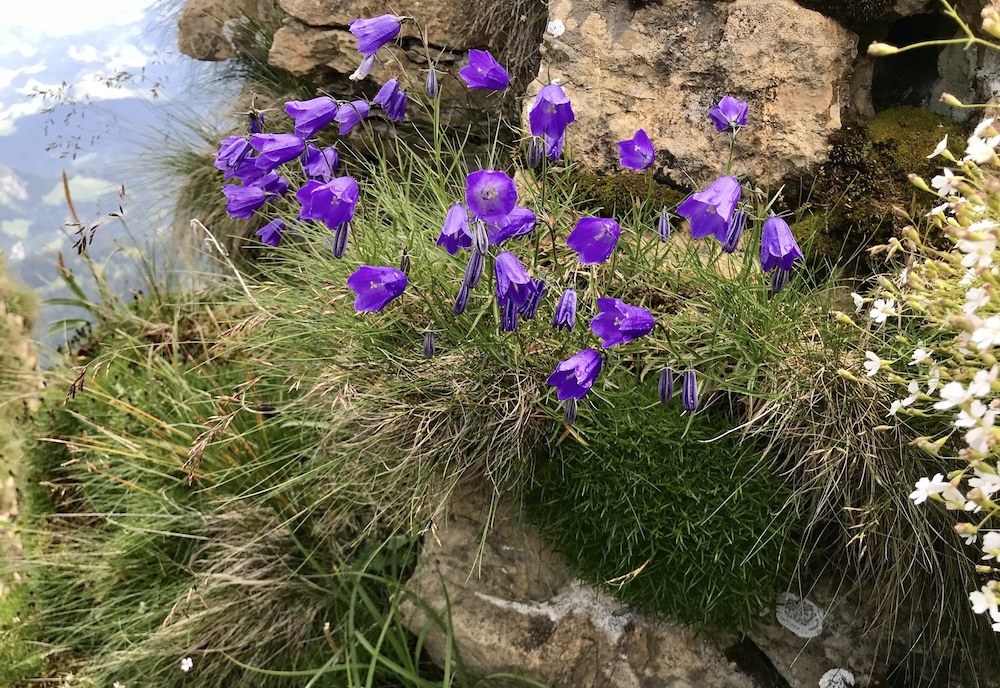
\includegraphics[width=1\linewidth]{images/campanula} \caption{*Campanula scheuchzeri* (Scheuchzer's Bellflower) in the Swiss Alps. Photo: M. Tobler}\label{fig:campanula}
\end{figure}

Studying evolutionary biology has helped me to address these questions. As a scientific discipline, evolutionary biology fundamentally seeks to understand biodiversity and its origins. Evolution is the unifying theory of biology because it provides a simple explanation for the patterns of similarities and differences we can observe among all living things, which ultimately forms the framework in which researchers across disciplines address questions about the living world. It does so by addressing both proximate and ultimate causes of organismal function. Proximate questions primarily focus on explaining organismal function in terms of intrinsic and environmental factors (these are sometimes referred to \emph{how} questions). For example, when we consider a peacocks magnificent tail feathers and coloration, how did environmental cues and changes in hormone levels initiate the development of these secondary sexual traits, and what genes might be involved in controlling there expression? In contrast, ultimate questions explain organismal function in terms of the evolutionary forces acting on them (sometimes referred to as why questions): why did the peacock evolve its exuberant traits, what are the traits' functions and how do they impact the fitness of its carrier?

Understanding how organisms work, how their traits allow them to survive in the peculiar environments they find themselves in, and how those traits came to be did not take out the wonder out of my fascination with nature; rather, it filled me with a new level of appreciation for the intricacies of life. I think that is \emph{the grandeur} Darwin was alluding to at the end of \emph{The Origin of Species}. Or, as another famous evolutionary biologist put it:

\begin{quote}
``Nothing in biology makes sense except in the light of evolution. {[}\ldots{]} Seen in the light of evolution, biology is, perhaps, intellectually the most satisfying and inspiring science. Without that light it becomes a pile of sundry facts, some of them interesting or curious, but making no meaningful picture as a whole.''

― Dobzhansky, 1973
\end{quote}

\hypertarget{beyond-understanding-biodiversity}{%
\section*{Beyond Understanding Biodiversity}\label{beyond-understanding-biodiversity}}
\addcontentsline{toc}{section}{Beyond Understanding Biodiversity}

Simply put, evolution is the change in heritable traits of populations that occurs across successive generations. Today, we have a nuanced understanding of the mechanisms that contribute to the evolutionary process. We are disentangling the genomic basis of traits relevant for organismal function, we are identifying the evolutionary forces---like natural selection---that determine what traits are passed on from one generation to the next, and we try to link these mechanisms to observable evolutionary outcomes, like adaptation, cooperation, and speciation. Applying these approaches has allowed us to explore many aspects of biodiversity, including the reasons behind sexual dimorphism, puzzling social behaviors, variation in life history traits, and even our own human origins.

The scientific reach of evolutionary biology, however, has long since eclipsed a basic understanding of the origins and function of biodiversity; the power of evolutionary analyses is now applied to address some of the major scientific challenges we face as a society: How will nature respond to the rapid environmental changes caused by human activities? How do we safeguard food production for a rapidly growing population? Why are there cancers and other diseases, and what can their origins tell us about prevention and treatment? How do we limit the spread of antibiotic-resistant pathogens? And how can we predict and limit the spread of emerging infectious diseases?

During this semester, we will cover both basic and applied aspects of evolution. So whether you are a bit of a naturalist---like myself---who tries to better understand the world, or whether you aspire to address some of the major environmental and public health issues we face as a society, I hope you will find something to take away from this class.

\hypertarget{an-overview-of-the-semester}{%
\section*{An Overview of the Semester}\label{an-overview-of-the-semester}}
\addcontentsline{toc}{section}{An Overview of the Semester}

The semester, and accordingly this book, is structured into four parts, each with multiple chapters that build on each other. Each chapter corresponds to a weekly module.

\hypertarget{part-1-the-basics}{%
\subsection*{Part 1: The Basics}\label{part-1-the-basics}}
\addcontentsline{toc}{subsection}{Part 1: The Basics}

In the first part of our journey, we will establish the basics of evolutionary biology. \href{what-evolution-is.html}{\textbf{Chapter 1}} introduces the concept of evolution and provides some historical context of how Darwin conceived his idea of ``descent with modification'' to describe the pattern of evolution. Treating the idea of evolution as a hypothesis, we will also develop testable predictions that can be verified through observation or experimentation. \href{evidence-for-evolution.html}{\textbf{Chapter 2}} will take a closer look at those predictions, and we will explore different lines of evidence that evolution has been---and still is---happening. Finally, \href{natural-selection-a-mechanism-for-change.html}{\textbf{Chapter 3}} will introduce Darwin's other big idea, natural selection, which describes a mechanism that can account for the tendency of organisms having traits well suited to the environments they live in.

\hypertarget{part-2-a-genetic-perspective-on-evolution}{%
\subsection*{Part 2: A Genetic Perspective on Evolution}\label{part-2-a-genetic-perspective-on-evolution}}
\addcontentsline{toc}{subsection}{Part 2: A Genetic Perspective on Evolution}

The second part takes a 21\textsuperscript{st} century perspective on evolution and closes a critical gap in Darwin's original ideas---namely, the mechanisms underlying heredity. We will integrate your knowledge of modern genetics with evolutionary principles to analyze changes in the genetic composition of populations through time. \href{the-raw-materials-for-evolution.html}{\textbf{Chapter 4}} will explore how different types of mutations impact the expression of phenotypic traits and provide the raw material for evolutionary change. In addition, we will learn how evolutionary biologists quantify genetic variation in populations and use that data to infer whether or not evolutionary forces are acting on a population. In \href{evolutionary-mechanisms-i-modeling-natural-selection.html}{\textbf{Chapter 5}} and \href{evolutionary-mechanisms-ii-mutation-genetic-drift-and-migration.html}{\textbf{Chapter 6}}, we will integrate evolution and genetics and use mathematical models to explore how natural selection interacts with other evolutionary forces (mutation, genetic drift, and migration) to shape the genetic composition of populations. In \href{molecular-evolution.html}{\textbf{Chapter 7}}, we will investigate the evolution of DNA sequences, explore the molecular signatures of selection, and see what we can uncover about historical processes simply by interpreting patterns of DNA sequence variation. And finally, in \href{the-evolution-of-quantitative-traits.html}{\textbf{Chapter 8}}, will learn about basic quantitative genetic approaches used to study the evolution of complex phenotypic traits controlled by many genes at once.

\hypertarget{part-3-evolutionary-outcomes-in-the-real-world}{%
\subsection*{Part 3: Evolutionary Outcomes in the Real World}\label{part-3-evolutionary-outcomes-in-the-real-world}}
\addcontentsline{toc}{subsection}{Part 3: Evolutionary Outcomes in the Real World}

The third part of the book explores the outcomes of natural selection and other evolutionary forces. \href{adaptation-and-phenotypic-plasticity.html}{\textbf{Chapter 9}} focuses on how we can infer adaptation in natural populations. We will explore the concept of phenotypic plasticity, why it can complicate the inference of adaptation, and how plasticity itself can be the outcome of adaptive evolution. In \href{intraspecific-interactions-social-behavior-and-sexual-selection.html}{\textbf{Chapter 10}}, we will focus on how evolution has shaped the social interactions between individuals of the same species, learning about kin and sexual selection. Finally, \href{speciation-1.html}{\textbf{Chapter 11}} investigates how new species arise. We will discuss speciation as a gradual process that is shaped by the same evolutionary forces that influence the evolution of phenotypic traits within species.

\hypertarget{part-4-applied-evolutionary-biology}{%
\subsection*{Part 4: Applied Evolutionary Biology}\label{part-4-applied-evolutionary-biology}}
\addcontentsline{toc}{subsection}{Part 4: Applied Evolutionary Biology}

The last part of the book focuses on the application of evolutionary theory in the context of human nature and human health. \href{evolutionary-medicine-i-aging-and-diseases-of-civilization.html}{\textbf{Chapters 12}} and \href{evolutionary-medicine-ii-evolving-pathogens.html}{\textbf{Chapter 13}} explore how evolutionary principles are applied in modern medicine. We will discuss why we age and how modern lifestyles are connected to the development of a wide variety of health conditions commonly named ``diseases of civilization''. In addition, we will explore how a better understanding of pathogen evolution allows for the development of concrete management strategies that can impact the spread of diseases. Finally, \href{human-origins-and-human-mediated-evolution.html}{\textbf{Chapter 14}} includes an overview of human origins and discusses how the sequencing of ancient DNA has shed new light into our own history.

\hypertarget{how-to-use-this-book}{%
\section*{How to Use This Book}\label{how-to-use-this-book}}
\addcontentsline{toc}{section}{How to Use This Book}

This book is not designed to provide a comprehensive overview of current evolutionary biology. Rather, it is supposed to provide a succinct introduction to evolutionary thought revolving around theory, evidence, and practice:

\begin{itemize}
\tightlist
\item
  I will introduce some of the \textbf{theoretical cornerstones and core concepts} of modern evolutionary biology. The goal is for you to be able to apply these concepts and articulate testable hypotheses that explain natural phenomena from an evolutionary perspective.
\item
  You will become familiar with the diversity of \textbf{empirical approaches and lines of evidence} that scientists use to address evolutionary hypotheses.
\item
  You will practice approaching problems like scientists and evaluate data to address evolutionary hypotheses. To do so, you will learn how to program in R to \textbf{analyze and visualize data} and articulate your interpretations and conclusions.
\end{itemize}

In accordance with these goals, each chapter will provide you with a conceptual introduction to the topic. There is not much emphasis on examples, as we will explore those together in our class meetings. Each chapter also includes additional resources that you can explore if you have difficulties understanding or if you want to explore a topic in more detail. To help you with the R exercises, each chapter also provides you with additional background on case studies and R programming tutorials that help you to develop the necessary skills. Finally, each chapter ends with a series of reflection questions that will prompt you to review your learning. For quick reference, Appendix A summarizes some of the key R code you will work with in the class, and Appendix B offers all exercises for quick download.

Please note that this resource has been developed and optimized to be used as an HTML book that can be accessed with any web browser. Accessing the book this way allows you to make full use of the dynamical content and R components, which are more limited if you print. Plus, you can save a bunch of trees:)

\hypertarget{references}{%
\section*{References}\label{references}}
\addcontentsline{toc}{section}{References}

\begin{itemize}
\tightlist
\item
  Darwin, C (1859): \emph{On the origin of species based on natural selection, or the preservation of favoured races in the struggle of life.} London: John Murray.
\item
  Dobzhansky, T (1973): Nothing in biology makes sense except in the light of evolution. \emph{The American Biology Teacher} 35: 125--129.
\end{itemize}

\hypertarget{front-matters}{%
\chapter*{Front Matters}\label{front-matters}}
\addcontentsline{toc}{chapter}{Front Matters}

\hypertarget{acknowledgments}{%
\section*{Acknowledgments}\label{acknowledgments}}
\addcontentsline{toc}{section}{Acknowledgments}

I alternate teaching K-State's Evolution course (BIOL 520) with Tom Platt, and over the years, John Coffin, Ryan Greenway, Madison Nobrega, and Libby Wilson have served as graduate teaching assistants. They have all made immeasurable contributions to the development of the learning materials included here. I especially thank Madison Nobrega for her relentless editing; her input has greatly improved this text. Emily G. Finch from the Center for the Advancement of Digital Scholarship at the Kansas State University Libraries and Greg Dressman, Director of Enterprise Server Technologies at Kansas State University\textbf{,} provided critical logistical support.

This book was made possible with the support of a grant from the \href{https://www.lib.k-state.edu/open-textbook}{The Open/Alternative Textbook Initiative at Kansas State University}.

Last but not least, many thanks to the past students in BIOL 520 at K-State. It was your input that lead to this resource and that helps me to continuously improve it. Especially, the following people have graciously provided feedback on writing and content: Shaun Baughman, Caroline Gatschet, Aaron George, Kate Odgers, and Andy Su.

\hypertarget{copyright}{%
\section*{Copyright}\label{copyright}}
\addcontentsline{toc}{section}{Copyright}

© 2022 by Michi Tobler


\includegraphics[width=1.22in]{images/cc}

This work is licensed under a \href{https://creativecommons.org/licenses/by-nc-sa/4.0/}{Creative Commons Attribution-NonCommercial-ShareAlike 4.0 International License}. You are free to copy and redistribute the material in any medium or format, and to remix, transform, and build upon the material provided you give the original author credit (attribution), you are not using the material for commercial purposes (NonCommerical), and you distribute your work under the same license as the original (ShareAlike).

If you would like to adopt and use this resource in any way, feel free to contact \href{mailto:tobler@ksu.edu}{Michi Tobler} to obtain a copy of all source files.

\hypertarget{about-the-author}{%
\section*{About the Author}\label{about-the-author}}
\addcontentsline{toc}{section}{About the Author}

Michi Tobler is a Professor in the \href{https://www.k-state.edu/biology/}{Division of Biology} at Kansas State University in Manhattan, KS. His research focuses on mechanisms of adaptation and speciation, primarily using extremophile fishes as study systems. You can learn more about our research on his lab website: \url{https://sulfide-life.info/}

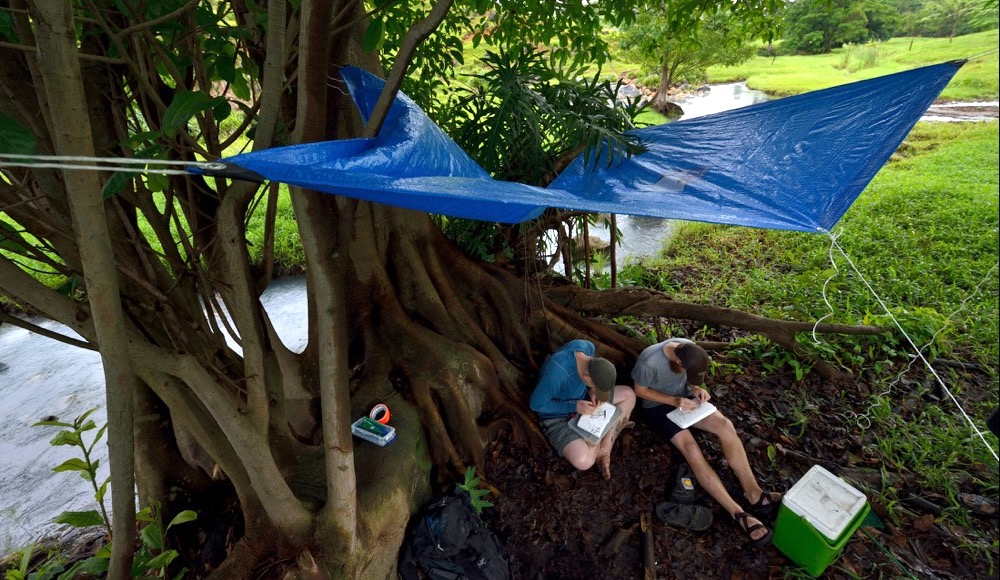
\includegraphics[width=1\linewidth]{images/fieldlab}

\hypertarget{part-basic-concepts}{%
\part{Basic Concepts}\label{part-basic-concepts}}

\hypertarget{what-evolution-is}{%
\chapter{What Evolution Is}\label{what-evolution-is}}

The notion of an ever-changing world is a relatively new idea in Western cultures. Dating back to the teachings of Greek philosophers, the world was long seen as permanent and unchanging. Its inhabitants were thought to be arranged on scale from lower to higher beings by a divine creator, with humans at the very top of the hierarchy. Until the early 1800s, most naturalists were primarily concerned with describing and cataloging life, which led to the modern classification system originally developed by the Swedish biologist Carolus Linnaeus.

By the time Charles Darwin was born in the early 19\textsuperscript{th} century, evidence for a changing world was accumulating. Geologists started to contemplate how slow, gradual processes could carve canyons into stone and change the course of rivers. The discovery of fossils indicated the past existence of organisms vastly different than today's and suggested a rich history with continuous change. And some scholars, like the French biologist Jean-Baptiste Lamarck (Figure \ref{fig:lamarck}), started to formulate theories that could potentially explain the diversity of life. Budding evolutionary thought was not limited to Western cultures, and there were a number of pre-Darwinian Muslim scholars who articulated evolutionary ideas as well (Malik et al.~2018).

\begin{figure}
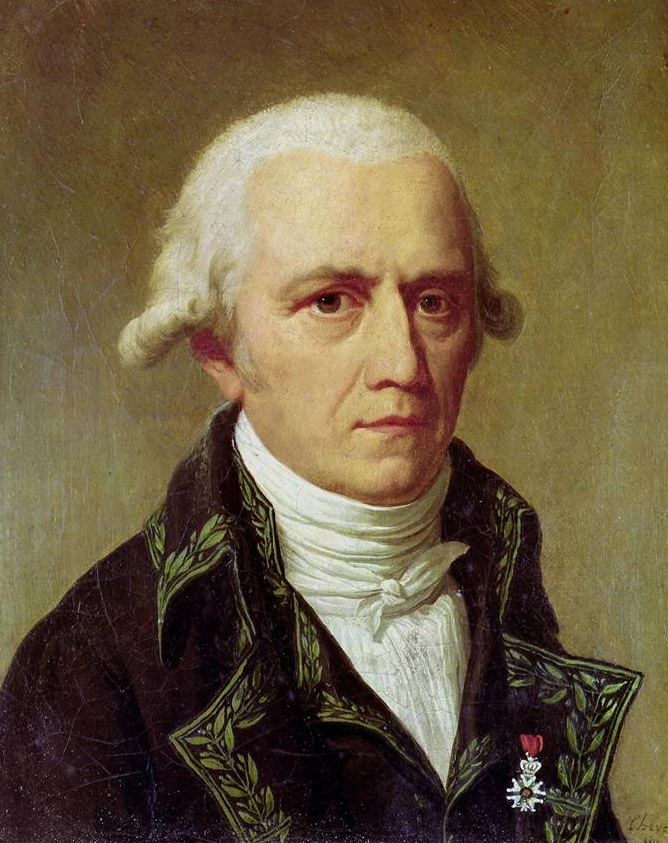
\includegraphics[width=0.5\linewidth]{images/Jean-Baptiste_de_Lamarck} \caption{Jean-Baptiste de Monet Chevalier de Lamarck. Painted by Charles Thévenin, [Public Domain](https://creativecommons.org/share-your-work/public-domain/).}\label{fig:lamarck}
\end{figure}

It was Lamarck, inspired by the similarities he observed across different species, who formulated the first theory of evolution. Lamarck argued that life was inevitably driven towards increasing complexity, essentially progressing along the scale from lower to higher beings established by the Greeks. He envisioned that simpler life forms, like microbes, continuously arise and eventually develop into higher forms, like plants and animals. Lamarck also believed that progress along this hierarchy allowed organisms to adapt to their environment, which was driven by an ``inner need''. He thought that the continuous use of a particular organ allowed for its proliferation and subsequent inheritance to the next generation. Perhaps most famously, Lamarck explained that the long neck of the giraffe was the product of a continuous stretching toward leaves high on the trees. So, across many generations of stretching, giraffe necks gradually reached their current size.

\hypertarget{darwin-and-the-conception-of-a-new-idea}{%
\section{Darwin and the Conception of a New Idea}\label{darwin-and-the-conception-of-a-new-idea}}

When Darwin boarded the British Navy Ship HMS Beagle as a 22-year old, he was already well trained in geology, chemistry, and natural history. Darwin was hired as an unofficial naturalist and companion to the captain of the ship, Robert FitzRoy, and the five-year journey around the world allowed young Darwin to collect evidence of a changing world (Figure \ref{fig:beaglemap}).

\begin{figure}
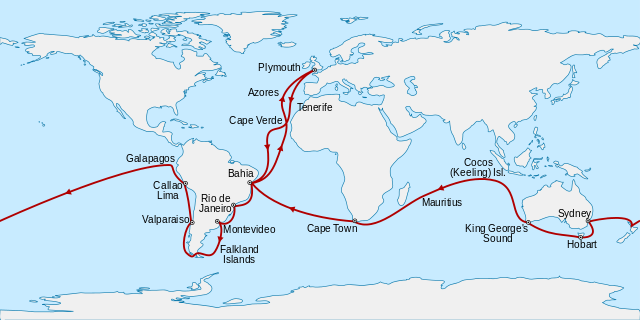
\includegraphics[width=1\linewidth]{images/voyage_beagle-01} \caption{Map of the Voyage of the Beagle. Map: Sémhur, [CC BY-SA 4.0](https://creativecommons.org/licenses/by-sa/4.0/).}\label{fig:beaglemap}
\end{figure}

Darwin's visit to the Galapagos Islands, and the specimens of reptiles and birds that he collected there, proved to be particularly inspiring. The Galapagos are an archipelago of 21 small islands, located over 900 kilometers off the coast of Ecuador, and situated right on the equator. Darwin not only noticed that the fauna of these islands was dominated by animals found nowhere else, but there also were differences in the species from one island to the next. Most importantly, bird specimens that Darwin believed to be blackbirds, warblers, wrens, and finches due to their different beak morphologies later all turned out to be just finches---the Darwin's finches we know today (Figure \ref{fig:finches}). In his own words:

\begin{quote}
``I have stated, that in the thirteen species of ground-finches, a nearly perfect gradation may be traced, from a beak extraordinarily thick, to one so fine, that it may be compared to that of a warbler. {[}\ldots{]} Seeing this gradation and diversity of structure in one small, intimately related group of birds, one might really fancy that from an original paucity of birds in this archipelago, one species had been taken and modified for different ends.''

--- Darwin, 1889
\end{quote}

If all the species were created with traits that fit the environments in which they are now found, why would the finches of the Galapagos Islands be so different from one another? Why do closely related species occupy niches that are filled by very different taxa in other regions? Observations like these, which Darwin made at many destinations throughout his travels, led him to suspect that the species we observe today have evolved from a shared ancestor.

\begin{figure}
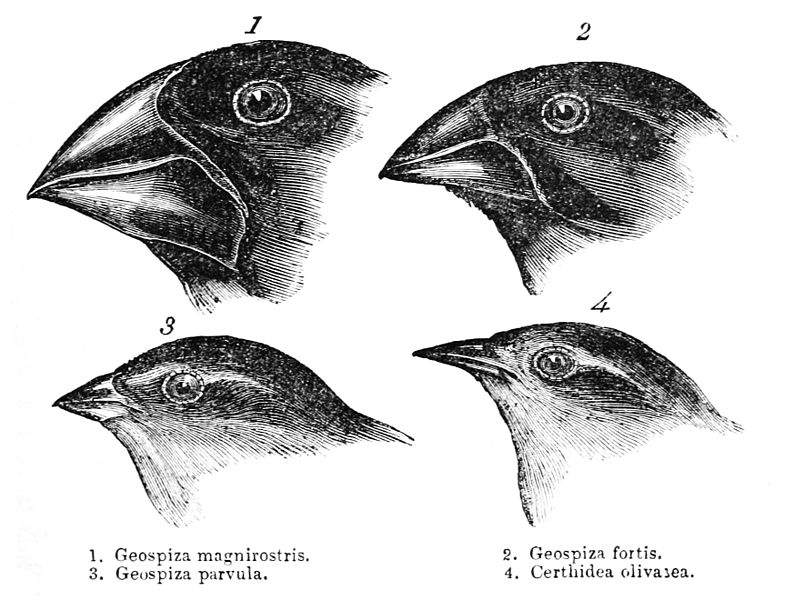
\includegraphics[width=1\linewidth]{images/Darwin_finches} \caption{Examples of Darwin's finches or Galapagos finches. Note the stark variation in beak sizes among the four species. Drawn by John Gould, [Public Domain](https://creativecommons.org/share-your-work/public-domain/).}\label{fig:finches}
\end{figure}

Upon his return to England in 1836, Darwin settled near London and never traveled abroad again. Nonetheless, he remained a prolific scholar writing monographs about various topics, from geology to barnacles. Darwin was also a passionate pigeon breeder, and it was this unlikely hobby that provided additional insights for the formulation of his ideas. It led him to think about the forces that could drive the modification of species from one common ancestor to different descendants:

\begin{quote}
``It is, therefore, of the highest importance to gain a clear insight into the means of modification. {[}\ldots{]} At the commencement of my observations it seemed to me probable that a careful study of domesticated animals and of cultivated plants would offer the best chance of making out this obscure problem.''

--- Darwin, 1859
\end{quote}

In his endeavors of pigeon breeding, Darwin noticed two critical things: (1) Offspring tended to inherit the traits of their parents. (2) If he carefully selected breeders with desired traits generation after generation, he was able to shape the variation of colors, morphologies, and behaviors in his flock. It was his meticulous work as a natural historian, collecting evidence for his emerging ideas for over two decades, that ultimately allowed Darwin to formulate the basic tenets of evolutionary biology that still hold up today, after more than 150 years of scrutiny by the scientific community.

\hypertarget{two-fundamental-insights}{%
\section{Two Fundamental Insights}\label{two-fundamental-insights}}

\hypertarget{predictions}{%
\subsection{The Pattern: Evolution is Descent with Modification}\label{predictions}}

The first of Darwin's fundamental insights was the formal description of evolution as we understand it today. He described evolution as \emph{descent with modification}, postulating the common ancestry of all living things. Hence, different species did not arise independently, but they derived from preexisting form. This insight arose from a careful analysis of patterns of similarities across species. Species that share a recent common ancestor share traits precisely because they inherited them the shared ancestor. More distantly related taxa exhibit differences in their traits, because they have been on independent evolutionary trajectories for longer periods of time. This perspective describes the observable \emph{pattern of evolution}.

Given Darwin's insight, here is a simple definition of evolution that we will rely on for now. As you will see, there are multiple modern definitions of evolution, and we will revisit different definitions throughout the book.

Definition: Evolution

Evolution is the change in the inherited traits of a population across successive generations, ultimately leading to the transformation of species through time (both in terms of changes of traits that occur within species and the origin of new species).

The power of Darwin's idea of descent with modification is that we can treat it as a scientific hypothesis with empirically testable predictions. If Darwin's notion of evolution was right, we should be able to uncover evidence that:

\begin{enumerate}
\def\labelenumi{\arabic{enumi}.}
\tightlist
\item
  Species change through time (microevolution).
\item
  Lineages split to form new species (speciation).
\item
  Novel forms derive from earlier forms (macroevolution).
\item
  Species are not independent but connected by descent from a common ancestor (common ancestry and homology).
\item
  Earth and life on Earth are old (deep time).
\end{enumerate}

We will revisit these predictions and examine the evidence for evolution in detail in \href{evidence-for-evolution.html}{Chapter 2}.

\hypertarget{the-process-natural-selection-is-a-mechanism-of-evolution}{%
\subsection{The Process: Natural Selection is a Mechanism of Evolution}\label{the-process-natural-selection-is-a-mechanism-of-evolution}}

The second of Darwin's fundamental insights was the inception of a mechanism that could produce the observable pattern we call evolution (i.e., change in inherited traits across generations), which Darwin named natural selection.

Definition: Natural Selection

Natural selection is the process in which individuals with a particular trait exhibit higher reproductive success than individuals without that trait.

Natural selection explains how the traits of a population change through time, and why organisms are well suited for their environment. Individuals that exhibit traits that are advantageous under certain environmental conditions have a higher chance of surviving and reproducing, making a disproportional contribution to the offspring of the next generation. If the relevant traits are heritable, their frequency increases across subsequent generations. This process not only leads to change in populations across generations, but said change specifically pertains to traits that are important for survival and reproduction in a given environmental context. In other words, the action of natural selection directly leads to adaptation. We will take a close look at how natural selection works in \href{natural-selection-a-mechanism-for-change.html}{Chapter 3}.

\hypertarget{distinguishing-between-pattern-and-process}{%
\subsection{Distinguishing between Pattern and Process}\label{distinguishing-between-pattern-and-process}}

A key misconception is that evolution and natural selection are the same. People often use the two terms interchangeably, conflating patterns and processes of evolution. Distinguishing between the two is critical, because evolution and natural selection do not have to go in unison.

Evolution is a historical pattern of change that can---but does not have to---be caused by natural selection. Evolutionary change can also be driven by other forces that impact the composition of populations across generations. In Part II of this book, we will examine evolutionary forces other than natural selection, which include mutation, genetic drift, and migration. In natural populations, these four forces interact to shape evolutionary change across time.

It is also important to note that the action of natural selection does not necessarily lead to evolution. Natural selection can only cause evolution when it acts on heritable traits that are transmitted from parent to offspring. If that is the case, the offspring of successful individuals will carry the same traits that made their parents successful. However, not all traits are heritable. For example, selection on individuals exhibiting high muscle mass does not translate to evolutionary change if that muscle mass was acquired through exercise and diet. If natural selection acts on non-heritable traits, there is no evolutionary change.

Explore More: Misconceptions about Evolution

Despite the broad scientific consensus on the importance of evolutionary theory in understanding the diversity of life, people hold many misconceptions about evolutionary theory and processes, its implications, and its relation to religious beliefs. I encourage you to explore the fantastic \href{https://evolution.berkeley.edu/evolibrary/misconceptions_faq.php}{resource provided by The University of California Museum of Paleontology, which lists common misconceptions about evolution and clarifies these misconceptions}.

\hypertarget{population-thinking}{%
\subsection{Population Thinking}\label{population-thinking}}

Darwin's fundamental insights were possible because of a fundamental shift in how he thought about biological entities, from a typological perspective to what Mayr (1982) called ``population thinking''. Prior to Darwin, scholars viewed individual organisms as imperfect representations of a central Platonic type (the perfect manifestation of a species). Variation among individuals was considered to be meaningless noise that was either ignored or seen as a nuisance when describing and classifying species. In contrast, population thinking rejects the notion of an ideal representative and instead focus on the variants found within populations. Variation among individuals is not just meaningless noise that represents different degrees of imperfections from a preconceived idea, but it is the raw material for evolutionary change. In other words, what was meaningless noise to naturalists prior to Darwin suddenly became the very focus of evolutionary studies after. Mayr (1982) argued that this paradigm shift was one of Darwin's most important contributions to modern biology.

\hypertarget{practical-skills-getting-started-with-r}{%
\section{Practical Skills: Getting Started with R}\label{practical-skills-getting-started-with-r}}

During this course, you will learn about evolution \emph{and} practice being a scientist by visualizing and interpreting data on a weekly basis. To do so, we will use an open-source software called R. This section provides instructions for installing R and a companion program (RStudio) on your Mac or PC.

\hypertarget{what-are-r-and-rstudio}{%
\subsection{What are R and RStudio?}\label{what-are-r-and-rstudio}}

R is a programming language for statistical analysis and data visualization, and over the past decades, it has become one of the most critical and universally used tools in the life sciences. RStudio is a convenient interface that allows you to easily write, organize, and execute your R code; it's the program we will use throughout the semester for weekly assignments. Note that RStudio will not run unless R is already installed.

\hypertarget{installing-r}{%
\subsection{Installing R}\label{installing-r}}

To run R and RStudio on your system, complete the following steps in the right order (\emph{i.e.}, you need to install R before you can install RStudio). Although we recommend the use of Windows or Mac OS for this class, R is also available for \href{https://cran.r-project.org/bin/linux/ubuntu/}{Linux}, and it can be installed on \href{https://blog.sellorm.com/2018/12/20/installing-r-and-rstudio-on-a-chromebook/}{Google Chromebooks}. Please note that any code used in this course has not been troubleshot on the latter two platforms.

\hypertarget{for-windows}{%
\subsubsection*{For Windows}\label{for-windows}}
\addcontentsline{toc}{subsubsection}{For Windows}

\begin{itemize}
\item
  \href{https://cran.r-project.org/bin/windows/base/}{Download the binary setup file for R 4.2.x}
\item
  Open the downloaded *.exe file and follow the instructions to install R
\item
  \href{https://cran.r-project.org/bin/windows/Rtools/}{Download the binary setup file for Rtools40}
\item
  Open the downloaded *.exe file and follow the instructions to install Rtools
\end{itemize}

\hypertarget{for-mac}{%
\subsubsection*{For Mac}\label{for-mac}}
\addcontentsline{toc}{subsubsection}{For Mac}

\begin{itemize}
\item
  Check the version on your operating system (click the Apple logo on your desktop and choose ``About This Mac''). If your macOS version is 10.14 or older, please \href{https://support.apple.com/en-us/HT201541}{first update your computer to a newer macOS version}. If you do not update your computer first, R and RStudio may still install properly, but you will run into compatibility issues later in the semester when use different packages within R.
\item
  Download the .pkg file for R 4.2.x form the following link: \url{https://cran.r-project.org/bin/macosx/}
\item
  Open the downloaded *.pkg file and follow the instructions to install R
\end{itemize}

\hypertarget{installing-rstudio}{%
\subsection{Installing RStudio}\label{installing-rstudio}}

\href{https://www.rstudio.com/products/rstudio/download/}{Download the free, open-source version of RStudio Desktop} by choosing the appropriate installer file for your operating system and then run it to install RStudio. If you are using Mac, make sure to move the RStudio app to your actual Applications folder (rather than starting it from the disk image).

\hypertarget{checking-the-successful-installation}{%
\subsection{Checking the Successful Installation}\label{checking-the-successful-installation}}

Once you completed the steps above, we recommend that you launch RStudio and make sure it starts without any errors. If the installation was successful, the RStudio interface should look something like Figure \ref{fig:interface}:

\begin{figure}
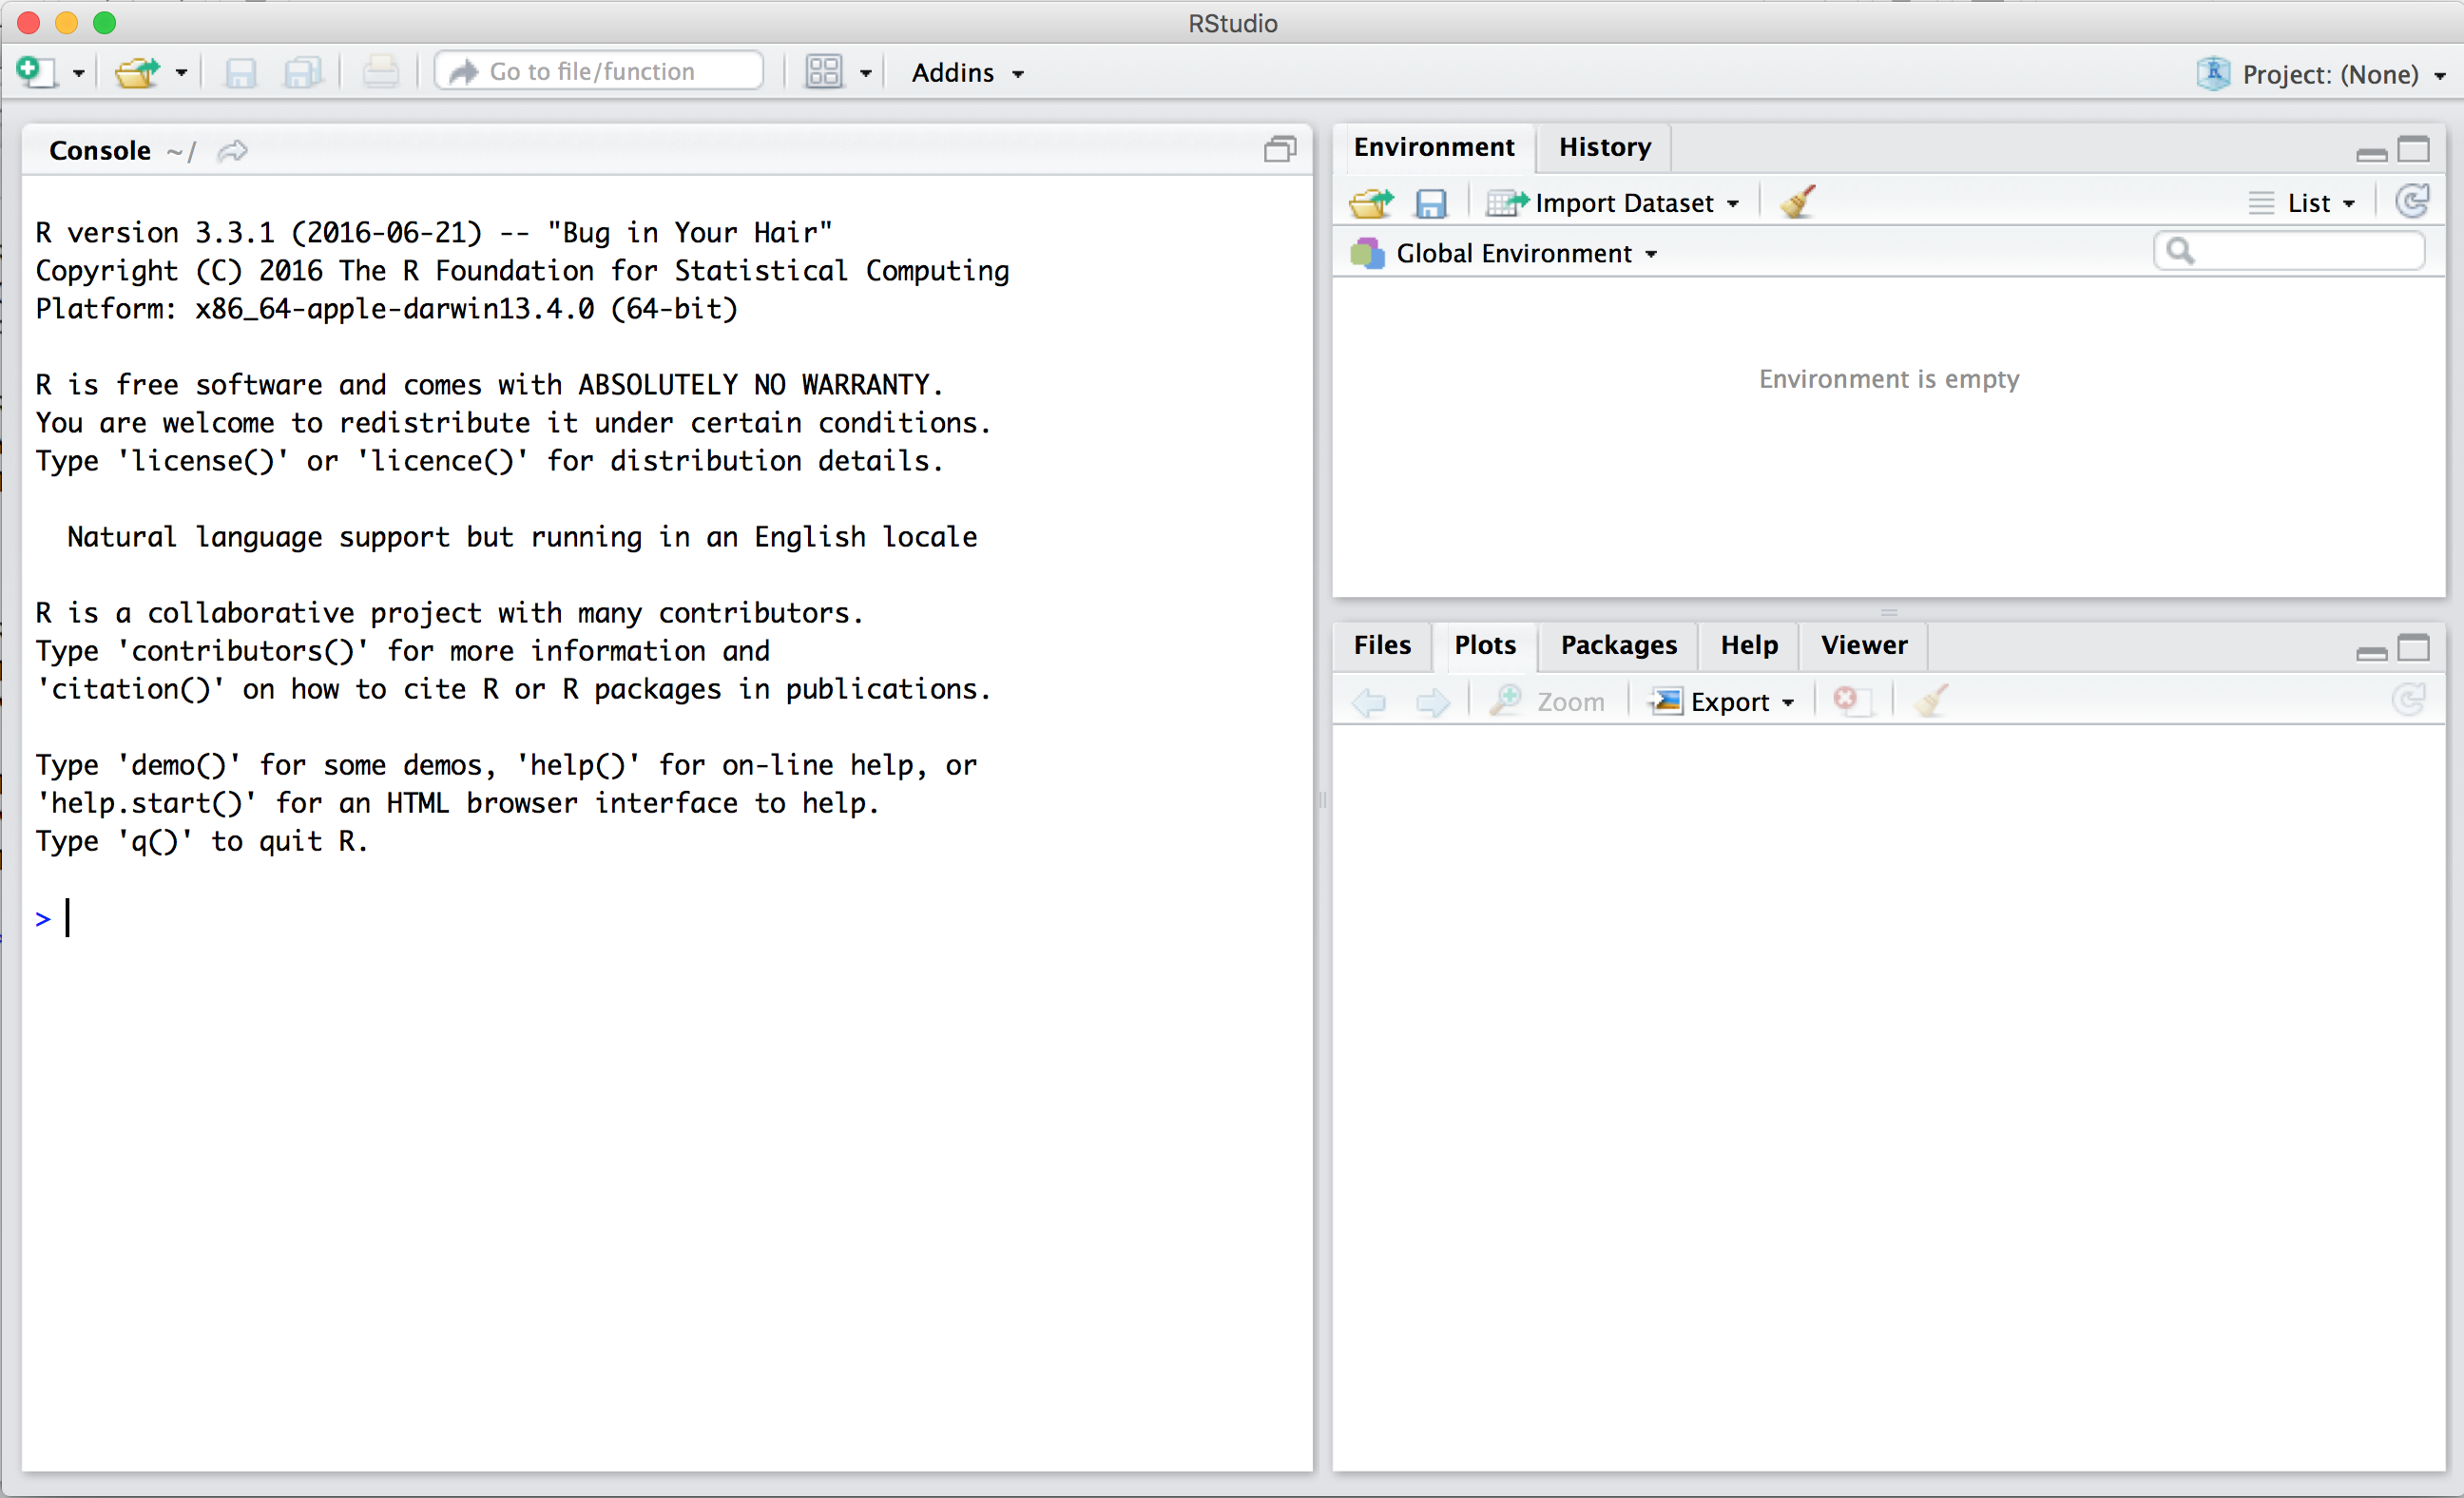
\includegraphics[width=1\linewidth]{images/rstudio_interface} \caption{Screenshot of the RStudio interface.}\label{fig:interface}
\end{figure}

\hypertarget{some-r-and-rstudio-basics}{%
\subsection{Some R and RStudio Basics}\label{some-r-and-rstudio-basics}}

This section was inspired by and used parts of ``\href{https://chem.libretexts.org/@go/page/7641}{Introduction to R}'' by \href{https://poldracklab.stanford.edu/}{Russell A. Poldrack}, published on \href{https://libretexts.org/}{LibreTexts} and licensed under \href{https://creativecommons.org/licenses/by-nc/4.0/}{CC BY-NC}.

Learning a programming language---like learning any language---can be intimidating. Still, it is a basic skill for any scientist. Starting in Chapter 2, you will work through R exercises that help you digest the basic concepts discussed in each chapter. We will show you exactly how to use RStudio to work through the exercises there. As you will see, most assignments in class will provide you with the majority of the code structure in a way that a few simple tweaks on your side will produce the desired outcome. But we encourage you to explore beyond what the exercises dictate. A willingness to experiment will make you a better programmer and scientist. Before we get to that stage, however, you need to build some basic fluency in R, so you can ease yourself into using this new tool.

\hypertarget{the-console-and-basic-r-prompts}{%
\subsubsection*{The Console and Basic R Prompts}\label{the-console-and-basic-r-prompts}}
\addcontentsline{toc}{subsubsection}{The Console and Basic R Prompts}

Let's begin with the fundamental building blocks of R and RStudio. As you open RStudio, the program window will look something like \protect\hyperlink{Fig1.4}{Figure 1.4}.The panel in the upper right contains your work space (Global Environment) as well as a history of the commands that you've previously entered. Any plots that you generate will show up in the panel in the lower right corner and you can also use that section to browse your folders for specific files. The panel on the left is where the action happens. It's called the Console. Every time you launch RStudio, it will have the same text at the top of the console telling you the version of R that you're running. Below that information is the command prompt (symbolized by \texttt{\textgreater{}}), where you can enter commands and R responds to those commands.

It's really simple, and you can try it out right now! Just type \texttt{2+2}, press enter, and R should respond right back with the response. It should look like this:

\begin{Shaded}
\begin{Highlighting}[]
\DecValTok{2}\SpecialCharTok{+}\DecValTok{2}
\end{Highlighting}
\end{Shaded}

\begin{verbatim}
## [1] 4
\end{verbatim}

R pretty much operates like a calculator and can perform any calculation you might need. R can also deal with logical variables, and respond to queries about whether logic statements are true or false. For example, you can use logical operators {[}\texttt{\textgreater{}} (greater than), \texttt{\textless{}} (smaller than), \texttt{==} (equals), \texttt{!=} (not-equals){]} to contrast statements, and R will assess them:

\begin{Shaded}
\begin{Highlighting}[]
\DecValTok{5}\SpecialCharTok{*}\DecValTok{2}\SpecialCharTok{\textgreater{}}\FunctionTok{sqrt}\NormalTok{(}\DecValTok{100}\NormalTok{) }\CommentTok{\#note that sqrt starts for square{-}root}
\end{Highlighting}
\end{Shaded}

\begin{verbatim}
## [1] FALSE
\end{verbatim}

\begin{Shaded}
\begin{Highlighting}[]
\DecValTok{5}\SpecialCharTok{*}\DecValTok{2}\SpecialCharTok{==}\FunctionTok{sqrt}\NormalTok{(}\DecValTok{100}\NormalTok{)}
\end{Highlighting}
\end{Shaded}

\begin{verbatim}
## [1] TRUE
\end{verbatim}

\hypertarget{working-with-variables}{%
\subsubsection*{Working with Variables}\label{working-with-variables}}
\addcontentsline{toc}{subsubsection}{Working with Variables}

One of the strengths of R is that it cannot only perform basic calculations using numbers, but it can handle variables, which are symbols that stand for values. You can designate a variable using \texttt{\textless{}-}. For example, we can assign the value 5 to x:

\begin{Shaded}
\begin{Highlighting}[]
\NormalTok{x }\OtherTok{\textless{}{-}} \DecValTok{5}
\end{Highlighting}
\end{Shaded}

Notice when you run that code, you created a new variable x with the value 5 that shows up in your work space on the top-right panel. Once you have a variable defined, you can use it in calculations and logic statements as described above:

\begin{Shaded}
\begin{Highlighting}[]
\NormalTok{x}\SpecialCharTok{\^{}}\DecValTok{2}
\end{Highlighting}
\end{Shaded}

\begin{verbatim}
## [1] 25
\end{verbatim}

\begin{Shaded}
\begin{Highlighting}[]
\NormalTok{x}\SpecialCharTok{==}\DecValTok{5}
\end{Highlighting}
\end{Shaded}

\begin{verbatim}
## [1] TRUE
\end{verbatim}

Designating variables allows you to write some complex code that processes data, and if you want to do the same thing with different data, you don't have to rewrite the code, you just redefine the input variables. For example you can designate three different variables:

\begin{Shaded}
\begin{Highlighting}[]
\NormalTok{x1 }\OtherTok{=} \DecValTok{16}
\NormalTok{x2 }\OtherTok{=} \DecValTok{12}
\NormalTok{x3 }\OtherTok{=} \DecValTok{2}
\end{Highlighting}
\end{Shaded}

If you use these variables in a complex equation, you need to just write the equation once, and you can tweak the input variables to explore the effects of different values.

\begin{Shaded}
\begin{Highlighting}[]
\NormalTok{x1}\SpecialCharTok{*}\NormalTok{(x1}\SpecialCharTok{+}\NormalTok{x2}\SpecialCharTok{+}\NormalTok{x3)}\SpecialCharTok{/}\NormalTok{(x1}\SpecialCharTok{\^{}}\DecValTok{2}\SpecialCharTok{+}\NormalTok{x2}\SpecialCharTok{\^{}}\DecValTok{2}\SpecialCharTok{+}\NormalTok{x3}\SpecialCharTok{\^{}}\DecValTok{2}\NormalTok{)}
\end{Highlighting}
\end{Shaded}

\begin{verbatim}
## [1] 1.188119
\end{verbatim}

\hypertarget{vectors}{%
\subsubsection*{Vectors}\label{vectors}}
\addcontentsline{toc}{subsubsection}{Vectors}

Variables are not only able to designate numbers, they can also designate lists of numbers (called vectors). You can create a vector (\texttt{y} in this case) using the \texttt{c()} function, and you can then call on \texttt{y} using \texttt{print()} for R to display the vector in the console:

\begin{Shaded}
\begin{Highlighting}[]
\NormalTok{y }\OtherTok{\textless{}{-}} \FunctionTok{c}\NormalTok{(}\DecValTok{1}\NormalTok{,}\DecValTok{12}\NormalTok{,}\DecValTok{2}\NormalTok{,}\DecValTok{14}\NormalTok{)}
\FunctionTok{print}\NormalTok{(y)}
\end{Highlighting}
\end{Shaded}

\begin{verbatim}
## [1]  1 12  2 14
\end{verbatim}

If you execute this code, you will again see the creation of a new variable y in your work space, which corresponds to a vector with four numbers.

You can call numbers within a particular vector by using square brackets along with the variable name and a the number that refers to a location within the vectors. So, if we want to extract the 3\textsuperscript{rd} number in our vector \texttt{y}, we simply type:

\begin{Shaded}
\begin{Highlighting}[]
\NormalTok{y[}\DecValTok{3}\NormalTok{]}
\end{Highlighting}
\end{Shaded}

\begin{verbatim}
## [1] 2
\end{verbatim}

We can also extract a range of values by using a colon. Let's say you want to extract the last two numbers in our vector:

\begin{Shaded}
\begin{Highlighting}[]
\NormalTok{y[}\DecValTok{3}\SpecialCharTok{:}\DecValTok{4}\NormalTok{]}
\end{Highlighting}
\end{Shaded}

\begin{verbatim}
## [1]  2 14
\end{verbatim}

Finally, you can modify specific values within a vector by just combining some of the code you have already learned so far. For example, you can change the second value in our vector \texttt{y} from a 12 to 4:

\begin{Shaded}
\begin{Highlighting}[]
\NormalTok{y[}\DecValTok{2}\NormalTok{] }\OtherTok{\textless{}{-}} \DecValTok{4}
\NormalTok{y}
\end{Highlighting}
\end{Shaded}

\begin{verbatim}
## [1]  1  4  2 14
\end{verbatim}

\hypertarget{using-functions}{%
\subsubsection*{Using Functions}\label{using-functions}}
\addcontentsline{toc}{subsubsection}{Using Functions}

R can execute a wide variety of functions that take some input and provide an output based on the input. Functions can be applied to a simple number. For example the \texttt{sqrt()} function calculates the square-root of an input number. We can use it on our variable x that we defined above:

\begin{Shaded}
\begin{Highlighting}[]
\FunctionTok{sqrt}\NormalTok{(x)}
\end{Highlighting}
\end{Shaded}

\begin{verbatim}
## [1] 2.236068
\end{verbatim}

We can also apply the same function to a vector, in which case the function is applied to every number in the vector:

\begin{Shaded}
\begin{Highlighting}[]
\FunctionTok{sqrt}\NormalTok{(y)}
\end{Highlighting}
\end{Shaded}

\begin{verbatim}
## [1] 1.000000 2.000000 1.414214 3.741657
\end{verbatim}

Sometimes we want to use the output of one function as an input for another function. In this case, it makes sense to store the output of a function in a new object:

\begin{Shaded}
\begin{Highlighting}[]
\NormalTok{sqrt.y }\OtherTok{\textless{}{-}} \FunctionTok{sqrt}\NormalTok{(y)}
\FunctionTok{print}\NormalTok{(sqrt.y)}
\end{Highlighting}
\end{Shaded}

\begin{verbatim}
## [1] 1.000000 2.000000 1.414214 3.741657
\end{verbatim}

Note that this code again created a new object called \texttt{sqrt.y} in your work space, and you can call on it using \texttt{print()} to display it in the console. We can now also use the new values as input for another function. For example, we can calculate the average of these values using the \texttt{mean()} function:

\begin{Shaded}
\begin{Highlighting}[]
\FunctionTok{mean}\NormalTok{(sqrt.y)}
\end{Highlighting}
\end{Shaded}

\begin{verbatim}
## [1] 2.038968
\end{verbatim}

Over the course of the semester, you will get to know a wide variety of functions in R that will allow you to make complex plots and analyze genetic and phenotypic data to make evolutionary inferences. R already knows a large number of functions upon installation, but you can essentially teach it limitless new functions by installing so-called libraries (or packages). There are \href{https://cran.r-project.org/web/packages/available_packages_by_name.html}{thousands of libraries for R}, and they contain functions to analyze and visualize all kinds of biological data, from the structure of genomes to the composition of ecological communities. You will learn how to install new libraries and apply the functions they contain in \href{evidence-for-evolution.html\#libraries}{Chapter 2}.

\hypertarget{data-frames}{%
\subsubsection*{Data Frames}\label{data-frames}}
\addcontentsline{toc}{subsubsection}{Data Frames}

The reality in biology is that we rarely deal with simple numbers or vectors. Rather, we typically collect complex data sets that contain a multitude of variables. For example, if we go out into natural populations to quantify trait variation, you might record information about an individual's sex, its health status, body size, and body mass. Instead of having a different variable designated for each of these pieces of information, we can combine all of the variables into a single object (table) called a data frame.

To assemble a data frame, we start by first defining individual variables. In the example below, I create two vectors with categorical variables (\texttt{sex} and \texttt{health.status}; note that different categories need to be contained in quotation marks), and two continuous variables (\texttt{body.size} and \texttt{body.mass}):

\begin{Shaded}
\begin{Highlighting}[]
\NormalTok{sex }\OtherTok{\textless{}{-}} \FunctionTok{c}\NormalTok{(}\StringTok{"male"}\NormalTok{, }\StringTok{"female"}\NormalTok{, }\StringTok{"male"}\NormalTok{, }\StringTok{"female"}\NormalTok{)}
\NormalTok{health.status }\OtherTok{\textless{}{-}} \FunctionTok{c}\NormalTok{(}\StringTok{"healthy"}\NormalTok{, }\StringTok{"healthy"}\NormalTok{, }\StringTok{"sick"}\NormalTok{, }\StringTok{"sick"}\NormalTok{)}
\NormalTok{body.size }\OtherTok{\textless{}{-}} \FunctionTok{c}\NormalTok{(}\FloatTok{16.4}\NormalTok{, }\FloatTok{12.2}\NormalTok{, }\FloatTok{10.2}\NormalTok{, }\FloatTok{8.9}\NormalTok{)}
\NormalTok{body.mass }\OtherTok{\textless{}{-}} \FunctionTok{c}\NormalTok{(}\DecValTok{221}\NormalTok{, }\DecValTok{199}\NormalTok{, }\DecValTok{178}\NormalTok{, }\DecValTok{159}\NormalTok{)}
\end{Highlighting}
\end{Shaded}

As before, executing this code will generate four different vectors in your work space. To combine all the information into a single data frame, we can use R's \texttt{data.frame()} function. Within the data frame, you can generate a variable name (before \texttt{=}) and assign a vector that you already created (after \texttt{=}):

\begin{Shaded}
\begin{Highlighting}[]
\NormalTok{df }\OtherTok{\textless{}{-}} \FunctionTok{data.frame}\NormalTok{(}\AttributeTok{sex=}\NormalTok{sex, }\AttributeTok{health=}\NormalTok{health.status, }\AttributeTok{size=}\NormalTok{body.size, }\AttributeTok{mass=}\NormalTok{body.mass)}
\end{Highlighting}
\end{Shaded}

Executing this code will again generate a new object in your work space. You can view your data frame by double-clicking on it in the workspace or using the \texttt{View()} function in the console:

\begin{Shaded}
\begin{Highlighting}[]
\DataTypeTok{View}\NormalTok{(df)}
\end{Highlighting}
\end{Shaded}

The data frame should look similar to a spreadsheet you might know from Excel (Figure \ref{fig:df1}):

\begin{figure}

{\centering 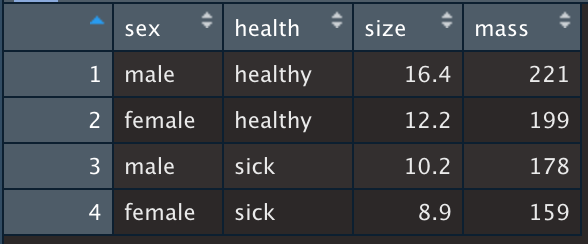
\includegraphics[width=0.5\linewidth]{images/dataframe} 

}

\caption{A view of the df data frame generated by the `View()` function.}\label{fig:df1}
\end{figure}

Each of the columns in the data frame contains one of the variables, with the name that we gave it when we created the data frame. We can access each of those columns using the \texttt{\$} operator. For example, if we wanted to access the size variable, we would combine the name of the data frame with the name of the variable as follows:

\begin{Shaded}
\begin{Highlighting}[]
\NormalTok{df}\SpecialCharTok{$}\NormalTok{size}
\end{Highlighting}
\end{Shaded}

\begin{verbatim}
## [1] 16.4 12.2 10.2  8.9
\end{verbatim}

This is just like any other vector, in that we can refer to its individual values using square brackets, as we did with regular vectors:

\begin{Shaded}
\begin{Highlighting}[]
\NormalTok{df}\SpecialCharTok{$}\NormalTok{size[}\DecValTok{3}\NormalTok{]}
\end{Highlighting}
\end{Shaded}

\begin{verbatim}
## [1] 10.2
\end{verbatim}

In reality, you will rarely have to build your own data frame in this class, because we will provide you will real data from classic studies and our own research that you can read into R. You will learn how to do that in \href{evidence-for-evolution.html\#import-data}{Chapter 2}.

\hypertarget{help-functions}{%
\subsubsection*{Help Functions}\label{help-functions}}
\addcontentsline{toc}{subsubsection}{Help Functions}

If you ever run into issues or have question regarding how to use a particular function or package, you can access the documentation with instruction using the question mark symbol (\texttt{?}) followed by the function or package name. For example, \texttt{?sqrt} will provide the instructions for the \texttt{sqrt()} function.

\hypertarget{additional-resources}{%
\section{Additional Resources}\label{additional-resources}}

\hypertarget{alternative-evolution-textbooks}{%
\subsection{Alternative Evolution Textbooks}\label{alternative-evolution-textbooks}}

If you would like more in-depth reading materials about evolution, there are a number of excellent textbooks available. I particularly recommend the edited volume by Losos et al.~with short articles about current topics in evolution, because it is freely available for online reading through most university libraries.

\begin{itemize}
\item
  Bergstrom CT, LA Dugatkin (2018): \href{https://wwnorton.com/books/Evolution/}{\emph{Evolution}}. Norton.
\item
  Emlen DJ, C Zimmer (2020): \href{https://www.macmillanlearning.com/college/us/product/Evolution/p/1319079865}{\emph{Evolution - Making Sense of Life}}. MacMillan.
\item
  Futuyma DJ, M Kirkpatrick (2017): \href{https://global.oup.com/ushe/product/evolution-9781605356051?cc=us\&lang=en\&}{\emph{Evolution}}. Oxford University Press.
\item
  Herron JC, S Freeman (2014): \href{https://www.pearson.com/us/higher-education/program/Herron-Evolutionary-Analysis-5th-Edition/PGM296285.html}{\emph{Evolutionary Analysis}}. Pearson.
\item
  Losos JB, DA Baum, DJ Futuyma, HE Hoekstra, RE Lenski, AJ Moore, CL Peichel, D Schluter, MC Whitlock (editors) (2014): \href{https://k-state-primo.hosted.exlibrisgroup.com/permalink/f/1aco38j/01KSU_ALMA51277244700002401}{\emph{The Princeton Guide to Evolution}}. Princeton University Press.
\end{itemize}

\hypertarget{evolution-in-the-primary-literature-and-the-news}{%
\subsection{Evolution in the Primary Literature and the News}\label{evolution-in-the-primary-literature-and-the-news}}

For some assignments, and to satisfy your innate curiosity, you may want to consider consulting other resources. You can browse through \href{http://evolution-textbook.org/content/free/notes/box_journal_list.html}{the list of peer-reviewed journals that publish research related to evolution}. If you want to find current research in the field, I also recommend the following websites, many of which provide lay summaries of recent papers:

\begin{itemize}
\item
  \href{https://www.eurekalert.org/}{EurekAlert!}
\item
  \href{https://www.nature.com/news}{Nature News}
\item
  \href{https://www.popsci.com/}{Popular Science}
\item
  \href{https://www.sciencedaily.com/}{Science Daily}
\item
  \href{https://www.sciencemag.org/news}{Science Magazine News}
\item
  \href{https://www.sciencenews.org/}{Science News}
\item
  \href{https://www.scientificamerican.com/}{Scientific American}
\end{itemize}

\hypertarget{r-and-rstudio-resources}{%
\subsection{R and RStudio Resources}\label{r-and-rstudio-resources}}

This book will provide you with the background knowledge necessary to use R at the level you need to succeed in this class. Nonetheless, you will run into issues, and being able to troubleshoot errors is one of the most important coding skills. \textbf{Perhaps the most important tool during troubleshooting is\ldots{} Google!} If you google your error message from R or specific questions you have, you will likely find that somebody else already had that problem. Question/answer threads associated with \href{https://stackoverflow.com/}{Stack Overflow} usually are a very reliable resource for overcoming issues with coding. If you need additional resources or want to dig a little deeper, consider the following:

\begin{itemize}
\item
  \href{https://www.oxfordscholarship.com/view/10.1093/acprof:oso/9780199601615.001.0001/acprof-9780199601615}{Getting Started with R: An Introduction for Biologists} (this may be worth it if you consider attending graduate school to earn a M.S. or Ph. D.)
\item
  The \href{http://www.sthda.com/english/}{Statistical Tools for High-Throughput Data Analysis} website has a number of fantastic R tutorials. The following may be helpful for you in this course:

  \begin{itemize}
  \item
    \href{http://www.sthda.com/english/wiki/r-basics-quick-and-easy}{Basic introduction to R and RStudio}
  \item
    \href{http://www.sthda.com/english/wiki/importing-data-into-r}{Import data into R}
  \item
    \href{http://r-statistics.co/ggplot2-Tutorial-With-R.html}{How to make any ggplot}
  \item
    \href{http://www.sthda.com/english/wiki/ggplot2-essentials}{Introduction to ggplot2}
  \item
    \href{http://www.sthda.com/english/wiki/ggplot2-barplots-quick-start-guide-r-software-and-data-visualization}{Bar plots with ggplot2}
  \item
    \href{http://www.sthda.com/english/wiki/ggplot2-histogram-plot-quick-start-guide-r-software-and-data-visualization}{Histogram plots with ggplot2}
  \item
    \href{http://www.sthda.com/english/wiki/ggplot2-scatter-plots-quick-start-guide-r-software-and-data-visualization}{Scatter plots with ggplot2}
  \item
    \href{http://www.sthda.com/english/wiki/ggplot2-box-plot-quick-start-guide-r-software-and-data-visualization}{Box plots with ggplot2}
  \end{itemize}
\end{itemize}

\hypertarget{reflection-questions}{%
\section{Reflection Questions}\label{reflection-questions}}

\begin{enumerate}
\def\labelenumi{\arabic{enumi}.}
\tightlist
\item
  How would you define evolution in your own words? How does your definition compare to the one given in this chapter? Are there other definitions of evolution? What are their strengths and weaknesses?
\item
  What is the difference between evolution and natural selection?
\item
  What do you think of the term ``survival of the fittest''? Is it an accurate description of evolution? If not, why?
\item
  Do you think evolution is a fact or a theory?
\item
  Darwin once wrote (1859): ``We see nothing of these slow changes in progress, until the hand of time has marked the lapse of ages.'' How long do you think it takes for evolution to take place?
\item
  While Darwin understood that some traits are inherited from parents to their offspring, he did not know exactly how that happens. He was largely unaware of the work of his contemporary, Gregor Mendel, who worked out the foundational principles of genetics. Instead Darwin hypothesized that the body continuously emitted small particles he called gemmules that accumulated in the gonads and contributed heritable information to the gametes. How do you think Darwin's misconceptions about heredity impacted the validity of his evolutionary ideas? How have discoveries in classical genetics and later the discovery of DNA carrying the genetic instructions for the development and functioning of all organisms strengthened or weakened our understanding of evolution as conceived by Darwin?
\item
  How does \href{https://en.wikipedia.org/wiki/Lamarckism}{Lamarck's view of evolution} differ from our current understanding? What aspects did he get right, and what did he get wrong?
\end{enumerate}

\hypertarget{references-1}{%
\section{References}\label{references-1}}

\begin{itemize}
\item
  Darwin, C. (1859). \emph{On the origin of species based on natural selection, or the preservation of favoured races in the struggle of life}. John Murray.
\item
  Darwin, C. (1868). \emph{The Variation of Animals and Plants under Domestication}. John Murray.
\item
  Darwin, C. (1889; original in 1839). \emph{Journal of Researches Into the Natural History and Geology of the Countries Visited During the Voyage of H.M.S. ``Beagle'' Round the World, Under the Command of Capt.~Fitz Roy}. Ward, Lock and Company.
\item
  Malik, A. H., Ziermann, J. M., \& Diogo, R. (2018). An untold story in biology: the historical continuity of evolutionary ideas of Muslim scholars from the 8th century to Darwin's time. \emph{Journal of Biological Education}, \emph{52}(1), 3--17.
\item
  Mayr E. 1982. The Growth of Biological Thought: Diversity, Evolution, and Inheritance. Cambridge (MA): Harvard University Press.
\end{itemize}

\hypertarget{evidence-for-evolution}{%
\chapter{Evidence for Evolution}\label{evidence-for-evolution}}

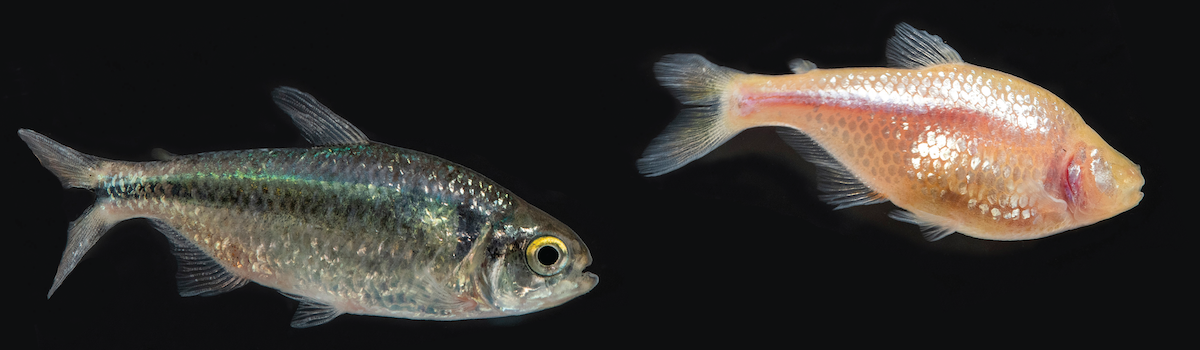
\includegraphics[width=1\linewidth]{images/chapter3_title}

Darwin described evolution as descent with modification. It turns out that he was not the only one to think about the ever-changing world in this way. Another prominent naturalist of the time, Alfred Russel Wallace, independently conceived the theory of evolution through natural selection. Like Darwin, Wallace conducted extensive fieldwork in the tropics and was a meticulous observer of the natural world. In 1858, Wallace wrote a letter to Darwin---who was by then an eminent scholar but had not published his views on evolution yet---detailing his own ideas about natural selection. This led to the joint publication of short abstracts detailing Darwin's and Wallace's views of evolution, and more importantly, it motivated Darwin to finish and publish his famous work, \emph{On the Origin of Species}, in 1859. So, why does most of the credit for formalizing evolutionary theory go to Darwin rather than Wallace? Well, Darwin was undoubtedly first, ruminating on his ideas about evolution for decades before deciding to publish. As a consequence, he was able to introduce his views in much richer detail and provided many lines of evidence in support of his theory.

Explore More

To learn more about Alfred Russel Wallace, listen to ``\href{https://www.npr.org/2013/04/30/177781424/he-helped-discover-evolution-and-then-became-extinct}{\emph{He Helped Discover Evolution, And Then Became Extinct}}'', an NPR story published on the 100\textsuperscript{th} anniversary of his death.

So, what evidence do we have that evolution is actually happening? What is the evidence for the occurrence of change in inherited traits across successive generations, the transformation of species through time, and the emergence of new species?

As mentioned in \href{what-evolution-is.html\#predictions}{Chapter 1}, we can (must!) treat Darwin's idea of descent with modification as every other scientific hypothesis and develop testable predictions that are falsifiable with data. The idea of descent with modification makes five predictions that we can address with data:

\begin{enumerate}
\def\labelenumi{\arabic{enumi}.}
\tightlist
\item
  Species change through time (microevolution).
\item
  Lineages split to form new species (speciation).
\item
  Novel forms derived from earlier forms (macroevolution).
\item
  Species are not independent but connected by descent from a common ancestor (common ancestry and homology).
\item
  Earth and life on Earth are old (deep time).
\end{enumerate}

This chapter takes a closer look at the different lines of evidence we have in support of evolution.

\hypertarget{microevolution}{%
\section{Microevolution}\label{microevolution}}

Microevolution is the change in inherited traits of a population from one generation to the next, ultimately leading to the accumulation of changes and the transformation of species through time. \emph{Heritable trait} in this context can refer to any phenotypic trait (for example the average beak size in a population of a bird) or a molecular trait (for example the frequency of alternative alleles at a particular locus). While changes in most traits from one generation to the next are subtle at best, strong natural selection can lead to significant and detectable evolutionary changes in very short periods of time. For example, check out the following video produced by the \href{https://kishony.technion.ac.il/}{Kishony Lab at Harvard Medical School}. They have designed a simple way to observe how bacteria evolve as they encounter increasingly higher doses of an antibiotic and adapt to survive---and thrive---despite of it.

You might say that bacteria are different. After all, assuming a generation time of 30 minutes, the two-week experiment described in the video represents over 670 generations of bacterial evolution. Translated to humans, that would represent about 17,000 years. Looking back that far in history, that was a time when humans exclusively lived as hunter-gatherers and just started to migrate into North America over the Bering Land Bridge\ldots{}

One of the most persistent misconceptions about evolution is that it takes millions of years to occur. However, the reality is that microevolution---in principle---can happen in as little as one generation. Those short-term changes can be very hard to detect, because our measurement error of a trait of interest is often larger than the actual per-generation evolutionary change. Nonetheless, over the course of just a handful of generations, natural populations may exhibit significant evolutionary change that we can detect with high confidence using genetic markers (\emph{i.e.}, measuring changes in allele frequencies) or phenotypic measurements.

The convergence of ecological and evolutionary timescales is a relatively recent insight. Darwin did not think that we would be able to directly observe evolutionary change over short periods of time:

\begin{quote}
``We see nothing of these slow changes in progress, until the hand of time has marked the lapse of ages.''

--- Darwin, 1859
\end{quote}

However, with technological breakthroughs that improved the precision of measurements we take in natural populations and with scientists' ability to track populations continuously through time, we have accumulated data across dozens of study systems---from microbes to vertebrates---documenting microevolutionary change within a few to a few dozen generations (see Hairston et al.~2005; Carroll et al.~2007). Here, I will briefly introduce you to evidence for rapid evolution gathered in one such study system (the threespine stickleback). In this chapter's case study, you will explore another example based on a time series of beak size variation of a species of Darwin's finch.

\hypertarget{the-case-of-threespine-stickleback}{%
\subsection{The Case of Threespine Stickleback}\label{the-case-of-threespine-stickleback}}

Threespine stickleback (\emph{Gasterosteus aculeatus}; Figure \ref{fig:stickleback}) are a widely used system to study evolution and have been shown to rapidly adapt to novel environmental conditions. Stickleback are primarily marine and inhabit coastal waters throughout much of the Northern hemisphere. They are small fish (usually less than 8 cm in length) that exhibit exquisite adaptations to avoid predation in their environment: the sides of their body are covered in bony plates, and they have spines associated with their dorsal and pelvic fins that, when spread out, can dissuade a predator from capturing or consuming them.

\begin{figure}
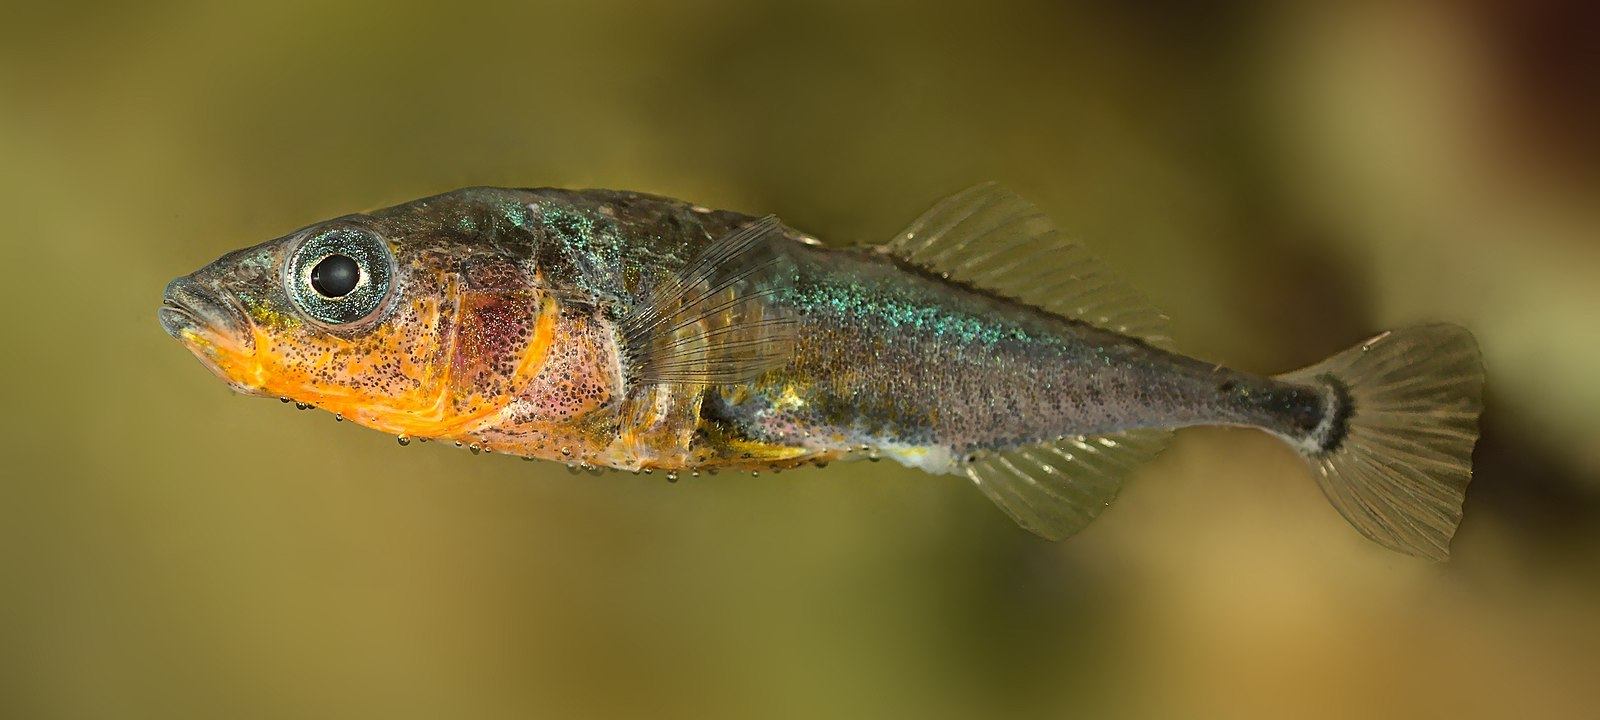
\includegraphics[width=1\linewidth]{images/Three-spined_stickleback} \caption{Threespine stickleback (*Gasterosteus aculeatus*). Photo by Gilles San Martin, [CC BY-SA 2.0](https://creativecommons.org/licenses/by-sa/2.0), via Wikimedia Commons}\label{fig:stickleback}
\end{figure}

Since the last ice age, as glaciers retreated and left behind a plethora of new streams and lakes, stickleback have also colonized freshwater habitats, which differ in many ways from the original marine habitats. Freshwaters not only exhibit a different water chemistry, but they also tend to harbor fewer predators and different food resources. Over the past 10,000-20,000 years, stickleback in freshwater environments have evolved a number of phenotypic differences compared to their marine ancestors, including a drastic reduction of the armor plates along the body and---in some instances---a loss of the pelvic spines (Jones et al.~2012). Moreover, stickleback have also adapted to different niches within freshwaters, and there are distinct morphs in streams and lakes, and in benthic and pelagic habitats within lakes (Hendry et al.~2013). Different freshwater ecotypes exhibit distinct body shapes and colorations and are adapted to consuming different types of prey items.

So, how long might it take for the evolution of the traits that vary so drastically across different stickleback forms? Sure, 20,000 years is a blink of an eye in the history of life on the planet, but it is still an eternity for any researcher that might want to observe evolution in action.

One hint at how fast stickleback might evolve comes from a fascinating natural experiment. In 1964, the Great Alaska Earthquake brought widespread destruction to the region and literally reshaped the regional topology. For example, multiple islands in the Prince William Sound and the Gulf of Alaska were lifted up further out of the ocean, creating new freshwater ponds where previously were none. In the time since the earthquake, stickleback have colonized these new freshwater ponds, and within just 50 years, they have evolved similar phenotypic traits that we know from stickleback in continental freshwaters (Lescak et al.~2015). Hence, adaptation to freshwaters upon colonization from the ocean may occur in a matter of a few decades rather than gradually over thousands of years of evolution.

To get a better understanding of just how fast evolution may proceed, researchers from the University of Basel in Switzerland decided to conduct a field experiment using lake and stream stickleback (Laurentino et al.~2020). The researchers first sequenced the genomes of lake and stream stickleback to detect the genomic regions that are differentiated between ecotypes and likely contain the genes involved in shaping the phenotypic differences between them. After that, they generated F2 crosses between the ecotypes, which is like shuffling a deck of cards from a genomic perspective: individual F2 offspring essentially exhibit a random mixture of genomic segments from their lake and stream ancestors. If these F2 hybrids were introduced into a stream environment, it is predicted that individuals that exhibit stream alleles in regions of the genome important for the expression of stream-specific phenotypic traits perform better than individuals with lake alleles. At a population level, this should lead to an increase in the frequency of alleles characteristic for stream stickleback. And, this is exactly what happened when the researchers actually conducted the experiment. More importantly, the predicted genetic changes were detectable within just one generation of F2 individuals being released into a stream habitat. So, when selection is strong and researchers have the capability to measure changes in traits with adequate precision, we can actually detect the small, generation-to-generation changes that ultimately accumulate to give rise to more conspicuous evolutionary changes that are easier to detect.

\hypertarget{speciation}{%
\section{Speciation}\label{speciation}}

Speciation is the process by which new species arise. Before we dive into how speciation actually works, we should agree on what species actually are:

Definition: Species

A \emph{biological species} is a group of organisms that can reproduce with one another in nature and produce fertile offspring. Species are characterized by the fact that they are reproductively isolated from other such groups, which means that the organisms in one species are incapable of reproducing with organisms in another species. (As you may know, there are alternative definitions of a species, which we will discuss in more detail in \href{speciation-1.html}{Chapter 11}.)

In phylogenetic trees, speciation is depicted as a singular point that represents the moment one lineage splits into two (red circle in Figure \ref{fig:speccont}). Although speciation can occur instantaneously, for example when polyploidization is involved (see \href{speciation-1.html}{Chapter 11}), new species typically evolve gradually, from a single variable population, to populations within a species that are differentiated but still connected through gene flow, to distinct species that are completely isolated from each other (Figure \ref{fig:speccont}). Movement along this ``speciation continuum'' is driven by the accumulation of reproductive barriers that prevent individuals from mating or successfully producing offspring with each other. Importantly, movement along the speciation continuum can be bidirectional, and reproductive barriers can disappear such that two species merge back together into one. If speciation is a gradual process, we should be able to observe all stages along the speciation continuum in nature, not just the endpoints of the speciation process with reproductively isolated species.

\begin{figure}
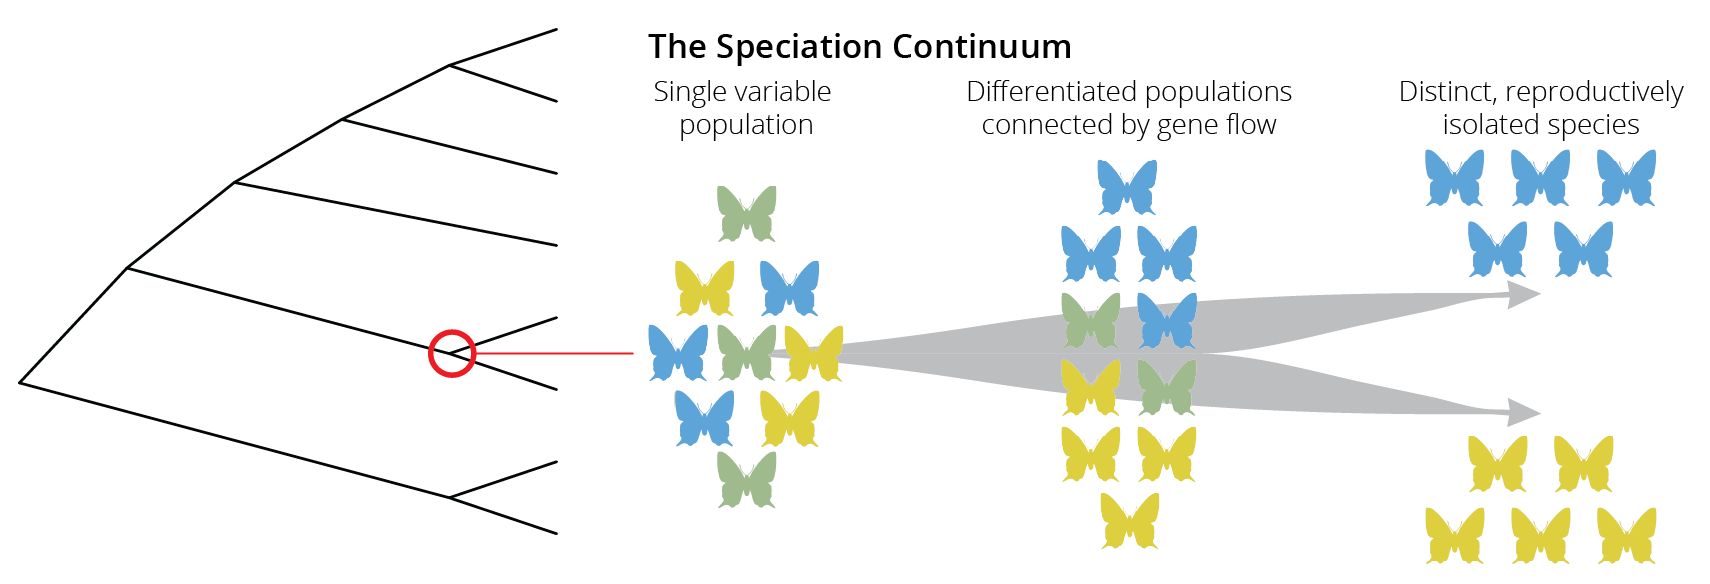
\includegraphics[width=1\linewidth]{images/speciation_continuum} \caption{Speciation is not typically an instantaneous process. Rather species evolve gradually along a speciation continuum.}\label{fig:speccont}
\end{figure}

\hypertarget{ring-species}{%
\subsection{Ring Species}\label{ring-species}}

One phenomenon that perfectly illustrates the speciation continuum and provides evidence for ongoing speciation are so-called ring species, in which two reproductively isolated populations living sympatrically (red and brown in Figure \ref{fig:ringspecies}) are connected by a geographic ring of populations that can interbreed. Such ring species arise when an original population disperses around a geographic barrier, and populations diverge gradually, for example as a consequence of adaptation to local environmental conditions. Once populations come into sympatry again behind the geographic barrier, sufficient differences have accumulated such that populations cannot interbreed with each other anymore.

\begin{figure}
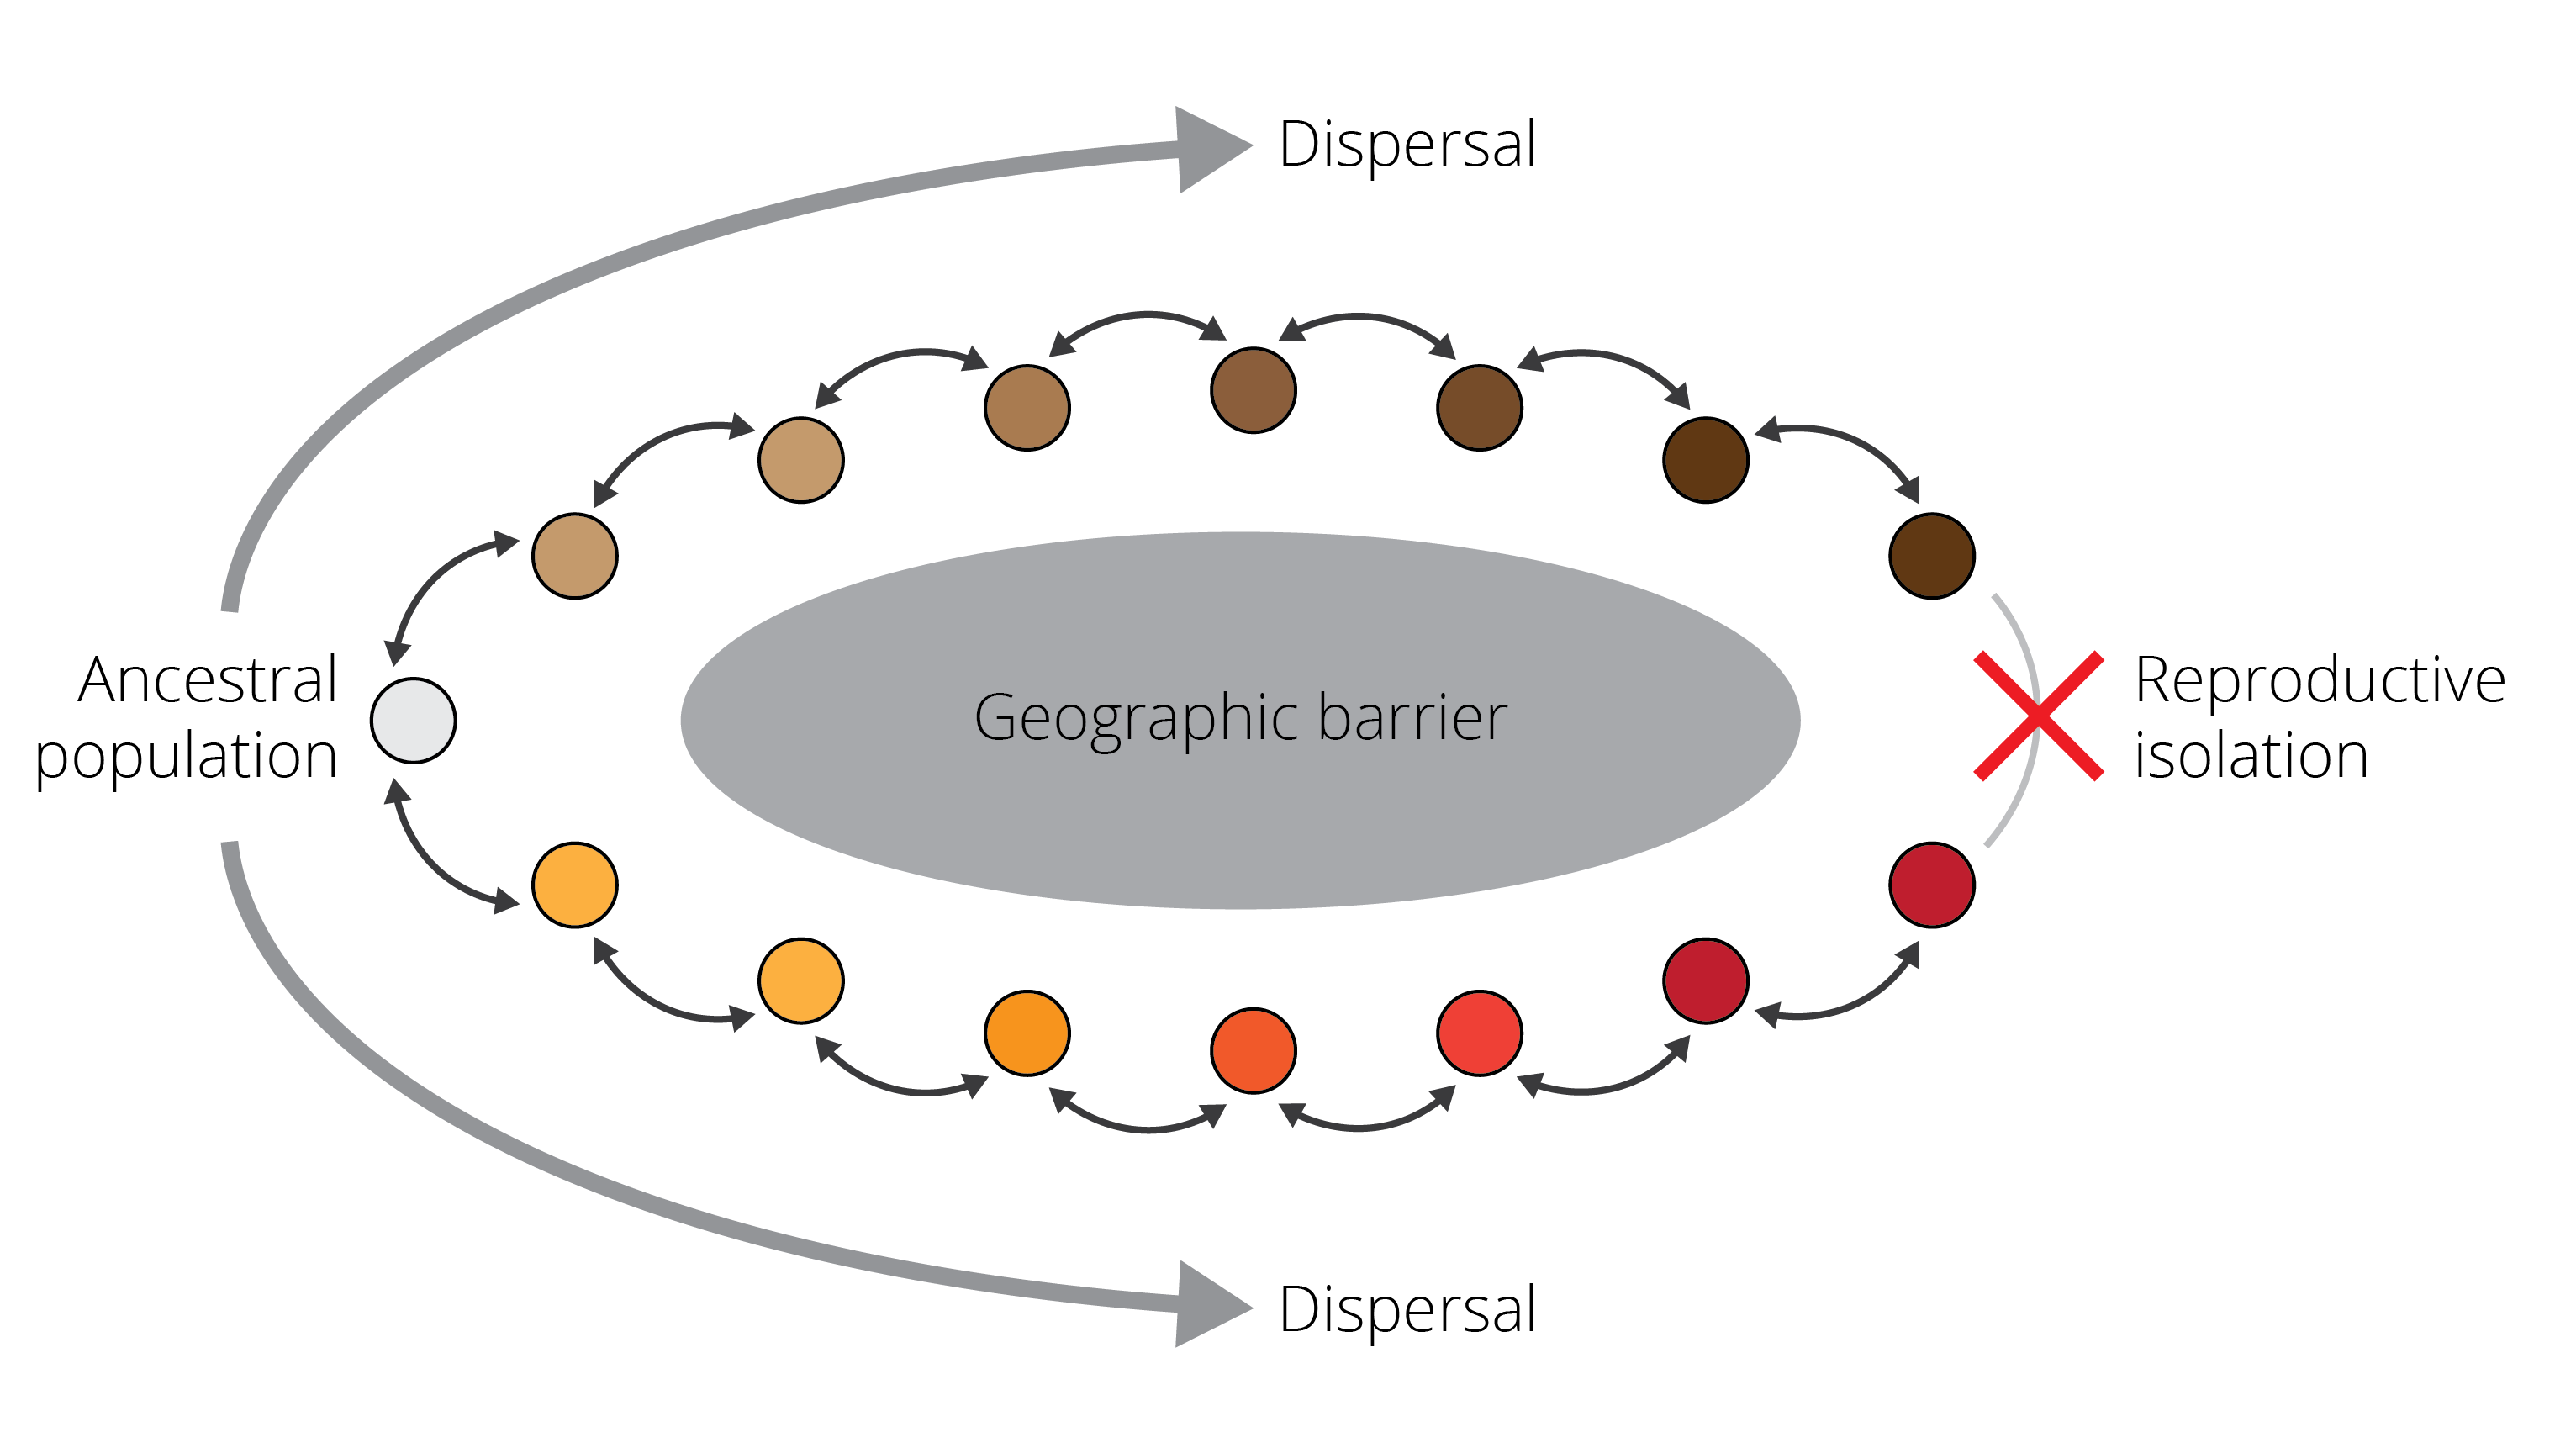
\includegraphics[width=1\linewidth]{images/rings-species} \caption{A schematic representing a ring species. Individuals are able to successfully reproduce with members of adjacent populations, as indicated by the black arrows. However, as populations disperse around a geographic barrier and diverge gradually, they are unable to reproduce when they come into contact again. This process represents a form of speciation occurring with gene flow.}\label{fig:ringspecies}
\end{figure}

Several well-studied examples of ring species exist. For example, plethodontid salamanders of the \emph{Ensatina eschscholtzii} complex have colonized different parts of California from the north and expanded southward around the Central Valley, which represents unsuitable habitat for salamanders. At the southern tip of the Central valley, salamander populations from the eastern and western mountain ridges that surround the valley came into secondary contact and are unable to interbreed due to the genetic changes that have accumulated during evolution in isolation (Pereira et al.~2011). Other examples of ring species include the herring and lesser black-backed gulls (genus \emph{Larus}) that have a circumpolar distribution and cannot interbreed in northern Europe. In addition, greenish warblers (\emph{Phylloscopus trochiloides}) form a ring species around the Himalayas (Irwin et al.~2005).

\hypertarget{catching-speciation-in-action}{%
\subsection{Catching Speciation in Action}\label{catching-speciation-in-action}}

Evidence for ongoing speciation also comes from a wide variety of study systems that do not occur in a ring. Especially when populations are subject to strong natural selection (for example if they inhabit different habitat types), we do not only observe adaptive differentiation across populations but also the inadvertent emergence of reproductive isolation. As populations acquire traits that make them better suited to the environments they inhabit, individuals also tend to stop interbreeding with individuals from different populations that have different traits. This is called ecological speciation, and we explore this concept in more detail in \href{speciation-1.html}{Chapter 11}. As a consequence, we can often find populations along various stages of the speciation continuum.

\emph{Timema} stick insects are a great example. These insects are distributed in the western United States, and different species of \emph{Timema} have adapted to live and feed on different host plants. While most species are uniformly green, gray, or brown and live on broad-leaved host plants, several species have independently evolved a dorsal stripe that provides camouflage on needle-like leaves, providing protection from predators (Figure \ref{fig:timema}). In at least one species, \emph{T. cristinae}, both uniformly colored and striped populations exist depending on whether they live on host plants with broad or needle-like leaves. While these phenotypic differences within \emph{T. cristinae} parallel differences between other \emph{Timema} species, reproductive isolation between different \emph{T. cristinae} populations utilizing alternative host plants is still incomplete (Nosil 2007). Hence, the different ecotypes represent intermediate stages of speciation. Similar variation along the speciation continuum has been uncovered in a wide variety of other natural study systems, and we will get to know some of them in more detail later in the book.

\begin{figure}
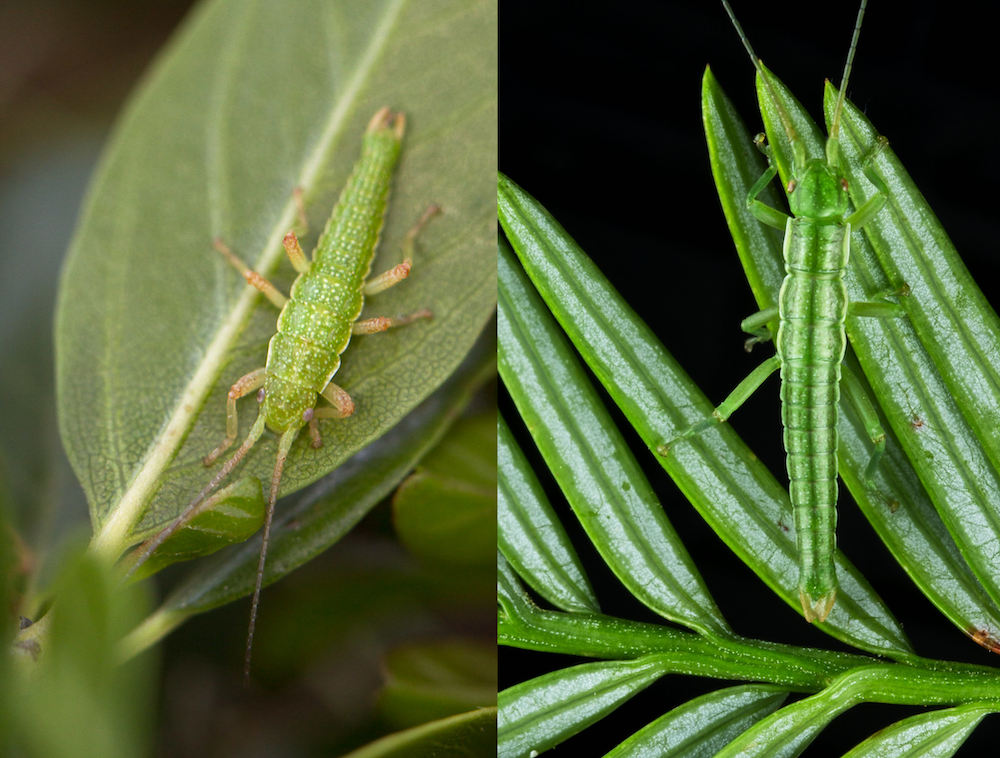
\includegraphics[width=1\linewidth]{images/timema} \caption{*Timema* stick insects have adapted to different host plants. Left: *T. cristinae* on one of its hosts, Greenbark (*Ceanothus spinosus*). Photo by [Aaron C](https://www.flickr.com/photos/90276319@N07/14165790793), [public domain](https://creativecommons.org/publicdomain/mark/1.0/). Right: *T. poppensis* on its host, Redwood (*Sequoia sempervirens*). Photo by [Moritz Muschick](https://www.flickr.com/photos/bmc_ecology/8592831488), [CC BY 2.0](https://creativecommons.org/licenses/by/2.0).}\label{fig:timema}
\end{figure}

\hypertarget{macroevolution}{%
\section{Macroevolution}\label{macroevolution}}

When discussing evidence for microevolution and speciation, we primarily turned to evidence from observations of living forms and from experiments. Here, we will consider a different type of evidence, fossils, which are simply the remains of prehistoric organisms. Fossils are usually petrified or preserved as a mold in rock, although the rapid thawing of permafrost accelerated by climate change has also revealed frozen fossils with amazing preservation of soft tissues (for example, check out \href{https://www.smithsonianmag.com/history/well-preserved-30000-year-old-baby-woolly-mammoth-emerges-from-yukon-permafrost-180980388/}{this story} about the recent discovery of nun cho ga, a baby woolly mammoth). The mere fact that fossils exist and often represent forms that are distinct from any organisms alive today (Figure \ref{fig:mammoth}) is testament to the ever-changing faunas and floras that have inhabited Earth through time. The fossil record also teaches us that extinction is an important aspect of evolutionary change, just as the generation of novel forms.

Explore More

If you are interested in learning more about what fossils teach us about evolution, I highly recommend Donald R. Prothero's book ``\href{https://cup.columbia.edu/book/evolution/9780231139625}{Evolution: What the Fossils Say and Why It Matters}''.

\begin{figure}
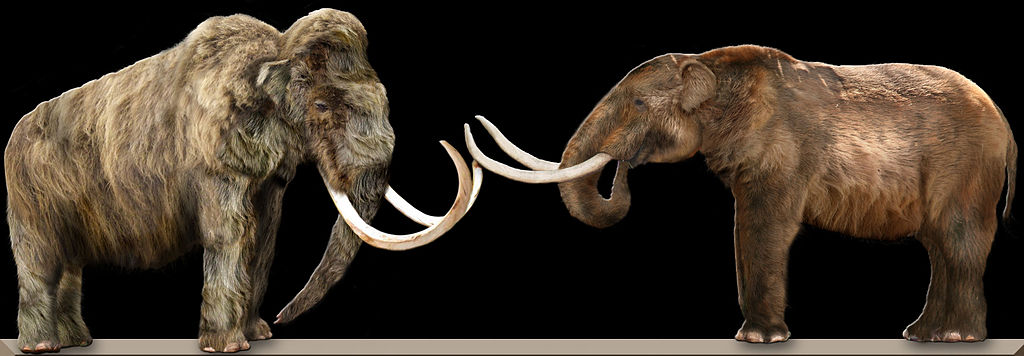
\includegraphics[width=1\linewidth]{images/MammothVsMastodon} \caption{A woolly mammoth (left) and an American mastodon (right) facing each other, showing the physical differences between the two extinct animals. Illustration by [Dantheman9758](https://en.wikipedia.org/wiki/User:Dantheman9758), [CC BY-SA 3.0](https://creativecommons.org/licenses/by-sa/3.0/deed.en).}\label{fig:mammoth}
\end{figure}

\hypertarget{geographic-and-temporal-patterns-of-succession}{%
\subsection{Geographic and Temporal Patterns of Succession}\label{geographic-and-temporal-patterns-of-succession}}

Perhaps the strongest evidence fossils provide for Darwin's notion of evolution is that they are not randomly distributed, neither in terms of geography nor time. The constant cycle of descent with modification and extinction has created predictable patterns in fossil deposits across the planet, which is evident as a succession of novel forms that are derived from earlier ones.

Patterns of succession are evident geographically, because there tends to be a regional correspondence between fossils and living forms. That is, we tend to find fossil relatives of extant species in the same areas where extant species live today. For example, marsupial fossils are particularly common in Australia just like living marsupials today. This is also reflected in the biogeographic distribution of extant forms, which frequently tracks the changing landmasses driven by continental drift. Marsupials are not only found in Australia but also South America, which were once connected through Antarctica in a large landmass called Gondwana until about 140 million years ago. The non-random distribution of fossils means that we can develop hypotheses and test predictions about the fossil record. For example, if the biogeographic distribution of marsupials was the consequence of a once contiguous distribution on Gondwana, we would predict the presence of marsupial fossils on Antarctica, which have indeed been found (Woodburne \& Zinsmeister 1982).

Patterns of succession are also evident temporally, with fossils exhibiting more ancestral traits being found in older layers of rock compared to derived forms. Subsequently deposited rock layers can therefore shed light into the temporal dynamics of trait evolution and reveal entire time series that connect forms with disparate phenotypes. For example, we know that horses with their single hoof descended from multi-toed ancestors, because we have a time series of horse fossils that illustrates the toe reductions through time (Figure \ref{fig:horse}).

\begin{figure}
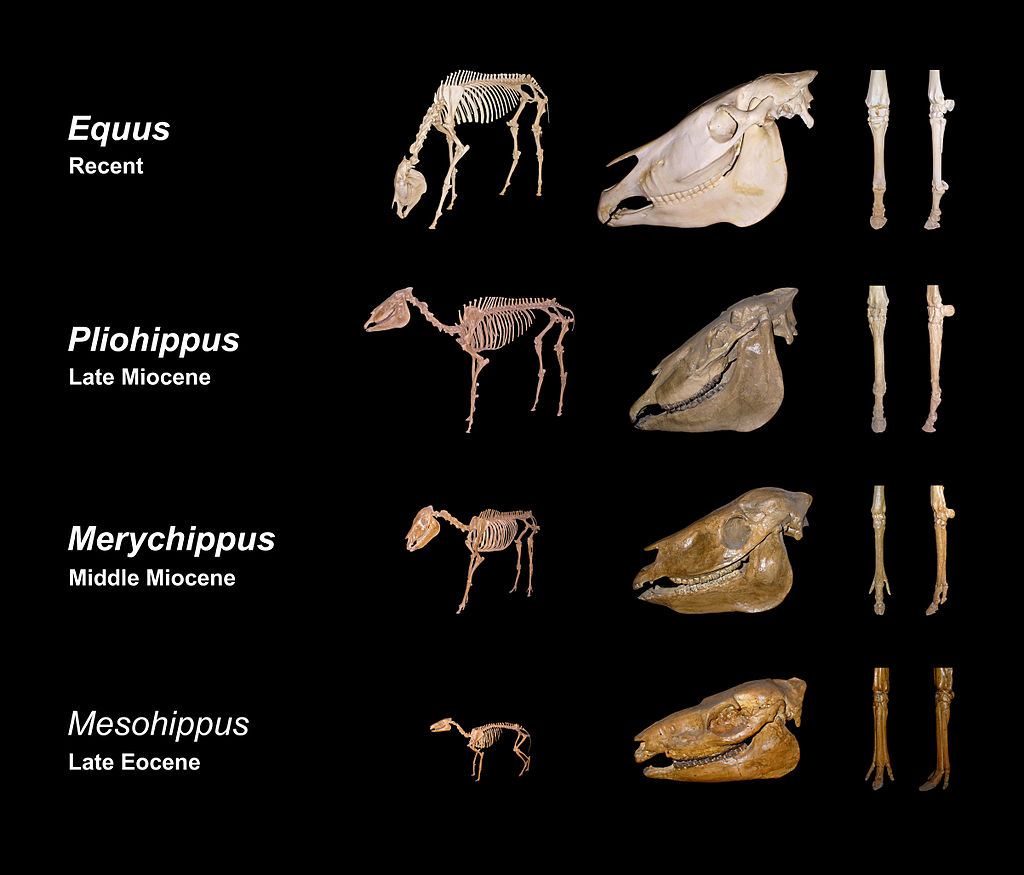
\includegraphics[width=1\linewidth]{images/Equine_evolution} \caption{Equine evolution, composed from skeletons of the State Museum for Natural History Karlsruhe, Germany. From left to right: Size development, biometrical changes in the cranium, reduction of toes on the left forefoot. Image by H. Zell, [CC BY-SA 3.0](https://creativecommons.org/licenses/by-sa/3.0), via Wikimedia Commons.}\label{fig:horse}
\end{figure}

\hypertarget{transitional-fossils}{%
\subsection{Transitional Fossils}\label{transitional-fossils}}

If novel forms are indeed descendants from earlier forms, the fossil record should capture evidence of what Darwin called the ``transmutation of species''. Hence, we should be able to find transitional fossils that exhibit traits common to both an ancestral group and its derived descendants. The first, and perhaps still one of the most spectacular, transitional fossil ever found was \emph{Archaeopterix} (Figure \ref{fig:archaeopteryx}), which shared traits with Mesozoic dinosaurs and modern birds. Its jaws contained sharp teeth, and it has wings with fingers and claws, a long bony tail, hyperextensible second toes (like \emph{Velociraptor}'s), and feathers. Hence, \emph{Archaeopterix} represents a transitional fossil between modern birds and non-avian dinosaurs (Ostrom 1976). Similar transitional fossils have been discovered to link the transition from aquatic to terrestrial vertebrates (\protect\hyperlink{tiktaalik}{\emph{Tiktaalik}}), from marine mammals to their terrestrial ancestors (\emph{Pakicetus}, \emph{Ambulocetus}, and \emph{Remingtonocetus}), and from quadrupedal to bipedal hominids (\href{human-origins-and-human-mediated-evolution.html}{\emph{Australopithecus afarensis}}), among many others.

\begin{figure}
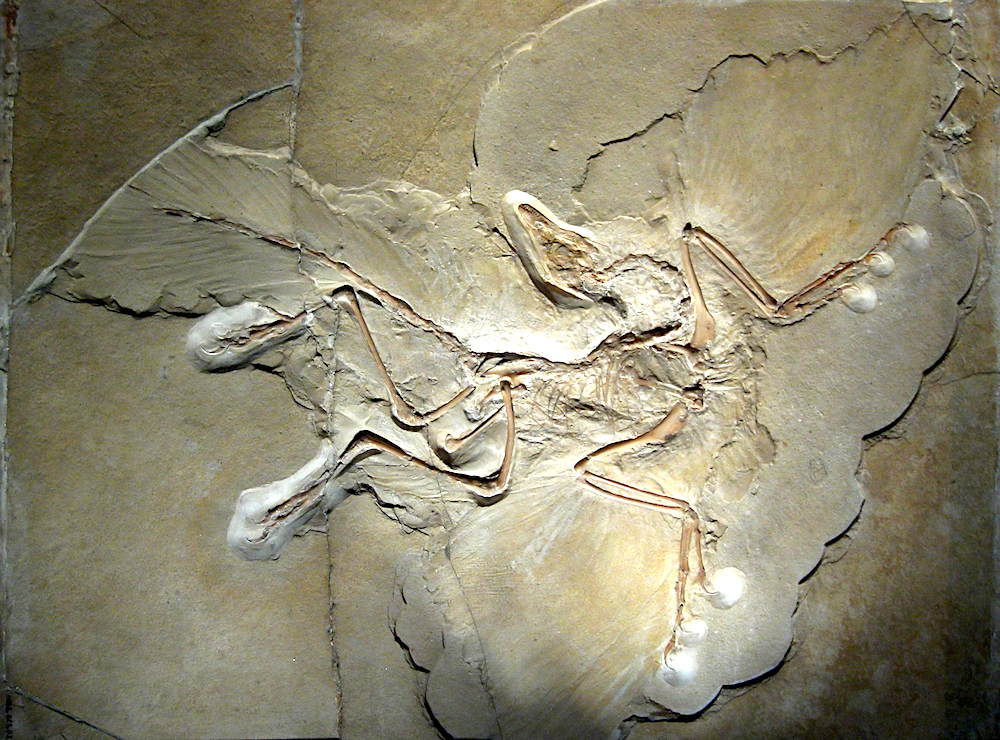
\includegraphics[width=1\linewidth]{images/Archaeopteryx_lithographica} \caption{*Archaeopteryx lithographica*, specimen displayed at the Museum of Natural History, Berlin, Germany. Photo by H. Raab, [CC BY-SA 3.0](https://creativecommons.org/licenses/by-sa/3.0/deed.en), via Wikimedia Commons.}\label{fig:archaeopteryx}
\end{figure}

\hypertarget{common-ancestry-and-homology}{%
\section{Common Ancestry and Homology}\label{common-ancestry-and-homology}}

A key prediction of Darwin's notion of evolution is that species are not independent but connected by descent from a common ancestor. Phylogenetic trees (Figure \ref{fig:ithink}) are representations of that connectedness, and if we were to travel back in time toward the root of the phylogenetic tree, we would expect lineages to merge into the origin of life, the original being from which all living forms descended (also known as the last universal common ancestor, or LUCA). In the absence of time travel, the critical evidence for common ancestry of all life is homology.

Definition: Homology

Homology is the similarity of the structure, physiology, or development of different species based upon their descent from a common evolutionary ancestor.

\begin{figure}
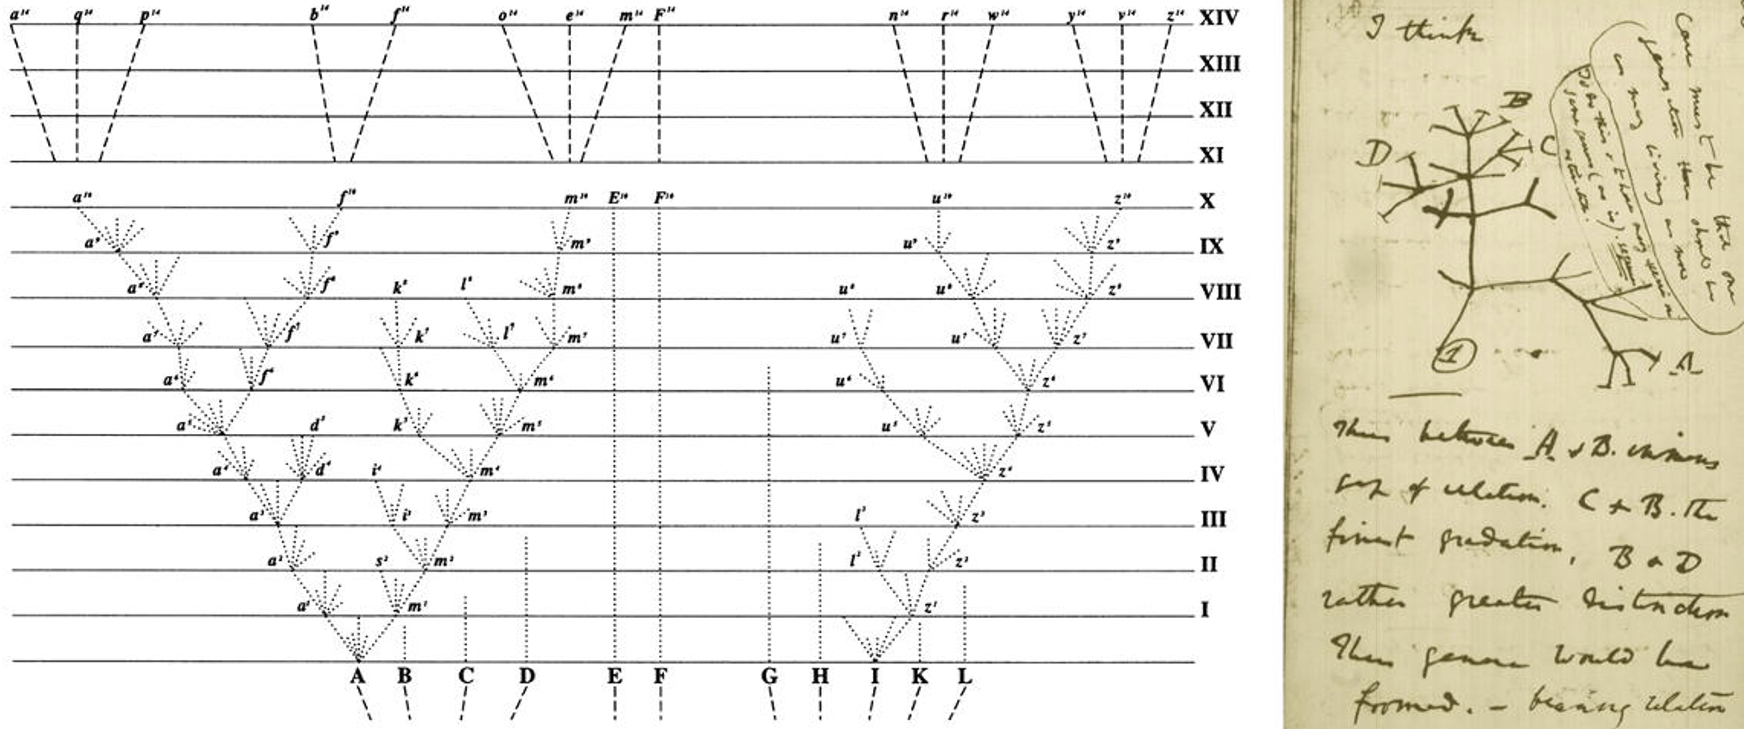
\includegraphics[width=1\linewidth]{images/I_think} \caption{The original phylogenetic trees Darwin used to illustrate common ancestry. Left: The Tree of Life image that appeared in Darwin's *On the Origin of Species by Natural Selection* (1859). It was the book's only illustration. Right: Charles Darwin's original 1837 sketch, his first diagram of an evolutionary tree from his *First Notebook on Transmutation of Species* (1837). Illustrations by Charles Darwin, [Public Domain](https://creativecommons.org/publicdomain/zero/1.0/).}\label{fig:ithink}
\end{figure}

Homology explains why all forms of life share certain characteristics. All forms of life, from microbes to plants and animals, share the same molecular building blocks: lipids that form the boundaries of cells and organelles, nucleic acids that encode information, proteins that play both structural and catalytic roles, and glycans that serve structure, energy storage, and regulatory purposes (Marth 2008). Different life forms, even those separated by billions of years of evolution, share these building blocks because they inherited them from a common ancestor.

Homologies also occur at a more narrow scope. For example, Darwin was puzzled by the structural similarity in the forelimbs of terrestrial vertebrates even though they serve entirely different functions (Figure \ref{fig:homology}):

\begin{quote}
What could be more curious than that the hand of a man, formed for grasping, that of a mole for digging, the leg of a horse, the paddle of the porpoise, and the wing of a bat, should all be constructed on the same patterns, and should include the same bones, in the same relative position?

--- Darwin, 1859
\end{quote}

How do these similarities in structure arise? Again, it is because all terrestrial vertebrates inherited this shared limb structure from their common ancestor. Rather than ``inventing'' different types of forelimbs for different purposes (grabbing, running, flying, swimming), evolution has gradually modified and repurposed existing forelimb structures for new functions.

\begin{figure}
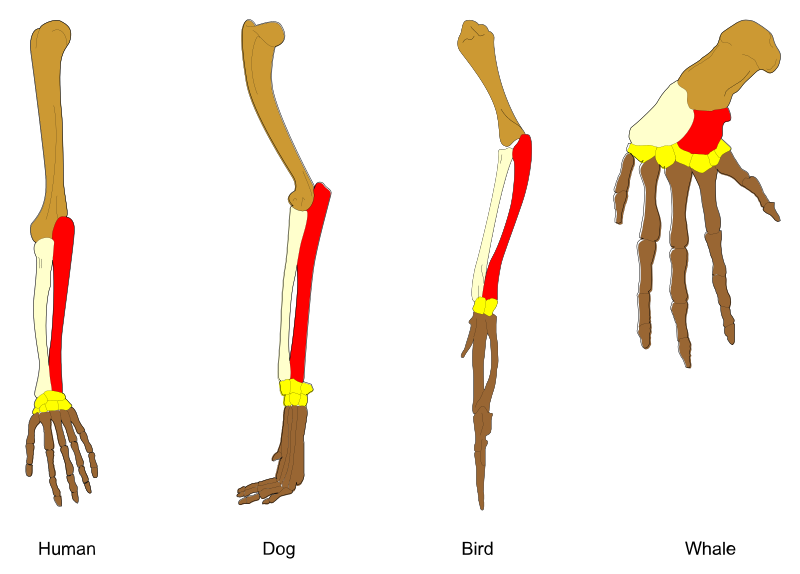
\includegraphics[width=1\linewidth]{images/homology} \caption{Limbs of terrerstrial vertebrates exhibit the same structure, with homologous bones  (color-coded) that are arranged in the same order irrespective of function. Illustration by Волков Владислав Петрович, [CC BY-SA 4.0](https://creativecommons.org/licenses/by-sa/4.0), via Wikimedia Commons.}\label{fig:homology}
\end{figure}

Homologies occur in nested sets. Closely related species exhibit a higher number of homologies, because they inherited those traits from a shared ancestor. More distantly related taxa exhibit differences in their traits, because they have been on independent evolutionary trajectories for prolonged periods of time. Accordingly, analyses of homologous structures are used to infer phylogenetic relationships among taxa. We group species that share a lot of homologous traits closely together on a phylogenetic tree, while those that share few are further apart (see \href{molecular-evolution.html}{Chapter 7} for more information).


\includegraphics[width=0.20833in,height=\textheight]{images/important.png} \textbf{Important Note}

Not all trait similarities are the consequence of homology. \textbf{Analogy} in biology describes similarity of function and superficial resemblance of structures that have different origins. For example, the wings of a fly, a moth, and a bird are analogous, because they evolved independently as adaptations to a common function (flying). Analogies are a consequence of convergent evolution, where unrelated lineages evolve similar traits, typically as adaptations to similar lifestyles or environmental conditions.

\hypertarget{shared-flaws}{%
\subsection{Shared Flaws}\label{shared-flaws}}

Perhaps the most compelling evidence for common ancestry comes from homologous structures that serve no purpose at all. The origin of these structures cannot be explained by adaptive evolution, and the only reason that some organisms exhibit functionless structures is because they have inherited them from an ancestor. I want to briefly introduce two such cases, vestigial organs and pseudogenes.

\hypertarget{vestigial-organs}{%
\subsubsection*{Vestigial Organs}\label{vestigial-organs}}
\addcontentsline{toc}{subsubsection}{Vestigial Organs}

Vestigial organs are rudimentary traits that lost some or all of the ancestral functions of the structure. Classic examples of vestigial organs in humans are the appendix (vestigial caecum), the coccyx (vestigial tail), and some muscles connected to the ear, which allow for ear mobility in other primates. Structural vestigial organs in other animals include remnants of limbs that are still expressed in some whales, snakes, and flightless birds (Figure \ref{fig:vestigial}).

\begin{figure}
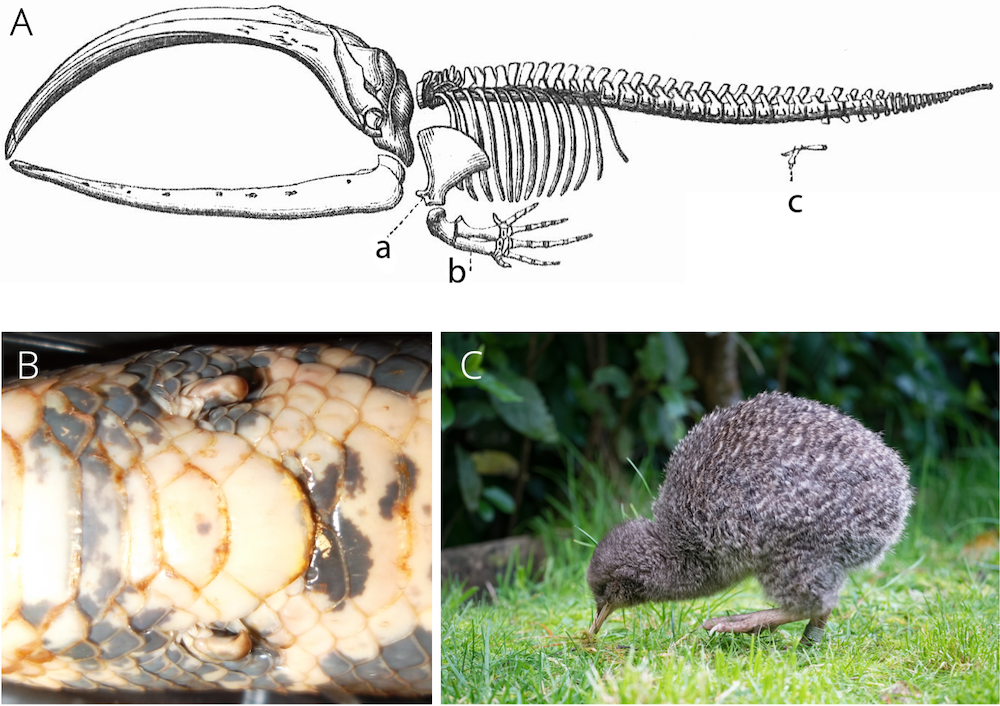
\includegraphics[width=1\linewidth]{images/vestigial} \caption{Vestigial limbs are common in tetrapods. A. Skeleton of a baleen whale showing the vestigial hindlegs (structure c). Illustration from Meyers Konversionlexikon, [Public Domain](https://creativecommons.org/publicdomain/zero/1.0/). B. Vestigial hindlegs (spurs) in a *Boa constrictor*. Photo by Stefan3345, [CC BY-SA 4.0](https://creativecommons.org/licenses/by-sa/4.0). C. Little spotted kiwi (*Apteryx owenii*) have vestigial wings that are completely invisible below the plumage. Photo by Judi Lapsley Miller, [CC BY 4.0](https://creativecommons.org/licenses/by/4.0).}\label{fig:vestigial}
\end{figure}

One of the most fascinating examples of vestigiality comes from Mexican cavefish (\emph{Astyanax mexicanus}) that are eyeless and completely blind as adults (Figure \ref{fig:astyanax}). Cavefish actually start growing eyes during embryonic development, and the lack of eyes in adult fish is a consequence of the abortion of eye development within the first few days of the growing embryo. The eye in this case is a developmental (rather than a structural) vestigial organ that makes a transient appearance during certain embryonic stages. More importantly, cavefish actually possess all the genes required for the normal development of an eye. It turns out, eye abortion is initiated by signaling factors associated with the developing cavefish lens. Transplantation of a surface fish lens into a developing cavefish leads to the normal formation of an eye, just like transplantation of a cave fish lens into a surface fish embryo leads to eye abortion (Krishnan and Rohner 2017). If cavefish had originated independently, there would be no need for evolution to ``create'' the developmental machinery for eye development. Cavefish have that machinery because they lost eyes secondarily and inherited all the information for making an eye from their eyed surface ancestors.

\begin{figure}
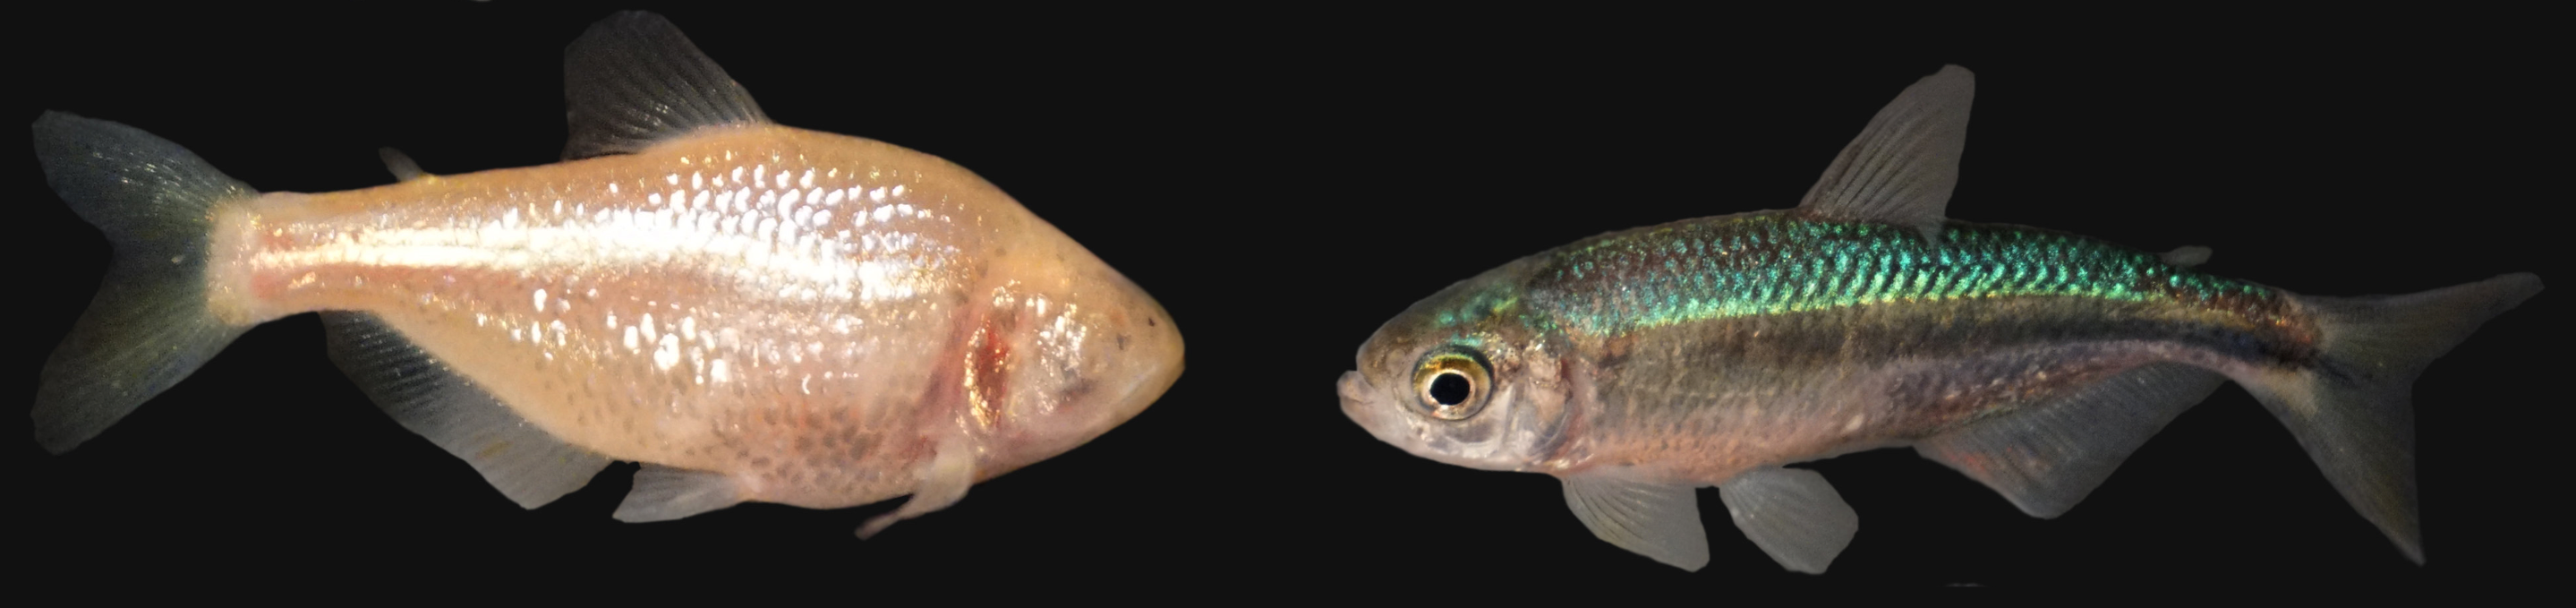
\includegraphics[width=1\linewidth]{images/astyanax} \caption{Different forms of *Astyanax mexicanus*. Left: Cave form, which is completely blind and lacks body pigmentation as an adult. Right: An individual from a surface stream for comparison. Photos by [Daniel Castranova, NICHD/NIH](https://www.flickr.com/photos/nihgov/27589386037), [Public Domain](https://creativecommons.org/share-your-work/public-domain/).}\label{fig:astyanax}
\end{figure}

\hypertarget{pseudogenes}{%
\subsubsection*{Pseudogenes}\label{pseudogenes}}
\addcontentsline{toc}{subsubsection}{Pseudogenes}

Pseudogenes are inactive copies of functional genes in the genome and represent another kind of evolutionary ``flaw''. Pseudogenes arise when processed messenger RNA (mRNA) is reverse-transcribed and inserted back into the genome. Reverse transcription is typically associated with retrotransposons or the activity of retroviruses in cells. Because processed mRNAs lack introns and other genetic elements important for transcription and translation, the complimentary DNA (cDNA) that is built back into the genome ends up being functionless. Hence, pseudogenes essentially represent junk DNA invisible not only to the cellular machinery responsible for protein synthesis, but for natural selection as well.

The reason that pseudogenes are invisible for natural selection is that they make no contribution to the phenotype of an organism, neither good or bad. While copy mistakes (\emph{i.e.}, mutations) that impair the function of normal genes are usually eliminated by selection, similar mutations in pseudogenes have no effect and just linger around. As generations pass, pseudogenes consequently tend to accumulate more and more mutations compared to the original functional gene they originated from. Since mutations in the genome occur at predictable rates, we can compare pseudogenes to their functional equivalents to estimate when pseudogenes first arose. Conducting such analyses for pseudogenes in the human genome revealed that some of them are really old---much older in fact than the human species. This suggests that those pseudogenes must have arisen in an ancient ancestor, which we share with other closely related species. If this is the case, we should be able to find the same pseudogenes in other primates, but only those that have diverged from a common ancestor after the origin of the pseudogene.

Friedberg and Rhoads (2000) put this hypothesis to the test (Table 2.1). The oldest pseudogene they investigated (CALM II 𝛙\textsubscript{3}), which has an estimated age of about 36 million years (Myr) based on the mutational difference from the functional equivalent, is found in all five species of primates that they investigated (including divergence times between 8 and 36 Myr). In contrast, the youngest pseudogene (𝛂-Enolase 𝛙\textsubscript{1}; 11 Myr old) is only found in chimpanzees and gorillas, the only primates that have diverged from the human lineage less than 11 Myr ago. Overall, the pattern of the presence and absence of pseudogenes is consistent with common ancestry. There is no reason for species to evolve the same pseudogenes independently in a predictable pattern. Rather, species share these ``flaws'' simply because they were passed down from one generation to the next, even as lineages split and formed new species.

\begin{longtable}[]{@{}
  >{\raggedright\arraybackslash}p{(\columnwidth - 12\tabcolsep) * \real{0.2717}}
  >{\centering\arraybackslash}p{(\columnwidth - 12\tabcolsep) * \real{0.1413}}
  >{\centering\arraybackslash}p{(\columnwidth - 12\tabcolsep) * \real{0.1087}}
  >{\centering\arraybackslash}p{(\columnwidth - 12\tabcolsep) * \real{0.1304}}
  >{\centering\arraybackslash}p{(\columnwidth - 12\tabcolsep) * \real{0.1087}}
  >{\centering\arraybackslash}p{(\columnwidth - 12\tabcolsep) * \real{0.1196}}
  >{\centering\arraybackslash}p{(\columnwidth - 12\tabcolsep) * \real{0.1196}}@{}}
\caption{Table 2.1: Pseudogenes that Friedberg and Rhoads (2000) detected in different primates (with hamsters as an outgroup). Individual pseudogenes identified in the human genome, along with their age estimates, are listed in rows. Different species with their estimated divergence times from humans are in columns. Symbols indicat the presence (+) or absence (-) of specific pseudogenes in a particular species.}\tabularnewline
\toprule
\begin{minipage}[b]{\linewidth}\raggedright
\end{minipage} & \begin{minipage}[b]{\linewidth}\centering
Chimpanzee
\end{minipage} & \begin{minipage}[b]{\linewidth}\centering
Gorilla
\end{minipage} & \begin{minipage}[b]{\linewidth}\centering
Orangutan
\end{minipage} & \begin{minipage}[b]{\linewidth}\centering
Rhesus
\end{minipage} & \begin{minipage}[b]{\linewidth}\centering
Capuchin
\end{minipage} & \begin{minipage}[b]{\linewidth}\centering
Hamster
\end{minipage} \\
\midrule
\endfirsthead
\toprule
\begin{minipage}[b]{\linewidth}\raggedright
\end{minipage} & \begin{minipage}[b]{\linewidth}\centering
Chimpanzee
\end{minipage} & \begin{minipage}[b]{\linewidth}\centering
Gorilla
\end{minipage} & \begin{minipage}[b]{\linewidth}\centering
Orangutan
\end{minipage} & \begin{minipage}[b]{\linewidth}\centering
Rhesus
\end{minipage} & \begin{minipage}[b]{\linewidth}\centering
Capuchin
\end{minipage} & \begin{minipage}[b]{\linewidth}\centering
Hamster
\end{minipage} \\
\midrule
\endhead
& 8 Myr & 9 Myr & 16 Myr & 25 Myr & 36 Myr & \textgreater85 Myr \\
\textbf{𝛂-Enolase} 𝛙\textsubscript{\textbf{1}}

11 Myr & + & + & - & - & - & - \\
\textbf{AS} 𝛙\textbf{7}

16 Myr & + & - & + & - & - & - \\
\textbf{CALM II} 𝛙\textsubscript{\textbf{2}}

19 Myr & + & + & + & - & - & - \\
\textbf{AS} 𝛙\textsubscript{\textbf{1}}

25 Myr & + & + & + & + & - & - \\
\textbf{AS} 𝛙\textsubscript{\textbf{3}}

25 Myr & + & + & + & + & - & - \\
\textbf{CALM II} 𝛙\textsubscript{\textbf{3}}

36 Myr & + & + & + & + & + & - \\
\bottomrule
\end{longtable}

\hypertarget{why-homologies-matter}{%
\subsection{Why Homologies Matter}\label{why-homologies-matter}}

The fact that evolutionary novelties occur in nested sets as predicted by descent with modification provides strong evidence for common ancestry. The finding also has far reaching implications, because it underlies all biomedical research and applications. The reason we can study DNA repair mechanisms in bacteria to learn about their role in cancer development is because DNA repair mechanisms in bacteria and humans are homologous. The reason we can study cell cycle regulation in yeast is because both yeast and humans inherited the same regulatory machinery from a common ancestor. The reason we can study drug responses in rodents is because the physiological processing of many substances is mediated by homologous pathways in rodents and humans. And we can gain insights about neurophysiology and psychiatry from other primates, again because we all inherited our neurosystem from a common ancestor. The reason evolution is the unifying theory of biology is because it provides the critical framework for comparative studies among species, helping us to make sure that we are actually comparing apples to apples (\emph{i.e.}, homologous structures). If not, inferences from comparative analyses can be deeply flawed.

\hypertarget{deep-time}{%
\section{Deep Time}\label{deep-time}}

The last prediction of Darwin's idea of descent with modification is that Earth and life on it are old. The study of the age of Earth and the universe is not really a subject of biology (hence, I will only touch on this briefly). The age of Earth is chiefly studied by geologists who combine isotopic analyses with an understanding of radioactive decay (radiometric dating), and they have established that Earth is about 4.54 billion years old (see \href{https://www.scientificamerican.com/article/how-science-figured-out-the-age-of-the-earth/}{Paul Braterman's article in \emph{Scientific American}} if you want more information). Similarly, astronomers have estimated the age of the universe at 13.8 billion years by measuring the rate of expansion of the universe and extrapolating back to the Big Bang (see \href{https://www.forbes.com/sites/startswithabang/2019/12/10/this-is-how-astronomers-know-the-age-of-the-universe-and-you-can-too/?sh=31f9137d16d5}{Ethan Siegel's article in \emph{Forbes}}). Evidence for the age of life on Earth comes unsurprisingly from the fossil record. The oldest known fossils are cyanobacteria found in Australian rock formations. Radiometric dating has revealed that they are 3.5 billion years old. Hence, all evidence indicates that life on Earth has had incredibly long periods of time to evolve and create the diversity of organisms observable today.

\hypertarget{tiktaalik}{%
\section{Correspondence of Different Lines of Evidence}\label{tiktaalik}}

Inference in science is strongest when there is a clear correspondence between different lines of evidence that all support a central hypothesis (consilience). In fact, we can often use existing information to formulate testable hypotheses that then can be addressed with alternative approaches. You have have already learned about one such example in the context of pseudogenes. Estimating the age of pseudogenes by tallying the number of mutations between a pseudogene and its functional equivalent led to clear predictions about the phylogenetic distribution of pseudogenes to test for common ancestry.

The discovery of \emph{Tiktaalik}, a transitional fossil between aquatic and terrestrial vertebrates discovered by a research team around Neil Shubin (Figure \ref{fig:tiktaalik}), is another example for the role of interdisciplinary research in making discoveries that transform our understanding. \emph{Tiktaalik} was not discovered haphazardly by a bunch of rock-loving paleontologists that were just looking for fossils. Its discovery was deliberate and testimony to the power of the scientific method. Wanting to find a transitional fossil that exhibited characteristics of both fish and early tetrapods, Shubin and his team first turned to molecular phylogenetic analyses of vertebrates. Essentially, they used DNA sequences to not only infer the evolutionary relationships between different vertebrate groups but also to date when different lineages split from each other (we will learn exactly how this works in \href{molecular-evolution.html}{Chapter 7}). These analyses revealed that terrestrial vertebrates (Tetrapoda) are sister to the lungfishes (Dipnoi), a lineage from which they split between 350-425 million years ago (Figure \ref{fig:vertphylo}). Any transitional fossils that exhibit traits intermediate between the two groups should consequently be found in rock layers of about that age. Accordingly, Shubin and colleagues took out a geological map of Earth in search of exposed rock formations of the correct age range, and they found some on Ellesmere Island in the Nunavut Territory of Canada. After a few disappointing field seasons, Shubin and his team indeed found a fossil with the predicted combination of traits in 2004. \emph{Tiktaalik roseae}, as they named the newly discovered species, exhibited gills and scales like fish but also limb bones characteristic of today's land animals (Daeschler et al.~2006). It's the combination of multiple approaches rooted in molecular biology, evolutionary analyses, and paleontology that ultimately led to the discovery of this missing link. Looking for corresponding evidence from different research approaches leads to the most robust inference in science, an approach frequently used in evolutionary biology.

Explore More

If you want to learn more about the fascinating discovery of Tiktaalik and its implications for evolution and our own origins, I recommend you either read Neil Shubin's book ``\href{https://www.amazon.com/Your-Inner-Fish-Journey-3-5-Billion-Year/dp/0307277453}{\emph{Your Inner Fish}}'' or watch the \href{https://www.pbs.org/your-inner-fish/}{PBS series based on the book}.

\begin{figure}
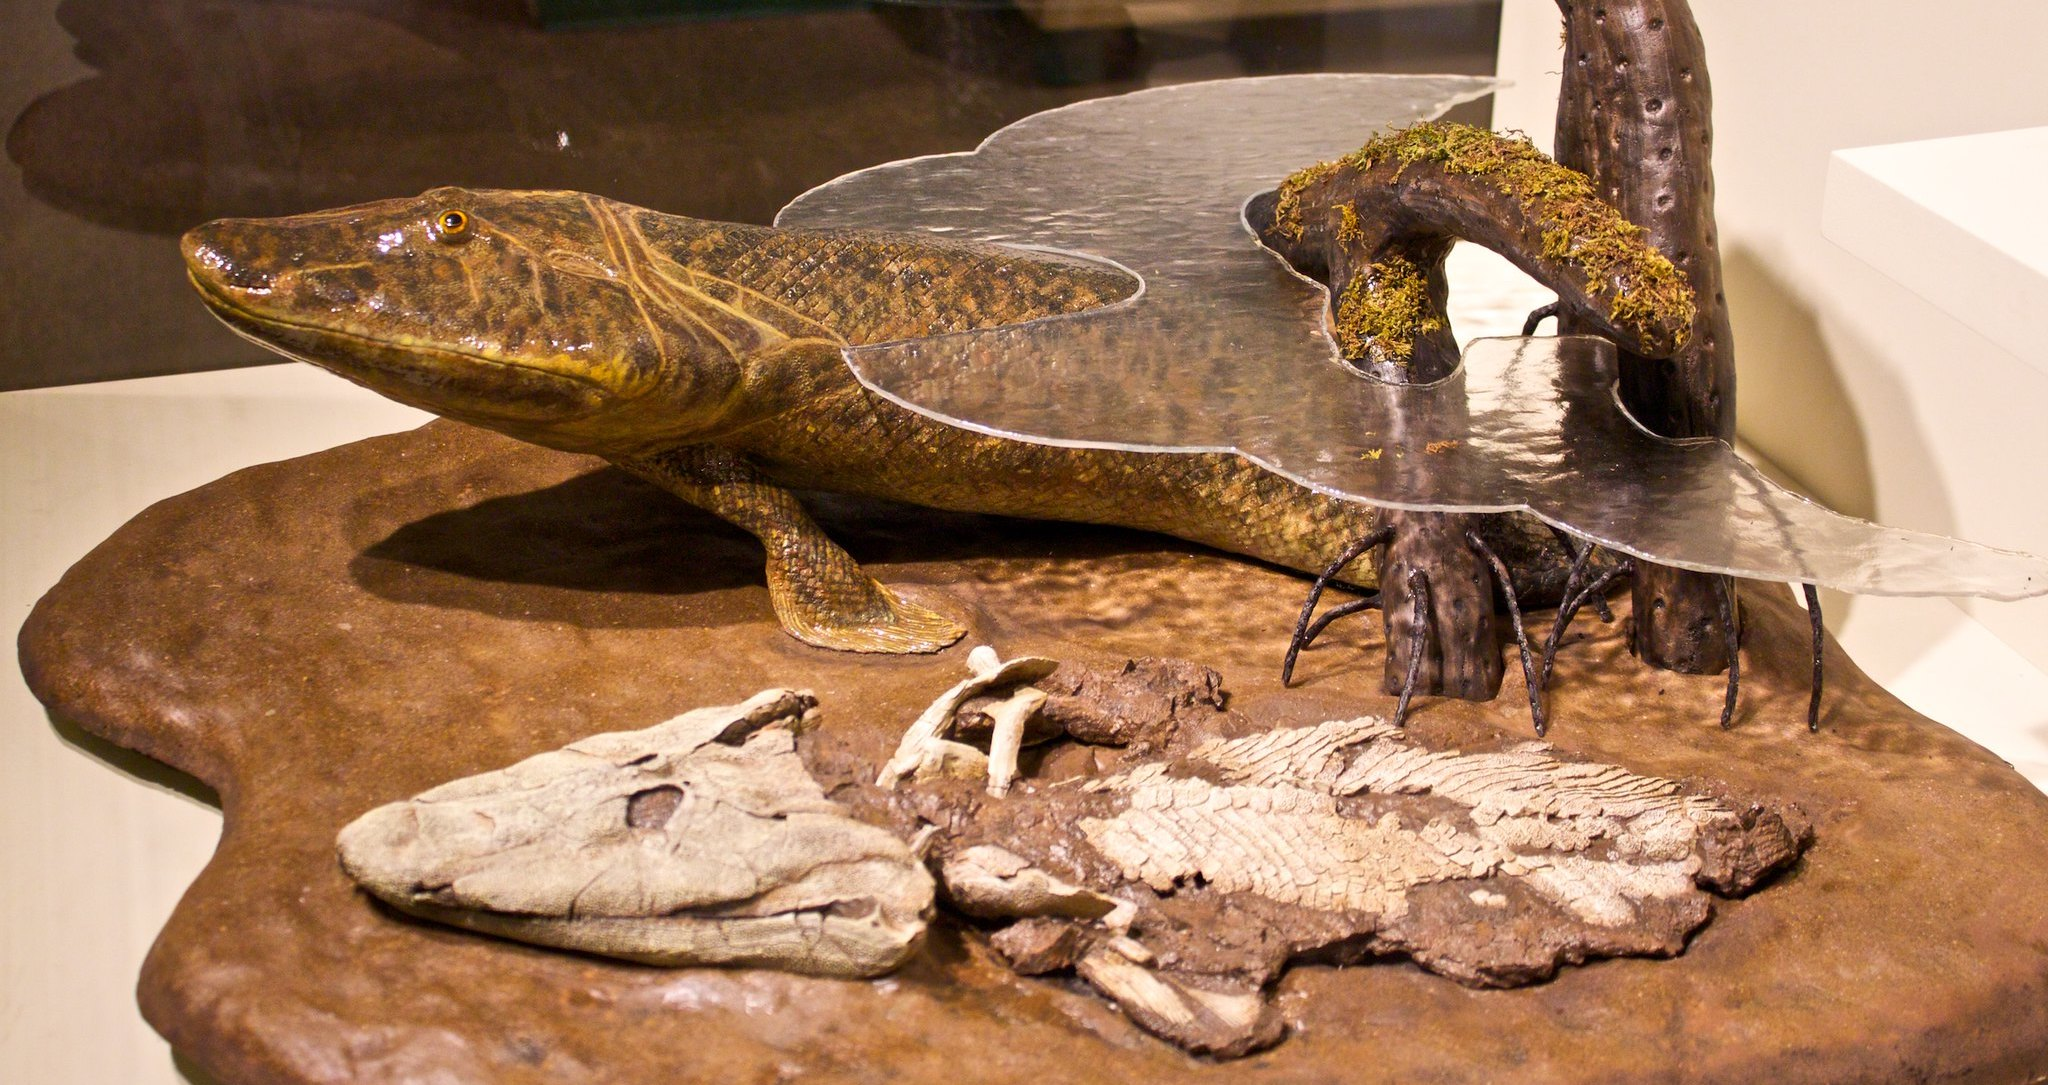
\includegraphics[width=1\linewidth]{images/tiktaalik} \caption{*Tiktaalik roseae*, artist reconstruction and cast of the fossil as displayed at The Harvard Museum of Natural History. Photo by [Maggie](https://www.flickr.com/photos/tankgrrl/4665662106), [CC BY-NC-ND 2.0](https://creativecommons.org/licenses/by-nc-nd/2.0/).}\label{fig:tiktaalik}
\end{figure}

\begin{figure}
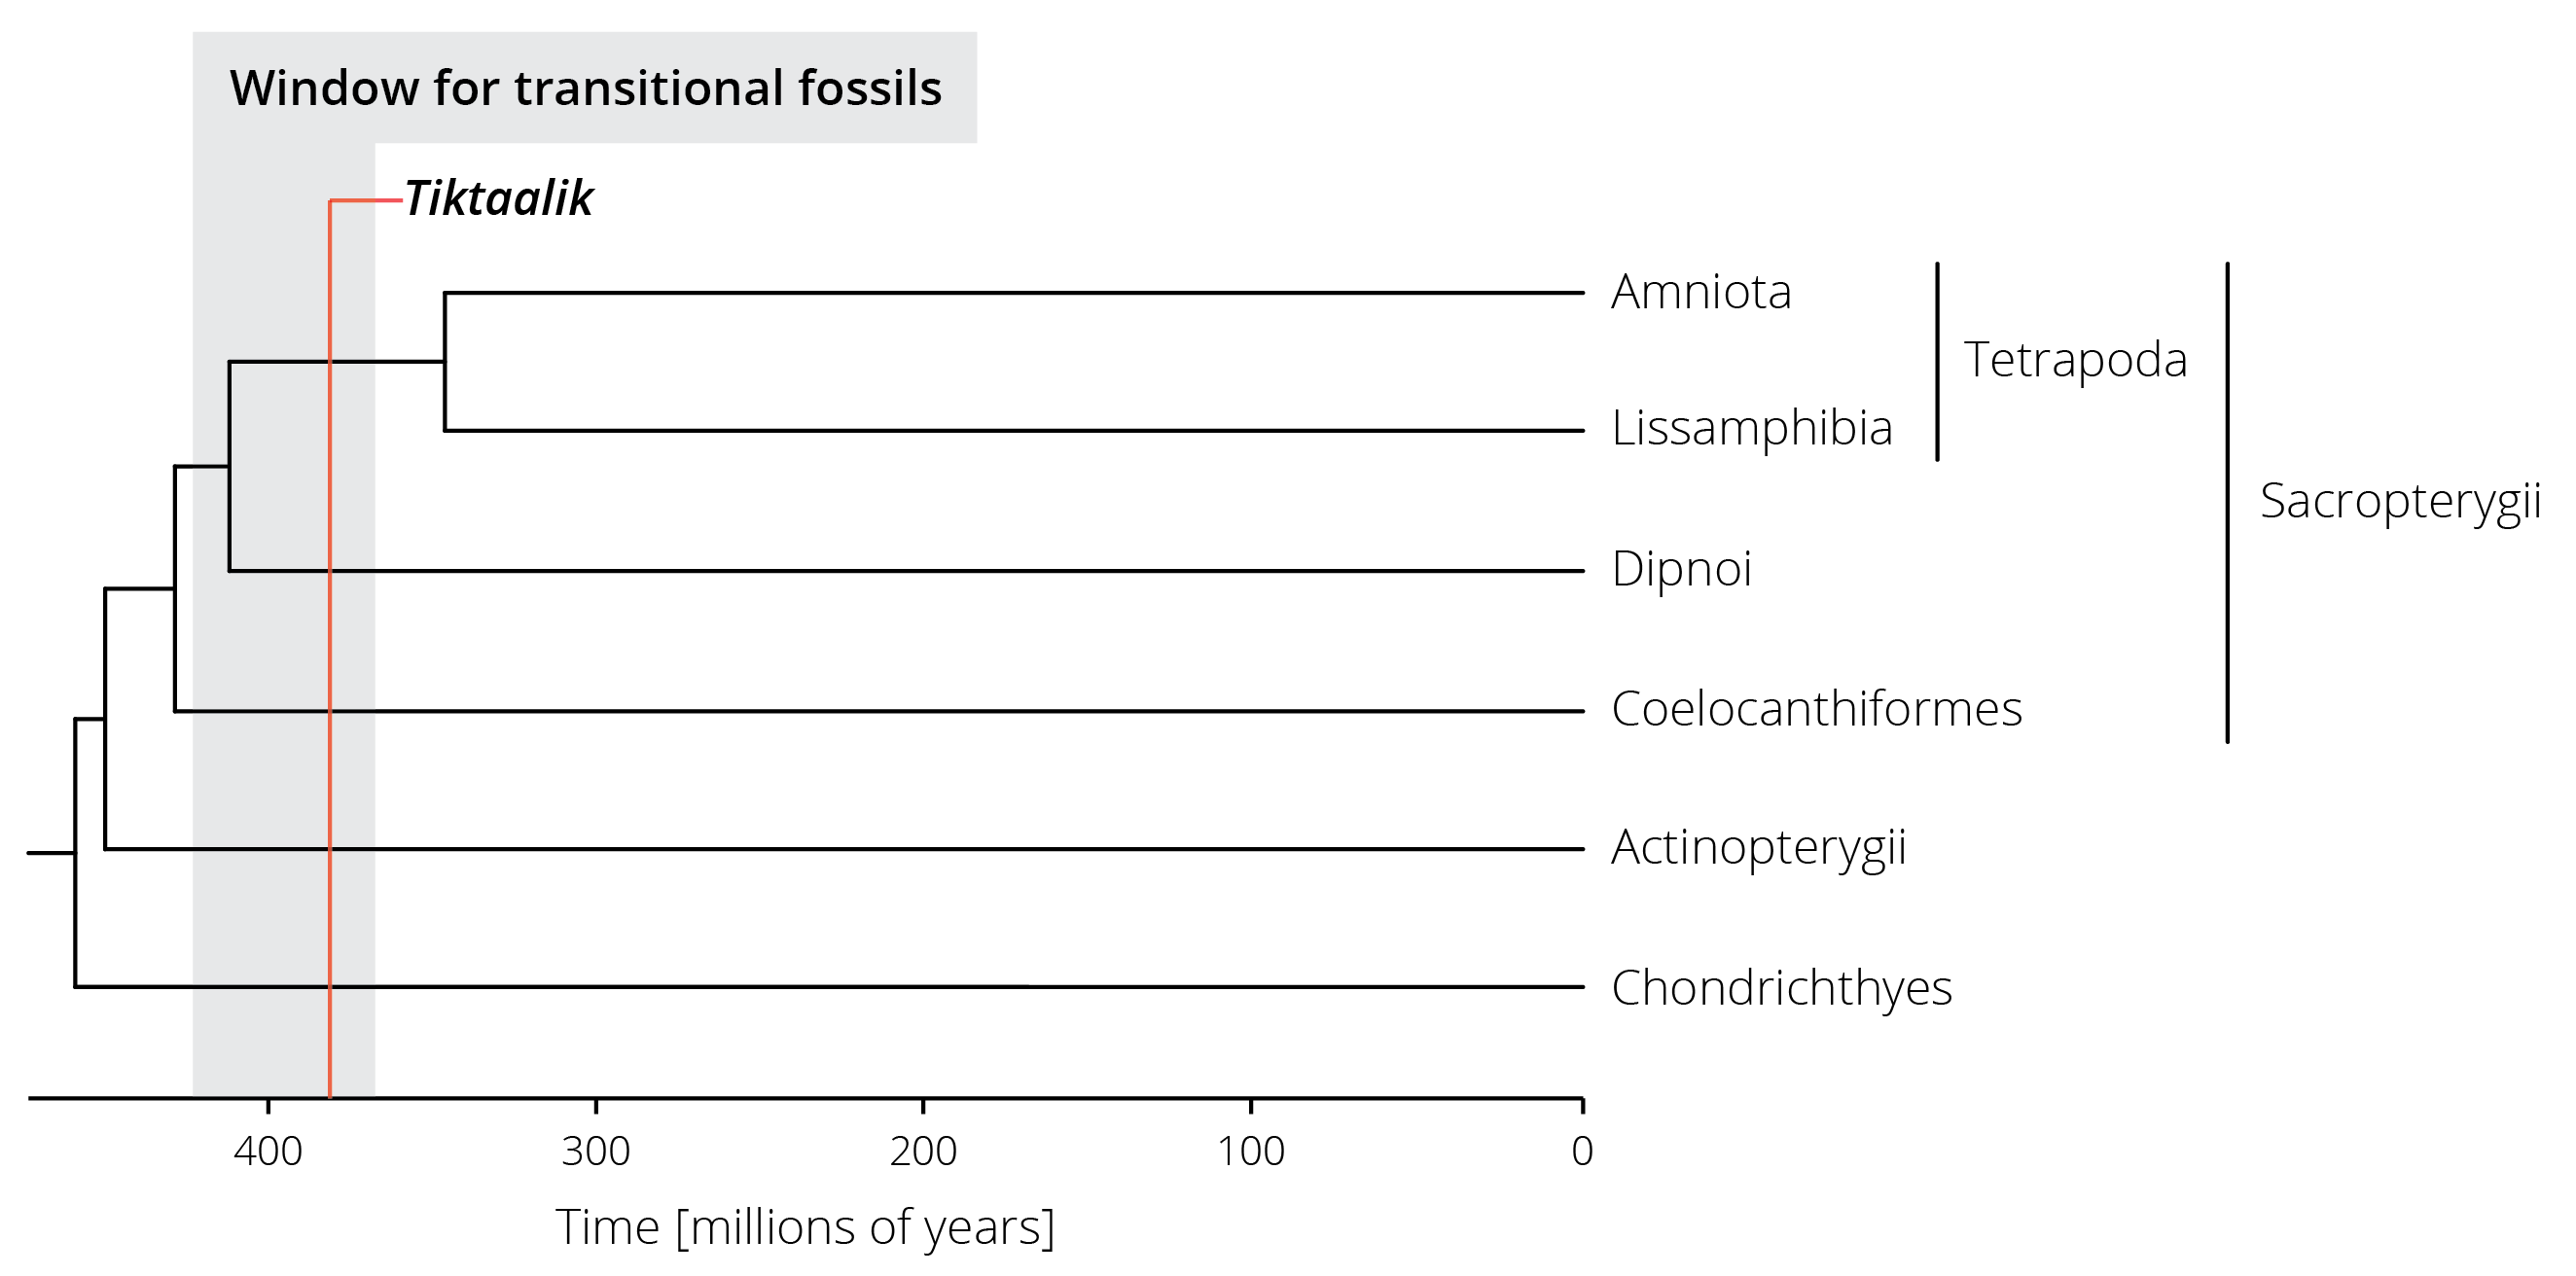
\includegraphics[width=1\linewidth]{images/titaakphyl} \caption{A simplified phylogenetic tree of vertebrates. Terrestrial vertebrates (Tetrapoda) are part of the lobed-finned fishes (Sacropterygii) and split from their sister group (the lungfishes, Dipnoi) between 350 and 425 million years ago. The estimated range for potential transitional fossils is highlighted in gray, the age of the *Tiktaalik* fossil in red. }\label{fig:vertphylo}
\end{figure}

\hypertarget{absence-of-evidence}{%
\section{Absence of Evidence\ldots{}}\label{absence-of-evidence}}

A frequent argument of critics of evolutionary theory (and science in general) is that we cannot explain everything, and indeed there are some major open questions that remain largely unaddressed: How did life on Earth originate? What were the characteristics of the last universal common ancestor of Archaea, Bacteria, and Eukaryotes? How and why did the eukaryotic cell arise? How did the transitional forms between some major taxonomic groups look like? Why is it that so many species reproduce by having sex?

The fact that we do not know the answers to these questions, and many others like them, does not undermine what we do know about evolution and science. It is precisely why evolutionary biology is an exciting field of research. More importantly, \textbf{absence of evidence is not evidence for absence}. For example, gaps in the fossil record and a lack of transitional forms between some taxonomic groups does not negate what we have learned about evolutionary patterns and processes. Perhaps some of these key fossils have just not been found yet, or they may be completely lost to time (because fossilization is actually a rare process). Ultimately, the probability that evolution is true based on other evidence is high enough that a lack of a specific fossil cannot call it into question. Only novel evidence---for example, new fossils that directly contradict our current understanding---has the potential to reshape evolutionary biology. In other words, the burden of proof about any inaccuracies in our current understanding of evolution lies with the critic and not the untouched gaps in our current understanding. And as scientists, it is our day-to-day business to detect and correct those inaccuracies, rather than defending the \emph{status quo} blindly.

\hypertarget{case-study-darwins-finches}{%
\section{Case Study: Darwin's Finches}\label{case-study-darwins-finches}}

For the \href{exercises/BIOL520-ex1.zip}{first case study}, we will take a closer look at some evidence for microevolution, using one of the most iconic study systems in evolutionary biology, the Darwin's finches on the Galapagos Islands. These are the same finches that helped to inspire Darwin, but much of what we know about these finches comes from two biologists, Rosemary and Peter Grant, who have studied these birds in their natural habitats for many decades.

The Grants' primary study site is Daphne Major. With a size of less than half a square kilometer, it is one of the smallest islands in the Galapagos Archipelago (Figure \ref{fig:daphne}). Daphne Major harbors a significant population of the medium ground finch (\emph{Geospiza fortis}, Figure \ref{fig:fortis}), which was the focus of much of the Grants' research. Over decades, they followed this finch population, not only keeping track of individual birds and their offspring, but meticulously measuring the population's phenotypic traits generation after generation. This resulted in a massive, long-term data set that allows us to ask key questions about microevolutionary change. For this exercise, we will take a look at the beak size data the Grants collected from 1972-1994.

Note that this week's case study also provides a general introduction to RStudio and RNotebooks. The practical skills required to complete the exercise are also explained in the section below.

Explore More

To learn more about Rosemary and Peter Grant, check out the \href{https://www.wired.com/2016/10/legendary-biologists-clocked-evolutions-astonishing-speed/}{portrait that Emily Singer wrote for Wired}. If you are interested in their work on finches, I can recommend the popular science book ``\href{https://www.amazon.com/Beak-Finch-Story-Evolution-Time/dp/067973337X}{\emph{The Beak of the Finch: A Story of Evolution in Our Time}}'' by Jonathan Weiner and ``\href{https://www.amazon.com/How-Why-Species-Multiply-Evolutionary/dp/0691149992}{\emph{How and Why Species Multiply: The Radiation of Darwin's Finches}}'' written by the Grants themselves.

\begin{figure}
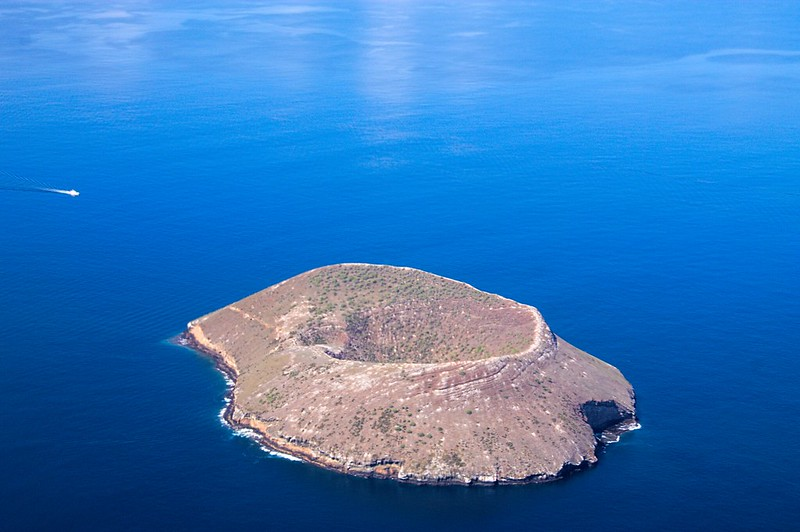
\includegraphics[width=1\linewidth]{images/daphne_major} \caption{Daphne Major, a small rugged island in the Galapagos. Photo by [Sam LaRussa](https://www.flickr.com/photos/blueshift12/16706932513), [CC BY 2.0](https://creativecommons.org/licenses/by/2.0/).}\label{fig:daphne}
\end{figure}

\begin{figure}
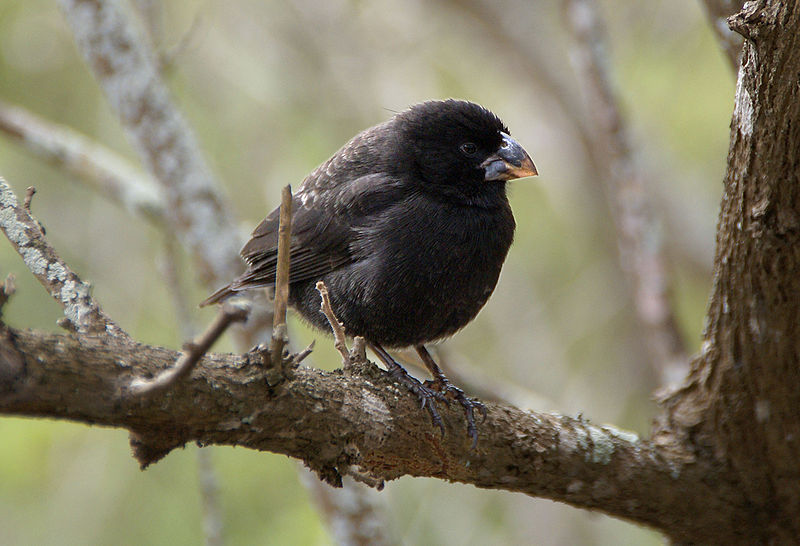
\includegraphics[width=1\linewidth]{images/Geospiza_fortis} \caption{Medium Ground Finch (*Geospiza fortis*), Santa Cruz, Galapagos. Photo by [Putney Mark](http://www.flickr.com/photos/putneymark/1351694843/in/set-72157601810082531/), [CC BY-SA 2.0](https://creativecommons.org/licenses/by-sa/2.0/).}\label{fig:fortis}
\end{figure}

\hypertarget{practical-skills-r-notebooks-and-plotting-with-ggplot}{%
\section{Practical Skills: R Notebooks and Plotting with ggplot}\label{practical-skills-r-notebooks-and-plotting-with-ggplot}}

\hypertarget{r-notebooks}{%
\subsection{R Notebooks}\label{r-notebooks}}

In the \href{what-evolution-is.html\#r}{last chapter}, you learned how to enter commands in the RStudio console to receive an output from R. This showed you the general principle of how you can prompt R to execute any function you want. In reality, you will rarely work in the console, at least for this class. This is because RStudio provides the ability to create \emph{R Notebooks} (*.Rmd files) that allow you to combine text elements (formatted using the Markdown text formatting system) with chunks of code and the code output. Essentially, your R Notebook will contain multiple mini-consoles (the code chunks) with code that you can execute, and the output will be displayed immediately below. The big advantage is that you can create documents that contain computer codes, their outputs (like graphs), and explanatory text (e.g., instructions provided to you or interpretations of the results provided by you).

Each chapter comes with a downloadable *.zip file that contains a folder with the materials for the accompanying exercises (see \href{r-exercises.html}{Appendix B} or links on Canvas). Once unzipped, the folder contains a pre-formatted *.Rmd file as well as additional files, like data sets and images. To avoid issues with the import of data and the display of images, it is important to you keep all files together in the same folder as you received them. If you want to move the files (for example from your \emph{Downloads} folder to your \emph{Class} folder), I recommend that you move the entire folder containing the exercise files (rather than the individual files).

Once you downloaded the files associated with the first exercise, you can open the *.Rmd file by double-clicking, and it will automatically open in RStudio. As you can see, there are three main parts to an R Notebook file.

\hypertarget{the-header}{%
\subsubsection*{The Header}\label{the-header}}
\addcontentsline{toc}{subsubsection}{The Header}

The header, which you can see at the beginning of the document, is delineated with three dashes (\texttt{-\/-\/-}) at the beginning and the end. It includes some code that is important for the formatting of output files. This section of the document is pre-formatted, and I would recommend not altering it; there is no reason for you to change the header for any exercises in this course. However, if you would like to learn more about the different header options for your use of R Notebooks in the future, you can find a good tutorial \href{https://bookdown.org/yihui/rmarkdown/html-document.html\#table-of-contents}{here}.

\hypertarget{code-chunks}{%
\subsubsection*{Code Chunks}\label{code-chunks}}
\addcontentsline{toc}{subsubsection}{Code Chunks}

Code chunks are delineated with three ticks (\texttt{\textquotesingle{}\textquotesingle{}\textquotesingle{}}) at the beginning and the end, and the \texttt{\{r\}} after the first set of ticks lets your computer know that you will be using the R programming language. You can always add a code chunk by clicking ``Insert \textgreater{} Code Chunk \textgreater{} R'' in the RStudio menu, although we usually already created all the chunks that you will need. Any text within a chunk, if written correctly, represents executable code, which R can interpret as a command to execute certain tasks. You can make your computer execute the code in a chunk by pressing the small, green play arrow in the top right corner of each chunk, or you can just highlight the code and press command+enter (control+enter on PC). When you execute the code, the output will automatically appear below the code chunk.

Sometimes you will find us using hash tags (\texttt{\#}) within code chunks. Hash tags ``silence'' the code that follows on the same line, such that the computer jumps over that section when executing the code. That is useful for code annotation, and you will frequently see us using the hash tags to add instructions or explanations.

\hypertarget{text}{%
\subsubsection*{Text}\label{text}}
\addcontentsline{toc}{subsubsection}{Text}

The text in between code chunks is just that: text. We will use these sections to provide you with background information and discussion prompts, and you will use these sections to respond to questions and offer your interpretations of data. Sections where you need to write something are always highlighted in \emph{italics} (designated with asterisks in the source code). You can use a variety of Markdown prompts to format your text (see \href{https://rstudio.com/wp-content/uploads/2015/02/rmarkdown-cheatsheet.pdf}{here} for a cheat sheet), although the current version of RStudio allows you to change formatting with a click of a button, just like other word processing software.

\hypertarget{html-preview-and-output}{%
\subsubsection*{HTML Preview and Output}\label{html-preview-and-output}}
\addcontentsline{toc}{subsubsection}{HTML Preview and Output}

A key strength of the R Notebook system is that you can output your notebook in a wide variety of file formats that automatically integrate text, code, and code output. In fact, this book has entirely been written in RStudio!

To generate an output, your R Notebook (including text, code chunks, and the outputs from your code) can be automatically ``knitted'' into an HTML file. You can click ``Preview \textgreater{} Preview Notebook'' (or ``Knit \textgreater{} Knit to HTML'') to see the live HTML file as you are working on your R Notebook (just make sure to save to update), and you can find the shareable *.html file in the same folder as your *.Rmd-file. The *.html file will have the same file name as your *.Rmd file with ``.nb'' added to it.

\hypertarget{libraries}{%
\subsection{Using Libraries}\label{libraries}}

When you install R, your computer can understand and execute a number of commands. This is what is known as ``Base R''. The power of R, however, is that you can expand the number of commands your computer can understand by installing and loading additional R packages (also called libraries). There are R packages specialized for pretty much any area of biology, providing a capability to analyze data from the level of genes and genomes to ecosystem level processes. We will frequently use a package called \texttt{ggplot2}, which allows for plotting data.

\hypertarget{installing-libraries}{%
\subsubsection*{Installing Libraries}\label{installing-libraries}}
\addcontentsline{toc}{subsubsection}{Installing Libraries}

To successfully complete some of the R exercises, you will need to install additional libraries. To download and install new R packages, go to ``Tools \textgreater{} Install Packages\ldots{}'' and type in the name of the package you want to install (\emph{e.g.}, ``ggplot2''). Alternatively, you can use the \texttt{install.packages()} command as in the following code chunk:

\begin{Shaded}
\begin{Highlighting}[]
\CommentTok{\#To install ggplot2, execute the following code:}
\NormalTok{install}\AttributeTok{.packages}\NormalTok{(}\StringTok{"ggplot2"}\NormalTok{)}
\end{Highlighting}
\end{Shaded}


\includegraphics[width=0.20833in,height=\textheight]{images/important.png} \textbf{Important Note 1}

You only need to install packages once unless you re-install R. I recommend deleting code chunks with \texttt{install.packages()} prompts after you run them successfully, or you can silence them by adding a hash tag in front of the particular line of code. Failure to deactivate package installation code can lead to errors during the knitting of HTML outputs.


\includegraphics[width=0.20833in,height=\textheight]{images/important.png} \textbf{Important Note 2}

Two common problems might occur when you are installing R packages. If it looks like you're installation process is just not making any progress, you might have to respond to queries in the Console:

\begin{enumerate}
\def\labelenumi{\arabic{enumi}.}
\item
  Some installations require updates of packages that are already present. In that case, you will see a prompt in the Console that looks something like this: \texttt{Update\ all/some/none?\ {[}a/s/n{]}:} Just enter ``a'' and press enter.
\item
  Another common prompt is \texttt{Do\ you\ want\ to\ install\ from\ sources\ the\ package\ which\ needs\ compilation?\ {[}yes/no/cancel{]}:} In this case, enter ``y'' and press enter.
\end{enumerate}

\hypertarget{loading-libraries}{%
\subsubsection*{Loading Libraries}\label{loading-libraries}}
\addcontentsline{toc}{subsubsection}{Loading Libraries}

To make use of installed libraries, you also need to load the libraries \emph{every time} you use R (\emph{i.e.}, every time you restart the program). You can do this with the \texttt{library()} command, and you will find a code chunk prompting you to load all required libraries at the beginning of each R Notebook. For example, the following code chunk loads the \texttt{ggplot2} library:

\begin{Shaded}
\begin{Highlighting}[]
\CommentTok{\#Note that loading a library does not lead to an output}
\FunctionTok{library}\NormalTok{(ggplot2)}
\end{Highlighting}
\end{Shaded}


\includegraphics[width=0.20833in,height=\textheight]{images/important.png} \textbf{Important Note}

You have to re-load your libraries every time you restart RStudio. The most common error students in this class encounter is that a particular function cannot be found:

\begin{verbatim}
 Error in function.x(): could not find function "function.x"
\end{verbatim}

This means that the function name is either misspelled, or the library containing a particular function has not been loaded (so R does not actually understand the command you are entering).

\hypertarget{import-data}{%
\subsection{Importing Data}\label{import-data}}

For most R exercises, you will work with real data sets that illuminate evolutionary concepts. Data sets will typically be provided as *.csv files (which stands for comma-separated values). *.csv files are essentially text files containing data tables, and you can also open these in any text editor or Excel. If you do so, you will see a data structure familiar from regular spreadsheets: different variables are organized in columns, and observations are organized in rows.

\hypertarget{setting-your-working-directory}{%
\subsubsection*{Setting Your Working Directory}\label{setting-your-working-directory}}
\addcontentsline{toc}{subsubsection}{Setting Your Working Directory}

Having a well-organized file structure is critical to avoid issues with coding, because you will frequently read in data files, and you need to make sure that R knows where to look for those files. Unless otherwise specified, R will only look for files you may want to import in a particular folder called the working directory. If you are not sure what your current working directory is, you can simply execute the command \texttt{getwd()} in the console, and R will tell your the current working directory.

If you move the exercise files around (or if you are working on your own projects), you need to make sure that R is looking for the files in the right folder. To do so, you need to set the working directory with the \texttt{setwd()} command using the path to your specific folder.

\begin{Shaded}
\begin{Highlighting}[]
\NormalTok{setwd(}\StringTok{"Path"}\NormalTok{)}
\end{Highlighting}
\end{Shaded}

Note that the path on a Mac usually looks something like this: \texttt{/Users/michitobler/Documents}

On a Windows PC, it looks something like this: \texttt{C:\textbackslash{}Users\textbackslash{}michitobler\textbackslash{}Documents}


\includegraphics[width=0.20833in,height=\textheight]{images/important.png} \textbf{Important Note}

If you don't want to deal with having to set your working directory, simply follow the advice from above: Retain your *.Rmd file and all the additional files together in the same folder. If you open the *.Rmd file by double-clicking, the working directory should be set automatically, and R will look in the right spot for files you may want to import.

\hypertarget{reading-a-.csv-file}{%
\subsubsection*{Reading a *.csv File}\label{reading-a-.csv-file}}
\addcontentsline{toc}{subsubsection}{Reading a *.csv File}

To import data in the form of *.csv files, you can use R's \texttt{read.csv()} function. In the code chunk below, you can import a simple test data set (\href{data/test_data.csv}{test\_data.csv}) provided with this chapter that includes three variables: sex, length, and mass of individuals in a population.

\begin{Shaded}
\begin{Highlighting}[]
\CommentTok{\#The line of code simply prompts the computer to read the "test\_data.csv" file and generate a data.frame called test.data}
\CommentTok{\#Note that the file encoding flag simply indicates that the file was generated on a Mac (the operating system I use). It helps to prevent issues for Windows users.}
\NormalTok{test.data }\OtherTok{\textless{}{-}} \FunctionTok{read.csv}\NormalTok{(}\StringTok{"data/test\_data.csv"}\NormalTok{, }\AttributeTok{fileEncoding =} \StringTok{\textquotesingle{}UTF{-}8{-}BOM\textquotesingle{}}\NormalTok{)}
\end{Highlighting}
\end{Shaded}

If this worked correctly, you should now see a new data frame called \texttt{test.data} in your work space (Global Environment; top right panel). You can double click it to view it or execute \texttt{View(test.data)} in the console as described on \href{what-evolution-is.html\#data-frame}{Chapter 1}. There should be three columns: sex, length, and mass.

\hypertarget{graphing-data}{%
\subsection{Graphing Data}\label{graphing-data}}

A key learning objective of this course is that you learn to visualize and interpret data to address different evolutionary hypotheses. In the following sections, I will explain step by step (that is code line by code line) how to make a simple graph with our test data. Let's aim to make a scatter plot showing the relationship between length and mass of individuals in the population. The process is not much different than sketching a graph by hand and layering different parts of the graph on top of each other, just that you use words (code) to make the computer draw. To graph data, we will primarily use the \texttt{ggplot()} function that comes with the \texttt{ggplot2} library.

\hypertarget{defining-the-axes-and-coordinate-system}{%
\subsubsection*{Defining the Axes and Coordinate System}\label{defining-the-axes-and-coordinate-system}}
\addcontentsline{toc}{subsubsection}{Defining the Axes and Coordinate System}

The first step of making any graph is to define the axes and establish the coordinate grid that allows for the plotting of the data. To do this, R first needs to know what data frame the data is stored in (in our case, the data frame is called \texttt{test.data}). The axes are then defined by specifying the aesthetics \texttt{aes()} within the \texttt{ggplot} function, as shown below.

\begin{Shaded}
\begin{Highlighting}[]
\CommentTok{\#This line of code calls for the ggplot function (a plotting function) and makes a grid based on the test.data data frame, using length as the x axis and mass as the y axis}
\FunctionTok{ggplot}\NormalTok{(test.data, }\FunctionTok{aes}\NormalTok{(}\AttributeTok{x=}\NormalTok{length, }\AttributeTok{y=}\NormalTok{mass))}
\end{Highlighting}
\end{Shaded}

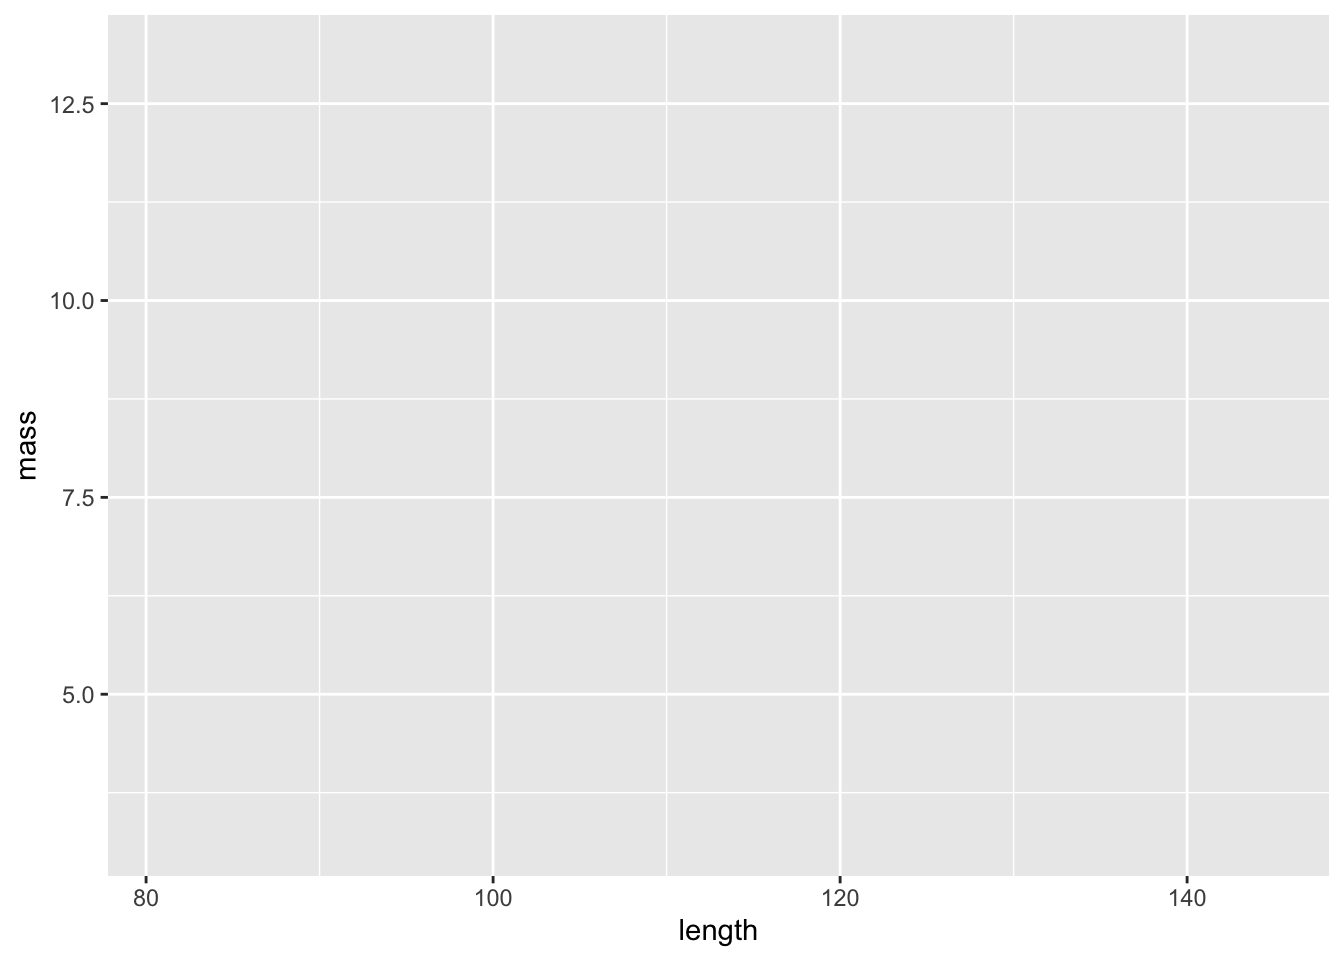
\includegraphics{Primer2Evolution_files/figure-latex/coord-1.pdf}

The output is a simple coordinate system based on the data we provided, with length as the x-axis and mass as the y-axis.

\hypertarget{adding-a-layer-with-data-points}{%
\subsubsection*{Adding a Layer with Data Points}\label{adding-a-layer-with-data-points}}
\addcontentsline{toc}{subsubsection}{Adding a Layer with Data Points}

The second step is to draw the actual data into the established coordinate system. To do so, you just need to tell the program what kind of graph you want to draw. Different graph types in ggplot are referred to as geoms (geometries), and a scatter plot is designated as \texttt{geom\_point()}. You can add that to your existing code describing the coordinate system with a plus sign.

\begin{Shaded}
\begin{Highlighting}[]
\FunctionTok{ggplot}\NormalTok{(test.data, }\FunctionTok{aes}\NormalTok{(}\AttributeTok{x=}\NormalTok{length, }\AttributeTok{y=}\NormalTok{mass)) }\SpecialCharTok{+}
  \FunctionTok{geom\_point}\NormalTok{()}
\end{Highlighting}
\end{Shaded}

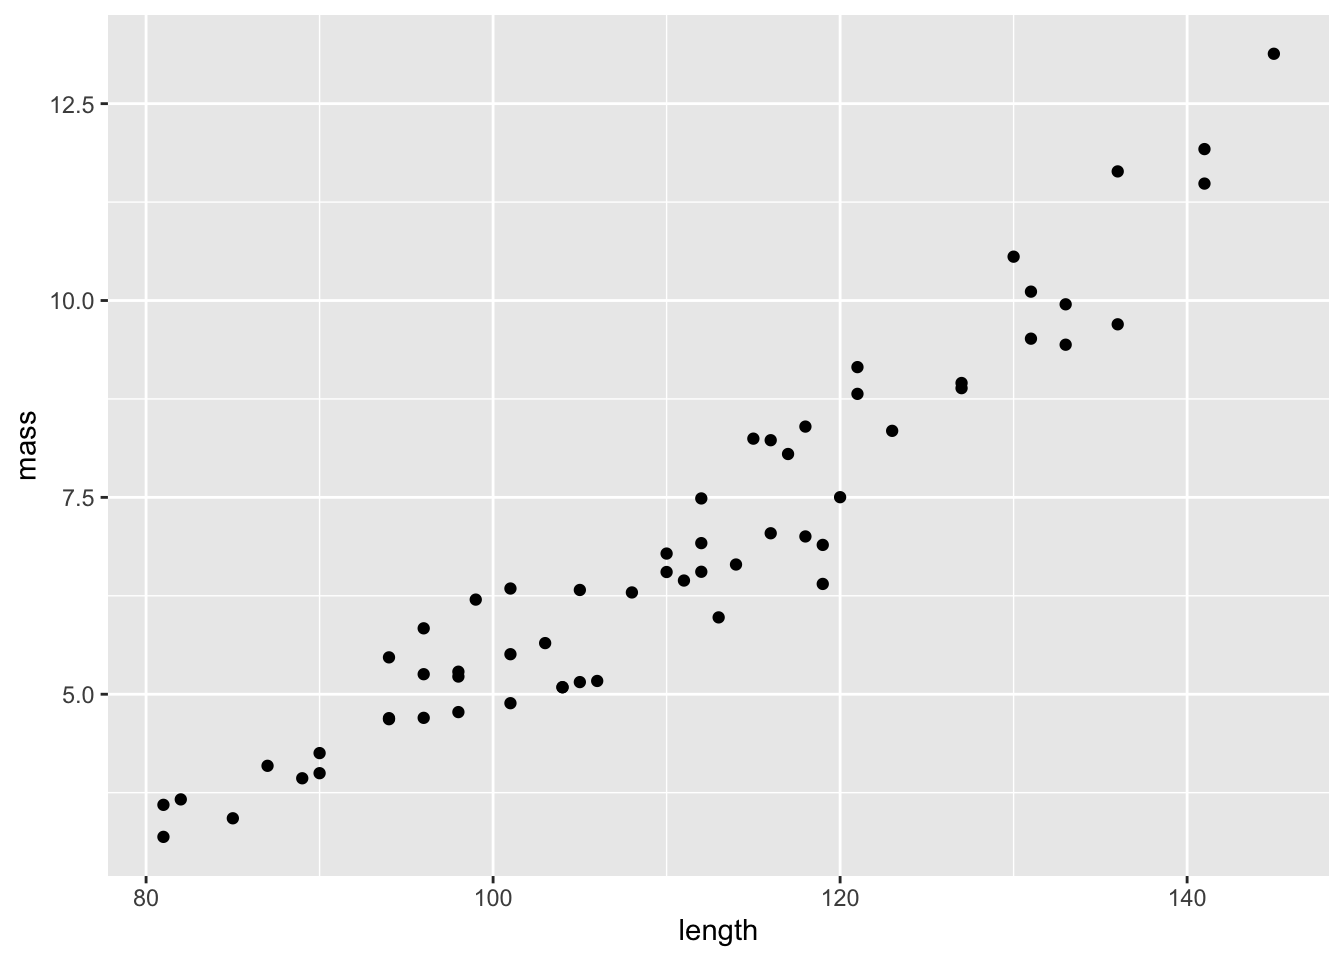
\includegraphics{Primer2Evolution_files/figure-latex/points-1.pdf}

For an overview of some of the graph types (geoms) ggplot offers, check \href{https://www.r-graph-gallery.com/}{here}. In the coming chapters, I will introduce you to a variety of geoms that you can use to visualize different types of data.

\hypertarget{adding-a-trendline}{%
\subsubsection*{Adding a Trendline}\label{adding-a-trendline}}
\addcontentsline{toc}{subsubsection}{Adding a Trendline}

Whenever we look at the relationship between two variables, we may want to add a trendline. You can add a trendline by adding the \texttt{geom\_smooth()} function to your existing code. \texttt{method="lm"} within the \texttt{geom\_smooth()} function indicates that we want to draw a straight line (linear model, \texttt{lm}). \texttt{se=FALSE} indicates that we do not want to draw a confidence interval around the estimated best-fit line. Change it to \texttt{se=TRUE} and see what happens.

\begin{Shaded}
\begin{Highlighting}[]
\CommentTok{\#The code within the brackets of the geom\_smooth command specifies some additional options, namely that we want to draw a straight line (method="lm") and that we do not want to show the confidence interval (se=FALSE).}
\FunctionTok{ggplot}\NormalTok{(test.data, }\FunctionTok{aes}\NormalTok{(}\AttributeTok{x=}\NormalTok{length, }\AttributeTok{y=}\NormalTok{mass)) }\SpecialCharTok{+}
  \FunctionTok{geom\_point}\NormalTok{() }\SpecialCharTok{+}
  \FunctionTok{geom\_smooth}\NormalTok{(}\AttributeTok{method=}\StringTok{"lm"}\NormalTok{, }\AttributeTok{se=}\ConstantTok{FALSE}\NormalTok{)}
\end{Highlighting}
\end{Shaded}

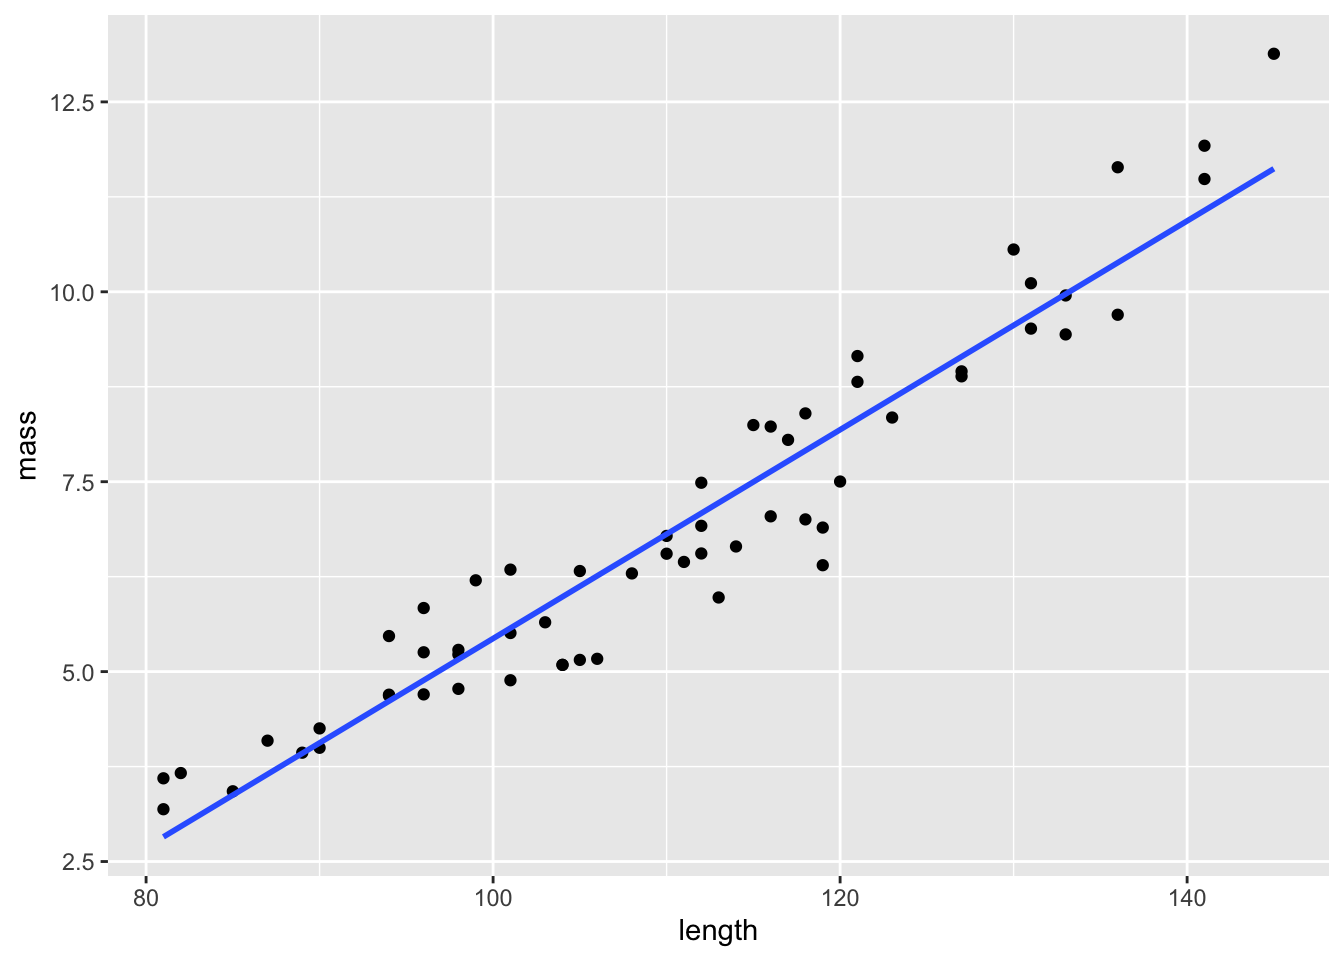
\includegraphics{Primer2Evolution_files/figure-latex/trend-1.pdf}

\hypertarget{changing-the-axes-labels}{%
\subsubsection*{Changing the Axes Labels}\label{changing-the-axes-labels}}
\addcontentsline{toc}{subsubsection}{Changing the Axes Labels}

The variable names in the data frame do not always provide the clearest description of what a variable means. We can modify the x and y axis labels using the \texttt{xlab()} and \texttt{ylab()} commands, respectively. Note that labels need to be written in quotation marks.

\begin{Shaded}
\begin{Highlighting}[]
\CommentTok{\#Simply add the new label text in quotation marks}
\FunctionTok{ggplot}\NormalTok{(test.data, }\FunctionTok{aes}\NormalTok{(}\AttributeTok{x=}\NormalTok{length, }\AttributeTok{y=}\NormalTok{mass)) }\SpecialCharTok{+}
  \FunctionTok{geom\_point}\NormalTok{() }\SpecialCharTok{+}
  \FunctionTok{geom\_smooth}\NormalTok{(}\AttributeTok{method=}\StringTok{"lm"}\NormalTok{, }\AttributeTok{se=}\ConstantTok{FALSE}\NormalTok{) }\SpecialCharTok{+}
  \FunctionTok{xlab}\NormalTok{(}\StringTok{"Body length in cm"}\NormalTok{) }\SpecialCharTok{+}
  \FunctionTok{ylab}\NormalTok{(}\StringTok{"Body mass in kg"}\NormalTok{)}
\end{Highlighting}
\end{Shaded}

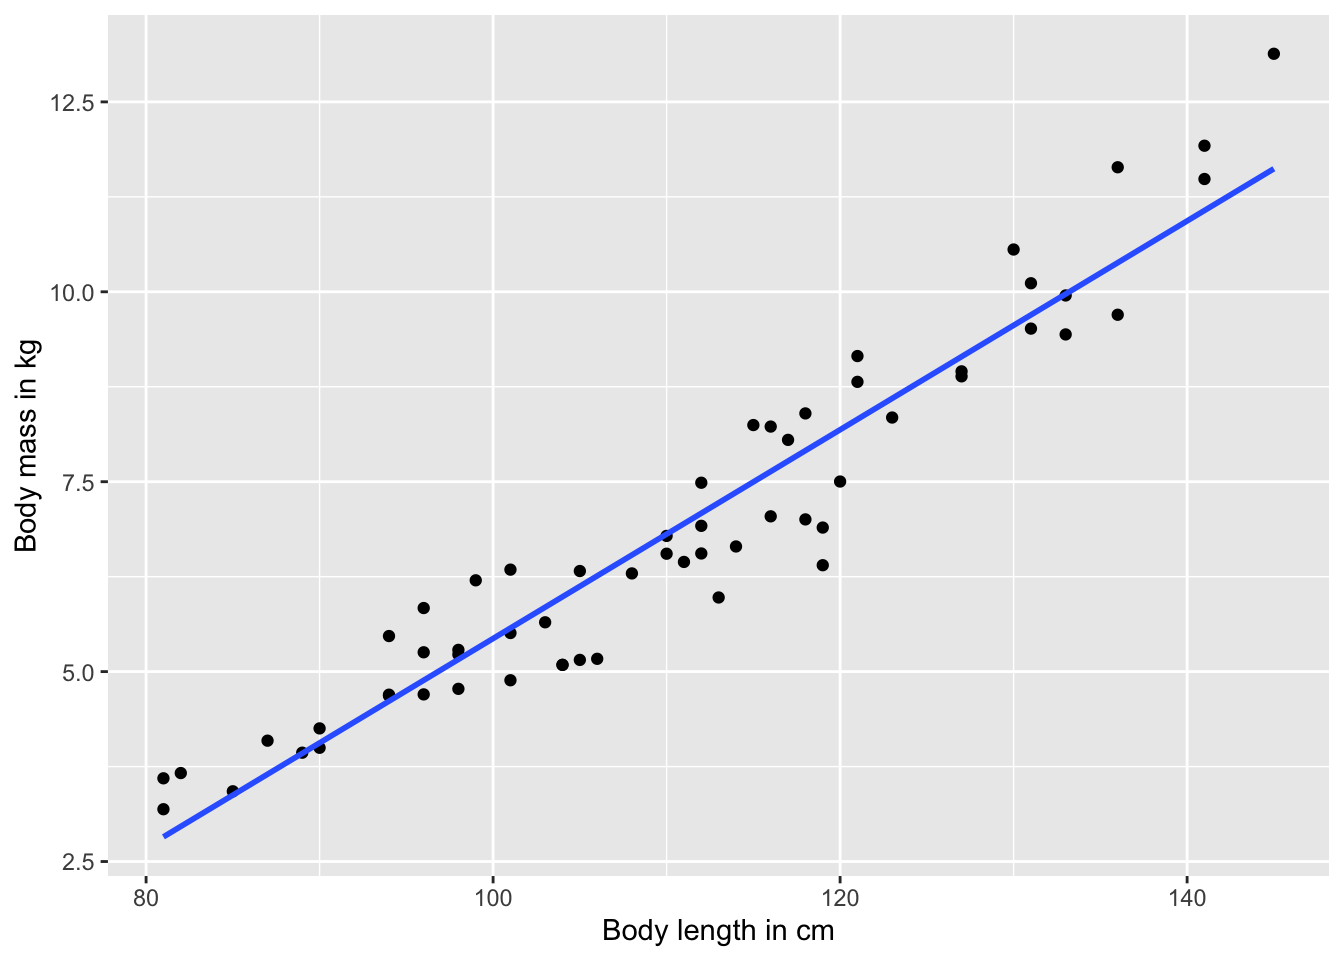
\includegraphics{Primer2Evolution_files/figure-latex/labels-1.pdf}

Note that an alternative way of changing the axes labels is to use the \texttt{labs()} function. Specifically, \texttt{labs(x="Body\ length\ in\ cm",\ y="Body\ mass\ in\ kg")} will provide the same result as the code used above.

\hypertarget{adding-additional-complexity}{%
\subsubsection*{Adding Additional Complexity}\label{adding-additional-complexity}}
\addcontentsline{toc}{subsubsection}{Adding Additional Complexity}

If you look at the data frame, you will see that we do not only have information about the length and mass of individuals in the population, but also their sex. So, we may want to account for potential sex differences in the relationship between length and mass. To do so, we can color-code individual points based on the sex of the individual by adding another term of the aesthetics of the \texttt{ggplot()} function (\texttt{color=sex}):

\begin{Shaded}
\begin{Highlighting}[]
\FunctionTok{ggplot}\NormalTok{(test.data, }\FunctionTok{aes}\NormalTok{(}\AttributeTok{x=}\NormalTok{length, }\AttributeTok{y=}\NormalTok{mass, }\AttributeTok{color=}\NormalTok{sex)) }\SpecialCharTok{+}
  \FunctionTok{geom\_point}\NormalTok{() }\SpecialCharTok{+}
  \FunctionTok{geom\_smooth}\NormalTok{(}\AttributeTok{method=}\StringTok{"lm"}\NormalTok{, }\AttributeTok{se=}\ConstantTok{FALSE}\NormalTok{) }\SpecialCharTok{+}
  \FunctionTok{xlab}\NormalTok{(}\StringTok{"Body length in cm"}\NormalTok{) }\SpecialCharTok{+}
  \FunctionTok{ylab}\NormalTok{(}\StringTok{"Body mass in kg"}\NormalTok{)}
\end{Highlighting}
\end{Shaded}

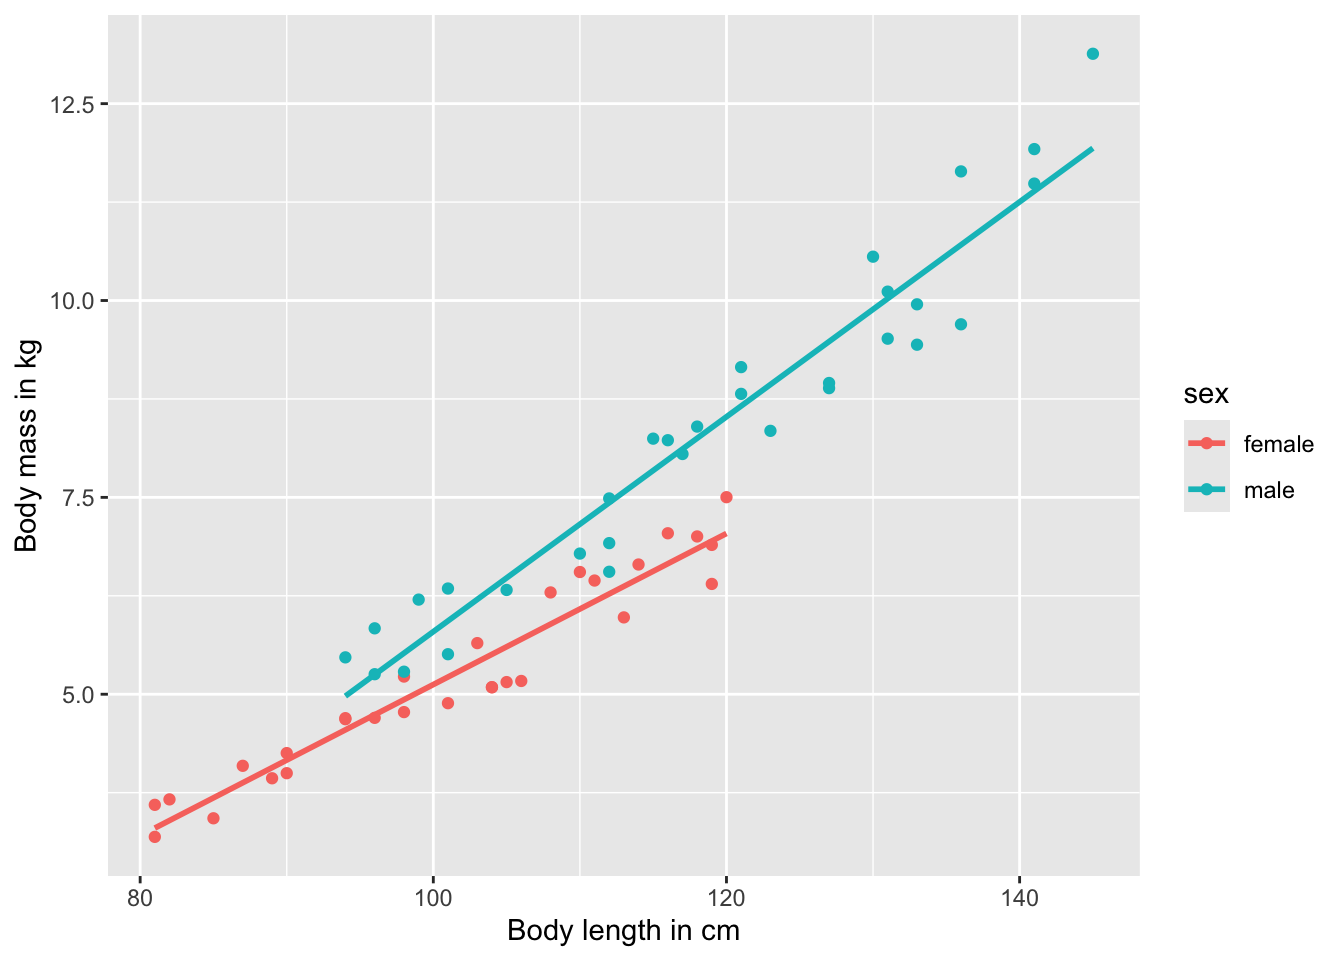
\includegraphics{Primer2Evolution_files/figure-latex/groups-1.pdf}

As you can see, this not only changes the color of individual points, but it also draws a separate regression line for males and females. If you want to change the legend title, you can do this again with the \texttt{labs()} function: \texttt{labs(x="Body\ length\ in\ cm",\ y="Body\ mass\ in\ kg",\ color="Sex")} .

\hypertarget{optional-changing-the-theme}{%
\subsubsection*{Optional: Changing the Theme}\label{optional-changing-the-theme}}
\addcontentsline{toc}{subsubsection}{Optional: Changing the Theme}

I honestly just hate the default theme of \texttt{ggplot()} with its gray background. But you can quickly alter the look of a graph by switching to a number of other possible themes. I personally like the \texttt{theme\_classic()}, but you can customize the look of your graph with any theme you may like (see \href{https://www.datanovia.com/en/blog/ggplot-themes-gallery/\#basic-ggplot}{here}).

\begin{Shaded}
\begin{Highlighting}[]
\FunctionTok{ggplot}\NormalTok{(test.data, }\FunctionTok{aes}\NormalTok{(}\AttributeTok{x=}\NormalTok{length, }\AttributeTok{y=}\NormalTok{mass, }\AttributeTok{color=}\NormalTok{sex)) }\SpecialCharTok{+}
  \FunctionTok{geom\_point}\NormalTok{() }\SpecialCharTok{+}
  \FunctionTok{geom\_smooth}\NormalTok{(}\AttributeTok{method=}\StringTok{"lm"}\NormalTok{, }\AttributeTok{se=}\ConstantTok{FALSE}\NormalTok{) }\SpecialCharTok{+}
  \FunctionTok{xlab}\NormalTok{(}\StringTok{"Body length in cm"}\NormalTok{) }\SpecialCharTok{+}
  \FunctionTok{ylab}\NormalTok{(}\StringTok{"Body mass in kg"}\NormalTok{) }\SpecialCharTok{+}
  \FunctionTok{theme\_classic}\NormalTok{()}
\end{Highlighting}
\end{Shaded}

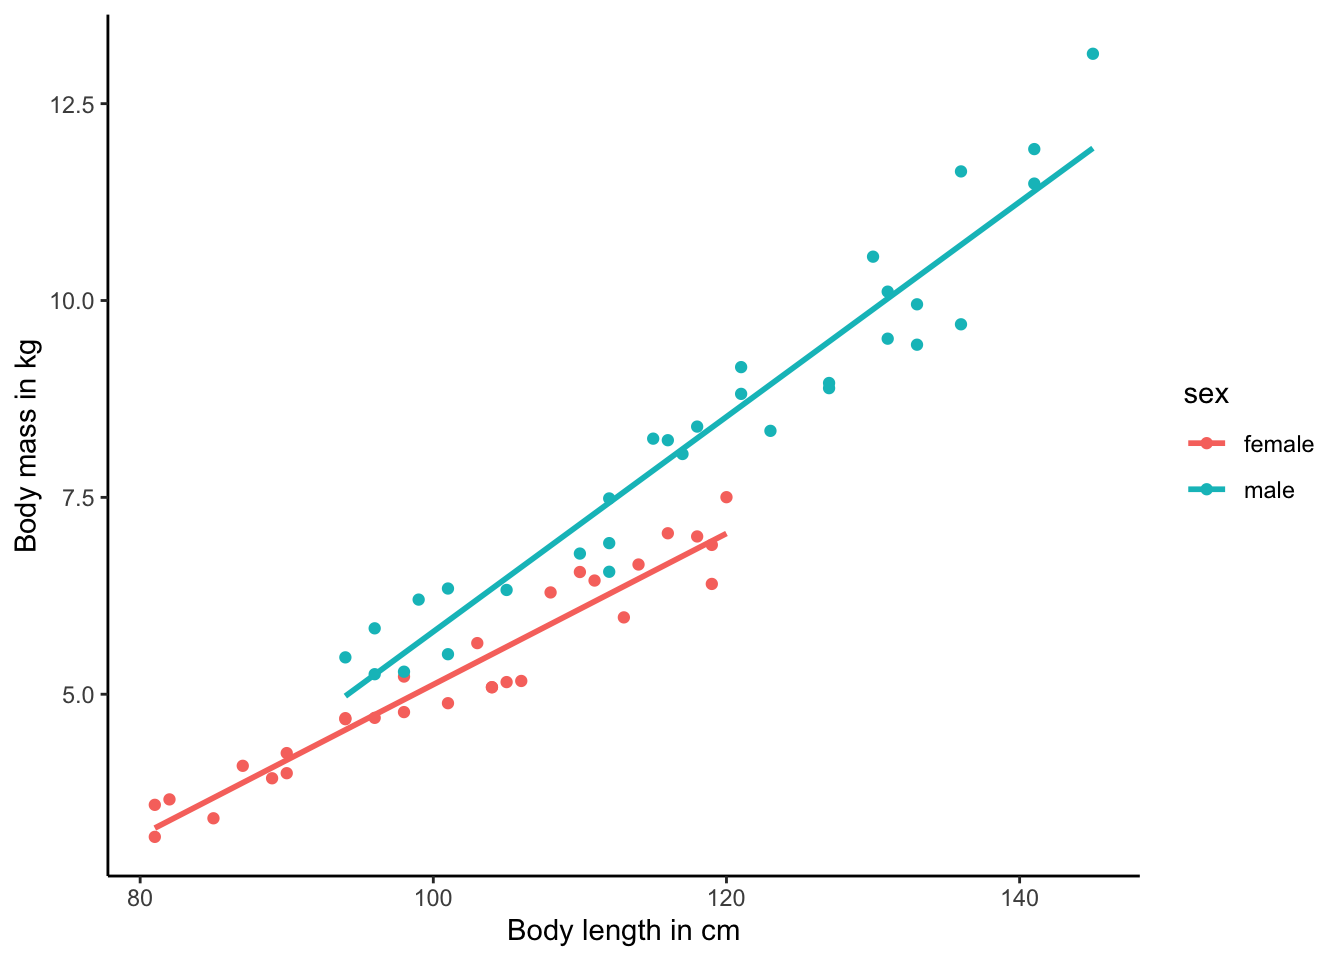
\includegraphics{Primer2Evolution_files/figure-latex/theme-1.pdf}

\hypertarget{optional-changing-to-a-colorblind-friendly-palette}{%
\subsubsection*{Optional: Changing to a Colorblind-Friendly Palette}\label{optional-changing-to-a-colorblind-friendly-palette}}
\addcontentsline{toc}{subsubsection}{Optional: Changing to a Colorblind-Friendly Palette}

ggplot uses a default color palette when you add color to a graph. You may not like that default color scheme, or---if you have impaired color perception---you may find it difficult to distinguish some of the default colors. One simple way of changing the color palette of your graph is to use the \texttt{RColorBrewer} package. If you want to use it, you first need to install that library on your computer, just like you did for \texttt{ggplot2} above:

\begin{Shaded}
\begin{Highlighting}[]
\CommentTok{\#To install RColorBrewer, execute the following code in your Console:}
\NormalTok{install}\AttributeTok{.packages}\NormalTok{(}\StringTok{"RColorBrewer"}\NormalTok{)}
\end{Highlighting}
\end{Shaded}

\texttt{RColorBrewer} includes several color palettes, including options that have been developed for people with color blindness. To see the different colorblind-friendly options, you can simply use the following function:

\begin{Shaded}
\begin{Highlighting}[]
\FunctionTok{display.brewer.all}\NormalTok{(}\AttributeTok{colorblindFriendly =} \ConstantTok{TRUE}\NormalTok{)}
\end{Highlighting}
\end{Shaded}

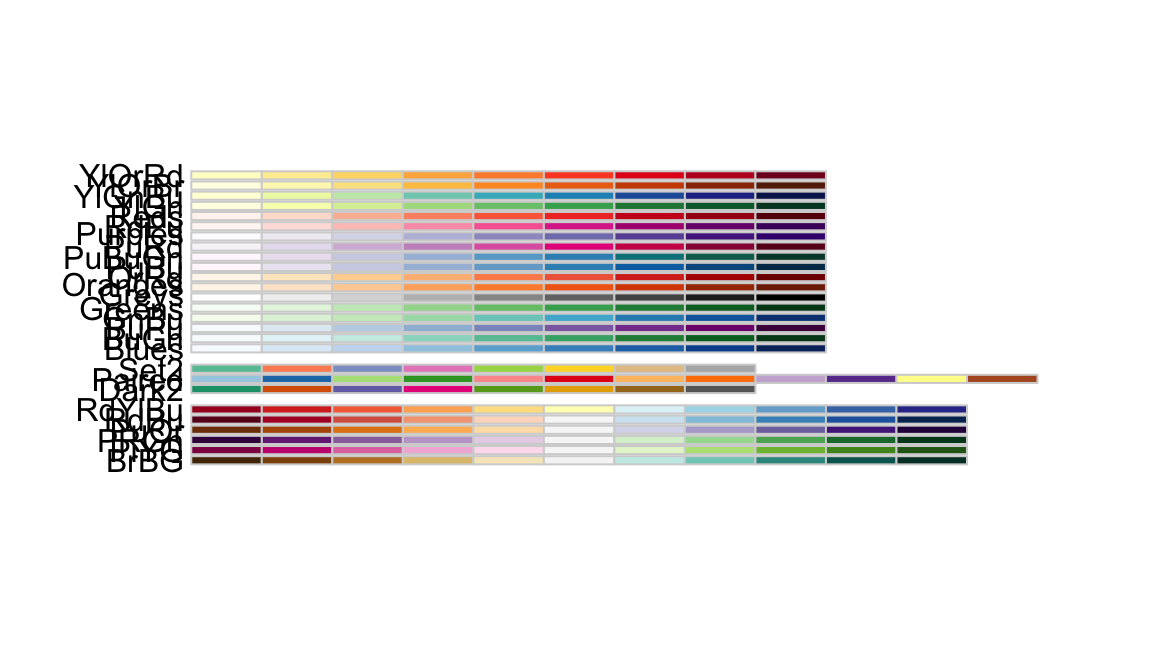
\includegraphics{Primer2Evolution_files/figure-latex/RColBrew-1.pdf}

To change the color scheme of the graph generated with the \texttt{ggplot()}, you can simply use the \texttt{scale\_color\_brewer()} function to designate the desired palette:

\begin{Shaded}
\begin{Highlighting}[]
\FunctionTok{ggplot}\NormalTok{(test.data, }\FunctionTok{aes}\NormalTok{(}\AttributeTok{x=}\NormalTok{length, }\AttributeTok{y=}\NormalTok{mass, }\AttributeTok{color=}\NormalTok{sex)) }\SpecialCharTok{+}
  \FunctionTok{geom\_point}\NormalTok{() }\SpecialCharTok{+}
  \FunctionTok{geom\_smooth}\NormalTok{(}\AttributeTok{method=}\StringTok{"lm"}\NormalTok{, }\AttributeTok{se=}\ConstantTok{FALSE}\NormalTok{) }\SpecialCharTok{+}
  \FunctionTok{xlab}\NormalTok{(}\StringTok{"Body length in cm"}\NormalTok{) }\SpecialCharTok{+}
  \FunctionTok{ylab}\NormalTok{(}\StringTok{"Body mass in kg"}\NormalTok{) }\SpecialCharTok{+}
  \FunctionTok{theme\_classic}\NormalTok{()}\SpecialCharTok{+}
  \FunctionTok{scale\_color\_brewer}\NormalTok{(}\AttributeTok{palette=}\StringTok{"Dark2"}\NormalTok{)}
\end{Highlighting}
\end{Shaded}

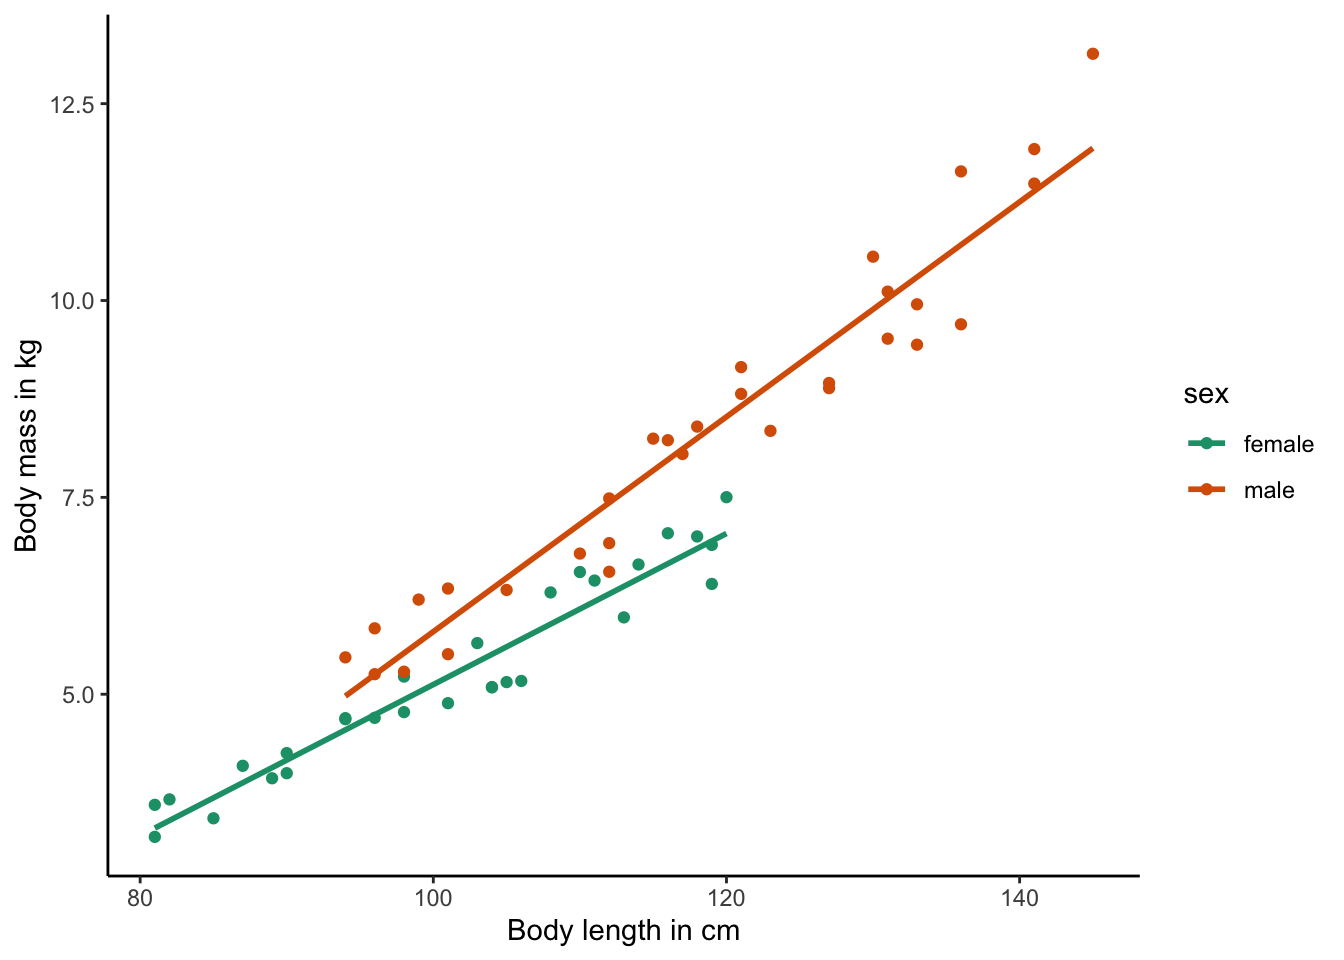
\includegraphics{Primer2Evolution_files/figure-latex/coltheme-1.pdf}

\hypertarget{generating-and-visualizing-aggregate-data}{%
\subsubsection*{Generating and Visualizing Aggregate Data}\label{generating-and-visualizing-aggregate-data}}
\addcontentsline{toc}{subsubsection}{Generating and Visualizing Aggregate Data}

In the exercise associated with this chapter, you will not be plotting data from individuals but rather aggregate data that is compiled from many individuals and provides a mean and a measurement of variation around a mean for different sampling groups. To show you how we can visualize such data as mean (± variation), I am first calculating the mean and standard deviation (sd) of length separate for each sex based on the data above using the \texttt{ddply()} function from the \texttt{plyr} package.

\begin{Shaded}
\begin{Highlighting}[]
\CommentTok{\#Load the plyr package that includes the ddply function}
\FunctionTok{library}\NormalTok{(plyr)}

\CommentTok{\#Use the ddply function to calculate mean and standard deviation of length for each sex}
\NormalTok{sum.stat }\OtherTok{\textless{}{-}} \FunctionTok{ddply}\NormalTok{(test.data,}\SpecialCharTok{\textasciitilde{}}\NormalTok{sex,summarise,}\AttributeTok{mean=}\FunctionTok{mean}\NormalTok{(length),}\AttributeTok{sd=}\FunctionTok{sd}\NormalTok{(length))}
\FunctionTok{print}\NormalTok{(sum.stat)}
\end{Highlighting}
\end{Shaded}

\begin{verbatim}
##      sex     mean       sd
## 1 female 101.2414 12.34520
## 2   male 118.6452 15.05224
\end{verbatim}

To visualize means and standard variations, we can again use the \texttt{ggplot()} function with sex on the x axis and the mean value of length on the y axis (note that we are now referring to the \texttt{sum.stat} data frame that we just created in the last code chunk). As before, we are using \texttt{geom\_point()} to draw our data as points. In addition, we are using \texttt{geom\_errorbar()} to draw the standard deviations around the mean in both directions. You already know all the other code elements from above.

\begin{Shaded}
\begin{Highlighting}[]
\FunctionTok{ggplot}\NormalTok{(sum.stat, }\FunctionTok{aes}\NormalTok{(}\AttributeTok{x=}\NormalTok{sex, }\AttributeTok{y=}\NormalTok{mean)) }\SpecialCharTok{+}
  \FunctionTok{geom\_point}\NormalTok{() }\SpecialCharTok{+}
  \FunctionTok{geom\_errorbar}\NormalTok{(}\FunctionTok{aes}\NormalTok{(}\AttributeTok{ymin=}\NormalTok{mean}\SpecialCharTok{{-}}\NormalTok{sd, }\AttributeTok{ymax=}\NormalTok{mean}\SpecialCharTok{+}\NormalTok{sd), }\AttributeTok{width=}\FloatTok{0.1}\NormalTok{)  }\SpecialCharTok{+}  \CommentTok{\#widfth designates the width of the horizontal bars}
  \FunctionTok{xlab}\NormalTok{(}\StringTok{"Sex"}\NormalTok{) }\SpecialCharTok{+}
  \FunctionTok{ylab}\NormalTok{(}\StringTok{"Mean length [mm]"}\NormalTok{) }\SpecialCharTok{+}
  \FunctionTok{theme\_classic}\NormalTok{()}
\end{Highlighting}
\end{Shaded}

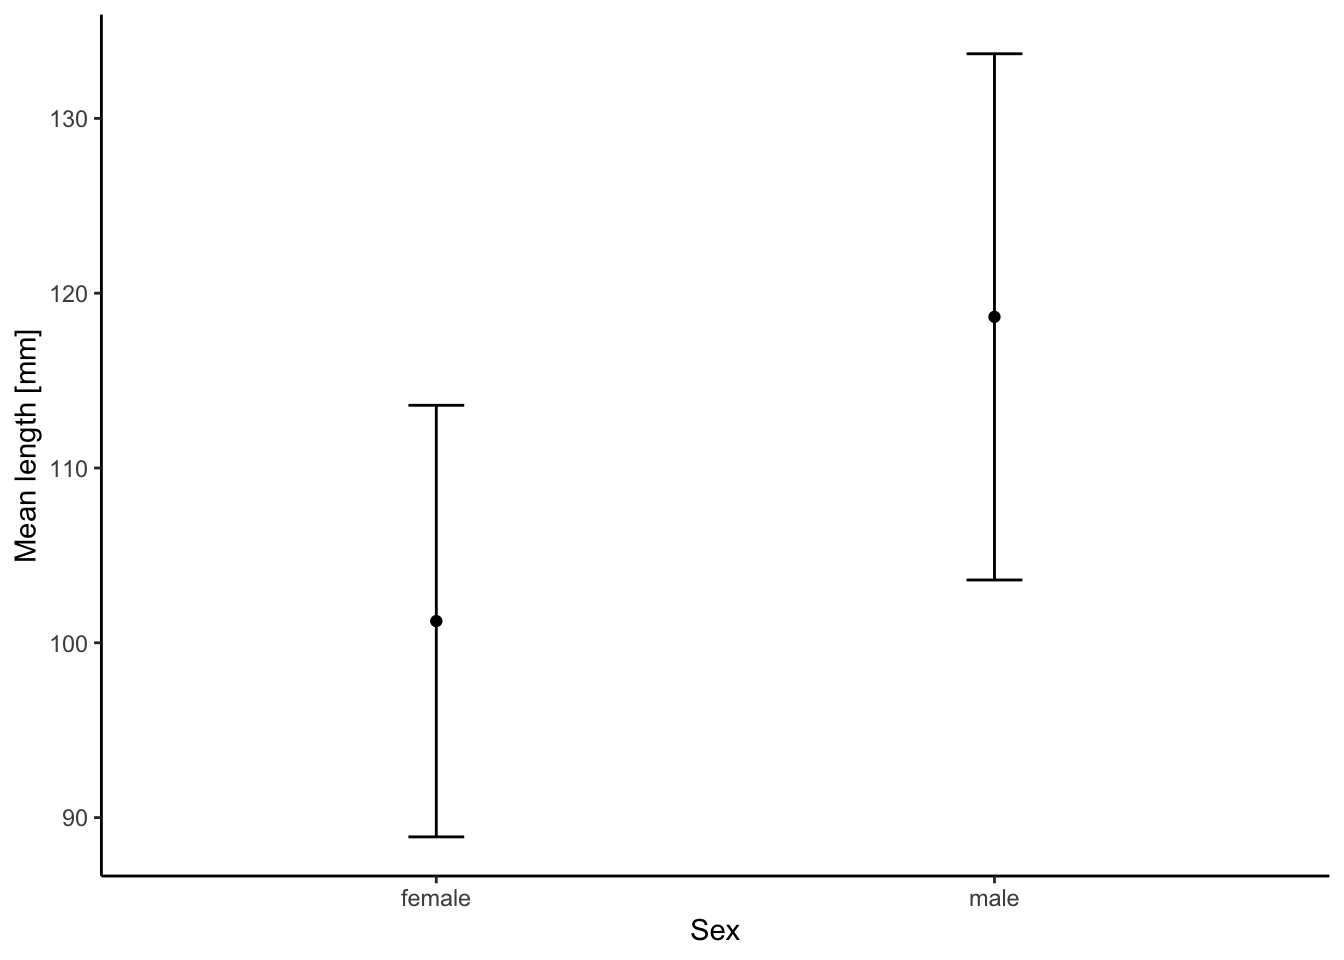
\includegraphics{Primer2Evolution_files/figure-latex/meanplot-1.pdf}

\hypertarget{reflection-questions-1}{%
\section{Reflection Questions}\label{reflection-questions-1}}

\begin{enumerate}
\def\labelenumi{\arabic{enumi}.}
\tightlist
\item
  There is phenomenal variation in human height. The graph below shows variation among over 80 human populations (countries; in different colors) and across time (from 1897 to 1996). As you can see, there is a spread of about 20 cm in mean height among populations that has persisted through time. In addition, mean height has increased by an average of \textasciitilde8 cm over 100 years (black line). Do you think the variation in height among the populations and the change through time are the product of evolution? Why? If you want to explore these data further, you can download them \href{data/human_height.csv}{here}. Data was originally retrieved from \href{https://ourworldindata.org/human-height}{\emph{Our World in Data}} (\href{https://creativecommons.org/licenses/by/4.0/}{CC BY 4.0}).
\end{enumerate}

\begin{figure}
\centering
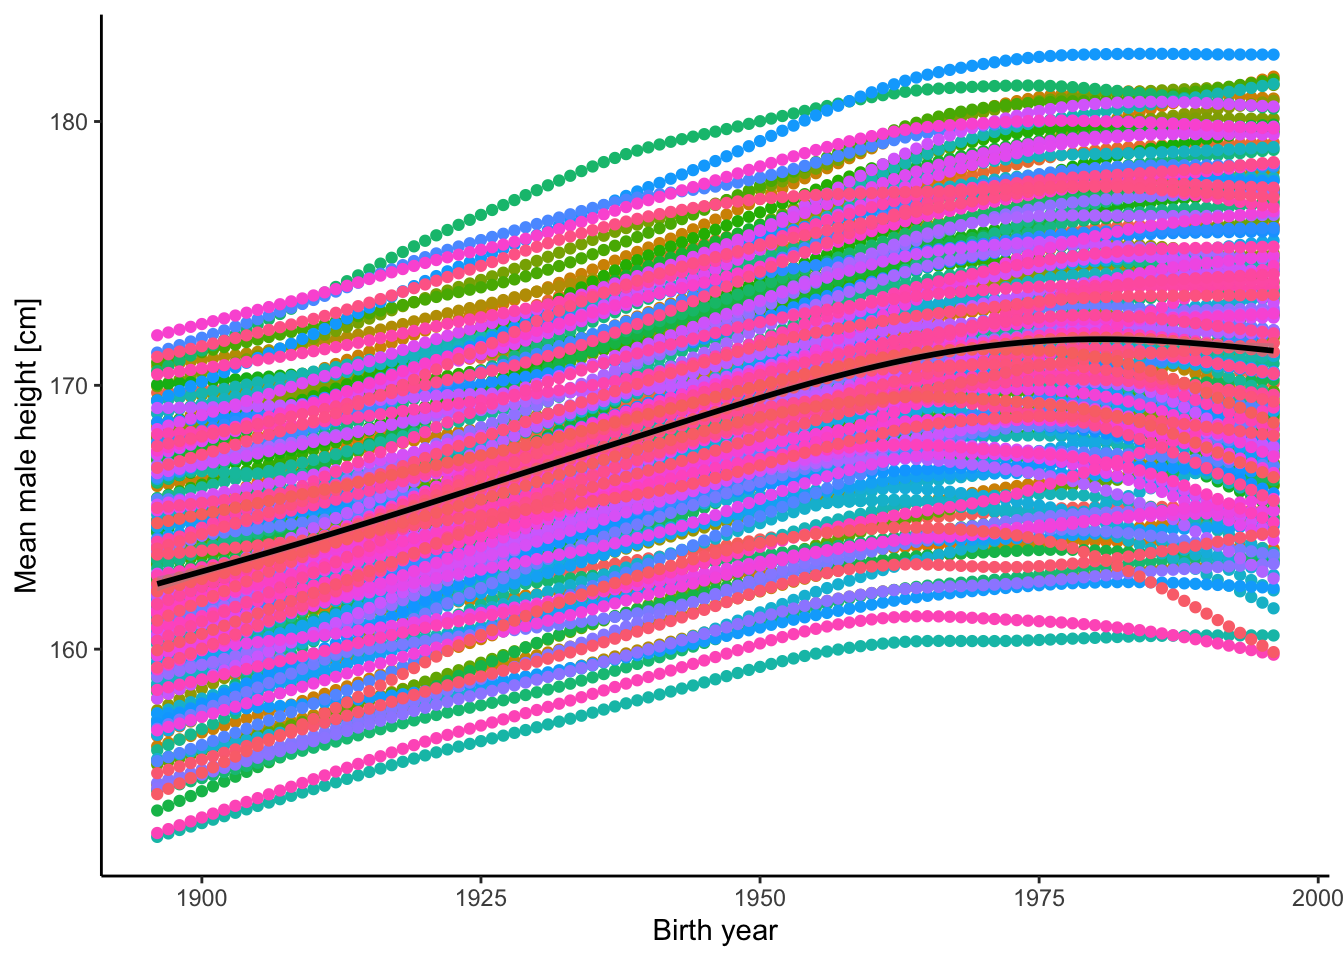
\includegraphics{Primer2Evolution_files/figure-latex/humansize-1.pdf}
\caption{\label{fig:humansize}Mean height of male humans in different countries (by color) and across years.}
\end{figure}

\begin{enumerate}
\def\labelenumi{\arabic{enumi}.}
\setcounter{enumi}{1}
\tightlist
\item
  The evidence for speciation discussed in this chapter hinged on a specific definition of speciation. What do you think are some of the disadvantages of that specific definition?
\item
  Transitional fossils are a hallmark of evolution. However, we lack transitional fossils between many groups of organisms, especially between phyla that arose during the Cambrian explosion. Why do you think this is? How does this undermine evolutionary theory?
\end{enumerate}

\hypertarget{references-2}{%
\section{References}\label{references-2}}

\begin{itemize}
\item
  Carroll, SP, AP Hendry, DN Reznick, CW Fox (2007). \href{https://besjournals.onlinelibrary.wiley.com/doi/full/10.1111/j.1365-2435.2007.01289.x}{Evolution on ecological time-scales}. \emph{Functional Ecology} 21, 387--393.
\item
  Daeschler, EB, NH Shubin, FA Jenkins Jr.~(2006). \href{https://www.nature.com/articles/nature04639}{A Devonian tetrapod-like fish and the evolution of the tetrapod body plan}. \emph{Nature} 440, 757--763.
\item
  Darwin, C. (1859). \href{https://www.biodiversitylibrary.org/item/122307\#page/7/mode/1up}{\emph{On the origin of species based on natural selection, or the preservation of favoured races in the struggle of life}}. John Murray.
\item
  Friedberg, F, AR Rhoads (2000). \href{https://pubmed.ncbi.nlm.nih.gov/10877945/}{Calculation and verification of the ages of retroprocessed pseudogenes}. \emph{Molecular Phylogenetics and Evolution} 16, 127--130.
\item
  Hairston Jr, NG, SP Ellner, MA Geber, T Yoshida, JA Fox (2005). \href{https://onlinelibrary.wiley.com/doi/full/10.1111/j.1461-0248.2005.00812.x}{Rapid evolution and the convergence of ecological and evolutionary time}. \emph{Ecology Letters} 8, 1114--1127.
\item
  Hendry, AP, CL Peichel, B Matthews, JW Boughman, P Nosil (2013). \href{http://www.evolutionary-ecology.com/open/ccar2833.pdf}{Stickleback research: the now and the next}. \emph{Evolutionary Ecology Research}, 15, 111--141.
\item
  Irwin, DE, S Bensch, JH Irwin, TD Price (2005). \href{https://science.sciencemag.org/content/307/5708/414}{Speciation by distance in a ring species}. \emph{Science} 307, 414--416.
\item
  Jones, FC, MG Grabherr, YF Chan, P Russell, E Mauceli, J Johnson, \ldots{} DM Kingsley (2012). \href{https://www.nature.com/articles/nature10944}{The genomic basis of adaptive evolution in threespine sticklebacks}. \emph{Nature} 484, 55--61.
\item
  Krishnan, J, N Rohner (2017). \href{https://royalsocietypublishing.org/doi/10.1098/rstb.2015.0487}{Cavefish and the basis for eye loss}. \emph{Philosophical Transactions of the Royal Society of London B} 372, 20150487.
\item
  Laurentino, TG, D Moser, M Roesti, M Ammann, A Frey, F Ronco, B Kueng, D Berner (2020). \href{https://www.nature.com/articles/s41467-020-15657-3}{Genomic release-recapture experiment in the wild reveals within-generation polygenic selection in stickleback fish}. \emph{Nature Communications} 11, 1928.
\item
  Lescak, EA, SL Bassham, J Catchen, O Gelmond, ML Sherbick, FA von Hippel, WA Cresko (2015). \href{https://www.pnas.org/content/112/52/E7204}{Evolution of stickleback in 50 years on earthquake-uplifted islands}. \emph{Proceedings of the National Academy of Sciences USA} 112, E7204--E7212.
\item
  Marth, JD (2008). \href{https://www.nature.com/articles/ncb0908-1015}{A unified vision of the building blocks of life}. \emph{Nature Cell Biology} 10, 1015--1016.
\item
  Nosil, P (2007). \href{https://www.journals.uchicago.edu/doi/abs/10.1086/510634}{Divergent host plant adaptation and reproductive isolation between ecotypes of \emph{Timema} \emph{cristinae} walking sticks}. \emph{American Naturalist} 169, 151--162.
\item
  Ostrom, JH (1976). \href{https://onlinelibrary.wiley.com/doi/abstract/10.1111/j.1095-8312.1976.tb00244.x}{\emph{Archaeopteryx} and the origin of birds}. \emph{Biological Journal of the Linnean Society. Linnean Society of London} 8, 91--182.
\item
  Pereira, RJ, WB Monahan, DB Wake (2011). \href{https://bmcecolevol.biomedcentral.com/articles/10.1186/1471-2148-11-194}{Predictors for reproductive isolation in a ring species complex following genetic and ecological divergence}. \emph{BMC Evolutionary Biology} 11, 194.
\item
  Woodburne, MO, WJ Zinsmeister (1982). \href{https://science.sciencemag.org/content/218/4569/284}{Fossil land mammal from Antarctica}. \emph{Science} 218, 284--286.
\end{itemize}

\hypertarget{a-mechanism-for-change}{%
\chapter{A Mechanism for Change}\label{a-mechanism-for-change}}

Darwin's core contribution to science was not just his assemblage of evidence for the pattern of evolution (\href{evidence-for-evolution.html}{Chapter 2}), but also the conception of a mechanism that could explain such patterns: natural selection. In doing so, he formalized an idea that humans have used for millennia to shape traits of agricultural crops, livestock, and companion animals. If you weed out the duds and promote the variants you desire, you end up with giant potatoes, hens that lay over 300 eggs a year, pigs that produce the most scrumptious bacon, and the most adorable puppies that steal your well-bred breakfast.

Humans have been domesticating plants and animals for various purposes for over 10,000 years, thereby shaping their evolution. The recipe for success was relatively simple: assess the traits of individuals in your stock, choose the ones with the desired traits for breeding, and keep doing just that, time and time again. While we---as humans---have a long history of selective breeding, it does not actually take that much time for artificial selection to have profound effects. The speed at which we can domesticate animals was illustrated by an experiment that aimed to better understand the evolution of dogs from wolves by selectively breeding foxes.

In 1959, Lyudmila Trut and Dmitri Belyaev started to selectively breed silver foxes (\emph{Vulpes vulpes}) in a Russian fur farm (Dugatkin 2018). Breeders were selected based on their tameness. Foxes that were curious toward humans were retained, while those that were shy or even aggressive\ldots{} well, they became coats for the Russian elite. Over a few decades, foxes in this experiment not only became tamer and tamer, but they also exhibited changes in a variety of other traits: their facial structure diverged, some exhibited floppy ears and curly tails, their coat colors changed, and some even started to make novel sounds (seriously\ldots{} read about \href{https://www.amazon.com/Pushinka-Barking-Fox-Unexpected-Friendship/dp/1943978468}{\emph{Pushinka the Barking Fox}}\textbf{)}. Today, the foxes of this experiment still contribute to fur production, but you can also buy domesticated foxes as pets, even here in the United States. Selection on an apparently simple trait (tamness) lead to complex changes in the fox population in just a few decades.

Explore More

To learn about the famous fox experiment, check out \href{https://www.amazon.com/How-Tame-Fox-Build-Dog/dp/022659971X}{\emph{How to Tame a Fox (and Build a Dog): Visionary Scientists and a Siberian Tale of Jump-Started Evolution}} by Lee Dugatkin and Lyudmila Trut.

Darwin, through his experience with pigeon breeding, was not only aware of the power of selective breeding and domestication, but he was also able to relate that process to the patterns of evolutionary change he observed in nature. This chapter will take you through Darwin's logic of natural selection.

\hypertarget{darwins-logic}{%
\section{Darwin's Logic}\label{darwins-logic}}

Natural selection explains evolution based on first principles; deceivingly simple and equally powerful. Darwin made four key observations, also know as Darwin's postulates:

\begin{enumerate}
\def\labelenumi{\arabic{enumi}.}
\item
  Individuals in a population vary in their traits.
\item
  Some of that trait variation is inherited from parents to their offspring.
\item
  More offspring are produced in every generation than can possibly survive.
\item
  Successful survival and reproduction of those offspring is not random but dependent on the traits they inherited from their parents.
\end{enumerate}

If these four observations hold true, then the consequence is that the heritable traits that impact survival and reproduction will change from one generation to the next. Beneficial variants will become more common through time, ultimately causing adaptation to the prevailing environmental conditions.

While we intuitively know at least some of Darwin's postulates to be true, we should treat them all as hypotheses. We cannot only test whether the predictions of each postulate hold up, but we can also empirically test whether evolutionary change is really the consequence of the four postulates. In the following sections, we will take a closer look at the four postulates and discuss an actual case study of natural selection in the wild, building on what you learned about Darwin's finches in the last chapter.

\hypertarget{variation}{%
\subsection{Variation}\label{variation}}

Individuals in a population vary in their traits. We know this to be true in humans; if you just look around the classroom, inter-individual differences become evident in many traits. While nearly all humans have one head, two eyes and ears, and five digits on each limb, we vary in body size, the relative proportions of morphological traits, the color of our skin, hair, and eyes, aspects of our physiology, as well as behavioral traits that make up our personalities. If you have ever cared for pets or plants in a garden, you will have some intuition about trait variation in those species, too.

From a practical perspective, the question is not so much \emph{whether} individuals in a population vary, but which variable traits are actually important from a functional perspective. In other words, what traits should we actually be paying attention to as evolutionary biologists? For example, some humans have hair on their phalanges and some don't. Does that matter? Probably not\ldots{} This is where careful natural history observations come into play. To ask meaningful questions about evolution in natural systems, we have to consider organisms as holistic entities consisting of interacting traits in the context of the abiotic and biotic factors comprising their environment. So before going out into natural populations and quantifying variation, we want to formulate concrete hypotheses about the role of specific traits in shaping organismal performance in terms of survival and reproduction.

Once relevant traits for study have been identified, quantifying actual trait variation is not too difficult. It is amazing what ground-breaking data sets were collected merely using a caliper. But depending on the nature of a trait, any other method might be used to quantify inter-individual differences, from the molecular composition of cells all the way up to behavioral responses. Variation of traits among individuals in a population is typically visualized using frequency histograms (like in Figure \ref{fig:beaksizevariation}), and most traits in natural populations exhibit a normal distribution, where most individuals have intermediate trait values, and extreme trait values are more rare. We will explore why this is in \href{the-evolution-of-quantitative-traits.html}{Chapter 8}.

Ultimately, any variation we can observe and quantify in a population represents the raw material of evolution. Selection can act on variable traits, potentially causing evolutionary change---if said trait is heritable. If there is no variation, there can be no selection and accordingly no evolution, no matter how heritable a trait is.

\hypertarget{heritability}{%
\subsection{Heritability}\label{heritability}}

Once variation in a potentially interesting trait is quantified, we have to test whether trait variation is heritable. Many---if not all---quantitative traits are not only shaped by genes inherited by the parents, but also by environmental factors. For example, a child's potential to grow tall is dependent on whether their parents were tall (\emph{i.e.}, variation in genes that mediate growth) as well as adequate access to resources during the critical times in development. Similarly, the expression of certain colors in insects, fish, and birds is dependent on access to nutritional precursors and the genetically determined physiological capacity to turn those precursors into pigments deposited in tissues. Genetic and environmental effects work together to shape the variation of traits that we observe. So how can we determine the relative contribution of each?

Heritability measures the degree to which variation in a trait \emph{in a population} is due to genetic variation. Thus, it is not a metric we can establish for a particular individual or a particular family; rather, we need to quantify the correspondence of parent and offspring traits across multiple families in a population. We can then plot offspring trait values as a function of their parents' trait values and calculate regression lines. The slope of those parent-offspring regressions is a measure of heritability (in particular, narrow-sense heritability, but we will learn more about this in \href{the-evolution-of-quantitative-traits.html}{Chapter 8}). If the slope of the parent-offspring regression is close to one, it means there is almost perfect correspondence between parent and offspring traits, and heritability is high (blue line in Figure \ref{fig:herit}). If the slope of the line is close to zero, there is no correspondence between parent and offspring traits; in this case, phenotypic variation is entirely shaped by environmental influences, and there is no heritability (green line in Figure \ref{fig:herit}). Any slopes between zero and one (like the orange line in Figure \ref{fig:herit}) indicate that genetic and environmental factors both contribute to shaping trait variation in a population.

\begin{figure}
\centering
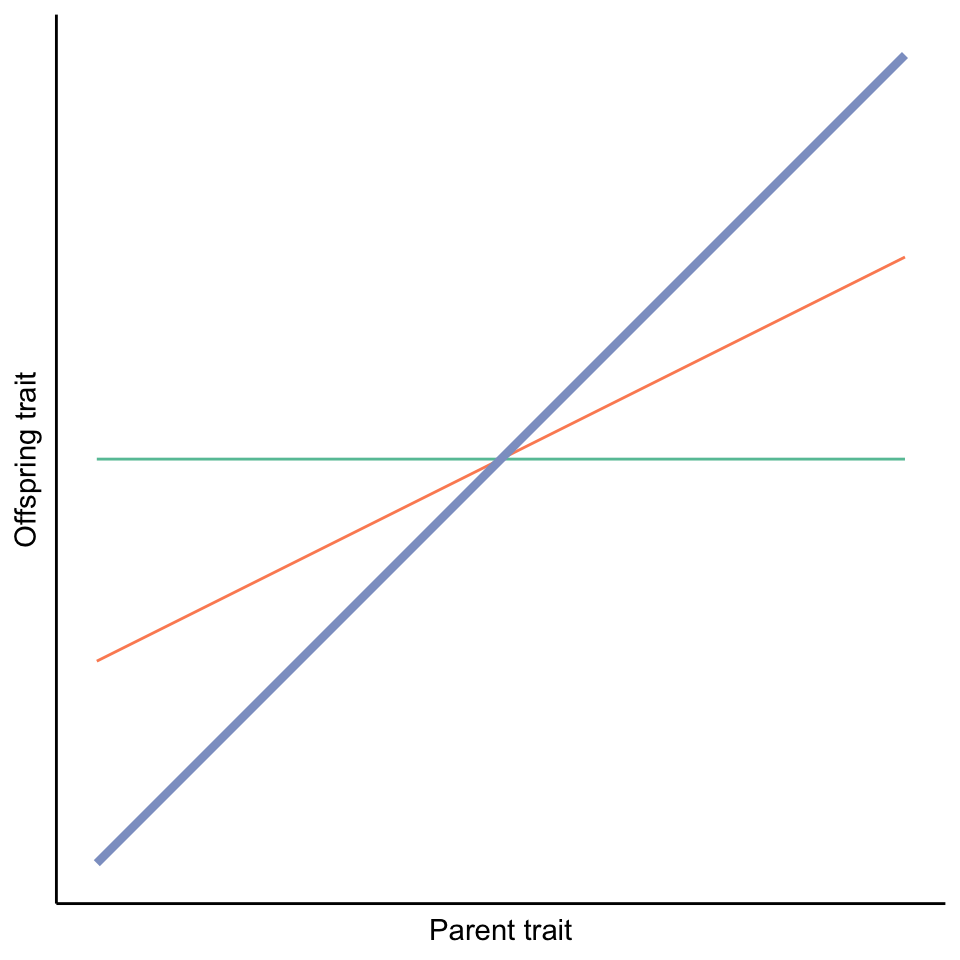
\includegraphics{Primer2Evolution_files/figure-latex/herit-1.pdf}
\caption{\label{fig:herit}The slope of parent-offspring regressions reveal the degree of heritability. A slope of one indicates high heritability (blue line), while a slope of zero indicates no heritability (orange line). Intermediate slopes indicate that genetic and environmental effects both impact trait variation in a population.}
\end{figure}

Just like variation is required for there to be selection, heritability is required to translate selection into evolutionary change. If there is no heritability in a trait, it cannot evolve. Evolutionary change in a trait is consequently not only shaped by selection, but also by the degree to which the trait is heritable.

\hypertarget{the-struggle-for-existence}{%
\subsection{The Struggle for Existence}\label{the-struggle-for-existence}}

All organisms have the potential to produce more offspring than required to replace themselves. Hence, all populations have the potential for exponential growth. We see evidence for such exponential growth whenever we inoculate a Petri dish with bacteria, when invasive species are introduced into a new area, or when pathogens spread through a population of susceptible hosts. But eventually, exponential growth comes to an end when resources get more scarce and competition intensifies. Nutrients on the agar will dwindle, invasives gradually encroach on all available spaces, and hosts either die off or develop immunity. Resource limitation and competition ultimately stifle exponential growth, and thus, natural population growth is typically density-dependent, which can be described using logistic growth cruves. During logistic growth, a carrying capacity sets the threshold beyond which positive population growth becomes impossible, because the resources to sustain additional population growth are not available.

Darwin was not the first to recognize the relationship between population growth and resource availability. In fact, he was inspired by an earlier economist, Thomas Malthus, who voiced concerns in the late 1700s about the growth of agricultural food production lagging behind human population growth. Although the industrial and agricultural revolutions proved Malthus wrong (global food production largely kept pace with human population growth), he was right about one thing: the growth of any population can only continue if its resources grow as well. Hence, most natural populations remain relatively stable through time despite the potential for exponential population growth (Figure \ref{fig:elephants}), aside from comparatively minor fluctuations across seasons and years.

\begin{figure}
\centering
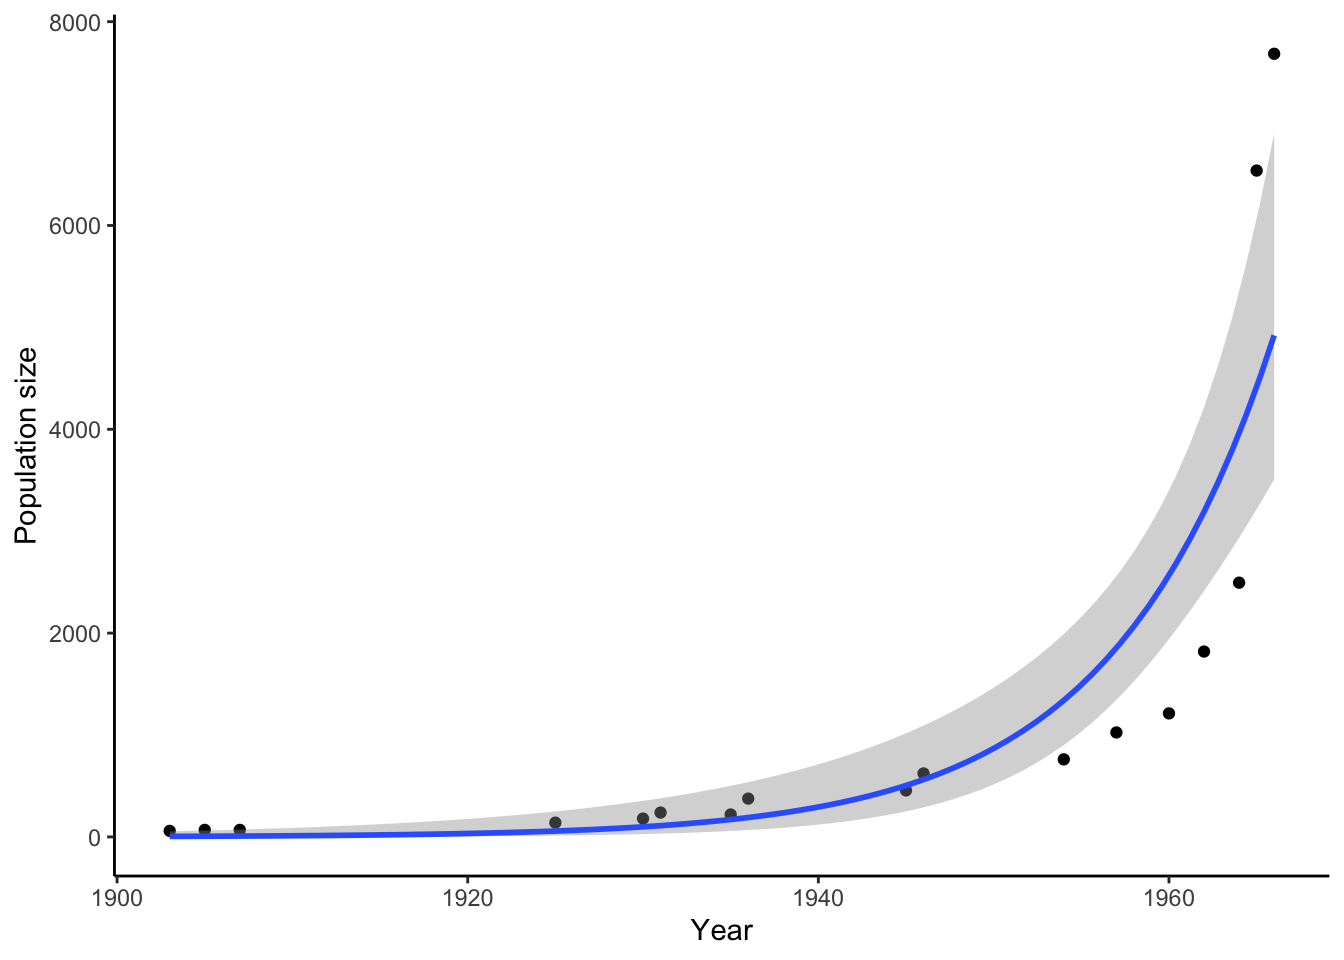
\includegraphics{Primer2Evolution_files/figure-latex/elephants-1.pdf}
\caption{\label{fig:elephants}Even animals with slow reprodictive rates have the potential for exponential growth. Depicted is the population size of African elephants in Kruger National Park, South Africa, after they were protected from hunting.}
\end{figure}

So where do all the extra offspring go? They die! Most individuals born succumb to a lack of resources, predators, or diseases long before they reach sexual maturity, and only a small fraction of offspring born in any generation survive long enough to reproduce. The consequence of this overproduction is fierce competition in every generation. This competition is what Darwin referred to as the struggle for existence. Natural selection is often particularly intense in populations that are close to their carrying capacity and in populations that are contracting.

\hypertarget{non-random-survival-and-reproduction}{%
\subsection{Non-Random Survival and Reproduction}\label{non-random-survival-and-reproduction}}

Darwin's final proposition was that winners and losers in the struggle for existence are not determined by chance. Instead, specific traits and trait combinations lead to a higher probability of survival and reproduction. In a landscape plagued by drought, it is the plant with the deepest roots that has the best chance of persisting. In an stream rich in predators, the fish with the fastest escape response is most likely to dodge imminent attacks. In a forest with limited food resources, the parrot with the most efficient foraging strategy can garner enough food resources to produce and feed a clutch of young. Depending on the challenge at hand, individuals with specific traits or trait combinations will have a slight advantage over others.

Importantly, natural selection is not random. That does not mean natural selection is guided by conscious intent, as sometimes is insinuated. Rather, natural selection just happens because some variants have a disproportionate likelihood to survive and reproduce. As a consequence of natural selection's non-random nature, evolution by natural selection increases adaptation from one generation to the next.

A concept related to natural selection is fitness, which is used to describe the strength of natural selection on different variants. Fitness in biology is not a measure of an individual's physical prowess or health, but rather the relative contribution of a particular phenotype to the gene pool of the next generation.

Definition: Fitness

Fitness quantifies individual reproductive success and represents the average contribution to the gene pool of the next generation by individuals of the specified phenotype in a given environment.

Fitness is relative in the sense that it is typically expressed for one phenotype in relation to another. For example, the fitness of mouse with a dark fur coat is higher relative to the fitness of a mouse with a light fur coat, because the darker coat color increases crypsis against the dark leaf litter of the forest habitat. Fitness is also context-dependent, and the relative fitness of two phenotypes may change depending on the environmental conditions. For example, in a mouse population inhabiting beaches, the light colored phenotype may have higher fitness, because it is better camouflaged against the light sand.

\hypertarget{putting-darwins-logic-to-the-test}{%
\section{Putting Darwin's Logic to the Test}\label{putting-darwins-logic-to-the-test}}

The core strength of Darwin's postulates is that they can be treated as hypotheses, and we can use data from natural populations to test whether evolution by natural selection is happening. In this section, we will once again retrace the steps of Rosemary and Peter Grant. In \href{evidence-for-evolution.html}{Chapter 2}, you explored their data on beak size variation of the \emph{Geospiza fortis} population on Daphne Major Island (Figure \ref{fig:timeseries}). During a massive drought associated with an El Niño in 1977, there was a substantial increase of beak size over a short period of time. But does this change represent an evolutionary change caused by natural selection? If so, we would predict (1) observable variation in beak size in the \emph{G. fortis} population, (2) that some of the beak size variation is heritable, (3) that the finches on Daphne Major are in fact facing a struggle for existence, and (4) that survival in the finch population is not random but related to beak size. Last but not least, we would also predict differences in beak size across generations.

\begin{figure}
\centering
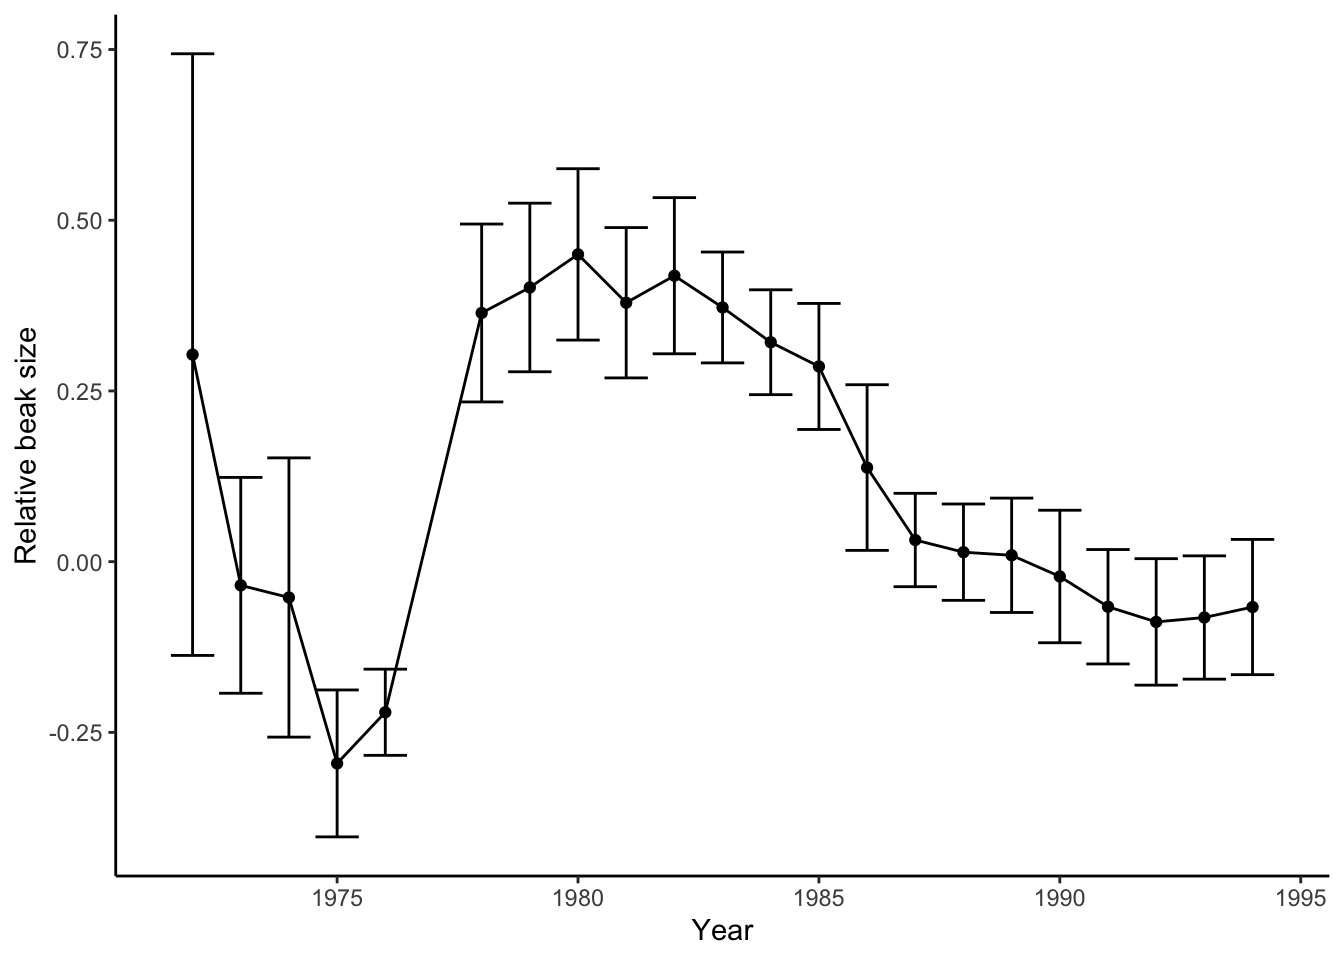
\includegraphics{Primer2Evolution_files/figure-latex/timeseries-1.pdf}
\caption{\label{fig:timeseries}Variation of relative beak size in \emph{G. fortis} on Daphne Major Island from 1972-1995. Positive numbers indicate larger beaks and negative number represent smaller beaks.}
\end{figure}

\hypertarget{is-there-variation-in-beak-size}{%
\subsection{Is there Variation in Beak Size?}\label{is-there-variation-in-beak-size}}

To test whether there is variation in beak size within the \emph{G. fortis} population, we can use a frequency histogram to plot raw beak size data collected by the Grants (Figure \ref{fig:beaksizevariation}). As with most quantitative traits, beak size variation follows a normal distribution, with most individuals exhibiting intermediate beak sizes around 9.5 mm. However, the spread in beak sizes is vast; the smallest beaks measured just 6 mm, and the largest ones almost 14 mm. That is more than a two-fold spread! Therefore, there is clear variation in beak size that natural selection could potentially act upon; \emph{i.e.}, we found evidence for Darwin's first postulate.

\begin{figure}
\centering
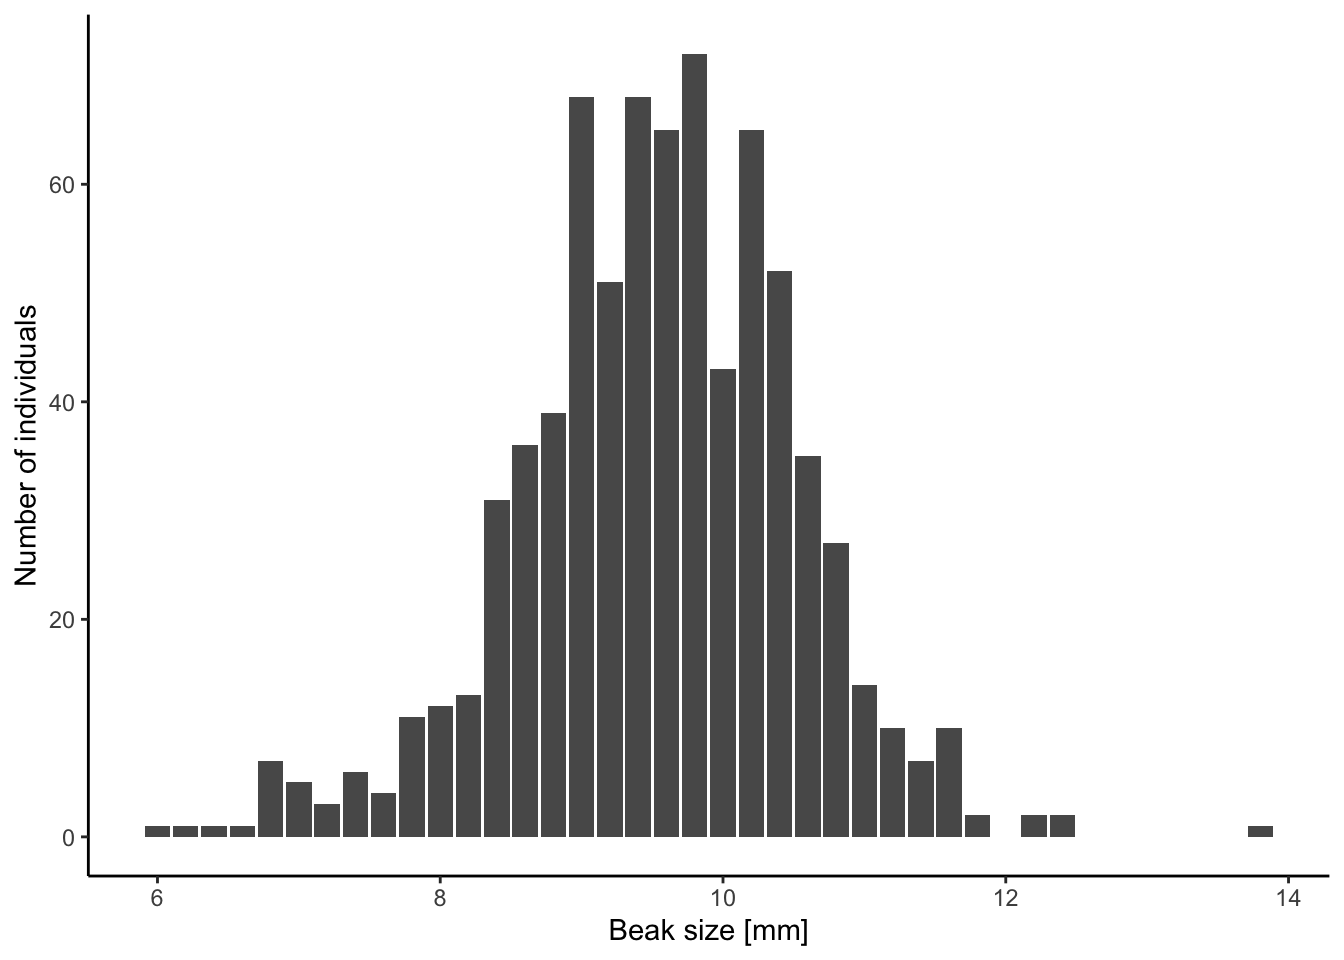
\includegraphics{Primer2Evolution_files/figure-latex/beaksizevariation-1.pdf}
\caption{\label{fig:beaksizevariation}Frequency histogram showing beak size variation in the \emph{G. fortis} population before the drought in 1976. \href{data/3_beak_size_variation.csv}{Data} from Boag and Grant (1984).}
\end{figure}

\hypertarget{is-variation-in-beak-size-heritable}{%
\subsection{Is Variation in Beak Size Heritable?}\label{is-variation-in-beak-size-heritable}}

To test whether beak size is heritable, the Grants tracked the development of individuals by banding them with unique markers and comparing beak sizes of parents and their adult offspring. Plotting the average beak size of each parental pair against the average beak size of their offspring reveals a clear positive relationship between the two variables, both for families studied in 1976 and 1978 (Figure \ref{fig:heritability}). Parents with large beaks tended to raise chicks with large beaks, and parents with small beaks had chicks with small beaks. The slope of the regression lines for both years is almost 0.9, indicating a high heritability. So, beak size is not only variable but also highly heritable, providing evidence for Darwin's second postulate.

\begin{figure}
\centering
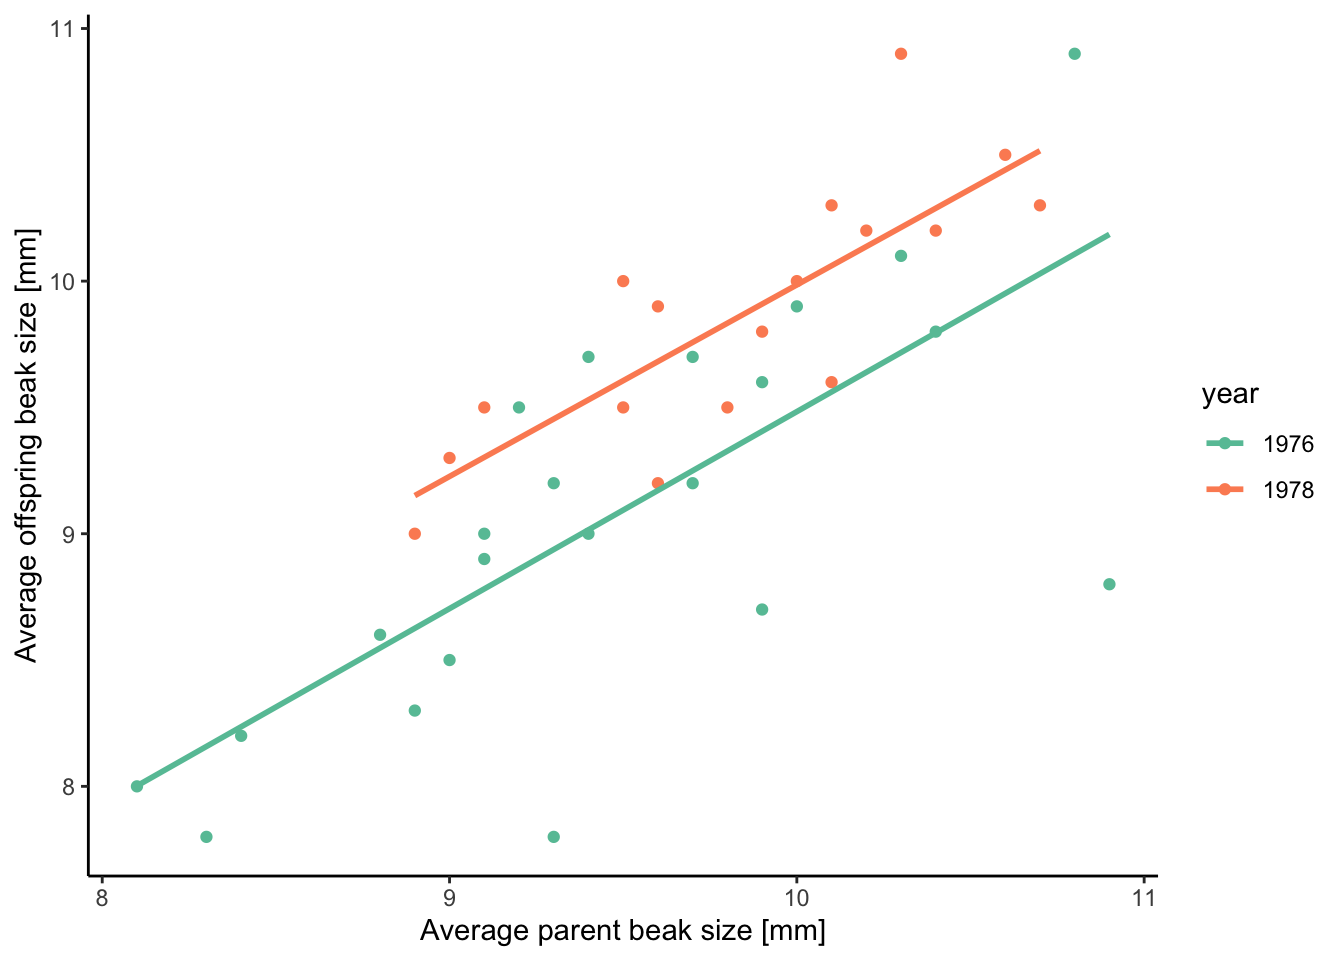
\includegraphics{Primer2Evolution_files/figure-latex/heritability-1.pdf}
\caption{\label{fig:heritability}Scatter plot showing the relationship between the beak size of the parents (average between mother and father) and their offspring (average across multiple siblings) measured separately in 1976 and 1978. \href{data/3_parent_offspring.csv}{Data} from Boag (1983).}
\end{figure}

\hypertarget{is-there-a-struggle-for-existence}{%
\subsection{Is there a Struggle for Existence?}\label{is-there-a-struggle-for-existence}}

As with any population that has a capacity for exponential growth and is trapped in a small area, the struggle for existence in Darwin's finches seems obvious, but election can be particularly strong when conditions are harsh and populations are contracting. Throughout the 1977 drought, finch populations on Daphne Major crashed from about 1,500 birds in March 1976 to to less than 200 birds in late 1977 (Figure \ref{fig:popsize}). This represents a decline of over 85 \% in less than two years. The Grants were able to show that this decline was primarily related to a limitation of food resources, as the lack of significant precipitation limited plant growth and seed production on the island. Consequently, the Grants witnessed struggle for existence first hand, finding support of Darwin's third postulate.

\begin{figure}
\centering
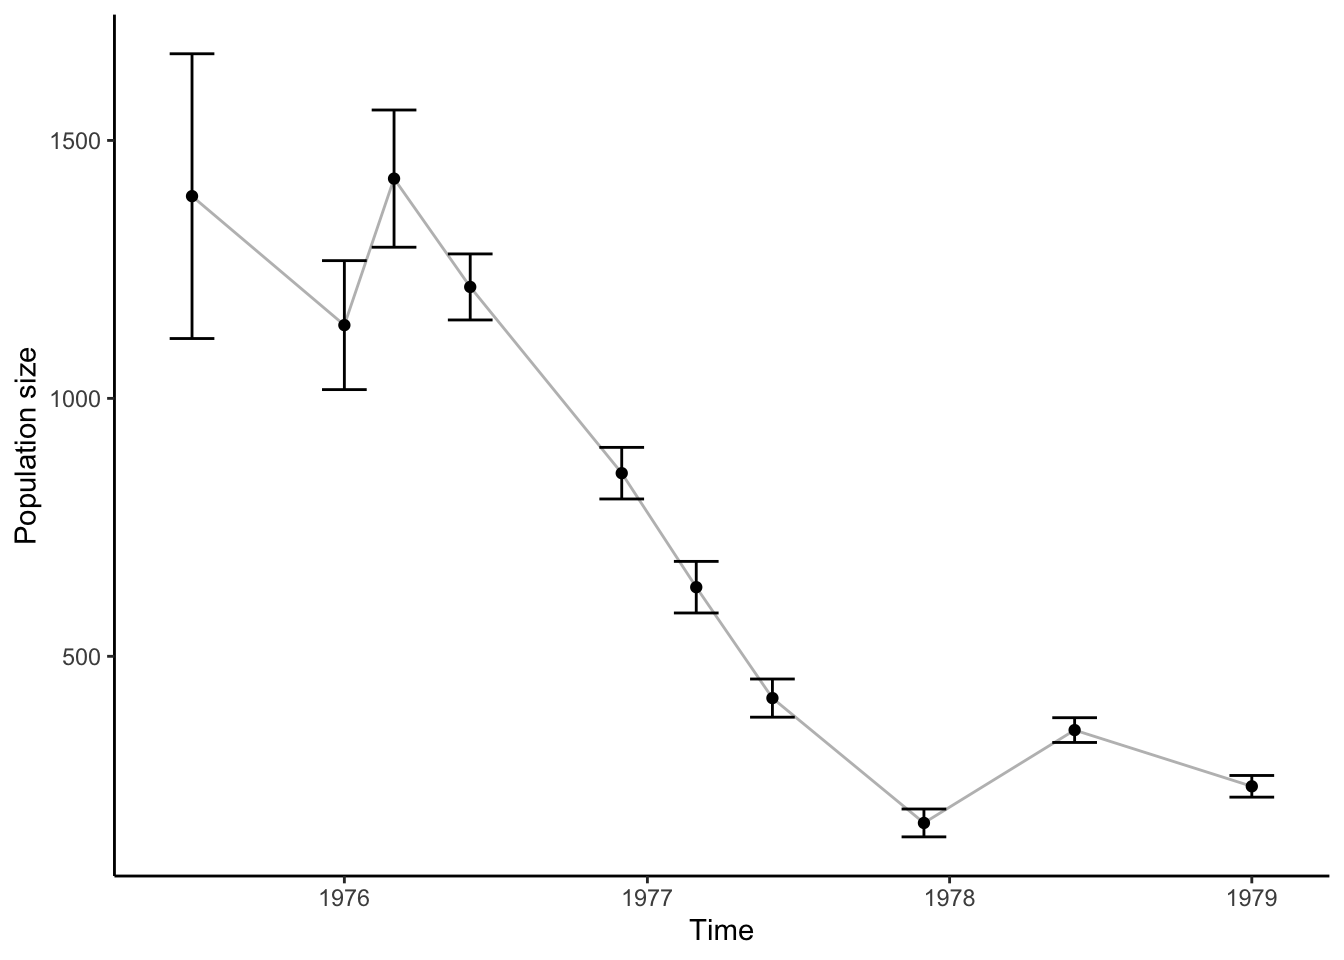
\includegraphics{Primer2Evolution_files/figure-latex/popsize-1.pdf}
\caption{\label{fig:popsize}Population size of \emph{G. fortis} on Daphne Major between July 1975 and January 1979. \href{data/3_population_size.csv}{Data} from Boag and Grant (1981).}
\end{figure}

\hypertarget{is-survival-non-random}{%
\subsection{Is Survival Non-Random?}\label{is-survival-non-random}}

To test whether survival of birds was non-random in relation to beak size, we can compare the beak size distribution in individuals before the drought in 1976 and the birds that were left after the drought in 1978. As you can see in Figure \ref{fig:survival}, surviving birds on average had a larger beak size than individuals prior to the selection event. The Grants were also able to explain exactly why a larger beak size conferred a selective advantage. As the drought progressed, there was not only a decline in seed abundance, but the average seed also became larger and harder, because the smaller and softer seeds were eventually all eaten up by the finches. As seed quality changed, finches with larger beaks had a foraging advantage, because they were able to open larger and harder seeds more effectively. The disproportionate survival of individuals with larger beaks provides clear evidence for Darwin's fourth postulate.

\begin{figure}
\centering
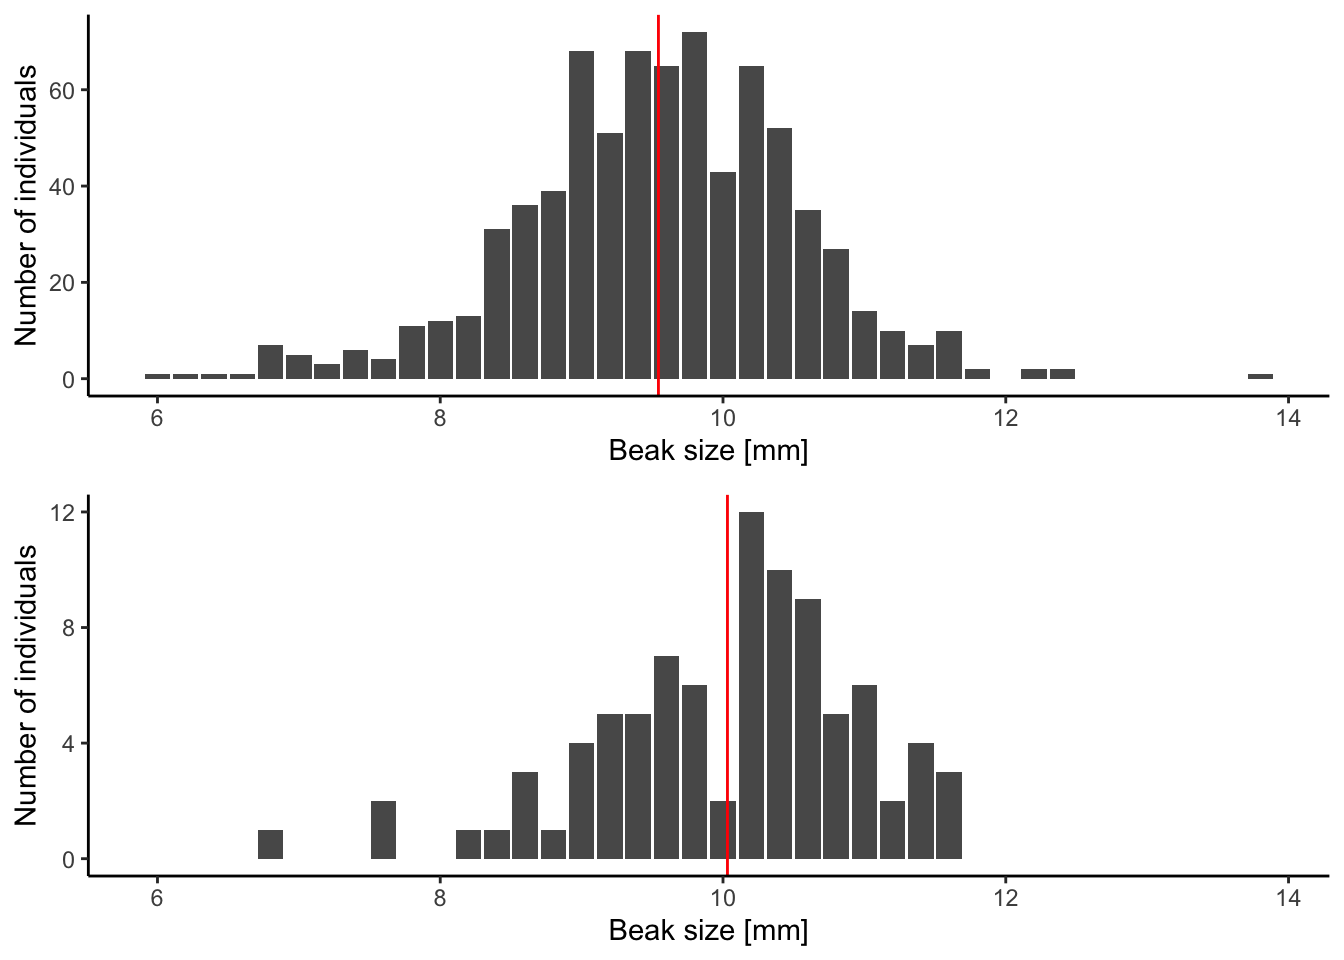
\includegraphics{Primer2Evolution_files/figure-latex/survival-1.pdf}
\caption{\label{fig:survival}Frequency histograms showing beak size variation in the finch population before the drought (top) and in the surviving individuals after the drought (bottom). The vertical red lines represent the mean beak size in each set. The beak size of the average survivor was slightly higher than the population average prior to the drought, indicating that natural selection happened. \href{data/3_beak_size_variation.csv}{Data} from Boag and Grant (1984).}
\end{figure}

\hypertarget{did-non-random-survival-lead-to-evolution}{%
\subsection{Did Non-Random Survival Lead to Evolution?}\label{did-non-random-survival-lead-to-evolution}}

At this stage, we have shown heritable variation in beak size, strong selection caused by a massive drought, and non-random survival associated with beak size. However, we have not yet shown that evolution has occurred. We have only shown the action of natural selection. But testing the hypothesis of evolutionary change requires the documentation of changes across generations, not just differential survival within generations. To do so, we can can compare the beak size of offspring born before the drought (1976) to the beak size of offspring both after the drought (in 1978; these are the offspring of the survivors). As expected, based on the high heritability of beak size, we see that the average offspring in 1978 exhibited a larger beak than the average offspring in 1976 (Figure \ref{fig:evolutionarychange}).

Taken together, these data sets conclusively show that the drastic change in beak size from 1976 to 1978 (Figure \ref{fig:timeseries}) represents evolution by natural selection. The finch population adapted to a new reality, where the average food source was larger and harder. The Grants' pioneering work linked an evolutionary pattern that they observed to a concrete mechanism that explained the pattern; they documented the interplay of pattern and process in a naturally evolving population.

\begin{figure}
\centering
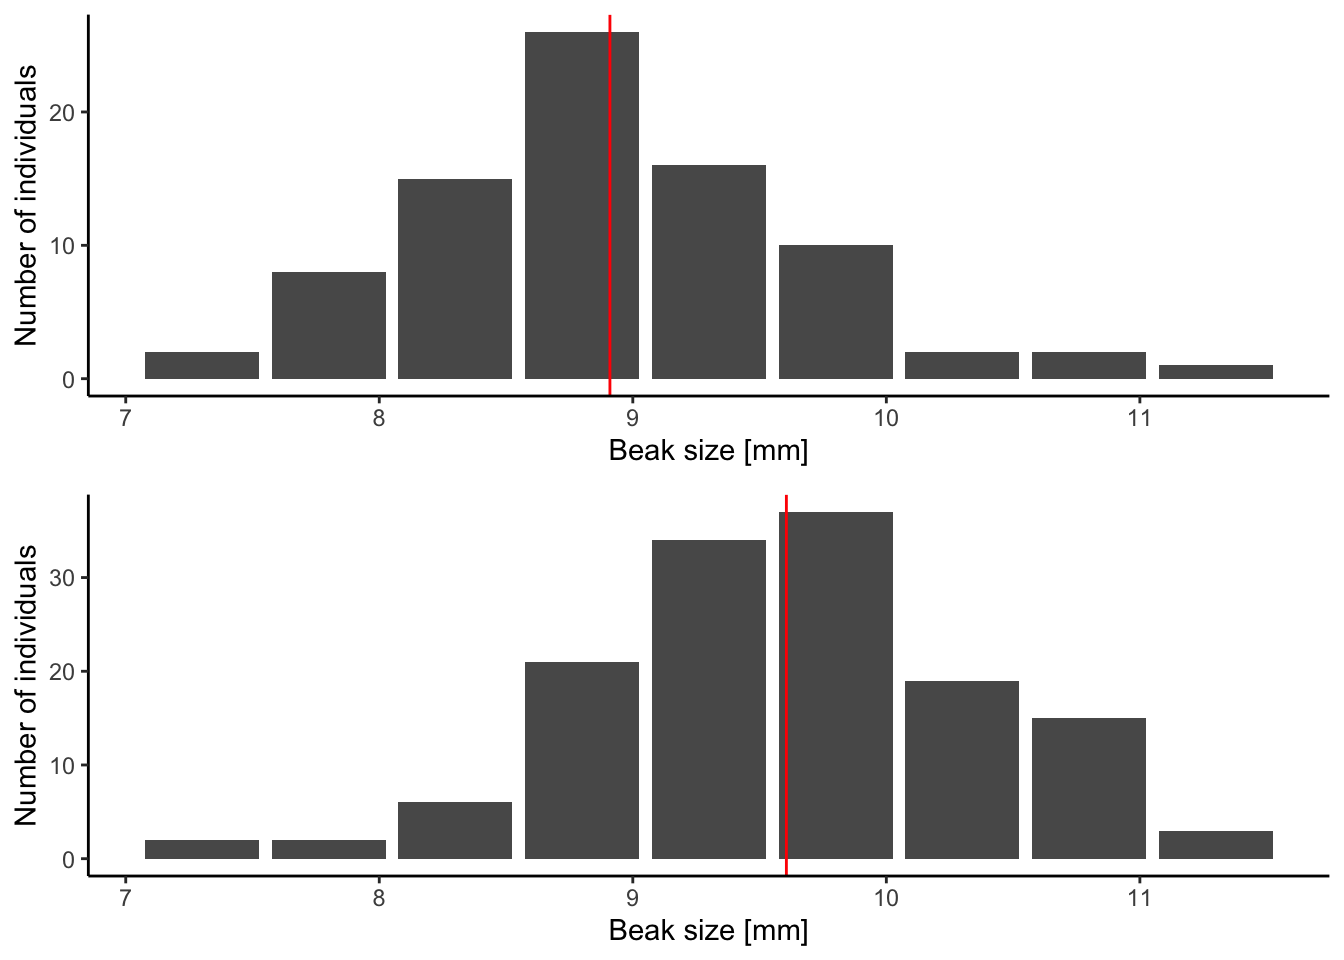
\includegraphics{Primer2Evolution_files/figure-latex/evolutionarychange-1.pdf}
\caption{\label{fig:evolutionarychange}Frequency histograms showing beak size variation in the finch offspring born before the drought (top) and after the drought (bottom). The vertical red lines represent the mean beak size in each set. The beak size of the average offspring born after the selection event was higher than the offspring average prior, indicating that evolution happened. \href{data/3_offspring_beaks.csv}{Data} from Grant and Grant 2003.}
\end{figure}

\hypertarget{case-study-exploring-among-population-variation}{%
\section{Case Study: Exploring Among-Population Variation}\label{case-study-exploring-among-population-variation}}

By following the finch population through time, Rosemary and Peter Grant were able to show evolution by natural selection in action. However, following populations through time is not a trivial effort. An indirect way to investigate the effects of natural selection on trait evolution is to compare different populations of the same species that are exposed to different environmental conditions. Comparing trait distributions among populations can provide insights about the actions of selection, just like a time series. In the \href{exercises/BIOL520-ex2.zip}{case study} associated with this chapter, we will investigate a pair of fish populations that live in drastically different environments: one population lives in a dark cave (Figure \ref{fig:fieldwork}) and the other in a regular surface stream. We will examine variation in different traits to infer how selection caused by the absence of light may have shaped trait evolution in these fish.

\begin{figure}
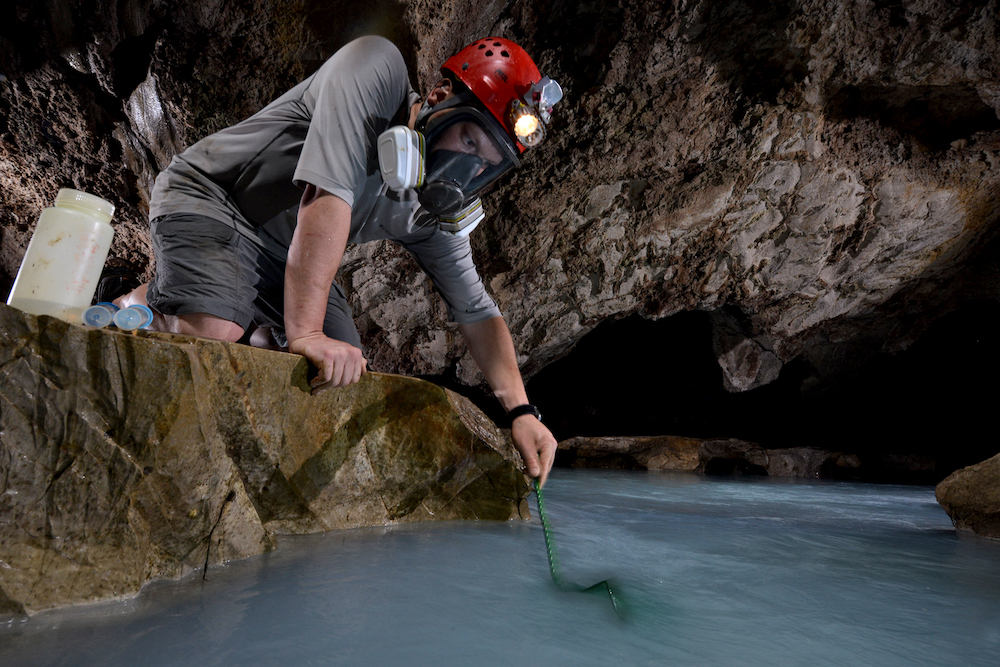
\includegraphics[width=1\linewidth]{images/field} \caption{That's right, I do real research, too... here collecting cave mollies in their natural habitat.}\label{fig:fieldwork}
\end{figure}

\hypertarget{the-cave-molly-and-its-ancestors}{%
\subsection{The Cave Molly and its Ancestors}\label{the-cave-molly-and-its-ancestors}}

The cave molly (\emph{Poecilia mexicana}) is a species of livebearing fish (family Poeciliidae) that occurs in two small caves in Southern Mexico (Parzefall 2001). One of the caves, the Cueva Luna Azufre, has a wetted area of only 39 square meters. Even though the available habitat is really small, there has been an isolated population of cave mollies in this cave for several thousand years. Interestingly, mollies also occur in adjacent surface habitats. The fish from the surface and cave habitats are clearly different phenotypically (Tobler et al.~2008; Figure \ref{fig:mollies}). The question is, what trait differences---if any---are a consequence of evolution? You will explore this question by visualizing several data sets, primarily comparing trait distributions across populations and generations.

\begin{figure}
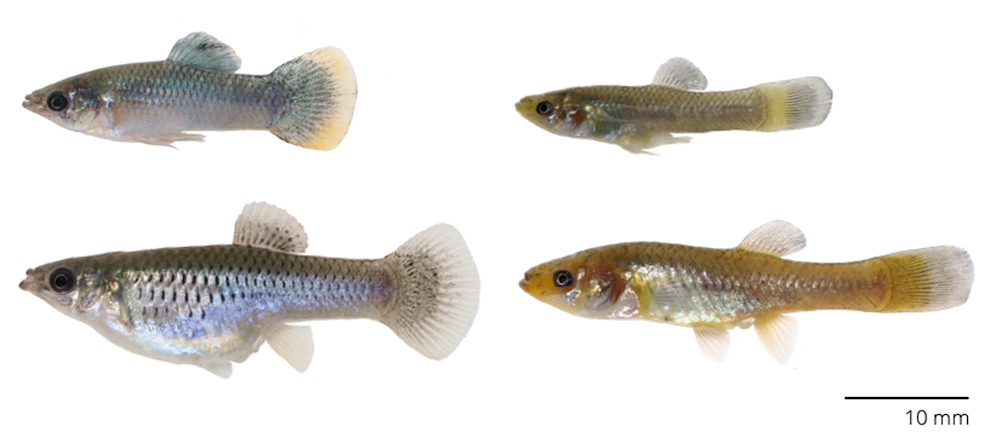
\includegraphics[width=1\linewidth]{images/mollies} \caption{Mollies occur in many surface streams throughout Mexico and Centeral America (left fish; male on top, female below). In the state of Tabasco, mollies have also colonized two caves, and fish from cave populations look noticeably different from their surface counterparts (right fish; male on top, female below). Photo: Michi Tobler}\label{fig:mollies}
\end{figure}

\hypertarget{practical-skills-number-sequences-allometry-and-histograms}{%
\section{Practical Skills: Number Sequences, Allometry, and Histograms}\label{practical-skills-number-sequences-allometry-and-histograms}}

\hypertarget{number-sequences}{%
\subsection{Number Sequences}\label{number-sequences}}

In \href{what-evolution-is.html\#some-r-and-rstudio-basics2}{chapter 1}, you learned how to make simple calculations with vectors; you will apply that skill in this exercise. In particular, you will calculate population sizes for multiple generations, which requires the creation of a vector with starting values (\emph{e.g.}, generations 1, 2, 3, etc.). You can create a vector (\texttt{x}) with a number sequence by using a colon with a number range. For example, \texttt{1:10} will generate a vector with numbers from 1 to 10.

\begin{Shaded}
\begin{Highlighting}[]
\CommentTok{\#Creating a vector x with a number sequence from 1{-}10}
\NormalTok{x }\OtherTok{\textless{}{-}} \DecValTok{1}\SpecialCharTok{:}\DecValTok{10}
\FunctionTok{print}\NormalTok{(x)}
\end{Highlighting}
\end{Shaded}

\begin{verbatim}
##  [1]  1  2  3  4  5  6  7  8  9 10
\end{verbatim}

As described before, you can then apply any function (\texttt{x\^{}2} in the example below) you want and store the output in a new vector (\texttt{y}, for example). Input and output variables can then be combined into the same data frame with the \texttt{data.frame()} and \texttt{cbind()} functions and ultimately plotted using \texttt{ggplot}:

\begin{Shaded}
\begin{Highlighting}[]
\CommentTok{\#Making some calculation based on x}
\NormalTok{y }\OtherTok{\textless{}{-}}\NormalTok{ x}\SpecialCharTok{\^{}}\DecValTok{2}
\FunctionTok{print}\NormalTok{(y)}
\end{Highlighting}
\end{Shaded}

\begin{verbatim}
##  [1]   1   4   9  16  25  36  49  64  81 100
\end{verbatim}

\begin{Shaded}
\begin{Highlighting}[]
\CommentTok{\#Combine the two vectors into a data frame}
\NormalTok{df }\OtherTok{\textless{}{-}} \FunctionTok{data.frame}\NormalTok{(}\FunctionTok{cbind}\NormalTok{(x,y))}
\FunctionTok{print}\NormalTok{(df)}
\end{Highlighting}
\end{Shaded}

\begin{verbatim}
##     x   y
## 1   1   1
## 2   2   4
## 3   3   9
## 4   4  16
## 5   5  25
## 6   6  36
## 7   7  49
## 8   8  64
## 9   9  81
## 10 10 100
\end{verbatim}

\begin{Shaded}
\begin{Highlighting}[]
\CommentTok{\#Plotting the results}
\FunctionTok{ggplot}\NormalTok{(df, }\FunctionTok{aes}\NormalTok{(}\AttributeTok{x=}\NormalTok{x, }\AttributeTok{y=}\NormalTok{y)) }\SpecialCharTok{+}
    \FunctionTok{geom\_point}\NormalTok{() }\SpecialCharTok{+}
    \FunctionTok{theme\_classic}\NormalTok{()}
\end{Highlighting}
\end{Shaded}

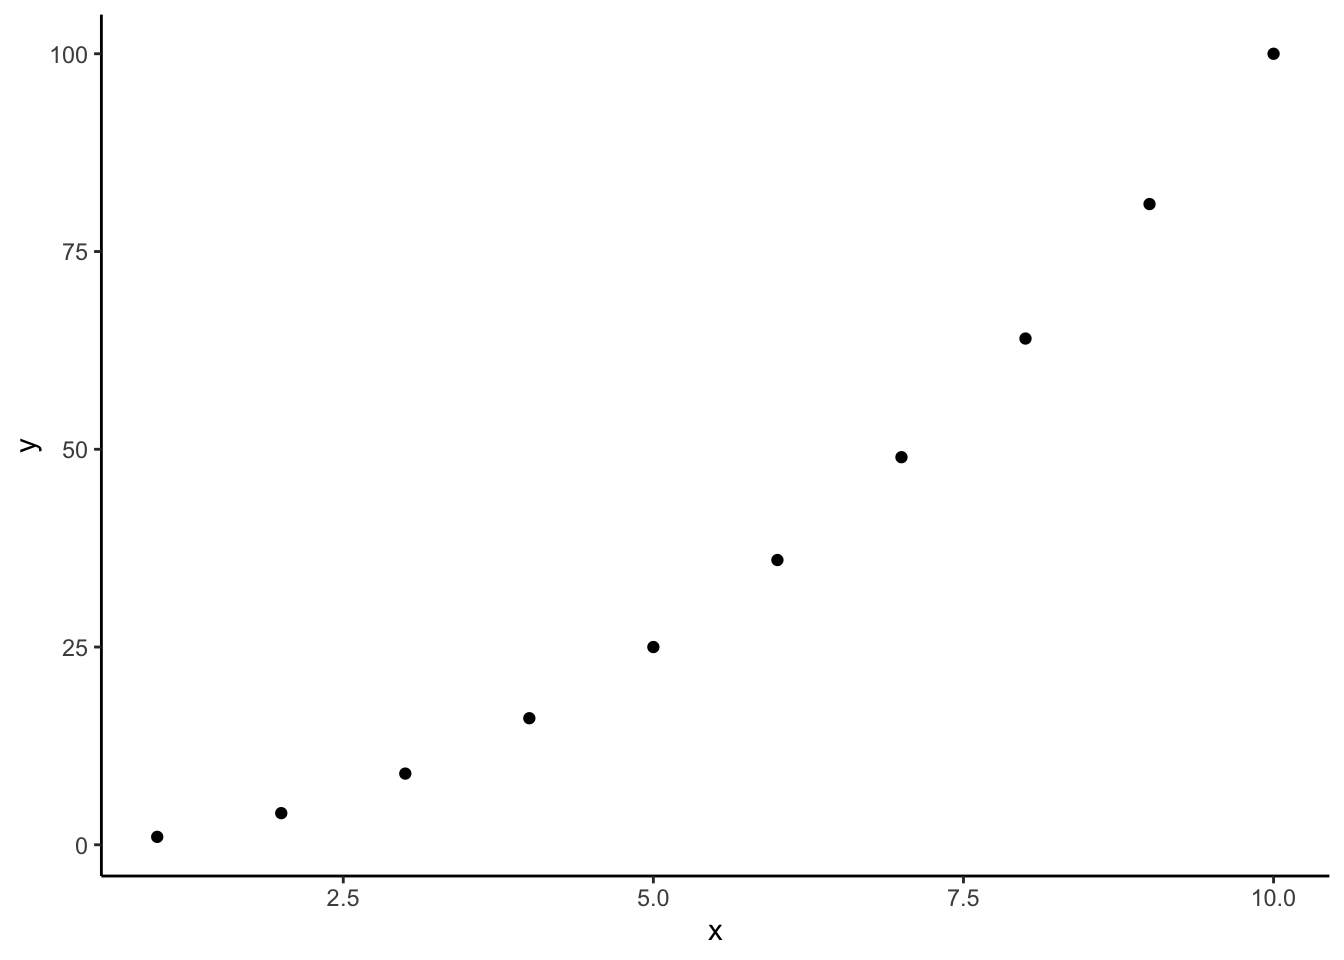
\includegraphics{Primer2Evolution_files/figure-latex/yx2-1.pdf}

\hypertarget{allometry-residuals}{%
\subsection{Allometry \& Residuals}\label{allometry-residuals}}

The data you will be looking at in this exercise comes from morphological measurements. Many traits, and morphological measurements in particular, are highly dependent on the body size of an individual. Think about it from a human perspective: larger individuals tend to have larger heads, longer legs, and longer arms. Despite this overall trend, the relative proportion of different body parts varies among individuals. Your roommate may be several inches shorter than you, but the two of you may still have the same shoe size; it's because relative to their height, they have large feet. More importantly, the relative proportions of different body parts changes predictably during development, a phenomenon we call allometry. Human babies are born with relatively large heads, and even though heads grow into adulthood, the rest of the body grows faster, thus changing the relative size of the head compared to the rest of the body.

How is this relevant to cave fish and evolution? Let's use a concrete \href{data/3_allometry.csv}{numerical example} to illustrate why taking allometric relationships into account is important for comparative analyses. Imagine we want to compare a particular trait (let's say head size) between two populations (A and B), and we predict one population would have larger heads. We could just measure head size, compare it between populations, and conclude that population A indeed has larger heads on average (Figure \ref{fig:headsize}).

\begin{Shaded}
\begin{Highlighting}[]
\NormalTok{allometry }\OtherTok{\textless{}{-}} \FunctionTok{read.csv}\NormalTok{(}\StringTok{"data/3\_allometry.csv"}\NormalTok{)}

\FunctionTok{ggplot}\NormalTok{(allometry, }\FunctionTok{aes}\NormalTok{(}\AttributeTok{x=}\NormalTok{population, }\AttributeTok{y=}\NormalTok{head.size)) }\SpecialCharTok{+}
    \FunctionTok{geom\_boxplot}\NormalTok{() }\SpecialCharTok{+}
    \FunctionTok{xlab}\NormalTok{(}\StringTok{"Population"}\NormalTok{) }\SpecialCharTok{+}
    \FunctionTok{ylab}\NormalTok{(}\StringTok{"Head size"}\NormalTok{) }\SpecialCharTok{+}
    \FunctionTok{theme\_classic}\NormalTok{()}
\end{Highlighting}
\end{Shaded}

\begin{figure}
\centering
\includegraphics{Primer2Evolution_files/figure-latex/headsize-1.pdf}
\caption{\label{fig:headsize}Head size differences between two hypothetical populations, A and B, illustrated with a \href{graph-library.html\#box-plot}{box plot}.}
\end{figure}

Case closed? Not so fast! It turns out that the two populations also differ in body size (Figure \ref{fig:bodysize}). This difference in body size could be real (individuals in population A are in fact larger) or just an artifact, because we happened to catch more large individuals in one of the populations (nonrandom sampling).

\begin{Shaded}
\begin{Highlighting}[]
\FunctionTok{ggplot}\NormalTok{(allometry, }\FunctionTok{aes}\NormalTok{(}\AttributeTok{x=}\NormalTok{population, }\AttributeTok{y=}\NormalTok{body.size)) }\SpecialCharTok{+}
    \FunctionTok{geom\_boxplot}\NormalTok{() }\SpecialCharTok{+}
    \FunctionTok{xlab}\NormalTok{(}\StringTok{"Population"}\NormalTok{) }\SpecialCharTok{+}
    \FunctionTok{ylab}\NormalTok{(}\StringTok{"Body size"}\NormalTok{) }\SpecialCharTok{+}
    \FunctionTok{theme\_classic}\NormalTok{()}
\end{Highlighting}
\end{Shaded}

\begin{figure}
\centering
\includegraphics{Primer2Evolution_files/figure-latex/bodysize-1.pdf}
\caption{\label{fig:bodysize}Body size differences between two hypothetical populations, A and B.}
\end{figure}

The congruence in head and body size differences raises the question whether population A just has larger heads because individuals in that population are larger. To investigate this, we can plot head size against body size---and lo and behold, there is a strong positive correlation between the two variables (Figure \ref{fig:allometry}). This is important if our prediction about the action of selection is specifically about head size and not body size. In that case, we want to know explicitly whether individuals in one population have a larger head relative to their body size compared to the other population. In other words, we want to know whether the residuals (\emph{i.e.}, the distance between a point and the best fit line, as indicated with blue segments in Figure \ref{fig:allometry}) are primarily positive for individuals coming from population A (indicating larger head size than expected for a given body size) and negative for individuals coming from population B (indicating smaller head size than expected for a given body size).

\begin{Shaded}
\begin{Highlighting}[]
\CommentTok{\#Calculating regression line}
\NormalTok{fit }\OtherTok{\textless{}{-}} \FunctionTok{lm}\NormalTok{(head.size }\SpecialCharTok{\textasciitilde{}}\NormalTok{ body.size, }\AttributeTok{data =}\NormalTok{ allometry)}
\CommentTok{\#Saving predicted values}
\NormalTok{allometry}\SpecialCharTok{$}\NormalTok{predicted }\OtherTok{\textless{}{-}} \FunctionTok{predict}\NormalTok{(fit)}

\FunctionTok{ggplot}\NormalTok{(allometry, }\FunctionTok{aes}\NormalTok{(}\AttributeTok{x=}\NormalTok{body.size, }\AttributeTok{y=}\NormalTok{head.size)) }\SpecialCharTok{+}
    \FunctionTok{geom\_segment}\NormalTok{(}\FunctionTok{aes}\NormalTok{(}\AttributeTok{xend =}\NormalTok{ body.size, }\AttributeTok{yend =}\NormalTok{ predicted), }\AttributeTok{color=}\StringTok{"blue"}\NormalTok{) }\SpecialCharTok{+}
    \FunctionTok{geom\_smooth}\NormalTok{(}\AttributeTok{method=}\StringTok{"lm"}\NormalTok{, }\AttributeTok{color=}\StringTok{"gray"}\NormalTok{, }\AttributeTok{se =} \ConstantTok{FALSE}\NormalTok{) }\SpecialCharTok{+}
    \FunctionTok{geom\_point}\NormalTok{(}\FunctionTok{aes}\NormalTok{(}\AttributeTok{color=}\NormalTok{population)) }\SpecialCharTok{+}
    \FunctionTok{xlab}\NormalTok{(}\StringTok{"Body size"}\NormalTok{) }\SpecialCharTok{+}
    \FunctionTok{ylab}\NormalTok{(}\StringTok{"Head size"}\NormalTok{) }\SpecialCharTok{+}
    \FunctionTok{theme\_classic}\NormalTok{() }\SpecialCharTok{+}
    \FunctionTok{scale\_color\_brewer}\NormalTok{(}\AttributeTok{palette =} \StringTok{"Set2"}\NormalTok{)}
\end{Highlighting}
\end{Shaded}

\begin{figure}
\centering
\includegraphics{Primer2Evolution_files/figure-latex/allometry-1.pdf}
\caption{\label{fig:allometry}Hypothetical relationship between body size and head size in populations A and B, showing a clear positive correlation. Residuals are indicated by the length of the blue segments. Residuals above the line are positive (larger than expected head size for a given body size), those below the line are negative (smaller than expected head size for a given body size).}
\end{figure}

To make proper inferences about head size, we consequently need to account for the fact that this trait covaries with body size. One way of doing that is to calculate residual head size, which is the length of the blue lines in Figure \ref{fig:allometry}. To obtain the residuals, we first need to calculate a regression line with \texttt{lm(y\ \textasciitilde{}\ x,\ df)}. In the code chuck above, this was done with head size and body size as variables, and the results of the regression were saved in an object called \texttt{fit}. To extract the residuals, we can now just create a new variable (\texttt{res.head.size}) in our \texttt{allometry} data frame and extract the residuals from the \texttt{fit} object using the \texttt{residuals()} function:

\begin{Shaded}
\begin{Highlighting}[]
\CommentTok{\#Extract residuals and create a new variable res.head.size in the allometry data frame}
\NormalTok{allometry}\SpecialCharTok{$}\NormalTok{res.head.size }\OtherTok{\textless{}{-}} \FunctionTok{residuals}\NormalTok{(fit)}
\end{Highlighting}
\end{Shaded}

If we plot our new variable (\texttt{res.head.size}) against body size, you can see that there is no correlation between the two (\emph{i.e.}, the regression line is perfectly flat; Figure \ref{fig:sizecorr}). Hence, we successfully corrected for the confounding effect of body size. Again, points that are above the best fit line (\emph{i.e.}, positive values) are individuals that have larger head sizes accounting for their body size, those below (negative values) have smaller head sizes. Points that are exactly on the line have an expected head size for their body size.

\begin{Shaded}
\begin{Highlighting}[]
\FunctionTok{ggplot}\NormalTok{(allometry, }\FunctionTok{aes}\NormalTok{(}\AttributeTok{x=}\NormalTok{body.size, }\AttributeTok{y=}\NormalTok{res.head.size, }\AttributeTok{color=}\NormalTok{population)) }\SpecialCharTok{+}
    \FunctionTok{geom\_smooth}\NormalTok{(}\AttributeTok{method=}\StringTok{"lm"}\NormalTok{, }\AttributeTok{color=}\StringTok{"gray"}\NormalTok{, }\AttributeTok{se =} \ConstantTok{FALSE}\NormalTok{) }\SpecialCharTok{+}
    \FunctionTok{geom\_point}\NormalTok{() }\SpecialCharTok{+}
    \FunctionTok{xlab}\NormalTok{(}\StringTok{"Body size"}\NormalTok{) }\SpecialCharTok{+}
    \FunctionTok{ylab}\NormalTok{(}\StringTok{"Residual head size"}\NormalTok{) }\SpecialCharTok{+}
    \FunctionTok{theme\_classic}\NormalTok{() }\SpecialCharTok{+}
    \FunctionTok{scale\_color\_brewer}\NormalTok{(}\AttributeTok{palette =} \StringTok{"Set2"}\NormalTok{)}
\end{Highlighting}
\end{Shaded}

\begin{figure}
\centering
\includegraphics{Primer2Evolution_files/figure-latex/sizecorr-1.pdf}
\caption{\label{fig:sizecorr}Relationship between body size and residual head size. There is no correlation between the two traits because we corrected for body size.}
\end{figure}

Finally, comparing the residual values of head size between populations reveals that there are no differences in this trait at all (Figure \ref{fig:schead}).

\begin{Shaded}
\begin{Highlighting}[]
\FunctionTok{ggplot}\NormalTok{(allometry, }\FunctionTok{aes}\NormalTok{(}\AttributeTok{x=}\NormalTok{population, }\AttributeTok{y=}\NormalTok{res.head.size)) }\SpecialCharTok{+}
    \FunctionTok{geom\_boxplot}\NormalTok{() }\SpecialCharTok{+}
    \FunctionTok{xlab}\NormalTok{(}\StringTok{"Population"}\NormalTok{) }\SpecialCharTok{+}
    \FunctionTok{ylab}\NormalTok{(}\StringTok{"Residual head size"}\NormalTok{) }\SpecialCharTok{+}
    \FunctionTok{theme\_classic}\NormalTok{()}
\end{Highlighting}
\end{Shaded}

\begin{figure}
\centering
\includegraphics{Primer2Evolution_files/figure-latex/schead-1.pdf}
\caption{\label{fig:schead}Plotting relative head size reveals no differences between the two populations.}
\end{figure}

This semester, we will emphasize being cognizant of potential confounding variables (like body size) and being able to account for them whenever possible (for example by calculating residuals). In the exercise associated with this chapter, you will practice using residuals to analyze morphological data.

\hypertarget{histograms-and-density-functions}{%
\subsection{Histograms and Density Functions}\label{histograms-and-density-functions}}

Frequency histograms are used to visualize the distribution of continuous variables. Histograms use bars to depict the frequency (on the y axis) of distinct ranges (bins) of a dependent variable (on x). You can use \texttt{geom\_histogram()} to make a frequency histogram with \texttt{ggplot}. Only an x-variable is needed within \texttt{aes()}. This example is based on a \href{data/test_data.csv}{test data set}.

\begin{Shaded}
\begin{Highlighting}[]
\NormalTok{test.data }\OtherTok{\textless{}{-}} \FunctionTok{read.csv}\NormalTok{(}\StringTok{"data/test\_data.csv"}\NormalTok{)}

\FunctionTok{ggplot}\NormalTok{(test.data, }\FunctionTok{aes}\NormalTok{(length)) }\SpecialCharTok{+}
    \FunctionTok{geom\_histogram}\NormalTok{() }\SpecialCharTok{+}
    \FunctionTok{xlab}\NormalTok{(}\StringTok{"Length [mm]"}\NormalTok{) }\SpecialCharTok{+}
    \FunctionTok{ylab}\NormalTok{(}\StringTok{"Frequency"}\NormalTok{) }\SpecialCharTok{+}
    \FunctionTok{theme\_classic}\NormalTok{()}
\end{Highlighting}
\end{Shaded}

\includegraphics{Primer2Evolution_files/figure-latex/histex-1.pdf}

Similar to how regressions provide a best-fit line through a cloud of points, density functions can be used to provide a statistical representation of a trait's distribution. Density plots represent smoothed versions of histograms and can be visualized using \texttt{geom\_density()}. Unlike histograms, which use counts as units on the y-axis, density plots use relative frequency (number of observations in a bin divided by the total number of observations). To avoid issues with scale, you have to modify the aesthetics of \texttt{geom\_histogram()} with \texttt{aes(y=..density..)} when you combine the two graphical elements:

\begin{Shaded}
\begin{Highlighting}[]
\FunctionTok{ggplot}\NormalTok{(test.data, }\FunctionTok{aes}\NormalTok{(length)) }\SpecialCharTok{+}
    \FunctionTok{geom\_histogram}\NormalTok{(}\FunctionTok{aes}\NormalTok{(}\AttributeTok{y=}\NormalTok{..density..)) }\SpecialCharTok{+}
    \FunctionTok{geom\_density}\NormalTok{() }\SpecialCharTok{+}
    \FunctionTok{xlab}\NormalTok{(}\StringTok{"Length [mm]"}\NormalTok{) }\SpecialCharTok{+}
    \FunctionTok{ylab}\NormalTok{(}\StringTok{"Frequency"}\NormalTok{) }\SpecialCharTok{+}
    \FunctionTok{theme\_classic}\NormalTok{()}
\end{Highlighting}
\end{Shaded}

\includegraphics{Primer2Evolution_files/figure-latex/histdensex-1.pdf}

Finally, you can define subgroups in histograms and density plots to directly contrast patterns of variation between groups (rather than making separate plots). You can do this by adding \texttt{fill=variable} (for area colors) or \texttt{color=variable} (for edges and lines) to \texttt{aes()}, as illustrated with the variable \texttt{sex} below:

\begin{Shaded}
\begin{Highlighting}[]
\FunctionTok{ggplot}\NormalTok{(test.data, }\FunctionTok{aes}\NormalTok{(length, }\AttributeTok{fill=}\NormalTok{sex)) }\SpecialCharTok{+}
    \FunctionTok{geom\_histogram}\NormalTok{(}\FunctionTok{aes}\NormalTok{(}\AttributeTok{y=}\NormalTok{..density..)) }\SpecialCharTok{+}
    \FunctionTok{geom\_density}\NormalTok{(}\AttributeTok{alpha=}\NormalTok{.}\DecValTok{5}\NormalTok{) }\SpecialCharTok{+} \CommentTok{\#The alpha determines the degree of transparency}
    \FunctionTok{xlab}\NormalTok{(}\StringTok{"Length [mm]"}\NormalTok{) }\SpecialCharTok{+}
    \FunctionTok{ylab}\NormalTok{(}\StringTok{"Frequency"}\NormalTok{) }\SpecialCharTok{+}
    \FunctionTok{theme\_classic}\NormalTok{() }\SpecialCharTok{+}
    \FunctionTok{scale\_fill\_brewer}\NormalTok{(}\AttributeTok{palette =} \StringTok{"Set2"}\NormalTok{) }\CommentTok{\#This changes the color scheme to a colorblind{-}friendly palette (see Chapter 2)}
\end{Highlighting}
\end{Shaded}

\includegraphics{Primer2Evolution_files/figure-latex/histdensexex-1.pdf}

\hypertarget{reflection-questions-2}{%
\section{Reflection Questions}\label{reflection-questions-2}}

\begin{enumerate}
\def\labelenumi{\arabic{enumi}.}
\item
  In your own words, how do you define fitness? How would you measure fitness in a natural population? Provide a concrete example; \emph{i.e.}, be specific with what organism you have in mind and describe the concrete steps you would take to quantify fitness.
\item
  Think about the relation between natural selection and evolution. Can you explain why the presence of natural selection does not necessarily lead to evolutionary change? Can you explain how evolution might happen in the absence of natural selection?
\item
  If you look at the time series of beak size data from the Grants (Figure \ref{fig:timeseries}), you can see that after a steep increase in beak size right after the drought, beak sizes slowly decline throughout the 1980s. In fact, beak sizes reach pre-drought levels by the late 1980s. What do you think happened after the drought? Why did beak sizes not continue to increase or remain stable at a larger size?
\item
  In The Origin of Species, Darwin said:

  \begin{quote}
  ``As natural selection works solely by and for the good of each being, all corporeal and mental endowments will tend to progress toward perfection.''

  Darwin, 1859
  \end{quote}

  What do you think of this statement? Can you think of reasons why natural selection does not actually lead to perfection?
\end{enumerate}

\hypertarget{references-3}{%
\section{References}\label{references-3}}

\begin{itemize}
\tightlist
\item
  Boag, PT (1983). \href{https://onlinelibrary.wiley.com/doi/10.1111/j.1558-5646.1983.tb05618.x}{The heritability of external morphology in Darwin's ground finches (\emph{Geospiza}) on Isla Daphne Major, Galapagos}. \emph{Evolution} 37, 877--894.
\item
  Boag, PT, PR Grant (1981). \href{https://science.sciencemag.org/content/214/4516/82}{Intense natural selection in a population of Darwin's finches (Geospizinae) in the Galapagos}. \emph{Science} 214, 82--85.
\item
  Boag, PT, PR Grant (1984). \href{https://academic.oup.com/biolinnean/article-abstract/22/3/243/2666306}{The classical case of character release: Darwin's finches (\emph{Geospiza}) on Isla Daphne Major, Galápagos}. \emph{Biological Journal of the Linnean Society} 22 243--287.
\item
  Darwin, C. (1859). \emph{On the origin of species based on natural selection, or the preservation of favoured races in the struggle of life}. John Murray.
\item
  Dugatkin, LA (2018). \href{https://evolution-outreach.biomedcentral.com/articles/10.1186/s12052-018-0090-x}{The silver fox domestication experiment}. \emph{Evolution: Education and Outreach} 11, 1--5.
\item
  Grant, PR, BR Grant (2002). \href{https://science.sciencemag.org/content/296/5568/707}{Unpredictable evolution in a 30-year study of Darwin's finches}. \emph{Science} 296: 707-711.
\item
  Grant, RB, PR Grant (2003). \href{https://academic.oup.com/bioscience/article/53/10/965/254944}{What Darwin's Finches can teach us about the evolutionary origin and regulation of biodiversity}. \emph{Bioscience} 53, 965--975.
\item
  Parzefall, J (2001). \href{https://link.springer.com/article/10.1023/A:1011899817764}{A review of morphological and behavioural changes in the cave molly, \emph{Poecilia mexicana}, from Tabasco, Mexico}. \emph{Environmental Biology of Fishes} 62, 263--275.
\item
  Tobler, M, TJ Dewitt, I Schlupp, FJ García de León, R Herrmann, PGD Feulner, \ldots{} M Plath (2008). \href{https://onlinelibrary.wiley.com/doi/full/10.1111/j.1558-5646.2008.00466.x}{Toxic hydrogen sulfide and dark caves: phenotypic and genetic divergence across two abiotic environmental gradients in \emph{Poecilia mexicana}}. \emph{Evolution} 62, 2643--2659.
\end{itemize}

\hypertarget{part-a-genetic-perspective-on-evolution}{%
\part{A Genetic Perspective on Evolution}\label{part-a-genetic-perspective-on-evolution}}

\hypertarget{the-raw-materials-for-evolution}{%
\chapter{The Raw Materials for Evolution}\label{the-raw-materials-for-evolution}}

So far, we have primarily explored the process of evolution from a phenotypic perspective. We considered how ecological sources of selection impact the survival and reproduction of individuals expressing different heritable traits, and how fitness differences of variants in turn impact the phenotypic composition of subsequent generations. While there is nothing inherently wrong with this approach, it ignores the mechanisms that underlie the expression of phenotypic traits and inheritance. Darwin was also agnostic about these aspects, largely treating what we call ``genetics'' as a black box. He was unaware of the work of his contemporary, Gregor Mendel, an Augustinian friar that established some of the basic tenets of heredity. It was not until the 1930s and 1940s that genetics and Darwinian evolution were integrated into a unified theory. The fusion of the two fields is known as the Modern Synthesis.

A number of biologists made critical contributions to the Modern Synthesis. Ronald Fisher, Jack Haldane, and Sewall Wright are credited with developing the theoretical basis of population genetics. Theodosius Dobzhansky pioneered evolutionary genetic studies in natural populations, chiefly using \emph{Drosophila} fruit flies to provide empirical evidence that supported the theoretical developments. Ernst Mayr shaped the modern definition of species and framed critical hypotheses about how speciation occurs. And finally, George Gaylord Simpson integrated findings from paleontology with those in genetics and natural selection.

The Modern Synthesis largely strengthened Darwin's notion of evolution by closing critical gaps associated with the mechanisms of heredity. This allowed for a more complete and nuanced understanding of evolutionary processes. Rather than just investigating how selection shapes phenotypic variation, a modern view of evolution takes into account how genes and the environment interact to shape developmental and physiological processes that give rise to phenotypic traits of functioning organisms (Figure \ref{fig:beyondphenotype}). The environment also tests phenotypic variants, causing fitness differences that ultimately change the genetic composition of subsequent generations (Figure \ref{fig:beyondphenotype}). In the following chapters, we will explore the genetic basis of evolutionary change and discuss how the many facets of ecology shape trait expression and evolution.

\begin{figure}
\includegraphics[width=1\linewidth]{images/g2p2} \caption{Conceptual framework of a modern perspective on evolution that includes the genetic basis of phenotypic traits.}\label{fig:beyondphenotype}
\end{figure}

The first task in exploring evolution from a genetic perspective is to establish how genomic variation translates to phenotypic variation. We will then discuss the fundamental sources of genetic variation, how we can quantify such variation in natural populations, and how we can use knowledge of genetic variation to test simple evolutionary hypotheses.

\hypertarget{the-genotype-phenotype-gap}{%
\section{The Genotype-Phenotype Gap}\label{the-genotype-phenotype-gap}}

A common misconception about the origin of novel phenotypic variants is that they are primarily caused by mutations in protein-coding regions of the genome, which change the structure and function of a protein and ultimately create variation in a particular trait. In reality, the ways by which genetic variation can impact phenotypic traits are much more diverse and complex. While technological breakthroughs over the past decades have made it relatively easy to quantify genetic variation across the genome (see below), connecting mutations at particular loci to phenotypic traits has proven much more challenging. We call this the genotype-phenotype gap, and closing this gap is one of the biggest challenges in modern biology.

Part of the complexity arises from the sheer number of genes in a genome. The human genome, for example, consists of over 30,000 genes. More importantly, one-to-one mapping---where one gene causes the expression of a specific phenotypic trait or at least an aspect of it---is relatively rare; rather, genes and their derivative products (different RNAs, proteins, and ultimately metabolites) interact in complex ways, such that the mapping is really many-to-many (many genes affect multiple traits at ones). These complexities become evident when we consider a simple genotype-phenotype framework, such as illustrated in Figure \ref{fig:g2p}.

\begin{figure}
\includegraphics[width=1\linewidth]{images/g2p} \caption{Emergent phenotypic traits are the product of variation in the genome and the environmentally-dependent expression of that genomic variation. Figure adopted from Ritchie et al. (2005). Beetle photo by [Udo Schmidt](https://www.flickr.com/photos/coleoptera-us/), [CC BY-SA 2.0](https://creativecommons.org/licenses/by-sa/2.0/).}\label{fig:g2p}
\end{figure}

RNA is transcribed from DNA by RNA polymerase, which produces messenger RNAs (mRNAs) that serve as templates for protein synthesis. After transcription, introns are removed by RNA splicing, and alternative splicing can recombine different exons from the same gene, which allows a single gene to code for multiple proteins with different functions. In addition, not all RNAs transcribed from DNA lead to functional proteins. Micro RNAs (miRNA) are short, non-coding RNA molecules that can silence mRNAs, and thus play a role in the post-transcriptional regulation of gene expression. Essentially, miRNAs bind to mRNAs with complementary sequences, which causes those mRNAs to degrade and interrupts the translation of mRNAs into functional proteins. In summary, RNAs play a critical role in multiple processes, not only because they encode templates for protein synthesis, but also because they can regulate the amount of protein produced by other genes.

Similar complexities are also evident at the proteome level. Sometimes, a single type of mRNA gives rise to a functional protein after translation. But many enzymes are actually multi-protein complexes and require information from multiple genes to make one functional unit. A great example are the enzymes associated with the oxidative phosphorylation (OxPhos) pathway in mitochondria, which produce the majority of the ATP needed for maintenance of cellular function. All five OxPhos enzymes are multi-protein complexes, and complex I (NADH dehydrogenase) is composed of 45 subunits, not counting the proteins involved in the assembly of the enzyme. Furthermore, some proteins actually act as transcription factors (TF in Figure \ref{fig:g2p}). These transcription factors bind to transcription factor binding sites (TFbs) in the genome, either enhancing or suppressing the expression of other genes. So proteins are also involved in complex feedback loops that regulate gene expression in response to various internal and external stimuli.

Finally, different enzymes are organized into interconnected pathways that process the metabolites required for the maintenance of organismal function. Figure \ref{fig:metabolism} provides a glimpse at some of the metabolic pathways in human cells. As you can imagine, these metabolic networks are full of redundancy, such that similar phenotypic outcomes may actually be caused by different underlying mechanisms.

\begin{figure}
\includegraphics[width=1\linewidth]{images/metabolic_pathway} \caption{Pathway map representing the molecular interaction, reaction, and relation networks for human metabolism. Check out the [KEGG Pathway Database](https://www.genome.jp/pathway/hsa01100) for an interactive version.}\label{fig:metabolism}
\end{figure}

It is the action and interaction of biological processes across all of these levels of organismal organization that ultimately shape the phenotypic traits frequently studied by evolutionary biologists. As you can imagine, reconciling evolutionary patterns across these levels is not always trivial, simply because we don't always know what genes are connected to what traits. In addition, even superficial examination of genotype-phenotype relationships shows that variation in phenotypes can not only arise from variation in protein structure and function, but also differences in when, where, and at what levels proteins are expressed. Phenotypic variants may arise as a consequence of changes in the amino acid sequences of proteins, or changes in the regulation of protein expression. In that light, let's investigate how different mutations arise in the genome, how they might impact organismal phenotypes, and what their potential evolutionary ramifications are.

Explore More

If you are interested in learning more about what changes in DNA are responsible for the evolution of phenotypic diversity, check out this short essay by Sean Carroll: \href{https://www.cell.com/cell/fulltext/S0092-8674(00)80868-5}{\emph{The Evolution of Gene Regulation and Morphological Diversity}}. I also recommend his popular science book \href{https://www.amazon.com/Endless-Forms-Most-Beautiful-Science/dp/0393327795}{\emph{Endless Forms Most Beautiful: The New Science of Evo-Devo}}.

\hypertarget{mutation-the-fundamental-source-of-novelty}{%
\section{Mutation: The Fundamental Source of Novelty}\label{mutation-the-fundamental-source-of-novelty}}

Mutation is the fundamental source of variation that selection can act upon to create evolutionary change. Any change in the nucleotide sequence of a genome is considered a mutation. Mutations can involve single nucleotide substitutions, insertions and deletions (also called indels), inversions of chromosome segments, duplication of chromosome segments, and partial and complete genome duplications. Different types of mutations have different molecular origins and different consequences for the expression of phenotypic traits. Consequently, they also have different evolutionary implications.

Definition: Mutation

A mutation is a change in DNA sequence, resulting in a variant form (allele) that can be passed on to subsequent generations.

\hypertarget{point-mutations}{%
\subsection{Point Mutations}\label{point-mutations}}

Point mutations are changes in a single nucleotide of DNA. They include transitions and transversions that cause single nucleotide substitutions as well as single nucleotide insertions and deletions. Point mutations cause single nucleotide polymorphisms (SNPs; single base-pair differences in the DNA sequence), which are the basis for many population genetic analyses.

\hypertarget{origins}{%
\subsubsection*{Origins}\label{origins}}
\addcontentsline{toc}{subsubsection}{Origins}

Point mutations primarily arise from mistakes during DNA replication. The mutations are either caused by random errors made by DNA polymerase (which copies the DNA during replication) or by random errors made by enzymes involved in DNA repair.

\hypertarget{phenotypic-impact-and-evolutionary-consequences}{%
\subsubsection*{Phenotypic Impact and Evolutionary Consequences}\label{phenotypic-impact-and-evolutionary-consequences}}
\addcontentsline{toc}{subsubsection}{Phenotypic Impact and Evolutionary Consequences}

The phenotypic impacts and evolutionary consequences of point mutations depend on the location and nature of the mutation.

In protein-coding regions of the genome, single nucleotide substitutions can either be synonymous (silent) or nonsynonymous. Synonymous mutations arise due to redundancy of the genetic code, where multiple nucleotide triplets encode for the same amino acid (Figure \ref{fig:geneticcode}). For example, a mutation from AGG to AGA has no effect on the resulting amino acid sequence, because both triplets encode for arginine. Since such synonymous mutations do not translate to changes in the resulting protein, there are no consequences for expressed phenotypes and the mutation is not visible to selection (\emph{i.e.}, it has no fitness consequences).

\begin{figure}
\includegraphics[width=1\linewidth]{images/genetic_code} \caption{Diagram of the genetic code showing which DNA bases code for which amino acids (in different colors).}\label{fig:geneticcode}
\end{figure}

In contrast, nonsynonymous substitutions do change the amino acid sequence of the resulting protein (\emph{e.g.}, AGG to AGT changes arginine to serine; \ref{fig:geneticcode}). Amino acid substitutions can fundamentally change the structure and function of proteins, with corresponding consequences for downstream phenotypes. There are three potential evolutionary consequences of nonsynonymous substitutions: (i) the altered protein and resulting phenotypic changes are deleterious, imposing a fitness disadvantage for the individual; (ii) the altered protein and resulting phenotypic changes are beneficial, providing a fitness advantage for the individual; or (iii) the altered protein does not change its structure and function in a significant way, in which case even a nonsynonymous mutation can be selectively neutral.

Protein-coding regions of the genome can also be impacted by indels. Single nucleotide indels are known as frameshift mutations, because they alter the reading frame at which nucleotide triplets are translated into amino acids. Consequently, an insertion or a deletion of a single nucleotide can completely change the amino acid sequence of the resulting protein or introduce a premature stop codon (Figure \ref{fig:frameshift}). Many frameshift mutations cause loss of function in a protein and consequently lead to fitness reductions in individuals carrying the mutation.

\begin{figure}
\includegraphics[width=1\linewidth]{images/insertion} \caption{Frameshift mutations caused by insertions or deletions change the amino acid sequence and potentially insert premature stop codons.}\label{fig:frameshift}
\end{figure}

Protein-coding regions only make up about 1 \% of the human genome (and even less in some other organisms). Point mutations can also occur in non-coding genomic regions. Some non-coding regions serve important functions in gene regulation (\emph{e.g.}, transcription factor binding sites, non-coding RNAs) or in mRNA processing and protein translation (\emph{e.g.}, introns). Hence, point mutations in such genomic regions may still impact organismal phenotypes, and---depending on the context---they can come with fitness costs or benefits.

Finally, putatively non-functional genomic regions (pseudogenes and repeat sequences caused by transposons and retrotransposons) can make up large portions of a genome. Point mutations in these genomic regions largely have no fitness consequences; hence, they tend to be selectively neutral.

\hypertarget{inversions}{%
\subsection{Inversions}\label{inversions}}

Inversions are regions of chromosomes that are flipped in direction. These mutations do not change the amount or kind of genetic material in the genome, only its sequential arrangement (Figure \ref{fig:inversion}).

\begin{figure}
\includegraphics[width=1\linewidth]{images/inversion} \caption{Inversions are caused when double breaks in the DNA (indicated by asterisks) are fixed upon a central element flipping in direction.}\label{fig:inversion}
\end{figure}

\hypertarget{origins-1}{%
\subsubsection*{Origins}\label{origins-1}}
\addcontentsline{toc}{subsubsection}{Origins}

Inversions are caused by double DNA breaks, in which the broken central piece is flipped before the DNA strands are joined back together by DNA ligase. While inversions can be only a few base pairs long (in which case they can act like point mutations), some are very large (\textgreater4 megabases) and contain multiple functional genes.

\hypertarget{phenotypic-impact-and-evolutionary-consequences-1}{%
\subsubsection*{Phenotypic Impact and Evolutionary Consequences}\label{phenotypic-impact-and-evolutionary-consequences-1}}
\addcontentsline{toc}{subsubsection}{Phenotypic Impact and Evolutionary Consequences}

If the break points are located within a functional gene, inversions can cause the loss of function and corresponding negative impacts on phenotypic expression and fitness. In most cases, however, break points are located in intergenic regions, such that inversions have no visible phenotypic repercussions. Nonetheless, inversions can play an important role in evolution, especially if they contain multiple functional genes. In heterozygous individuals that have one copy of the chromosome with and one without the inversion, the likelihood of recombination within the inversion is reduced because of mechanical pairing issues associated with non-complimentary DNA. As a result, genes within an inversion are often inherited in blocks and have a reduced chance to be reshuffled during sex and recombination.

\hypertarget{gene-duplication}{%
\subsection{Gene Duplication}\label{gene-duplication}}

Gene duplication occurs when entire segments of a chromosome containing functional genes are duplicated, creating novel copies in the genome.

\hypertarget{origins-2}{%
\subsubsection*{Origins}\label{origins-2}}
\addcontentsline{toc}{subsubsection}{Origins}

Most gene duplications arise from unequal crossing-overs during meiosis, where misalignment of homologous chromosomes leads to daughter chromosomes of different lengths. One daughter chromosome contains a duplicated segment that is missing from the other (Figure \ref{fig:uneqcross}). Gene duplications can also be associated with replication slippage and retrotransposon activity.

\begin{figure}
\includegraphics[width=1\linewidth]{images/duplication} \caption{Crossing-over between misaligned chromosomes during meiosis (A) causes DNA segments to be deleted in one and inserted in the other chromosome (B).}\label{fig:uneqcross}
\end{figure}

\hypertarget{phenotypic-impact-and-evolutionary-consequences-2}{%
\subsubsection*{Phenotypic Impact and Evolutionary Consequences}\label{phenotypic-impact-and-evolutionary-consequences-2}}
\addcontentsline{toc}{subsubsection}{Phenotypic Impact and Evolutionary Consequences}

Individuals that inherit a chromosome with a deleted essential gene may suffer from negative phenotypic and fitness effects. Those that inherit a chromosome with a duplication, however, are unlikely to suffer from adverse consequences. There are two possible evolutionary consequences for the genes within a duplication. First, a duplicated gene may accumulate a variety of mutations, even deleterious ones. But since a functional copy is still present in the genome, individual carriers will not face any fitness reductions. As deleterious mutations accumulate in the duplicated gene, it will eventually become a non-functional pseudogene. These pseudogenes are passed on across generations, as discussed in \href{evidence-for-evolution.html}{Chapter 2}. Alternatively, a duplicated gene may accumulate mutations that change the structure and function of the resulting protein in a beneficial way, enhancing the fitness of the carrier. As such, gene duplication can be a major source of genomic novelty, and many gene families have arisen through duplication.

Hemoglobin genes, for example, have duplicated repeatedly during vertebrate evolution. Different hemoglobin genes in the human genome vary in their functional properties and expression depending on developmental stage or environmental conditions. Hemoglobins expressed during fetal development have a higher oxygen affinity than the mother's hemoglobin, allowing the fetus to extract oxygen from the mother's blood. Similarly, our bodies express different types of hemoglobins during acclimation to low oxygen concentrations at high altitudes. Shifting to the expression of alternative hemoglobins takes time, which explains why you may experience altitude sickness on the first days of your Colorado vacation. Once you are acclimated, the higher oxygen binding capacity of alternative hemoglobins allows you to perform normally even at higher altitudes, which is why some athletes use high-elevation training to gain an advantage for competitions close to sea level. Consequently, gene duplication is an important source of novelty in the genome and allows for the evolution of specialized functions that are constrained by the number of loci.

\hypertarget{genome-duplication}{%
\subsection{Genome Duplication}\label{genome-duplication}}

Genome duplications occur when additional copies of the entire genome are generated, leading to polyploidy. In some instances, genome duplications can be partial, if only a subset of chromosomes are duplicated.

\hypertarget{origins-3}{%
\subsubsection*{Origins}\label{origins-3}}
\addcontentsline{toc}{subsubsection}{Origins}

Partial and complete genome duplications occur because of segregation errors during meiosis. Non-disjunction during the anaphase of meiosis I or II leads to a failure of correct chromosome separation into daughter cells, resulting in gametes with extra or missing chromosomes.

\begin{figure}
\includegraphics[width=1\linewidth]{images/nondisjunction} \caption{Metaphase: Chromosomes line up in the middle plane, the meiotic spindle forms, and the kinetochores (black) of sister chromatids attach to the microtubules (blue lines). Anaphase: Sister chromatids separate and the microtubules pull them in opposite directions. The chromosome shown in purple fails to separate properly, with its sister chromatids sticking together and getting pulled to the same side. This results in nondisjunction of the chromosome.}\label{fig:nondisjunction}
\end{figure}

\hypertarget{phenotypic-impact-and-evolutionary-consequences-3}{%
\subsubsection*{Phenotypic Impact and Evolutionary Consequences}\label{phenotypic-impact-and-evolutionary-consequences-3}}
\addcontentsline{toc}{subsubsection}{Phenotypic Impact and Evolutionary Consequences}

Whole genome duplications do not typically have immediate negative consequences for the carrier. Like gene duplication, it may actually allow for the evolution of novel genes, because they release constraints associated with pleiotropic effects. However, polyploids are instantaneously reproductively isolated from their ancestors, because proper meiosis is not possible with an uneven number of sister chromosomes. Hence, we see polyploid lineages more commonly in organisms with asexual reproduction or self-fertilization, like plants. In these cases, polyploidization is associated with instantaneous speciation.

In contrast, partial genome duplications often have negative fitness consequences for the carrier. This is thought to be related to gene dosage effects, where the amount of gene product (\emph{e.g.}, protein) is correlated with the number of copies of a particular gene in the genome. Hence, partial genome duplication can lead to biases in the expression of some---but not all---genes, creating imbalances in the developmental and metabolic networks that have been fine-tuned by evolution.

\hypertarget{mutation-rates}{%
\section{Mutation Rates}\label{mutation-rates}}

Point mutations are by far the most common mutations in the genome. Estimation of mutation rates is not trivial, and estimates vary depending on how these rates are actually quantified. The earliest estimates came from experimental mutation accumulation lines, where mutation rates were estimated based on visible phenotypic mutations that were likely caused by loss of function mutations (\emph{e.g.}, premature stop-codons, frame-shift mutations, etc.). These experiments estimated mutations rates per genome per generation, and revealed values between 0.0025 in \emph{E. coli} and 1.6 in humans (Table 4.1).

The 640-fold variation in the organisms listed in Table 4.1 is primarily caused by two factors. Per-genome mutation rates roughly scale with genome size; larger genomes tend to have have a higher likelihood of accruing copy errors. More importantly, however, mutation rates are higher in multicellular organisms. In unicellular organisms, every round of DNA replication represents a new generation. In contrast, mutations also occur during mitosis as multicellular bodies develop. Any mutation within the germ line will be passed on to the next generation.

\begin{longtable}[]{@{}
  >{\raggedright\arraybackslash}p{(\columnwidth - 2\tabcolsep) * \real{0.4267}}
  >{\raggedleft\arraybackslash}p{(\columnwidth - 2\tabcolsep) * \real{0.5733}}@{}}
\caption{Table 4.1: Mutation rates for different taxa.}\tabularnewline
\toprule
\begin{minipage}[b]{\linewidth}\raggedright
Taxon
\end{minipage} & \begin{minipage}[b]{\linewidth}\raggedleft
Mutation rate (per genome per generation)
\end{minipage} \\
\midrule
\endfirsthead
\toprule
\begin{minipage}[b]{\linewidth}\raggedright
Taxon
\end{minipage} & \begin{minipage}[b]{\linewidth}\raggedleft
Mutation rate (per genome per generation)
\end{minipage} \\
\midrule
\endhead
\emph{Escherichia coli} & 0.0025 \\
\emph{Saccharomyces acidocaldarius} & 0.0018 \\
\emph{Saccharomyces cerevisiae} & 0.0027 \\
\emph{Caenorhabditis elegans} & 0.0360 \\
\emph{Mus musculus} & 0.9000 \\
\emph{Homo sapiens} & 1.6000 \\
\bottomrule
\end{longtable}

While these mutation rates seem small, it is important to remember that a population typically consists of many genomes (\emph{i.e.}, individuals). For example, an industrial batch of beer is estimated to harbor about 100 billion (10\textsuperscript{11}) yeast cells. Given a mutation rate of 0.0027 (Table 4.1), that includes 270 million (2.7*10\textsuperscript{8}) mutations. Considering that yeast has a genome size of about 12 Mb (1.2*10\textsuperscript{7} base pairs), that means that every nucleotide in the genome might mutate up to 20 times in every generation. You can conduct the same calculation with humans (population size: 7.9 billion; genome size: 3.2*10\textsuperscript{9} base pairs), and you will find that every nucleotide may mutate about twice in each generation. So while the likelihood for a particular mutation to occur in an individual is very small, the mutational input---especially in large populations---can be considerable.

More importantly, mutation rate estimates based on mutation accumulation experiments vastly underestimate actual mutation rates. As discussed above, many mutations have no or only minute phenotypic effects, and are thus impossible to detect during phenotype screens. Unsurprisingly, mutation rate estimates based on DNA sequencing have revealed much higher mutation rates. For example, the rate of nucleotide substitutions in humans is estimated at about 1 in 10\textsuperscript{8} in every generation. Extrapolated for the size of the human genome, this means that every gamete produced exhibits about 30 mutations.

\hypertarget{quantifying-genetic-variation}{%
\section{Quantifying Genetic Variation}\label{quantifying-genetic-variation}}

As mutation continuously introduces new genetic variation into a population's gene pool, biologists want to quantify the distribution and changes in genetic variation across generations. With the massive improvements of DNA sequencing technologies over the past two decades, we can now directly sequence partial or whole genomes to detect single nucleotide polymorphisms (SNPs; Figure \ref{fig:snps}) that are the consequence of point mutations.

\begin{figure}
\includegraphics[width=1\linewidth]{images/SNP} \caption{A Single Nucleotide Polymorphism (SNP) is a change of nucleotides at a single base-pair location on DNA.}\label{fig:snps}
\end{figure}

Explore More

If you are interested in learning more about modern DNA sequencing technologies, check out the review paper by Sara Goodwin and colleagues: \href{https://www-nature-com.er.lib.k-state.edu/articles/nrg.2016.49}{\emph{Coming of age: ten years of next-generation sequencing technologies}}.

For population genetic analyses, researchers typically sample dozens to hundreds of individuals from one or many populations for genotyping by sequencing. Based on the sequencing data, we can then determine the genotype of each individual. Assuming a bi-allelic locus, there are three possible genotypes: \emph{AA}, \emph{Aa}, and \emph{aa}. At a population level, we can then describe genetic variation with two metrics: the relative genotype frequency and the relative allele frequency.

The relative genotype frequency is the proportion of individuals with a particular genotype, showing the distribution of genetic variation in a population. The sum of genotype frequencies (\emph{f}) equals one, as shown here for a bi-allelic locus:

\begin{equation} 
f_{AA}+f_{Aa}+f_{aa}=1 \label{eq:1} 
\end{equation}

The relative allele frequency is the proportion of different alleles at a particular locus and measures the amount of genetic variation in a population. Allele frequencies can be calculated based on the relative genotype frequencies measured by sequencing. For a bi-allelic locus in a diploid organism, the frequencies of \emph{A} (\emph{p}) and \emph{a} (\emph{q}) can be calculated as follows:

\begin{align}
f_A=p=\frac{2f_{AA}+f_{Aa}}{2(f_{AA}+f_{Aa}+f_{aa})}=f_{AA}+0.5*f_{Aa} \label{eq:2} \\
f_a=q=\frac{2f_{aa}+f_{Aa}}{2(f_{AA}+f_{Aa}+f_{aa})}=f_{aa}+0.5*f_{Aa} \label{eq:3} 
\end{align}

Remember, if Equation \eqref{eq:1} is true, then the sum of p and q must also be one

\includegraphics[width=0.20833in,height=\textheight]{images/important.png} \textbf{Important Note}

Mistakes frequently happen during the calculation of allele frequencies. I recommend that you calculate \emph{p} and \emph{q} independently and then check whether the sum of your calculated values equals one. If not, you made a mistake in your calculation.

\hypertarget{a-null-model-for-evolution}{%
\section{A Null Model for Evolution}\label{a-null-model-for-evolution}}

Population genetics does not just allow us to quantify and describe genetic variation in populations; it also provides a powerful tool to address evolutionary hypotheses. Before we dive into that, I want to revisit the definition of evolution from \href{what-evolution-is.html\#predictions}{Chapter 1}, where we described evolution as ``change in the inherited traits of a population across successive generations''. With genetics in mind, we can reframe that definition of evolution to explicitly address the mechanism that underlies heredity:

Definition: Evolution

Evolution is the change of allele frequencies across successive generations.

The predictable relationship between genotype and allele frequencies lets us use population genetic principles to determine whether evolution is happening. As already shown, we can infer allele frequencies based on measured genotype frequencies (Equations \eqref{eq:2} and \eqref{eq:3}). If there are no evolutionary forces acting on a population, we can also predict the genotype frequencies of the next generation using the following formula (see Figure \ref{fig:punnett} for a graphical explanation):

\begin{align} 
f_{AA}=p^2 \label{eq:4} \\
f_{Aa}=2pq \label{eq:5}\\
f_{aa}=q^2 \label{eq:6}
\end{align}

Remember that:

\begin{equation} 
p^2+2pq+q^2=1 \label{eq:7} 
\end{equation}

This predictability of genotype and allele frequencies across generations is know as the Hardy-Weinberg principle, which states that genotype and allele frequencies in a population will remain constant across generations as long as there are no evolutionary forces acting on that population. Evolutionary forces, in this case, refer to any of the five mechanisms that might alter genotype frequencies across generations: mutation, selection, genetic drift, migration, and non-random mating (we will take a closer look at how these different forces impact genotype and allele frequencies in the next chapters).

\begin{figure}
\includegraphics[width=0.5\linewidth]{images/HWE} \caption{A modified Punnett square illustrates the relationship between allele frequencies (p and q) and the resulting genotype frequencies (p2, 2pq, and q2) under the assumptions of the Hardy-Weinberg principle.}\label{fig:punnett}
\end{figure}

The Hardy-Weinberg principle can be used as a null model to test whether any evolutionary forces are acting on a particular locus. To do so, we just need to genotype a representative sample of individuals in a population and calculate relative allele frequencies based on the observed genotype frequencies {[}Equations \eqref{eq:2} and \eqref{eq:3}{]}. Then, we can calculate the idealized genotype frequencies predicted by Hardy-Weinberg {[}Equations \eqref{eq:4}-\eqref{eq:6}{]}. If the calculated idealized genotype frequencies match the initially observed genotype frequencies, we say that the population is in \emph{Hardy-Weinberg equilibrium} (Figure \ref{fig:decisiontree}). In this case, the observable data matches the model prediction, meaning that the assumptions underlying the model are correct: there are no evolutionary forces acting on that locus.

In contrast, if the calculated idealized genotype frequencies do not match the initially observed genotype frequencies, the population is in \emph{Hardy-Weinberg disequilibrium} (Figure \ref{fig:decisiontree}). Since we cannot correctly calculate genotype frequencies based on the measured allele frequencies, some assumption of the Hardy-Weinberg model must be violated; i.e., at least one evolutionary force must be acting on the locus, causing an overrepresentation of some genotypes relative to the others. This approach will not tell you which of the evolutionary forces caused the observed discrepancy; sorting that out requires additional research. Applying the Hardy-Weinberg principle is nonetheless a powerful approach, because we can genotype individuals in a population at many loci in the genome, apply the Hardy-Weinberg principle at each locus, and identify regions of the genome where evolutionary forces are likely acting to change allele frequencies across generations. It is a simple approach to find a needle in a haystack.

\begin{figure}
\includegraphics[width=1\linewidth]{images/HW_principle} \caption{Decision tree for the application of the Hardy-Weinberg principle. If idealized and observed genotype frequencies match, a population is in Hardy-Weinberg equilibrium at that particular locus. If idealized and observed genotype frequencies do not match, a population is in Hardy-Weinberg disequilibrium at that particular locus.}\label{fig:decisiontree}
\end{figure}

\hypertarget{case-study-hardy-weinberg-equilirbium}{%
\section{Case Study: Hardy-Weinberg Equilirbium}\label{case-study-hardy-weinberg-equilirbium}}

The \href{exercises/BIOL520-ex3.zip}{case study} associated with this chapter focuses on bolstering your conceptual understanding of the Hardy-Weinberg principle. In addition, you will apply the principle to test whether evolutionary forces are acting on a particular locus.

\hypertarget{practical-skills-number-sequences-2.0-and-complex-graphs}{%
\section{Practical Skills: Number Sequences 2.0 and Complex Graphs}\label{practical-skills-number-sequences-2.0-and-complex-graphs}}

You have already learned the core skills needed for Chapter 4's exercise, including basic calculations with vectors (\href{what-evolution-is.html\#practical-skills-getting-started-with-r}{Chapter 1}) and graphing with ggplot (\href{evidence-for-evolution.html\#practical-skills}{Chapter 2}). Here, I provide some tips on how to work with more sophisticated number sequences and how to layer multiple data sets in a single graph.

\hypertarget{number-sequences-1}{%
\subsection{Number Sequences}\label{number-sequences-1}}

In Chapter 2, you learned a simple way to generate a vector with a number sequence:

\begin{Shaded}
\begin{Highlighting}[]
\NormalTok{x1 }\OtherTok{\textless{}{-}} \DecValTok{1}\SpecialCharTok{:}\DecValTok{10}
\FunctionTok{print}\NormalTok{(x1)}
\end{Highlighting}
\end{Shaded}

\begin{verbatim}
##  [1]  1  2  3  4  5  6  7  8  9 10
\end{verbatim}

This works well if you need a series of integers in single steps. However, sometimes you will need number series of a different range, and you can use the \texttt{seq()} function to create pretty much any number series you want by setting range and step size. In the example below, I am generating a number series between 0 and 1 in 0.1 step increments:

\begin{Shaded}
\begin{Highlighting}[]
\NormalTok{x2 }\OtherTok{\textless{}{-}} \FunctionTok{seq}\NormalTok{(}\DecValTok{0}\NormalTok{, }\DecValTok{1}\NormalTok{, }\AttributeTok{by =} \FloatTok{0.1}\NormalTok{)}
\FunctionTok{print}\NormalTok{(x2)}
\end{Highlighting}
\end{Shaded}

\begin{verbatim}
##  [1] 0.0 0.1 0.2 0.3 0.4 0.5 0.6 0.7 0.8 0.9 1.0
\end{verbatim}

\hypertarget{layering-data-sets}{%
\subsection{Layering Data Sets}\label{layering-data-sets}}

In the exercises you have worked through so far, you have always plotted a single dependent variable with one or two independent variables. If you want to compare different data sets, however, it is sometimes easier to just combine them into a single graph. \texttt{ggplot2} allows for that simply by adding additional geoms to a graph. Rather than defining \texttt{aes()} within \texttt{ggplot()}, you can instead define them directly within the layered geoms. In the example below, I am using \texttt{geom\_line()} to plot multiple dependent variables at once (using the same independent variable each time). Note that you can also modify line color with \texttt{color} and line type with \texttt{linetype} within geom\_line (see Figure \ref{fig:linetype}).

\begin{Shaded}
\begin{Highlighting}[]
\CommentTok{\#Let\textquotesingle{}s create some dependent variables based on the number sequence above}
\NormalTok{y1 }\OtherTok{\textless{}{-}}\NormalTok{ x2}\SpecialCharTok{\^{}}\DecValTok{2}
\NormalTok{y2 }\OtherTok{\textless{}{-}}\NormalTok{ x2}\SpecialCharTok{\^{}}\DecValTok{3}
\NormalTok{y3 }\OtherTok{\textless{}{-}}\NormalTok{ x2}\SpecialCharTok{\^{}}\DecValTok{4}
\NormalTok{df }\OtherTok{\textless{}{-}} \FunctionTok{data.frame}\NormalTok{(}\FunctionTok{cbind}\NormalTok{(x2,y1,y2,y3))}

\CommentTok{\#Multiple geom\_line() are used to simultaneously plot y1, y2, and y3}
\FunctionTok{ggplot}\NormalTok{(df) }\SpecialCharTok{+}
    \FunctionTok{geom\_line}\NormalTok{(}\FunctionTok{aes}\NormalTok{(}\AttributeTok{x=}\NormalTok{x2, }\AttributeTok{y=}\NormalTok{y1), }\AttributeTok{color=}\StringTok{"black"}\NormalTok{, }\AttributeTok{linetype=}\StringTok{"solid"}\NormalTok{) }\SpecialCharTok{+}
    \FunctionTok{geom\_line}\NormalTok{(}\FunctionTok{aes}\NormalTok{(}\AttributeTok{x=}\NormalTok{x2, }\AttributeTok{y=}\NormalTok{y2), }\AttributeTok{color=}\StringTok{"blue"}\NormalTok{, }\AttributeTok{linetype=}\StringTok{"dotted"}\NormalTok{) }\SpecialCharTok{+}
    \FunctionTok{geom\_line}\NormalTok{(}\FunctionTok{aes}\NormalTok{(}\AttributeTok{x=}\NormalTok{x2, }\AttributeTok{y=}\NormalTok{y3), }\AttributeTok{color=}\StringTok{"red"}\NormalTok{, }\AttributeTok{linetype=}\StringTok{"dashed"}\NormalTok{) }\SpecialCharTok{+}
    \FunctionTok{xlab}\NormalTok{(}\StringTok{"x"}\NormalTok{) }\SpecialCharTok{+}
    \FunctionTok{ylab}\NormalTok{(}\StringTok{"y"}\NormalTok{) }\SpecialCharTok{+}
    \FunctionTok{theme\_classic}\NormalTok{()}
\end{Highlighting}
\end{Shaded}

\begin{figure}
\centering
\includegraphics{Primer2Evolution_files/figure-latex/multilayerplot-1.pdf}
\caption{\label{fig:multilayerplot}Output of with layered graphical elements.}
\end{figure}

\begin{figure}
\includegraphics[width=1\linewidth]{Primer2Evolution_files/figure-latex/linetype-1} \caption{Different line types used by `ggplot2`. These can be specified with `linetype='linetype name'`.}\label{fig:linetype}
\end{figure}

\hypertarget{reflection-questions-3}{%
\section{Reflection Questions}\label{reflection-questions-3}}

\begin{enumerate}
\def\labelenumi{\arabic{enumi}.}
\tightlist
\item
  Do you think mutation rates evolve? Explain your answer in the context of Darwin's postulates about natural selection. Under what circumstances do you envision high or low mutation rates to be adaptive?
\item
  Can you concisely synthesize the causes and consequences of different types of mutations? You can use \href{exercises/mutation_worksheet.pdf}{this worksheet} to work through all the options.
\item
  Compare the definition of evolution in this chapter to the one in Chapter 1? Why is this new definition valid? In what way does it improve the definition we worked with so far?
\item
  In all organisms, genes are not just free-floating in the nucleus, but they are organized into chromosomes. Chromosome numbers are highly variable. For example, fruit flies have just four pairs of chromosomes while some polyploid ferns can have well over 1,000. What evolutionary forces do you think determine the number of chromosomes in an organism? What do you think is the potential adaptive benefit of having few or many chromosomes?
\end{enumerate}

\hypertarget{references-4}{%
\section{References}\label{references-4}}

\begin{itemize}
\tightlist
\item
  Ritchie, MD, ER Holzinger, R Li, SA Pendergrass, D Kim (2015). \href{https://www.nature.com/articles/nrg3868}{Methods of integrating data to uncover genotype-phenotype interactions}. \emph{Nature Reviews Genetics} 16, 85--97.
\end{itemize}

\hypertarget{evolutionary-mechanisms-i-modeling-selection}{%
\chapter{Evolutionary Mechanisms I: Modeling Selection}\label{evolutionary-mechanisms-i-modeling-selection}}

The Hardy-Weinberg principle we learned about in the last chapter provides a simple framework to test whether evolutionary forces are acting on a locus within a population. If a population is in Hardy-Weinberg disequilibrium at a particular locus, we know that an evolutionary force is skewing relative genotype frequencies away from what is predicted based on the allele frequencies in a population. Evolutionary forces might include selection, mutation, genetic drift, migration, or non-random mating. In this and the following chapter, we will get to know the different evolutionary forces in more detail, and we will explore how each force---and interactions between them---shapes genetic variation and allele frequencies across generations. To do so, we will use simple mathematical models to simulate allele frequency changes under different scenarios. First, we will learn how the outcome of selection varies depending on the fitness distribution among genotypes and the starting allele frequency in a population. In the next chapter, we will expand this simplified view and also include mutation, genetic drift, migration, and non-random mating in our thinking.

\hypertarget{the-effects-of-selection}{%
\section{The Effects of Selection}\label{the-effects-of-selection}}

Rosemary and Peter Grant's work has shown us how natural selection can drive rapid evolution of phenotypic traits. But what are the genetic ramifications of selection? How does selection impact genetic variation and allele frequencies at a particular locus? Per definition, we know that selection favors the success of certain genotypes over others; this is one way Hardy-Weinberg disequilibrium can be generated. It is this biased success of certain genotypes that ultimately causes allele frequency changes across generations. For example, if the fitness of an individual is contingent on the number of \emph{A} alleles at a particular locus, we would expect the \emph{A} allele to become more common than the \emph{a} allele through successive generations.

Such allele frequency changes across generations are well documented from evolution experiments. For example, Dawson (1970) conducted research on flour beetles (\emph{Tribolium castaneum}). In his colonies, he observed a recessive deleterious mutation, where individuals with two copies of the recessive allele (\emph{l}) could not survive, but heterozygotes (\emph{wt}/\emph{l}) and individuals that were homozygous for the the wildtype (\emph{wt}) allele had normal fitness. This represents a classical dominant-recessive inheritance. To test the evolutionary consequences of the deleterious recessive allele, Dawson assembled experimental populations composed solely of heterozygous individuals, which means that the allele frequencies of \emph{wt} and \emph{l} were both 0.5. He then let the populations evolve for several generations and measured the allele frequencies of \emph{wt} and \emph{l} in each generation. As you can see in Figure \ref{fig:recdel}, the allele frequency of \emph{wt} increased in each generation. Since \emph{p}+\emph{q}=1 for any biallelic locus, the frequency of \emph{l} decreased concurrently. Hence, selection against the recessive lethal allele caused it to decline in frequency over time. This makes intuitive sense, considering the offspring of the heterozygous individuals of the initial population were 25 \% \emph{wt/wt} (\emph{p}\textsuperscript{2}), 50 \% heterozygous \emph{wt}/\emph{l} (2\emph{pq}), and 25 \% \emph{l}/\emph{l} (\emph{q}\textsuperscript{2}). While all the individuals with at least one \emph{wt} allele survived and reproduced, individuals that were homozygous for the recessive allele perished, disproportionately removing \emph{l} alleles from the population.

\begin{figure}
\centering
\includegraphics{Primer2Evolution_files/figure-latex/recdel-1.pdf}
\caption{\label{fig:recdel}Selection against a deleterious recessive mutation causes significant changes in allele frequencies over short periods of time. \href{data/5_lethal_recessive.csv}{Data} from Dawson (1970).}
\end{figure}

Similar changes in allele frequencies can be observed if populations that are polymorphic at a particular locus are exposed to different environmental conditions. For example, many fruit fly (\emph{Drosophila melanogaster}) populations are polymorphic at the \emph{Adh} locus, which encodes alcohol dehydrogenase, the same enzyme that detoxifies ethanol in your liver after a fine glass of wine. The two alleles in fruit flies differ in the rate at which they process ethanol, including a fast allele (\emph{Adh}\textsuperscript{f}) and a slow allele (\emph{Adh}\textsuperscript{s}). Cavener and Clegg (1981) used populations with this polymorphism, letting different replicate populations evolve on media that contained alcohol, or in non-alcoholic control populations. While the control populations only exhibited minor fluctuations in allele frequencies across generations, the frequency of the \emph{Adh}\textsuperscript{f} allele significantly increased in populations exposed to ethanol (Figure \ref{fig:ethanol}). The difference in evolutionary trajectories can be explained by the fitness benefit the \emph{Adh}\textsuperscript{f} allele confers in different environments: when ethanol is present, having faster detoxification is clearly advantageous. But if there is no ethanol in the environment, it does not matter whether you can detoxify it faster or slower, and genetic variation at the \emph{Adh} locus becomes neutral.

\begin{figure}
\centering
\includegraphics{Primer2Evolution_files/figure-latex/ethanol-1.pdf}
\caption{\label{fig:ethanol}Allele frequency changes at the Adh locus in ethanol-exposed and control populations. Allele frequencies change drastically in populations that are exposed to the critical source of selection, ethanol. \href{data/5_ethanol.csv}{Data} from Cavener and Clegg (1981).}
\end{figure}

Evidence for change in allele frequencies in response to selection does not just come from laboratory experiments, but also from natural populations where time series of the genotypic composition of populations are available. One of the most amazing data sets in recent years comes from over 540 whole or partial genome sequences that were obtained from fossilized human remains---some of which are almost 14,000 years old. This time series spans some major transitions in human evolution, including the advent of agriculture and correlated changes in human diets that occurred about 10,000 years ago. Around that time, humans also started to domesticate livestock for meat and milk production. Many of these changes represented novel sources of selection, especially the availability of milk as a dietary component past weaning and into adulthood. As much as mammals rely on milk for nutrition right after birth, this food source is not really available to any species after weaning. Accordingly, the production of lactase---the enzyme that mediates digestion of milk sugar (lactose)---stops after weaning, leaving adult mammals unable to digest lactose. Some of you may be familiar with that problem. Depending on your heritage, you may feel significant discomfort after eating dairy, because your body cannot handle the lactose (this is known as lactose intolerance). It turns out that lactose intolerance is prevalent in human populations that do not have a cultural history of using domesticated animals for milk production. This raises the question of how lactose tolerance evolved in populations that do have a history of dairy use. Analyses of ancient DNA indicated that alleles conferring lactose tolerance (also known as lactase persistence alleles) were virtually absent in human populations prior to the domestication of dairy animals (Figure \ref{fig:lactase}). In European populations with a history of dairy farming, lactase persistence alleles did not start to spread until about 5,000 years ago, matching the timeline of domestication. Overall, empirical evidence from experiments and natural systems indicates that selection can have profound impacts on allele frequencies even over relatively short time frames.

\begin{figure}
\centering
\includegraphics{Primer2Evolution_files/figure-latex/lactase-1.pdf}
\caption{\label{fig:lactase}Analyses of ancient DNA indicates an increase in the frequency of lactase persistence alleles starting about 5,000 years ago. Different geographic regions are color-coded and the size of markers is proportional to the number of genomes used to infer allele frequences. \href{data/5_lactase.csv}{Data} from Marciniak \& Perry (2017).}
\end{figure}

\hypertarget{frequency-dependent-selection}{%
\subsection{Frequency-Dependent Selection}\label{frequency-dependent-selection}}

While evolution experiments usually create conditions where the direction and strength of selection remains constant, selection in natural populations often varies spatially or temporally. For example, fluctuating selection can be associated with environmental change, which was exemplified in Darwin's finches, whose beaks can evolve to be larger or smaller dependent on the available food resources. A special case of fluctuating selection is frequency-dependent selection, where the fitness of a genotype depends on the genotypic composition of the population. We distinguish two types of frequency-dependency: positive and negative.

In positive frequency-dependent selection, the fitness of a genotype increases as it becomes more common in a population, and consequently, selection rapidly drives common alleles to fixation. Positive frequency-dependent selection plays a major role in the evolution of signaling traits, where the efficiency of a signal is dependent on the frequency of its use. Notable examples include the evolution of social signals, flower coloration for pollinator attraction, and warning signals that indicate danger or unpalatability.

A great example of positive frequency-dependent selection includes selection on warning signals in toxic, South American butterflies of the genus \emph{Heliconius}. Some \emph{Heliconius} species exhibit extensive geographic variation in their warning colors, but different species in the same geographic region are often strikingly similar (Figure \ref{fig:heliconius}). This is because different species in the same region mimic each other, developing shared signals to deter predators. Similar signals mean that predators are more likely to recognize the pattern of unpalatability. This is similar to the independent evolution of yellow and black stripes in wasps, bees, and many other insects that signal danger.

\begin{figure}
\includegraphics[width=1\linewidth]{images/Heliconius_mimicry} \caption{Mimicry in *Heliconius* butterflies. Specimens in the same row belong to the same species (top: *H. melpomene*; bottom: *H. erato*). Specimens in the same column were collected in the same geographic region. Image from Meyer (2006), [CC BY 2.5](https://creativecommons.org/licenses/by/2.5), via Wikimedia Commons}\label{fig:heliconius}
\end{figure}

Chouteau et al.~(2016) tested whether positive frequency-dependent selection could explain the evolution of mimicry in \emph{Heliconius} butterflies. They used prey models and placed them in different \emph{Heliconius} populations that varied in the relative frequencies of different warning colorations, predicting that the rate of predation would be low if models matched the common warning phenotype. Indeed, models that resembled rare morphs were much more likely to be attacked by predators than models that resembled the common morph (Figure \ref{fig:posfreqdep}). In other words, the more common a particular morph is, the less likely it is to succumb to a predator, and consequently, it will have a higher fitness compared to the rarer morphs. Over the course of multiple generations, such positive frequency dependent selection can generate the evolution of coordinated warning signals across species inhabiting the same region.

\begin{figure}
\centering
\includegraphics{Primer2Evolution_files/figure-latex/posfreqdep-1.pdf}
\caption{\label{fig:posfreqdep}Positive frequency dependent selection. \href{data/5_positivefreqdep.csv}{Data} from Chouteau et al.~(2016).}
\end{figure}

In negative frequency-dependent selection, the fitness of a genotype declines as it becomes more common. Negative frequency-dependency is a mechanism by which genetic variation is maintained in a population, and it can be an important evolutionary force acting on a wide variety of traits. Perhaps most well-known is how negative frequency-dependence shapes the evolution of many traits associated with host-pathogen interactions. As certain host defense strategies become more common, pathogens rapidly evolve to adapt to those defenses. As a consequence, individuals with more common defense strategies exhibit lower fitness than rare ones, leading to fluctuations in genotype frequencies over time.

Another great example of negative frequency-dependent selection comes from the orchid \emph{Dactylorhiza sambucina}, which exhibits a striking polymorphism in flower coloration (Figure \ref{fig:orchid}). While many plant communities are subject to positive frequency-dependent selection to coordinate signals for pollinator attraction, \emph{Dactylorhiza} cheats: unlike most flowers, those of \emph{Dactylorhiza} do not provide any rewards to pollinators in the form of nectar. As a consequence, pollinators learn to avoid \emph{Dactylorhiza} flowers.

\begin{figure}
\includegraphics[width=1\linewidth]{images/Dactylorhiza_sambucina} \caption{*Dactylorhiza sambucina* (yellow and purple/red forms growing together) in Andorra. Photo by Strobilomyces, [CC BY-SA 3.0](https://creativecommons.org/licenses/by-sa/3.0), via Wikimedia Commons.}\label{fig:orchid}
\end{figure}

\emph{Dactylorhiza}'s counter-adaptation to this learned avoidance is a flower color polymorphism, which is thought to be maintained by negative frequency-dependent selection. The idea is that if one color morph gets too abundant and pollinators start avoiding it, then they simply switch to the rarer color morph that they do not associate with a lack of reward yet. If this was correct, the fitness of a color morph should decline with its frequency. Gigord et al.~(2001) tested this idea by conducting an experiment where they varied the relative frequency of different color morphs and quantified reproductive success. As predicted, male reproductive success was negatively correlated with relative frequency of the morph (Figure \ref{fig:negfreqdep}), indicating a rare morph advantage that is characteristic for negative frequency-dependent selection.

\begin{figure}
\centering
\includegraphics{Primer2Evolution_files/figure-latex/negfreqdep-1.pdf}
\caption{\label{fig:negfreqdep}As predicted by negative frequency-dependent selection, reproductive success in \emph{Dactyorhiza} color morphs is negatively correlated with the frequency of the morph in the population. \href{data/5_negfreqdep.csv}{Data} from Gigord et al.~(2001).}
\end{figure}

\hypertarget{modeling-the-effects-of-selection}{%
\section{Modeling the Effects of Selection}\label{modeling-the-effects-of-selection}}

While the consequences of selection in terms of changing allele frequencies may seem trivial at first sight, the exact outcome of selection actually depends on a number of parameters, including the starting allele frequency and the fitness distribution across different genotypes. To develop a nuanced understanding of alternative evolutionary outcomes in response to selection, we will use simple mathematical models to explore how different starting conditions shape evolutionary trajectories. Here, I provide some conceptual background on how these mathematical models work. Then you will learn how you can easily run different models in R.

\hypertarget{relative-fitness}{%
\subsection{Relative Fitness}\label{relative-fitness}}

Modeling changes in allele frequencies in response to selection requires a modification of the formulas associated with the Hardy-Weinberg principle. When calculating allele frequencies across generations, we have to take into account fitness differences between the genotypes. While fitness is typically measured through a variety of proxies in natural populations (\emph{e.g.}, survival, reproductive success, growth, etc.), having species- or even study-specific metrics for fitness is not conducive to mathematical modeling. So, rather than considering different fitness components, we can just subsume different metrics into a single, idealized measure of fitness, which is called \emph{relative fitness.} Relative fitness expresses the fitness of different genotypes relative to each other, and it can be any positive number, including zero. In practice, we choose one genotype as a reference and set its relative fitness to 1 (representing 100 \% fitness). The fitness of other genotypes can then be expressed in relation to the reference. Fitness values are higher than the reference (\textgreater1) if alternate genotypes have higher fitness and lower than the reference (\textless1) if they have lower fitness. The difference in relative fitness between genotypes is called the selection coefficient (\emph{s}), indicating how fitness and selection are directly related to each other. Table 5.1 provides a practical example for the description of relative fitness using a biallelic locus with dominant-recessive or other modes of inheritance. The \emph{aa} genotype is used as reference, such that the fitness for \emph{aa} (\emph{w}\textsubscript{aa}) is 1, and the fitness of other genotypes is expressed in relation to that. Note that the average fitness (w̄) in every generation (n) can be calculated as:

\begin{align} 
w̄=p_n^2w_{AA}+2p_nq_nw_{Aa}+q_n^2w_{aa} \label{eq:8}
\end{align}

\begin{longtable}[]{@{}
  >{\raggedright\arraybackslash}p{(\columnwidth - 6\tabcolsep) * \real{0.4400}}
  >{\centering\arraybackslash}p{(\columnwidth - 6\tabcolsep) * \real{0.1867}}
  >{\centering\arraybackslash}p{(\columnwidth - 6\tabcolsep) * \real{0.1867}}
  >{\centering\arraybackslash}p{(\columnwidth - 6\tabcolsep) * \real{0.1867}}@{}}
\caption{Table 5.1: Example of relative fitness descriptions for a dominant-recessive inheritance (\emph{w}\textsubscript{AA}=\emph{w}\textsubscript{Aa}) and other modes of inheritance, with the \emph{aa} genotypes used as the reference (\emph{w}\textsubscript{aa}=1). Description of relative fitness in the former case requires a single selection coefficient, because the phenotype of \emph{AA} and \emph{Aa} are by definition the same. For other modes of inheritance (e.g., additive, heterozygote advantage or disadvantage), two selection coefficients are necessary to describe the fitness distribution of genotypes relative to \emph{w}\textsubscript{aa}.}\tabularnewline
\toprule
\begin{minipage}[b]{\linewidth}\raggedright
\end{minipage} & \begin{minipage}[b]{\linewidth}\centering
\emph{AA}
\end{minipage} & \begin{minipage}[b]{\linewidth}\centering
\emph{Aa}
\end{minipage} & \begin{minipage}[b]{\linewidth}\centering
\emph{aa}
\end{minipage} \\
\midrule
\endfirsthead
\toprule
\begin{minipage}[b]{\linewidth}\raggedright
\end{minipage} & \begin{minipage}[b]{\linewidth}\centering
\emph{AA}
\end{minipage} & \begin{minipage}[b]{\linewidth}\centering
\emph{Aa}
\end{minipage} & \begin{minipage}[b]{\linewidth}\centering
\emph{aa}
\end{minipage} \\
\midrule
\endhead
Dominant-recessive inheritance & 1.2

\emph{s}=0.2 & 1.2

\emph{s}=0.2 & 1

. \\
Other modes of inheritance & 1.4

\emph{s}\textsubscript{1}=0.4 & 1.2

\emph{s}\textsubscript{2}=0.2 & 1

. \\
\bottomrule
\end{longtable}

\hypertarget{calculating-allele-frequency-changes}{%
\subsection{Calculating Allele Frequency Changes}\label{calculating-allele-frequency-changes}}

Based on relative fitness, we can calculate the allele frequency of the next generation as a function of allele frequencies in the current generation. Just take a look at the modified Punnett square from the previous chapter for a graphical representation (Figure \ref{fig:punnett2}). In the absence of selection or any other evolutionary forces (\emph{i.e.}, under Hardy-Weinberg assumptions), the genotype frequencies of the next generation are defined as:

\begin{align} 
f_{AA}=p^2 \label{eq:9}\\
f_{Aa}=2pq \label{eq:10}\\
f_{aa}=q^2 \label{eq:11} 
\end{align}

If we choose the \emph{aa} genotype as our reference (\emph{w}\textsubscript{aa}=1), we can then adjust the frequency of genotypes after selection by factoring in the fitness differences between \emph{AA} and \emph{Aa} relative to \emph{aa}. Assuming a dominant-recessive inheritance, this means:

\begin{align} 
f_{AA}=p^2*(1+s) \label{eq:12}\\
f_{Aa}=2pq*(1+s) \label{eq:13}\\
f_{aa}=q^2 \label{eq:14} 
\end{align}

Similarly, the allele frequencies of the next generation (p\textsubscript{n+1} and q\textsubscript{n+1}) can then be calculated directly from the allele frequencies of the current generation (p\textsubscript{n} and q\textsubscript{n}):

\begin{align}
p_{n+1}=\frac{p_n^2*(1+s)+p_nq_n*(1+s)}{p_n^2*(1+s)+2p_nq_n*(1+s)+q_n^2}=\frac{p_n^2*(1+s)+p_nq_n*(1+s)}{w̄} \label{eq:15}\\
q_{n+1}=\frac{p_nq_n*(1+s)+q_n^2}{p_n^2*(1+s)+2p_nq_n*(1+s)+q_n^2}=\frac{p_nq_n*(1+s)+q_n^2}{w̄} \label{eq:16} 
\end{align}

The mathematical formula for other modes of inheritance is exactly the same, except that we need to use different selection coefficients to describe \emph{w}\textsubscript{AA} (s\textsubscript{1}) and \emph{w}\textsubscript{Aa} (s\textsubscript{2}):

\begin{align}
p_{n+1}=\frac{p_n^2*(1+s_1)+p_nq_n*(1+s_2)}{p_n^2*(1+s_1)+2p_nq_n*(1+s_2)+q_n^2}=\frac{p_n^2*(1+s_1)+p_nq_n*(1+s_2)}{w̄} \label{eq:17}\\
q_{n+1}=\frac{p_nq_n*(1+s_2)+q_n^2}{p_n^2*(1+s_1)+2p_nq_n*(1+s_2)+q_n^2}=\frac{p_nq_n*(1+s_2)+q_n^2}{w̄} \label{eq:18} 
\end{align}

These simple equations underlie the majority of models you will run during the R exercise associated with this chapter. If you are thinking ``Errrr, what? Simple?'', don't worry too much! These formulas are already integrated into R functions that will automatically calculate allele frequency changes across many generations based on a few input parameters (see \protect\hyperlink{practical-skills}{below}). The math provided here is just to help you understand how these algorithms actually work.

\begin{figure}
\includegraphics[width=0.5\linewidth]{images/HWE_sel} \caption{A modified Punnett square illustrates the relationship between allele frequencies (*p* and *q*) and the resulting genotype frequencies when genotypes *AA* and *Aa* have a different fitness than *aa*.}\label{fig:punnett2}
\end{figure}

\hypertarget{case-study-modeling-selection}{%
\section{Case Study: Modeling Selection}\label{case-study-modeling-selection}}

The key goal of \href{exercises/BIOL520-ex4.zip}{this case study} is for you to learn how to model the effects of selection in R and apply that knowledge to systematically explore evolutionary outcomes by manipulating key input parameters. All models of selection require you to input a starting allele frequency (\emph{p}\textsubscript{0}) for the initial generation, the number of generations (time) you want the model to run for, and---perhaps most importantly---the distribution of fitness among the different genotypes. For simplicity, all of our models assume a biallelic locus in a diploid organism.

Since selection is blind to the genotype and can only act on phenotypic traits, it is important to consider different modes of inheritance when studying the possible outcomes of selection. While it is often assumed that most traits exhibit a dominant-recessive inheritance, this is not actually true. Hence, we will consider a number of scenarios beyond dominant-recessive inheritance to explore how selection actually impacts evolutionary outcomes:

\begin{enumerate}
\def\labelenumi{\arabic{enumi}.}
\item
  We will contrast evolutionary outcomes when selection acts for (Figure \ref{fig:testrrr}-A) or against (Figure \ref{fig:testrrr}-B) dominant phenotypes, assuming dominant-recessive inheritance (\emph{w}\textsubscript{AA}=\emph{w}\textsubscript{Aa}).
\item
  We will explore evolutionary outcomes when alternative alleles have additive effects, such as when the fitness of heterozygotes is intermediate between the fitness of the homozygotes (\emph{w}\textsubscript{AA} \textgreater{} \emph{w}\textsubscript{Aa} \textgreater{} \emph{w}\textsubscript{aa} or \emph{w}\textsubscript{AA} \textless{} \emph{w}\textsubscript{Aa} \textless{} \emph{w}\textsubscript{aa}; Figure \ref{fig:testrrr}-C).
\item
  Sometimes heterozygotes will have a fitness advantage over both homozygous genotypes. We will consider cases where there are no fitness differences between the two homozygous genotypes (\emph{w}\textsubscript{AA} = \emph{w}\textsubscript{aa}; Figure \ref{fig:testrrr}-D) and where the fitness of the homozygous genotypes differ (\emph{w}\textsubscript{AA} ≠ \emph{w}\textsubscript{aa}; Figure \ref{fig:testrrr}-E).
\item
  Sometimes heterozygotes will have a fitness disadvantage over both homozygous genotypes. We will again consider cases where there are no fitness differences between the two homozygous genotypes (\emph{w}\textsubscript{AA} = \emph{w}\textsubscript{aa}; Figure \ref{fig:testrrr}-F) and where the fitness of the homozygous genotypes differ (\emph{w}\textsubscript{AA} ≠ \emph{w}\textsubscript{aa}; Figure \ref{fig:testrrr}-G).
\item
  Finally, we will also model negative frequency-dependent selection, where the fitness of each genotype is dependent on its frequency in the population. While there are a variety of mathematical models to simulate frequency dependence, we will use fitness functions that are described in the following equations (Rice 2004) (see Figure \ref{fig:testrrr}-H for a visualization):
\end{enumerate}

\begin{align}
w_{AA}=1-3*f_{Aa}+3*f_{aa} \label{eq:19}\\
w_{Aa}=1-s*f_{Aa} \label{eq:20}\\
w_{aa}=1-3*f_{Aa}+3*f_{AA} \label{eq:21}
\end{align}

\begin{figure}
\centering
\includegraphics{Primer2Evolution_files/figure-latex/testrrr-1.pdf}
\caption{\label{fig:testrrr}Hypothetical fitness distributions among genotypes that will be used in different scenarios to model the outcomes of selection. (A) Selection for the dominant phenotype, assuming a dominant-recessive inheritance. (B) Selection for the recessive phenotype, assuming a dominant-recessive inheritance. (C) Fitness distribution assuming a strictly additive inheritance. Note that the fitness of \emph{AA} and \emph{aa} could also be swapped in this scenario. (D) Selection for heterozygotes, with homozygous genotypes having equal fitness. (E) Selection for heterozygotes, with homozygous genotypes having unequal fitness. Note that the fitness of \emph{AA} and \emph{aa} could also be swapped in this scenario. (F) Selection against heterozygotes, with homozygous genotypes having equal fitness. (G) Selection against heterozygotes, with homozygous genotypes having unequal fitness. Note that the fitness of AA and aa could also be swapped in this scenario. (H) Fitness functions of \emph{AA} (green), \emph{Aa} (orange), and \emph{aa} (blue) based on Equations 5.12-5.14. Note that the \emph{s}=2 for this scenario.}
\end{figure}

\hypertarget{practical-skills}{%
\section{Practical Skills: Modeling Selection}\label{practical-skills}}

All selection models you will run for this chapter's exercise are implemented in the R package \texttt{learnPopGen}. Before you start with the exercise, make sure to install the package by executing \texttt{install.packages("learnPopGen")} in the Console. Alternatively, you can click \emph{Tools\textgreater Install Packages\ldots{}} in the RStudio menu, type ``learnPopGen'', and click \emph{Install}.

After the installation, make sure to load the package using the \texttt{library()} function when you restart R:

\begin{Shaded}
\begin{Highlighting}[]
\FunctionTok{library}\NormalTok{(learnPopGen)}
\end{Highlighting}
\end{Shaded}

\hypertarget{modeling-selection}{%
\subsection{Modeling Selection}\label{modeling-selection}}

We can model the change in allele frequencies in response to selection with the \texttt{selection()} function. To do so, we need to first define the critical input parameters:

\begin{itemize}
\item
  \textbf{\emph{Fitness (w):}} To set the fitness of the three genotypes (\emph{AA}, \emph{Aa}, \emph{aa}), you simply need to generate a vector with three numbers between 0 and ∞ (although most fitness values you will use are between 0 and 2): \texttt{fitness\ \textless{}-\ c(wAA,\ wAa,\ waa)}. For example, if the mode of inheritance is dominant/recessive, you define fitness as: \texttt{fitness\ \textless{}-\ c(1+s,\ 1+s,\ 1)}. If the mode of inheritance is not dominant/recessive, fitness is defined as: \texttt{fitness\ \textless{}-\ c(1+s1,\ 1+s2,\ 1)}.
\item
  \textbf{\emph{Starting allele frequency (p\textsubscript{0}):}} The starting allele frequency gives the frequency of \emph{A} (\emph{p}) at the beginning of the simulation. It can be a number between zero and one. However, it should not be zero or one, because that would mean that there is not any genetic variation in the population---and as you know, evolution cannot happen when there is no variation. Depending on the scenario, you may want to start with a low number for \emph{p} (for example, if we assume that \emph{A} is generated by a rare mutation that provides a fitness benefit) or a high number of \emph{p} (for example, if we assume that \emph{a} is generated by a rare mutation that provides a fitness benefit). For some scenarios (highlighted in the actual exercise), you will want to run multiple simulations with different starting allele frequencies to test how it alters the outcomes of selection.
\item
  \textbf{\emph{Time (number of generation):}} You will also have to input how many generations you want to run the simulation for. This can be any integer between 1 and ∞, although I would be cautious with large numbers (\textgreater1,000), as some models use significant computation time.
\end{itemize}

In practical terms, you can set up the parameters using the following code. Note that executing this code chunk will create three new objects in your Global Environment.

\begin{Shaded}
\begin{Highlighting}[]
\CommentTok{\#Define the fitness of each genotype (AA, Aa, aa); in this case, aa has a 50 \% lower fitness than AA and Aa}
\NormalTok{fitness }\OtherTok{\textless{}{-}} \FunctionTok{c}\NormalTok{(}\DecValTok{1}\NormalTok{, }\DecValTok{1}\NormalTok{, }\FloatTok{0.5}\NormalTok{)}

\CommentTok{\#Define the starting allele frequency (p0); in this case we assume A is rare}
\NormalTok{start.freq }\OtherTok{\textless{}{-}} \FloatTok{0.001}

\CommentTok{\#Define how many generations you want to simulate}
\NormalTok{generations }\OtherTok{\textless{}{-}} \DecValTok{50}
\end{Highlighting}
\end{Shaded}

Once you set the parameters, use the \texttt{selection()} function to run a simulation. Within the function, you have to designate the fitness distribution (\texttt{w}), the starting allele (\texttt{p0}), and the number of generations (\texttt{time}), as shown in the following example. Note that we are storing the output of the simulation in an object called \texttt{result}. Also, the \texttt{selection()} function will automatically plot those results, and you will not have to write additional code for that.

\begin{Shaded}
\begin{Highlighting}[]
\CommentTok{\#Model the allele changes and store the results in an object called result}
\NormalTok{result }\OtherTok{\textless{}{-}} \FunctionTok{selection}\NormalTok{(}\AttributeTok{w=}\NormalTok{fitness, }\AttributeTok{time=}\NormalTok{generations, }\AttributeTok{p0=}\NormalTok{start.freq)}
\end{Highlighting}
\end{Shaded}

\begin{figure}
\centering
\includegraphics{Primer2Evolution_files/figure-latex/selmodel-1.pdf}
\caption{\label{fig:selmodel}Output of \texttt{selection()} function.}
\end{figure}

Note that the default output of the \texttt{selection()} function is a plot showing the frequency of \emph{A} (\emph{p}). You can also plot the frequency of \emph{a} (\emph{q}) using the \texttt{show="q"} argument:

\begin{Shaded}
\begin{Highlighting}[]
\NormalTok{result }\OtherTok{\textless{}{-}} \FunctionTok{selection}\NormalTok{(}\AttributeTok{w=}\NormalTok{fitness, }\AttributeTok{time=}\NormalTok{generations, }\AttributeTok{p0=}\NormalTok{start.freq, }\AttributeTok{show=}\StringTok{"q"}\NormalTok{)}
\end{Highlighting}
\end{Shaded}

\begin{figure}
\centering
\includegraphics{Primer2Evolution_files/figure-latex/selmodel2-1.pdf}
\caption{\label{fig:selmodel2}Output of \texttt{selection()} function when plotting q instead of p.}
\end{figure}

Sometimes it may be advantageous to not just see the graphical output, but to take a look at the actual numbers generated by the model. For example, it can be hard to discern whether a line reaches zero or one, or whether it is just close to zero or one. To generate a data table, we first need to extract the allele frequency for \emph{p} for each generation---using \texttt{results\$p}---and generate a new data frame. Using the \texttt{tail()} function, you can then generate a table with just the last few generations in your simulation:

\begin{Shaded}
\begin{Highlighting}[]
\CommentTok{\#Here we generate a new data frame with three variables: number of generations, p, and q}
\NormalTok{r.table }\OtherTok{\textless{}{-}} \FunctionTok{data.frame}\NormalTok{(}\DecValTok{1}\SpecialCharTok{:}\NormalTok{generations, result}\SpecialCharTok{$}\NormalTok{p, }\DecValTok{1}\SpecialCharTok{{-}}\NormalTok{result}\SpecialCharTok{$}\NormalTok{p)}

\CommentTok{\#We can use the names() function to designate a name for each variable in the data frame}
\FunctionTok{names}\NormalTok{(r.table) }\OtherTok{\textless{}{-}} \FunctionTok{c}\NormalTok{(}\StringTok{"Generation"}\NormalTok{, }\StringTok{"p"}\NormalTok{, }\StringTok{"q"}\NormalTok{)}

\CommentTok{\#Show last part of the table}
\FunctionTok{tail}\NormalTok{(r.table)}
\end{Highlighting}
\end{Shaded}

\begin{verbatim}
##    Generation         p          q
## 45         45 0.9402477 0.05975227
## 46         46 0.9419292 0.05807077
## 47         47 0.9435201 0.05647989
## 48         48 0.9450274 0.05497258
## 49         49 0.9464575 0.05354249
## 50         50 0.9478161 0.05218390
\end{verbatim}

\hypertarget{running-multiple-selection-models}{%
\subsection{Running Multiple Selection Models}\label{running-multiple-selection-models}}

The power of modeling selection is that we can effortlessly run a large number of models that vary in input parameters to test how those changed inputs impact the end result of the simulations. To directly contrast different models, you can consolidate the outputs by using \texttt{add=TRUE} after the initial model. In addition, you can change the color of different models with the \texttt{color} argument to indicate which output line belongs to which input parameters. The example below includes three different models that vary in the strength of selection against the recessive homozygous genotype; the other input parameters are the same for all three models.

\begin{Shaded}
\begin{Highlighting}[]
\CommentTok{\#Define the fitness of each genotype. Unlike above, you want to vary the strength of selection, so we will define multiple fitness sets (one for each model you want to run)}
\NormalTok{fitness1 }\OtherTok{\textless{}{-}} \FunctionTok{c}\NormalTok{(}\DecValTok{1}\NormalTok{, }\DecValTok{1}\NormalTok{, }\FloatTok{0.7}\NormalTok{)}
\NormalTok{fitness2 }\OtherTok{\textless{}{-}} \FunctionTok{c}\NormalTok{(}\DecValTok{1}\NormalTok{, }\DecValTok{1}\NormalTok{, }\FloatTok{0.5}\NormalTok{)}
\NormalTok{fitness3 }\OtherTok{\textless{}{-}} \FunctionTok{c}\NormalTok{(}\DecValTok{1}\NormalTok{, }\DecValTok{1}\NormalTok{, }\FloatTok{0.3}\NormalTok{)}

\CommentTok{\#Define the starting allele frequency p0. This parameter will will be the same for all models, so you only need to define it once.}
\NormalTok{start.freq1 }\OtherTok{\textless{}{-}} \FloatTok{0.001}

\CommentTok{\#Define how many generations you want to simulate. This parameter will will be the same for all models, so you only need to define it once.}
\NormalTok{generations }\OtherTok{\textless{}{-}} \DecValTok{50}

\CommentTok{\#Model the allele changes for the different strengths of selection. You need to run one model for each fitness distribution you defined above. Note that you can plot all results in a single graph by adding "add=TRUE" starting at the second model. }
\NormalTok{result1 }\OtherTok{\textless{}{-}} \FunctionTok{selection}\NormalTok{(}\AttributeTok{w=}\NormalTok{fitness1, }\AttributeTok{time=}\NormalTok{generations, }\AttributeTok{p0=}\NormalTok{start.freq1, }\AttributeTok{color=} \StringTok{\textquotesingle{}blue\textquotesingle{}}\NormalTok{)}
\NormalTok{result2 }\OtherTok{\textless{}{-}} \FunctionTok{selection}\NormalTok{(}\AttributeTok{w=}\NormalTok{fitness2, }\AttributeTok{time=}\NormalTok{generations, }\AttributeTok{p0=}\NormalTok{start.freq1, }\AttributeTok{add=}\ConstantTok{TRUE}\NormalTok{, }\AttributeTok{color =} \StringTok{\textquotesingle{}red\textquotesingle{}}\NormalTok{)}
\NormalTok{result3 }\OtherTok{\textless{}{-}} \FunctionTok{selection}\NormalTok{(}\AttributeTok{w=}\NormalTok{fitness3, }\AttributeTok{time=}\NormalTok{generations, }\AttributeTok{p0=}\NormalTok{start.freq1, }\AttributeTok{add=}\ConstantTok{TRUE}\NormalTok{, }\AttributeTok{color =} \StringTok{\textquotesingle{}purple\textquotesingle{}}\NormalTok{)}
\end{Highlighting}
\end{Shaded}

\begin{figure}
\centering
\includegraphics{Primer2Evolution_files/figure-latex/multiselmodel-1.pdf}
\caption{\label{fig:multiselmodel}Output of multiple \texttt{selection()} models combined into a single graph with \texttt{add=TRUE}.}
\end{figure}

\hypertarget{frequency-dependent-selection-1}{%
\subsection{Frequency-Dependent Selection}\label{frequency-dependent-selection-1}}

We can use the \texttt{freqdep()} function to model frequency-dependent selection, which is also from the \texttt{learnPopGen} package. The input parameters are mostly the same as for the \texttt{selection()} function, although there a couple of important differences:

\begin{itemize}
\item
  \texttt{freqdep()} does not require you to define the fitness of the different genotypes (of course, because their fitness is frequency-dependent). Instead, you simply input the strength of selection (\texttt{s}) against heterozygotes when they are common, as illustrated in Equation \eqref{eq:20}.
\item
  \texttt{freqdep()} does not support the \texttt{add} argument. So when you run multiple models, you will need to compare the outputs across different graphs.
\end{itemize}

Below is a simple example of the \texttt{freqdep()} function. As before, I first define the input parameters and then run the function:

\begin{Shaded}
\begin{Highlighting}[]
\NormalTok{sel.coef}\OtherTok{=}\DecValTok{1}
\NormalTok{start.freq}\OtherTok{=}\FloatTok{0.01}
\NormalTok{generations}\OtherTok{=}\DecValTok{100}

\NormalTok{r1 }\OtherTok{\textless{}{-}}\FunctionTok{freqdep}\NormalTok{(}\AttributeTok{s=}\NormalTok{sel.coef, }\AttributeTok{p0=}\NormalTok{start.freq, }\AttributeTok{time=}\NormalTok{generations)}
\end{Highlighting}
\end{Shaded}

\begin{figure}
\centering
\includegraphics{Primer2Evolution_files/figure-latex/freqdepmodel-1.pdf}
\caption{\label{fig:freqdepmodel}Output of \texttt{freqdep()} function.}
\end{figure}

\hypertarget{understanding-equilibria}{%
\subsection{Understanding Equilibria}\label{understanding-equilibria}}

To interpret some of your simulation results, it may be useful to understand the concepts of stable and unstable equilibria. This section is perhaps most useful if you work through the exercise first and then come back for additional context.

An equilibrium is any state of a system which tends to persist unchanged over time. In stable equilibria, a system will return back to the same stable equilibrium after disturbance. In unstable equilibria, a system will move away from the equilibrium after disturbance until it reaches an alternative stable equilibrium. I know\ldots{} this is abstract. Let's look at it from a practical perspective.

\hypertarget{stable-equilibrium}{%
\subsubsection*{Stable Equilibrium}\label{stable-equilibrium}}
\addcontentsline{toc}{subsubsection}{Stable Equilibrium}

As your simulations will hopefully show, heterozygous advantage will lead to polymorphism; \emph{i.e.}, the stable maintenance of both alleles in the population. Why? If you start with a population fixed for \emph{A}, and you add some heterozygotes, the heterozygotes will outperform \emph{AA}, and as a consequence \emph{a} will increase in the population. Similarly, if you start with a population fixed for \textbf{\emph{a}}, and you add some heterozygotes, the heterozygotes will outperform \emph{aa}, and as a consequence \emph{A} will increase in the population.

This pattern can be best explained by focusing on the equilibria of the model. During heterozygous advantage, the allele frequencies of \emph{p}=0 and \emph{p}=1 are unstable equilibria. If you choose those values as your starting allele frequencies (\texttt{p0}), the model indicates no change in allele frequency even when selection is operating. This is simply because there is no evolution when there is no variation (\emph{i.e.}, when there is only one allele in the population). Now somewhere between the unstable equilibria of \emph{p}=0 and \emph{p}=1 lies a stable equilibrium, which depends on the fitness (\emph{w}) of the different genotypes. Specifically the equilibrium frequency \emph{p}' is:

\begin{align} 
p' = \frac{w_{Aa}-w_{aa}}{2w_{Aa}-w_{AA}-w_{aa}} \label{eq:22}
\end{align}

Let's look at this graphically:

\begin{Shaded}
\begin{Highlighting}[]
\CommentTok{\#Here we define fitness with a heterozygote advantage}
\NormalTok{fitness1 }\OtherTok{\textless{}{-}} \FunctionTok{c}\NormalTok{(}\FloatTok{0.7}\NormalTok{, }\DecValTok{1}\NormalTok{, }\FloatTok{0.1}\NormalTok{)}

\CommentTok{\#Define the starting allele frequency p0}
\NormalTok{start.freq1}\OtherTok{=}\DecValTok{1} \CommentTok{\#Unstable equilibrium}
\NormalTok{start.freq2}\OtherTok{=}\DecValTok{0} \CommentTok{\#Unstable equilibrium}
\NormalTok{start.freq3}\OtherTok{=}\FloatTok{0.98}
\NormalTok{start.freq4}\OtherTok{=}\FloatTok{0.02}

\CommentTok{\#Define how many generations you want to simulate}
\NormalTok{gen.time1 }\OtherTok{\textless{}{-}} \DecValTok{20}

\CommentTok{\#Model the allele changes and store the results in an object r1; note that the parameter t just signifies how many generations will be simulated}
\NormalTok{r1 }\OtherTok{\textless{}{-}} \FunctionTok{selection}\NormalTok{(}\AttributeTok{w=}\NormalTok{fitness1, }\AttributeTok{time=}\NormalTok{gen.time1, }\AttributeTok{p0=}\NormalTok{start.freq1, }\AttributeTok{equil=}\ConstantTok{TRUE}\NormalTok{)}
\NormalTok{r2 }\OtherTok{\textless{}{-}} \FunctionTok{selection}\NormalTok{(}\AttributeTok{w=}\NormalTok{fitness1, }\AttributeTok{time=}\NormalTok{gen.time1, }\AttributeTok{p0=}\NormalTok{start.freq2, }\AttributeTok{add=}\ConstantTok{TRUE}\NormalTok{, }\AttributeTok{color=}\StringTok{"red"}\NormalTok{)}
\NormalTok{r3 }\OtherTok{\textless{}{-}} \FunctionTok{selection}\NormalTok{(}\AttributeTok{w=}\NormalTok{fitness1, }\AttributeTok{time=}\NormalTok{gen.time1, }\AttributeTok{p0=}\NormalTok{start.freq3, }\AttributeTok{add=}\ConstantTok{TRUE}\NormalTok{, }\AttributeTok{color=}\StringTok{"blue"}\NormalTok{)}
\NormalTok{r4 }\OtherTok{\textless{}{-}} \FunctionTok{selection}\NormalTok{(}\AttributeTok{w=}\NormalTok{fitness1, }\AttributeTok{time=}\NormalTok{gen.time1, }\AttributeTok{p0=}\NormalTok{start.freq4, }\AttributeTok{add=}\ConstantTok{TRUE}\NormalTok{, }\AttributeTok{color=}\StringTok{"green"}\NormalTok{)}
\end{Highlighting}
\end{Shaded}

\includegraphics{Primer2Evolution_files/figure-latex/stabeq-1.pdf}

What you can see is that the simulations with a starting allele frequency at an unstable equilibrium do not change (they can't because one of the alleles is missing). For other starting allele frequencies, \emph{p} approaches the stable equilibrium, as indicated by the dashed line (you can add the equilibrium line to your plots using the \texttt{equil=TRUE} argument). We can also calculate the value for the dashed line based on the formula in Equation \eqref{eq:22}:

\begin{Shaded}
\begin{Highlighting}[]
\NormalTok{(}\DecValTok{1}\FloatTok{{-}0.1}\NormalTok{)}\SpecialCharTok{/}\NormalTok{(}\DecValTok{2}\SpecialCharTok{*}\DecValTok{1}\FloatTok{{-}0.7{-}0.1}\NormalTok{)}
\end{Highlighting}
\end{Shaded}

\begin{verbatim}
## [1] 0.75
\end{verbatim}

So, for starting allele frequencies \emph{p}\textsubscript{0} \textgreater{} \emph{p}', allele frequencies will decline until the stable equilibrium is reached. For starting allele frequences \emph{p}\textsubscript{0} \textless{} \emph{p}', allele frequencies will increase until the stable equilibrium is reached. For starting allele frequencies of \emph{p}\textsubscript{0} = \emph{p}', there will be no change in allele frequencies.

\hypertarget{unstable-equilibrium}{%
\subsubsection*{Unstable Equilibrium}\label{unstable-equilibrium}}
\addcontentsline{toc}{subsubsection}{Unstable Equilibrium}

Now that we understand stable and unstable equilibria, we can take a look at what happens when we have heterozygote \emph{dis}advantage. When we introduce a few heterozygotes to a population consisting of purely \emph{AA} genotypes, the homozygotes would do better and the \emph{a} allele would disappear again. The same happens to a population fixed for \emph{a}. In other words, populations fixed for \emph{A} or \emph{a} are at a stable equilibrium, and there must be an unstable equilibrium between them. The equilibrium frequency of \emph{p}' is defined as above.

To look at this graphically:

\begin{Shaded}
\begin{Highlighting}[]
\CommentTok{\#Here we define fitness with a heterozygote disadvantage}
\NormalTok{fitness1 }\OtherTok{\textless{}{-}} \FunctionTok{c}\NormalTok{(}\DecValTok{1}\NormalTok{, }\FloatTok{0.1}\NormalTok{, }\FloatTok{0.6}\NormalTok{)}

\CommentTok{\#Define the starting allele frequency p0}
\NormalTok{start.freq1}\OtherTok{=}\DecValTok{1} \CommentTok{\#Stable equilibrium}
\NormalTok{start.freq2}\OtherTok{=}\DecValTok{0} \CommentTok{\#Stable equilibrium}
\NormalTok{start.freq3}\OtherTok{=}\FloatTok{0.4}
\NormalTok{start.freq4}\OtherTok{=}\FloatTok{0.3}

\CommentTok{\#Define how many generations you want to simulate}
\NormalTok{gen.time1 }\OtherTok{\textless{}{-}} \DecValTok{20}

\CommentTok{\#Model the allele changes and store the results in an object r1; note that the parameter t just signifies how many generations will be simulated}
\NormalTok{r1 }\OtherTok{\textless{}{-}} \FunctionTok{selection}\NormalTok{(}\AttributeTok{w=}\NormalTok{fitness1, }\AttributeTok{time=}\NormalTok{gen.time1, }\AttributeTok{p0=}\NormalTok{start.freq1, }\AttributeTok{equil=}\ConstantTok{TRUE}\NormalTok{)}
\NormalTok{r2 }\OtherTok{\textless{}{-}} \FunctionTok{selection}\NormalTok{(}\AttributeTok{w=}\NormalTok{fitness1, }\AttributeTok{time=}\NormalTok{gen.time1, }\AttributeTok{p0=}\NormalTok{start.freq2, }\AttributeTok{add=}\ConstantTok{TRUE}\NormalTok{, }\AttributeTok{color=}\StringTok{"red"}\NormalTok{)}
\NormalTok{r3 }\OtherTok{\textless{}{-}} \FunctionTok{selection}\NormalTok{(}\AttributeTok{w=}\NormalTok{fitness1, }\AttributeTok{time=}\NormalTok{gen.time1, }\AttributeTok{p0=}\NormalTok{start.freq3, }\AttributeTok{add=}\ConstantTok{TRUE}\NormalTok{, }\AttributeTok{color=}\StringTok{"blue"}\NormalTok{)}
\NormalTok{r4 }\OtherTok{\textless{}{-}} \FunctionTok{selection}\NormalTok{(}\AttributeTok{w=}\NormalTok{fitness1, }\AttributeTok{time=}\NormalTok{gen.time1, }\AttributeTok{p0=}\NormalTok{start.freq4, }\AttributeTok{add=}\ConstantTok{TRUE}\NormalTok{, }\AttributeTok{color=}\StringTok{"green"}\NormalTok{)}
\end{Highlighting}
\end{Shaded}

\includegraphics{Primer2Evolution_files/figure-latex/instabeq-1.pdf}

The equilibrium allele frequency for this scenario is:

\begin{Shaded}
\begin{Highlighting}[]
\NormalTok{(}\FloatTok{0.1{-}0.6}\NormalTok{)}\SpecialCharTok{/}\NormalTok{(}\DecValTok{2}\SpecialCharTok{*}\FloatTok{0.1{-}0.6}\DecValTok{{-}1}\NormalTok{)}
\end{Highlighting}
\end{Shaded}

\begin{verbatim}
## [1] 0.3571429
\end{verbatim}

The position of the unstable equilibrium explains why a maladaptive allele may get fixed in a population when heterozygotes are selected against, and why an adaptive allele might be lost.\\

\hypertarget{reflection-questions-4}{%
\section{Reflection Questions}\label{reflection-questions-4}}

\begin{enumerate}
\def\labelenumi{\arabic{enumi}.}
\item
  In what ways are the selection simulations you conducted unrealistic? What assumptions do these models make, and do you think these assumptions are valid?
\item
  Why do you think mathematical models are useful? Fundamentally, what insights can we gain from ``playing with math''?
\item
  Many animals have 1:1 ratio of males and females. What kind of selection do you think maintains even sex ratios, and why?
\item
  The learnPopGen package does not allow for the simulation of positive frequency-dependent selection. Why do you think that is? What do you think will happen to the allele frequencies at a locus that is subject to positive frequency-dependent selection?
\end{enumerate}

\hypertarget{references-5}{%
\section{References}\label{references-5}}

\begin{itemize}
\item
  Cavener DR, MT Clegg (1981). \href{https://onlinelibrary.wiley.com/doi/abs/10.1111/j.1558-5646.1981.tb04853.x}{Multigenic response to ethanol in \emph{Drosophila melanogaster}}. \emph{Evolution} 35, 1--10.
\item
  Chouteau M, M Arias, M Joron (2016). \href{https://www.pnas.org/content/113/8/2164}{Warning signals are under positive frequency-dependent selection in nature}. \emph{Proceedings of the National Academy of Sciences USA} 113, 2164--2169.
\item
  Dawson PS (1970). \href{https://link.springer.com/article/10.1007/BF00958901}{Linkage and the elimination of deleterious mutant genes from experimental populations}. \emph{Genetica} 41, 147--169.
\item
  Gigord LD, MR Macnair, A Smithson (2001). \href{https://www.pnas.org/content/98/11/6253}{Negative frequency-dependent selection maintains a dramatic flower color polymorphism in the rewardless orchid \emph{Dactylorhiza sambucina} (L.) Soo}. \emph{Proceedings of the National Academy of Sciences USA} 98, 6253--6255.
\item
  Marciniak S, GH Perry (2017). \href{https://www.nature.com/articles/nrg.2017.65}{Harnessing ancient genomes to study the history of human adaptation}. \emph{Nature Reviews Genetics} 18, 659--674.
\item
  Meyer A (2006). \href{https://journals.plos.org/plosbiology/article?id=10.1371/journal.pbio.0040341}{Repeating patterns of mimicry}. \emph{PLoS Biology} 4, e341.
\item
  Rice SH (2004). Evolutionary Theory: Mathematical \& Conceptual Foundations. Sinauer Associates.
\end{itemize}

\hypertarget{evolutionary-mechanisms-ii-mutation-genetic-drift-migration-and-non-random-mating}{%
\chapter{Evolutionary Mechanisms II: Mutation, Genetic Drift, Migration, and Non-Random Mating}\label{evolutionary-mechanisms-ii-mutation-genetic-drift-migration-and-non-random-mating}}

Simulations in the previous chapter revealed complex evolutionary responses to selection. Contrary to common beliefs, selection does not always drive beneficial alleles to fixation; selection can maintain allele frequencies at intermediate equilibria, or even cause fixation of alleles that confer a fitness cost. While the outcomes of simulations align well with empirical studies of selection, the mathematical models employed in \href{evolutionary-mechanisms-i-modeling-selection.html}{Chapter 5} made some critical assumptions that may not hold up in natural populations: we assumed that there was no mutation, an infinite population size, a single population that is not connected to others, and random mating among all genotypes. All of these assumptions relate to other evolutionary forces that can bias the frequency of particular genotypes and skew allele frequencies across generations. In this chapter, we explore how the different evolutionary forces impact allele frequencies in populations, and how they interact with selection in natural settings.

\hypertarget{mutation-the-force-creating-novelty}{%
\section{Mutation: The Force Creating Novelty}\label{mutation-the-force-creating-novelty}}

Mutations provide the raw material upon which selection can act (\href{the-raw-materials-for-evolution.html}{Chapter 4}). At any given locus, mutation can cause transitions between alleles (\emph{A}\textsubscript{1} to \emph{A}\textsubscript{2}, or vice versa), or introduce a new allele (\emph{A}\textsubscript{3}). Despite the critical importance of mutation to evolutionary processes, mutation by itself is a weak evolutionary force. Because mutations rates are low, mutation at any locus only causes minute changes in allele frequency across generations.

Nonetheless, there are important interactions between mutation and selection---especially in terms of the persistence of deleterious alleles in a population. In absence of mutation, selection keeps a recessive deleterious gene at a very low frequency (black line in Figure \ref{fig:mutsel}). But as selection removes deleterious alleles in every generation, mutation continuously reintroduces them. When the rate of elimination of deleterious alleles is equal to the rate of mutation, the frequency of an allele is at an equilibrium, called the mutation-selection balance. Assuming a dominant-recessive mode of inheritance (\emph{w}\textsubscript{AA} = \emph{w}\textsubscript{Aa}), the frequency of a deleterious allele at equilibrium is given by the mutation rate (𝜇) and the strength of selection (\emph{s}):

\begin{align} 
q=\sqrt{𝜇/s} \label{eq:23}
\end{align}

Consequently, the frequency of a deleterious allele is the product of variation in mutation rates and the strength of selection. The equilibrium frequency of a deleterious allele increases with increasing mutation rate or with decreasing strength of selection, as illustrated in Figure \ref{fig:mutsel}.

\begin{figure}
\centering
\includegraphics{Primer2Evolution_files/figure-latex/mutsel-1.pdf}
\caption{\label{fig:mutsel}In absence of mutation, selection maintains a recessive deleterious allele at low frequency (black line). As mutation rate increases, the equilibrium frequency of the deleterious allele increases (blue: mu=0.001; green: mu=0.01; orange: mu=0.1). The strength of selection was 0.5 for all simulations.}
\end{figure}

Note that Equation \eqref{eq:23} can be used to make inferences about mutation rates, when equilibrium allele frequencies and the strength of selection are known (because 𝜇=\emph{q}\textsuperscript{2}*\emph{s}). Accordingly, the principle of mutation-selection balance is an important null model that describes the relationship between selection, mutation, and allele frequencies, and it can be applied to study the prevalence of heritable diseases (see \href{evolutionary-mechanisms-ii-mutation-genetic-drift-migration-and-non-random-mating.html\#reflection-questions}{Reflection Questions} for a case study on cystic fibrosis).

\hypertarget{genetic-drift-the-random-force}{%
\section{Genetic Drift: The Random Force}\label{genetic-drift-the-random-force}}

Models of selection are completely deterministic because they assume infinite population sizes. No matter how many time you run a simulation with the same parameters, you will always get exactly the same result. In reality, however, population sizes are finite. While many species on the planet do indeed have very large populations (in the order of millions and billions and even trillions), others are comparatively rare. Some rare species have naturally low populations sizes with historically restricted distributions (Figure \ref{fig:devilshole}); others have declined in recent decades due to anthropogenic environmental change. Species with small or declining population sizes are the focus of conservation biology, which applies evolutionary principles to develop strategies for population management.

\begin{figure}
\includegraphics[width=1\linewidth]{images/devilshole} \caption{The Devils Hole pupfish (*Cyprinodon diabolis*) is one of the rarest vertebrates on the planet. The species is endemic to the tiny Devil's Hole well, which is located within the Ash Meadows National Wildlife Refuge, Nevada. Since the start of population surveys, the maximum population size recorded was 553, and the lowest population size was just 38 individuals in 2006. Photo by Olin Feuerbacher, [CC BY 2.0](https://creativecommons.org/licenses/by/2.0/).}\label{fig:devilshole}
\end{figure}

When population sizes are finite---and especially when they are small---random chance affects evolutionary dynamics. These changes in allele frequencies across generations caused by random events are called genetic drift. While selection is differential reproductive success caused by differential performance of variants, genetic drift is differential reproductive success that just happens. In contrast to selection, which tends to increase average fitness across generations, genetic drift does not lead to adaptation. Due to the random nature of genetic drift, populations subject to it evolve on distinct trajectories. So, if you re-run simulations allowing for drift with the same parameters, you will get a unique evolutionary path every single time. The random nature of drift assures that no evolutionary trajectory is like another.

At the most basic level, evolution by genetic drift just happens as a consequence of sampling error across generations. If you imagine a locus with two alleles (\emph{A} and \emph{a}) of equal frequency, the theoretically predicted allele frequencies under Hardy-Weinberg conditions in the next generation are of course \emph{p}=\emph{q}=0.5. However, chance might cause significant deviations from theoretical expectations in reality. Every individual in the population essentially has a 50 \% chance to inherit the \emph{A}-allele on its first chromosome, and a 50\% chance to inherit the \emph{A}-allele on its second chromosome. In other words, the genotype an individual inherits in absence of selection is a coin toss, where the probability for receiving a particular genotype is dependent on the allele frequencies in the population. We can simulate this in R using the \texttt{rbinom()} function, with the allele frequency (\emph{p}) and the population size (\emph{N}) as input variables. So for the Devil's Hole pupfish (Figure \ref{fig:devilshole}), with its low-bound population size of 38, the simulated allele frequency in the next generation is:

\begin{Shaded}
\begin{Highlighting}[]
\NormalTok{N}\OtherTok{=}\DecValTok{38}
\NormalTok{p}\OtherTok{=}\FloatTok{0.5}
\FunctionTok{rbinom}\NormalTok{(}\DecValTok{1}\NormalTok{, }\AttributeTok{size=}\DecValTok{2}\SpecialCharTok{*}\NormalTok{N, }\AttributeTok{prob=}\NormalTok{p)}\SpecialCharTok{/}\NormalTok{(}\DecValTok{2}\SpecialCharTok{*}\NormalTok{N)}
\end{Highlighting}
\end{Shaded}

\begin{verbatim}
## [1] 0.6184211
\end{verbatim}

If we repeat this simulation 1,000 times, you can see that there can be substantial deviations from the predicted allele frequency of \emph{p}=0.5 (Figure \ref{fig:random}). Only about 10 \% of observations fall within the predicted 0.5-bin, and the frequency of \emph{A} can be as low as 0.3 and as high as 0.7 just because of random chance. That is a massive shift in allele frequency across a single generation.

As you know from experience, the number of coin tosses impacts how close a result matches the theoretical predictions. If you toss your coin ten times, you may get tails eight times, which represents a 60 \% deviation from the theoretical prediction. However, the more often you toss your coin, the closer your overall frequency of tails will get to the predicted 50 \%. The same principle applies to the effects of genetic drift as a function of population size. When population sizes are small, genetic drift can induce substantial deviations from theoretical predictions, but the effects of drift get smaller as populations size increases. Using the same simulation as above---but with a population size of 1,000---reveals that observed allele frequencies align much better with theoretical predictions, with a spread of observed allele frequencies of \emph{A} between 0.46 and 0.54 (Figure \ref{fig:random}).

So how exactly does population size impact the strength of genetic drift? If a new mutation arises in a population of diploid organisms with a population size of \emph{N}, the frequency of the new allele is 1/2\emph{N}. Each neutral allele has the same chance of drifting to fixation, which is equal to the allele frequency. Hence, the likelihood that the a new allele gets fixed in population is 1/2\emph{N}. Correspondingly, novel alleles are more likely to get fixed by chance in small populations.

\begin{figure}
\centering
\includegraphics{Primer2Evolution_files/figure-latex/random-1.pdf}
\caption{\label{fig:random}Observed distributions of allele frequencies by randomly selecting alleles (\emph{A} or \emph{a}) from a pool with equal allele frequencies (\emph{p}=0.5). The deviation from theoretical expectations are much larger for the small population (\emph{N}=38) than for the larger population (\emph{N}=1,000). This illustrates how the strenth of genetic drift declines as a function of population size.}
\end{figure}

Effective Population Size

The total population size (census population size) in natural populations is not the same as the effective population size (\emph{N}\textsubscript{e}), which is the size of the breeding population. Effective population size takes into consideration that many individuals that reach adulthood never breed in natural populations. Consequently, effective population size is almost always smaller than the census population size. Effective population size is particularly impacted by deviations from 1:1 sex ratios. In such cases, effective population size can be estimated as

\begin{align} 
N_e = \frac{4N_mN_f}{N_m+N_f} \label{eq:24}
\end{align}

where \emph{N}\textsubscript{m} is the number of males and \emph{N}\textsubscript{f} the number of females. If you assume census population of 100 with equal sex ratio, \emph{N}\textsubscript{e} is 100. If you assume a sex ratio of 1:9, \emph{N}\textsubscript{e} drops to just 36. Distinguishing between \emph{N} and \emph{N}\textsubscript{e} is important for conservation biology and many population genetic analyses related to genetic drift and inbreeding. For example, when \emph{N}\textsubscript{e} is significantly smaller than \emph{N,} the probability of fixation of an allele in response to drift can be much higher than estimated by census population sizes.

Besides sampling error, genetic drift can also have profound impacts on allele frequencies when there are rapid reductions in population size. In general, we distinguish between two scenarios: (1) \emph{Population bottlenecks} occur when catastrophic events (large-scale wild fires, floods, \emph{etc}.) drastically reduce the size of a population. In such instances, survival is less dependent on individuals' traits (that would be selection) than individuals being in the right place at the right time. Hence, the allelic composition of the generation after a bottleneck largely reflects a random subsample of the original population. (2) \emph{Founder effects} occur when a small subset of a population disperses into a new area and founds a new population. In that case, only a random subset of alleles travels along with the founding individuals. Founder effects are particularly important in island populations, where species expand their range in a step-wise fashion along island chains. This can lead to serial founder effects with continuous loss of genetic diversity (Figure \ref{fig:founder}).

\begin{figure}
\centering
\includegraphics{Primer2Evolution_files/figure-latex/founder-1.pdf}
\caption{\label{fig:founder}Allelic richness in populations of monarch butterflies (\emph{Danaus plexippus}). The original population from the United States exhibits the highest levels of allelic richness. Allelic richness declined in a step-wise fashion as butterflies first colonized Hawaii and then other islands throughout the Pacific. \href{data/6_serial_founder.csv}{Data} from Pierce et al.~(2014).}
\end{figure}

\hypertarget{interactions-between-drift-and-selection}{%
\subsection{Interactions Between Drift and Selection}\label{interactions-between-drift-and-selection}}

In small populations, genetic drift affects the fate of alleles under selection. Drift can cause deleterious mutations to be more common than expected by selection alone, and it can cause beneficial alleles to disappear from the population. The fate of alleles subject to selection and drift is dependent on the product of 2\emph{N}\textsubscript{e}\emph{s}, as depicted in Figure \ref{fig:driftsel}. If a new mutation is neutral (\emph{s}=0), the probability of fixation is 1/2\emph{N}\textsubscript{e} (𝛌=1; dotted line), as described above. If the new mutation is deleterious (\emph{s}\textless0), then the likelihood of fixation becomes smaller than what is expected by chance, approaching zero for higher values of \textbar2\emph{N}\textsubscript{e}\emph{s}\textbar{} (Figure \ref{fig:driftsel}). In contrast, if the new mutation provides a fitness advantage (\emph{s}\textgreater1), then the likelihood of fixation become greater than what is expected by chance. For example, for 2\emph{N}\textsubscript{e}\emph{s}=5, the likelihood of fixation for the new mutation is 5 times higher than what would be expected by chance.

The important point here is that the likelihood of fixation is dependent on both the strength of selection and the effective population size. 2\emph{N}\textsubscript{e}\emph{s} can be large when selection is strong or when populations are large. When populations are small, selection on novel alleles needs to be comparatively strong for them to have a high likelihood of fixation. If a mutation only provides a minor fitness benefit, drift might cause its loss from the population before it ever has a chance to become common. Conversely, when population sizes are very large, novel alleles with minute fitness benefits can have a high likelihood of fixation. As a rule of thumb, evolution of novel alleles is primarily governed by genetic drift for 2\emph{N}\textsubscript{e}\emph{s}-values between -1 and 1 (gray shaded area in \ref{fig:driftsel}). Beyond that range, selection has the upper hand.

\begin{figure}
\centering
\includegraphics{Primer2Evolution_files/figure-latex/driftsel-1.pdf}
\caption{\label{fig:driftsel}The likelihood for fixation of a novel allele increases with increasing values for \emph{N}\textsubscript{e} * \emph{s} (Charlesworth 2009). The dotted line indicates perfect neutrality; the gray-shaded area corresponds to \emph{N}\textsubscript{e} * \emph{s} values for which novel mutations evolve largely by genetic drift. Note that the relationship depicted assumes \emph{N} = \emph{N}\textsubscript{e}.}
\end{figure}

In case you are interested in the math underlying Figure \ref{fig:driftsel}: The probability (\emph{Q}) that a new mutation spreads in a population and eventually becomes fixed is dependent on the effective population size (\emph{N}\textsubscript{e}), the census population size (\emph{N}), and the selection coefficient (\emph{s}). 𝛌 is the fixation probability relative to neutral evolution (1/2\emph{N}\textsubscript{e}).

\begin{align} 
Q = \frac{N_es}{N} \frac{1}{1-exp(-2N_es)} \label{eq:25} \\
𝛌 = \frac{Q}{1/(2N_e)} \label{eq:26}
\end{align}

Note that this relationship assumes that the fitness of the heterozygotes is intermediate between the two homozygotes:

\begin{align} 
w_{Aa} = \frac{w_{AA}+w_{aa}}{2} \label{eq:27}
\end{align}

\hypertarget{migration-the-homogenizing-force}{%
\section{Migration: The Homogenizing Force}\label{migration-the-homogenizing-force}}

Our view of evolutionary processes so far has assumed that populations are relatively homogenous, with random mating among all individuals contained within (\emph{i.e.}, panmixia). More often than not, however, species consist of many populations that inhabit suitable habitat patches and are separated by less favorable environmental conditions (Figure \ref{fig:popstructure}A-B). Such partial isolation can cause differentiation among populations, either because genetic drift impacts allele frequencies differently across populations, or because variation in environmental conditions among populations favors different genotypes. But despite some degree of isolation, populations within a species are typically connected through migration. Migration can be unidirectional or bidirectional, and can vary in strength (\emph{i.e.}, the number of migrating individuals relative to the population size). Migration rates are typically higher between proximate populations than between populations that are far apart---a phenomenon known as isolation by distance.

Definition: Gene Flow

Population geneticists usually refer to migration as ``gene flow''. Gene flow is simply the transfer of genetic material among populations.

\begin{figure}
\includegraphics[width=1\linewidth]{images/popstructure} \caption{A. Species are often assumed to be relatively homogenous units with panmixia. B. However, species  can also consist of structured populations that are somewhat differentiated but still connected by migration. Variation in color indicates population differentiation; arrows represent patterns of migration among populations. C. Schematic of the one-island migration model.}\label{fig:popstructure}
\end{figure}

Migration is an evolutionary force because it can impact the genetic composition of populations. Migrants may carry novel alleles from one population to another, acting similar to mutation in terms of introducing new genetic variation. Even in absence of novel alleles, migration between differentiated population causes changes in allele frequencies. In the absence of other evolutionary forces, it homogenizes the genetic composition of different populations. To illustrate this, let's consider a simple scenario known as the one-island migration model (Figure \ref{fig:popstructure}C). The model assumes two populations: a large mainland population and a small island population. Even if the number of individuals migrating in either direction is the same, the input of island individuals arriving in the mainland population is negligible because of its large size. In contrast, because of the small island population, individuals from the mainland arriving on the island can significantly impact allele frequencies, if allele frequencies differ between populations. In this case, island allele frequencies after a migration event (\emph{p}\textsubscript{i}') can be described as a function of island allele frequencies before a migration event (\emph{p}\textsubscript{i}), mainland allele frequencies (\emph{p}\textsubscript{m}), and the migration rate (\emph{m}):

\begin{align} 
p_i' = (1-m)p_i+mp_m \label{eq:28} \\
𝚫p_i=p_i'-p_i=m(p_m-p_i) \label{eq:29}
\end{align}

Applying Equation \eqref{eq:28} and calculating island allele frequencies across multiple generations reveals the genetic effect of migration (Figure \ref{fig:migfig}): migration from the mainland to the island changes \emph{p}\textsubscript{i} until it is equal to \emph{p}\textsubscript{m}, and the rate of migration dictates the speed at which this conversion happens. In other words, migration homogenizes the allele frequencies across populations.

One-Island Migration Model

If you want to conduct your own simulations of migration using the one-island model, you can use the code adopted from Dyer (2017) displayed below. You can vary migration rates (\texttt{migration\_rates}; numbers between 0 and 1) as well as the starting allele frequencies on the mainland (\texttt{pm0}) and the island (\texttt{pi0}).

\begin{verbatim}
migration_rates <- c(0.010,0.025,0.100,0.500)
pm0 = 0.05
pi0 = 0.95

results <- data.frame(m=rep(migration_rates,each=100), generation=rep(1:100,times=length(migration_rates)), p=NA)
for(m in migration_rates) {
  pm <- pm0
  pi <- pi0
  results$p[results$m==m] <- pi
  for( t in 2:100){
    p.0 <- results$p[results$m==m & results$generation == (t-1)]
    p.1 <- (1-m)*p.0 + pm*m
    results$p[results$m==m & results$generation== t] <- p.1
  }
}
results$m <- factor(results$m)
\end{verbatim}

\begin{figure}
\centering
\includegraphics{Primer2Evolution_files/figure-latex/migfig-1.pdf}
\caption{\label{fig:migfig}Migration between a mainland and an island population homogenizes allele frequencies over time. The higher the migration rate, the faster the rate of homogenization. The simulations above were based on the starting allele frequencies of \texttt{pm0=0.05} and \texttt{pi0=0.95}, and a range of migration rates (m). Simulation adopted from Dyer (2017).}
\end{figure}

\hypertarget{interactions-between-migration-and-selection}{%
\subsection{Interactions Between Migration and Selection}\label{interactions-between-migration-and-selection}}

Similar to mutation, migration can introduce new genetic variants into a population upon which selection can act. Hence, human-facilitated migration is sometimes used as a tool in conservation biology, where new individuals are introduced into populations of endangered species suffering from low genetic diversity and inbreeding. This practice is also known as genetic rescue. In many instances, however, migration actually counteracts the effects of selection. Imagine two adjacent populations that are exposed to different environmental conditions. In every generation, selection favors alleles that mediate adaptation to the local conditions. But if there is migration between the two populations, new maladaptive alleles are continuously introduced from the other population. Hence, migration can prevent local adaptation of populations. Adaptive divergence between populations is only possible if the effect of divergent selection is stronger than the homogenizing force of migration (Figure \ref{fig:migsel}).

\begin{figure}
\centering
\includegraphics{Primer2Evolution_files/figure-latex/migsel-1.pdf}
\caption{\label{fig:migsel}Results of a combined simulation of drift, selection, and migration. The optimal allele frequency for population 1 (red) is \emph{p}=1, and the optimal frequency for population 2 (blue) is \emph{p}=0. The two models ran were identical except for the migration rate between the two populations. As you can see, populations approach their respective optimal allele frequencies when migration rates are low (left graph). In contrast, higher migration rates continuously homogenize allele frequencies across the populations, and accordingly allele frequencies hover around \emph{p}=0.5 (right graph).}
\end{figure}

Evidence for the tension between selection and migration is also observed in natural populations. Remember the stick insects of the genus \emph{Timema} that we got to know in \href{evidence-for-evolution.html\#catching-speciation-in-action}{Chapter 2}? As you might recall, different populations of \emph{T. cristinae} are adapting to different host plants---either broad-leafed species of the genus \emph{Ceanothus} or needle-leafed species of the genus \emph{Adenostoma}. Populations adapted to \emph{Ceanothus} are uniformly colored for optimal camouflage; those adapted to \emph{Adenostoma} exhibit a dorsal stripe to mimic the needle-like leaves (see \href{evidence-for-evolution.html\#catching-speciation-in-action}{Figure 2.4}). If selection was the only evolutionary force, we would expect the optimal phenotype to eventually become fixed in each population. However, both color forms tend to be present in many \emph{T. cristinae} populations, and the maladaptive morph can even be more common than the adaptive one. Bolnick and Nosil (2007) were able to show that the high frequency of maladaptive morphs is likely a consequence of migration. If neighboring populations adapted to the opposite host are relatively small, with few migrants arriving in a population, selection is able to keep maladaptive morphs at a low frequency (Figure \ref{fig:timema2}). However, when neighboring populations are large and provide a source of many migrating individuals, the frequency of maladaptive morphs can be very high due to continuous reintroduction (Figure \ref{fig:timema2}).

\begin{figure}
\centering
\includegraphics{Primer2Evolution_files/figure-latex/timema2-1.pdf}
\caption{\label{fig:timema2}The frequency of maladaptive morphs in \emph{Timema} stick insects adapted to different plant hosts (\emph{Ceanothus} and \emph{Adenostoma}) is directly related to the size of neighboring populations that are a source of migrating individuals. \href{data/6_timema_migration.csv}{Data} from Bolnick \& Nosil (2007).}
\end{figure}

\hypertarget{non-random-mating-not-much-of-a-force}{%
\section{Non-Random Mating: Not Much of a Force}\label{non-random-mating-not-much-of-a-force}}

The last evolutionary force that we need to discuss is non-random mating. Non-random mating occurs when the probability that two individuals in a population will mate is not the same for all possible combinations of genotypes. Non-random mating can be assortative, when individuals are more likely to mate with similar individuals (\emph{e.g.}, individuals having the same genotype or phenotype), or it can be disassortative, when individuals prefer to mate with dissimilar individuals. Technically speaking, non-random mating is not an evolutionary force, because---unlike mutation, selection, drift, and migration---it does not actually cause any change in allele frequencies across generations. It does, however, cause deviations from Hardy-Weinberg assumptions, because the frequency of genotypes do not match Hardy-Weinberg predictions when non-random mating is present. Therefore, non-random mating can have some indirect consequences for evolution.

One of the most common forms of non-random mating is inbreeding, where offspring are produced by individuals that are closely related. The epitome of inbreeding is selfing (self-fertilization), which essentially represents strict genotype-specific assortative mating and is particularly common in plants. If we assume a single, biallelic locus \emph{A}, possible matings during selfing include \emph{AA} x \emph{AA}, \emph{Aa} x \emph{Aa}, and \emph{aa} x \emph{aa}. The consequences of selfing on the genotype frequencies across generations are depicted in Figure \ref{fig:selfing}. As you can see, the frequency of heterozygotes declines rapidly until they are virtually gone after just 10 generations. This is because neither the self-crosses of \emph{AA} and \emph{aa} yield any heterozygotes, and self-crosses of Aa yield 50 \% homozygotes. Accordingly, the frequency of heterozygotes is halved in every generation.

\begin{figure}
\centering
\includegraphics{Primer2Evolution_files/figure-latex/selfing-1.pdf}
\caption{\label{fig:selfing}Changes in genotype frequencies across generations when all individuals in a population self-fertilize.}
\end{figure}

The degree of inbreeding can be described by the coefficient of inbreeding (\emph{F}), which calculates the probability that two copies of an allele have been inherited from an ancestor common to both the mother and the father. You can find some examples for inbreeding coefficients in Table 6.1. Once we know \emph{F} for a population, we can account for the effects of inbreeding on genotype frequencies by modifying the original Hardy-Weinberg formulas:

\begin{align} 
f_{AA} = p^2(1-F)+pF \label{eq:30} \\
f_{Aa} = 2pq(1-F) \label{eq:31} \\
f_{aa} = q^2(1-F)+qF \label{eq:32}
\end{align}

Similarly, we can calculate the heterozygosity after inbreeding (\emph{H}') based on \emph{F} and the heterozygosity under Hardy-Weinberg assumptions (\emph{H}\textsubscript{0}):

\begin{align}
H' = H_0(1-F) \label{eq:33}
\end{align}

Expected and Observed Heterozygosity

Heterozygosity is a measure of genetic variability in a population. While there are multiple metrics of heterozygosity, the most commonly used one is expected heterozygosity \emph{H}\textsubscript{E} (also known as gene diversity, \emph{D}). For a single locus with \emph{k} alleles, expected heterozygosity is defined as:

\begin{align} 
H_E = 1-\sum_{i=1}^k p_i^2 \label{eq:34}
\end{align}

Hence, for a bi-allelic locus with allele frequencies p and q, expected heterozygosity is:

\begin{align} 
H_E = 1-(p^2 + q^2) \label{eq:35}
\end{align}

\emph{H}\textsubscript{E} can range from zero (when a population is fixed for a single allele) to almost 1 (when a locus has a large number of alleles with the same frequency). In practice, we can apply expected heterozygosity as a null model for inbreeding. Based on population level genotype data, we can calculate observed heterozygosity (\emph{H}\textsubscript{O}) and allele frequencies, which allow us to also calculate expected heterozygosity (\emph{H}\textsubscript{E}). If \emph{H}\textsubscript{E}=\emph{H}\textsubscript{O}, the observed heterozygosity matches the theoretical predictions, meaning that all Hardy-Weinberg assumptions are met. If \emph{H}\textsubscript{E}≠\emph{H}\textsubscript{O}, some evolutionary force must be acting on the particular locus. Most commonly, \emph{H}\textsubscript{E}\textgreater\textgreater{}\emph{H}\textsubscript{O} can be an indicator of inbreeding in a population.

The degree of inbreeding is often quantified based on many loci in the genome, not just one. For \emph{m} loci, genome-wide heterozygosity (\emph{F}) is:

\begin{align} 
F = 1-\frac{1}{m} \sum_{l=1}^m \sum_{i=1}^k p_i^2 \label{eq:36}
\end{align}

Equation \eqref{eq:33} allows us to simulate the effects of different levels of inbreeding on the observed heterozygosity across successive generations. As you can see in Figure \ref{fig:hetsim}, the rate of decline in heterozygosity across generations is dependent on \emph{F}, and declines can be rapid when inbreeding is common. Declines in heterozygosity are particularly common in small populations where the pool of potential partners is limited, inadvertently leading to mating between related individuals. This is also the case for many managed populations, including those associated with captive breeding programs for endangered species. Hence, many species maintenance programs strategically share individuals for breeding across institutions to avoid inbreeding.

\begin{figure}
\centering
\includegraphics{Primer2Evolution_files/figure-latex/hetsim-1.pdf}
\caption{\label{fig:hetsim}Rates of decline in heterozygosity for different levels of inbreeding described by \emph{F} (also see Table 6.1).}
\end{figure}

\hypertarget{interactions-between-inbreeding-and-selection}{%
\subsection{Interactions between Inbreeding and Selection}\label{interactions-between-inbreeding-and-selection}}

If inbreeding is not really an evolutionary force, why is it important? Why is problematic for conservation and animal breeding? The excess of homozygotes generated by inbreeding increases the probability that individuals are homozygous for recessive deleterious alleles. As you know from simulations of selection, recessive deleterious alleles are usually rare; hence, matings that lead to individuals with two copies of recessive deleterious alleles are very unlikely \emph{(q}\textsuperscript{2}). That changes when inbreeding becomes common in a population. Along with negative fitness consequences for the individual, the increased probability of combining deleterious recessive alleles also reduces the average fitness in a population, which can be problematic for endangered species. Due to the costs associated with inbreeding, many species have evolved mechanisms for inbreeding avoidance, including disassortative mate choice or matrilineal group-living where male offspring are ostracized before they reach sexual maturity.

Evidence for the negative consequences of inbreeding comes from humans as well as natural populations of plants and animals. In humans, the centuries-long practice of royal intermarriage in Europe---with frequent marriages even between first cousins---led to a high prevalence of hemophilia in royal families. In addition, the health issues of Spain's King Charles II are widely thought to be the consequence of inbreeding.

Explore More

If you are interested in learning more about inbreeding in the royal families of Europe, check out the article ``\href{https://www.historyanswers.co.uk/kings-queens/the-dangers-of-royal-inbreeding/}{\emph{The Dangers of Royal Inbreeding}}'' by Charlie Evans.

In natural populations, evidence for inbreeding comes from feral sheep on the island of Soay, off the coast of Scotland (Figure \ref{fig:soay}). The island is about 250 acres, and over the years the sheep population has fluctuated between 290 and 680 individuals. Extensive ecological and genetic studies of the Soay sheep population have shown interactions between inbreeding and selection. Survival of sheep on the island is density-dependent, with reduced survivorship at higher densities (Figure \ref{fig:inreedingsheep}). In addition, there is evidence for low to moderate rates of inbreeding the sheep population (Figure \ref{fig:inreedingsheep}). Putting together the data on density-dependent survivorship and inbreeding reveals an interesting pattern: at low densities (when competition is comparatively low), the impact of inbreeding on survival is relatively low. However, at medium and high densities, inbred individuals have reduced survivorship (Figure \ref{fig:inreedingsheep}). This data shows how even relatively low rates of inbreeding can impact individual fitness, although the consequences are dependent on environmental context.

\begin{figure}
\includegraphics[width=1\linewidth]{images/soay} \caption{A male Soay sheep (*Ovis aries*). Photo by [Owen Jones](https://www.flickr.com/photos/jonesor/), [CC BY-NC-SA 2.0](https://creativecommons.org/licenses/by-nc-sa/2.0/).}\label{fig:soay}
\end{figure}

\begin{figure}
\centering
\includegraphics{Primer2Evolution_files/figure-latex/inreedingsheep-1.pdf}
\caption{\label{fig:inreedingsheep}Relationship between inbreeding and survival in a feral population of Soay sheep. Survival of sheep is strongly density dependent, as indicated by the lower average survival of individuals at medium and high densities (right graph). Genetic analyses also revealed low to moderate levels of inbreeding, as estimated by a multi-locus coefficient of inbreeding {[}see Equation (6.14){]} (top graph). Finally, survival at medium and high densities depends on the degree of inbreeding (left graph). \href{data/6_inbreeding.csv}{Data} from Pemberton et al.~(2017).}
\end{figure}

\begin{longtable}[]{@{}lr@{}}
\caption{Table 6.1: Examples for coefficients of inbreeding for different matings.}\tabularnewline
\toprule
Relationship between mates & Coefficient of inbreeding \\
\midrule
\endfirsthead
\toprule
Relationship between mates & Coefficient of inbreeding \\
\midrule
\endhead
Self & 0.500 \\
Parent-offspring & 0.250 \\
Full sibs & 0.250 \\
Half sibs & 0.125 \\
First cousins & 0.063 \\
Second cousins & 0.016 \\
\bottomrule
\end{longtable}

\hypertarget{case-study-background-beyond-selection}{%
\section{Case Study Background: Beyond Selection}\label{case-study-background-beyond-selection}}

The \href{exercises/BIOL520-ex5.zip}{case study} in this chapter will teach you how to model evolutionary forces beyond selection, with particular emphasis on mutation and genetic drift. You will build on your knowledge of the \texttt{learnPopGen} package to work through a number of scenarios that look at the effects of evolutionary forces, both in isolation and in conjunction with selection:

\begin{enumerate}
\def\labelenumi{\arabic{enumi}.}
\item
  We will explore how variation in mutation rates and the strength of selection impact equilibrium allele frequencies at the mutation-selection balance.
\item
  We will explore the effects of genetic drift across differently sized populations.
\item
  We will explore how selection and genetic drift interact in small populations when beneficial or deleterious mutations arise.
\end{enumerate}

\hypertarget{practical-skills-modeling-mutation-drift-and-selection}{%
\section{Practical Skills: Modeling Mutation, Drift, and Selection}\label{practical-skills-modeling-mutation-drift-and-selection}}

We will continue using the \texttt{learnPopGen} R package to simulate the effects of different evolutionary forces. You do not have to re-install this package, but make sure you load it before you start working through the exercise by using \texttt{library(learnPopGen)}.

\hypertarget{modeling-mutation-and-selection}{%
\subsection{Modeling Mutation and Selection}\label{modeling-mutation-and-selection}}

We can simulate the joint effects of mutation and selection using the \texttt{mutation.selection()} function, which requires three input variables:

\begin{itemize}
\item
  You need to designate a starting allele frequency (\texttt{p0}), like in other evolutionary simulations you are already familiar with. Note that you can actually choose zero and one in this model; since the model allows for mutation, you are not bound to values in between.
\item
  You need to designate how many generations you want a simulation to run (\texttt{time} argument).
\item
  You need to define the fitness (\texttt{w}) of the different genotypes. Note that this is done differently than in the selection models of the past chapter, since the \texttt{mutation.selection()} function automatically uses the \emph{AA} genotype as the reference (\emph{w}\textsubscript{AA}=1). Hence, you only need to generate a vector with two numbers, designating the fitness of \emph{w}\textsubscript{Aa} and \emph{w}\textsubscript{aa}: \texttt{fitness\ \textless{}-\ c(1+s1,\ 1+s2)}.
\item
  You also need to designate a mutation rate (\texttt{u}) for each model. This can be any positive number (including zero), but you should choose values \textless1 in order to get realistic outcomes.
\end{itemize}

In practice, you can first define input parameters:

\begin{Shaded}
\begin{Highlighting}[]
\CommentTok{\#Define a starting allele frequency p0}
\NormalTok{start.freq }\OtherTok{=} \DecValTok{1}

\CommentTok{\#Define the fitness of the genotypes relative to AA}
\NormalTok{fitness }\OtherTok{=} \FunctionTok{c}\NormalTok{(}\FloatTok{1.0}\NormalTok{,}\FloatTok{0.5}\NormalTok{)}

\CommentTok{\#Define the mutation rate}
\NormalTok{mutation.rate }\OtherTok{=} \FloatTok{0.01}

\CommentTok{\#Define how many generations you want to simulate}
\NormalTok{generations }\OtherTok{=} \DecValTok{50}
\end{Highlighting}
\end{Shaded}

You can then run the \texttt{mutation.selection()} function by calling on the input variables:

\begin{Shaded}
\begin{Highlighting}[]
\NormalTok{r1 }\OtherTok{\textless{}{-}} \FunctionTok{mutation.selection}\NormalTok{(}\AttributeTok{p0=}\NormalTok{start.freq, }\AttributeTok{w=}\NormalTok{fitness, }\AttributeTok{u=}\NormalTok{mutation.rate, }\AttributeTok{time=}\NormalTok{generations, }\AttributeTok{show=}\StringTok{"q"}\NormalTok{)}
\end{Highlighting}
\end{Shaded}

\begin{figure}
\centering
\includegraphics{Primer2Evolution_files/figure-latex/mutselmod-1.pdf}
\caption{\label{fig:mutselmod}Output of the \texttt{mutation.selection()} function.}
\end{figure}

When modeling mutation-selection balance, we are typically interested in the frequency of the deleterious allele (\emph{a}), and you can plot \emph{q} directly by using \texttt{show="q"}. Note that the \texttt{mutation.selection()} function does not support the \texttt{add} argument, and you will need to generate multiple plots to compare the outcomes of different models.

\hypertarget{modeling-genetic-drift}{%
\subsection{Modeling Genetic Drift}\label{modeling-genetic-drift}}

You can use the \texttt{genetic.drift()} function to model the effects of drift as a function of population size. As in other models, you will need to designate a starting allele frequency (\texttt{p0}; between 0 and 1) and the number of generations you want to run the model for (\texttt{time}). In addition, models of genetic drift require two additional inputs:

\begin{itemize}
\item
  \textbf{\emph{Effective population size (N\textsubscript{e}):}} The effective population size is designated with the \texttt{Ne} argument. This can be any positive integer.
\item
  \textbf{\emph{Number of replicates (nrep):}} Since genetic drift causes random changes in allele frequencies, the outcome of every simulation will be different (even for the same parameter set). So if you want to detect general patters, you will need to run multiple simulations for each set of input variables. The number of replicates is designated with the \texttt{nrep} argument. Again, this can be any positive integer. Note that the output of all replicates will be automatically combined into a single graph.
\end{itemize}

Running the simulations works the same way as the previous functions you used. First you designate the input variables:

\begin{Shaded}
\begin{Highlighting}[]
\CommentTok{\#Define a starting allele frequency p0}
\NormalTok{start.freq }\OtherTok{=} \FloatTok{0.5}

\CommentTok{\#Define how many generations you want to simulate}
\NormalTok{generations }\OtherTok{=} \DecValTok{50}

\CommentTok{\#Define the effective population size}
\NormalTok{popsize }\OtherTok{=} \DecValTok{20}

\CommentTok{\#Define the number of replicates}
\NormalTok{n }\OtherTok{=} \DecValTok{5}
\end{Highlighting}
\end{Shaded}

You can then run the \texttt{genetic.drift()} function by calling the input variables:

\begin{Shaded}
\begin{Highlighting}[]
\NormalTok{r2 }\OtherTok{\textless{}{-}} \FunctionTok{genetic.drift}\NormalTok{(}\AttributeTok{p0=}\NormalTok{start.freq, }\AttributeTok{time=}\NormalTok{generations, }\AttributeTok{Ne=}\NormalTok{popsize, }\AttributeTok{nrep =}\NormalTok{ n)}
\end{Highlighting}
\end{Shaded}

\begin{figure}
\centering
\includegraphics{Primer2Evolution_files/figure-latex/gd-1.pdf}
\caption{\label{fig:gd}Output of the \texttt{genetic.drift()} function.}
\end{figure}

\includegraphics[width=0.20833in,height=\textheight]{images/important.png} \textbf{Important Note}

Unless you have a decent computer and some patience, I caution you from using large numbers for \texttt{Ne}, \texttt{time} and \texttt{nrep} in this simulation. Simulations of genetic drift are computationally intensive, and running this function has the reputation of crashing R on occasion, especially if you have an older computer. I would stay away from values above 1,000 for \texttt{Ne} and \texttt{time}, and values above 50 for \texttt{nrep}. If you are not getting any output within a few minutes, I suggest you stop R and try reducing the values of your input parameters.

\hypertarget{modeling-genetic-drift-and-selection}{%
\subsection{Modeling Genetic Drift and Selection}\label{modeling-genetic-drift-and-selection}}

Finally, we want to simulate the combined effects of genetic drift and selection using the \texttt{drift.selection()} function, which combines a number of input parameters that you are now already familiar with:

\begin{itemize}
\item
  Starting allele frequency (\texttt{p0})
\item
  Effective population size (\texttt{Ne})
\item
  The fitness of the different genotypes (\texttt{w}). Note that this requires a vector with three numbers, as in the \texttt{selection()} function.
\item
  The number of generations that you want to run the simulation for. Note that in the drift.selection() function, this parameter is called \texttt{ngen} and not \texttt{time}.
\item
  The number of replicates (\texttt{nrep})
\end{itemize}

In practice, simulating the combined effects of genetic drift and fitness looks like this:

\begin{Shaded}
\begin{Highlighting}[]
\NormalTok{start.freq }\OtherTok{=} \FloatTok{0.001}
\NormalTok{fitness}\OtherTok{=}\FunctionTok{c}\NormalTok{(}\FloatTok{1.8}\NormalTok{,}\FloatTok{1.5}\NormalTok{,}\DecValTok{1}\NormalTok{)}
\NormalTok{generations }\OtherTok{=} \DecValTok{50}
\NormalTok{popsize }\OtherTok{=} \DecValTok{200}
\NormalTok{n }\OtherTok{=} \DecValTok{5}

\NormalTok{r3 }\OtherTok{\textless{}{-}} \FunctionTok{drift.selection}\NormalTok{(}\AttributeTok{p0=}\NormalTok{start.freq,}\AttributeTok{Ne=}\NormalTok{popsize,}\AttributeTok{w=}\NormalTok{fitness,}\AttributeTok{ngen=}\NormalTok{generations,}\AttributeTok{nrep=}\NormalTok{n)}
\end{Highlighting}
\end{Shaded}

\begin{figure}
\centering
\includegraphics{Primer2Evolution_files/figure-latex/gdsel-1.pdf}
\caption{\label{fig:gdsel}Output of the \texttt{drift.selection()} function.}
\end{figure}

\hypertarget{reflection-questions-5}{%
\section{Reflection Questions}\label{reflection-questions-5}}

\begin{enumerate}
\def\labelenumi{\arabic{enumi}.}
\item
  Now that you have learned about and modeled the effects of the different evolutionary forces, how would you rank the different forces in terms of their importance for the evolution of biodiversity? Justify your responses.
\item
  \href{https://en.wikipedia.org/wiki/Cystic_fibrosis}{Cystic fibrosis} is a heritable disease caused by a recessive deleterious mutation. Especially prior to the advent of modern medicine, homozygous carriers of the deleterious mutation had a poor prognosis, with few patients reaching adulthood. Hence, we can assume a selection coefficient of s=1. Based on the frequency of the deleterious mutation in Caucasian population (\emph{q}=0.02), what do you think is the mutation rate in the human genome? How does this compare to the mutation rate measured by DNA sequencing (𝜇=6.7E-7)? What could explain the discrepancy?
\item
  What are some benefits of inbreeding that may lead to the evolution of assortative mating? What are some of the costs of inbreeding that may have prompted to evolution of inbreeding avoidance (disassortative mating)?
\item
  Water snakes in and around Lake Erie exhibit a striking polymorphism. Mainland snakes primarily exhibit a striped phenotype (morph A) that camouflages them in the leaf litter of forest streams. In contrast, water snakes living on the islands in Lake Erie exhibit reduced striping (morphs B \& C), with some individuals exhibiting a stripeless gray color (morphs D). The stripeless phenotype is considered adaptive on the islands, where snakes are primarily associated with large, monotonously colored slaps of rock. The data below shows the frequency of different phenotypes of two different mainland populations (Ontario and Peninsular mainland, Ohio) as well as three different island populations (Kelleys Island, Bass complex islands, and Middle and Pelee Islands). How do you interpret the observed phenotype distributions? If morph A is adaptive on the mainland, and morph D is adaptive on islands, why are most populations polymorphic?

  \includegraphics{Primer2Evolution_files/figure-latex/watersnakes-1.pdf}
\end{enumerate}

\hypertarget{references-6}{%
\section{References}\label{references-6}}

\begin{itemize}
\item
  Bolnick DI, P Nosil (2007). \href{https://onlinelibrary.wiley.com/doi/full/10.1111/j.1558-5646.2007.00179.x}{Natural selection in populations subject to a migration load}. \emph{Evolution} 61, 2229--2243.
\item
  Charlesworth B (2009). \href{https://www.nature.com/articles/nrg2526}{Fundamental concepts in genetics: effective population size and patterns of molecular evolution and variation}. \emph{Nature Reviews Genetics} 10, 195--205.
\item
  Dyer RJ (2017). \href{https://dyerlab.github.io/applied_population_genetics/}{Applied Population Genetics}.
\item
  Pemberton JM, PE Ellis, JG Pilkington, C Bérénos (2017). \href{https://www.nature.com/articles/hdy2016100}{Inbreeding depression by environment interactions in a free-living mammal population}. \emph{Heredity} 118, 64--77.
\item
  Pierce AA, MP Zalucki,M Bangura, M Udawatta, MR Kronforst, S Altizer \ldots{} JC de Roode (2014). \href{https://royalsocietypublishing.org/doi/10.1098/rspb.2014.2230}{Serial founder effects and genetic differentiation during worldwide range expansion of monarch butterflies}. \emph{Proceedings of the Royal Society B} 281, 20142230.
\end{itemize}

\hypertarget{evolution-of-dna-sequences}{%
\chapter{Evolution of DNA Sequences}\label{evolution-of-dna-sequences}}

So far, we have explored evolutionary principles primarily through classical genetics. We have abstracted DNA sequence variation as alleles at loci, which is a powerful approach for studying evolution. DNA, however, is famously composed of four letter-coded nucleotides---A (adenine), T (thymine), G (guanine), and C (cytosine)---and we can learn a great deal by studying DNA sequences directly.

At the advent of molecular genetics, DNA sequence variation had to be inferred indirectly by studying variation in proteins. Evolutionary biologists relied on allozymes---variant forms of an enzyme derived from different alleles---which exhibit differences in their structure. Allozymes for a particular locus can be detected using gel electrophoresis, because different structural variants move through an electric field at different speeds and thus separate on a gel (Figure \ref{fig:allozyme}). Because not all mutations necessarily lead to detectable structural changes at the protein level, much genetic variation was lost in translation by focusing on proteins. Even so, the analyses of allozymes revealed an extraordinary amount of genetic variation; much more, in fact, than anticipated by theoreticians.

\begin{figure}
\includegraphics[width=1\linewidth]{images/allozyme} \caption{Example of a gel used to separate different allozymes from the same locus. Each column represents an indidivudal sample. Blots that align horizontally belong to the same allozyme (allele), and this particular locus exhibits four distinct allozymes. Note that heterozygous individuals exhibit two blots (samples 1-3, 7, and 9).}\label{fig:allozyme}
\end{figure}

We have been able to quantify genetic variation directly for several decades, first through \href{https://en.wikipedia.org/wiki/Sanger_sequencing}{Sanger sequencing}---which was relatively slow---and now through a variety of next-generation, high-throughput sequencing methods that allow the sequencing of whole genomes in a matter of hours. In this chapter, we will focus on what we can uncover about historical processes through analyzing organisms' DNA. We will also explore the molecular signatures of evolution, what they reveal about the different forces shaping DNA sequence changes across generations, and the culprits behind the large amount of genetic variation present in natural populations.

\hypertarget{dna-alignment-and-genome-assembly}{%
\section{DNA Alignment and Genome Assembly}\label{dna-alignment-and-genome-assembly}}

The output of any DNA-sequencing method is the actual order of As, Ts, Gs, and Cs of the DNA in a particular sample. Some sequencing methods, like Sanger sequencing, target very specific regions of the genome (typically a gene of interest). Resulting sequences can then be directly aligned for analysis. Sequence alignment arranges DNA fragments by similarity, matching up homologous nucleotides across samples. Aligned sequences are arranged in a matrix, where sequences from different samples are organized in rows and homologous nucleotides in columns (Figure \ref{fig:alignment}). Once aligned, DNA sequences can be used to quantify similarities among different samples, or to identify single nucleotide polymorphisms (SNPs; \href{https://www.k-state.edu/biology/p2e/the-raw-materials-for-evolution.html\#quantifying-genetic-variation}{Chapter 4}) that underlie many population genetic analyses.

\begin{figure}
\centering
\includegraphics{Primer2Evolution_files/figure-latex/alignment-1.pdf}
\caption{\label{fig:alignment}An example of a nucleotide alignment, where sequences from different samples are organized in rows and homologous nucleotides are organized in columns. Visual inspection of the alignment reveals regions that are relatively conserved across samples (\emph{e.g.}, positions 18-25) as well as highly variable regions (\emph{e.g.}, poistions 42-50).}
\end{figure}

Many next-generation sequencing methods operate differently from Sanger sequencing in that they amplify relatively short reads (a few hundred base pairs) from random segments of the genome. Millions---even billions---of reads are generated in every sequencing run. But before any meaningful comparisons can be made across samples, individual reads need to be aligned and merged to reconstruct the original DNA sequence. To do so, reads can be aligned to a known reference sequence (\emph{e.g.}, an assembled reference genome) that facilitates the identification of homologous sequences (Figure \ref{fig:assembly}). In absence of a reference and provided enough reads are available, overlap between individual reads can also be used to infer the original sequence, just like the contour of puzzle pieces provide clues for what pieces fit together. Once individual fragments are aligned, the consensus sequence across all reads can be inferred for a given sample, and sequences of different samples can then be aligned as described above.

\begin{figure}
\includegraphics[width=1\linewidth]{images/assembly} \caption{Most next-generation sequencing methods yield many short fragments of DNA sequences that were randomly amplified throughout the genome. To reconstruct the full DNA sequence, fragments can be mapped to a known reference sequence. If a reference is not available, overlap between individual fragments can be used to infer the DNA sequence of larger segments of the genome.}\label{fig:assembly}
\end{figure}

Aligned DNA sequences form the base of many analyses used to infer evolutionary patterns and processes. Within species, we can use this information to quantify the degree of population differentiation, migration rates among populations, and even the demographic history of populations. Between species, we can reconstruct historical patterns of speciation and diversification as visualized by phylogenetic trees. DNA sequences also hold clues as to the role of selection and genetic drift in evolutionary change.

\hypertarget{reconstructing-history-phylogenetic-trees}{%
\section{Reconstructing History: Phylogenetic Trees}\label{reconstructing-history-phylogenetic-trees}}

Phylogenetics is a branch of evolution concerned with uncovering the evolutionary relationships among organisms. Phylogenetic analyses evaluate organismal characteristics to generate hypotheses about the historical branching patterns of populations, species, and higher taxonomic groups, which are then depicted as phylogenetic trees. The tips of a phylogeny represent observable taxa (extant or extinct), and the internal nodes represent inferred common ancestors. Phylogenetic trees are the basis of modern systematics, which organizes and classifies biodiversity according to evolutionary history, and they are also critical for evolutionary analyses that involve multiple taxa (phylogenetic comparative analyses).

\hypertarget{molecular-phylogenies}{%
\subsection{Molecular Phylogenies}\label{molecular-phylogenies}}

Phylogenies have historically been inferred by analyzing morphological character matrices using \href{https://en.wikipedia.org/wiki/Maximum_parsimony_(phylogenetics)}{maximum parsimony} (the principle of parsimony states that the best phylogeny explains an observed character set with the fewest evolutionary changes). Today, however, the majority of phylogenetic analyses are based on DNA sequence data, because they provide a large number of informative characters. When an alignment varies among taxa, every altered base pair potentially holds useful information about relatedness, and it is much easier to assemble the large data sets needed for phylogenetic inference with DNA sequencing as opposed to the analysis of morphological or other phenotypic traits.

Generally speaking, molecular phylogenies group species based on genetic similarity, with similar species clustering closely together on a phylogenetic tree and dissimilar species being separated by longer branches. In phylogenetics, the degree of genetic similarity is often called phylogenetic distance, which is the number of nucleotide (or amino acid) differences between two species. To infer phylogenetic trees, pair-wise phylogenetic distances are first calculated among all species in a data set, yielding a phylogenetic distance matrix. The distance matrix can then be converted into a bifurcating tree with various algorithms. Note that the actual math behind these algorithms goes beyond the scope of this text, but if you are interested, you can check out the Wikipedia entries for different approaches (\href{https://en.wikipedia.org/wiki/Neighbor_joining}{neighbor-joining methods}, \href{https://en.wikipedia.org/wiki/UPGMA}{UPGMA}, and \href{https://en.wikipedia.org/wiki/WPGMA}{WPGMA}). There are variety of software packages available to infer both the topology of phylogenetic trees and branch lengths, with \href{https://evolution.genetics.washington.edu/phylip.html}{PHYLIP} being most commonly used.

A Practical Example in R

Simple phylogenetic trees can be inferred in R, and I want to provide a practical example of the different steps involved to illustrate the general process. This pipeline uses the R packages \texttt{Biostrings} (for importing data), \texttt{msa} (for aligning sequences), \texttt{ggmsa} (for plotting the alignment), \texttt{seqinr} (for calculating the distance matrix), and \texttt{ape} (for the generation of the tree).

First, we read in a set of nucleotide or amino acid sequences and align them for further analysis. The example here includes amino acid sequences of the hemoglobin ⍺1 gene for 17 species of vertebrates, including humans:

\begin{Shaded}
\begin{Highlighting}[]
\CommentTok{\#Read in sequences}
\NormalTok{hemoSeq }\OtherTok{\textless{}{-}}\NormalTok{ Biostrings}\SpecialCharTok{::}\FunctionTok{readAAStringSet}\NormalTok{(}\FunctionTok{system.file}\NormalTok{(}\StringTok{"examples/HemoglobinAA.fasta"}\NormalTok{, }\AttributeTok{package=}\StringTok{"msa"}\NormalTok{))}
\end{Highlighting}
\end{Shaded}

\begin{Shaded}
\begin{Highlighting}[]
\CommentTok{\#Align sequences}
\NormalTok{hemoAln }\OtherTok{\textless{}{-}}\NormalTok{ msa}\SpecialCharTok{::}\FunctionTok{msa}\NormalTok{(hemoSeq)}
\NormalTok{hemoAln2 }\OtherTok{\textless{}{-}}\NormalTok{ msa}\SpecialCharTok{::}\FunctionTok{msaConvert}\NormalTok{(hemoAln, }\AttributeTok{type=}\StringTok{"seqinr::alignment"}\NormalTok{)}
\end{Highlighting}
\end{Shaded}

\begin{Shaded}
\begin{Highlighting}[]
\CommentTok{\#Visualize the alignment for codons positions 50{-}100}
\NormalTok{ggmsa}\SpecialCharTok{::}\FunctionTok{ggmsa}\NormalTok{(hemoSeq, }\DecValTok{50}\NormalTok{, }\DecValTok{100}\NormalTok{, }\AttributeTok{color =} \StringTok{"Clustal"}\NormalTok{, }\AttributeTok{font =} \StringTok{"DroidSansMono"}\NormalTok{, }\AttributeTok{char\_width =} \FloatTok{0.5}\NormalTok{, }\AttributeTok{seq\_name =}\NormalTok{ T )}
\end{Highlighting}
\end{Shaded}

\begin{figure}
\centering
\includegraphics{Primer2Evolution_files/figure-latex/hemealig-1.pdf}
\caption{\label{fig:hemealig}Alignment of hemoglobin alpha-1 amino acid sequences from different species. Note that only positions 50-100 are shown in the example.}
\end{figure}

Second, we calculate the phylogenetic distance matrix, which contains pair-wise distances between all taxa in the data set. Note that the diagonal cells of the matrix are all zero (distance to self), and the matrix is symmetrical (\emph{i.e.}, the distance between taxon 1 and taxon 2 is the same as the distance between taxon 2 and taxon 1). As you can deduce from the table, closely related species have a low phylogenetic distance {[}\emph{e.g.}, the distance between humans (\emph{Homo sapiens}) and chimps (\emph{Pan troglodytes}) is zero, because the amino acid sequences of their hemoglobin ⍺1 are exactly the same{]}. In contrast, distantly related species have larger phylogenetic distances {[}e.g., humans and zebrafish (\emph{Danio rerio}){]}.

\begin{Shaded}
\begin{Highlighting}[]
\CommentTok{\#Calculate phylogenetic distance matrix}
\NormalTok{d }\OtherTok{\textless{}{-}}\NormalTok{ seqinr}\SpecialCharTok{::}\FunctionTok{dist.alignment}\NormalTok{(hemoAln2, }\StringTok{"identity"}\NormalTok{)}
\end{Highlighting}
\end{Shaded}

\label{tab:unnamed-chunk-5}Phylogenetic distance matrix showing pair-wise differences in hemoglobin hemoglobin ⍺1 sequences between all samples in the data set.

HBA1\_Homo\_sapiens

HBA1\_Pan\_troglodytes

HBA1\_Macaca\_mulatta

HBA1\_Bos\_taurus

HBA1\_Tursiops\_truncatus

HBA1\_Mus\_musculus

HBA1\_Rattus\_norvegicus

HBA1\_Erinaceus\_europaeus

HBA1\_Felis\_silvestris\_catus

HBA1\_Chrysocyon\_brachyurus

HBA1\_Loxodonta\_africana

HBA1\_Monodelphis\_domestica

HBA1\_Ornithorhynchus\_anatinus

HBA1\_Gallus\_gallus

HBA1\_Xenopus\_tropicalis

HBA1\_Microcephalophis\_gracilis

HBA1\_Danio\_rerio

HBA1\_Homo\_sapiens

0.000

0.000

0.168

0.347

0.404

0.377

0.469

0.429

0.386

0.413

0.429

0.526

0.526

0.546

0.652

0.641

0.684

HBA1\_Pan\_troglodytes

0.000

0.000

0.168

0.347

0.404

0.377

0.467

0.429

0.386

0.413

0.429

0.526

0.526

0.546

0.652

0.641

0.684

HBA1\_Macaca\_mulatta

0.168

0.168

0.000

0.337

0.404

0.347

0.469

0.421

0.386

0.421

0.429

0.526

0.512

0.539

0.658

0.641

0.684

HBA1\_Bos\_taurus

0.347

0.347

0.337

0.000

0.421

0.367

0.476

0.438

0.429

0.454

0.438

0.526

0.559

0.539

0.658

0.652

0.679

HBA1\_Tursiops\_truncatus

0.404

0.404

0.404

0.421

0.000

0.429

0.491

0.476

0.484

0.484

0.469

0.565

0.552

0.546

0.674

0.684

0.689

HBA1\_Mus\_musculus

0.377

0.377

0.347

0.367

0.429

0.000

0.395

0.421

0.429

0.438

0.461

0.559

0.533

0.539

0.641

0.658

0.679

HBA1\_Rattus\_norvegicus

0.469

0.467

0.469

0.476

0.491

0.395

0.000

0.461

0.476

0.461

0.546

0.590

0.565

0.595

0.658

0.679

0.700

HBA1\_Erinaceus\_europaeus

0.429

0.429

0.421

0.438

0.476

0.421

0.461

0.000

0.476

0.429

0.512

0.583

0.552

0.559

0.658

0.630

0.674

HBA1\_Felis\_silvestris\_catus

0.386

0.386

0.386

0.429

0.484

0.429

0.476

0.476

0.000

0.377

0.461

0.546

0.552

0.565

0.679

0.668

0.684

HBA1\_Chrysocyon\_brachyurus

0.413

0.413

0.421

0.454

0.484

0.438

0.461

0.429

0.377

0.000

0.454

0.565

0.565

0.577

0.652

0.658

0.689

HBA1\_Loxodonta\_africana

0.429

0.429

0.429

0.438

0.469

0.461

0.546

0.512

0.461

0.454

0.000

0.583

0.559

0.590

0.679

0.663

0.684

HBA1\_Monodelphis\_domestica

0.526

0.526

0.526

0.526

0.565

0.559

0.590

0.583

0.546

0.565

0.583

0.000

0.641

0.641

0.700

0.705

0.724

HBA1\_Ornithorhynchus\_anatinus

0.526

0.526

0.512

0.559

0.552

0.533

0.565

0.552

0.552

0.565

0.559

0.641

0.000

0.590

0.652

0.689

0.715

HBA1\_Gallus\_gallus

0.546

0.546

0.539

0.539

0.546

0.539

0.595

0.559

0.565

0.577

0.590

0.641

0.590

0.000

0.647

0.658

0.679

HBA1\_Xenopus\_tropicalis

0.652

0.652

0.658

0.658

0.674

0.641

0.658

0.658

0.679

0.652

0.679

0.700

0.652

0.647

0.000

0.715

0.753

HBA1\_Microcephalophis\_gracilis

0.641

0.641

0.641

0.652

0.684

0.658

0.679

0.630

0.668

0.658

0.663

0.705

0.689

0.658

0.715

0.000

0.734

HBA1\_Danio\_rerio

0.684

0.684

0.684

0.679

0.689

0.679

0.700

0.674

0.684

0.689

0.684

0.724

0.715

0.679

0.753

0.734

0.000

Finally, we can infer a phylogenetic tree based on the phylogenetic distance matrix using a \href{https://en.wikipedia.org/wiki/Neighbor_joining}{neighbor-joining algorithm}:

\begin{Shaded}
\begin{Highlighting}[]
\CommentTok{\#Calculate neighbor{-}joining tree}
\NormalTok{hemoTree }\OtherTok{\textless{}{-}}\NormalTok{ ape}\SpecialCharTok{::}\FunctionTok{nj}\NormalTok{(d)}
\CommentTok{\#Designate an outgroup to root the tree}
\NormalTok{hemoTree}\OtherTok{\textless{}{-}}\FunctionTok{root}\NormalTok{(hemoTree, }\StringTok{"HBA1\_Danio\_rerio"}\NormalTok{)}
\CommentTok{\#Plot the tree}
\FunctionTok{ggtree}\NormalTok{(hemoTree) }\SpecialCharTok{+} \FunctionTok{geom\_tiplab}\NormalTok{() }\SpecialCharTok{+}\FunctionTok{xlim}\NormalTok{(}\DecValTok{0}\NormalTok{,}\FloatTok{0.6}\NormalTok{)}
\end{Highlighting}
\end{Shaded}

\begin{figure}
\includegraphics[width=1\linewidth]{Primer2Evolution_files/figure-latex/unnamed-chunk-6-1} \caption{Neighbor-joining tree of different vertebrates based on hemoglobin ⍺1 sequences.}\label{fig:unnamed-chunk-6}
\end{figure}

While phylogenetic trees inferred from distance matrices are relatively simple to calculate, this approach is not without flaws. First and foremost, distance-based approaches completely ignore evolutionary processes. The key assumption underlying these analyses is that sequence similarities among taxa are caused by homology, even though such similarities can also arise through convergent evolution. In addition, distance-based approaches do not account for the fact that different evolutionary lineages may evolve at different rates, which can cause species to cluster by evolutionary speed rather then relatedness. Alternative methods---such as maximum likelihood and Bayesian inference methods---address some of these shortcomings and use explicit models of character evolution to infer phylogenetic relationships. These approaches are mathematically much more involved and beyond the scope of this text.

Learn More: Reconstructing Phylogenies

If you are interested in learning more about reconstructing phylogenies, I recommend ``\emph{Phylogenetic Inference}'' by Mark Holder, Chapter 12 in the \href{https://k-state.primo.exlibrisgroup.com/permalink/01KSU_INST/1177os2/alma9942417312002401}{\emph{Princeton Guide to Evolution}} that you can access for free through the K-State Library. The chapter briefly introduces parsimony, likelihood-based approaches, and Bayesian inference in more detail.

\hypertarget{molecular-phylogenies-in-real-life}{%
\subsection{Molecular Phylogenies in Real Life}\label{molecular-phylogenies-in-real-life}}

While basic approaches for inferring phylogenies are conceptually and computationally straightforward, modern phylogenetic analyses based on explicit statistical models (maximum likelihood or Bayesian) are complex and computationally intensive. This is in part because the statistical evaluation of phylogenetic trees has to consider a large number of alternative hypotheses (\emph{i.e.}, alternative tree configurations). The number of possible phylogenetic trees grows unimaginably large for even moderately sized data sets. For a data set with \emph{n} taxa, the total number of possible (unrooted) trees is:

\begin{align} 
\prod_{i=1}^{n}(2i-5) \label{eq:37}
\end{align}

Thus, for just 20 taxa, there are more possible tree configurations than human cells (that is, all cell from all humans). The number of possible trees eclipses the number of atoms in the universe at just over 50 taxa (Figure \ref{fig:numtree}).Today phylogenetic analyses routinely include hundreds and sometimes thousands of taxa in our effort to build a comprehensive tree of life; this requires extensive computational infrastructure and ever more refined algorithms.

\begin{figure}
\centering
\includegraphics{Primer2Evolution_files/figure-latex/numtree-1.pdf}
\caption{\label{fig:numtree}Number of possible tree configurations as a function of the number of taxa in a data set, as clacylated by Equation (7.1).}
\end{figure}

It is also important to note that inferred phylogenies for a set of taxa can vary depending on the data used for phylogenetic reconstruction. This is because gene trees---phylogenies that are inferred from a single locus---do not necessarily reflect the historical patterns of lineage-splitting and speciation (represented by species trees). Discrepancies between gene and species trees arise from gene duplication, horizontal gene transfer, and incomplete lineage sorting (the retention of ancestral polymorphisms across species). Hence, species trees are inferred by finding the consensus among many gene trees in an attempt to minimize the effects of outlier genes.

In summary, reconstructing phylogenetic trees is not trivial, and it is important to remember that phylogenies represent hypotheses. For many taxonomic groups, we have many alternative hypotheses about their evolutionary history; none of those hypotheses are necessarily wrong, and more data is typically needed to weigh the support for or against a particular phylogenetic tree. Conflicting phylogenetic trees can cause major controversies among systematists and evolutionary biologists. Most of these debates are held among taxonomic specialists, but others have significant implications for our broader understanding of the evolution of life on our planet. For example, sponges (Porifera) have long been considered the sister group to all other metazoans, but recent molecular phylogenetic analyses have suggested that comb jellies (Ctenophora) are in fact sister to the rest of Metazoa. The relative positioning of the two groups has major implications for our understanding of the evolution of animal body plans. The debate has been ongoing, and some Zoology textbooks---depending on the edition---have flip-flopped back and forth, presenting one or the other hypothesis depending on the most recent findings. It would probably be more accurate to present the two phylogenies as alternative hypotheses---at least until further evidence is available to settle the issue.

\hypertarget{the-neutral-theory}{%
\section{The Neutral Theory}\label{the-neutral-theory}}

DNA sequences not only allow us to reconstruct the phylogenetic history of life, but they also allow us to make inferences about how selection and genetic drift have shaped the evolution of genomes. Selection has clearly shaped the evolution of phenotypic traits, mediating organismal adaptation to diverse environmental conditions. But as we learned in \href{the-raw-materials-for-evolution.html}{Chapter 4}, many mutations have no or a negligible impact on the expression of phenotypes, and accordingly, on individual fitness. It was Motoo Kimura, a Japanese population geneticist famous for his innovative use of mathematics to advance evolutionary theory, who first proposed that evolution at a molecular level is primarily governed by genetic drift---not by natural selection. While selection eliminates deleterious alleles, Kimura established that neutral mutation are fixed in a constant rate (1/2\emph{N}) due to chance (\href{evolutionary-mechanisms-ii-mutation-genetic-drift-migration-and-non-random-mating.html\#genetic-drift-the-random-force}{Chapter 6}). Accordingly, different species are predicted to accumulate their own sets of neutral mutations over time, and the number of mutations between two species should be proportional to the time of divergence between them.

Comparing two methods for estimating divergence time, Charles Langley and Walter Fitch put this idea to the test in 1974 by quantifying the number of nucleotide substitutions in the cytochrome c gene between different species of mammals and estimating their divergence time based on the fossil record. As predicted by Kimura's neutral theory, there is a clear correlation between the divergence time of two species and the number of substitutions in their cytochrome c gene (Figure \ref{fig:molc}). Theory and empirical evidence consequently suggest that neutral mutations accumulate in genomes in a clock-like fashion, although the rate at which mutations accumulate varies among genomic regions. The molecular rate of evolution is highest in pseudogenes and other non-functional genomic regions, because every possible mutation is selectively neutral. The rate of molecular evolution is slowest at non-synonymous sites, because many mutations have fitness consequences and thus behave non-neutrally.

\begin{figure}
\centering
\includegraphics{Primer2Evolution_files/figure-latex/molc-1.pdf}
\caption{\label{fig:molc}The number of substitutions in the cytochrome c gene for different species pairs as a function of their divergence time. \href{data/7_molclock.csv}{Data} from Langley and Fitch (1974).}
\end{figure}

\hypertarget{molecular-clocks}{%
\subsection{Molecular Clocks}\label{molecular-clocks}}

Because mutations accumulate at roughly constant rates, we can infer the timing of evolutionary events by quantifying the number of nucleotide substitutions. This approach to dating evolutionary events is also know as the ``molecular clock''. Before applying a molecular clock in practice, fixation rates must be aligned to actual time (in generations or years) and account for potential effects of population size, which determines the likelihood of fixation for a neutral allele (1/2\emph{N}). Regions of the genome with slow substitution rates are typically used to date events in deep time and calibrated by linking patterns of nucleotide substitutions to evolutionary events observed in the fossil record. This is particularly useful to time branching points in phylogenetic hypotheses, leading to time-calibrated phylogenetic trees. In contrast, regions of the genome with rapid substitution rates are used to estimate the timing of more recent evolutionary events. In some instances, fast molecular clocks can be calibrated based on repeated sampling of genotypes within a population.

An example of molecular clock application is the investigation into the evolutionary origins of HIV (human immunodeficiency virus). AIDS---the disease associated with an HIV infection---was first described in a clinical setting in the early 1980s and then spread rapidly through human populations worldwide. Early evolutionary studies showed that HIV arose as a zoonotic disease, when SIV (simian immunodeficiency virus) was transmitted from chimpanzees to humans in western Africa, likely as a consequence of bushmeat consumption. However, the timing of the zoonotic transmission was unclear. Was this a disease that had been circulating in human populations unrecognized for some time, or was it a recent transmission across species boundaries? To get at this question, Korber et al.~(2000) sequenced a large number of HIV samples that were collected between 1983 and 1997. They estimated the rate of HIV evolution based on sequence variation in their samples and the age of the virus isolates. Extrapolating that evolutionary rate indicated that the common ancestor of HIV strains present in their sample likely dated back to the 1930s (Figure \ref{fig:hiv} ) and had been transmitted within the human population for several decades. The subsequent discovery of HIV in a tissue sample collected from the Democratic Republic of Congo in 1959 allowed for an independent test of that molecular clock. Analyzing the DNA sequence of the new isolate and plotting it along the other data indicated a genetic similarity consistent with the inferred molecular clock (Rambaut et al.~2004); in fact, the historical sample landed almost perfectly on the extrapolation line (red sample in Figure \ref{fig:hiv}).

\begin{figure}
\centering
\includegraphics{Primer2Evolution_files/figure-latex/hiv-1.pdf}
\caption{\label{fig:hiv}The application of a molecular clock used to date the orgin of HIV. Based on DNA sequence variation in isolates collected between 1983 and 1997, the shared common ancestor of HIV likely existed in the 1930s. The red dot represents the earliest known HIV sample, which corroborates the molecular clock estimate. \href{data/7_hiv.csv}{Data} from Korber et al.~(2000).}
\end{figure}

\hypertarget{detecting-signatures-of-selection}{%
\subsection{Detecting Signatures of Selection}\label{detecting-signatures-of-selection}}

The neutral theory also provides a powerful null model to test for historical signatures of selection in the genome. If neutral alleles become fixed in a population at regular rates, deviations from that rate must indicate non-neutrality (\emph{i.e.}, selection). One way to detect selection is to analyze the rate of non-synonymous (\emph{d}\textsubscript{N}) to synonymous (\emph{d}\textsubscript{S}) substitutions in the genome. This ratio is also known as ⍵=\emph{d}\textsubscript{N}/\emph{d}\textsubscript{S}. If you imagine a pseudogene, the likelihood that a non-synonymous mutation is fixed is equal to the likelihood that a synonymous substitution gets fixed, because---in a pseudogene---both types of mutations are selectively neutral. Hence, under strict neutrality, the ratio between \emph{d}\textsubscript{N} and \emph{d}\textsubscript{S} is 1. In most protein-coding genes, non-synonymous mutations can impact the structure and function of the translated protein, and these functional changes can come with fitness benefits or costs. If the non-synonymous substitution provides a fitness benefit, selection causes the mutation to spread and become fixed in a population at a higher rate than expected by chance alone (also see Figure \href{evolutionary-mechanisms-ii-mutation-genetic-drift-migration-and-non-random-mating.html\#fig:driftsel}{6.5}). Thus, \emph{d}\textsubscript{N} will be higher than \emph{d}\textsubscript{S}, such that the ratio between the two rates is greater than 1. In contrast, if a non-synonymous substitution imposes a fitness cost, selection eliminates the mutation from a population, drastically reducing the likelihood of fixation (Figure \href{evolutionary-mechanisms-ii-mutation-genetic-drift-migration-and-non-random-mating.html\#fig:driftsel}{6.5}). In this case, the ratio between \emph{d}\textsubscript{N} and \emph{d}\textsubscript{S} is smaller than 1.

In practice, we can analyze rates of nucleotide substitution in individual protein-coding genes across the branches of a phylogeny. If the rate of \emph{d}\textsubscript{N}/\emph{d}\textsubscript{S} is around 1, the analyzed gene evolved neutrally (Figure \ref{fig:dnds}A). If \emph{d}\textsubscript{N}/\emph{d}\textsubscript{S} is \textgreater1, the gene was under positive (or divergent) selection, which means new variants were brought to high frequency by natural selection (Figure \ref{fig:dnds}B). Genes under positive selection likely play an important role in adaptation. In contrast, if \emph{d}\textsubscript{N}/\emph{d}\textsubscript{S} is \textless1, the gene was under negative (or purifying) selection (Figure \ref{fig:dnds}C). This represents the selective removal of deleterious alleles and can lead to conserved regions of the genome.

\begin{figure}
\includegraphics[width=1\linewidth]{images/dnds} \caption{A. Under the assumptions of the neutral theory, the rate of non-synonymous to synonynous substitutions should be equal (d<sub>N</sub>/d<sub>S</sub>=1). B. If a locus is under positive (or divergent) selection, non-synonymous mutations are expected to be driven to fixation rapidly, leading to an underrepresentation of synonymous mutations  (d<sub>N</sub>/d<sub>S</sub>>1). C. If a locus is under negative (or purifying) selection, non-synonymous mutations are expected to be eliminated rapidly, leading to an overrepresentation of synonymous mutations (d<sub>N</sub>/d<sub>S</sub><1).}\label{fig:dnds}
\end{figure}

\hypertarget{case-study-sars-cov-2}{%
\section{Case Study: SARS-CoV-2}\label{case-study-sars-cov-2}}

\href{exercises/BIOL520-ex6.zip}{This chapter's case study} explores the application of phylogenetics and molecular evolution through the lens of SARS-CoV-2, the coronavirus behind the current COVID-19 pandemic. First, you will plot a phylogeny of coronaviruses to address questions about the evolutionary history of the virus, then you will establish a molecular clock for the virus, and finally, you will explore the distribution of genetic variation throughout the coronavirus genome to make inferences about the potential forces shaping molecular evolution. Before diving into the problems, I want to provide you with some background on host-pathogen evolution using the flu (influenza A) as an example.

\hypertarget{host-pathogen-coevolution}{%
\subsection{Host-Pathogen Coevolution}\label{host-pathogen-coevolution}}

In 1858, French chemist Louis Pasteur was the first to recognize that contagious diseases are caused by pathogens---just a year prior to Darwin's publication of \emph{The Origin of Species}. Pathogens, of course, represent evolvable populations that are shaped by evolutionary forces, just like all other living things. Central to understanding pathogen evolution is recognizing the conflict between pathogens and their hosts, which have diametrically opposed interests. Pathogens want to overcome a host's defense mechanisms and use its body to self-replicate and then jump to other hosts. In contrast, hosts want to avoid incurring fitness costs associated with the energetic demands of pathogens and other damage they can inflict. Hence, hosts are selected to evolve strategies that exclude and combat pathogens, while pathogens are selected to evade the hosts' defense mechanisms.

This evolutionary tit-for-tat is known as coevolution, where the adaptation of one actor (\emph{e.g.}, a new defense strategy in a host) exerts selection on another actor (the pathogen that now needs to overcome the new line of defense). Coevolution leads to continuous cycles of adaptation and counteradaptation, and the coevolutionary relationship between hosts and pathogens has been likened to a coevolutionary arms race. Since pathogens typically have high population sizes, short generation times, and high mutation rates compared to their hosts, they generally have the upper hand and lead the arms race.

Definition: Coevolution

Coevolution is the process of reciprocal evolutionary change that occurs between interacting species.

The acquired immune system of vertebrates is one of the most exquisite adaptations to pathogens. It allows hosts to recognize foreign intruders to the body and generate antibodies that act specifically to combat the intruder, using both humoral and cell-mediated responses. These specific responses also create immunological memory, which leads to an enhanced response and even immunity during secondary infections of the same pathogen or pathogen strain. Hence, immune hosts are not suitable for pathogens, unless pathogens have evolved sufficiently that the host immune system does not recognize them anymore.

\hypertarget{the-evolution-of-the-seasonal-flu}{%
\subsection{The Evolution of the Seasonal Flu}\label{the-evolution-of-the-seasonal-flu}}

Influenza A causes the seasonal flu in humans. The virus consists of 8 RNA strands that encode for 11 proteins. One protein of particular evolutionary interest is hemagglutinin. Hemagglutinin is expressed at the surface of the virus and involved in the initiation of an infection of a new host cell. Some parts of the protein---the antigenic sites---also represent the primary target sites that the host immune system responds to. Thus, hemagglutinin is critical for the interaction between host and pathogen. To persist in a population, influenza A needs to find a naive host whose immune system has never been exposed to the virus and therefore cannot recognize its antigenic sites. Alternatively, the virus needs to exhibit mutations at antigenic sites that are sufficiently different from the antigenic sites of previous infections to overcome the host's immunity. This raises interesting questions about the evolution of the hemagglutinin gene through time.

The sequencing of influenza A strains over almost 20 years revealed a steady accumulation of nucleotide substitutions in the hemagglutinin gene (Figure \ref{fig:flu}). Older strains of the flu consistently disappear, while new strains emerge through mutation and spread. Over time, this leads to flu variants that are substantially different from the original sample. This finding is consistent with the neutral theory; mutations are accumulating through time in a clock-wise fashion. The question is, however, what allowed the persisting strains to endure when others went extinct? It turns out that persisting lineages exhibit a disproportionate amount of mutations at antigenic sites compared to the most prevalent strains present at any given time. In other words, rare strains that are most dissimilar at sites recognized by the host immune system are the most successful at infecting new hosts and spreading in a population. Until, of course, they become common, and another dissimilar variant starts to have the same selective advantage (this is negative frequency-dependent selection in action). The consequence is that the accumulation of mutations is not equal throughout the gene, and there is clear evidence for positive selection on 18 codons that all lie within the antigenic sites of hemagglutinin. So while nucleotide substitutions accumulate steadily through time, non-synonymous substitution accumulate disproportionately (\emph{i.e.}, ⍵\textgreater1) where is really matters: the attack sites of the host immune system. These results show how the host immune system can drive pathogen evolution, and these general evolutionary principles are used to predict the dominant variants of the seasonal flu every year, which is used to produce flu vaccines well before flu season actually starts.

\begin{figure}
\centering
\includegraphics{Primer2Evolution_files/figure-latex/flu-1.pdf}
\caption{\label{fig:flu}Accumulation of nucleotide substitutions in the hemagglutinin gene of the influenza A virus from 1968-1987. This time period is equivalent to about 20 million years of mammalian evolution. \href{data/7_influenza.csv}{Data} from Fitch et al.~(1991).}
\end{figure}

\hypertarget{high-virulence-flu-strains}{%
\subsection{High-Virulence Flu Strains}\label{high-virulence-flu-strains}}

Besides the seasonal flu, which ravages across the planet in annual cycles, there are also high-virulence flu strains that emerge periodically. High-virulence flu strains induce high mortality and---in some instances--- have spread rapidly in human populations, causing pandemics. Among the most well-known high-virulence flu strains were the Spanish flu (1918 influenza pandemic) and the 2009 swine flu, which were both caused by the H1N1 influenza A virus. In addition, smaller high-virulence flu outbreaks associated with bird and swine flus have been documented repeatedly over the past decades. High-virulence flu strains can induce high mortality because they have vastly different antigenic sites compared to the seasonal flu, making it much harder for our immune system to recognize and combat the virus.

Where do these radically different antigenic sites come from? Humans are not the only organisms that can contract the influenza A viruses; they also infect other vertebrates (especially other mammals and birds). Due to long coevolutionary histories, different host groups exhibit different flu strains, with reciprocal adaptations in the hosts and pathogens. However, cross-infections can occur, especially when humans work in close contact with animals (\emph{e.g.}, on pig or poultry farms). In most instances, cases of cross-infection are evolutionary dead ends because the viruses---poorly adapted to the novel host---cannot be transmitted from human to human. However, if a cross-infection occurs in a host that is already infected with a human influenza A strain, genetic segments from the different strains can mix to produce a novel third strain. This process is called viral reassortment, and the resulting strain can inherit the capability to transmit from human to human, while simultaneously exhibiting drastically different surface proteins that cause severe courses of disease.

\hypertarget{practical-skills-working-with-phylogenetic-trees}{%
\section{Practical Skills: Working with Phylogenetic Trees}\label{practical-skills-working-with-phylogenetic-trees}}

The exercise associated with this chapter will primarily focus on visualizing phylogenetic trees and associated metadata and interpreting data from molecular evolution analyses. To do so, you will use some new R functions from packages you have not previously used. Note that you will not have to write the more complex code associated with this exercise from scratch; some information in this section just provides additional context if you want to dig deeper.

\hypertarget{installing-dependencies}{%
\subsection{Installing Dependencies}\label{installing-dependencies}}

To work through this week's exercise, you will need to install four new R packages. Three of these packages (\texttt{ape}, \texttt{dplyr}, \texttt{phytools}, and \texttt{tidyr}) are available through \href{https://cran.r-project.org/}{CRAN} (the network providing R) and can be installed the same way as previous packages (\emph{i.e.}, use the \texttt{install.packages()} function or click Tools\textgreater Install Packages\ldots).

\begin{Shaded}
\begin{Highlighting}[]
\NormalTok{install}\AttributeTok{.packages}\NormalTok{(}\StringTok{"ape"}\NormalTok{)}
\NormalTok{install}\AttributeTok{.packages}\NormalTok{(}\StringTok{"dplyr"}\NormalTok{)}
\NormalTok{install}\AttributeTok{.packages}\NormalTok{(}\StringTok{"phytools"}\NormalTok{)}
\NormalTok{install}\AttributeTok{.packages}\NormalTok{(}\StringTok{"tidyr"}\NormalTok{)}
\end{Highlighting}
\end{Shaded}

The fourth package (\texttt{ggtree}) is not available from CRAN and needs to be retrieved from a different repository, called \href{https://bioconductor.org/}{Bioconductor}. Bioconductor is specialized in providing tools for the analysis of a wide variety of high-throughput biological data (including phylogenetics, genomics, and transcriptomics). To install packages from Bioconductor, you first need to install an auxiliary package (\texttt{BiocManager}). Once installed, Bioconductor packages can be installed using the \texttt{BiocManager::install()} function. So, to install \texttt{ggtree}, you will have to execute the following code.

\begin{Shaded}
\begin{Highlighting}[]
\NormalTok{install}\AttributeTok{.packages}\NormalTok{(}\StringTok{"BiocManager"}\NormalTok{)}
\DataTypeTok{BiocManager}\KeywordTok{::}\AttributeTok{install}\NormalTok{(}\StringTok{"ggtree"}\NormalTok{)}
\end{Highlighting}
\end{Shaded}

After installation, make sure to either delete the installation code or silence the code with hashtags to avoid problems with knitting the document to an *.html file.

\includegraphics[width=0.20833in,height=\textheight]{images/important.png} \textbf{Important Note}

If you are having trouble installing \texttt{ggtree}, please make sure that your computer fulfills the system requirements. Some Bioconductor packages are notorious for not playing well with Google Chromebooks, outdated versions of Mac OS, and some antivirus programs on PCs.

\hypertarget{the-pipe-operator}{%
\subsection{The Pipe Operator}\label{the-pipe-operator}}

In this exercise, you will see the use of the so-called pipe operator, \texttt{\%\textgreater{}\%}, which is part of the \texttt{dplyr} package. The pipe operator is used to pass the results of the function on the left hand side as an argument to the function on the right hand side. It allows us to skip the definition of intermediate variables and chain together multiple functions in a series. The pipe operator is widely used to simplify code, both in terms of readability and execution.

To give you a practical example: the way we have used R before, it takes four lines of code to define a vector (\texttt{a}), take its square-root (\texttt{b}), calculate the mean of the square-root transformed vector (\texttt{c}), and then display the result:

\begin{Shaded}
\begin{Highlighting}[]
\NormalTok{a }\OtherTok{\textless{}{-}} \FunctionTok{seq}\NormalTok{(}\DecValTok{0}\NormalTok{,}\DecValTok{10}\NormalTok{, }\AttributeTok{by=}\DecValTok{1}\NormalTok{)}
\NormalTok{b }\OtherTok{\textless{}{-}} \FunctionTok{sqrt}\NormalTok{(a)}
\NormalTok{c }\OtherTok{\textless{}{-}} \FunctionTok{mean}\NormalTok{(b)}
\FunctionTok{print}\NormalTok{(c)}
\end{Highlighting}
\end{Shaded}

\begin{verbatim}
## [1] 2.042571
\end{verbatim}

Using the pipe operator, we can link together the four functions directly into a pipeline to obtain the same result:

\begin{Shaded}
\begin{Highlighting}[]
\FunctionTok{seq}\NormalTok{(}\DecValTok{0}\NormalTok{,}\DecValTok{10}\NormalTok{, }\AttributeTok{by=}\DecValTok{1}\NormalTok{) }\SpecialCharTok{\%\textgreater{}\%} \FunctionTok{sqrt}\NormalTok{() }\SpecialCharTok{\%\textgreater{}\%} \FunctionTok{mean}\NormalTok{() }\SpecialCharTok{\%\textgreater{}\%} \FunctionTok{print}\NormalTok{()}
\end{Highlighting}
\end{Shaded}

\begin{verbatim}
## [1] 2.042571
\end{verbatim}

You are not required to use the pipe operator in your coding. However, some of the pre-written code in this week's exercise makes use of this function.

\hypertarget{importing-a-tree}{%
\subsection{Importing a Tree}\label{importing-a-tree}}

Phylogenetic trees are encoded in a variety of file formats that can all be imported into R. We will be working with trees in the \href{https://en.wikipedia.org/wiki/Newick_format}{Newick format} (*.nwk), which is commonly used in many phylogenetics applications. To import a *.nwk-file, you can use the \texttt{read.tree()} function from the \texttt{ape} package. The example used here is based on a sample tree you can download \href{data/7_test_tree.nwk}{here} (and yes\ldots{} this is a phylogeny of all the fish species in my fish room🤓).

\begin{Shaded}
\begin{Highlighting}[]
\CommentTok{\#Import a phylogenetic tree in the Newick format}
\NormalTok{test.tree }\OtherTok{\textless{}{-}}\NormalTok{ phytools}\SpecialCharTok{::}\FunctionTok{read.newick}\NormalTok{(}\StringTok{"data/7\_test\_tree.nwk"}\NormalTok{)}
\end{Highlighting}
\end{Shaded}

As always when you import data into R, successfully executing this code should generate an object called ``test.tree'' in your work space (top right panel in RStudio).

\hypertarget{plotting-a-tree}{%
\subsection{Plotting a Tree}\label{plotting-a-tree}}

To plot phylogenetic trees, we will use the \texttt{ggtree()} function of the \texttt{ggtree} package, because it is based on the \texttt{ggplot2} functionalities that you are already familiar with. Note that other R packages (\texttt{ape}, \texttt{phytools}) also allow for the visualization of phylogenetic trees, although we will not be using those.

To plot a tree, you can simply execute the \texttt{ggtree()} function using the imported tree object as an argument. Note that a number of additional arguments allow for the modification of the base plot, which you can explore \href{https://yulab-smu.top/treedata-book/chapter4.html}{here} if you are interested.

\begin{Shaded}
\begin{Highlighting}[]
\NormalTok{tree }\OtherTok{\textless{}{-}} \FunctionTok{ggtree}\NormalTok{(test.tree)}
\NormalTok{tree}
\end{Highlighting}
\end{Shaded}

\includegraphics{Primer2Evolution_files/figure-latex/unnamed-chunk-10-1.pdf}

\hypertarget{annotating-a-tree}{%
\subsection{Annotating a Tree}\label{annotating-a-tree}}

The structure of a tree alone is rarely sufficient to address evolutionary hypotheses; it is the annotation of trees with additional information that makes them useful.

\hypertarget{tip-labels}{%
\subsubsection*{Tip Labels}\label{tip-labels}}
\addcontentsline{toc}{subsubsection}{Tip Labels}

Tip labels can be added to a tree using the \texttt{geom\_tiplab()} function. Note that depending on the length of labels, the canvas of the plot has to be adjusted with \texttt{xlim()}.

\begin{Shaded}
\begin{Highlighting}[]
\NormalTok{tree }\SpecialCharTok{+} 
  \FunctionTok{geom\_tiplab}\NormalTok{() }\SpecialCharTok{+} \CommentTok{\#Add tip labels}
  \FunctionTok{xlim}\NormalTok{(}\ConstantTok{NA}\NormalTok{,}\DecValTok{500}\NormalTok{) }\CommentTok{\#Make some extra space so tip labels are not cut off}
\end{Highlighting}
\end{Shaded}

\includegraphics{Primer2Evolution_files/figure-latex/unnamed-chunk-11-1.pdf}

\hypertarget{working-with-metadata}{%
\subsubsection*{Working with Metadata}\label{working-with-metadata}}
\addcontentsline{toc}{subsubsection}{Working with Metadata}

Metadata is a set of data that gives additional information about other data. For phylogenies, metadata typically provides additional information about the taxa in a tree. Note that each metadataset needs to have a column called \texttt{label}, in which individual entries match the tip labels in the phylogenetic tree.

The \href{data/7_metadata.csv}{metadata for the example} tree used here can be imported using the \texttt{read.csv()} function that you are already familiar with. As you can see below, it provides information about the geographic distribution and dietary habits of each species in the phylogeny.

\begin{Shaded}
\begin{Highlighting}[]
\NormalTok{meta.data }\OtherTok{\textless{}{-}} \FunctionTok{read.csv}\NormalTok{(}\StringTok{"data/7\_metadata.csv"}\NormalTok{)}
\FunctionTok{head}\NormalTok{(meta.data)}
\end{Highlighting}
\end{Shaded}

\begin{verbatim}
##                           label         origin      diet
## 1          Ancistrus_ranunculus  South America herbivore
## 2 Carinotetraodon_travancoricus          India carnivore
## 3      Chromobotia_macracanthus Southeast Asia  omnivore
## 4              Corydoras_aeneus  South America  omnivore
## 5               Corydoras_julii  South America  omnivore
## 6            Corydoras_paleatus  South America  omnivore
\end{verbatim}

We can now use a version of the pipe operator called left-join (\texttt{\%\textless{}+\%}) to annotate the base tree generated above with information from the metadata. To do so, we add the base tree on the left side of the operator and the metadata with the additional geoms on the right side of the operator. For example, we can replace the original tip labels to display the dietary habit of each species instead:

\begin{Shaded}
\begin{Highlighting}[]
\NormalTok{tree  }\SpecialCharTok{\%\textless{}+\%}\NormalTok{ meta.data }\SpecialCharTok{+} \FunctionTok{geom\_tiplab}\NormalTok{(}\FunctionTok{aes}\NormalTok{(}\AttributeTok{label=}\NormalTok{diet), }\AttributeTok{offset=}\DecValTok{0}\NormalTok{) }\SpecialCharTok{+}\NormalTok{ ggtree}\SpecialCharTok{::}\FunctionTok{xlim}\NormalTok{(}\ConstantTok{NA}\NormalTok{,}\DecValTok{500}\NormalTok{)}
\end{Highlighting}
\end{Shaded}

\includegraphics{Primer2Evolution_files/figure-latex/unnamed-chunk-13-1.pdf}

Alternatively, we can plot the original tip labels in addition to the dietary habits. In this case, the \texttt{offset} argument is required to make sure labels are not printed on to of each other:

\begin{Shaded}
\begin{Highlighting}[]
\NormalTok{tree  }\SpecialCharTok{\%\textless{}+\%}\NormalTok{ meta.data }\SpecialCharTok{+} \FunctionTok{geom\_tiplab}\NormalTok{() }\SpecialCharTok{+} \FunctionTok{geom\_tiplab}\NormalTok{(}\FunctionTok{aes}\NormalTok{(}\AttributeTok{label=}\NormalTok{diet), }\AttributeTok{offset=}\DecValTok{240}\NormalTok{) }\SpecialCharTok{+}\NormalTok{ ggtree}\SpecialCharTok{::}\FunctionTok{xlim}\NormalTok{(}\ConstantTok{NA}\NormalTok{,}\DecValTok{750}\NormalTok{)}
\end{Highlighting}
\end{Shaded}

\includegraphics{Primer2Evolution_files/figure-latex/unnamed-chunk-14-1.pdf}

Finally, we can also color code the tips of the phylogeny based on an input variable using \texttt{geom\_tippoint()}:

\begin{Shaded}
\begin{Highlighting}[]
\NormalTok{tree  }\SpecialCharTok{\%\textless{}+\%}\NormalTok{ meta.data }\SpecialCharTok{+} \FunctionTok{geom\_tiplab}\NormalTok{(}\AttributeTok{offset=}\DecValTok{20}\NormalTok{) }\SpecialCharTok{+} \FunctionTok{geom\_tiplab}\NormalTok{(}\FunctionTok{aes}\NormalTok{(}\AttributeTok{label=}\NormalTok{diet), }\AttributeTok{offset=}\DecValTok{370}\NormalTok{) }\SpecialCharTok{+}\NormalTok{ ggtree}\SpecialCharTok{::}\FunctionTok{xlim}\NormalTok{(}\ConstantTok{NA}\NormalTok{,}\DecValTok{900}\NormalTok{) }\SpecialCharTok{+} \FunctionTok{geom\_tippoint}\NormalTok{(}\FunctionTok{aes}\NormalTok{(}\AttributeTok{color=}\NormalTok{origin), }\AttributeTok{na.rm =} \ConstantTok{TRUE}\NormalTok{)}
\end{Highlighting}
\end{Shaded}

\includegraphics{Primer2Evolution_files/figure-latex/unnamed-chunk-15-1.pdf}

If you are interested in learning more about phylogenetic tree annotation using \texttt{ggtree}, I recommend Part II in Guangchuang Yu's book ``\href{https://yulab-smu.top/treedata-book/index.html}{Data Integration, Manipulation and Visualization of Phylogenetic Trees}''.

\hypertarget{calculating-the-distance-to-root}{%
\subsection{Calculating the Distance to Root}\label{calculating-the-distance-to-root}}

To establish a molecular clock for samples collected across a range of time, we need to enumerate the number of nucleotide substitutions for a given sample, relative to the common ancestor of all samples in the data set. Naturally, that common ancestor itself may not actually be in the data set; in fact, there is no expectation that it would be. However, phylogenetics allows us to side-step that problem, because phylogenies infer the pattern of shared ancestry across all samples in the data set, with the common ancestor of all samples representing the root of the tree. In a tree where branch lengths are proportional to the genetic similarity between nodes, we can consequently calculate the distance between the root and any given tip as a metric of genetic divergence. This can be accomplished by the \texttt{distRoot()} function from the \texttt{adephylo} package. Note that this function requires some significant computational time, especially for larger phylogenies. Rather than having you to run this in the exercise, we are simply providing you with the output of the \texttt{distRoot()} function that you can import as a *.csv file.

\hypertarget{reflection-questions-6}{%
\section{Reflection Questions}\label{reflection-questions-6}}

\begin{enumerate}
\def\labelenumi{\arabic{enumi}.}
\tightlist
\item
  Can you describe how Kimura's theory of neutral evolution is different from the theory of evolution by natural selection? How are they the same? Are the two perspectives compatible or do they represent alternative hypotheses to describe the evolutionary process?
\item
  What are the differences and similarities between a gene tree and a species tree?
\item
  What confounding variables need to be accounted for when applying a molecular clock to date a phylogeny?
\end{enumerate}

\hypertarget{references-7}{%
\section{References}\label{references-7}}

\begin{itemize}
\tightlist
\item
  Fitch WM, JM Leiter, XQ Li, P Palese (1991). \href{https://www.pnas.org/content/88/10/4270}{Positive Darwinian evolution in human influenza A viruses}. \emph{Proceedings of the National Academy of Sciences USA} 88, 4270--4274.
\item
  Korber B, M Muldoon,J Theiler, F Gao, R Gupta, A Lapedes \ldots{} T Bhattacharya (2000). \href{https://science.sciencemag.org/content/288/5472/1789}{Timing the ancestor of the HIV-1 pandemic strains}. \emph{Science} 288, 1789--1796.
\item
  Langley CH, WM Fitch (1974). \href{https://link.springer.com/article/10.1007/BF01797451}{An examination of the constancy of the rate of molecular evolution}. \emph{Journal of Molecular Evolution} 3, 161--177.
\item
  Rambaut A, D Posada, KA Crandall, EC Holmes (2004). \href{https://www.nature.com/articles/nrg1246}{The causes and consequences of HIV evolution}. \emph{Nature Reviews Genetics} 5, 52--61.
\end{itemize}

\hypertarget{the-evolution-of-quantitative-traits}{%
\chapter{The Evolution of Quantitative Traits}\label{the-evolution-of-quantitative-traits}}

So far, our evolutionary analyses have assumed that variation at one locus translates to variation in one trait. This, in turn, causes environmentally-dependent variation in fitness. As discussed in \href{the-raw-materials-for-evolution.html\#the-genotype-phenotype-gap}{Chapter 4}, however, the relationships between genotype, phenotype, and fitness are much more complex. Single genes can affect the expression of multiple, apparently unrelated phenotypic traits (pleiotropy), which can impose evolutionary trade-offs, because different traits cannot be optimized independently. Similarly, the expression of a single trait can be controlled by multiple loci. This chapter explores basic quantitative genetic approaches used to study the evolution of complex traits controlled by multiple genes.

\hypertarget{qualitative-traits-and-epistasis}{%
\section{Qualitative Traits and Epistasis}\label{qualitative-traits-and-epistasis}}

Qualitative traits have alternative phenotypes that fit into discrete categories. The spotted vs.~melanistic forms of leopards, the round vs.~wrinkled skin in peas, and the ABO blood groups in humans are all examples of qualitative traits. Many qualitative traits are controlled by variation at a single locus, but multiple loci can be involved when there are epistatic interactions. Epistasis describes the phenomenon where the expression of a gene is dependent on the expression of one or more modifier genes. For example, coat color variation in many mammals (including yellow, chocolate, and black Labrador retrievers) is dependent on both the ability of an individual to produce a particular color pigment (controlled by the \emph{B} locus in Figure \ref{fig:epistasis}) and the ability of an individual to deposit pigments in relevant tissues (controlled by the \emph{A} locus). Variation at the \emph{B} locus that determines brown vs.~black phenotype has no effect on coat color unless an individual also inherits the ability to deposit pigment; otherwise the coat color is just white. Epistatic interactions can profoundly impact evolutionary dynamics at single loci and cause deviations from the predictions of the simple gene-by-gene models that we have used so far.

\begin{figure}
\includegraphics[width=1\linewidth]{images/epistasis} \caption{Example of epistasis in coat color genetics: If no pigments can be deposited, the other coat colour genes have no effect on color expression, no matter if they would be dominant or recessive, and no matter if the individual is homozygous.}\label{fig:epistasis}
\end{figure}

\hypertarget{quantitative-traits-a-product-of-genes-and-environment}{%
\section{Quantitative Traits: a Product of Genes and Environment}\label{quantitative-traits-a-product-of-genes-and-environment}}

Quantitative traits vary continuously among individuals---for example, body size, thermal tolerance, and skin coloration in humans. The expression of quantitative traits depends on the cumulative action of many genes, which is why they are also referred to as polygenic traits. Quantitative traits are normally distributed within a population; most individuals exhibit an intermediate phenotype, and individuals with extreme trait values are more rare.

The normal distribution of quantitative traits is caused by the joint action of many genes with additive genetic effects. The continuous variation can be revealed using a simple F2-crossing experiment that is frequently used in quantitative genetics analyses (see QTL mapping below). If we cross two individuals from either extreme of a distribution (\emph{i.e.}, the shortest and the tallest, the lightest and the darkest, or the slowest and the fastest), the resulting F1 offspring should be phenotypically homogenous and intermediate to their parents, because the F1 individuals will be heterozygous at all loci involved in the expression of the quantitative trait. If we then cross two F1 individuals to produce an F2 generation, we not only recover the extremes of the distribution (\emph{i.e.}, the parental phenotypes), but the entire spectrum of phenotypic variants in between. The gradation of intermediate phenotypes is dependent on the number of loci controlling a quantitative trait. If a trait is controlled by a single locus, there are three phenotypic categories (\emph{e.g.}, short, medium, and tall; Figure \ref{fig:qualquan}, left panel). If two loci are involved, trait expression is the sum of the effects of all individual alleles across both loci. In other words, how tall an individual grows is simply a function of the number of ``tall'' alleles it inherits across all loci. An intermediate size can be achieved by having two ``tall'' alleles at one locus (\emph{AAbb} or \emph{aaBB}) or one ``tall'' allele at each of the loci (\emph{AaBb}). As a consequence, there are more offspring of intermediate size than small or large ones (Figure \ref{fig:qualquan}, central panel). The more genes are involved in the expression of a particular phenotype, the narrower phenotypic categories become, and the more continuously distributed a trait is (Figure \ref{fig:qualquan}, right panel).

\begin{figure}
\centering
\includegraphics{Primer2Evolution_files/figure-latex/qualquan-1.pdf}
\caption{\label{fig:qualquan}Phenotypes in F2 crosses are normally distributed. These three graphs show how the number of phenotypic categories increases as a function of the number genes involved in the expression of a particular trait.}
\end{figure}

The expression of quantitative traits can also be affected by the environment an individual finds itself in. The ability of a genotype tp produce multiple phenotypes depending on the environment is called phenotypic plasticity. In some species, phenotypic traits show phenomenal malleability in response to specific environmental cues that shape organismal development. For example, some anuran tadpoles develop alternative morphological traits depending on their exposure to predator cues early in development (Figure \ref{fig:rana}). Therefore, population differences in phenotypic traits are not always a consequence of evolutionary divergence and adaptation. Rather, individuals in different populations may express different traits simply due to different environmental exposure. For example, the Alpine plant \emph{Arabis alpina} is distributed across a broad elevational gradient, ranging from 800 to 3,000+ meters above sea level. Individuals from high elevation populations tend to be smaller and produce less fruit. However, common garden experiments---where families were split and raised at different elevations---revealed that population differences in most traits were largely due to phenotypic plasticity (Figure \ref{fig:plastarabis}; de Villemereuil et al.~2018). Hence, the expression of quantitative traits can be more dependent on the environmental context than the genetic information inherited from the parents.

Definition: Phenotypic Plasticity

Phenotypic plasticity is the ability of a genotype to express different phenotypes. It allows organisms to change their traits in response to stimuli or input from the environment.

\begin{figure}
\includegraphics[width=1\linewidth]{images/rana} \caption{Phenotypic plasticity in *Rana pirica* tadpoles when under predation from salamander larvae: normal (left) and defended (right) morphs. Mori et al. (2009), [CC BY 3.0](https://creativecommons.org/licenses/by/3.0), via Wikimedia Commons.}\label{fig:rana}
\end{figure}

\begin{figure}
\centering
\includegraphics{Primer2Evolution_files/figure-latex/plastarabis-1.pdf}
\caption{\label{fig:plastarabis}Phenotypic plasticity in \emph{Arabis alpina}. The graph shows mean trait values for different populations (in different colors) that were either grown at low or high elevation. Each population was composed of multiple families that were represented at both locations. Differences between locations are more pronounced than differences among populations, indicating the influence of environmentally-dependent phenotypic plasticity. \href{data/8_plasticity.csv}{Data} from de Villemereuil et al.~(2018).}
\end{figure}

As you can deduce, the evolutionary analysis of quantitative traits comes with two complications: (1) Since many genes are involved in the expression of quantitative traits, it is not usually practical to follow changes in allele frequencies at relevant loci. Even worse, due to the large number of loci that often have small individual effects, even the identification of genes contributing to the expression of quantitative traits can be challenging. (2) We must be able to account for the potential effects of environmental variation on individual trait expression. Trait heritability is a key requirement for evolution by natural selection, but expressed traits may not be heritable if they were shaped by environmental effects. In the following section, we will explore two general approaches used to study the evolution of quantitative traits. One approach is agnostic about the genetic basis of quantitative traits but focuses on predicting the effects of selection on them. The other approach allows for the identification of the genetic basis of quantitative traits involved in adaptation.

\hypertarget{quantitative-trait-evolution}{%
\section{Quantitative Trait Evolution}\label{quantitative-trait-evolution}}

A key complication in the analysis of quantitative traits is the difficulty of identifying the genes involved in phenotypic expression. However, we can conduct meaningful analyses of quantitative trait evolution without diving into the details of the underlying genetics. We can predict the evolutionary response of a quantitative trait as a function of its heritability and the strength of selection. In this section, we will discuss how to quantify trait heritability and the strength of selection, and then how to apply the breeder's equation to predict evolutionary change.

\hypertarget{quantifying-trait-heritability}{%
\subsection{Quantifying Trait Heritability}\label{quantifying-trait-heritability}}

Generally, heritability measures the degree to which variation in a phenotypic trait in a population is due to genetic variation among individuals, rather than non-heritable factors like phenotypic plasticity. Specifically, broad sense heritability is defined as:

\begin{align} 
\frac{V_G}{V_P} \label{eq:38}
\end{align}

whereas \emph{V}\textsubscript{G} is genetic variation and \emph{V}\textsubscript{P} is phenotypic variation. Since phenotypic variation among individuals is a consequence of genetic and environmental variation (\emph{V}\textsubscript{E}), broad sense heritability can also be defined as:

\begin{align} 
\frac{V_G}{V_G+V_E} \label{eq:39}
\end{align}

Broad-sense heritability describes the degree of genetic determination in the variation of a trait, and it can range from 0 (no genetic effects) to 1 (no environmental effects). It is important to note that measures of heritability are a population-level metric. We cannot disentangle the degree to which genes and environmental influences have shaped trait expression in a particular individual. Rather, we have to consider populations of individuals to determine what proportion of variation is shaped by genetic variation and what proportion is shaped by environmental variation.

As you learned in \href{a-mechanism-for-change.html\#heritability}{Chapter 3}, heritability can be estimated by the slope of a regression between parental and offspring traits. If the slope of that regression is close to zero, parental trait expression is a poor predictor of offspring trait expression; hence, variation in the trait is primarily due to environmental and not genetic variation (Figure \ref{fig:herito}A). If, on the other hand, the slope of the parent-offspring regression is close to 1, the parental trait strongly predicts offspring trait expression, and variation in the traits is primarily driven by genetic variation (Figure \ref{fig:herito}C). Slopes between 0 and 1 describe the relative contribution of genetic and environmental variation to phenotypic variation in a population (Figure \ref{fig:herito}B).

\begin{figure}
\centering
\includegraphics{Primer2Evolution_files/figure-latex/herito-1.pdf}
\caption{\label{fig:herito}Parent-offspring regressions reveal the degree of heritability in quantitative traits. A slope of zero indicates no heritability; a slope of 1 indicates perfect heritability. Slopes in between those values describe the relative contributions of genetic and environmental variation on phenotypic variation.}
\end{figure}

It is important to note that estimating heritability through parent-offspring regression represents narrow-sense heritability (\emph{h}\textsuperscript{2}), not broad-sense heritability . Broad- and narrow-sense heritability consider different aspects of genetic variation. Genetic variation (\emph{V}\textsubscript{G}) is a composite of additive genetic variation (\emph{V}\textsubscript{A}) and genetic variation caused by gene interactions, such as dominance and epistasis (\emph{V}\textsubscript{D}). The slope of a parent-offspring correlation specifically quantifies the contribution of additive genetic variation to the observed phenotypic variation, such that narrow sense heritability is defined as:

\begin{align} 
h^2 = \frac{V_A}{V_P}=\frac{V_A}{V_A+V_D+V_E} \label{eq:40}
\end{align}

Hence, narrow-sense heritability only considers the additive portion of adaptive variation; genetic variation associated with dominance and epistasis are ignored. This is useful because the phenotypic response to selection on a quantitative trait depends on \emph{V}\textsubscript{A} and not \emph{V}\textsubscript{D}. In addition, non-additive genetic effects are comparatively rare, and \emph{V}\textsubscript{A} is much larger than \emph{V}\textsubscript{D} for most quantitative traits (Hill et al.~2008).

\hypertarget{quantifying-the-strength-of-selection}{%
\subsection{Quantifying the Strength of Selection}\label{quantifying-the-strength-of-selection}}

The second step in quantitative genetic analyses is to infer the strength of selection on a focal trait, which can be measured as either the selection differential (\emph{S}) or the selection gradient (\emph{m}). The selection differential is the difference between the mean trait value of the selected (successful) individuals (\emph{T}*) and the mean trait value of all individuals in a population (\emph{T}'). Imagine a population of individuals that vary in a particular trait, as described in Figure \ref{fig:seldiffgrad}A. Some individuals survive to adulthood and reproduce (depicted in green), some perish early and have no reproductive success (depicted in red). The difference between the average trait value of the successful individuals and the average of all individuals is the selection differential. Note that if more individuals with smaller trait values were successful, the selection differential would shrink. If only individuals with smaller trait values were successful, the selection differential would become negative. Also note that the unit of the selection differential for a particular trait is the same as the unit used to quantify variation in that trait.

The second measure of the strength of selection on quantitative traits---the selection gradient---is more complicated, but has broader applicability, especially when fitness is measured quantitatively rather than qualitatively. The first step is to convert measurements of absolute fitness to measures of relative fitness. This can be accomplished by dividing every individual's absolute fitness by the average fitness of the population. Using the same example as in Figure \ref{fig:seldiffgrad}, we had 27 successful individuals (fitness of 1) and 73 unsuccessful individuals (fitness of zero). Hence, the average fitness in the population is 0.27 {[}27/(27+73){]}, which means that the relative fitness of successful individuals is \textasciitilde3.7 (1/0.27). The relative fitness of unsuccessful individuals is of course still 0 (0/0.27). We can now plot relative fitness as a function of individual trait values. The selection gradient is the slope of the regression line between trait value and relative fitness (Figure \ref{fig:seldiffgrad}B).

While the selection differential and the selection gradient may seem unrelated to each other, the two measures can actually be converted:

\begin{align} 
m=\frac{S}{var(T)} \iff S=m*var(T) \label{eq:41}
\end{align}

whereas \emph{var(T)} is the variance in the trait under consideration. In practice, if the strength of selection in quantitative genetic analyses is quantified using the selection gradient, it has to be converted to the selection differential, because the response to selection is proportional to \emph{S}.

\begin{figure}
\centering
\includegraphics{Primer2Evolution_files/figure-latex/seldiffgrad-1.pdf}
\caption{\label{fig:seldiffgrad}A. Graphical representation of the selection differential (\emph{S}), which is the difference between the selected individuals (*T**) and all individuals in the population (\emph{T'}). The gray triangle represents the average trait value of all individuals, and the green triangle the average of all the successful individuals. The distance between the two is the selection differential. B. Graphical representation of the selection gradient (\emph{m}). The selection gradient is the slope of the best-fit line between individual trait values and relative fitness.}
\end{figure}

\hypertarget{calculating-the-response-to-selection}{%
\subsection{Calculating the Response to Selection}\label{calculating-the-response-to-selection}}

The final step in quantitative genetic analyses is to calculate the response to selection (\emph{R}) as a function of narrow-sense heritability (\emph{h}\textsuperscript{2}) and the selection differential (\emph{S}) using the breeder's equation:

\begin{align} 
R=h^2*S \label{eq:42}
\end{align}

As you can see, the response to selection is dependent equally on the strength of selection and the degree to which a particular trait is heritable. If selection is weak, the evolutionary response will be small even when trait heritability is very high. Similarly, when heritability is low, the evolutionary response will be small even when selection is very strong. The principle of the breeder's equation is also depicted in Figure \ref{fig:breeder}, a modified version of a parent-offspring regression. In this graph, successful parents are represented in green, and unsuccessful ones in red. As in Figure \ref{fig:seldiffgrad}A, the selection differential (\emph{S}) is the difference between the average trait of the successful parents and the average trait of all parents in the population. The response to selection (\emph{R}) is the difference between the average trait of the successful offspring and the average trait of all offspring in the population. Or, expressed mathematically:

\begin{align} 
h^2=\frac{R}{S}=\frac{O^*-\overline{O}}{P^*-\overline{P}} \label{eq:43}
\end{align}

You can imagine how \emph{R} will increase in this example as the slope of the best-fit line increases, reaching \emph{S} when \emph{h}\textsuperscript{2} equals 1. Similarly, \emph{R} will decrease as you imagine the slope of the regression line decreasing, eventually reaching 0 when \emph{h}\textsuperscript{2} equals 0.

Ultimately, the response to selection represents the per generation change in the average value of a population's quantitative trait. Like the selection differential, it is measured in the same unit used to quantify trait variation. Together, the quantification of narrow-sense heritability, the selection differential, and the application of the breeder's equation provide a critical tool for studying the evolution of polygenic traits, without the need to identify genes underlying phenotypic trait expression.

\begin{figure}
\includegraphics[width=1\linewidth]{Primer2Evolution_files/figure-latex/breeder-1} \caption{The response to selection (*R*) is proportional to the product of th selection differential (*S*) and narrow-sense heritability (as indicated by the slope of the best-fit line).}\label{fig:breeder}
\end{figure}

\hypertarget{modes-of-selection-on-quantitative-traits}{%
\section{Modes of Selection on Quantitative Traits}\label{modes-of-selection-on-quantitative-traits}}

In our consideration of quantitative trait evolution, we have assumed that individuals at one end of the phenotypic spectrum exhibit a fitness advantage over individuals at the other end of the phenotypic spectrum. However, fitness functions can have any shape. In this section, we discuss three modes of selection on quantitative traits and contrast their impact on phenotypic variation across generations.

\hypertarget{directional-selection}{%
\subsection{Directional Selection}\label{directional-selection}}

Under directional selection, fitness continuously increases (or decreases) with the value of a trait; hence, extreme phenotypes at one end of the spectrum have a fitness advantage over individuals at the other end of the spectrum. Fitness functions describing directional selection are often assumed to be linear (Figure \ref{fig:dirsel}), but in practice, nonlinear relationships (\emph{i.e.}, accelerating or decelerating curves) can also describe fitness variation under directional selection. The consequence of directional selection is an increase (or decrease) in the average trait value of the population (Figure \ref{fig:dirsel}). In addition, directional selection leads to a slight decrease in trait variation across generations. We have already learned about many examples of directional selection throughout the semester. The change in beak size of Darwin's finches during the drought was a consequence of directional selection, just as decrease in eye size in some cave fish populations.

\begin{figure}
\centering
\includegraphics{Primer2Evolution_files/figure-latex/dirsel-1.pdf}
\caption{\label{fig:dirsel}Under directional selection, individuals at one end of the phenotypic spectrum have a fitness advantage over individuals at the other end of the phenotypic spectrum. As a consequence, trait distributions after selection exhibit a higher mean (red triange) and slightly reduced variation (red bar).}
\end{figure}

\hypertarget{stabilizing-selection}{%
\subsection{Stabilizing Selection}\label{stabilizing-selection}}

Under stabilizing selection, individuals with intermediate traits have the highest fitness, while individuals with extreme trait values have a selective disadvantage. Consequently, fitness functions under stabilizing selection have some sort of a hump-shaped curve (Figure \ref{fig:stabsel}). Unlike directional selection, stabilizing selection does not lead to changes in the average trait value in a population. However, it reduces trait variation across generations, because extreme phenotypes counter-selected. In natural populations, most traits are probably under stabilizing selection. Once a trait has reached an optimum in a population, selection will keep that trait at said optimum, removing variants that deviate from it.

\begin{figure}
\centering
\includegraphics{Primer2Evolution_files/figure-latex/stabsel-1.pdf}
\caption{\label{fig:stabsel}Under stabilizing selection, intermediate interviduals exhibit a fitness advantage, which does not change the population trait average (red triangle), but it causes a decrease in trait variation across generations (represented by the red bar).}
\end{figure}

\hypertarget{disruptive-selection}{%
\subsection{Disruptive Selection}\label{disruptive-selection}}

Under disruptive selection, intermediate individuals have a fitness disadvantage over extreme phenotypes at either end of the spectrum. Hence, fitness functions under disruptive selection have a u-shaped curve (Figure \ref{fig:dissel}). Disruptive selection does not change the average trait value in a population, but it increases trait variation across generations and is an important mechanism for the maintenance of genetic variation. If disruptive selection persists for multiple generations, populations can exhibit bimodal trait distributions.

Disruptive selection underlies many intraspecific polymorphisms where individuals of the same species are adapted to different habitats or resources. For example, the light and dark forms of the peppered moth that are well-camouflaged on either light or dark backgrounds, or the different beak morphs in seedcrackers that exploit different food resources, are a consequence of disruptive selection. In addition, disruptive selection can cause speciation; the stark beak size differences among species of Darwin's finches are caused by disruptive selection.

\begin{figure}
\centering
\includegraphics{Primer2Evolution_files/figure-latex/dissel-1.pdf}
\caption{\label{fig:dissel}Under disruptive selection, intermediate individuals have a fitness disadvantage. As a consequence, trait variation is increased across generations (red bars) but the mean trait value (red triangle) does not change.}
\end{figure}

\hypertarget{identifying-genes-underlying-quantitative-traits}{%
\section{Identifying Genes Underlying Quantitative Traits}\label{identifying-genes-underlying-quantitative-traits}}

While basic quantitative genetic analyses can ignore the genes underlying adaptation, a key goal in evolutionary biology is to bridge the genotype-phenotype gap. We aim to identify adaptive genetic variation and link it to the expression of phenotypic traits. Hence, identifying the genetic basis of quantitative traits involved in adaptation is a key objective of many evolutionary studies. Detecting genes that contribute to the expression of quantitative traits can be challenging---especially when there are many genes that impact a particular trait, when the average effect of individual loci is small, and when sample sizes for quantitative analyses are low. Here, I will briefly introduce two general approaches that can be used to identify the genes associated with quantitative traits: quantitative trait locus (QTL) mapping and genome-wide association studies (GWAS).

\hypertarget{qtl-mapping}{%
\subsection{QTL Mapping}\label{qtl-mapping}}

Quantitative trait loci (QTLs) are stretches of DNA that are correlated with variation in a phenotypic trait. QTLs are linked to specific genes that contribute to variation in a particular phenotypic trait. They can be identified through QTL mapping, which hinges on genotyping and phenotyping large numbers of individuals derived from experimental crosses (also called a mapping population). To generate a mapping population for a trait of interest, two individuals from the opposite extremes of a phenotypic spectrum are chosen. Let's assume we are studying a species of fish with populations living under different environmental conditions. The fish are blue in some habitats and orange in others, and we want to identify the genetic basis of this color variation. In this case, we would cross a blue and an orange individual to produce an F1 generation. Individuals in the F1 generation are phenotypically intermediate between the two parents, because they are heterozygous at loci relevant for the expression of the quantitative trait (Figure \ref{fig:qtl1}). To create a mapping population for QTL analysis, we need to produce at least an F2 cross by mating two F1 individuals with each other. Thanks to recombination, F2 individuals inherit a varying mixture of genetic material from either parental individual of the initial cross, and accordingly, some individuals will be entirely blue, some entirely orange, and others may exhibit any color mixture in between. With each generation of crossing (F3, F4, F5, etc.), genomic segments are reshuffled and the size of linkage blocks (contiguous stretches of DNA that come from one parental individual) gets smaller and smaller (Figure \ref{fig:qtl1}). We can then use this mapping population to ask which genomic regions are correlated with the phenotype of interest: at what loci do the genotypes match the observed phenotypic expression? To address this question, we need quantify the phenotype of individuals in our mapping population, and we need to identify the genotypes of the same individuals at as many loci in the genome as feasible.

\begin{figure}
\includegraphics[width=1\linewidth]{images/qtl} \caption{General approach for the creation of a mapping population for QTL analysis. Individuals from opposite ends of the phenotypic spectrum are crossed to obtain an F1 generation, which is then crossed with itself to produce F2 and later (Fx) crosses. Repeated crossing reshuffles genomic segments, which allows for the identification correlations between genotype and phenotype. For example, the genomic region highlighted with the arrow shows a clear match between genotype and phenotype for each individual; i.e., this locus would be a QTL.}\label{fig:qtl1}
\end{figure}

Genotypic and phenotypic analyses create a data matrix where information for different individuals is organized in rows, and information about phenotypic traits and the genotype at particular loci is organized in columns (Figure \ref{fig:qtl2}). This allows us to directly compare the phenotypic expression of individuals with their genotypes across loci. As you can see in the example in Figure \ref{fig:qtl2}, there is no congruence between phenotype and genotype at loci \emph{A}, \emph{B}, and \emph{C}. However, there is a clear correlation between phenotype and the genotype at locus \emph{D}: all blue individuals have the \emph{DD} genotype, all orange individuals have the \emph{dd} genotype, and all brown individuals are heterozygous. Hence, locus D would be a QTL for the color variation observed in our mapping population.

In practice, correlations between phenotypes and genotypes are evaluated for all loci in the dataset, and the degree of association between a phenotype and the genotype at a particular locus is quantified with an LOD score (LOD stands for logarithm of odds). The statistical details are not that important at this stage, but a higher LOD score indicates a stronger association between a particular locus and the phenotype of interest. An LOD score of 3 is equivalent to a \emph{p}-value of 0.05; so we consider LOD scores greater than 3 as significant associations between a locus and a phenotype. Graphically, LOD scores are plotted as function of the location of the loci on a chromosome. You can imagine the chromosomes with their loci lined up along the x-axis, and LOD-score peaks above 3 are indicative of genomic regions containing a QTL (Figure \ref{fig:qtl2}).

\begin{figure}
\includegraphics[width=1\linewidth]{images/qtl2} \caption{Conceptual illustration of the results from a QTL experiment. The gray box shows the data structure, with information from different individuals organized in rows and phenotypic measurements and genotypes at different loci in columns. The graph above shows a qualitative representation of the correlations between genotype and phenotype in the matrix below.}\label{fig:qtl2}
\end{figure}

\hypertarget{gwas}{%
\subsection{GWAS}\label{gwas}}

QTL mapping is a powerful approach for identifying genomic regions that are associated with quantitative traits. However, the approach also comes with obvious limitations: large-scale crossing experiments are not possible in many species for which we may want to investigate the genetic basis of adaptive trait variation. This is especially true if we want to better understand genotype-phenotype relationships in humans. Understanding the association between genetic variation and phenotypic traits in humans not only teaches us about our nature, but has profound implication for the prediction and treatment of infectious and noncommunicable diseases.

GWAS (genome-wide association study) is an approach to identify loci underlying complex traits that does not hinge on the availability of crosses between contrasting phenotypes. Rather than looking for correlations between trait expression and the genotypes at specific loci, GWAS contrasts allele frequencies between dichotomous groups. Imagine, for example, that we want to identify genes associated with the susceptibility to a particular disease. In this case, we would compare allele frequencies in individuals that have contracted that disease (cases) with allele frequencies of a random sample of individuals from the general population (controls). For loci that do not impact disease susceptibility, we do not expect significant differences in allele frequencies between cases and controls; the likelihood that a case or a control has a particular allele is equal to the allele frequency in the population. However, if there is a significant difference in the allele frequencies at a particular locus, it indicates that genetic variation at that locus is potentially associated with becoming a case (\emph{i.e.}, contracting the disease). Like QTL mapping, GWAS requires extensive genotyping, both in terms of the number of loci in the genome and the number of individuals in the case and control groups. GWAS results are plotted similarly to QTL results, with the location of the genetic marker on the x-axis. Instead of LOD scores, GWAS plot the -log\textsubscript{10} of the \emph{p}-value associated with allele frequency differences at each locus, leading to peaks at loci showing significant associations with the trait of interest.

\hypertarget{case-study-quantitative-genetics}{%
\section{Case Study: Quantitative Genetics}\label{case-study-quantitative-genetics}}

The \href{exercises/BIOL520-ex7.zip}{case study associated with this chapter} has three components that explore different approaches in quantitative genetics:

\begin{enumerate}
\def\labelenumi{\arabic{enumi}.}
\item
  You will apply the breeder's equation to predict the evolutionary response in a quantitative trait based on phenotypic and fitness data from beetles adapting to dark environments.
\item
  You will explore coat color variation in beach mice and their relatives, a classic study system in evolutionary genetics. Beach mice exhibit much lighter coat colors than their relatives in inland habitats (Figure \ref{fig:beachmouse}), and the light coloration increases crypsis against the background of white sand. But what genes are involved in the adaptive modification of coat color? To identify genes associated with coat color, you will learn how to conduct QTL mapping in R, working with a dataset provided by \href{https://hoekstra.oeb.harvard.edu/}{Hopi Hoekstra} and her students, who conducted crosses between beach mice and their dark-colored relatives.
\item
  You will explore the genetic underpinnings associated with susceptibility to severe COVID-19. To do so, you will plot the results from a GWAS that includes whole-genome sequences of 2,972 patients with very severe, confirmed SARS-CoV-2 infections and sequences from a random sample of the population (284,472 individuals total).
\end{enumerate}

For objectives 1 and 3, you will be able to rely on basic R skills that you have already learned in previous exercises. For objective 2, you can find a detailed tutorial on how to conduct QTL mapping in R below.

\begin{figure}
\includegraphics[width=1\linewidth]{images/beachmouse} \caption{Beach mice exhibit much lighter coat colors than relatives in grassland and forest habitats. Photo by USFWS, [CC BY 2.0](https://creativecommons.org/licenses/by/2.0/)}\label{fig:beachmouse}
\end{figure}

\hypertarget{practical-skills-qtl-mapping}{%
\section{Practical Skills: QTL Mapping}\label{practical-skills-qtl-mapping}}

\hypertarget{installing-dependencies-1}{%
\subsection{Installing Dependencies}\label{installing-dependencies-1}}

For this week's exercise, you will need to install the \texttt{qtl} package, which is available through CRAN. You can install this package by using the \texttt{install.packages()} function or by clicking Tools\textgreater Install Packages\ldots{}

\begin{Shaded}
\begin{Highlighting}[]
\NormalTok{install}\AttributeTok{.packages}\NormalTok{(}\StringTok{"qtl"}\NormalTok{)}
\end{Highlighting}
\end{Shaded}

As always, make sure to either delete the installation code or silence the code with hashtags to avoid problems when knitting the document to an *.html file.

\hypertarget{read-qtl-data}{%
\subsection{Read QTL Data}\label{read-qtl-data}}

QTL mapping data includes information on the phenotype and genotype of individuals in the mapping population. Both types of information are typically stored in the same file, which requires a special function to parse out different subsets of the data correctly. The \texttt{read.cross()} function of the \texttt{qtl} package does this automatically. The different arguments within the function specify the file format (\texttt{format="csv"}), the file path (\texttt{file="path"}), and the genotype codes (in our case there are two alleles---A and B---at each locus: \texttt{genotypes\ =\ c("AA","AB","BB")}).

The tutorial here is based on a QTL mapping study of bed bugs (\emph{Cimex lectularius}) conducted by Fountain et al.~(2016), who measured the insect's tolerance to a pesticide (pyrethroid). If you want to work along with the tutorial, you can download the data \href{data/8_bedbugs_cross_data.csv}{here}.

\begin{Shaded}
\begin{Highlighting}[]
\NormalTok{bedbugs }\OtherTok{\textless{}{-}} \FunctionTok{read.cross}\NormalTok{(}\AttributeTok{format =} \StringTok{"csv"}\NormalTok{, }\AttributeTok{file =} \StringTok{"data/8\_bedbugs\_cross\_data.csv"}\NormalTok{, }\AttributeTok{genotypes =} \FunctionTok{c}\NormalTok{(}\StringTok{"AA"}\NormalTok{, }\StringTok{"AB"}\NormalTok{, }\StringTok{"BB"}\NormalTok{))}
\end{Highlighting}
\end{Shaded}

\begin{verbatim}
##  --Read the following data:
##   71  individuals
##   334  markers
##   4  phenotypes
##  --Cross type: f2
\end{verbatim}

As you can see, successfully importing the data does not only create a new object in your global environment, but it also outputs summary statistics about the number of individuals in the dataset, the number of loci (markers) for which genotype data is available, and the number of phenotypic traits that were measured.

\hypertarget{explore-the-data-genotypes-loci-linkage-map}{%
\subsection{Explore the Data: Genotypes, Loci \& Linkage Map}\label{explore-the-data-genotypes-loci-linkage-map}}

Before we actually take a stab at QTL mapping, let's explore the raw data. The \texttt{plotMap()} function graphs a genetic (or linkage) map, which shows the position of loci (markers) relative to each other. In well-assembled genomes, linkage blocks correspond to the actual chromosomes, and the linkage map shows the chromosomal location of each marker with a horizontal dash. The dataset we are looking at contains genotype information for each marker present in our genetic map. As you can see in the case of the bed bugs, some chromosomes are larger than others, and some chromosomal regions vary in marker density.

\begin{Shaded}
\begin{Highlighting}[]
\FunctionTok{plotMap}\NormalTok{(bedbugs, }\AttributeTok{show.marker.names =} \ConstantTok{FALSE}\NormalTok{)}
\end{Highlighting}
\end{Shaded}

\begin{figure}
\includegraphics[width=1\linewidth]{Primer2Evolution_files/figure-latex/unnamed-chunk-18-1} \caption{Genetic map of markers included in the `bedbug` data frame. Different chomosomes are aligned along the x-axis, and the relative positions of markers on each chromosome are indicated with horizontal dashes along the y-axis.}\label{fig:unnamed-chunk-18}
\end{figure}

Note that changing the \texttt{show.marker.names} argument to \texttt{TRUE} will plot the name of each gene onto the genetic map. Since there is a large number of loci that make for one confusing graph, I set it to \texttt{FALSE}.

\hypertarget{explore-the-data-phenotypes}{%
\subsection{Explore the Data: Phenotypes}\label{explore-the-data-phenotypes}}

We can also look at the phenotypes associated with our QTL experiment. To see the data table with the phenotype information, you can simply call the data frame of your QTL object (\texttt{bedbugs}, in our case) and add \texttt{\$pheno} to it:

\begin{Shaded}
\begin{Highlighting}[]
\NormalTok{bedbugs}\VariableTok{$pheno}
\end{Highlighting}
\end{Shaded}

\label{tab:unnamed-chunk-19}Phenotypes scores included in the \texttt{bedbug} data frame.

id

res

res1

res2

F2PR05

PR

MT

TM

F2PR07

PR

MT

TM

F2PR13

PR

MT

TM

F2PR15

PR

MT

TM

F2PR16

PR

MT

TM

F2PR17

PR

MT

TM

F2PR18

PR

MT

TM

F2PR19

PR

MT

TM

F2PR20

PR

MT

TM

F2R01

R

MT

TM

F2R03

R

MT

TM

F2R04

R

MT

TM

F2R05

R

MT

TM

F2R06

R

MT

TM

F2R07

R

MT

TM

F2R08

R

MT

TM

F2R09

R

MT

TM

F2R10

R

MT

TM

F2R11

R

MT

TM

F2R12

R

MT

TM

F2R13

R

MT

TM

F2R14

R

MT

TM

F2R15

R

MT

TM

F2R16

R

MT

TM

F2R17

R

MT

TM

F2R18

R

MT

TM

F2R19

R

MT

TM

F2R20

R

MT

TM

F2R21

R

MT

TM

F2R22

R

MT

TM

F2S01

S

MT

TM

F2S02

S

MT

TM

F2S03

S

MT

TM

F2S04

S

MT

TM

F2S05

S

MT

TM

F2S06

S

MT

TM

F2S07

S

MT

TM

F2S08

S

MT

TM

F2S09

S

MT

TM

F2S10

S

MT

TM

F2S11

S

MT

TM

F2S12

S

MT

TM

F2S15

S

MT

TM

F2S16

S

MT

TM

F2S19

S

MT

TM

F2S21

S

MT

TM

F2S22

S

MT

TM

F2S23

S

MT

TM

F2S24

S

MT

TM

F2S25

S

MT

TM

F2S26

S

MT

TM

F2S27

S

MT

TM

F2S28

S

MT

TM

F2S29

S

MT

TM

F2S30

S

MT

TM

F2S31

S

MT

TM

F2S33

S

MT

TM

F2S34

S

MT

TM

F2S35

S

MT

TM

F2S36

S

MT

TM

F2S37

S

MT

TM

F2S38

S

MT

TM

F2S39

S

MT

TM

F2S40

S

MT

TM

F2S41

S

MT

TM

F2S42

S

MT

TM

F2S43

S

MT

TM

F2S44

S

MT

TM

F2S45

S

MT

TM

F2S46

S

MT

TM

F2S48

S

MT

TM

In this case, the ``res'' phenotype (resistance) is of particular interest, as it describes the tolerance of the bed bugs to the pesticide pyrethroid. Individuals are either susceptible (S), partially resistant (PR), or resistant (R).

Rather than looking at a long table, it is more straightforward to just plot the phenotypic data using a histogram. To do so, we first make a new data frame (\texttt{phenotype}) using the \texttt{as\_tibble()} function, specifically extracting the \texttt{res} variable in the \texttt{pheno} table of the \texttt{bedbugs} data frame (\texttt{bedbugs\$pheno\$res}). We can also add a new variable name (\texttt{tolerance}) and order the tolerance categories sequentially (low, medium, high) rather than alphabetically (high, low, medium). Once the data frame is ready, we can use the \texttt{ggplot()} function to make a histogram as in previous exercises.

\begin{Shaded}
\begin{Highlighting}[]
\CommentTok{\#Create a new data frame containing a single trait}
\NormalTok{phenotype }\OtherTok{\textless{}{-}} \FunctionTok{as\_tibble}\NormalTok{(}\FunctionTok{data.frame}\NormalTok{(bedbugs}\SpecialCharTok{$}\NormalTok{pheno}\SpecialCharTok{$}\NormalTok{res))}
\CommentTok{\#Add a column name}
\FunctionTok{colnames}\NormalTok{(phenotype) }\OtherTok{\textless{}{-}} \FunctionTok{c}\NormalTok{(}\StringTok{"tolerance"}\NormalTok{)}
\CommentTok{\#Order factor levels}
\NormalTok{phenotype}\SpecialCharTok{$}\NormalTok{tolerance }\OtherTok{\textless{}{-}} \FunctionTok{factor}\NormalTok{(phenotype}\SpecialCharTok{$}\NormalTok{tolerance, }\AttributeTok{levels =} \FunctionTok{c}\NormalTok{(}\StringTok{"S"}\NormalTok{, }\StringTok{"PR"}\NormalTok{, }\StringTok{"R"}\NormalTok{))}
\CommentTok{\#Plot data from the new data frame}
\FunctionTok{ggplot}\NormalTok{(phenotype, }\FunctionTok{aes}\NormalTok{(}\AttributeTok{x=}\NormalTok{tolerance)) }\SpecialCharTok{+} 
    \FunctionTok{geom\_histogram}\NormalTok{(}\AttributeTok{stat=}\StringTok{"count"}\NormalTok{) }\SpecialCharTok{+} \CommentTok{\#stat="count" is needed because we are plotting a categorial rather than a continuous variable}
    \FunctionTok{theme\_classic}\NormalTok{() }\SpecialCharTok{+}
    \FunctionTok{xlab}\NormalTok{(}\StringTok{"Tolerance"}\NormalTok{) }\SpecialCharTok{+}
    \FunctionTok{ylab}\NormalTok{(}\StringTok{"Frequency"}\NormalTok{)}
\end{Highlighting}
\end{Shaded}

\begin{figure}
\includegraphics[width=1\linewidth]{Primer2Evolution_files/figure-latex/unnamed-chunk-20-1} \caption{Frequency of different pesticide tolerance phenotypes included in the `bedbug` data frame.}\label{fig:unnamed-chunk-20}
\end{figure}

As you can see, the majority of bedbugs are susceptible to the pesticide, although there are some individuals with intermediate and high resistance. The important question is whether there any loci at which genotypes are correlated with variation in tolerance.

\hypertarget{qtl-scan}{%
\subsection{QTL Scan}\label{qtl-scan}}

To test for associations between pesticide tolerance (or any other phenotypic trait) and genotypes at specific loci in our marker set, we can use the \texttt{scanone()} function from the \texttt{qtl} package. Note that this function requires that phenotype information is encoded numerically, and we can convert non-numeric strings to numbers with the \texttt{as.numeric()} function. Make sure to specify the data frame (\texttt{bedbugs} in our case), the phenotype of interest (\texttt{pheno.col\ =\ c("res")}), and store the results in a new object (I used \texttt{scan}).

\begin{Shaded}
\begin{Highlighting}[]
\CommentTok{\#Convert phenotype to a numeric variable}
\NormalTok{bedbugs}\SpecialCharTok{$}\NormalTok{pheno}\SpecialCharTok{$}\NormalTok{res }\OtherTok{\textless{}{-}} \FunctionTok{as.numeric}\NormalTok{(bedbugs}\SpecialCharTok{$}\NormalTok{pheno}\SpecialCharTok{$}\NormalTok{res)}

\CommentTok{\#Conduct the QTL analysis}
\NormalTok{scan }\OtherTok{\textless{}{-}} \FunctionTok{scanone}\NormalTok{(bedbugs, }\AttributeTok{pheno.col =} \FunctionTok{c}\NormalTok{(}\StringTok{"res"}\NormalTok{))}
\end{Highlighting}
\end{Shaded}

Once the scan is complete, you can display the results using the \texttt{summary()} function, calling the object containing the results (\texttt{scan}) and specifying the LOD threshold above which you consider an association between trait and a particular locus to be significant (\texttt{threshold\ =\ 3}).

\begin{Shaded}
\begin{Highlighting}[]
\FunctionTok{summary}\NormalTok{(scan, }\AttributeTok{threshold =} \DecValTok{3}\NormalTok{)}
\end{Highlighting}
\end{Shaded}

\begin{verbatim}
##                   chr  pos  lod
## r428_NW_014465016  12 21.9 6.84
\end{verbatim}

As you can see, our QTL scan found one locus (r428\_NW\_014465016) with a significant association to pesticide tolerance. That locus is located on chromosome (chr) 12 at position (pos) 21.9. The LOD score (lod) is 6.84.

Finally, we can also ploy the results in a manner typical for QTL mapping. Using the \texttt{plot()} function and calling on the object containing the results of the scan produces a graph with the chromosomes (and their markers) along the x-axis and the corresponding LOD scores on the y-axis. Note the peak on chromosome 12 that corresponds to locus r428\_NW\_014465016.

\begin{Shaded}
\begin{Highlighting}[]
\FunctionTok{plot}\NormalTok{(scan)}
\end{Highlighting}
\end{Shaded}

\begin{figure}
\includegraphics[width=1\linewidth]{Primer2Evolution_files/figure-latex/unnamed-chunk-23-1} \caption{Visualization of the QTL scan results. The marker location is plotted along the x-axis, while the corresponding LOD score is plotted on y.}\label{fig:unnamed-chunk-23}
\end{figure}

\hypertarget{reflection-questions-7}{%
\section{Reflection Questions}\label{reflection-questions-7}}

\begin{enumerate}
\def\labelenumi{\arabic{enumi}.}
\item
  Quantification of narrow-sense heritability using parent-offspring correlations in natural systems is not without complications, because in many species, parents do not only provide genetic material to their offspring, but they also manipulate the environmental conditions that the offspring experience. For example, a finch with a big beak might provide its offspring bigger food items, which could stimulate beak growth in the developing nestlings. In that case, a correlation between parental and offspring traits may not actually have a genetic basis. What experiment could you conduct to exclude the possibility that parent-offspring correlations arise from parents manipulating their offspring's environment?
\item
  Selection is often assumed to eliminate genetic variation; however, population genetic studies invariably uncover an inordinate amount of genetic variation in natural populations. Why is genetic variation not eroded over time? Based on what you have learned in the past modules---from the basic mechanisms of evolution to quantitative genetics---reflect on the diversity of mechanisms that can explain why genetic variation is maintained in populations.
\item
  What are the key parameters that limit your ability to identify genes underlying variation in adaptive traits using QTL mapping?
\end{enumerate}

\hypertarget{references-8}{%
\section{References}\label{references-8}}

\begin{itemize}
\tightlist
\item
  de Villemereuil P, M Mouterde, OE Gaggiotti, I Till-Bottraud (2018). \href{https://besjournals.onlinelibrary.wiley.com/doi/10.1111/1365-2745.12955}{Patterns of phenotypic plasticity and local adaptation in the wide elevation range of the alpine plant \emph{Arabis alpina}}. \emph{The Journal of Ecology} 106, 1952--1971.
\item
  Fountain T, M Ravinet, R Naylor, K Reinhardt, RK Butlin (2016). \href{https://www.g3journal.org/content/6/12/4059}{A linkage map and QTL analysis for pyrethroid resistance in the bed bug \emph{Cimex lectularius}}. \emph{G3} 6, 4059--4066.
\item
  Hill WG, ME Goddard, PM Visscher (2008). \href{https://journals.plos.org/plosgenetics/article?id=10.1371/journal.pgen.1000008}{Data and theory point to mainly additive genetic variance for complex traits}. \emph{PLoS Genetics} 4, e1000008.
\item
  Mori T, H Kawachi, C Imai, M Sugiyama, Y Kurata, O Kishida, K Nishimura (2009). \href{https://journals.plos.org/plosone/article?id=10.1371/journal.pone.0005936}{Identification of a novel uromodulin-like gene related to predator-induced bulgy morph in anuran tadpoles by functional microarray analysis}. \emph{PloS One} 4, e5936.
\end{itemize}

\hypertarget{part-evolution-in-the-real-world}{%
\part{Evolution in the Real World}\label{part-evolution-in-the-real-world}}

\hypertarget{adaptation-and-phenotypic-plasticity}{%
\chapter{Adaptation and Phenotypic Plasticity}\label{adaptation-and-phenotypic-plasticity}}

By now, you have developed a basic understanding of how mutation, selection, genetic drift, and migration influence evolutionary change---from the sequence of DNA molecules to complex traits shaped by many genes at once. Natural selection continuously nudges populations toward optimal trait expression by counter-selecting traits and trait combinations that lead to inferior performance in any given environment. Yet, despite this continuous nudging, most populations elude perfect adaptation to their environment. The constant input of maladaptive alleles through mutation and migration, and the inescapable effects of genetic drift, move populations away from phenotypic optima. Furthermore, there are fundamental constraints and trade-offs that limit adaptive evolution. Optimal solutions to an ecological problem may be out of reach because there is simply no genetic variation in traits upon which selection may act. Furthermore, evolutionary outcomes invariably represent a compromise reflecting the diverse needs and functions of organisms. It may be impossible to optimize two traits even if they appear unrelated, either because they are linked through antagonistic pleiotropy, or due to trade-offs in the allocation of energy and nutrients. There might even be functional trade-offs, where the same trait is used for multiple functions and all cannot be optimized at once. For example, think of the trade-offs associated with rapid acceleration and endurance.

Clearly, not every trait of an organism, and every use of a trait, is adaptive. So how do we recognize adaptations in natural systems? How do we determine if organisms are well-adapted to their environment, and what traits are important in mediating adaptation? People---even some of the most rigorous scientists---are quick to come up with plausible narratives about trait evolution and function. But in many cases, these narratives are merely ``just-so-stories''; ideas that, while plausible, have little scientific merit because they do not lead to testable hypotheses. Plausibility, it turns out, is not evidence---or as Yvan Audouard said more poetically: ``Plausibility is a trap for the truth laid by lies.''

Consider, for example, the giraffe (Figure \ref{fig:giraffe}). Ask anyone why this peculiar species of ungulate has such a long neck, and most will come to the same conclusion as Lamarck did over 200 years ago: it must be to reach leaves high up in the trees, where they can evade competition with other browsers foraging at lower heights. However, observational studies indicate that giraffes most frequency pick leaves at shoulder height, where other species can reach them as well. There is instead evidence that neck size plays a role in sexual selection, both when it comes to territorial disputes between males and female mating preferences. Thus, the notion that long necks currently serve an adaptive function for foraging and competitive exclusion rests on thin evidence. Does that mean that selection on foraging success did not play a role in the elongation of the giraffe's neck? No! We have to be cognizant of the fact that the functions of a trait may change through time; we cannot necessarily make inferences about the origin of a trait based on its current use. Elongated necks may very well have started as an adaptation to reach food high up---but current data holds more evidence for the impact of neck-size variation on giraffe mating success than evidence for its impact on foraging success.

In this chapter, we will take a closer look at the identification and study of adaptation in organisms living in their natural habitats. After discussing some general approaches used to infer adaptation at different phylogenetic scales, we will explore phenotypic plasticity. This phenomenon has the potential to obscure patterns of adaptive evolution and can actually be a product of adaptation itself.

\begin{figure}
\includegraphics[width=1\linewidth]{images/giraffe} \caption{Giraffe in Tsavo. Photo: Anna Langova, [CC0](https://creativecommons.org/publicdomain/zero/1.0/).}\label{fig:giraffe}
\end{figure}

\hypertarget{inferring-adaptation}{%
\section{Inferring Adaptation}\label{inferring-adaptation}}

There are many ways to infer adaptation in natural systems, and there is no one-size-fits-all approach. The nature of selection, the natural history of the focal organisms, and the resources available to and logistical constraints imposed on the research team all impact what kind of data is feasible to collect. Here, I want to introduce some general approaches that to study adaptation: comparative analyses among species, observational and experimental studies on individual species, and comparative studies among populations of the same species.

\hypertarget{interspecific-comparisons}{%
\subsection{Interspecific Comparisons}\label{interspecific-comparisons}}

Convergent evolution---where evolutionarily-independent lineages evolve similar traits to adapt to similar ecological niches---is frequently invoked as evidence for adaptation. For example, the convergent modification of forelimbs to form wings in bats, birds, and pterosaurs all evolved as an adaptation to flying. The inference of convergence is not always so trivial, though---especially when focal species are more closely related, and the evolutionary independence of species is not necessarily evident.

Consider Figure \ref{fig:phylpseurepl} as an example. In both scenarios (A and B), three species are associated with a novel habitat (habitat 2, in green) and exhibit divergence in a phenotypic trait. In the first scenario (Figure \ref{fig:phylpseurepl}A), the species in the novel habitat form a monophyletic group, suggesting that all three of them have inherited the novel habitat affiliation and the phenotypic trait modification from their shared ancestor. In other words, there has been a single evolutionary transition in habitat affiliation, and a single evolutionary transition in the phenotypic trait, which deflates the evidence for correlated evolution between habitat and trait as a consequence of adaptive evolution. After all, that same correlation may be spurious, having arisen by chance. This scenario is known as phylogenetic pseudoreplication; if we treat each species as an independent replicate, we gloss over the fact that there has only been a single evolutionary transition.

In the second scenario, the situation is different; the colonization of the novel environment and the associated change in phenotypic trait have independently occurred three times, as evidenced by the fact that all three species in habitat 2 (green) have a sister species in habitat 1 (blue; Figure \ref{fig:phylpseurepl}B). The fact that the same correlated changes happened independently multiple times provides more robust evidence for the effects of selection, as we would not expect the same habitat-trait association to evolve repeatedly by chance. As any good experiment designed by researchers, the quality of natural experiments also relies on adequate replication; it is the number of independent evolutionary shifts, and not the number of species, that is the unit of replication.

\begin{figure}
\includegraphics[width=1\linewidth]{Primer2Evolution_files/figure-latex/phylpseurepl-1} \caption{Two hypothetical scenarios of how the same pattern of association between habitat type and phenotype might arise. A. In the first scenario, habitat 2 (green) was invaded once by the shared ancestor of species 6, 7, and 8, representing a single evolutionary transition. This is an example of phylogenetic pseudoreplication. B. In the second scenario, species 1, 4, and 6 have independently colonized habitat 2 (green). Each of the species is sister to a species occuring in the ancestral habitat 1 (blue).}\label{fig:phylpseurepl}
\end{figure}

In reality, the phylogenetic distribution of traits does not neatly follow either scenario outlined in Figure \ref{fig:phylpseurepl}. Consider the evolution of piscivory, and the associated evolutionary change in gape width, in the fish family Centrarchidae---which includes black basses, sunfishes, and crappies (Figure \ref{fig:sunfishes}). Naively, we could just compare the gape width of piscivorous and non-piscivorous species. But as you can glean from the from the phylogeny, the evolution of piscivory is more complicated. There are two independent transitions towards piscivory in the genus \emph{Lepomis}, but multiple piscivorous species are derived from a single piscivorous ancestor in other clades (\emph{Micropterus} and the clade with \emph{Ambloplites}, \emph{Archolites}, and \emph{Pomoxis}).

Multi-species comparative analyses consequently must account for the fact that species are related to each other to varying degrees. Comparing species of \emph{Lepomis} is not the same as comparing species of \emph{Lepomis} and \emph{Micropterus}. More closely related species tend to be more similar than more distantly related ones, and comparative analyses need to account for that. In practice, we use phylogenetic comparative analyses (PCA) that explicitly include information about evolutionary relationships to test hypotheses about trait evolution. The use of well-resolved phylogenies in PCA allows us to statistically account for potential phylogenetic pseudoreplication in comparative analyses. Among the most commonly used methods in PCA are phylogenetically independent contrasts and phylogenetic generalized least squares, which are used to test associations among response variables while controlling for the non-independence of species.

\begin{figure}
\centering
\includegraphics{Primer2Evolution_files/figure-latex/sunfishes-1.pdf}
\caption{\label{fig:sunfishes}Gape width variation of centrarchid fishes as a function of their dietary habits. Species with higher than average gape with have positive scores, species with lower than average gaoe width have negative scores. The phylogenetic tree in the left panel indicates that piscivory has evolved independently multiple times within the family. \href{data/9_centrarchidae.tre}{Phylogeny} from Near et al.~(2005); \href{data/9_centrarchidae.csv}{gape width data} from Collar et al.~(2009).}
\end{figure}

Explore More

If you are interested in learning more about phylogenetic comparative methods, I recommend Luke Harmon's book ``\href{https://lukejharmon.github.io/pcm/}{Phylogenetic Comparative Methods: Learning from Trees}'', which is available for free online.

\hypertarget{intraspecific-studies}{%
\subsection{Intraspecific Studies}\label{intraspecific-studies}}

Studies of adaptation often focus on single species. Single species studies either use observational approaches, examining organisms in their natural environment, or experimental approaches that manipulate a single, well-defined factor while other variables are held constant. Observational studies promote a better understanding of organisms in their natural environment, but they often cannot control for all confounding variables. Hence, observational studies are typically correlational and do not establish causation between traits, function, and fitness. In contrast, experimental manipulations allow us to establish causal relationship between variables, but sometimes lack the nuanced context of natural situations. There may be a causal link between variation in a trait and fitness under experimental conditions, but the results can be misleading if the experimental conditions are not representative of the natural context. The most powerful studies of adaptation consequently combine observational and experimental data. Here, I provide some illustrative examples of observational and experimental studies that focus on understanding the adaptive nature of animal behavior.

\hypertarget{observation}{%
\subsubsection*{Observation}\label{observation}}
\addcontentsline{toc}{subsubsection}{Observation}

Habitat use is one of the most fundamental aspects of animal behavior. In ectotherms, habitat use is governed by a number of potential factors, including resource availability, predation risk, and a need for thermoregulation. But with competing needs, which factors determine where an individual chooses to spend its time? Huey and Kingsolver (1989) used thermal performance data of desert iguanas (\emph{Dipsosaurus dorsalis}) to make predictions about habitat use in nature. Assessment of multiple aspects of temperature-dependent physiological performance (burst speed, digestive efficiency, endurance, and hearing efficiency; Figure \ref{fig:thermreg}A) indicated that the lizards' optimal body temperature is between 35.4 and 40.6 °C (average: 38.7 °C). Above or below that range, physiological performance starts to decline. Huey and Kingsolver wanted to know if lizards in natural habitats choose their environment as to optimize their physiological performance. Monitoring body temperature in free-ranging lizards indeed indicated that individuals choose their microhabitats to maintain a relatively narrow temperature range that coincides with the physiological performance optima. This adaptive behavior is called behavioral thermoregulation. The fact that lizard habitat choice is primarily driven by behavioral thermoregulation suggests that other factors---such as resource availability and predation---are not likely to limit the lizards' ability to find microhabitats with suitable temperatures (or perhaps considering resource distribution and the presence of predators could explain why some lizards exhibited slightly higher or lower body temperatures than expected).

\begin{figure}
\centering
\includegraphics{Primer2Evolution_files/figure-latex/thermreg-1.pdf}
\caption{\label{fig:thermreg}A. Thermal performance curves for different performance metrics of desert iguanas. B. Frequency distribution of body temperatures of active lizards in nature. In both panels, the zone of optimal performance is indicated by gray shading, the average optimum by the red vertical line. \href{data/9_thermoregulation1.csv}{Physiological performance} and \href{data/9_thermoregulation2.csv}{body temperature} data from Huey \& Kingsolver (1989).}
\end{figure}

In some instances, optimization of one behavior may be prevented by other competing needs. This is illustrated by the interaction between predator avoidance and foraging behaviors in stickleback fish (\emph{Gasterosteus aculeatus}). In the absence of predators, stickleback preferentially feed at higher prey densities to maximize energy acquisition rates (Figure \ref{fig:stiba}). In contrast, when a predator (a kingfisher) is present, stickleback preferentially feed at lower densities. This shift in behavior reflects the competing sensory and cognitive resources required to navigate feeding while also paying attention to potential threats from predators. The results also highlight how observational studies can lead to conflicting results when the effects of confounding variables are not properly accounted for. Good observational studies quantify a wide variety of auxiliary data that allows researchers to exclude alternative hypotheses post hoc. Despite all the limitations, collecting observational data is often the only way to address evolutionary hypotheses in natural systems, simply because experimentation with elephants, colonies of army ants, or rainforest giants is just not feasible.

\begin{figure}
\centering
\includegraphics{Primer2Evolution_files/figure-latex/stiba-1.pdf}
\caption{\label{fig:stiba}Preferences of stickleback fish for diffferent prey densities in presence and absence of a predator (kingfisher). \href{data/9_stickleback.csv}{Data} from Milinski \& Heller (1978).}
\end{figure}

\hypertarget{experimentation}{%
\subsubsection*{Experimentation}\label{experimentation}}
\addcontentsline{toc}{subsubsection}{Experimentation}

Experimentation is among the most powerful tools in science, because the meticulous manipulation of specific variables---while holding all others constant---allows for the inference of causal relationships. Experimentation is particularly strong when motivated by solid observational data, which grounds experiments in biological realities, or by theoretical considerations. For example, theoretical considerations shaped the development of testable hypotheses and experiments in studies of optimal foraging. Optimal foraging theory investigates whether organisms behave in a manner that maximizes energy acquisition rates or efficiency, and it is grounded in a simple yet powerful mathematical framework.

To explore this in more detail, let's imagine an organism---a bird for example---that forages in discrete habitat patches. An individual needs to travel to a particular patch and then start searching for prey items. As prey items are consumed, the rate at which they are encountered declines; hence, the the cumulative number of prey items found in a particular habitat patch is a decelerating curve, and the slope of the curve eventually approximates zero when all prey items in a patch are consumed (this is known as the law of diminishing returns). The big question is, at what point should the bird stop looking for prey items and instead travel to the next habitat patch where food is still abundant? It turns out that the optimal search time depends on the travel time between habitat patches and the shape of the curve describing the prey acquisition rate. The actual solution of the problem is most easily derived graphically, where the maximum rate of energy gain is defined by the slope of the tangent line of the prey acquisition curve that goes through the point defining the travel time on the x-axis (Figure \ref{fig:optfor1}A). If the individual spends less than the optimal feeding time in a patch, the slope of the line declines, reducing the energy gain per unit time. If the individual spends more than the optimal feeding time in a patch, the the slope of the line, and consequently the rate of energy gain, declines as well.

This basic model of optimal foraging allows us to make very clear theoretical predictions about how variation in travel time should affect the optimal amount of time spent in any given foraging patch. If the travel time between patches is relatively short, individuals should spend less time in a particular foraging patch (Figure \ref{fig:optfor1}B). In contrast, if travel times between patches are longer, the energy acquisition rate is maximized when search times are longer as well. But do organisms actually behave optimally? Has natural selection led to organisms making economical decisions?

\begin{figure}
\includegraphics[width=1\linewidth]{Primer2Evolution_files/figure-latex/optfor1-1} \caption{The marginal value theorem applied to optimal foraging. A. For any travel time (plotted in blue along the negative portion of the x-axis), the maximum rate of energy acquisition can be determined as the slope of the tangent line of the prey acquisition curve that goes through the point defining the travel time on the x-axis. Accordingly, the optimal search time and the optimal prey number are given by the x and y coordinates of the tangent point. B. Varyint the travel time from shory (brown) to long (pink) changes the optimal food searching time from short to long. }\label{fig:optfor1}
\end{figure}

The optimal foraging model makes clear predictions that can be tested experimentally. To do so, Kacelnik (1984) trained free-living starlings (\emph{Sturnus vulgaris}) to provision their young with mealworms from artificial feeding stations. Manipulating the interval at which mealworms were released, Kacelnic was able to precisely control the shape of the resource acquisition curve; ever-longer intervals between individual prey items mimicked a diminishing return rate assumed in a patch-foraging model. After training, Kacelnik positioned the feeding stations at varying distances (8--600 meters) from the starlings' nests to simulate variation in travel time between food patches, and he then quantified how many mealworms each starling brought back to the nest after each foraging trip. The prediction was clear: the farther away the feeding station was placed, the more prey items the starlings should bring back with every trip. And, this is exactly what Kacelnik found (Figure \ref{fig:optfor3}). In fact, the observed number of prey items closely followed the theoretical predictions made by the model.

\begin{figure}
\includegraphics[width=1\linewidth]{Primer2Evolution_files/figure-latex/optfor3-1} \caption{Number of prey items collected by starlings as a function of travel time between food patches. The black like represents the theoretical prediction derived from the marginal value theorem in Figure 9.6. [Data](data/9_opt_foraging.csv) from Kacelnik (1984).}\label{fig:optfor3}
\end{figure}

The few exemplar studies on adaptation discussed here illustrate the complementary insights that can be gained from observational studies grounded in ecological realities, experimental studies that control for confounding variables and help to identify causal relationships, and theoretical models that establish clear predictions based on first principles. While not all approaches are feasible in all study systems, addressing the same problem from different angles and looking for consistencies in the emerging solutions is critical to avoid premature conclusions about adaptation. Conflicting evidence on a given topic does not necessarily invalidate somebody's work and conclusions; rather, it is just an indication that the context and intricacies of a particular trait (or its uses) are not yet fully understood and require additional investigation.

\hypertarget{local-adaptation-within-species}{%
\subsection{Local Adaptation within Species}\label{local-adaptation-within-species}}

Phenotypic variation is, of course, not only evident between species; there can be an extraordinary amount of phenotypic variation within and among populations of the same species as well. Just consider the staggering color variation among different populations of the stawberry poison-dart frog (\emph{Oophaga pumillio}; Figure \ref{fig:intraspecvar}). Throughout its range, which spans from Nicaragua south to Panama, isolated populations exhibit completely different colors and patterns, even across very small geographic distances. While among-population variation is common in many species, the core question is why? What phenotypic differences reflect adaptation to local environmental conditions?

\begin{figure}
\includegraphics[width=1\linewidth]{images/dartfrog} \caption{Intraspecific variation observed in the poison dart frog *Oophaga pumillio* across islands of the Bocas del Toro Archipelago Panama. Note that *Allobates talamancae* is a nontoxic frog species that coexists with the other species. Photo: Mann and Cummings (2012), [CC BY-SA 4.0](https://creativecommons.org/licenses/by-sa/4.0).}\label{fig:intraspecvar}
\end{figure}

Patterns of local adaptation can be uncovered through trait-environment correlations. Such correlations are often evident across vast geographic scales. For example, consistent with the predictions of Bergmann's rule, many species exhibit a latitudinal gradient in body size. Populations of \emph{Drosophila subobscura}, which is naturally distributed across Europe, exhibit a relatively small body size in southern portions of the species range around the Mediterranean Sea, while they get progressively larger toward the northern edge of the distribution in Germany and Denmark (Figure \ref{fig:droslat}A). Interestingly, a parallel cline in body shape has evolved in \emph{D. subobscura} populations of North America, where the species was introduced in the early 1980s (Figure \ref{fig:droslat}A). As for comparative analyses among species, replication of trait-environment correlations can be evidence for the role of natural selection in the evolution of phenotypic gradients.

Trait-environment correlations alone, however, are not sufficient to infer adaptation---even when similar phenotypic clines have repeatedly emerged along replicated environmental gradients. This is because natural selection is just one mechanisms by which such clines can emerge. Alternatively, the clinal expression of phenotypes can be a product of phenotypic plasticity, where individuals differ between populations simply due to exposure to distinct environmental conditions---and not because of differentiation at genetic loci controlling the expression of a trait. Consequently, common-garden experiments are necessary to disentangle the relative contributions of environmental and genetic variation to the phenotypic variation observed among populations. In common garden experiments, populations from different parts of a species' range are exposed to the exact same environmental conditions to test whether traits differences observed in nature are retained under experimental conditions. Such common garden experiments in \emph{Drosophila melanogaster} have shown that among-population variation in body size persists in the laboratory, although the slope of the regression line is reduced, suggesting that genetic differentiation and phenotypic plasticity both contribute to the observed phenotypic differences in nature (Figure \ref{fig:droslat}B).

It is also important to note that trait-environment correlations must not always occur over vast geographic distances, nor is phenotypic differentiation always gradual. For example, local adaptation of many plant species to different soil conditions can occur at very small spatial scales that are better measured in meters than kilometers, and yet they include discrete ecotypes that correspond to different soil types. Whether local adaptation leads to continuous gradients or discrete ecotypes depends on the strength, nature, and spatial distribution of natural selection, the genetic architecture underlying the focal traits, and the connectedness of populations through gene flow.

\begin{figure}
\includegraphics[width=1\linewidth]{Primer2Evolution_files/figure-latex/droslat-1} \caption{A. Body size variation in *Drosophila subobscura* along a latitudinal gradient in its native European range and its introduced North American range. [Data](data/9_drosophila_bs_lat2.csv) from Huey et al. (2000). B. Body size variation of *Drosophila melanogaster* along a latitudinal gradient for wild-caught individuals and common-garden-reared individuals from the same populations. [Data](data/9_drosophila_bs_lat1.csv) from Imasheva et al. (1994).}\label{fig:droslat}
\end{figure}

A complementary approach to detecting local adaptation is the use of translocation or transplant experiments, where the performance of different phenotypes is compared under different environmental conditions. Such experiments allow us to determine how a particular phenotype performs in different habitats relative to its original home habitat, and they allow us to compare the performance of local phenotypes to foreign phenotypes from other habitats. Most clearly, evidence for local adaptation is uncovered when different phenotypes perform best in their home habitat, and if they simultaneously outperform any foreign phenotypes (Figure \ref{fig:locada}A). However, a particular phenotype does not need to perform best in its home environment as long as it is able to perform better than all other phenotypes (Figure \ref{fig:locada}B). This frequently happens in populations adapted to extreme environmental conditions. Specific adaptations allow them to tolerate adverse conditions and outcompete nonadapted individuals, but even so they still have a higher fitness in the absence of the stressor that they are uniquely adapted to. Conversely, superior performance of a phenotype in its home habitat does not make it locally adapted if it is outcompeted by other phenotypes (Figure \ref{fig:locada}C).

\begin{figure}
\centering
\includegraphics{Primer2Evolution_files/figure-latex/locada-1.pdf}
\caption{\label{fig:locada}Possible outcomes of translocation experiments. Red indicates the performance of inviduals from habitat A, green the performance of individuals from habitat B. In scenarios (A) and (B), local phenotypes outperform foreign phenotypes in their own habitat. In scenarios (A) and (C), phenotyoes perform better in their home habitat than in an away habitat. Note that only scenarios (A) and (B) are examples of local adaptation. Adopted from Kawecki \& Ebert (2004).}
\end{figure}

A classic system for the study of local adaptation to diverse environmental conditions is the mummichog (\emph{Fundulus heteroclitus}), a small coastal fish species that can be found in both fresh and brackish waters. This distribution across a major ecotone naturally raises questions about whether these fish are locally adapted to different salinities, or if they can flexibly modify their physiology and perform equally well in either environment. Reid Brennan and his colleagues (2016) collected fish from fresh and brackish water populations and acclimated half of the individuals from each habitat to either fresh or brackish water in the laboratory. If mummichog are locally adapted, we would expect the brackish water fish to outperform freshwater fish in brackish water---irrespective of acclimation conditions---and vice versa. This exactly what the researchers found when they compared the endurance of fish swimming under different environmental conditions (Figure \ref{fig:fundperf}A). While the endurance of freshwater individuals was not significantly different across environments, the performance of brackish water fish differed dramatically depending on water type; they outperformed freshwater fish under high salinity conditions, and they were outperformed under low salinity conditions. Interestingly, another aspect of organismal performance---metabolic scope, which is a measure of energy organisms can mobilize after accounting for the minimum energy required to sustain life---showed a very different pattern (Figure \ref{fig:fundperf}B). Fish from both populations performed better in brackish than freshwater, and the fact that there were no population differences in this trait indicates that variation is induced by plasticity.

Such conflicting evidence is not unusual when we attempt to infer local adaptation by measuring organismal performance across different environmental conditions with different metrics. After all, among-population variation in one trait may be shaped primarily by genetic differentiation, while variation in another trait may be entirely plastic; after all, different traits likely have different genetic and developmental architectures. This complication highlights the importance of thinking critically about how we actually measure organismal performance and, ultimately, fitness. In natural systems, it is nearly impossible to directly measure fitness because of the complexity of phenotyes and selective regimes. Researchers often measure other aspects of organismal performance (growth, survival, endurance, etc.) as fitness proxies, which requires a careful examination of the assumptions we make about the relationships of different fitness proxies and actual fitness.

\begin{figure}
\includegraphics[width=1\linewidth]{Primer2Evolution_files/figure-latex/fundperf-1} \caption{A. Swimming endurance and B. metabolic scope of *Fundulus heteroclitus* from fresh and brackish water populations under fresh and brackish water conditions. [Data](data/9_fundulus_performance.csv) from Brennan et al. (2016).}\label{fig:fundperf}
\end{figure}

\hypertarget{phenotypic-plasticity}{%
\section{Phenotypic Plasticity}\label{phenotypic-plasticity}}

Phenotypic plasticity is the developmental response of a genotype to environmental cues. It introduces environmentally-induced phenotypic variation into populations (\emph{V}\textsubscript{E}/\emph{V}\textsubscript{P}; see \href{https://www.k-state.edu/biology/p2e/the-evolution-of-quantitative-traits.html\#quantitative-traits-a-product-of-genes-and-environment}{Chapter 8}). So far, we have primarily thought of plasticity as a complicating factor when we try to infer adaptation; populations in different environments may exhibit different phenotypes not because of genetic differentiation, but simply because of exposure to different environmental conditions. This is not an example of local adaptation, because plastic traits are not heritable, and adaptations are the product of evolution by natural selection, which requires trait heritability. Still, the ability to modify phenotypic expression in response to environmental cues may itself be considered an adaptation.

Consider water fleas (\emph{Daphnia} sp.) as an example. Many \emph{Daphnia} species are able to plastically modify the size of defensive structures (\emph{e.g.}, tail and head spines) depending on whether they are sensing potential predators in their environment. In absence of predators, defensive structures are small to save the energy and nutrients required for their growth. In the presence of predators, however, the same clone of these asexually reproducing crustaceans will produce substantially longer spines, and the spiny appendages provide a fitness benefit despite of the resource costs, because they reduce the likelihood that an individual is preyed upon. In this case, it is not the actual size of the spine that is the adaptation (short in low-predation and long in high-predation environments). Instead, it is the ability to change spine size depending on the presence or absence of predators that is adaptive.

\begin{figure}
\includegraphics[width=1\linewidth]{images/daphnia} \caption{*Daphnia magna* is a small planktonic crustacean. In this specimen, the tail spine is only weakly developed, and the head spine is missing. Photo: [Per Harald Olsen](https://www.flickr.com/photos/92416586@N05/14004524707), [CC BY 2.0](https://creativecommons.org/licenses/by/2.0/).}\label{fig:daph}
\end{figure}

\hypertarget{types-of-phenotypic-plasticity}{%
\subsection{Types of Phenotypic Plasticity}\label{types-of-phenotypic-plasticity}}

In general, we distinguish three types of phenotypic plasticity. All of these types of plasticity are the same in that they lead to alternative trait expression by the same genotype when exposed to different environmental conditions.

\hypertarget{developmental-plasticity}{%
\subsubsection*{Developmental Plasticity}\label{developmental-plasticity}}
\addcontentsline{toc}{subsubsection}{Developmental Plasticity}

Developmental plasticity occurs when an environmental cue during a critical period---usually early during ontogeny---alters the developmental trajectory of an individual, leading to alternative phenotypic morphs in adults. The modification of phenotypes through developmental plasticity is non-reversible, and the traits of an individual remain fixed after the critical period has passed. Classical examples of developmental plasticity include the predator-dependent expression of defensive structures in \emph{Daphnia}, the diet-dependent expression of omnivorous and carnivorous tadpoles in spadefoot toads, and the development of different casts in ants and other social insects.

\hypertarget{acclimation}{%
\subsubsection*{Acclimation}\label{acclimation}}
\addcontentsline{toc}{subsubsection}{Acclimation}

Acclimation is a form of phenotypic plasticity that involves physiological or behavioral changes within the lifetime of an individual, and allows organisms to respond to short-term environmental changes. Unlike developmental plasticity, acclimation is reversible, and traits can be adjusted continuously throughout an individual's life. A wide variety of physiological tolerances are subject to acclimation in plants and animals alike, including tolerance to extremes in temperature, salinity, or oxygen availability. Similarly, gastrointestinal tract morphology and physiology in many animals can change in response to variation in diet. Plants can also modify leaf shape and size depending on the availability of light or the presence of herbivores.

\hypertarget{seasonal-plasticity}{%
\subsubsection*{Seasonal Plasticity}\label{seasonal-plasticity}}
\addcontentsline{toc}{subsubsection}{Seasonal Plasticity}

Seasonal plasticity includes predictable phenotypic changes individuals experience over the course of the year, often leading to cyclical phenotypic changes over the course of an individual's lifespan. Examples for seasonal plasticity includes coat color changes in snowshoe hares and Arctic foxes (brown in the summer, white in the winter), wet and dry-season color morphs observed in some African butterflies, and the seasonal growth and shedding of antlers in many ungulates.

\hypertarget{reaction-norms-and-the-evolution-of-plasticity}{%
\subsection{Reaction Norms and the Evolution of Plasticity}\label{reaction-norms-and-the-evolution-of-plasticity}}

If phenotypic plasticity can be an adaptation, it must be the product of natural selection; hence, there must be heritable variation in plasticity within a population for plasticity to evolve. To quantitatively describe a genotype's ability to plastically modify its phenotype in response to a particular environmental cue, we measure so-called reaction norms. A reaction norm describes the pattern of phenotypic expression of a single genotype as a function of an environmental variable. Reaction norms can have any shape (Figure \ref{fig:reactnorm}), and the exact nature of reaction norms can be determined empirically by rearing the same genotype in different environments and measuring phenotypic expression.

\begin{figure}
\centering
\includegraphics{Primer2Evolution_files/figure-latex/reactnorm-1.pdf}
\caption{\label{fig:reactnorm}A reaction norm describes how the phenotype of a particular genotype changes across different environments. In theory, reaction norms can have any shape; they can be close to linear (blue line) or completely non-linear.}
\end{figure}

Importantly, reaction norms are quantitative traits. But before we can apply quantitative genetic approaches to understand the evolution of phenotypic plasticity, we need to amend the conceptual framework that we established in \href{the-evolution-of-quantitative-traits.html\#quantifying-trait-heritability}{Chapter 9}. For simplicity, let's assume that we can describe phenotypic variation in a population with linear graphs, where differences in slopes reflect variation in plasticity and differences in intercepts indicate variation among genotypes . If phenotypic variation in a population is completely determined by genetic variation (\emph{V}\textsubscript{P}=\emph{V}\textsubscript{G}), the reaction norms for all genotypes in a population are flat (slope = 0), but with different y-intercepts (Figure \ref{fig:reactionnorms}A). In this case, it does not matter what the environment is; the phenotype is solely dependent on the genotype. In contrast, if phenotypic variation in a population is completely determined by environmental variation (\emph{V}\textsubscript{P}=\emph{V}\textsubscript{E}), all genotypes will have the same reaction norm (same slope and same intercept; Figure \ref{fig:reactionnorms}A). In this case, it does not matter what genotype an individual belongs to; phenotypic expression is solely dependent on the environment. If both genetic and environmental variation shape phenotypic variation in a population (\emph{V}\textsubscript{P}=\emph{V}\textsubscript{G}+\emph{V}\textsubscript{E}), the shape (slope) of the plastic response is identical for all genotypes, but their intercepts vary (Figure \ref{fig:reactionnorms}C). What all three scenarios have in common is that none of them actually allow for the evolution of phenotypic plasticity. The evolution of the ability to plastically modify the expression of a trait is contingent on there being variation in that ability. \emph{I.e.}, there needs to be variation in plasticity, and all three scenarios we have discussed so far either have no plasticity in the population at all (Figure \ref{fig:reactionnorms}A), or all genotypes respond to different environments in the exact same way (Figure \ref{fig:reactionnorms}B--C).

To account for variation in reaction norms that allows for the evolution of phenotypic plasticity, we need to add another term our model: phenotypic variation that is the consequence of genotype-specific responses to environmental variation, also know as gene-by-environment interactions (\emph{V}\textsubscript{G⨉E}). Hence, \emph{V}\textsubscript{P}=\emph{V}\textsubscript{G}+\emph{V}\textsubscript{E}+\emph{V}\textsubscript{G⨉E}. Gene-by-environment interactions are characterized by different genotypes having different slopes in their plastic responses (Figure \ref{fig:reactionnorms}D). Only when different genotypes have different reaction norms can natural selection act on that variation to optimize plastic responses in a way that maximizes fitness. In some contexts, that means that plasticity may be favored---for example when environmental conditions are fluctuating or unpredictable. When environments are stable, however, plasticity may be selected against.

\begin{figure}
\centering
\includegraphics{Primer2Evolution_files/figure-latex/reactionnorms-1.pdf}
\caption{\label{fig:reactionnorms}Components of variation of a phenotypic trait: A. If VP=VG, there is no phenotypic plasticity in a population. B. If VP=VE, phenotypic variation is solely shaped by plasticity. C. If VP=VG+VE, genetic variation and phenotypic plasticity contribute to trait variation on a population, but all genotype respond to environmental cues in exactly the same way. D. If VP=VG+VE+VG⨉E, there are genotype-specific responses to environmental cues. This is the only scenario in which phenotypic plasticity can actually evolve.}
\end{figure}

\hypertarget{adaptive-and-maladaptive-phenotypic-plasticity}{%
\subsection{Adaptive and Maladaptive Phenotypic Plasticity}\label{adaptive-and-maladaptive-phenotypic-plasticity}}

Phenotypic plasticity can evolve when there is heritable variation in plasticity within populations. However, it would be premature to assume that all instances of plasticity are actually adaptive. Like all other traits, plasticity is not only shaped by natural selection, but also by other evolutionary forces. And like all other traits, plasticity is subject to pleiotropic interactions, constraints, and trade-offs that cause deviation from optimal phenotypes.

Phenotypic plasticity is adaptive if it allows individuals to adjust their phenotype in a way that increases their fitness under the environmental conditions they encounter. Recognizing adaptive phenotypic plasticity, however, is not trivial in natural systems. Doughty and Reznick (2004) proposed six key questions that must be addressed to determine the adaptive value of plasticity: (1) What are the plastic responses to different environmental conditions? (2) How do environmental conditions that impact phenotypic expression vary in nature? This is important because conditions that can induce plasticity in the laboratory may actually be rare or non-existent in natural habitats. (3) Is there a reversal in relative fitness of the alternative phenotypes in different environments? (4) Do organisms respond to reliable environmental cues that predict future selective environments? (5) Is there genetic variation for plasticity and does it evolve in response to selection? (6) Is there comparative evidence that plasticity is correlated with environmental heterogeneity? Needless to say, rigorously ruling out alternative, non-adaptive explanations for adaptive plasticity is a tall order.

One of the best-studied cases of adaptive phenotypic plasticity comes from egg size variation in seed beetles (\emph{Stator limatus}). These beetles lay their eggs on the seeds of different host plants, including cat-claw acacia (\emph{Acacia greggi}) and blue paloverde (\emph{Cercidium floridum}), which vary in their availability to different beetle populations. Acacia seeds provide a high-quality resource, and seed beetles can maximize their fitness by laying many small eggs. In contrast, the seeds of paloverde are of poor quality for the developing offspring, and fitness is maximized by laying a few large eggs (Fox \& Mousseau 1996). As in many other instances where traits (eggs size and number in this case) and environments (host plants) vary among populations, correlations between the two variable can arise through local adaptation (\emph{i.e.}, genetic differentiation) or through phenotypic plasticity. To distinguish between these alternative hypotheses, Fox et al.~(1997) first raised seed beetles on the preferred acacia seeds for multiple generations, to minimize potential maternal effects. They then let individual females lay their eggs on either acacia or paloverde seeds and measured the size of deposited eggs. As observed in nature, eggs laid on acacia seed were small, and those laid on paloverde were large (Figure \ref{fig:seedbeet}A). Even more so, females were actually able to adjust their eggs size within just a few days when the researchers switched them across experimental treatments (Figure \ref{fig:seedbeet}B). This combination of field and laboratory experiments not only revealed that beetles adjust their phenotypic trait in response to an environmental cue (question 1), but also that the relevant environmental factor varies in nature (differences in host plants among populations; question 2), and that the different phenotypes maximize fitness in their respective environment (question 3). Subsequent quantitative genetic studies also revealed genetic variation for plasticity within the seed beetle population (question 5; Fox et al.~1999).

\begin{figure}
\includegraphics[width=1\linewidth]{Primer2Evolution_files/figure-latex/seedbeet-1} \caption{A. Egg size variation of seed beetles on different host plants (*Acacia* and *Cercidium*) B. Individual seed beetles are able to adjust eggs size rapidly when switched between the two hosts. [Egg size](data/9_seed_eggsize.csv) and [experimental](data/9_seed_experiment.csv) data from Fox et al. 1997.}\label{fig:seedbeet}
\end{figure}

Another example illustrates how the adaptive value of phenotypic plasticity can be context-dependent. Many freshwater snails exhibit phenotypic plasticity in their shell growth depending on whether predators are present or absent. \emph{Physella virgata}, for example, grows large and elongated shells in absence of predators and smaller and more rotund shells in the presence of fish. Smaller and rotund shells are harder to crush, providing added protection. On the other hand, they also constrain a snail's body size, and along with that the size of the gonads and ultimately lifetime reproductive output. Interestingly, \emph{Physella virgata} changes its shell morphology when it senses an actual threat in the environment (molluscivorous sunfish) and also when it senses fish that do not actually eat snails (Figure \ref{fig:snails}). While the plastic response may constitute an adaptation in an environment with molluscivorous fish, the lack of specificity in the environmental cue (see question 4 above) renders the same response maladaptive in other environmental contexts.

\begin{figure}
\includegraphics[width=1\linewidth]{Primer2Evolution_files/figure-latex/snails-1} \caption{Shell size of the snail *Physella virgata* under fishless control conditions and in the presence of different fish species that vary in their propensity to consume snails as prey. [Data](data/9_snails.csv) from Langerhans & DeWitt (2002).}\label{fig:snails}
\end{figure}

\hypertarget{case-study-local-adaptation-and-phenotypic-plasticity}{%
\section{Case Study: Local Adaptation and Phenotypic Plasticity}\label{case-study-local-adaptation-and-phenotypic-plasticity}}

The \href{exercises/BIOL520-ex8.zip}{case study associated with this chapter} has two components. The first one focuses on variation in flower morphology of a dainty South African plant, \emph{Nerine humilis} (Figure \ref{fig:nerine}). You will analyze observational and experimental data on the interactions of different flower morphs and pollinators to address questions about the evolution for among-population differences in flower traits. The second component focuses on exploring the mechanisms underlying life-history differences among populations of small live-bearing fish, the guppy (\emph{Poecilia reticulata}), that live in habitats with different predation regimes. Analyzing the results of a common garden experiment, you will try to disentangle the effects of genetic variation and phenotypic plasticity on phenotypic trait variation.

\begin{figure}
\includegraphics[width=1\linewidth]{images/Nerine} \caption{*Nerine humilis*, flowers; Kirstenbosch National Botanical Garden, Cape Town, Western Cape, South Africa. Photo: SAplants, [CC BY-SA 4.0](https://creativecommons.org/licenses/by-sa/4.0), via Wikimedia Commons.}\label{fig:nerine}
\end{figure}

\hypertarget{practical-skills-more-variables-more-graphs}{%
\section{Practical Skills: More Variables, More Graphs}\label{practical-skills-more-variables-more-graphs}}

In data sets you have worked with so far, you explored the relationship between one dependent and one or two independent variables. In many cases, however, data sets may include more than two independent variables and even a whole list of dependent variables. Plotting all the data at once can lead to confusing graphs, and it is often preferable to breakout down such complex data sets into subsets plotted separately. To do that, you could first \href{https://www.statmethods.net/management/subset.html}{subset your data manually} and then create individual plots for each subset. Alternatively, you can use the\texttt{facet\_grid()} and \texttt{facet\_wrap()} functions from the \texttt{ggplot2} package to create plots for different subsets of data automatically. I am providing two examples on how to use these functions here.

\hypertarget{example-1-many-independent-variables}{%
\subsection{Example 1: Many Independent Variables}\label{example-1-many-independent-variables}}

The first example deals with a case where a dependent variable is associated with more than two independent variables that we might want to consider. Imagine for example that we wanted to explore the effects of an environmental toxicant on variation in plant biomass. To do so, we conducted a common garden experiment, where we sampled plants from populations in the polluted and unpolluted habitat, and we planted individuals from each population in both polluted and unpolluted soils. In addition, we did this for two species, and because both species are dioecious and exhibit sexual dimorphism, we need to analyze data for each sex separately. I know\ldots{} it's lot\ldots{} but just check out the \href{data/9_complex1.csv}{data set}: you have one dependent variable (mass) and four independent variables (population, soil type, species, and sex):

\begin{Shaded}
\begin{Highlighting}[]
\NormalTok{ex1 }\OtherTok{\textless{}{-}} \FunctionTok{read.csv}\NormalTok{(}\StringTok{"data/9\_complex1.csv"}\NormalTok{)}
\FunctionTok{head}\NormalTok{(ex1)}
\end{Highlighting}
\end{Shaded}

\begin{verbatim}
##   population soil.type  sex   species mass
## 1   Polluted  Polluted Male Species 1 12.3
## 2   Polluted  Polluted Male Species 1 10.6
## 3   Polluted  Polluted Male Species 1 16.5
## 4   Polluted  Polluted Male Species 1 10.3
## 5   Polluted  Polluted Male Species 1 19.1
## 6   Polluted  Polluted Male Species 1 16.8
\end{verbatim}

The main question we want to address is how different populations (polluted and unpolluted) grow in different soils (polluted and unpolluted). So, the base plot is a boxplot, as you have made them multiple times before:

\begin{Shaded}
\begin{Highlighting}[]
\FunctionTok{ggplot}\NormalTok{(ex1, }\FunctionTok{aes}\NormalTok{(}\AttributeTok{x=}\NormalTok{soil.type, }\AttributeTok{y=}\NormalTok{mass, }\AttributeTok{fill=}\NormalTok{population))}\SpecialCharTok{+}
    \FunctionTok{geom\_boxplot}\NormalTok{()}\SpecialCharTok{+}
    \FunctionTok{labs}\NormalTok{(}\AttributeTok{x=}\StringTok{"Soil type"}\NormalTok{, }\AttributeTok{y=}\StringTok{"Biomass"}\NormalTok{, }\AttributeTok{fill=}\StringTok{"Population"}\NormalTok{)}\SpecialCharTok{+}
    \FunctionTok{theme\_classic}\NormalTok{()}\SpecialCharTok{+}
    \FunctionTok{scale\_fill\_brewer}\NormalTok{(}\AttributeTok{palette =} \StringTok{"Set2"}\NormalTok{)}
\end{Highlighting}
\end{Shaded}

\includegraphics[width=1\linewidth]{Primer2Evolution_files/figure-latex/unnamed-chunk-26-1}

This graph is misleading because it lumps together data from the different species and the different sexes. However, we can split the data into different panels of the same graph using the \texttt{facet\_grid()} function, with the additional variables (sex and species) as arguments. Note that the variable before the tilde (\texttt{\textasciitilde{}}) is plotted in different rows; the variable after the tilde is plotted in different columns:

\begin{Shaded}
\begin{Highlighting}[]
\FunctionTok{ggplot}\NormalTok{(ex1, }\FunctionTok{aes}\NormalTok{(}\AttributeTok{x=}\NormalTok{soil.type, }\AttributeTok{y=}\NormalTok{mass, }\AttributeTok{fill=}\NormalTok{population))}\SpecialCharTok{+}
    \FunctionTok{geom\_boxplot}\NormalTok{()}\SpecialCharTok{+}
    \FunctionTok{labs}\NormalTok{(}\AttributeTok{x=}\StringTok{"Soil type"}\NormalTok{, }\AttributeTok{y=}\StringTok{"Mass"}\NormalTok{, }\AttributeTok{fill=}\StringTok{"Population"}\NormalTok{)}\SpecialCharTok{+}
    \FunctionTok{theme\_classic}\NormalTok{()}\SpecialCharTok{+}
    \FunctionTok{facet\_grid}\NormalTok{(sex }\SpecialCharTok{\textasciitilde{}}\NormalTok{ species)}\SpecialCharTok{+} \CommentTok{\#Creating separate panels for additional independent variables}
    \FunctionTok{scale\_fill\_brewer}\NormalTok{(}\AttributeTok{palette =} \StringTok{"Set2"}\NormalTok{)}
\end{Highlighting}
\end{Shaded}

\includegraphics[width=1\linewidth]{Primer2Evolution_files/figure-latex/unnamed-chunk-27-1}

Plotting the different subsets of data in different panels with the same x- and y-axes scales allows for a direct comparison of responses between the sexes and across the species.

\hypertarget{example-2-many-dependent-variables}{%
\subsection{Example 2: Many Dependent Variables}\label{example-2-many-dependent-variables}}

A similar problem presents itself when a relatively simple experiment measures many variables at the same time. Imagine, for example, that we were interested in understanding how different levels of pollution impact the expression of different genes. In this case we may have only one independent variable (level of pollution) but many independent variables (expression data for different genes):

\begin{Shaded}
\begin{Highlighting}[]
\NormalTok{ex2 }\OtherTok{\textless{}{-}} \FunctionTok{read.csv}\NormalTok{(}\StringTok{"data/9\_complex2.csv"}\NormalTok{)}
\FunctionTok{head}\NormalTok{(ex2)}
\end{Highlighting}
\end{Shaded}

\begin{verbatim}
##   concentration   gene expression.level
## 1      32.23695 Gene 1        120.34504
## 2      25.12419 Gene 1         94.06826
## 3      32.93474 Gene 1        119.95127
## 4      20.94971 Gene 1         86.84319
## 5      35.00914 Gene 1        127.36943
## 6      24.43666 Gene 1         94.38677
\end{verbatim}

Again, we could plot these data all in a single graph using a scatter plots, with different genes plotted in different colors:

\begin{Shaded}
\begin{Highlighting}[]
\FunctionTok{ggplot}\NormalTok{(ex2, }\FunctionTok{aes}\NormalTok{(}\AttributeTok{x=}\NormalTok{concentration, }\AttributeTok{y=}\NormalTok{expression.level, }\AttributeTok{color=}\NormalTok{gene))}\SpecialCharTok{+}
    \FunctionTok{geom\_point}\NormalTok{()}\SpecialCharTok{+}
    \FunctionTok{geom\_smooth}\NormalTok{(}\AttributeTok{method=}\StringTok{"lm"}\NormalTok{, }\AttributeTok{se=}\ConstantTok{FALSE}\NormalTok{)}\SpecialCharTok{+}
    \FunctionTok{labs}\NormalTok{(}\AttributeTok{x=}\StringTok{"Concentration"}\NormalTok{, }\AttributeTok{y=}\StringTok{"Gene expression"}\NormalTok{, }\AttributeTok{color=}\StringTok{"Gene"}\NormalTok{)}\SpecialCharTok{+}
    \FunctionTok{theme\_classic}\NormalTok{()}\SpecialCharTok{+}
    \FunctionTok{scale\_color\_brewer}\NormalTok{(}\AttributeTok{palette =} \StringTok{"Set2"}\NormalTok{)}
\end{Highlighting}
\end{Shaded}

\includegraphics[width=1\linewidth]{Primer2Evolution_files/figure-latex/unnamed-chunk-29-1}

This graph, however, is very messy and confusing. Since different genes are expressed at different base levels, it is difficult to discern how the expression of different genes relates to the level of pollution. Using the facet\_wrap() function, we can automatically plot the data for each gene in a separate panel. We simply use gene as an argument (after a tilde). In addition, \texttt{scale="free"} allows each panel to have its own y-axis limits, and \texttt{ncol=3} arranges the panels into three columns:

\begin{Shaded}
\begin{Highlighting}[]
\FunctionTok{ggplot}\NormalTok{(ex2, }\FunctionTok{aes}\NormalTok{(}\AttributeTok{x=}\NormalTok{concentration, }\AttributeTok{y=}\NormalTok{expression.level))}\SpecialCharTok{+}
    \FunctionTok{geom\_point}\NormalTok{()}\SpecialCharTok{+}
    \FunctionTok{geom\_smooth}\NormalTok{(}\AttributeTok{method=}\StringTok{"lm"}\NormalTok{, }\AttributeTok{se=}\ConstantTok{FALSE}\NormalTok{)}\SpecialCharTok{+}
    \FunctionTok{labs}\NormalTok{(}\AttributeTok{x=}\StringTok{"Level of pollution"}\NormalTok{, }\AttributeTok{y=}\StringTok{"Gene expression level"}\NormalTok{, }\AttributeTok{color=}\StringTok{"Gene"}\NormalTok{)}\SpecialCharTok{+}
    \FunctionTok{theme\_classic}\NormalTok{()}\SpecialCharTok{+}
    \FunctionTok{facet\_wrap}\NormalTok{(}\SpecialCharTok{\textasciitilde{}}\NormalTok{ gene, }\AttributeTok{scale=}\StringTok{"free"}\NormalTok{, }\AttributeTok{ncol=}\DecValTok{3}\NormalTok{) }\CommentTok{\#Creating a separate panel for each gene}
\end{Highlighting}
\end{Shaded}

\includegraphics[width=1\linewidth]{Primer2Evolution_files/figure-latex/unnamed-chunk-30-1}

Plotting the data separately for each gene at an appropriate scale allows us to readily discern different gene expression patterns in response to different levels of pollution.

\hypertarget{reflection-questions-8}{%
\section{Reflection Questions}\label{reflection-questions-8}}

\begin{enumerate}
\def\labelenumi{\arabic{enumi}.}
\item
  The world is full of many amazing traits organisms have evolved to adapt to their environment. One of my favorite traits is the weird hump we can observe in some Chinese cavefishes. Its adaptive significance remains a mystery so far, although I do have a bunch of hypotheses I'd like to test one day. Look at this! It's pretty wild, right?

  \begin{figure}
  \includegraphics[width=1\linewidth]{images/sinocyclocheilus} \caption{*Sinocyclocheilus furcodorsalis*. Photo: Jörg Freyhof.}\label{fig:sinocyclocheilus}
  \end{figure}

  What organism has always fascinated you? What adaptations does it have? How have scientists tested adaptive hypotheses? And if you cannot find any information, how might you go about exploring the adaptive function of that trait?
\item
  How would you attempt to identify genes underlying phenotypic plasticity in a particular trait?
\item
  A big open question in evolutionary biology is how phenotypic plasticity impacts evolutionary change. Some argue that plasticity slows down evolution, while others think plasticity might potentiate evolution. Can you explain under what circumstances phenotypic plasticity might slow down or event prevent evolutionary change? Can you explain under what circumstances phenotypic plasticity might potentiate evolutionary change?
\end{enumerate}

\hypertarget{references-9}{%
\section{References}\label{references-9}}

\begin{itemize}
\item
  Brennan RS, R Hwang, M Tse, NA Fangue, A Whitehead (2016). \href{https://www.sciencedirect.com/science/article/pii/S1095643316300356}{Local adaptation to osmotic environment in killifish, \emph{Fundulus heteroclitus}, is supported by divergence in swimming performance but not by differences in excess post-exercise oxygen consumption or aerobic scope}. \emph{Comparative Biochemistry and Physiology A} 196, 11--19.
\item
  Collar DC, BC O'Meara, PC Wainwright, TJ Near (2009). \href{https://onlinelibrary.wiley.com/doi/10.1111/j.1558-5646.2009.00626.x}{Piscivory limits diversification of feeding morphology in centrarchid fishes}. \emph{Evolution} 63, 1557--1573.
\item
  Doughty P, DN Reznick (2004). Patterns and analysis of adaptive phenotypic plasticity in animals. In: TJ DeWitt, SM Scheiner (eds), \emph{Phenotypic Plasticity: Functional and Conceptual Approaches}. London, England: Oxford University Press. pp 126-150.
\item
  Fox CW, TA Mousseau (1996). \href{https://link.springer.com/article/10.1007\%2FBF00333946}{Larval host plant affects fitness consequences of egg size variation in the seed beetle \emph{Stator limbatus}}. \emph{Oecologia} 107, 541--548.
\item
  Fox CW, MS Thakar, TA Mousseau (1997). \href{https://www.journals.uchicago.edu/doi/abs/10.1086/285983}{Egg size plasticity in a seed beetle: an adaptive maternal effect}. \emph{American Naturalist} 149, 149--163.
\item
  Fox CW, ME Czesak, TA Mousseau, DA Roff (1999). \href{https://onlinelibrary.wiley.com/doi/10.1111/j.1558-5646.1999.tb03790.x}{The evolutionary genetics of an adaptive maternal effects: eggs size plasticity in a seed beetle}. \emph{Evolution} 53, 552--560.
\item
  Huey RB, JG Kingsolver (1989). \href{https://www.sciencedirect.com/science/article/abs/pii/0169534789902115}{Evolution of thermal sensitivity of ectotherm performance}. \emph{Trends in Ecology \& Evolution} 4, 131--135.
\item
  Huey RB, GW Gilchrist, ML Carlson, D Berrigan, L Serra (2000). \href{https://science.sciencemag.org/content/287/5451/308}{Rapid evolution of a geographic cline in size in an introduced fly}. \emph{Science} 287, 308--309.
\item
  Imasheva AG, OA Bubli, OE Lazebny (1994). \href{https://www.nature.com/articles/hdy199468}{Variation in wing length in Eurasian natural populations of \emph{Drosophila melanogaster}}. \emph{Heredity} 72, 508--514.
\item
  Kacelnik A (1984). \href{https://www.jstor.org/stable/4357?origin=crossref\&seq=1\#metadata_info_tab_contents}{Central place foraging in starlings (\emph{Sturnus vulgaris}): I. Patch residence time}. \emph{Journal of Animal Ecology} 53, 283--299.
\item
  Kawecki TJ, D Ebert (2004). \href{https://onlinelibrary.wiley.com/doi/epdf/10.1111/j.1461-0248.2004.00684.x}{Conceptual issues in local adaptation}. \emph{Ecology Letters} 7, 1225--1241.
\item
  Langerhans, R. B., \& DeWitt, T. J. (2002). \href{https://www.evolutionary-ecology.com/abstracts/v04/1422.html}{Plasticity constrained: over-generalized induction cues cause maladaptive phenotypes}. \emph{Evolutionary Ecology} 4: 857-870.
\item
  Maan ME, ME Cummings (2012). \href{https://www.journals.uchicago.edu/doi/10.1086/663197}{Poison frog colors are honest signals of toxicity, particularly for bird predators}. \emph{American Naturalist} 179, E1--E14.
\item
  Milinski M, R Heller (1978). \href{https://www.nature.com/articles/275642a0}{Influence of a predator on the optimal foraging behaviour of sticklebacks (\emph{Gasterosteus aculeatus} L.)}. \emph{Nature} 275, 642--644.
\item
  Near TJ, DI Bolnick, PC Wainwright (2005). \href{https://onlinelibrary.wiley.com/doi/abs/10.1111/j.0014-3820.2005.tb01825.x}{Fossil calibrations and molecular divergence time estimates in centrarchid fishes (Teleostei: Centrarchidae)}. \emph{Evolution} 59, 1768--1782.
\end{itemize}

\hypertarget{social-behavior-and-sexual-selection}{%
\chapter{Social Behavior and Sexual Selection}\label{social-behavior-and-sexual-selection}}

One of the biggest fascinations people have with animals is the complex behaviors that govern their lives. Blue wildebeest (\emph{Connochaetes taurinus}; Figure \ref{fig:gnu}) embark on extensive seasonal migrations following the rain and fresh forage across the plains of eastern Africa. Their behaviors and the structure of social groups change frequently during their lifetime and across the seasons. Wildebeest cooperate and aggregate into larger group to avoid predators during migratory periods. During the reproductive season, males stake out territories and fight. And, females tightly associate with and nurse their offspring for almost a year, until the next calf is born. How do such complex behaviors evolve?

In this chapter, we will focus on two aspects of animal behavior: First, we will discuss the evolution of social behaviors. We will take a close look at altruism (behaviors of an animal that benefit another at its own expense), because the emergence of selfless acts is not readily explained by natural selection. Then, we will examine the diverse behaviors and adaptations associated with animal reproduction. Specifically, we will explore how reproductive asymmetries between the sexes lead to different strategies for maximizing reproductive success. It is such reproductive asymmetries that lead to sexual selection, the emergence of exaggerated male courtship displays and ornaments, and the evolution of female mating preferences.

\begin{figure}
\includegraphics[width=1\linewidth]{images/gnu} \caption{Blue wildebeest (*Connochaetes taurinus*) herd, Etosha National Park, Namibia. Photo: [Charles J. Sharp](https://www.sharpphotography.co.uk/), [CC BY-SA 4.0](https://creativecommons.org/licenses/by-sa/4.0).}\label{fig:gnu}
\end{figure}

\hypertarget{social-behavior}{%
\section{Social Behavior}\label{social-behavior}}

Social interactions between members of the same species can take many forms, from agonistic interactions (when individuals compete for the same resources) to cooperation (where individuals work together during foraging, predator avoidance, or reproduction). From an evolutionary perspective, different social behaviors can be categorized in terms of the fitness costs and benefits that are associated with the donor and recipient. Natural selection can readily explain the evolution of behaviors that result in a benefit for the donor, both when the recipient also benefits (cooperation) and when the recipient incurs a cost (selfish behaviors). Individuals are selected to maximize their own fitness and not the fitness of the group. For example, cooperative hunting in wolves is adaptive because a pack can tackle larger prey species than a single individual. At the same time, alpha wolves excluding members of the pack from eating the most nutritious portions of a fresh kill is also adaptive, because alpha wolves can maximize their fitness when they retain the best resources for themselves and their offspring. Thus, natural selection prompts these magnificent predators to cooperate when they need to and act selfishly when they can.

In contrast, the evolution of social behaviors that harm the donor is more difficult to explain, because natural selection is predicted to eliminate alleles that make an individual incur fitness costs without any benefits. Behaviors that incur a cost to both the donor and the recipient are called ``spiteful''; and as expected by theoretical considerations, spite is rare in nature (at least outside of high schools). However, altruistic behaviors---where the donor incurs a cost to benefit the recipient---are surprisingly common. For example, prairie dogs (\emph{Cynomys ludovicianus}) will vocalize loud warning calls when potential predators approach a colony (see video below). The advance warning allows other members of the colony to seek shelter rapidly, but it also delays the escape response of the caller. The caller exposes itself to an increased risk to help other members of the colony. How do these types of altruistic behaviors evolve? Darwin himself recognized that the prevalence of altruism in the animal kingdom is a problem of ``special difficulty, which at first appeared to me insuperable, and actually fatal to my own theory'' (Darwin 1859). Here, we will consider two non-mutually exclusive explanations for altruism---kin selection and reciprocity---that were developed in the 1960s and 1970s.

\hypertarget{kin-selection}{%
\subsection{Kin Selection}\label{kin-selection}}

The English evolutionary biologist Bill Hamilton proposed that alleles for altruism can spread in a population if two things are true: (1) Altruistic behaviors primarily benefit closely related individuals, and (2) if the costs of an altruistic act to the donor is small compared to the benefit gained by the recipient. Specifically, Hamilton's rule posits that altruism can evolve under the following condition:

\begin{align} 
Br-C>0 \iff r>\frac{C}{B} \label{eq:44}
\end{align}

In this case, \emph{B} is the benefit to the recipient, \emph{C} is the cost to the donor, and \emph{r} is the coefficient of relatedness between the two individuals. Note that \emph{r} is double the coefficient of inbreeding (\emph{F}), which was introduced in \href{evolutionary-mechanisms-ii-mutation-genetic-drift-migration-and-non-random-mating.html\#non-random-mating-not-much-of-a-force}{Chapter 6}. So altruism, even among more distantly related individuals, can spread in a population as long as the cost to benefit ratio is smaller than \emph{r} (Equation \eqref{eq:43}).

The rationale behind this transformative idea was that if fitness is an individual's contribution to the gene pool of the next generation, and if related individuals share some of the same genes, then the contribution of relatives to the gene pool of the next generation should also count toward an individual's fitness. To formalize this idea, Hamilton broadened how we define fitness. According to his definition, the inclusive fitness of an individual is the sum of an individual's personal reproduction (direct fitness) and the reproduction of relatives (indirect fitness). So an individual can increase its inclusive fitness by investing in its own reproduction \emph{and} by aiding the reproduction of a relative, as long as the costs and benefits follow Hamilton's rule. This form of natural selection, which favors costly traits that increase indirect fitness, is called kin selection.

The idea of kin selection makes a very simple, testable prediction: individuals should behave altruistically toward kin more often than toward unrelated individuals. Observational studies on prairie dogs' propensity to vocalize warning calls during simulated predator attacks support this prediction. Both female and male prairie dogs are more likely to respond to predator attacks when kin are present (Figure \ref{fig:pdogs}A). In addition, the behavior of individual prairie dogs changes throughout their lives. Hogland (1983) followed several male prairie dogs as they lived in their birth colony (kin present), emigrated to a new colony upon reaching sexual maturity (kin absent), became reproductive in that new colony and sired their own offspring (kin present), and---in one rather sad case---were evicted from their breeding colony at old age (kin absent). As you can see in Figure \ref{fig:pdogs}B, even intra-individual variation in behavior is consistent with kin selection, as males behave more altruistically when kin is present, and they behave more selfishly when kin is absent.

\begin{figure}
\includegraphics[width=1\linewidth]{Primer2Evolution_files/figure-latex/pdogs-1} \caption{A. Percent of individual prairie dogs (*Cynomys ludovicianus*) responding with an alarm call to a  simulated predator attack. Both males and females have a higher propensity to respond when related individuals are present. [Data](data/10_prairie-dogs1.csv) from Hogland (1983). B. Behavioral changes of male prairie dogs as they move from their birth colony (kin present), to a new colony (kin absent), where they eventually sire their own offspring (kin present), and are eventually evicted from (no kin present). Note data from different individuals is coded in different colors. [Data](data/10_prairie-dogs2.csv) from Hogland (1983).}\label{fig:pdogs}
\end{figure}

Kin selection has changed our understanding of evolution beyond altruism. The conceptual framework established by Hamilton has also been applied to understand patterns of cannibalism (\emph{e.g.}, spadefoot toad tadpoles avoid eating siblings but will feast on other conspecifics), conflicts between parents and their offspring (\emph{e.g.}, mothers maximize their fitness by equally investing in all offspring, but offspring maximize their fitness by receiving more resources than their siblings), and the evolution eusociality with non-reproductive casts in hymenopterans, termites, and naked mole-rats.

Explore More: Kin Selection and the Evolution of Eusociality

If you are interested in learning more about kin selection and the debates around social biology, check out the Quanta Magazine article ``\href{https://www.scientificamerican.com/article/the-elusive-calculus-of-insect-altruism/}{The Elusive Calculus of Insect Altruism}'' by Jordana Cepelewicz.

\hypertarget{reciprocal-altruism}{%
\subsection{Reciprocal Altruism}\label{reciprocal-altruism}}

To explain the evolution of altruism between unrelated individuals, Bob Trivers proposed that individuals can be selected to help others if they can expect an equally valuable payback later on. This idea is known as reciprocal altruism. Two conditions need to be met for reciprocal altruism to spread in a population: (1) Similar to Hamilton's ideas, the cost of an altruistic act to the donor must be smaller then the benefit to the recipient. (2) Individuals that do not reciprocate an altruistic act need to be punished. Accordingly, reciprocal altruism is expected to evolve especially in species with stable social groups that offer many opportunities for symmetrical altruistic acts and with good memory to keep track of both reliable and unreliable group members.

Evidence for reciprocal altruism comes from a variety of mammal species, including lions and primates. For example, vervet monkeys (\emph{Chlorocebus pygerythrus}) are more likely to respond to solicitations of help if they were previously groomed by the solicitor (Figure \ref{fig:vervet}). Most notably, previous grooming experience only impacts the decision-making between unrelated individuals. Responsiveness to solicitations from kin is equally high irrespective of grooming history, indicating that kin selection and reciprocal altruism both play a role.

\begin{figure}
\includegraphics[width=1\linewidth]{Primer2Evolution_files/figure-latex/vervet-1} \caption{A. Juvenile vervet monkey (*Chlorocebus pygerythrus*). Photo: Charles J. Sharp, [CC BY-SA 4.0](https://creativecommons.org/licenses/by-sa/4.0). B. Grooming between unrelated individuals increases the probability that they will subsequently attend to each others' solcitations for aid (as measured by vocalization responses). In contrast, grooming did not impact interactions between kin. [Data](data/10_vervets.csv) from Seyfarth and Cheney (1984).}\label{fig:vervet}
\end{figure}

The idea of reciprocal altruism ushered in a new area in mathematical biology that sought to explain under what circumstances individuals might choose to cooperate with each other, or not. Game theory provides an analytical framework to quantify the merit of different behavioral strategies based on a payoff matrix that describes the outcomes of different interactions.

To explore this in more detail, let's consider a classical game analyzed in game theory, called the prisoner's dilemma. Imagine two crooks were picked up by the police and held in separate cells for interrogation, so they cannot communicate with each other. The cops don't actually have enough evidence for a conviction for the murder the crooks are accused of, but they have plenty of evidence to convict them of some lesser crimes. So the cops offer each the prisoners a bargain: betray your friend and testify against them, or cooperate with them and stay silent. Of course there are four possible outcomes to the dilemma (Table 10.1): (1) Both prisoners cooperate with each other by staying silent, and as a consequence, both only have to serve the sentence for the minor crime (reward, \emph{R}). (2) Prisoner 1 cooperates but prisoner 2 rats his friends out. In this case, prisoner 1 gets the sentence for murder with an extra hard sentence for lying (they get the sucker's payoff, \emph{S}), and prisoner 2 walks free for helping the police. (3) Prisoner 1 defects and prisoner 2 cooperates. In this case, prisoner 1 walks free for helping the police (they receive the temptation payoff, \emph{T}), and prisoner 2 gets the harsh sentence for murder. (4) Both prisoners defect, and they both get punished for murder (punishment, \emph{P}). In a classical prisoner's dilemma game, the payoffs must fulfill the following conditions:

\begin{align} 
T>R>P>S \label{eq:45} \\
R>\frac{S+T}{2} \label{eq:46}
\end{align}

So what would you do if you were in this situation? From an evolutionary perspective, the optimal solution is clear if the game is only played once: you should defect! If you assume your opponent cooperated, defecting is a better option (you would walk free). If you assume your opponent is defecting, you should still defect because the punishment lower (\emph{P}\textgreater{}\emph{S}). Simply put: behaving selfishly is the optimal strategy if you only have one chance to play this game.

If the game is played multiple times, however, the strategy with the highest payoff for each individual is called tit for tat (TFT). This strategy requires that an individual initially cooperates with any new opponent it encounters. In any subsequent interactions, individuals then respond in the same way their opponent did in the previous round. So if the opponent cooperated in the last interaction, the best strategy is to keep cooperating; if the opponent defected in the last interaction, the best strategy is to retaliate by defecting this time around, just to return back to cooperation during the next interaction. Note optimal strategies in these types of games change depending on the conditions set up in the the payoff matrix. For example, the optimal strategy under a more relaxed set of condition is tit for two tat, where players forgive two defections before retaliating and returning to cooperation.

The tit-for-tat strategy in the case of the classical prisoner's dilemma (\emph{i.e.}, under the condition set forth by Equations \eqref{eq:45}-\eqref{eq:46}) is called an evolutionary stable strategy (ESS). When adopted by all individuals in the population, an ESS cannot be displaced by any alternative strategy, and any mutation that introduces a novel strategy will be selected against. ESS are essentially equivalent to Nash equilibria---the mathematical solution to non-cooperative games in game theory. This provides a powerful framework to study animal behavior in an evolutionary context, because we can use game theory to make theoretical predictions about the optimality of social behaviors and then test those predictions using experiments (similar to the use of the marginal value theorem in optimal foraging analyses discussed in \href{adaptation-and-phenotypic-plasticity.html\#fig:optfor1}{Chapter 9}).

\begin{longtable}[]{@{}
  >{\raggedright\arraybackslash}p{(\columnwidth - 4\tabcolsep) * \real{0.3611}}
  >{\centering\arraybackslash}p{(\columnwidth - 4\tabcolsep) * \real{0.3194}}
  >{\centering\arraybackslash}p{(\columnwidth - 4\tabcolsep) * \real{0.3194}}@{}}
\caption{Table 10.1: Example of a payoff matrix for an interaction between two players. In the prisoner's dilemma, conditions for \emph{R}, \emph{S}, \emph{T}, and \emph{P} are defined by Equations 10.2 and 10.3.}\tabularnewline
\toprule
\begin{minipage}[b]{\linewidth}\raggedright
\end{minipage} & \begin{minipage}[b]{\linewidth}\centering
Opponent 2: Cooperation
\end{minipage} & \begin{minipage}[b]{\linewidth}\centering
Opponent 2: Defection
\end{minipage} \\
\midrule
\endfirsthead
\toprule
\begin{minipage}[b]{\linewidth}\raggedright
\end{minipage} & \begin{minipage}[b]{\linewidth}\centering
Opponent 2: Cooperation
\end{minipage} & \begin{minipage}[b]{\linewidth}\centering
Opponent 2: Defection
\end{minipage} \\
\midrule
\endhead
\textbf{Opponent 1: Cooperation} & R (reward) & S (sucker's payoff) \\
\textbf{Opponent 1: Defection} & T (temptation payoff) & P (punishment) \\
\bottomrule
\end{longtable}

Explore More: Play the Game!

The \href{https://ncase.me/trust/}{Evolution of Trust website} provides an interactive introduction to game theory, where you can actually play games to learn the general evolutionary principles of the evolution of cooperation. If you just want to have a go at a round of the classical prisoner's dilemma, \href{https://www.gametheory.net/Mike/applets/PDilemma/Pdilemma.html}{you can play here}.

\hypertarget{sexual-selection}{%
\section{Sexual Selection}\label{sexual-selection}}

Social interactions between individuals of the same species frequently occur during reproduction. Among the most conspicuous phenomena evident during reproductive interactions are the disparities in appearance and behavior of males and females from the same species. Think of male elk fighting with their elaborate antlers, while females wander by to evaluate the different contenders. Or check out male birds of paradise with their flashy colors, elongated feathers, and bizarre dance moves\ldots{} all to impress largely disinterested females.

If such sexual dimorphism in physical appearance and behavior is the consequence of adaptive evolution, selection clearly has to be acting differently on each sex. Darwin (1871) introduced the idea of sexual selection---like kin selection, a special form of natural selection---to describe how members of each sex can maximize their fitness in the context of different constraints imposed on each sex. In this section, we will first examine what sex-specific constraints cause sexual selection, and then explore the evolutionary consequences of sexual selection for interactions between members of the same sex and interactions between the sexes.

\hypertarget{causes-of-sexual-selection}{%
\subsection{Causes of Sexual Selection}\label{causes-of-sexual-selection}}

The core cause for sex-specific selection is that males and females differ in their investment into the production of offspring. Angus John Bateman, an English geneticist, was the first to recognize that the production of sperm in males requires substantially less energetic investment than the production of eggs in females (hence, this is now known as Bateman's principle). These asymmetries in energetic investment between the sexes hold true across a broad range of taxa (Figure \ref{fig:gamete}), and the magnitude of the differential investment is staggering: females invest about 300 \% of energy used for basal metabolism into the production of egg biomass, while males only invest about 0.1 \% into the production of sperm (Hayward and Gillooly 2011). That is, on average, a 3,000-fold difference in energetic investment just into the production of gametes. In many species, however, investment into offspring does not stop with the production of gametes; females often provide offspring with resources and protection during internal gestation and after birth. In mammals, for example, the energetic costs associated with gamete production is not all that different between the sexes, but female costs associated with maternal provisioning during pregnancy and milk production postpartum by far outweigh energetic investments by males of the same species. By an large, mothers tend to make much larger energy and time investments into the production of offspring than fathers do.

\textbackslash begin\{figure\}
\includegraphics[width=1\linewidth]{Primer2Evolution_files/figure-latex/gamete-1} \textbackslash caption\{Relationship between body mass and daily production rates of sperm and egss across different groups of organisms. Based on production rates, the energetic cost of egg production is about 3 orders of magnitude higer than the cost of sperm production. In other words, females invest about 300\% of energy used for basal metabolism into the production of egg biomass, while males only invest about 0.1\% of energy used for basal metabolism into the production of sperm biomass. \href{data/10_gamete-production.csv}{Data} from Hayward and Gillooly (2011).\}\label{fig:gamete}
\textbackslash end\{figure\}

The asymmetries in parental investment between the sexes set different constraints on the maximum reproductive output for males and females. The maximum reproductive output of females is primarily constrained by time and energy. There are only so many eggs one female can produce, or only so many times a female can be pregnant during her lifetime. In contrast, the reproductive success of males is primarily constrained by the number of mating partners. As a consequence, males can increase their lifetime reproductive success much more dramatically when they mate with multiple females than females can when they mate with multiple males (Figure \ref{fig:salamander}). The slope of the regression line between the number of mates and the number of offspring is a direct measure of the strength of sexual selection on that sex (these regression lines are also known as Bateman gradients or sexual-selection gradients). The slope of these sexual-selection gradients and the differences in the slopes between the sexes can vary dramatically among species. For example, in species where a significant investment of both the mother and the father is required (think of the many songbirds with biparental care), the sexual-selection gradients may be relatively flat and not significantly different between the sexes. In such cases, sexual selection is relatively weak. In contrast, sexual selection is particularly strong in lekking-species, where males provide nothing to the production of offspring besides the sperm needed for the fertilization of eggs, and females are left to produce and take care of the offspring.

\begin{figure}
\includegraphics[width=1\linewidth]{Primer2Evolution_files/figure-latex/salamander-1} \caption{ The number of offspring produced as a function of mating success for male and female rough-skinned newts (*Taricha granulosa*). The rate at which males can increase their reproductive success through multiple mating exceeds that of females. Note that the slope of the best-fit lines are also known as sexual-selection gradients. [Data](data/10_salamdander-mating.csv) from Jones et al. (2002).}\label{fig:salamander}
\end{figure}

An inadvertent consequence of the asymmetries in parental investment between the sexes is that variation in reproductive success is much more pronounced in males than in females. Typically, most females that survive to adulthood will have at least some reproductive success, and differences in reproductive success among females are relatively small. For example, lifetime reproductive success in female elephant seals (\emph{Mirounga angustirostris}) that reach adulthood ranges between 1 and 10 (Figure \ref{fig:seaele}). In contrast, variation in reproductive success in males is much more pronounced, because males compete intensely for access to females. Some males end up winning in these competitive interactions and sire a disproportionate amount of offspring in a population, denying that opportunity to many other males that were defeated. Thus, most male northern elephant seals have zero reproductive success even if they reach sexual maturity, and a small number of dominant males can produce up to 100 offspring each during their lifetime (Figure \ref{fig:seaele}).

\begin{figure}
\includegraphics[width=1\linewidth]{Primer2Evolution_files/figure-latex/seaele-1} \caption{Variation in lifetime reproductive success for female and male northern elephant seals (*Mirounga angustirostris*). Most individuals of both sexes never reproduce successfully. But while successful females can maximally produce 10 offspring during their lifetime, some male sea elephants that successfully monomolize females in a harem can sire up 100 offspring. [Data](data/10_sea-elephants.csv) from Le Boeuf and Reiter (1988).}\label{fig:seaele}
\end{figure}

Asymmetries in reproductive success are also evident in humans. The record for most children born goes to Mrs.~Feodor Vassilyev in 19\textsuperscript{th} century Russia, who reportedly had 69 children carried over 27 pregnancies. In contrast, the record for most children sired is held by Moulay Ismail, an emperor of the Moroccan Alaouite dynasty that fathered at least 1,171 children from 1672 - 1727. While these are obviously extreme outliers, a similar reproductive skew is observable when we analyze reproductive rates in women and men across different countries (Figure \ref{fig:hooman}). Especially in countries where women bear more than four children on average, there is clear evidence for a skew in reproductive output between men and women, as indicated by the fact that many points lie above the 1:1 line that indicated equal reproductive output.

\begin{figure}
\includegraphics[width=1\linewidth]{Primer2Evolution_files/figure-latex/hooman-1} \caption{Variation in male and female fertility across ~80 different countries. [Data](data/10_human-reproduction.csv) from United Nations (2015).}\label{fig:hooman}
\end{figure}

Ultimately, the evolutionary consequence of reproductive asymmetries between the sexes is that natural selection favors different strategies in males and females to maximize reproductive success. Males, whose reproductive success is primarily constrained by the number of mates, should face intense competition among each other and evolve traits that allow them to exclude competitors and monopolize females. In turn, females, being constrained by time and and energy, should be fiercely protective of their heavy investment and carefully choose potential mates in a way that maximizes their own and their offspring's fitness.

\hypertarget{intrasexual-selection-male-male-competition}{%
\subsection{Intrasexual Selection: Male-Male Competition}\label{intrasexual-selection-male-male-competition}}

Competition between males for access to females is also known as intrasexual selection. Intrasexual selection favors traits that increase male's ability to fertilize as many eggs as possible, either by overt combat with other males or more covert strategies. In addition, intrasexual selection can lead to sexual conflict, because strategies that maximize the reproductive success of one sex (typically the males) may be detrimental to the reproductive success of the other sex (typically the females).

\hypertarget{overt-combat}{%
\subsubsection*{Overt Combat}\label{overt-combat}}
\addcontentsline{toc}{subsubsection}{Overt Combat}

Intense competition between males for access to females should favor traits that allow males to exert dominance over competitors and exclude them from copulating with females in the population. Hence, male-male competition tends to lead to the evolution of increased male body size (leading to sexual size dimorphism), weapons and defensive structures, and tactical cleverness (Figure \ref{fig:sexdim}). The development of such traits can come at considerable costs for males. In many species with strong intrasexual selection, males have a delayed onset of sexual maturity, and even sexually mature males may not be competitive for multiple breeding seasons. For example, male lions often live solitarily or in small bachelor prides for several years until they are strong and experienced enough to challenge a resident alpha male. In addition, males are often unable to sustain reproductive activities for prolonged periods of time, and the maintenance of alpha status is associated with loss of body condition and increased mortality. So while female elk reach peak reproductive capacity by age four and are able to maintain that productivity for up to a decade, male elk do not reach peak reproductive capacity until age eight or nine and can only maintain it for a few reproductive seasons (Figure \ref{fig:elk}).

\begin{figure}
\includegraphics[width=1\linewidth]{images/sexdim} \caption{Examples of evolutionary outcomes in response to strong intrasexual selection: antlers in moose (*Alces alces*) used for fighting; the lion's (*Panthera leo*) mane provides protection during fights with competitors; sexual size dimoprhism in elephant seals (*Mirounga angustirostris*) and American bison (*Bison bison*). All photos are [CC0](https://creativecommons.org/publicdomain/zero/1.0/).}\label{fig:sexdim}
\end{figure}

\begin{figure}
\includegraphics[width=1\linewidth]{Primer2Evolution_files/figure-latex/elk-1} \caption{A. Sex-dependent survivial in elk (*Cervus canadensis*). Male survival declines rapidly after the onset of peak reproductive productivity. B. Average reproductiove output for male and female elk. Females start producing calves earlier in life and longer than males. Males do not start reproducing succeffully until later in life, and their reproductive output declines fast after they reach their peak. [Data](data/10_assortative-mating.csv) from Del Castillo et al. (1999).}\label{fig:elk}
\end{figure}

\hypertarget{covert-combat}{%
\subsubsection*{Covert Combat}\label{covert-combat}}
\addcontentsline{toc}{subsubsection}{Covert Combat}

Competition among males for access to females does not always lead to overt combat with physical altercation; competition can also play out in more subtle ways, especially when males cannot prevent females from copulating with other males. In many species, individual females may be mating with multiple males during a reproductive cycle, and competition between males still occurs after insemination. Specifically, sperm of different males are competing for the fertilization of a female's eggs. In species with intense sperm competition, selection can favor males that produce larger ejaculates with more sperm, as evidenced---for example---by the correlation between testis size and the degree of promiscuity in apes. If you are wondering\ldots{} humans are right in between gorillas (smaller testicles because the dominance of a single male reduces sperm competition) and chimpanzees (larger testicles due to intense sperm competition associated with frequent multiple mating).

Adaptive responses to sperm competition are also associated with changes in sperm quality. For example, selection can act on sperm mobility (swimming speed) and sperm longevity, providing males with an advantage when their sperm compete with others for fertilization. In many species with internal fertilization, males have also evolved other strategies that prevent other males from successfully inseminating females or fertilizing their eggs. Males of some species prevent other males from copulating with females by mate guarding (\emph{e.g.}, the amplexus seen in many anurans), prolonged periods of copulation (\emph{e.g.}, the post-copulatory tie in dogs when the male's penis swells inside of the females vagina, physically tying both partners together), or in the form of copulation plugs, where males deposit proteins along with their ejaculate that literally seal up females' genital tract and prevent successful copulation by other males (\emph{e.g.}, in some primates, rodents, and many arthropods). Males of some species have modified copulatory organs that not only allow for the deposition of sperm into females' genital tracts, but that can also remove sperm deposited by other males (this is called sperm displacement). Sperm displacement adaptations are well documented in arthropods (Figure \ref{fig:damsel}) and surprisingly well-studied in humans as well. Another strategy is the release of toxic substances in ejaculates that can impede the success of competing sperm or the propensity of females to mate with other partners. This strategy is well studied in insects, where toxins are produced in accessory glands associated with the male gonads; hence, these toxins are known as accessory gland proteins (AGPs).

\begin{figure}
\includegraphics[width=1\linewidth]{Primer2Evolution_files/figure-latex/damsel-1} \caption{A. Mating in the damselfly *Hemiphlebia mirabilis*. During stage I of the copulation, males use their modified genitalia to remove sperm from previous copulations. B. Sperm volumes found in female damselflies before copulation, at the end of stage I, and after the copulation. The decline in volume at the end of stage I indicates that males remove sperm from previous partners to replace it with theor own. [Data](data/10_damsel.csv) from Cordero-Rivera (2016).}\label{fig:damsel}
\end{figure}

Covert combat, however, is not restricted to sperm competition. Whenever intense competition opens an evolutionary arms race toward ever greater physical prowess, it also opens up space for alternative mating strategies. Some males just work smarter and not harder. Alternative mating strategies are common in many insects and fishes, and typically associated with smaller males---so called ``sneakers''---that sneak copulations with females. In bluegill sunfish (\emph{Lepomis machrochirus}), for example, parental males grow large, defend territories, and woo females using courtship displays. Parental males also provide brood care after spawning, thus heavily investing in reproduction. In contrast, sneaker males mature at a much smaller size (Figure \ref{fig:sufisneakers}) and mimic females in coloration and even pheromone profile. The small males dart into the nest of parental males during the spawning act and release their own sperm, inadvertently fertilizing some of the eggs that are laid by the females and without participating in brood care later on. Sneaker males are exquisitely adapted to this alternative mating strategy. They are essentially swimming testes, as up to 25\% of a sneaker male's body mass is invested into its gonads (Figure \ref{fig:sufisneakers}). As a consequence, sneaker males produce much more sperm than parentals, although there is a trade-off with sperm longevity (Figure \ref{fig:sufisneakers}).

Alternative mating strategies are maintained within populations by negative frequency-dependent selection. When sneaker males are rare, they have an advantage because parental males do not pay attention to them. As they become more common, however, parental males grow more vigilant and limit the success of sneakers by chasing them away, thus reducing their frequency in the population.

\begin{figure}
\includegraphics[width=1\linewidth]{Primer2Evolution_files/figure-latex/sufisneakers-1} \caption{Bluegill sunfish (*Lepomis machrochirus*) have males with different mating strategies. Parental males grow large and defend territories with developing young, while sneaker males are much smaller and steal fertilizations from parental without providing any care. The alternative reproductive strategies are reflected in differential investments into gonad development (gonadosomal index, GSI) as well as sperm traits (number and longevity). [Data](data/10_sunfish1.csv) from Neff et al. (2003).}\label{fig:sufisneakers}
\end{figure}

\hypertarget{sexual-conflict}{%
\subsection{Sexual Conflict}\label{sexual-conflict}}

Male adaptations to intrasexual selection can impose significant costs on females, leading to sexual conflict. Sexual conflict occurs whenever the two sexes embark on conflicting reproductive strategies to maximize their fitness. For example, males might maximize their reproductive output by maximizing the number of copulations they conduct, but females might maximize their fitness by minimizing the number of copulations after their eggs are fertilized. After all, extraneous copulations can come with a potential loss of foraging opportunities, physical harm, and sexually transmitted diseases.

However, females are not passive bystanders in these mating games. In some species, females have evolved structural adaptations to minimize the negative impacts of unwanted copulations, or to make copulations without cooperation difficult, if not impossible. In others, females are able to produce enzymes that break down copulation plugs or neutralize the damaging effects of AGPs. Many species can also store sperm, which allows females to minimize interactions with males all together.

So while intrasexual selection drives males to evolve traits that mediate ever higher persistence, females evolve traits that mediate resistance to unwanted male advances; there is a continuous cycle of adaptation and counteradaptation---an antagonistic coevolutionary arms race between persistence and resistance traits (just like the arms race between hosts and pathogens). This notion contrasts starkly with the romantic ``the birds and the bees'' perspective of reproductive biology. Yes, both sexes are required for successful reproduction (in most species at least), and there is a certain degree of shared interest and cooperation between males and females, especially in species where males also participate in parental care. But in many species, the reproductive interactions between the sexes are marred by conflicting interests, and traits that mediate high male persistence can cause significant reductions of female fitness. An extreme example is a form of mating called traumatic insemination (found in beg bugs and other insects), where males use hypodermic genitalia to pierce through the females' body wall during copulation. Males completely bypass females' choice and genital tract and ejaculate directly into the blood system, from where eggs are fertilized. Females subject to traumatic insemination can face significant costs associated with wound healing and infection, reducing their overall reproductive success.

The evolutionary impacts of sexual conflict are illustrated by the coevolution of male and female genitalia in waterfowl with different mating systems. While most birds lack external genitalia, male waterfowl have evolved a phallus. The length and morphological complexity of the phallus varies among species and is dependent on the frequency of forced extra-pair copulations. Species in which such copulations are rare have small (\textasciitilde1.5 cm), simple phalli; those with a high frequency of forced extra-pair compilations have longer phalli (up to 40 cm) that are covered with spines and groves (see Figure \ref{fig:duckpenis}A-D). Hence, larger and more complex phalli provide males with an advantage when trying to copulate with uncooperative females. Female waterfowl, however, also exhibit exceptional variation in their genitalia, including dead-end sacs (pouches) and clockwise coils associated with their vaginae. Comparative analyses have indicated that the complexity of vaginal morphology is directly correlated with phallus length (Figure \ref{fig:duckpenis}E), suggesting that vaginal complexity has evolved as a counteradaptation that limits the success of unwanted copulations. Consequently, the elaboration of traits that increase male persistence may not be just a consequence of intense competition between males, but also conflicting interests between the sexes.

\begin{figure}
\includegraphics[width=1\linewidth]{Primer2Evolution_files/figure-latex/duckpenis-1} \caption{Examples of genital covariation in waterfowl. (A) Harlequinduck (*Histrionicus histrionicus*) and (B) African goose (*Anser cygnoides*),two species with a short phallus and no forced copulations, in which females have simple vaginas.(C) Long-tailed duck (*Clangula hyemalis*), and (D) Mallard (*Anas platyrhynchos*), two species with a long phallus and high levels of forced copulations, in which females havevery elaborate vaginas (size bars = 2 cm). Bracket = phallus; asterisk = testis; star = muscular base of the male phallus; triangles = upper and lower limits of the vagina. (E) Relationship between male phallus length and the number of pouches and spirals in the female vagina across different species of waterfowl. Pictures and [data](data/10_duck-genitals.csv) from Brennan et al. (2007).}\label{fig:duckpenis}
\end{figure}

\hypertarget{intersexual-selection-female-mate-choice}{%
\subsection{Intersexual Selection: Female Mate Choice}\label{intersexual-selection-female-mate-choice}}

In many species where males' ability to monopolize females is limited, they instead compete for mates through courtship. In such cases, females choose with whom they mate; such selection via female choice is known as intersexual selection. Females have been documented making mate choices based on a wide variety of behavioral, structural, color, and chemical traits (Figure \ref{fig:manakin}). In this section, we will explore why females evolve preferences for particular male traits and how those preferences in turn affect the evolution of male ornaments.

\begin{figure}
\includegraphics[width=1\linewidth]{Primer2Evolution_files/figure-latex/manakin-1} \caption{A.Male golden-collared manakin (*Manacus vitellinus*). Photo by [Aaron Maizlish](https://www.flickr.com/photos/amaizlish/), [CC BY-NC 2.0](https://creativecommons.org/licenses/by-nc/2.0/). B. Female manakins make mating decisions based on the coloration of males, and plumage brightness predicts male mating success in this species. [Data](data/10_manakin.csv) from Stein and Uy (2005).}\label{fig:manakin}
\end{figure}

\hypertarget{chooser-biases}{%
\subsubsection*{Chooser Biases}\label{chooser-biases}}
\addcontentsline{toc}{subsubsection}{Chooser Biases}

Females may not specifically evolve a preference for a particular male trait; rather, they may just have one. Of course, females' sensory systems are primarily shaped by natural selection, not sexual selection. Each species' senses are fine-tuned to filter out relevant information from background noise for orientation, foraging, predator avoidance, and social interactions. Male sexual signals may simply evolve to match the sensory perceptions that females have already evolved in another context. For example, imagine a bird species that is specialized to forage on red fruit, and thus has evolved a visual system attuned to detecting red against a background of green leaves. A male that exhibits a mutation for red feathers may become more attractive to females because of their pre-existing adaptations for detecting red. In such a case, males are said to exploit pre-existing sensory biases by tuning their sexual signals to match the sensitivity of females' sensory systems.

Sensory adaptations associated with foraging have been associated with female preferences in a variety of taxa, and the hypothetical example with the red color is grounded in actual examples from fish. Both guppies (\emph{Poecilia reticulata}) and stickleback (\emph{Gasterosteus aculeatus}) exhibit mating preferences for red and orange male ornaments and show similar biases for red and orange food items during foraging. Similarly, male water mites (\emph{Neumania papillator}) mimick the vibration of drowning prey items to attract potential female partners. Finally, males of the swordtail characin (\emph{Corynopoma riisei}) exhibit structural ornaments attached to their gill covers that mimic the shape of the terrestrial invertebrates this species feeds on, as evidenced by the correlation between diet composition (proportion of ants) and the shape similarity between ants and the ornament (Figure \ref{fig:corynopoma}A). In addition, the strength of female response to ant-like ornaments changes plastically when females are fed ants as opposed to non-ant prey items (Figure \ref{fig:corynopoma}B). This observation suggests that even short-term changes in female sensory processing (\emph{e.g.}, through habituation and learning) can change how they respond to sexual signals presented by males.

\begin{figure}
\includegraphics[width=1\linewidth]{Primer2Evolution_files/figure-latex/corynopoma-1} \caption{A. The shape of male ornaments in the swordtail characin (*Corynopoma riisei*) is more similar to ants in populations where ants make up a higher proportion of the diet. B. Recent dietary experience changes female responses to male ornaments. Ant-fed females direct more bites  at ant-like orgnaments than females fed on *Drosophila* larvae (experiment 1) or flake food (experiment 2). Data on [ornament morphology](data/10_corynopoma.csv) and [female behavior](data/10_corynopoma2.csv) from Kolm et al. (2012).}\label{fig:corynopoma}
\end{figure}

While correlations between female preferences in sexual and non-sexual contexts provide evidence for pre-existing sensory biases, a key prediction of sensory bias models for sexual trait evolution is that female preferences evolve prior to the the corresponding male ornaments, and not vice versa. Hence, comparative analyses that explore both the evolution of female preferences and male ornaments are requisite for identifying evidence for sensory biases. Comparative evidence for sensory biases comes from livebearing fishes of the family Poeciliidae. Males in one group of poeciliids, the swordtails of the genus \emph{Xiphophorus}, exhibit a conspicuous extension of the caudal fin (the eponymous sword), and males with longer swords are preferred by females. However, the preference for the sword is not just present in swordtails, but also in females of swordless species in the same genus (the platyfishes) and even females of species in other genera (Figure \ref{fig:sensorybias}). Hence, the female preference evolved well before the male ornament, and it eventually potentiated the evolution of a novel trait when a random mutation causing the development of the sword arose.

\begin{figure}
\includegraphics[width=1\linewidth]{images/sensorybias} \caption{The evolution of female preferences for a sword-like appendage in the caudal fin of some Poeciliid fishes predates the evolution for the actual male traits (adopted from Basolo 2002). Pictures on the left size show *Priapella*, *Poecilia*, *Xiphophorus maculatus*, and two species of swordtails (*X. hellerii* and *X. montezumae*).}\label{fig:sensorybias}
\end{figure}

It is important to note that sensory bias models of female preference evolution indicate that female preferences are non-adaptive with respect to the consequences of mate choice, at least initially. Females may gain fitness benefits by having certain sensory modalities in non-sexual context, but mating biases resulting from those sensory modalities is not expected to provide fitness benefits to the female or her offspring. In this regard, sensory bias models of preference evolution are different from other hypotheses discussed below.

\hypertarget{direct-selection-on-female-preferences}{%
\subsubsection*{Direct Selection on Female Preferences}\label{direct-selection-on-female-preferences}}
\addcontentsline{toc}{subsubsection}{Direct Selection on Female Preferences}

Female preference for particular male traits may evolve because choosy females increase their own survival or reproductive success compared to females that mate indiscriminately. Mutations for such adaptive preferences are expected to spread rapidly in a population, and direct fitness benefits are likely a leading cause for the evolution of mating preferences.

Direct benefits are particularly important for females when males contribute resources to reproduction beyond sperm, including protection, access to territories with food resources or nesting sites, or help with parental care. In these cases, females that carefully choose males with adequate resources may be able to raise more offspring, thus increasing their lifetime reproductive success. Similarly, females that discriminate against males in poor physical condition or with signs of parasite infections are able to reduce their risk of contracting communicable diseases, potentially avoiding costs associated with immune responses or premature death.

A classic example of direct benefits are nuptial gifts that males present to females either prior to or during copulation. Such nuptial gifts and courtship feeding can be observed in birds, mollusks, and many insects. For example, male hanging flies (\emph{Bittacus apicalis}) provide females with an insect prey during courtship, and females preferentially mate with males providing larger nuptial prey items. If males provide small prey items, females interrupt the copulation prematurely (Figure \ref{fig:hanging}A), and such interruptions cut the male sperm transfer short (Figure \ref{fig:hanging}B).

\begin{figure}
\includegraphics[width=1\linewidth]{Primer2Evolution_files/figure-latex/hanging-1} \caption{A. The copulation duration of hanging flies (*Bittacus apicalis*) depends on the size of the nuptial prey item a male presents to the female prior to copulation [Data](data/10_bittacus1.csv) from Thornhill (1976). B. Copulation duration is correlated with the number of sperm a male can transfer. Hence, small nuptial prey items may result in incomplete fertilization. [Data](data/10_bittacus2.csv) from Thornhill (1976).}\label{fig:hanging}
\end{figure}

\hypertarget{indirect-selection-on-female-preferences}{%
\subsubsection*{Indirect Selection on Female Preferences}\label{indirect-selection-on-female-preferences}}
\addcontentsline{toc}{subsubsection}{Indirect Selection on Female Preferences}

While direct benefits certainly explain the evolution of female preferences in many contexts, why do females prefer elaborate male ornaments and courtship displays in species where they receive little more than sperm for the fertilization of their eggs? This is all the more puzzling because exaggerated male traits are particularly common in lekking species. A lek is an aggregation of males during courtship, where they competitively display and showcase their ornaments. Females visit the lek to inspect different competitors, choose to mate with one or a few of the males, and then leave to incubate the eggs and take care of the offspring by themselves. Besides sperm, there is zero contribution of males to reproduction, and the actual interaction between males and females (\emph{i.e.}, the copulation) can be over in a matter of seconds. So why do the females care? Consider the greater sage grouse (\emph{Centrocercus urophasianus}) in the video below: why should females pay attention to those goofy air sacs, the fancy plumage, and the random dance moves advertised by males?

\hypertarget{good-genes}{%
\paragraph*{Good Genes}\label{good-genes}}
\addcontentsline{toc}{paragraph}{Good Genes}

While females may not be getting direct fitness benefits by expressing a preference for a particular male trait, they can receive indirect fitness benefits if a particular choice benefits the survivability or reproductive success of their offspring. In other words, the exaggerated male ornaments and behaviors may be a reflection of the genetic quality of a male, potentially indicating high foraging success, metabolic efficiency, or resistance against parasites and diseases. The evolution of female mating preferences driven by such indirect fitness benefits is also known as the good genes hypothesis.

The good genes hypothesis makes two important predictions: (1) Ornaments should be reliable signals of individual quality. Hence, ornaments should be costly, such that males of inferior quality cannot cheat. (2) Females that mate with preferred mates should have offspring with higher survivorship or reproductive capacity compared to females that do not exert a choice. Empirical tests of both predictions in natural systems have provided robust evidence for the role of indirect fitness benefits in the evolution of female preferences and male traits in some species.

Evidence for the condition-dependent expression of male ornaments comes from red-collard widowbirds (\emph{Euplectes ardens}; Figure \ref{fig:widow}A). Males of this species exhibit elongated tail feathers, and tail feather variation among males is positively correlated with body condition, suggesting that males in better condition can grow larger tail feathers (Figure \ref{fig:widow}B). To experimentally test the effects of tail feather variation on male mating success and energetics, Sarah Pryke and Staffan Andersson captured widowbird males in their natural habitats and subjected them to one of two treatments: males either had their tail feathers clipped, or they were left untouched. Consistent with the prediction that tail feather length in an indicator of good male quality, unclipped males had much higher mating success than males with the shortened feathers (Figure \ref{fig:widow}C). Because tail length was manipulated experimentally and did not reflect variation in male condition, variation in mating success must have been primarily a consequence of female mate choice. Furthermore, following individual males throughout the reproductive season revealed that males with unclipped feathers lost body condition more rapidly than males with shortened tails (Figure \ref{fig:widow}D), indicating that living with the longer tail feathers is indeed costly, as predicted by the good genes hypothesis.

\begin{figure}
\includegraphics[width=1\linewidth]{Primer2Evolution_files/figure-latex/widow-1} \caption{A. Male red-collared widowbird (*Euplectes ardens*). Photo: Francesco Veronesi, [CC BY-SA 2.0](https://creativecommons.org/licenses/by-sa/2.0). B. Male tail length is correlated with body condition. [Data](data/10_widow-bird1.csv) from Pryke and Andersson (2005). C. Males that had their tails cut short had a lower number of active nests during the breeding season compared to males whose tails were not manipulated. [Data](data/10_widow-bird2.csv) from Pryke and Andersson (2005). D. Males whose tails were cut short lost less body condition over the course of the breeding season than un-manipulated males. This indicates that the long tail actually comes at a cost. [Data](data/10_widow-bird3.csv) from Pryke and Andersson (2005).}\label{fig:widow}
\end{figure}

Evidence for the second prediction of the good genes hypothesis comes from field observations of pronghorn antelope (\emph{Antilocapra americana}). John Byers and Lisette Waits followed the survival of fawns that were either sired by attractive or unattractive males and found significant differences in offspring performance. Offspring of attractive males had a higher likelihood of surviving to weaning, and survivability for these offspring remained significantly elevated throughout most of their lives (Figure \ref{fig:pronghorn}A). Exercising a choice during mating consequently provides females with indirect fitness benefits in terms of offspring survival. Interestingly, direct benefits may also contribute to the evolution of female choice in this case, because females actually pay additional costs for mating with unattractive males. Females compensate for the subpar performance of offspring from unattractive males by increasing milk delivery to their young, which requires additional energy that other females can invest into maintenance or the future production of additional offspring.

\begin{figure}
\includegraphics[width=1\linewidth]{Primer2Evolution_files/figure-latex/pronghorn-1} \caption{Evidence supporting the good genes hypothesis in pronghorn antelope (*Antilocapra americana*): A. Cummulative survival of offspring sired by attractive vs. unattractive males. Offspring of attractive males were more likely to survive to weaning and to age classes as late as 5 years. [Data](data/10_pronghorn.csv) from Byers and Waits (2006). B. Matings with unattractive males also came with additional direct costs for females, as they compensated subpar offspring performance by elevating rates of milk delivery to their young. [Data](data/10_pronghorn2.csv) from Byers and Waits (2006).}\label{fig:pronghorn}
\end{figure}

\hypertarget{run-away-selection}{%
\paragraph*{Run-Away Selection}\label{run-away-selection}}
\addcontentsline{toc}{paragraph}{Run-Away Selection}

Indirect selection on female mating preferences may also occur when there is a genetic correlation between the expression of a male ornament and a corresponding female preference. Such genetic correlations can cause self-perpetuating evolutionary loops, where a trait becomes more exaggerated because the preference becomes stronger, and vice versa. As a consequence, both male ornaments and female preference can evolve rapidly (hence the term run-away selection). Trait and preference evolution are only bound by natural selection; \emph{i.e.}, at some point the exaggeration of a trait starts to impact other organismal functions, and even though extreme trait and preference values may be favored by sexual selection, viability selection brings the process to a halt. Experimental evidence in variety of species have documented genetic correlations between female preferences and associated male traits that are required for runaway selection models. For example, investigating female preferences for red and the intensity of male abdominal coloration in stickleback fish has revealed significant correlations among experimental families (Figure \ref{fig:runaway}).

Runaway selection scenarios can also arise through alternative mechanisms. For example, the sexy-son hypothesis posits that females gain indirect benefits from mating with attractive males, because they will also have attractive sons. In this case, evolution of female preferences and the corresponding male ornaments is also subject to a positive feedback loop that is eventually bound by natural selection.

\begin{figure}
\includegraphics[width=1\linewidth]{Primer2Evolution_files/figure-latex/runaway-1} \caption{Correlation between the expression of a male ornament (red coloration) and the corresponding female preference in crosses of stickleback. [Data](data/10_gencorrel.csv) from Bakker (1993).}\label{fig:runaway}
\end{figure}

\hypertarget{case-study-altruism-and-sexual-selection}{%
\section{Case Study: Altruism and Sexual Selection}\label{case-study-altruism-and-sexual-selection}}

The \href{exercises/BIOL520-ex9.zip}{exercise associated with this chapter} includes four case studies that illuminate different concepts associated with altruism and sexual selection:

\begin{itemize}
\item
  You will analyze a data set from an observational study in vampire bats that behave altruistically by sharing blood meals with other members of their roost. The data set will allow you to directly contrast the potential role of kin selection and reciprocity in the evolution of this behavior.
\item
  You will analyze a data set from an observational study on body size variation and size-dependent survivability in marine iguanas and formulate hypotheses about the origin of sexual size dimorphism.
\item
  You will analyze a data set from an experiment \emph{Drosophila} fruiflies, where scientists kept flies as monogamous pairs or in promiscuous groups for many generations. The results of the experiments will provide some insights about how sexual conflict might affect the coevolution of male persistence traits and female resistance traits.
\item
  Finally, you will also analyse a data set from a lekking bird species, pea fowl, to test hypotheses about the origin of female mating preferences for male plumage characteristics.
\end{itemize}

\hypertarget{reflection-questions-9}{%
\section{Reflection Questions}\label{reflection-questions-9}}

\begin{enumerate}
\def\labelenumi{\arabic{enumi}.}
\tightlist
\item
  When an interviewer asked evolutionary biologist J. B. S. Haldane if he would risk his life to save a drowning man, he reportedly answered, ``No, but I would for two brothers or eight cousins.'' Can you explain his reasoning?
\item
  Human siblings often show intense sibling rivalry that typically declines during the teenage years. Can you formulate an evolutionary hypothesis for this pattern?
\item
  The slope of sexual-selection gradients in females is often non-zero. Can you explain why multiple matings may be beneficial for females, even if their reproductive success is limited by time and energy?
\item
  \emph{Microphis deocata} is a pipefish species with stunning sexual dimorphism. The video below shows the courtship display of the species. Of course, the elaborate morphological structures, striking colors, and associated behaviors are not necessarily extraordinary in the animal kingdom. However, the peculiar thing is that the elaborate individual courting is actually the female, and the more drab individual being courted is the male; exactly the opposite of what we observe in most other species. The question is how and why does something like this evolve? With your knowledge of sexual selection theory, can you formulate a hypothesis that explains why female courtship might have evolved in this species?
\end{enumerate}

\hypertarget{references-10}{%
\section{References}\label{references-10}}

\begin{itemize}
\item
  Bakker TCM (1993). \href{https://www.nature.com/articles/363255a0}{Positive genetic correlation between female preference and preferred male ornament in sticklebacks}. \emph{Nature} 363, 255--257.
\item
  Basolo AL (2002). \href{https://academic.oup.com/beheco/article/13/6/832/196482}{Congruence between the sexes in preexisting receiver responses}. \emph{Behavioral Ecology} 13, 832--837.
\item
  Brennan PLR, RO Prum, KG McCracken, MD Sorenson, RE Wilson, TR Birkhead (2007). \href{https://journals.plos.org/plosone/article?id=10.1371/journal.pone.0000418}{Coevolution of male and female genital morphology in waterfowl}. \emph{PLoS One} 2, e418.
\item
  Byers JA, L Waits (2006). \href{https://www.pnas.org/content/103/44/16343}{Good genes sexual selection in nature}. \emph{Proceedings of the National Academy of Sciences USA} 103, 16343--16345.
\item
  Cordero-Rivera A (2016). \href{https://peerj.com/articles/2077/}{Sperm removal during copulation confirmed in the oldest extant damselfly, \emph{Hemiphlebia mirabilis}}. \emph{PeerJ} 4, e2077.
\item
  Darwin C (1871). \href{http://darwin-online.org.uk/content/frameset?pageseq=1\&itemID=F937.1\&viewtype=image}{The Descent of Man, And Selection in Relation to Sex}. London: J. Murray.
\item
  Del Castillo RC, J Nunez-Farfan, Z Cano-Santana (1999). \href{https://onlinelibrary.wiley.com/doi/abs/10.1046/j.1365-2311.1999.00188.x}{The role of body size in mating success of Sphenarium purpurascens in Central Mexico}. \emph{Ecological Entomology} 24, 146--155.
\item
  Hayward A, JF Gillooly (2011). \href{https://journals.plos.org/plosone/article?id=10.1371/journal.pone.0016557}{The cost of sex: quantifying energetic investment in gamete production by males and females}. \emph{PLoS One} 6, e16557.
\item
  Hoogland JL (1983). \href{https://www.sciencedirect.com/science/article/abs/pii/S0003347283800682}{Nepotism and alarm calling in the black-tailed prairie dog (\emph{Cynomys ludovicianus})}. \emph{Animal Behaviour} 31, 472--479.
\item
  Jones AG, JR Arguello, SJ Arnold (2002). \href{https://royalsocietypublishing.org/doi/10.1098/rspb.2002.2177}{Validation of Bateman's principles: a genetic study of sexual selection and mating patterns in the rough-skinned newt}. \emph{Proceedings of the Royal Society B} 269, 2533--2539.
\item
  Kolm N, M Amcoff, RP Mann, G Arnqvist (2012). \href{https://www.sciencedirect.com/science/article/pii/S0960982212006380?via\%3Dihub}{Diversification of a food-mimicking male ornament via sensory drive}. \emph{Current Biology} 22, 1440--1443.
\item
  Le Boeuf BJ, J Reiter (1988). Lifetime reproductive success in northern elephant seals. In: TH Clutton-Brock (ed.): \emph{Reproductive Success: Studies of Individual Variation in Contrasting Breeding Systems} (pp.~344--362).
\item
  Neff BD, P Fu, MR Gross (2003). \href{https://academic.oup.com/beheco/article/14/5/634/186409}{Sperm investment and alternative mating tactics in bluegill sunfish (\emph{Lepomis macrochirus})}. \emph{Behavioral Ecology} 14, 634--641.
\item
  Pryke SR, S Andersson (2005). \href{https://academic.oup.com/biolinnean/article/86/1/35/2691528}{Experimental evidence for female choice and energetic costs of male tail elongation in red-collared widowbirds}. \emph{Biological Journal of the Linnean Society} 86, 35--43.
\item
  Seyfarth RM, DL Cheney (1984).\href{https://www.nature.com/articles/308541a0}{Grooming, alliances and reciprocal altruism in vervet monkeys}. \emph{Nature} 308, 541--543.
\item
  Stein AC, JAC Uy (2005). \href{https://academic.oup.com/beheco/article/17/1/41/266852}{Plumage brightness predicts male mating success in the lekking golden-collared manakin, \emph{Manacus vitellinus}}. \emph{Behavioral Ecology} 17, 41--47.
\item
  Thornhill R (1976). \href{https://www.journals.uchicago.edu/doi/abs/10.1086/283089}{Sexual selection and nuptial feeding behavior in \emph{Bittacus apicalis} (Insecta: Mecoptera)}. \emph{American Naturalist} 110, 529--548.
\item
  United Nations (2016). \href{https://www.un-ilibrary.org/content/books/9789210584548}{United Nations Demographic Yearbook 2015}. New York, United Nations.
\end{itemize}

\hypertarget{speciation-1}{%
\chapter{Speciation}\label{speciation-1}}

Our considerations thus far have dealt with the effects of different evolutionary forces on populations of the same species; we have not explored how lineages split to form new species. In this chapter, we will take a close look at the speciation processes. We will first clarify what a species actually is, and then discuss how the different evolutionary forces---mutation, selection, genetic drift, and migration---impact the emergence of reproductive isolation between diverging lineages.

\hypertarget{species-and-species-concepts}{%
\section{Species and Species Concepts}\label{species-and-species-concepts}}

Species are a basic evolutionary unit. Species typically consist of multiple populations, each connected by gene flow but independently shaped by mutation, selection, and genetic drift. Hence, species form the boundary for the spread of alleles. While this notion of a species is in principle simple, determining those boundaries is not. As a consequence, biologists have developed a wide variety of species concepts that use more straightforward criteria to determine the species status of different populations (see below). All of these concepts have different strengths, weaknesses, and applicabilities; but rather than dissecting these, I will just leave it with Darwin's slightly facetious insight, because nothing has really changed since 1859:

\begin{quote}
``\emph{I shall not discuss the various definitions which have been given of the term species. No one definition has as yet satisfied all naturalists; yet every naturalist knows vaguely what he means when he speaks of a species.''}

Charles Darwin
\end{quote}

I will say, however, that the biological species concept is the only species concept that recognizes and treats species as real natural entities. Classifications based on other species concepts are inevitably proxies, and as such, human constructs. This is not necessarily bad, because it provides the practicality needed for working with organisms---whether that is in biomedical research, argiculture, wildlife management, or conservation. It is just important to remember that species classifications do not always correspond precisely to actual biological species, a point we will return to later in this chapter.

I will briefly provide more background information on the biological species concept. As the only species concept that recognizes species as real natural entities, the biological species is critical if we want to understand the speciation process; it sets the criteria for when the process is completed and a single lineage has split into two.

Species Concepts: A Selection

A wide variety of concepts have been proposed to recognize, describe, and classify biodiversity. To learn more about the history and debates surrounding different species concepts, check out the article ``\href{https://blogs.scientificamerican.com/evo-eco-lab/species-concepts/}{Species Concepts}'' by Kevin Zelnio.

A selection of species concepts can be found below. Note that there have been concerted efforts in the recent past to unify different species concepts in an attempt to make species delimitation more consistent across taxonomic groups (De Queiroz 2007).

\begin{itemize}
\item
  \textbf{Biological Species Concept:} A species is a group of actually or potentially interbreeding natural populations, which are reproductively isolated from other such groups.
\item
  \textbf{Cohesion Species Concept:} A species is the most inclusive group of organisms having the potential for genetic and/or demographic exchangeability; a group of organisms having the potential for phenotypic cohesion through intrinsic mechanisms.
\item
  \textbf{Competition Species Concept:} A species is the most extensive units in the natural economy such that reproductive competition occurs among their parts.
\item
  \textbf{Ecological Species Concept:} A species is a set of organisms exploiting or adapted to a single niche (or adaptive zone).
\item
  \textbf{Evolutionary Species Concept:} A species is a lineage (an ancestral-descendant sequence of populations) evolving separately from others and with its own unitary evolutionary roles, tendencies, and historical fate.
\item
  \textbf{Geneological Species Concept:} A species is an exclusive group of organisms whose members more closely resemble one another than members of any outside group.
\item
  \textbf{Genetic Cluster Species Concept:} A species is a group of individuals forming a distinct genotypic cluster without intermediates between other such clusters.
\item
  \textbf{Isolation Species Concept:} A species is a system of populations, the gene exchange between which is prevented by absence of interbreeding between heterospecific organisms based on intrinsic properties.
\item
  \textbf{Morphological (or Phenetic) Species Concept:} A species is a set of organisms that look similar to each other and is distinct from other sets.
\item
  \textbf{Phylogenetic Species concept:} A species is the smallest monophyletic group distinguishable by shared derived (synapomorphic) characteristics.
\item
  \textbf{Recognition Species Concept:} A species is is a group of individuals with a shared specific mate recognition or fertilization system.
\item
  \textbf{Typological Species Concept:} A species is a group of organisms conforming to a common morphological plan, emphasizing the species as an essentially static, non-variable assemblage.
\end{itemize}

\hypertarget{the-biological-species-concept}{%
\subsection{The Biological Species Concept}\label{the-biological-species-concept}}

The biological species concept was first proposed by Ernst Mayr, who defined a species as a group of actually or potentially interbreeding natural populations, which are reproductively isolated from other such groups. Hence, species are defined by reproductive compatibility, which is meaningful from an evolutionary perspective because it hinges on the lack of gene flow.

It is important to stress some nuances in this definition. First of all, Mayr explicitly emphasized \emph{natural} populations in his definition, because the ability of two species to hybridize---especially outside of their typical ecological context---does not negate their species status. As we shall see, interspecific matings between many species can lead to perfectly viable and fertile offspring, yet such matings rarely occur in their natural environment due to the reproductive barriers that prevent individuals from different species from meeting or recognizing each other as potential mates. Thus, evidence of two species hybridizing outside of their ecological context, especially in captivity, does not mean that such hybridization would occur naturally.

The term ``potentially interbreeding'' also creates frequent misconceptions. It does not refer to potential interbreeding in artificial contexts, but to potential interbreeding in the face of physical barriers that prevent individuals from different populations meeting one another. Mayr argued that we are unable to determine the species status of allopatric populations, where interbreeding is currently impossible due to physical separation. What would happen if a physical barrier was removed? For example, consider the large ungulates of the genus \emph{Cervus} that we know as wapiti (elk) and that Europeans know as red deer. There are three disjunct populations: one in North America, one in Europe and western Asia, and one in East Asia (Figure \ref{fig:wapiti}). Would animals from these different populations interbreed if their ranges reconnected, or would they remain separate, reproductively isolated species? Obviously there is no way to test this in practice, and our inability to determine the species status of allopatric populations is in fact one of the biggest shortcomings of the biological species concept. Hence, taxonomist have resorted to alternative species concepts in the case of wapiti and red deer. For a long time, the different populations were considered the same species (\emph{C. elaphus}) based on their morphological similarity and shared evolutionary history. However, recent genetic analyses have restricted \emph{C. elpahus} to the European and western Asian forms, and the east Asian and North American forms are classified as \emph{C. canadensis}. Which is right? Well, it's simply a matter of perspective, because such classifications are human constructs. Note that even in populations with adjacent or overlapping ranges, determining species status based on the biological species concept can be costly and time consuming, which is why in most cases biological classification operationally still hinges on other concepts.

\begin{figure}
\includegraphics[width=1\linewidth]{images/Wapiti} \caption{Distrubution of wapiti and red deer in North America and Eurasia. The species occurs in three disjunct populations. North American wapiti picture by Membeth (CC0); red deer picture by the [Wasp Factory](https://www.flickr.com/photos/thewaspfactory74/) ([CC BY-NC-SA 2.0](https://creativecommons.org/licenses/by-nc-sa/2.0/)); Asian wapiti picture by Membeth (CC0).}\label{fig:wapiti}
\end{figure}

Finally, it is important to mention that the biological species concept does not apply in contexts where reproductive compatibility cannot be assessed or simply does not exist. For example, we cannot determine reproductive isolation for extinct species that we only know from the fossil record. This contributes to a long-standing debate about how many species of humans roamed this planet in prehistoric times. Human fossils are classified based on morphological traits, and twelve species are recognized in the genus \emph{Homo} alone. However, we just don't know whether the different phenotypic variants represent a single, morphologically diverse species, or whether there were in fact multiple, reproductively isolated species of \emph{Homo} coexisting at one time. Similarly, the biological species concept does not apply to organisms that reproduce asexually, because different asexual individuals---by definition---are reproductively isolated from all other individuals. If there is no sex and recombination, the spread of alleles is strictly limited from mothers to daughters, and there is no other exchange of genetic material among individuals or populations.

\hypertarget{speciation-as-a-gradual-process}{%
\section{Speciation as a Gradual Process}\label{speciation-as-a-gradual-process}}

If species are groups of actually or potentially interbreeding natural populations, which are reproductively isolated from other such groups, then speciation is the process by which reproductive isolation evolves between populations. The evolution of reproductive isolation is typically a gradual process, starting from a single variable population, continuing to differentiated populations that are still connected by gene flow, and finally ending in distinct and reproductively isolated species. This gradient is known as the speciation continuum (Figure \ref{fig:speccont2}). Note that movement along this speciation continuum can be bidirectional; lineages can split by accruing more and more reproductive isolation, but lineages can also merge together through hybridization.

Just like the evolution of other traits, changes in the degree of reproductive isolation tend to evolve gradually through time, and we can consequently observe populations at different stages along the speciation continuum in natural systems. Such systems with ongoing speciation are valuable study objects for examining how and why reproductive isolation evolves.

\begin{figure}
\includegraphics[width=1\linewidth]{images/speciation_continuum} \caption{Speciation is not typically an instantaneous process. Rather, species evolve gradually along a speciation continuum that ranges from a single population, to differentiated populations connected by gene flow, to distinct and reproductively isolated populations.}\label{fig:speccont2}
\end{figure}

Note that the gradual and dynamic nature of speciation is one reason for why taxonomic species may not align well with biological realities. Some natural populations can be strongly differentiated and diagnosable based on a number of other species concepts. At the same time, there may still be a lot of genes flow with other populations, and even slight changes in environmental conditions could counteract existing reproductive barriers and reverse the speciation process. In other words, not all aspects of nature can be neatly classified into different categories, and we have to contend with the fact that variation in nature is continuous because speciation is a gradual and not an instantaneous process.

\hypertarget{mechanisms-of-reproductive-isolation}{%
\section{Mechanisms of Reproductive Isolation}\label{mechanisms-of-reproductive-isolation}}

If speciation is the evolution of reproductive isolation between populations, we first need to understand what mechanisms can mediate reproductive isolation. Only then can we consider how those mechanisms actually evolve. Broadly speaking, mechanisms of reproductive isolation can be categorized into three groups, depending on whether they prevent mating between individuals from different populations (pre-mating isolation), whether they prevent successful fertilization and the formation of a zygote (post-mating, pre-zygotic isolation), or whether they prevent the success of interpopulation hybrids (post-zygotic isolation). In this section, we will discuss some common mechanisms of reproductive isolation using illustrative examples from empirical studies.

\hypertarget{pre-mating-isolation}{%
\subsection{Pre-Mating Isolation}\label{pre-mating-isolation}}

Pre-mating isolation describes reproductive barriers that reduce the frequency or success of interpopulation mating. This can happen because members of different populations do not meet, do not recognize each other, or are not compatible with each other during mating.

\hypertarget{ecological-isolation}{%
\subsubsection*{Ecological Isolation}\label{ecological-isolation}}
\addcontentsline{toc}{subsubsection}{Ecological Isolation}

Ecological isolation reduces the probability that members of different populations encounter each other, for example as consequence of adaptation to different niches that causes spatial segregation of population. Such spatial segregation can occur at large spatial scales (\emph{e.g.}, adaptation to different habitat types) or at small spatial scales (\emph{e.g.}, adaptation to different host plants that grow in the same habitat patch). Two mechanisms can maintain spatial segregation between populations:

\begin{enumerate}
\def\labelenumi{(\arabic{enumi})}
\item
  Spatial segregation can be a consequence of selection against migrants, where individuals that disperse across habitats have a reduced survivability, and, thus, a lower likelihood of encountering potential mates. Such selection against migrants is evident in desert spiders (\emph{Agelenopsis aperta}) that have adapted to different habitat types. Woodland spiders are limited by web-sites and prey, and are selected for bold and aggressive behaviors toward prey and conspecifics alike. In contrast, riparian spider populations are released from competition but suffer from increased predation by birds, favoring more shy and reclusive behaviors (Riechert \& Hall 2000). Experimental translocation of spiders between woodland and riparian habitats have indicated selection against migrants, as individuals moved across habitats had significantly lower survival rates than individuals translocated within habitat types (Figure \ref{fig:habiso}A). Hence, any spiders that would naturally move across habitat boundaries would be selected against, reducing the likelhood of cross-population mating.
\item
  Spatial segregation can also be a consequence of differential habitat preferences. When individuals from locally adapted populations choose habitats based on suitability, interpopulation encounter rates can be low even in absence of strong selection against migrants. For example, stickleback fish (\emph{Gasterosteus aculeatus}) locally adapted to either lake or stream habitats have a strong affinity to their particular habitat type (Bolnick et al.~2009). Over 80 \% of marked individuals that were released at the confluence of a stream and a lake were eventually recaptured in their habitat of origin (Figure \ref{fig:habiso}B). They segregated spatially simply because of divergent behavioral preferences.
\end{enumerate}

\begin{figure}
\includegraphics[width=1\linewidth]{Primer2Evolution_files/figure-latex/habiso-1} \caption{A. Translocation experiments in desert spiders (*Agelenopsis aperta*) across habitats reveals selection again migrants; translocated spiders exhibit significantly lower survival than residents in each habitat. [Data](data/11_habitat-iso2.csv) from Riechert and Hall (2000). B. Sticklebacks (*Gasterosteus aculeatus*) adapted to lake and stream habitats exhibit a strong behavioral preference for their habitat of origin. [Data](data/11_habitat-iso1.csv) from Bolnick et al. (2009).}\label{fig:habiso}
\end{figure}

Segregation of populations can also occur temporally, when members of different populations are (reproductively) active during different times of the day or year. Evidence for temporal isolation comes from many flowering plants, insects, and amphibians. For example, three species of frog in the \emph{Rana pipiens} complex have largely allopatric distributions, but their ranges overlap in parts of Texas and Oklahoma. In allopatric populations, the breeding seasons of all three species also overlap: all three species have coincident peaks in their breeding activity in the spring, and two species (\emph{R. sphenocephala} and R. \emph{berlandieri}) again in the fall (Figure \ref{fig:tempiso}). However, at sites where the three species occur sympatrically, each species has evolved a unique temporal niche, and peak breeding activities do not overlap: \emph{R. sphenocephala} breeds in early spring, \emph{R. blairi} in late spring, and \emph{R. berlandieri} late summer and into fall. The secondary peaks in breeding activity of allopatric \emph{R. sphenocephala} and R. \emph{berlandieri} have disappeared completely in sympatry (Figure \ref{fig:tempiso}). So, even as members of the three species occupy the same habitats, the likelihood of interbreeding is significantly reduced because they are not thinking about reproduction at the same time.

\begin{figure}
\includegraphics[width=1\linewidth]{Primer2Evolution_files/figure-latex/tempiso-1} \caption{Three species in the *Rana pipiensis* complex have largely overlapping breeding seasons when they occur in allopatry. However, when they coexist in the same location, breeding seasons shift such that each species is temporally isolated. [Data](data/11_temporal-iso.csv) from Hillis (1981).}\label{fig:tempiso}
\end{figure}

Finally, a form of ecological isolation that is important for reproductive isolation in plants is pollinator isolation. Pollinator isolation occurs when animal pollinators do not transfer pollen between plants of different populations, usually as a consequence of coevolution between floral traits and pollinator preferences. For example, two closely related species of columbines (\emph{Aquilegia formosa} and \emph{A. pubescens}) coexist in the same habitat, but they have different flower colors and morphologies that attract different species. \emph{A. formosa} has red, hanging flowers, while \emph{A. pubescens} has white, erect flowers (Figure \ref{fig:polliiso}A and B). Since the red flowers are primarily visited by hummingbirds and the white flowers by hawkmoths, pollen is primarily distributed from \emph{A. formosa} to \emph{A. formosa} and from \emph{A. pubescens} to \emph{A. pubenscens}, while interspecific fertilization is rare \ref{fig:polliiso}C). Other groups of plants have diverged in flower coloration along a yellow-red gradient, exploiting differences in the visual systems of insect pollinators (with biases for yellow and UV) and bird pollinators (with biases for red).

\begin{figure}
\includegraphics[width=1\linewidth]{Primer2Evolution_files/figure-latex/polliiso-1} \caption{A. *Aquilegia formosa*. Photo: Steve Berardi, [CC BY-SA 2.0](https://creativecommons.org/licenses/by-sa/2.0). B. *Aquilegia pubescens*. Photo: Dcrjsr, [CC BY-SA 3.0](https://creativecommons.org/licenses/by-sa/3.0). C. Due different pollinator preferences in flower color and morphology, cross-pollination between species of *Aquilegia* is relatively rare. [Data](data/11_pollinator-iso.csv) from Hodges and Arnold (1994).}\label{fig:polliiso}
\end{figure}

\hypertarget{behavioral-isolation}{%
\subsubsection*{Behavioral isolation}\label{behavioral-isolation}}
\addcontentsline{toc}{subsubsection}{Behavioral isolation}

Behavioral isolation occurs when individuals from different populations do not recognize each other as potential mates. For example, populations may differ in species-recognition mechanisms, where changes in a particular signal (\emph{e.g.}, the chemical composition of a pheromone or the color for a visual signal) alters the perception of individuals as con- vs.~heterospecific, or their attractiveness during mate choice. Behavioral isolation is evident in many species of birds (especially based on song), fishes (especially based on coloration), and insects (especially based on chemical signals).

\emph{Heliconius} butterflies are an example of behavioral isolation. Sympatric species are able to produce fertile offspring, but they typically do not hybridize because of assortative mating preferences. Males of the sympatric \emph{H. cydno} (Figure \ref{fig:behiso}A) and \emph{H. melpomene} (Figure \ref{fig:behiso}B), for example, almost exclusively court females of their own species (Figure \ref{fig:behiso}C). Hence, the existence of species-specific signals and matching mating preferences can significantly reduce the probability of gene flow among closely related species.

\begin{figure}
\includegraphics[width=1\linewidth]{Primer2Evolution_files/figure-latex/behiso-1} \caption{A. *Heliconius cydno*. Photo: Greg Hume, [CC BY-SA 3.0](https://creativecommons.org/licenses/by-sa/3.0). B. *Heliconius melpomene*. Photo: Charles J. Sharp, [CC BY-SA 4.0](https://creativecommons.org/licenses/by-sa/4.0). C. Males of both species have assortative mating preferences and almost exclusively court females of their own species. [Data](data/11_heliconius.csv) from Jiggins et al.(2001).}\label{fig:behiso}
\end{figure}

\hypertarget{mechanical-isolation}{%
\subsubsection*{Mechanical isolation}\label{mechanical-isolation}}
\addcontentsline{toc}{subsubsection}{Mechanical isolation}

Mechanical isolation occurs when individuals of two populations meet, recognize each other as potential mates, and attempt to copulate, but copulations are unsuccessful because of some mechanical incompatibility. Mechanical incompatibilities can be caused by size-mismatches between populations, or because of genital incompatibilities that arise through genital coevolution. Coevolution of male and female genital traits can arise through a variety of mechanisms, including sexual conflict (see \href{social-behavior-and-sexual-selection.html\#sexual-conflict}{Chapter 10}). As consequence, genitals in many animal groups evolve and diversify rapidly, with stark differences even among closely related species. Compatibility of male and female genitalia have been likened to a lock-and-key mechanisms, where the males' ``key'' will only fit species-specific female ``locks''. Accordingly, heterospecific matings would not lead to successful sperm transfer and fertilization even when copulation is attempted. Mechanical isolation can also occur in plants, when closely related species have stamens and styles in different configurations. For example, black sage (\emph{Salvia mellifera}) have stamens and style positioned along the upper lip of the flower; hence, pollen is transferred from flower to flower on the backs of small pollinating bees. In contrast, the syntopic white sage (\emph{S. apiana}) exhibits two long stamens and a long, forked style that extends out and away from the flower. This configuration primarily transfers pollen to the wings of larger carpenter and bumble bees. So even if the same pollinator visits flowers of both species, successful transfer of pollen from one species to the style of the other species is unlikely.

Another fascinating example of mechanical isolation comes from evolution experiments using feather lice. These avian parasites must be small enough to fit between the feather barbs of their host to avoid being removed during preening. On the other hand, there is selection for larger body size due to the higher fecundity of larger individuals. Since larger hosts also have a larger distance between the barbs of their feathers, there is a correlation between host and parasite body size. Scott Villa and his colleagues investigated the evolution of feather lice (\emph{Columbicola columbae}) on domesticated pigeons (\emph{Columba livia}) of different body size over a period of four years (60 louse generations). As expected, lice that lived on large hosts evolved a larger body size over this period of time. Interestingly, this also led to the evolution of mechanical isolation between lice from large hosts and lice from small hosts. While males were still eager to mate with females of the other strain, size mismatched individuals were unable to copulate effectively with each other (check out the videos of a mating of a \href{https://movie-usa.glencoesoftware.com/video/10.1073/pnas.1901247116/video-1}{size-matched pair}, \href{https://movie-usa.glencoesoftware.com/video/10.1073/pnas.1901247116/video-2}{a male of the large strain trying to copulate with a female of the small strain}, and \href{https://movie-usa.glencoesoftware.com/video/10.1073/pnas.1901247116/video-3}{a male of the small strain trying to copulate with a female of the large strain}). These mismatches resulted in reduced copulation times, a reduced probability of egg production, and a reduced number of offspring produced in interlineage matings (Figure \ref{fig:copiso}). Hence, mechanical incompatibility has the capacity to reduce gene flow between populations adapted to different host sizes.

\begin{figure}
\includegraphics[width=1\linewidth]{Primer2Evolution_files/figure-latex/copiso-1} \caption{Even though male feather lice (*Columbicola columbae*) of different sized lineages attempt to copulate with females that are too large or too small (as indicated by point outside of the gray shaded area), those copulations are not necessrily successful. A. Lice within the typical range of sexual size dimorphism exhibited longer copulation duration compared to matings between individuals with large size disparities. [Data](data/11_lice-copulation.csv) from Villa et al. (2019). B. Lice within the typical range of sexual size dimorphism were more likely to produced eggs when kept in experimental vials. [Data](data/11_lice-eggs.csv) from Villa et al. (2019). C. Lice within the typical range of sexual size dimorphism were more likely to produced offspring on a natural host. [Data](data/11_lice-reprod.csv) from Villa et al. (2019).}\label{fig:copiso}
\end{figure}

\hypertarget{post-mating-pre-zygotic-isolation}{%
\subsection{Post-Mating, Pre-zygotic Isolation}\label{post-mating-pre-zygotic-isolation}}

Post-mating, prezygotic isolation describes reproductive barriers that reduce the frequency or success of inter-population fertilization, if mating between members of different populations has occurred. Post-mating prezygotic isolation mechanisms can be associated with sperm competition and cryptic female choice, or---most importantly---with a gametic incompatibilities.

\hypertarget{gametic-isolation}{%
\subsubsection*{Gametic Isolation}\label{gametic-isolation}}
\addcontentsline{toc}{subsubsection}{Gametic Isolation}

Gametic isolation occurs when male and female gametes cannot merge to form a zygote. Such gametic incompatibilities are frequently mediated by interactions of proteins on the surface of eggs and sperm. Co-evolution of sperm and egg surface proteins can create a lock-and-key mechanism, just like co-evolution of male and female genitalia. Gametic isolation is particularly well-studied in aquatic broadcast spawners (\emph{e.g.}, in Porifera, Cnidaria, and Echinodermata), where individuals release their gametes directly into the water, which of course limits the possibility for pre-mating isolation. For example, there are strong gametic incompatibilities among populations of a tropical sea urchin, \emph{Echinometra mathaei} (Palumbi \& Metz 1991). Mixing eggs and sperm from different populations clearly indicates high fertilization rates when eggs are encountering sperm from the same population, irrespective of sperm concentration (Figure \ref{fig:urch}). In contrast, only 2-9 \% of eggs were fertilized when sperm and eggs of different populations were combined. Hence, chemical interactions between eggs and sperm can be critical for determining the degree of reproductive isolation between populations. It is important to note that gametic isolation can also contribute to reproductive isolation between populations of species with other reproductive modes---including some with internal fertilization; however, mechanisms mediating gametic incompatibilities in those taxa are not as thoroughly investigated.

\begin{figure}
\includegraphics[width=1\linewidth]{Primer2Evolution_files/figure-latex/urch-1} \caption{xxx. [Data](data/11_sea-urchin.csv) from Palumbi and Metz (1991).}\label{fig:urch}
\end{figure}

\hypertarget{post-zygotic-isolation}{%
\subsection{Post-Zygotic Isolation}\label{post-zygotic-isolation}}

Post-zygotic isolation occurs when individuals from different populations mate successfully and their gametes form a zygote that starts to develop, but the resulting hybrids have reduced fitness compared to either of the parents. Reduced hybrid fitness can be caused by both intrinsic and extrinsic factors.

\hypertarget{intrinsic-incompatibilities}{%
\subsubsection*{Intrinsic Incompatibilities}\label{intrinsic-incompatibilities}}
\addcontentsline{toc}{subsubsection}{Intrinsic Incompatibilities}

Intrinsic hybrid incompatibilities are reductions in hybrid fitness that are independent of environmental conditions. Intrinsic barriers primarily arise due to epistatic effects and are also known as genetic incompatibilities. Such incompatibilities can be severe and cause hybrid inviability, where the development of hybrids ceases at early stages, long before such individuals are born. In other cases, genetic incompatibilities cause hybrid sterility (\emph{e.g.}, sterility in mules, which are hybrids between horses and donkeys), or quantitative reductions in hybrid survival or reproduction.

Genetic incompatibilities can arise through coevolution of different genes that contribute to the same protein complex or the sample physiological pathway. For example, enzymes involved the mitochondrial respiratory chain are protein complexes composed of amino acid chains derived from both the nuclear and mitochondrial genomes, and different protein subunits need to be compatible and work together to form a functional protein. Evolutionary change in one subunit may consequently be accompanied by corresponding changes in other subunits. Breaking up such co-evolved gene complexes during hybridization, where an individual might inherit the mitochondria from one parent but nuclear subunits from another, can cause issues with protein complex assembly or function, ultimately leading to mitochondrial, cellular, and organismal dysfunctions. These cases of genetic incompatibilities are also known as mito-nuclear incompatibilities.

Another well-studied example of a genetic incompatibility occurs through the coevolution of tumor and tumor-suppression genes in swordtail fishes of the genus \emph{Xiphophorus}. \emph{X. malinche} has a tumor gene with low activity and a matching tumor-suppressor gene with low activity, while \emph{X. birchmanni} has a tumor gene with high activity and a matching tumor suppressor gene with high activity (Powell et al.~2020). Hybridization can disrupt the balance between tumor genes and their suppressors. Particularly, \emph{X. malinche} and \emph{X. birchmanni} hybrids that inherit at least one high activity tumor allele from \emph{X. birchmanni} (on chromosome 21) and only low activity tumor-suppressor genes from \emph{X. malinche} (on chromosome 5) have an increased chance of developing invasive melanocytes, which cause melanoma (a form of skin cancer; Figure \ref{fig:xiph}A). Mismatches of tumor and tumor-suppressor genes in hybrids have clear consequences for hybrid phenotypes and fitness. For example, hybrids exhibit larger melanistic spots on their tails (Figure \ref{fig:xiph}B), and---consistent with the higher invasiveness of melanocytes---their caudal spots grow faster and larger over time (Figure \ref{fig:xiph}C). In addition, the frequency of fish with a caudal spot deceases across age classes in hybrid populations, indicating that individuals with spots are selected against (Figure \ref{fig:xiph}D). This decrease is particularly evident in hybrid populations with a higher caudal spot frequency (populations hybrid 2 and 3 in Figure \ref{fig:xiph}D), where the high-activity tumor gene derived from \emph{X. birchmanni} is more common.

\begin{figure}
\includegraphics[width=1\linewidth]{Primer2Evolution_files/figure-latex/xiph-1} \caption{A. Frequency of invasive melanocytes in *Xiphophorus* fish with different genotypes at a tumor suppressor locus (on chromosome 5) and tumor locus (on chromosome 21). Only fish that are homozygous for the low activity tumor suppressor allele from *X. malinche* and have at least one tumor allele from *X. birchmanni* develop a high frequency of invasive tumor cells. [Data](data/11_xipho1.csv) from Powell et al. (2020). B. Caudal spot frequencies in parental *X. birchmanni* and *X. malinche* populations, and natural populations with hybridization between the two species (Hybrid 1-3). [Data](data/11_xipho2.csv) from Powell et al. (2020). C. Caudal spots grow faster and larger in hybrids compared to *X. birchmanni*. [Data](data/11_xipho3.csv) from Powell et al. (2020). D. The decrease in caudal spot frequency from juveiles to adults in two populations of *Xiphophorus* hybrids indicate an increased mortality of fish with a caudal spot. [Data](data/11_xipho4.csv) from Powell et al. (2020).}\label{fig:xiph}
\end{figure}

\hypertarget{extrinsic-incompatibilities}{%
\subsubsection*{Extrinsic Incompatibilities}\label{extrinsic-incompatibilities}}
\addcontentsline{toc}{subsubsection}{Extrinsic Incompatibilities}

Extrinsic incompatibilities occur when hybrids face reduced fitness because of a mismatch between their phenotype and their abiotic or biotic environment. In this case, hybrids are generally viable and fertile under laboratory conditions, but are ecologically inviable under natural conditions--- either because they cannot tolerate the stressful environmental conditions that periodically arise in nature, or because they are competitively inferior to either parent in their respective niche. For example, some North American postglacial lakes harbor two species of stickleback (\emph{Gasterosteus aculeatus}): a smaller limnetic species that lives in the open water and primarily feeds on zooplankton, and a larger benthic species that lives in the littoral zone and feeds on macroinvertebrates (Schluter 1995). Hybrids between the two species are viable and fertile. However, cage experiments in natural habitats revealed that hybrids are ecologically inferior compared to either parental species in the parents' native habitat; hybrids have a lower growth rate than benthic stickleback in the littoral zone and also have a lower growth rate than the limnetic parents in open water (Figure \ref{fig:hybsel}A). Hence, ecological selection limits hybrid success in the natural context.

Hybrids may also be behaviorally sterile. Behavioral sterility may arise by hybrids not recognizing members of either parental species as potential mates, or because they themselves are not recognized as potential mates. In other words, behavioral sterility in hybrids is a consequence mismatched signals involved in species recognition, mate choice, and associated mating preferences. An example of reduced hybrid fitness caused by mate choice comes from the same \emph{Heliconius} butterflies that we already discussed in the context of behavioral isolation. \emph{Heliconius melpomene} females---and to a lesser degree those of \emph{H. cydno}---exhibit mating preferences for males of their own species, as opposed to F1 hybrid males stemming from a cross between the two species (Figure \ref{fig:hybsel}B). Notably, however, females of both species also prefer to mate with hybrids over males from the opposite species, indicating that behavioral sterility is not complete.

\begin{figure}
\includegraphics[width=1\linewidth]{Primer2Evolution_files/figure-latex/hybsel-1} \caption{A. Ecological selection against hybrids as evidenced in stickleback (*Gasterosteus aculeatus*). Hybrids between benthic and limnetic stickleback have lower growth rates than either parent in their native habitat. [Data](data/11_hyb-sel.csv) from Schluter (1995). B. Sexual selection against hybrids as evidenced in *Heliconius* butterflies. Females of *H. cydno* and especially *H. melpomene* tend to avoid hybrid males during mate choice. [Data](data/11_heliconius-hybrid.csv) from Naisbit et al. (2001).}\label{fig:hybsel}
\end{figure}

\hypertarget{reproductive-isolation-as-a-complex-trait}{%
\subsection{Reproductive Isolation as a Complex Trait}\label{reproductive-isolation-as-a-complex-trait}}

It is important to note that different mechanisms of reproductive isolation are not mutually exclusive. Between any population pair, many mechanisms may coincide such that total reproductive isolation is a composite of mechanisms that reduce the probability of mating between different populations, reduce the probability of fertilization should mating happen, and reduce the success of hybrids should fertilization happen. More over, as we will see below, the evolution of one reproductive isolation mechanism can profoundly impact the evolution of other reproductive barriers. Hence, it many natural systems it is critical not to just examine different mechanisms in isolation, but to also consider how different mechanisms interact to keep gene pools separated from one another.

\begin{figure}
\includegraphics[width=1\linewidth]{images/incompats} \caption{Different mechanisms of reproductive isolation often act in concert and can influence each other evolutionarily.}\label{fig:incomps}
\end{figure}

\hypertarget{the-evolution-of-reproductive-isolation}{%
\section{The Evolution of Reproductive Isolation}\label{the-evolution-of-reproductive-isolation}}

Now that we have examined what mechanisms can cause reproductive isolation between populations, we can ask how those isolating barriers actually arise. Understanding how different evolutionary forces impact the evolution of reproductive isolation ultimately sheds light on the speciation process. We will consider three distinct scenarios: (1) Polyploidization and the evolution of instantaneous reproductive isolation, (2) allopatric speciation that includes periods of geographical separation between populations, and (3) ecological speciation, where reproductive isolation between populations can arise as a byproduct of adaptation even in the presence of ongoing gene flow.

\hypertarget{polyploidization-and-instantaneous-speciation}{%
\subsection{Polyploidization and Instantaneous Speciation}\label{polyploidization-and-instantaneous-speciation}}

Polyploidization is a form of mutation that leads to the duplication of entire genomes, typically due to meiotic errors leading to unreduced gametes. Fertilization of unreduced gametes with other unreduced gametes causes the formation of fertile polyploid lineages (\emph{i.e.}, from diploid to tetraploid, from tetraploid to octoploid, etc.) (Figure \ref{fig:polploid}A). Polyploid lineages are immediately isolated from their ancestral lineage because of dysfunctional chromosome complements in crosses between individuals of different ploidy. Such auto-polyploid speciation is particularly common in plants and other organisms for which self-fertilization is possible, because the combination of two unreduced gametes is a strong limiting factor in the formation of polyploids. Accordingly, up to 4 \% of plant species are thought to have arisen through auto-polyploid speciation (Figure \ref{fig:polploid}B), while this phenomenon is rare in animals.

Polyploid speciation can also occur through the combination of two genomes derived from different species, a process called allo-polyploid speciation (Figure \ref{fig:polploid}C). In this case, an unreduced gamete of one species is fertilized with a normal gamete from another, creating a hybrid with an uneven number of chromosomes. When unreduced gametes from that hybrid are then fertilized by a normal gamete from the second species, a fertile hybrid with the full genome set of each parent arises. Allo-polyploidy is extremely common in plants, and about 80 \% of plant species may be allo-polyploids by some estimations. The common bread wheat (\emph{Triticum aestivum}), for example, is an allo-hexaploid that contains three distinct sets of chromosomes from three different species of grass in the genus \emph{Aegilops}. Similarly, various vegetables in the cabbage family (mustard, collard greens, cauliflower, kale, bok choi, rape seed, etc.) represent different allo-polyploid combinations of three species, \emph{Brassica nigra}, \emph{B. rapa}, and \emph{B. olarecea}. In contrast, allo-polyploids are rare among animals, but some cases have been documented in insects, fish, amphibians, and reptiles.

\begin{figure}
\includegraphics[width=1\linewidth]{images/polyploidization} \caption{A. Auto-polyploidization occurs through the combination of two unreduced gametes, which usually occirs through self-fertilization. The resulting ployploids are instantaneously isolated from ancestral lineages with lower ploidy. B. Blackberries of the genus *Rubus* represent a polyploid species complex, including species with 2, 4, 8, 16, and 32 sets of chromosomes. Without genetic or cytological analyses, species with different ploidy levels are almost impossible to distinguish. C. Allo-polyploidization oocurs through the combination of two genomes derived from different species. It is a multi-step process that first involves the production of hybrids with uneven chromosome sets.}\label{fig:polploid}
\end{figure}

\hypertarget{allopatric-speciation-and-hybridization}{%
\subsection{Allopatric Speciation and Hybridization}\label{allopatric-speciation-and-hybridization}}

The allopatric speciation model was first introduced by Ernst Mayr in his seminal book \emph{Systematics and the Origin of Species}. This model postulates that the speciation process unfolds in three distinct steps: (1) The subdivision of an initial population through a geographic barrier, (2) population divergence in isolation, and (3) secondary contract of incipient species. In the following sections, we will examine these three steps in detail, along with pertinent examples.

Explore More: Systematics and the Origin of Species

Ernst Mayr's book ``\emph{Systematics and the Origin of Species}'' is available for free through \href{https://archive.org/details/in.ernet.dli.2015.20284}{archive.org}.

\hypertarget{geographic-isolation}{%
\subsubsection*{Geographic Isolation}\label{geographic-isolation}}
\addcontentsline{toc}{subsubsection}{Geographic Isolation}

An initial stage of geographic isolation is central to the allopatric speciation model. Geographic isolation drives reproductive isolation and limits the spread of alleles within the separate populations. Two mechanisms can create geographically isolated populations from an initial ancestor: dispersal and vicariance.

Dispersal occurs when individuals of an original population overcome an existing geographic barrier and colonize a new and previously unoccupied habitat (Figure \ref{fig:dispersal}A). Classic examples of dispersal occur during the colonization of new oceanic islands. For example, the Hawai'ian archipelago arose as Earth's crust moved over a volcanic hot spot from east to west. Accordingly, the western most island (Kaua'i; \textasciitilde4.2--5 million years old) is the oldest, and islands get progressively younger towards the east; Hawai'i, as the youngest island, rose out of the ocean only 0.3--1.0 million years ago. \emph{Drosophila} fruitflies that colonized the archipelago early during its formation provide a formidable example of dispersal. For two independent clades within the genus, the sequence of phylogenetic divergence corresponds to the sequence in which different islands arose from the ocean. In the \emph{D. planitibia} subgroup (green clade in Figure \ref{fig:dispersal}B), dispersal occurred from O'ahu to Maui to Hawai'i; in the \emph{D.} \emph{mitchelli}, subgroup dispersal occurred from O'ahu to Moloka'i to Hawai'i. This pattern is consistent with the idea that species diversified through step-wise colonization of new habitats as they became available. Similar processes also gave rise to the diversity we observe in other oceanic archipelagos, like the Galapagos. It is important to emphasize that dispersal across geographic barriers and colonization of novel habitats is important in other ecological contexts as well. For example, lakes are the terrestrial equivalent of oceanic islands. Species may also overcome mountain ranges that separate suitable habitats, or valleys that separate mountain tops. Furthermore, island-like situations occur in the apparently well-connected habitats within oceans. For example, patches of coral reefs or deep-sea hydrothermal vents are separated by vast stretches of unsuitable habitats, which migrants must overcome.

\begin{figure}
\includegraphics[width=1\linewidth]{images/dispersal} \caption{A. Dispersal is the colonization of a new habitat across a geographic barrier. B. Patterns of diversification in *Drosophila* fruitflies are consistent with dispersal. In two clades (green and orange), the sequence of species divergence corresponds to colonization of younger islands in the archipelago (adopted from Obbard et al. 2012). The inset photo shows *D. silvestris* (KarlM, [CC BY-SA 3.0](https://creativecommons.org/licenses/by-sa/3.0)).}\label{fig:dispersal}
\end{figure}

Vicariance occurs when the distributional range of a species is subdivided by an emerging geographic barrier (Figure \ref{fig:vicariance}A). For example, islands---or even entire continents---may be divided as a consequence of rising sea levels associated with climate change; as water levels flood low laying valleys, regions with higher elevations become separated. Similarly, volcanic activity and plate tectonics can shift land masses and create novel barriers of unsuitable habitat across which movement of organisms becomes limited. For example, the ancestor of ratites, which includes a number of flightless birds, had a Gondwanian distribution. As the supercontinent broke up into smaller pieces and landmasses drifted apart, geographic isolation gave rise to today's flightless birds in South America, Africa, Australia and New Guinea, and New Zealand (Figure \ref{fig:vicariance}B). Other classic examples of vicariance include paired species of crustaceans, fish, and other marine animals that occur in either side of the Central American land bridge (i.e., sister species in the Pacific and the Caribbean) and in the Atlantic and the Mediterranean Sea.

\begin{figure}
\includegraphics[width=1\linewidth]{images/vicariance} \caption{A. Vicariance is the subsetting of an original population by an emerging geographic barrier B. Patterns of diversification in ratites are a consequence of vicariance. The ancestral, contiguous range of this group on Gondwana was broken apart as a consequence of continental drift.}\label{fig:vicariance}
\end{figure}

\hypertarget{population-divergence}{%
\subsubsection*{Population Divergence}\label{population-divergence}}
\addcontentsline{toc}{subsubsection}{Population Divergence}

The second step of the allopatric speciation model is population divergence in isolation. Such population divergence was long thought to be driven primarily by mutation and genetic drift; different sets of mutations arise and drift to fixation in each of the isolated populations, ultimately causing them to diverge. However, it is now well-recognized that natural and sexual selection also play a critical role in driving the differentiation of isolated populations. Differences in abiotic and biotic environmental conditions can drive local adaptation, potentially causing substantial phenotypic and genetic differences between populations. Thus, divergent selection can accelerate population divergence, though it is not requisite for allopatric speciation to occur.

\hypertarget{secondary-contact-and-reproductive-isolation}{%
\subsubsection*{Secondary Contact and Reproductive Isolation}\label{secondary-contact-and-reproductive-isolation}}
\addcontentsline{toc}{subsubsection}{Secondary Contact and Reproductive Isolation}

The fate of populations that diverged in isolation is determined in the third stage of the allopatric speciation model. When populations come into secondary contact after the initial period of isolation, there is an entire range of potential outcomes. Divergent populations are often referred to as incipient species at this stage.

If divergence between incipient species was relatively minor and does not affect their ability to interbreed, secondary contact may simply cease the speciation process. In this case, the two lineages hybridize and fuse back together into a single panmictic population.

Alternatively, at least some degree of reproductive isolation may have accrued between incipient lineages. Consistent with the idea that drift was critical in driving population divergence, genetic incompatibilities were long thought to be a primary mechanism of reproductive isolation. In particular, secondary contact and hybridization between incipient species brings together alleles that previously drifted to fixation in the isolated lineages, and some of the new allelic combinations can be deleterious due to negative epistatic interactions (Figure \ref{fig:dmincomp}). Such genetic incompatibilities that reduce hybrid fitness upon secondary contact are also known as Dobzhansky-Muller incompatibilities.

There are two more important points to make here: (1) Dobzhansky-Muller incompatibilities do not only arise as a consequence of population differences that evolved through genetic drift. Alternate alleles that rise to high frequencies in different populations through divergent selection can also be subject to negative epistatic interactions and cause reductions in hybrid fitness. So, while the Dobzhansky-Muller model was primarily developed under the assumption that mutation and genetic drift are the primary drivers of population divergence, the model also applies when other evolutionary forces contribute to population differentiation. (2) Reproductive isolation between incipient species can not only be mediated by genetic incompatibilities (intrinsic post-zygotic isolation), but by any other mechanism of reproductive isolation as well. Evolution in isolation may have inadvertent consequences on ecological, behavioral, and morphological traits, which then affect the probability of mating and successful fertilization between incipient species. In addition, though there may be no genetic incompatibilities that limit hybrid success, hybrids may still be selected against by natural or sexual selection.

\begin{figure}
\includegraphics[width=1\linewidth]{images/dm-incomps} \caption{Dobzhansky-Muller incompatibilities arise as a consequence of evolution in geographic isolation. Specifically, new sets of mutations arise in geographic isolation and eventually drift to fixation. Upon secondary contact, recombination of these new alleles in hybrids can be subject to negative epistatic interactions. The novel alleles a and b have no evolutionary history of interacting, and if the alleles are incompatible, hybrid fitness is reduced.}\label{fig:dmincomp}
\end{figure}

Irrespective of what mechanisms mediate reproductive isolation between incipient species, reproductive isolation is rarely complete upon secondary contact, as evidenced by the commonality of hybridization in nature. Hybridization, in these cases, is not evidence that incipient species are not species, but rather that the speciation process is still ongoing and has yet to be completed. Ultimately, there are three alternative outcomes upon secondary contact besides complete fusion of the the incipient species: completion of the speciation process through reinforcement, stable hybrid zones of contact, and hybrid speciation.

\hypertarget{reinforcement-and-the-completion-of-the-speciation-process}{%
\paragraph*{Reinforcement and the Completion of the Speciation Process}\label{reinforcement-and-the-completion-of-the-speciation-process}}
\addcontentsline{toc}{paragraph}{Reinforcement and the Completion of the Speciation Process}

Reductions of hybrid fitness upon secondary contract---whether caused by genetic incompatibilities or by natural or sexual selection against hybrids---should exert direct selection on assortative mating preferences in both incipient species. Individuals that exhibit preferences for mating partners from their own incipient species and discriminate against heterospecifics ultimately have higher fitness, because they avoid producing unfit hybrid offspring. The process of natural selection increasing the degree of reproductive isolation between incipient species is known as reinforcement. In practice, reinforcement often leads to reproductive character displacement, where differences in reproductive traits---both in terms of signals and the corresponding preferences---are accentuated whenever closely related species coexist. A particular trait may be similar between two species in allopatry, but starkly differentiated in sympatry (Figure \ref{fig:reinforcement}). In the end, reproductive character displacement strengthens pre-zygotic reproductive isolation and can lead to the completion of the speciation process.

\begin{figure}
\includegraphics[width=1\linewidth]{images/Character_Displacement} \caption{Reinforcement can lead to reproductive character displacement, where differences between species are accentuated in sympatry.}\label{fig:reinforcement}
\end{figure}

The importance of reinforcement in maintaining species boundaries upon secondary contact has been studied in \emph{Ficedula} flycatchers, a group of small, Old World songbirds. Allopatric populations of the collared flycatcher (\emph{F. albicollis}) and the pied flycatcher (\emph{F. hypoleuca}) both exhibit black and white plumage and look almost identical to the untrained eye (Figure \ref{fig:piefly}A and B). However, the two species are very easy to tell apart when they co-occur in sympatry, because the pied flycatchers are actually brown and white (Figure \ref{fig:piefly}C). A series of elegant behavioral experiments has revealed how these changes in plumage coloration are a consequence of reinforcement (Sætre et al.~1997). It turns out that plumage similarities not only make it difficult for humans to distinguish allopatric populations of collared and pied flycatchers; one third of matings actually occur \emph{between} species when females from sympatric populations have a choice between the allopatric color morphs of the two species. This finding is in stark contrast to the strong assortative mating observed when females can choose between males of sympatric color morphs (Figure \ref{fig:piefly}D). Consequently, differences in plumage coloration reduce the probability of hybridization, as predicted by the reinforcement hypothesis. Moreover, experiments with female pied flycatchers have revealed evidence for the evolution of mating preferences between sympatric and allopatric populations. While sympatric females prefer males with the brown plumage of sympatric males, allopatric females prefer to mate with males that exhibit the characteristically black plumage of allopatric males (Figure \ref{fig:piefly}E). Hence, reinforcement has not only acted on a signal for species recognition and caused character displacement in male plumage coloration, but it has also acted on the corresponding female preference to increase pre-zygotic reproductive isolation.

\begin{figure}
\includegraphics[width=1\linewidth]{Primer2Evolution_files/figure-latex/piefly-1} \caption{A. Collared flycatcher (*Ficedula albicollis*). Photo: [Andrej Chudy](https://www.flickr.com/photos/andrej_chudy), [CC BY-SA 2.0](https://creativecommons.org/licenses/by-sa/2.0). B. Allopatric pied flycatchers (*Ficedula hypoleuca*) are black and white like collared flycatchers. Photo: Francesco Veronesi, [CC BY-SA 2.0](https://creativecommons.org/licenses/by-sa/2.0). C. Sympatric pied flycatchers (*Ficedula hypoleuca*) are brown and white. Photo: Steve Garvie, [CC BY-SA 2.0](https://creativecommons.org/licenses/by-sa/2.0). D. While there is strong assortative mating when female flycatchers have a choice between males of the two species that exhibit the sympatric color combination, nearly a third of matings are heterospecific when females are given a choice between males from the two species that exhibit the allopatric color combination. [Data](data/11_flycatcher_spec_rec.csv) from Sætre et al. (1997). E. Evidence for the evolution of female mating preferences in pied flycatchers. Females from sympatric populations prefer to mate with males that exhibit the brown plumage typical for sympatric males; females from allopatric populations prefer males with the black plumage typical for allopatric males. [Data](data/11_flycatcher_mate_pref.csv) from from Sætre et al. (1997).}\label{fig:piefly}
\end{figure}

\hypertarget{hybrid-zones}{%
\paragraph*{Hybrid Zones}\label{hybrid-zones}}
\addcontentsline{toc}{paragraph}{Hybrid Zones}

Secondary contact between incipient species can lead to stable hybrid zones in geographically restricted areas where lineages meet and cross-breed. Stable hybrid zones can either be maintained in so-called ``tension zones'', or in areas of bounded hybrid superiority.

Tension zones are geographic regions where continuous dispersal and hybridization between parental species is balanced by selection against hybrids. Although hybrids are continuously produced, the integrity of species boundaries is largely maintained, because hybrids have lower fitness than either parental species and are continuously selected against. It is important to note, however, that backcrossing between hybrids and parentals can lead to the the introgression of neutral and adaptive alleles between species.

In contrast, the bounded hybrid superiority hypothesis postulates that hybrids have a higher fitness than either of the parental species in environments that are intermediate to those typically occupied by the parentals. In this case, hybrid zones are expected particularly along environmental gradients that separate the niches of the parental species. For example, hybrids between the two swordtail fishes \emph{X. malinche} (a high elevation species) and \emph{X. birchmanni} (a low elevation species) primarily occur at intermediate elevations. Hybrids have a higher heat tolerance than \emph{X. malinche} and a higher cold tolerance than \emph{X. birchmanni}, which allows them to outcompete either of the parental species at at intermediate elevations, where it gets too hot for \emph{X. malinche} in the summer and too cold for \emph{X. birchmanni} in the winter.

\hypertarget{hybrid-speciation}{%
\paragraph*{Hybrid Speciation}\label{hybrid-speciation}}
\addcontentsline{toc}{paragraph}{Hybrid Speciation}

Last but not least, hybridization upon secondary contact can lead to homoploid hybrid speciation; \emph{i.e.}, the formation a new species, reproductively isolated from both parentals but without a change in ploidy levels. While not common, such hybrid speciation has been documented in insects, fishes, amphibians, birds, and even a marine mammal (the clymene dolphin, \emph{Stenella clymene}, which arose through hybridization between spinner dolphin, \emph{S. longirostris}, and striped dolphin, \emph{S. coeruleoalba}).

Another notable example of hybrid speciation includes the Darwin's finches on Daphne Major Island in the Galapagos Archipelago, which we studied in detail in \href{evidence-for-evolution.html\#case-study-darwins-finches}{Chapter 2} and \href{/a-mechanism-for-change.html\#darwins-logic}{Chapter 3}. In the 1980s, a male Española cactus finch (\emph{Geospiza conirostris}) dispersed to Daphne Major and bred with female medium ground finches (\emph{G. fortis}) that were already there. This hybridization event gave rise to a new lineage (also known as big bird lineage due to its size), which is endemic to Daphne Major and reproductively isolated from the other species that occur on the island.

Explore More: Big Bird and Hybrid Speciation

To learn more about the fantastic tale of hybrid speciation in Darwin's finches as directly observed by humans, check out Jordana Cepelewicz' article ``\href{https://www.quantamagazine.org/new-bird-species-arises-from-hybrids-as-scientists-watch-20171213/}{New Bird Species Arises from Hybrids, as Scientists Watch}'' in Quanta Magazine.

\hypertarget{ecological-speciation}{%
\subsection{Ecological Speciation}\label{ecological-speciation}}

The allopatric speciation model dominated our understanding of the speciation process for over half a century. But with the rise of genetic tools, there was increasing evidence for sister species that occur in the same location without apparent periods of geographic separation. New species---it seemed---were also arising without physical separation, a process known as sympatric speciation. The big question, however, was how reproductive isolation can evolve between diverging populations when ongoing gene flow keeps homogenizing gene pools.

Both theoretical models and empirical evidence have since revealed that speciation with gene flow is possible if there is strong divergent selection driving sympatric populations apart. When selection is sufficiently strong, it can overcome the homogenizing effects of gene flow, leading to significant population differentiation (Figure \ref{fig:msdspec}). Hence, speciation becomes a mere consequence of adaptation to different environmental conditions. Speciation with gene flow in response to divergent selection is also known as ecological speciation.

It is important to note that ecological speciation does not only happen in sympatry, but also in allopatry and other geographical contexts (peri- and parapatry). Hence, the geographic context is less of a focus in ecological speciation research. Rather, research primarily focuses on how exactly adaptation in response to divergent selection translates to reproductive isolation between incipient species.

\begin{figure}
\includegraphics[width=1\linewidth]{Primer2Evolution_files/figure-latex/msdspec-1} \caption{Divergence between populations connected by gene flow is a reflection of the balance between divergent selection and the rate of migration. As selection gets stronger, the homogenizing effect of migration gets smaller. Each simulation conists of two populations (represented in red and blue) that are connected by migration at the rate of 0.05 per generation. However, similations differ in the strength of divergent selection. A. *w*<sub>migrants</sub>=0.95, *w*<sub>hybrids</sub>=0.975; B. *w*<sub>migrants</sub>=0.8, *w*<sub>hybrids</sub>=0.9; C. *w*<sub>migrants</sub>=0.6, *w*<sub>hybrids</sub>=0.8; D. *w*<sub>migrants</sub>=0.25, *w*<sub>hybrids</sub>=0.5.}\label{fig:msdspec}
\end{figure}

\hypertarget{reproductive-isolation-as-a-byproduct-of-adaptation}{%
\subsubsection*{Reproductive Isolation as a Byproduct of Adaptation}\label{reproductive-isolation-as-a-byproduct-of-adaptation}}
\addcontentsline{toc}{subsubsection}{Reproductive Isolation as a Byproduct of Adaptation}

A wide variety of divergent sources of selection have been identified as driving forces in ecological speciation. For example, divergent selection can be caused by environmental differences in habitat structure, climate, or resource availability, as well as different communities of competitors, predators, or parasites. In addition, divergent selection may be driven by sexual selection, particularly when environmental variation causes selection on secondary sexual traits or on sensory systems.

Reproductive isolation during ecological speciation evolves incidentally, as a byproduct of adaption caused by divergent selection. Adaptation to different environmental conditions simply reduces the likelihood that individuals from diverging populations meet, that they recognize each other as potential mates if they do meet, that they are compatible during mating if they attempt to, and that they produce competitive hybrid offspring if eggs get fertilized. With the exception of gametic isolation, ecological speciation has been associated with every possible mechanism of reproductive isolation described above.

A classic example of ecological speciation stems from mosquitofish (\emph{Gambusia hubbsi}) that inhabit blue holes on the Bahamas islands. Blue holes are water-filled sinkholes that were created when underground caverns collapsed. Some of the Bahamas islands are dotted with isolated blue holes (Figure \ref{fig:bahagamb}A), and most have been colonized by mosquitofish. These blue holes, however, differ in whether other fish species have also arrived. In some, the mosquitofish live by themselves; in others, they have to share their habitat with bigmouth sleepers (\emph{Gobiomorus dormitor}), a large predatory fish. Mosquitofish in different blue holes have adapted to the local ecological conditions. In habitats without predators, mosquitofish have convergently evolved streamlined bodies that allow for energy efficient swimming, while those in habitats with predators have evolved bodies that allow for rapid acceleration during predator escape movements. How has adaptation to the different predation regimes impacted the emergence of reproductive isolation? Brian Langerhans and colleagues (2007) conducted mate choice experiments with mosquitofish from different ecological settings. They first quantified the strength of female preference for a male of their own population, as opposed to a male from a different blue hole with the same predator regime, or a male from a different blue hole with the opposite predator regime. The results indicated that assortative mating (i.e., a preference for the male from the female's own population) was much stronger when females were confronted with a foreign male derived from different environmental conditions (Figure \ref{fig:bahagamb}B). So, females from no-predation habitats preferred to mate with males from no-predation habitats, while those from blue holes with bigmouth sleeper preferred to mate with males from other high-predation habitats. Females made mating decisions based on male traits that are directly related to adaptation to different predation environments, as evidenced by the negative correlation between morphological dissimilarity and the relative strength in mating preference (Figure \ref{fig:bahagamb}C). In other words, females from both environments prefer to mate with males exhibiting a body shape that matches their specific ecological context. Adaptive evolution of a morphological trait consequently had inadvertent repercussions for mate choice, and ultimately caused behavioral isolation between diverging lineages.

\begin{figure}
\includegraphics[width=1\linewidth]{Primer2Evolution_files/figure-latex/bahagamb-1} \caption{A. Watling's Blue Hole, southwestern San Salvador Island, eastern Bahamas. Photo: [James St. John](https://www.flickr.com/people/47445767@N05), [CC BY 2.0](https://creativecommons.org/licenses/by/2.0). B. Assortative mating preferences of female mosquitofish that could choose beteen a male from their own population or a male that either came from a different blue hole with the same predation environment or a different blue hole from a different predation environment. Assortative mating with the male from the female's own population is much strong when she is confronted with a foreign male from a different environment. [Data](data/11_gambusia-assortative-mating.csv) form Langerhans et al. (2007). C. Female mating preferences are parimarily based on body shape, and relative mating preferences decrease with increasing dissimilarity of a male's body shape to the locally adapted form. [Data](data/11_gambusia-assortative-mating2.csv) form Langerhans et al. (2007).}\label{fig:bahagamb}
\end{figure}

\hypertarget{the-role-of-sexual-selection}{%
\subsubsection*{The Role of Sexual Selection}\label{the-role-of-sexual-selection}}
\addcontentsline{toc}{subsubsection}{The Role of Sexual Selection}

Even though ecological speciation is primarily driven by natural selection, sexual selection can also play a critical role in speciation processes. Specifically, ecological speciation can be facilitated when traits under divergent selection (\emph{i.e}., traits involved in adaptation) also contribute to non-random mating (\emph{i.e.}, behavioral isolation). Such traits are often referred to as ``magic traits'', because a single trait is associated with functions usually attributed to separate traits---those mediating adaptation and those mediating assortative mating.

Magic traits appear to be a common theme in ecological speciation, as many adaptive modifications are also reliable cues for mating decisions. One of my favorite examples comes again from Darwin's finches, where adaptive evolution of beak size has inadvertently affected the sounds males can produce when singing (Podos 2001). Adaptation to different food resources caused the diversification of beak sizes in finches from the genera \emph{Camarhynchus} and \emph{Geospiza}; species with smaller beaks tend to forage insects and other soft prey items, while those with larger beaks primarily feed on seeds. Changes in beak size have also impacted the vocal range individuals can produce. Birds with larger beaks have evolved songs with lower rates of syllable repetition and narrower frequency bandwidths, which ultimately reduces song complexity (Figure \ref{fig:beaksound}). Adaptation to different food resources was thus inadvertently correlated with the vocal communication essential in songbird mate recognition and courtship, facilitating the emergence of reproductive isolation in conjunction with adaptive trait evolution.

\begin{figure}
\includegraphics[width=1\linewidth]{Primer2Evolution_files/figure-latex/beaksound-1} \caption{Beak size evolution in Darwin's finches in correlated with song complexity, as measured by vocal deviation. Higher vocal deviation in this case corresponds to lower song complexity. [Data](data/11_beaksound.csv) from Podos (2001).}\label{fig:beaksound}
\end{figure}

Magic traits can also arise from selection on sensory systems that impact mating decisions, not just mating signals themselves. For example, cichlids in Lake Victoria have adapted their eye physiology to optimize visual perception at the different depths where they live (Seehausen et al.~2008). Since ambient light becomes more red-shifted at greater depths, cichlids have evolved retinal pigments that are more apt to detect red light. As a consequence of chooser biases (\href{social-behavior-and-sexual-selection.html\#chooser-biases}{Chapter 10}), the changes in visual physiology are correlated with red shift in male nuptial coloration, such that adaptation to different light regimes has caused speciation between a population with blue nuptial coloration inhabiting shallow waters and a population with red nuptial coloration inhabiting deeper waters. Interestingly, speciation into blue and red forms has independently occurred multiple times within the lake.

\hypertarget{adaptive-radiation}{%
\section{Adaptive Radiation}\label{adaptive-radiation}}

Adaptation and speciation are intimately linked processes; hence, the same evolutionary forces that cause organismal adaptation also drive the evolution of biodiversity. In some instances, adaptation to novel niches and speciation occur rapidly and at large scales, causing a single ancestor to diversify into a large number of derived species with unique ecological adaptations. This process is known as adaptive radiation. According to Schluter (2000), four criteria must be fulfilled to confirm an adaptive radiation: (1) \emph{Common ancestry}: All species in an adaptive radiation must be derived from a recent common ancestor. (2) \emph{Phenotype-environment correlation}: There should be an association between the niches organisms occupy and the phenotypic traits used to exploit those niches. (3) \emph{Trait utility}: Traits that are correlated with niches need to provide a fitness advantage to their carriers in their specific niche. (4) \emph{Rapid speciation}: There needs to be a burst of speciation that coincides with the ecological and phenotypic diversification of a group.

Adaptive radiations are triggered when there is a wealth of ecological opportunity (open niches) that cannot be readily colonized by species already occupying those niches elsewhere. For example, adaptive radiations often occur in isolated lakes and on oceanic islands, where individuals of a single or a few colonizing species settle into niches that are occupied by a wealth of other species elsewhere. Similarly, adaptive radiations are evident in the fossil record after mass extinction events, where surviving species capitalized on open niches that were previously occupied. For example, mammals were able to diversity into novel niches that were freed up with the dinosaur extinction at the KT-boundary. Ecological opportunities may also arise through the evolution of novel traits (so-called key innovations) that allow organisms to enter novel adaptive zones that are yet unoccupied. The evolution of flight in birds and the evolution of endothermy in birds and mammals are key innovations that have allowed these taxa to invade new niches that were previously unavailable to ectotherms.

Evidence for adaptive radiations comes from a diversity of taxa. Among the best-known are Darwin's finches, which adapted to different food resources on the Galapagos islands, honeycreepers (Fringillidae), fruitflies (\emph{Drosophila}), and silverswords (\emph{Argyroxiphium}) have radiated to exploit different niches on the Hawai'ian archipelago, and \emph{Anolis} lizard exhibit parallel adaptive radiations on different Caribbean islands. The most stunning adaptive radiations, however, are found in African lakes, where cichlid fishes (family Cichlidae) have diversified into hundreds of species with unique adaptations. The largest adaptive radiations are found in Lake Victoria (\textgreater500 species in as little as 14,000 years), Lake Tanganyika (about 200 species in 9-12 million years), and Lake Malawi (about 1,000 species in 3.4 million years). These are phenomenal numbers for single lakes, especially considering that there are more species of cichlids in African lakes than there are fish species in North America. How is it possible that so many species have evolved in such little time?

\hypertarget{african-cichlid-fishes}{%
\subsection{African Cichlid Fishes}\label{african-cichlid-fishes}}

To learn more about the process of adaptive radiation, we will take a closer look at the adaptive radiations of cichlids in Lakes Victoria, Tanganyika, and Malawi. All of these lakes are huge; 3 of the top-10 largest lakes in the world. They are so big, in fact, that Livingston---on his expedition to cross the African continent---thought that he reached the Indian Ocean when he encountered Lake Malawi in 1859; imagine the disappointment when he first tasted the lake's freshwater. Lake Victoria is very shallow, very young (400,000 years, although the lake was completely dry as recently as 14,000 years ago), and primarily located in Uganda and Tanzania. Lake Tanganyika and Lake Malawi are located further south and are associated with the African Rift, a tectonic spreading zone that divides the continent. Both lakes are much older than Lake Victoria and very deep (100 m for Lake Tanganyika, 770 m for Lake Malawi), although lake levels have fluctuated massively through time.

Considering the size of the lakes, it is not surprising that they offer a diversity of niches. When the lakes were colonized by cichlids, diversification primarily occurred along three ecological axes: (1) \emph{Macrohabitat use}: The initial diversification in each lake likely occurred as species adapted to different macrohabitats. Some examples of macrohabitats include sandy beaches, rocky reefs, and open and deep water. (2) \emph{Trophic resource use}: Within macrohabitats, species diverged in the food resources they exploit. Modifications to jaws and dentition have allowed different species to specialize on very specific diets: there are different types of piscivores (fish-eating predators), zooplankton feeders, molluscivores that can crush the shells of snails, crevice feeders with specialized jaws, algae eaters that either gather their food or scrape it off rocks, scale-eaters that pick scales off of other fish, fin biters, ectoparasite cleaners, and so-called paedophages that specialize on eating eggs and developing young that many cichlid females incubate in their mouths. (3) \emph{Communication}: Species with similar habitat use and trophic specialization often diverge in communication, with stark divergence in male nuptial coloration and matching female preferences. The divergence along multiple niche axes allows even ecologically similar species to coexist. In general, there are four key factors that have contributed to the massive and repeated radiations of cichlid fishes.

\hypertarget{ecological-opportunity-and-key-innovation}{%
\subsubsection*{Ecological Opportunity and Key Innovation}\label{ecological-opportunity-and-key-innovation}}
\addcontentsline{toc}{subsubsection}{Ecological Opportunity and Key Innovation}

Comparative analyses beyond the three lakes we have discussed so far provided evidence for the role of ecological opportunity in adaptive radiation. Other African lakes also harbor adaptive radiations of cichlid fishes, although they are not quite as large---and often substantially smaller---than the radiations seen in Lakes Victoria, Tanganyika, and Malawi. Comparing lake size with the number of species in each adaptive radiation clearly indicates that larger lakes---which presumably have more ecological niches---also harbor a larger number of species (Figure \ref{fig:lakesize}). Hence, the sheer number of species in the Great African lakes is in part a consequence of their size.

Still, you might ask, why is it always cichlid fishes that have radiated in African lakes? A key innovation of cichlid fishes, which is hypothesized to have facilitated adaptation to different trophic niches, is the complexity of their jaws and the decoupling of oral and pharyngeal jaws. Cichlid do not have only one set of jaws visible from the outside (the oral jaws), but also a second internal set of jaws located at the back of the throat (pharyngeal jaws). Oral jaws are used for prey acquisition, while pharyngeal jaws are used for prey processing (e.g., shedding for plant matter or crushing of snails). The increased modularity of the jaw apparatus and the decoupling of different functions is thought to have lifted constraints in jaw evolution, making it possible for cichlids to modify their jaws in wide variety of ways and adapt to different food resources.

\begin{figure}
\includegraphics[width=1\linewidth]{Primer2Evolution_files/figure-latex/lakesize-1} \caption{The relationship of lake size and species number in different adaptive radiations of cichlid fishes. [Data](data/11_cichlid-lakesize.csv) from Seehausen (2006).}\label{fig:lakesize}
\end{figure}

\hypertarget{hybridization}{%
\subsubsection*{Hybridization}\label{hybridization}}
\addcontentsline{toc}{subsubsection}{Hybridization}

Hybridization can be a powerful motor for generating functional diversity early during a radiation. Research, especially on Lake Victoria and Malawi cichlids, has indicated that these lakes were likely colonized by one or a few closely related forms that adapted to different ecological niches. Upon initial diversification, hybridization between species then suddenly created a wealth of new phenotypes. In an environment with a lot of open niches, intermediate phenotypes that arise from hybridization may be well-adapted to exploit a resource that is underused. Furthermore, hybridization can also create novel phenotypes that are outside the range of both parental species, a phenomenon called transgressive segregation. Transgressive segregation is caused by the recombination of genes with non-additive genetic effects, and the resulting novel phenotypes may be able to exploit resources that are inaccessible to the parental forms.

Hybridization can consequently lead to a burst of functional diversification. As long as open niches are available, there may be little or no cost to hybridization, because competition is low. However, as niches fill up and competition intensifies, the situation changes, and with increasing costs of hybridization, reinforcement should facilitate the evolution of reproductive barriers that reduce interspecific matings. Over time, competitive exclusion leads to the disappearance of suboptimal forms that cannot compete with others. As a consequence, species diversity does not continuously increase with the age of an adaptive radiation. Rather, species diversity is highest in relatively young adaptive radiations, where novel forms are generated rapidly through hybridization, and before selection eliminates forms that do not fall within a unique niche. The non-constant rate of speciation explains why some young adaptive radiations (like Lake Victoria) have a lot more species than older adaptive radiations (Lake Tanganyika).

\hypertarget{microallopatry-and-lake-level-fluctuations}{%
\subsubsection*{Microallopatry and Lake Level Fluctuations}\label{microallopatry-and-lake-level-fluctuations}}
\addcontentsline{toc}{subsubsection}{Microallopatry and Lake Level Fluctuations}

Lakes are contiguous bodies of water, and as such they seem free of any geographic barriers. Even a small fish should, in theory, be able to swim anywhere it pleases. So, at first sight, speciation within each lake seems to be happening largely in sympatry. In practice, however, fish do not just swim anywhere they please, but have fairly strict habitat associations. For example, cichlid species that are associated with rocky reef habitats are philopatric, and even short stretches of sand between rocky reefs represent a significant physical barrier that these fish do not regularly cross (a phenomenon called microallopatry). Hence, these large lakes should not be viewed as contiguous, but as composed of distinct and physically isolated habitat patches. In many ways, the rocky reefs act like isolated islands in a sea of sand. Consequently, allopatric speciation processes can also contribute to species diversification.

Besides microallopatry, lake level fluctuations can impact speciation processes. Lake Tanganyika, for example, became subdivided into multiple distinct lakes when water levels fell in the past. Divergence in allopatry and completion of the speciation process upon secondary contact explains divergence patterns in multiple groups of cichlids. In addition, lake level fluctuations can drastically change the availability of different habitat types. Imagine a population of cichlids that occupies a rocky shore when the lake level is low (Figure \ref{fig:speciespump}A). As lake levels rise, some individuals of that species might be able to colonize new rocky reef habitats in shallower water (Figure \ref{fig:speciespump}B). Over time, the populations diverge in allopatry, for example, due to adaptation to local environmental conditions (Figure \ref{fig:speciespump}C). As lake levels drop and habitats in shallow areas of the lake disappear, species have to retreat to suitable habitats in deeper waters, bringing the divergent lineages into secondary contact (Figure \ref{fig:speciespump}D). In sympatry, competitive exclusion may cause some lineages to disappear, or reinforcement could strengthen reproductive isolation and push the speciation process forward. If lake levels rise again, the newly formed species once again disperse to novel habitats in shallow water (Figure \ref{fig:speciespump}E), where they diverge in isolation (Figure \ref{fig:speciespump}F). As the process repeats itself, more and more species are generated until all niches are occupied by corresponding specialists. This process is called a ``species-pump'' and illustrates how changes in environmental conditions, in conjunction with local adaptation, can generate species diversity on small spatial scales. Some rocky reefs in Lake Malawi, which harbor unique microendemics found nowhere else in the lake, were dry just over 100 years ago when lake levels were significantly lower than today---suggesting that processes associated with species pumps are ongoing today and rapid.

\begin{figure}
\includegraphics[width=1\linewidth]{images/speciespump} \caption{Lake level fluctuations can drive speciation if they cause the repeated splitting and fusion of species (see text for details. Dark blue areas indicate deep areas of the lake, light blue areas shallow areas. Rocky reefs are shown in brown, and the colored circle represent different species  as they move between habitats }\label{fig:speciespump}
\end{figure}

\hypertarget{sexual-selection-1}{%
\subsubsection*{Sexual Selection}\label{sexual-selection-1}}
\addcontentsline{toc}{subsubsection}{Sexual Selection}

Last but not least, sexual selection has played an important role in the diversification of cichlid fishes. Sexual selection is generally strong in most cichlids from Africa's Rift lakes, since females incubate their offspring in their mouths for extended periods of time, and males court in leks without contributing to reproduction beyond the provisioning of sperm. The effect of strong sexual selection is evidenced by the wealth of species that appear to be morphologically and ecologically similar, but exhibit differences in the coloration of courting males. Even subtle differences in coloration are associated with strong patterns of assortative mating. For example, in the \emph{Maylandia zebra} species complex of Lake Malawi, some sympatric species differ only in the extent of blue vs.~orange coloration in the dorsal fin (Blais et al.~2009). Females detect these subtle differences and have clear mating preferences for their own male type (Figure \ref{fig:cassmat}). More so, even allopatric forms that look nearly indistinguishable to the human eye will mate assortatively under laboratory conditions (Figure \ref{fig:cassmat}). This suggests that strong divergence in female preferences and male nuptial coloration, even between closely related species and populations, represent strong reproductive barriers keeping species apart.

\begin{figure}
\includegraphics[width=1\linewidth]{Primer2Evolution_files/figure-latex/cassmat-1} \caption{Mating trials with cichlids of the genus *Maylandia* indicated that both sympatric species with different color patterns and allopatric species with similar color patterns are reproductively isolated through female mate choice. [Data](data/11_cichlid-assmat.csv) from Blais et al. (2009).}\label{fig:cassmat}
\end{figure}

\hypertarget{case-study-speciation}{%
\section{Case Study: Speciation}\label{case-study-speciation}}

The \href{exercises/BIOL520-ex10.zip}{R exercise associated with this chapter} includes four case studies that further explore concepts associated with species and speciation:

\begin{enumerate}
\def\labelenumi{\arabic{enumi}.}
\item
  In the first part of this exercise, you will visualize data about morphological, phylogenetic, and behavioral traits in two putative species of butterfly and use this information to evaluate how many species are actually represented.
\item
  In the second case study, you will analyze data from a classic experiment using \emph{Drosophila} fruitflies. Researchers conducted mate choice trials between a large number of species with sympatric and allopatric distributions, which will allow you to make inferences about the evolution of pre-mating isolation.
\item
  The third case study focuses on an evolution experiment, also using \emph{Drosophila}. Researchers bred a number of replicated lines under different environmental conditions for many generations and then analyzed patterns of reproductive isolation across lines. The results of this experiment will allow you to make inferences about how adaptation to different environmental conditions relates to the emergence of reproductive isolation.
\item
  Last but not least, you will explore a case study of ongoing speciation in extreme environments. Analyzing experimental and population genetic datasets, you will test whether trait divergence across populations is caused by evolutionary change, and how adaptation to extreme environments might impact reproductive isolation across small spatial scales.
\end{enumerate}

\hypertarget{practical-skills-interpreting-structure-plots}{%
\section{Practical Skills: Interpreting Structure Plots}\label{practical-skills-interpreting-structure-plots}}

From a coding perspective, there are no new graph types you need to learn about for this exercise; you will be able to apply skills that you have already learned over the past chapters. However, you will have a chance to explore some population genetic data that are commonly used to investigate ongoing speciation with gene flow. Specifically, analyses of population structure use genetic data from multiple loci to test hypotheses about the most likely number of genetically distinct clusters in a set of samples. These analyses try to identify the systematic differences in allele frequencies that arise between subpopulations as a consequence of nonrandom mating. Results from analyses of population structure are typically visualized using stacked bar plots, where each bar corresponds to an individual, and bar segments are proportional to the probability of an individual belonging to a particular cluster (this is equivalent to the proportion of an individual's genetic ancestry from one of the clusters). Sounds abstract? Let's look at some concrete scenarios.

Suppose we found this really cool species of bird that looks slightly different across two habitats, and we wanted to know whether the birds in the different habitats constitute different populations with reduced gene flow between them (\emph{i.e.}, we want to know whether there is population structure or not). So we go out, sample 20 birds from each habitat, sequence some genes, and we calculate the probability of each individual belonging to either of two hypothesized subgroups based on allele frequency differences. If there is no population differentiation, and all birds across both habitats represent one randomly mating population, the probability for each individual belonging to either one of the two clusters is 50 \%---that is no better than chance! This is illustrated in Figure \ref{fig:admixture}A: statistically, we cannot tell apart individuals from the two habitat types based on their genetic makeup.

At the other end of the extreme, we might find very strong population structure, with two randomly mating populations but no interbreeding between them. In that case, we may be able to assign each individual to one of two clusters with 100 \% probability. This scenario is illustrated in Figure \ref{fig:admixture}B; individuals from each habitat are distinct and clearly assignable to one of two clusters based on their multilocus genotype.

In many cases, the actual results are somewhere in between (Figure \ref{fig:admixture}C). In this case, there is significant population genetic differentiation, but there are also some individuals where the assignment probabilities are somewhere between 0 and 100 \%. Such individuals provide evidence for recent gene flow between clusters through interbreeding. For example, individuals with an assignment probability of 50 \% in this scenario are putative F1 hybrids between individuals from the two populations.

\textbackslash begin\{figure\}
\includegraphics[width=1\linewidth]{Primer2Evolution_files/figure-latex/admixture-1} \textbackslash caption\{A. Hypothetical structure plot with no genetic differentiation between populations. The assignment probability for each individual to either cluster 1 or cluster 2 is 50\%, which is equal to random chance. B. Hypothetical structure plot with strong genetic differentiation between populations. The assignment probability for each individual to one of the two clusters is 100\%, meaning that the individuals from each populations are genetically distinct. C. Hypothetical structure plot with strong genetic differentiation and evidence for admixture between the clusters. Individuals with intermediate assignment probabilities provide evidence for recent interbreeding between the clusters.\}\label{fig:admixture}
\textbackslash end\{figure\}

It's important to note that structure analyses may reveal more clusters than just two (Figure \ref{fig:admixture2}). The number of clusters in a given sample also does not have to be determined \emph{a priori}. Rather, analyses of genetic structure are run for different numbers of clusters, and the actual number of cluster can then be determined empirically.

\begin{figure}
\includegraphics[width=1\linewidth]{Primer2Evolution_files/figure-latex/admixture2-1} \caption{ Hypothetical structure plot with three clusters and evidence for some genetic differentiation.}\label{fig:admixture2}
\end{figure}

\hypertarget{reflection-questions-10}{%
\section{Reflection Questions}\label{reflection-questions-10}}

\begin{enumerate}
\def\labelenumi{\arabic{enumi}.}
\item
  What does it mean when we say that species are ``evolutionarily independent'' or that they form the boundaries for gene flow?
\item
  What are the primary differences and commonalities of speciation by polyploidization, allopatric speciation, and ecological speciation?
\item
  How long do you think it takes for speciation to occur? Do you think the speed of speciation varies among different modes of speciation?
\item
  The closing of the Isthmus of Panama and the formation of the Central American land bridge had massive repercussions for biogeography. Can you contrast how this geological event may have impacted the evolution of terrestrial and marine organisms in the region?
\item
  Can you describe the diverse ways hybridization may impact the evolution of biodiversity?
\item
  What are the key ingredients for the occurrence of adaptive radiation?
\end{enumerate}

\hypertarget{references-11}{%
\section{References}\label{references-11}}

\begin{itemize}
\item
  Blais J, M Plenderleith, C Rico, MI Taylor, O Seehausen, C van Oosterhout, GF Turner (2009). \href{https://bmcecolevol.biomedcentral.com/articles/10.1186/1471-2148-9-53}{Assortative mating among Lake Malawi cichlid fish populations is not simply predictable from male nuptial colour}. \emph{BMC Evolutionary Biology} 9, 53.
\item
  Bolnick DI, LK Snowberg, C Patenia, WE Stutz, T Ingram, OL Lau (2009). \href{https://onlinelibrary.wiley.com/doi/10.1111/j.1558-5646.2009.00699.x}{Phenotype-dependent native habitat preference facilitates divergence between parapatric lake and stream stickleback}. \emph{Evolution} 63, 2004--2016.
\item
  De Queiroz K (2007). \href{https://academic.oup.com/sysbio/article/56/6/879/1653163}{Species concepts and species delimitation}. \emph{Systematic Biology} 56, 879--886.
\item
  Hillis DM (1981). \href{https://www.jstor.org/stable/1444220?origin=crossref\&seq=1\#metadata_info_tab_contents}{Premating isolating mechanisms among three species of the \emph{Rana pipiens} complex in Texas and southern Oklahoma}. \emph{Copeia} 1981, 312.
\item
  Hodges SA, ML Arnold (1994). \href{https://www.pnas.org/content/91/7/2493}{Floral and ecological isolation between \emph{Aquilegia formosa} and \emph{Aquilegia pubescens}}. \emph{Proceedings of the National Academy of Sciences USA} 91, 2493--2496.
\item
  Jiggins CD, RE Naisbit, RL Coe, J Mallet (2001). \href{https://www.nature.com/articles/35077075}{Reproductive isolation caused by colour pattern mimicry}. \emph{Nature} 411, 302--305.
\item
  Langerhans RB, ME Gifford, EO Joseph (2007). \href{https://onlinelibrary.wiley.com/doi/10.1111/j.1558-5646.2007.00171.x}{Ecological speciation in \emph{Gambusia} fishes}. \emph{Evolution} 61, 2056--2074.
\item
  Naisbit RE, CD Jiggins, J Mallet (2001). \href{https://royalsocietypublishing.org/doi/10.1098/rspb.2001.1753}{Disruptive sexual selection against hybrids contributes to speciation between Heliconius cydno and Heliconius melpomene}. \emph{Proceedings of the Royal Society B} 268, 1849--1854.
\item
  Obbard DJ, J Maclennan, KW Kim, A Rambaut, PM O'Grady, FM Jiggins (2012). \href{https://academic.oup.com/mbe/article/29/11/3459/1150622}{Estimating divergence dates and substitution rates in the \emph{Drosophila} phylogeny}. \emph{Molecular Biology and Evolution} 29, 3459--3473.
\item
  Palumbi SR, EC Metz (1991). \href{https://academic.oup.com/mbe/article/8/2/227/1134109}{Strong reproductive isolation between closely related tropical sea urchins (genus \emph{Echinometra})}. \emph{Molecular Biology and Evolution} 8, 227--239.
\item
  Podos J (2001). \href{https://www.nature.com/articles/35051570}{Correlated evolution of morphology and vocal signal structure in Darwin's finches}. \emph{Nature} 409, 185--188.
\item
  Powell DL, M García-Olazábal, M Keegan, P Reilly, K Du, AP Díaz-Loyo, \ldots{} M Schumer (2020). \href{https://www.science.org/lookup/doi/10.1126/science.aba5216}{Natural hybridization reveals incompatible alleles that cause melanoma in swordtail fish}. \emph{Science} 368, 731--736.
\item
  Riechert SE, RF Hall (2000). \href{https://onlinelibrary.wiley.com/doi/abs/10.1046/j.1420-9101.2000.00176.x}{Local population success in heterogeneous habitats: reciprocal transplant experiments completed on a desert spider}. \emph{Journal of Evolutionary Biology} 13, 541--550.
\item
  Sætre GP, T Moum, S Bureš, M Král, M Adamjan, J Moreno (1997). \href{https://www.nature.com/articles/42451}{A sexually selected character displacement in flycatchers reinforces premating isolation}. \emph{Nature} 387, 589--592.
\item
  Schluter D (1995). \href{https://www.jstor.org/stable/1940633?seq=1\#metadata_info_tab_contents}{Adaptive radiation in sticklebacks: trade-offs in feeding performance and growth}. \emph{Ecology} 76, 82--90.
\item
  Schluter D (2000). \emph{The Ecology of Adaptive Radiation}. Oxford: Oxford University Press.
\item
  Seehausen O (2006). \href{https://royalsocietypublishing.org/doi/10.1098/rspb.2006.3539}{African cichlid fish: a model system in adaptive radiation research}. \emph{Proceedings of the Royal Society B} 273, 1987--1998.
\item
  Seehausen O, Y Terai, IS Magalhaes, KL Carleton, HDJ Mrosso, R Miyagi R, \ldots{} Okada N (2008). \href{https://www.nature.com/articles/nature07285}{Speciation through sensory drive in cichlid fish}. \emph{Nature} 455, 620--627.
\item
  Villa SM, JC Altuna, JS Ruff, AB Beach, LI Mulvey, EJ Poole \ldots{} DH Clayton (2019). \href{https://www.pnas.org/content/116/27/13440}{Rapid experimental evolution of reproductive isolation from a single natural population}. \emph{Proceedings of the National Academy of Sciences USA} 116, 13440--13445.
\end{itemize}

\hypertarget{part-applied-evolutionary-biology}{%
\part{Applied Evolutionary Biology}\label{part-applied-evolutionary-biology}}

\hypertarget{evolutionary-medicine-i-aging-and-diseases-of-civilization}{%
\chapter{Evolutionary Medicine I: Aging and Diseases of Civilization}\label{evolutionary-medicine-i-aging-and-diseases-of-civilization}}

The study of evolutionary biology is frequently seen as a purely academic exercise, albeit one that allows us to better understand---and perhaps appreciate---the living world around us. Over recent decades, however, evolutionary biology has matured from the basic science of understanding the origins and complexity of biological systems to an applied science for solving practical problems faced by humanity. Evolutionary principles are now routinely applied when developing strategies to address issues associated with human and environmental health in a time of rapid change. So, in the final section of this book, we will turn our attention to how we can apply evolutionary principles to better understand who we are, where we came from, and how we can address some of the major challenges faced by our society, especially in the context of human health and medicine.

The analytical tools used by evolutionary biologists to study the form and function of other organisms can, of course, be applied to the study of human form and function---though appropriate caution is always needed when interpreting such research findings. The added level of caution is not necessary because humans are in some way special or different from other organisms; rather, the study of humans bears unique constraints in terms of study design and the modes of inference we have at our disposal. It is simply not ethical to conduct certain experiments with human subjects. As such, we sometimes lack one of the critical scientific tools---the experiment with tightly controlled conditions---that allows for the establishment of causation. Hence, caution is required particularly because we often cannot rule out alternative hypotheses of observable phenomena.

\hypertarget{darwinian-medicine}{%
\section{Darwinian Medicine}\label{darwinian-medicine}}

Despite the limitations of applying evolutionary approaches to understand human nature, incorporation of evolutionary principles into our understanding of human health and disease has lead to important breakthroughs, with implications for the prevention and treatment of both individual and public health issues. While classic biomedical research has focused on understanding the molecular and physiological underpinnings of diseases, Darwinian medicine (or evolutionary medicine) is also concerned with how evolutionary history and evolutionary processes have impacted our propensity to contract diseases. Such approaches have lead to important insights about the biology of cancers, autoimmune diseases, and evolving pathogens. Table 12.1 lists some core principles of evolutionary medicine based on recommendation of The Association of American Medical Colleges and the Howard Hughes Medical Institute (Grunspan et al.~2018). While some medical schools have been slow to adopt the inclusion of evolutionary principles into their curricula, rigorous evolution education is now commonplace among healthcare professionals.

\begin{longtable}[]{@{}
  >{\raggedright\arraybackslash}p{(\columnwidth - 2\tabcolsep) * \real{0.1944}}
  >{\raggedright\arraybackslash}p{(\columnwidth - 2\tabcolsep) * \real{0.8056}}@{}}
\caption{Table 12.1:Core principles of evolutionary medicine based on Grunspan et al.~(2018)}\tabularnewline
\toprule
\begin{minipage}[b]{\linewidth}\raggedright
Topic
\end{minipage} & \begin{minipage}[b]{\linewidth}\raggedright
Core principle
\end{minipage} \\
\midrule
\endfirsthead
\toprule
\begin{minipage}[b]{\linewidth}\raggedright
Topic
\end{minipage} & \begin{minipage}[b]{\linewidth}\raggedright
Core principle
\end{minipage} \\
\midrule
\endhead
Types of explanation & Both proximate (mechanistic) and ultimate (evolutionary) explanations are needed to provide a full biological understanding of traits, including those that increase vulnerability to disease. \\
Evolutionary processes & All evolutionary processes, including natural selection, genetic drift, mutation, migration and non-random mating, are important for understanding traits and disease. \\
Reproductive success & Natural selection maximizes reproductive success, sometimes at the expense of health and longevity. \\
Sexual selection & Sexual selection shapes traits that result in different health risks between sexes. \\
Constraints & Several constraints inhibit the capacity of natural selection to shape traits that are hypothetically optimal for health. \\
Trade-off & Evolutionary changes in one trait that improves fitness can be linked to changes in other traits that decrease fitness. \\
Life history & Life history traits, such as age at first reproduction, reproductive lifespan and rate of senescence, are shaped by evolution and have implications for health and disease. \\
Levels of selection & Vulnerabilities to disease can result when selection has opposing effects at different levels (\emph{e.g.,} genetic elements, cells, organisms, kin and other levels). \\
Phylogeny & Tracing phylogenetic relationships for species, populations, traits or pathogens can provide insights into health and disease. \\
Coevolution & Coevolution among species can influence health and disease (\emph{e.g.}, evolutionary arms races and mutualistic relationships such as those seen in the microbiome). \\
Plasticity & Environmental factors can shift developmental trajectories in ways that influence health, and the plasticity of these trajectories can be the product of evolved adaptive mechanisms. \\
Defenses & Many signs and symptoms of disease (\emph{e.g.}, fever) are useful defenses, which can be pathological if dysregulated. \\
Mismatch & Disease risks can be altered for organisms living in environments that differ from those in which their ancestors evolved. \\
Cultural practices & Cultural practices can influence the evolution of humans and other species (including pathogens), in ways that can affect health and disease (\emph{e.g.}, anti-biotic use, birth practices, diet). \\
\bottomrule
\end{longtable}

We have already covered a wide range of topics associated with core concepts in evolutionary medicine, albeit not always in the explicit context of human health and disease. In this and the next chapter, we will explore select topics in more depth. First, we will examine how mismatches between modern environments and those of our ancestors impact our susceptibility to non--communicable diseases, and explore why we age and die. In the next chapter, we will discuss how evolutionary principles inform our understanding of pathogen spread and evolution, and how we can use cultural practices to impact disease dynamics in our population.

\hypertarget{diseases-of-civilization}{%
\section{Diseases of Civilization}\label{diseases-of-civilization}}

Human populations have undoubtedly evolved a wide variety of adaptations to local environmental conditions and lifestyles. Recent research has not only identified a number of phenotypic traits associated with adaptations to different diets, pathogens, oxygen levels, cold resistance, and exposure to very high or very low levels of UV (Table 12.2), but in many cases also found candidate genes that underlie adaptive trait variation in specific populations (Rees et al 2020). In all of these cases, local adaptation has evolved in response to very specific sources of selection, often over time periods spanning thousands of years. For example, evolution of lactase persistence was associated with the domestication of cattle and other dairy animals about 10,000 years ago, leading to an increase in lactase persistence alleles over the past 5,000 years, until they reached present-day levels (see \href{evolutionary-mechanisms-i-modeling-selection.html\#fig:lactase}{Chapter 5}). Similarly, human populations that traditionally eat a high-starch diet exhibit a high copy number of amylase genes (AMY1) compared to populations that traditionally eat a low-starch diet (Figure \ref{fig:amylase}A). AMY1 genes encode the enzyme amylase, which is responsible for catalyzing the hydrolysis of complex cabrohydrates to simple sugars during digestion, and copy number variation is directly correlated with the amount of amylase produced in the saliva (Figure \ref{fig:amylase}B). The surge of lactase persistence alleles in populations consuming diary and the high amylase copy numbers in populations eating a lot of starchy foods exemplify how evolution has shaped traits associated with digestion in response to cultural practices (\emph{i.e.}, regional food preferences).

\begin{longtable}[]{@{}
  >{\raggedright\arraybackslash}p{(\columnwidth - 2\tabcolsep) * \real{0.6250}}
  >{\raggedright\arraybackslash}p{(\columnwidth - 2\tabcolsep) * \real{0.3750}}@{}}
\caption{Table 12.2: Examples of local adaptation in human populations based on Rees et al.~(2020).}\tabularnewline
\toprule
\begin{minipage}[b]{\linewidth}\raggedright
Adaptation
\end{minipage} & \begin{minipage}[b]{\linewidth}\raggedright
Population with adaptations
\end{minipage} \\
\midrule
\endfirsthead
\toprule
\begin{minipage}[b]{\linewidth}\raggedright
Adaptation
\end{minipage} & \begin{minipage}[b]{\linewidth}\raggedright
Population with adaptations
\end{minipage} \\
\midrule
\endhead
\uline{\emph{Diet}} & \\
Lactase persistence & Eurasians and Africans \\
Fatty diets & Greenlandic Inuit \\
Starchy diets & Across different populations \\
Low selenium levels & Chinese \\
Low iron levels & Europeans \\
Low calcium levels & Non-Africans \\
Frequent starvation & Samoans \\
\uline{\emph{Pathogens}} & \\
Malaria resistance & Sub-Saharan Africans \\
African sleeping sickness & Western Africans \\
Hepatitis C & Europeans \\
\uline{\emph{Oxidative stress}} & \\
High altitude & Tibetans, Andeans, and Ethiopians \\
Breath-holding diving & Bajau (Indonesia) \\
\uline{\emph{Cold resistance}} & \\
Cold perception & Eurasians \\
Energy regulation, metabolism, and cardiovascular function & Siberians \\
Differentiation of brown and brite adipocytes & Greenlandic Inuit \\
\uline{\emph{UV exposure}} & \\
Pigmentation changes & Across different populations \\
Low vitamin D levels & Northern Europeans \\
\bottomrule
\end{longtable}

\begin{figure}
\includegraphics[width=1\linewidth]{Primer2Evolution_files/figure-latex/amylase-1} \caption{A. AMY1 gene copy number in human populations with a high starch diet and populations with a low starch diet. Triangles indicate median copy numbers. [Data](data/12_amylase1.csv) from Perry et al. (2007). B. Copy number variation of AMY1 is directly correlated with the amount amylase protein present in the saliva of individuals, indicating that copy number variation likely impacts function. [Data](data/12_amylase2.csv) from Perry et al. (2007).}\label{fig:amylase}
\end{figure}

The onset of agriculture 10,000 years ago was not the last time that human lifestyles have changed dramatically. Perhaps the most important change in recent human evolution was the the industrial revolution, which occurred between 1760 and 1840. This time period was marked by a transition in manufacturing processes, initially in Europe and the United States, where goods previously made by hand were now produced with machines powered by steam and, later, electricity. The industrial revolution led to unprecedented human population growth and population connectivity associated with increased globalization. During this time, almost every aspect of daily life changed. Humans changed the ways they moved around, transitioning from walking to using transportation. The structure of social interactions changed both at larger scales (aggregation of people into growing urban centers) and at smaller scales (changes in family structures and the social roles of men and women). Humans had increasing access to medical treatments, but also increasing exposure to environmental pollutants. And perhaps most significantly, humans completely changed what they ate; today most foods are industrially processed products made from cereal grains, refined sugars, and an excess of trans and saturated fats. In many ways, our modern life bears little resemblance to that of our ancestors.

\hypertarget{modern-hunter-gatherers-and-urbanites}{%
\subsection{Modern Hunter-Gatherers and Urbanites}\label{modern-hunter-gatherers-and-urbanites}}

The profound changes to our environment and our lifestyles over the past 10,000 years---really, mostly over the past 250 years---are illustrated by comparing modern urbanites and modern hunter-gatherers. Modern hunter-gatherers still obtain the majority of their food by foraging and hunting, similar to most humans prior to the sedentary agricultural societies that arose 10,000 years ago. Modern hunter-gatherers include the Inuit and Iñupiat peoples from Arctic regions in North America and Greenland, the Huaorani and Yąnomamö peoples in South America, the Orang Patek peoples of Palawan, the Pila Nguru of Australia, as well as the Bayaka and San peoples of sub-Saharan Africa, among many others (Figure \ref{fig:hgdiet}A). While modern urbanites walk an average of 2.5 km per day and burn energy at a rate of about 1.18 times the resting metabolic rate, hunter-gatherers of the !Kung in the Kalahari desert and the Aché in Paraguay walk between 14.9 and 19.2 km per day and burn energy at a rate of 1.71-2.15 times the resting metabolic rate (Cordain et al.~1997). At the same time, hunter-gatherers have a lower caloric intake (\textasciitilde3,000 kcal/day vs.~3,600 kcal/day in an average American), and their diet primarily consists of lean game, fish and shellfish, eggs, fruits, vegetables, and other plant products (although there are staggering geographic and cultural differences; Figure \ref{fig:hgdiet}B). Hunter-gatherer diets are also exceedingly nutritious, providing vitamins, minerals, and dietary fibers at rates that far exceed the recommended daily allowances set by the U.S. Food and Nutrition Board (Eaton and Konner 1997).

\begin{figure}
\includegraphics[width=1\linewidth]{Primer2Evolution_files/figure-latex/hgdiet-1} \caption{A. The San peoples or Bushmen are indiginous hunter-gatherer cultures that are the first cultures of Southern Africa. Photo: [Aino Tuominen](https://ainotuominen.myportfolio.com/projects) (CC0). B. Diet composition of four hunter-gatherer communities, the Inuit of the high Arctic in Canada, the Hiwi of South America, the !Kung of southern Africa, and the Hadza of eastern Africa. [Data](data/12_diet.csv) from Leonard (2002).}\label{fig:hgdiet}
\end{figure}

Not surprisingly, our sedentary lifestyles and splurges rich in sugar, fat, and alcohol have been associated with a wide variety of health issues. Average Americans exhibit higher blood cholesterol levels (204 mg/dl vs.~121 in !Kung and 141 in Inuit) and higher body mass indices (\textgreater29 in 2018 vs.~19 in !Kung and 24 in Inuit; Leonard 2002). More over, our modern lifestyles and diets have been associated with a wide variety of health conditions that are comparatively rare or even absent in hunter-gatherer communities: cardiovascular diseases like heart attacks and strokes; cancer in a variety of forms; autoimmune diseases like diabetes, celiac disease, and multiple sclerosis; neurodegenerative diseases like Alzheimer's and Parkinson's disease; and mental health issues like depression, anxiety, and substance abuse. Due to the rarity of these diseases in hunter-gatherer communities and the documented links to lifestyle and eating habits, these diseases are also know as ``diseases of civilization'' or ``lifestyle diseases''. The impacts of diseases of civilization are profound. While over 60 \% of deaths in the U.S. in 1900 were caused by infectious diseases, by 1940 the majority of deaths were associated with with heart disease, cancers, and non-communicable diseases. Today, 7 out of the 10 leading causes of death in the U.S. are non-communicable and have significant risk factors associated with modern life.

\hypertarget{old-adaptations-in-a-modern-world}{%
\subsection{Old Adaptations in a Modern World}\label{old-adaptations-in-a-modern-world}}

Human populations---with their large census sizes and accordingly large pools of standing genetic variation---are undoubtedly able to respond to selection and adapt to changing environmental conditions. As explained above, we know how the increase in dairy and starchy foods during the advent of agriculture exerted selection on a variety of digestive enzymes, leading to high frequencies of lactose persistence alleles (\href{evolutionary-mechanisms-i-modeling-selection.html\#fig:lactase}{Chapter 5}) and high copy numbers of amylase genes (Figure \ref{fig:amylase}). Evolutionary change in humans is thus certainly responsive to the cultural practices that vary among populations. Still, evolution obviously takes time, and many of the drastic changes in diet and lifestyle only date back a handful of generations. Change in cultural practices---which has happened in just a few generations---has consequently outpaced evolutionary change by natural selection.

As we study adaptive trait variation in humans, we consequently need to ask ourselves what environments humans are actually adapted to. The environments experienced by modern urbanites---and even those of our ancestors within the past few millenia, since the start of recorded history (\textasciitilde5,000 years ago)---bear little resemblance to the environments humans experienced for the vast majority of their evolutionary history. Considering that anatomically modern \emph{Homo sapiens} emerged around 300,000 years ago, even the advent of agriculture only reaches back into about 3 \% of our species' history. Many of the traits that make us human evolved during the Stone Age, when humans lived predominantly as nomadic hunter-gatherers.

Diseases of civilization may therefore be a consequence of mismatch between traits evolved in another environmental context and the environment we are currently experiencing. Traits that were previously adaptive or selectively neutral may suddenly have a negative impact on health and, ultimately, fitness. For example, an apatite for fatty and sugary foods and alcohol may have been adaptive or selectively neutral when these resources were scarce and periodic starvation was common. However, in an age where these goods are perpetually available---thanks to cooperate lobbying and governmental regulation, often at a lower prices than healthier options---excessive intake can lead to obesity, diabetes, and substance abuse, with all of their associated health issues.

In other cases, diseases of civilization may be a consequence of hidden phenotypic variation, uncovered when development is impacted by novel environmental conditions or habits (\emph{i.e.}, phenotypic plasticity in response to novel environmental cues not present before). For example, myopia (nearsightedness) is rare in hunter-gatherer communities, but 22 \% of humans worldwide are myopic to a degree that they require glasses. The incidence of myopia has been drastically increasing since World War I (Figure \ref{fig:myopia}A) and coincided with the introduction for formalized schooling in many countries. Comparison of the frequency of myopia across countries with different education systems still reveals substantial differences in the prevalence of myopia today (Figure \ref{fig:myopia}B).

It turns out that the increase in myopia prevalence was an inadvertent consequence of school work that emphasizes near-field visual work, like reading books and working on computer monitors. The visual experience during development influences the growth of the eye, and extensive near-field work ultimately impacts far-field vision. It is important to note that there is also a heritable component to myopia, and people vary in the degree to which they are susceptible to development of myopia (\emph{i.e.}, there is genetic variation for plasticity in this trait). Essentially, the alleles that control the propensity of an individual to develop myopia in response to near-field visual work were selectively neutral in the past, when such work was comparatively rare. With the change of schooling and workplace practices, however, that hidden propensity to change eye growth in response to an environmental cue became not only visible, but led to suboptimal trait expression that was not previously tested by natural selection. The availability of mitigating measures (glasses, contact lenses, laser surgeries) indicate that alleles increasing susceptibility to myopia will likely remain in human populations at a high frequency.

\begin{figure}
\includegraphics[width=1\linewidth]{Primer2Evolution_files/figure-latex/myopia-1} \caption{A. Prevalence of myopia from 1938 to 2013 for four Asian countries. [Data](data/12_myopia.csv) from Morgan et al. (2018). A. Prevalence of myopia for countries with different education systems. [Data](data/12_myopia.csv) from Morgan et al. (2018).}\label{fig:myopia}
\end{figure}

Diseases of civilization may be prevalent in modern societies because not enough time has passed to match our bodies to our novel lifestyles. In other words, diseases of civilization are a symptom of a lack of adaptation; as a population, we have not yet evolved the defenses necessary to fend off many perils of modern life (\emph{e.g.}, sedentary lifestyles and high-calorie diets). Studying diseases of civilization from an evolutionary perspective allows us to better understand why their prevalence is so high. While these insights may not be as important for developing treatments for such diseases (that is explored by biomedical research, which illuminates the proximate causes of disease), understanding the ultimate causes behind disease development is critical for disease prevention. Understanding how our traits from ancient times respond to the novel environmental conditions that we have created for ourselves is key to preventative healthcare that evaluates how environmental factors and lifestyle choices affect disease risk.

\hypertarget{an-example-breast-cancer}{%
\subsection{An Example: Breast Cancer}\label{an-example-breast-cancer}}

One of the most common types of cancer is breast cancer. In the U.S. alone, there are over 284,000 new cases and over 44,000 deaths every single year, primarily in women. I want to use breast cancer as a case study to explore how evolutionary perspectives might inform our understanding and the prevention of a disease, as breast cancer has a number of risk factors that relate to evolutionary genetics and diseases of civilization.

Research has indicated that genetic predisposition plays a role in the development of some breast cancers. Particularly, mutations in the \emph{BRCA1} and \emph{BRCA2} genes---two tumor suppressor genes---have been associated with an elevated risk for breast cancer in women. While only 5-10 \% of breast cancers are associated with BRCA mutations, 40-65 \% of women with a BRCA mutations are treated for breast cancer within their lifetime. As a consequence, only 59 \% of women with a \emph{BRCA1} mutation and 71 \% of women with a \emph{BRCA2} mutation reach an age of 70 (compared 84 \% of women without this mutation). Hence, selection against mutations in BRAC genes should be strong, and deleterious alleles should be accordingly rare. Population genetic analyses, however, have indicated that 1 in 381 women (0.26\%) carries a \emph{BRAC1} mutation and 1 in 277 (0.36\%) a \emph{BRAC} 2 mutation, and these allele frequencies are much higher than expected considering the high incidence of disease. Interestingly, at least \emph{BRAC1} appears to be under positive selection in humans and chimpanzees, suggesting that natural selection acts to promote alternative genetic variants at that locus rather than removing them (Huttley et al.~2000). Cochran and colleagues (2006) proposed that mutations in \emph{BRAC1} stimulate neural growth and might be linked to higher cognitive abilities, providing fitness benefits that balance costs associated with cancer development. However, rigorous tests of this hypothesis are still lacking.

Besides genetic factors, environmental and lifestyle factors also affect breast cancer risk. Early work attempting to explain the high frequency of breast cancer focused on the hypothesis that this type of cancer was caused by a pathogen. In mice, tumors in the mammary glands are frequently associated with a viral infection (mouse mammary tumor virus, MMTV), and researchers have hypothesized that MMTV or MMTV-like viruses could also be responsible for causing tumors in women. This hypothesis was supported by two primary findings: (1) Some cells isolated from human breast cancers indeed exhibited DNA sequences which resembled MMTV. (2) Breast cancer rates in Europe appeared to be correlated with the presence of different species of mice, \emph{Mus domesticus}, which occurs in western Europe, and \emph{M. musculus}, which occurs in eastern Europe. MMTV frequencies differ significantly between the two species and are much higher in \emph{M. domesticus}. Intriguingly, breast cancer rates in women are higher in countries with \emph{M. domesticus} than in countries with \emph{M. musculus}, with countries in the hybrid zone between the two species being intermediate (Figure \ref{fig:bcancer}A). Some researchers have taken this as evidence for a causal link between MMTV and human breast cancers, even though no MMTV particles have ever been found in human cancer samples. Correlation, in this case, may consequently not be causation. If you consider the distributional border that separates the two species (it runs through Germany, south through the Balkans), it does not take a whole lot of detective work to come up with a tangible list of confounding variables that might also impact breast cancer risk. The distribution of the two mouse species is actually paralleled by major socioeconomic differences between countries in western and eastern Europe, which arose as a consequence of the Iron Curtain that separated the Soviet block from the West and its allied states. For over 50 years, lifestyles across the divided Europe were drastically different.

The question then becomes: what are the lifestyle changes that potentially impact breast cancer risks? Besides obesity and substance abuse, changes in family planning and reproductive medicine have been associated with the development of breast cancers. Women in the western world, on average, have relatively few children, and many use hormonal birth control that strictly manages menstrual cycling. Most women in our society have 9-12 menstrual cycles per year until they reach menopause. This high rate of cycling, however, seems to be a relatively new phenomenon. In more traditional societies, where women bear more children and contraceptives are less common, menstrual cycles are much more irregular throughout women's life. For example, pre-menopausal Dogon women from Mali on average have only three menstrual cycles over a period of two years (Figure \ref{fig:bcancer}B), which is about 85 \% less than women in our society. The reduced number of menstrual cycles in Dogon women is not associated with a later onset of menarche or an early onset of menopause, but with a lower frequency of cycles---especially in women aged 20-34 (Figure \ref{fig:bcancer}C). Women of that age have a reduced number of cycles because they are either pregnant or are going through amenorrhea associated with lactation.

So, what might be the causal relationship between menstrual cycling and breast cancer? Pulses of estrogen and progesterone in the post-ovulatory phase of the menstrual cycle stimulate the proliferation of breast tissues, leading to the cyclical changes in breast size and shape experienced by many women. Signals for cell proliferation, however, are not only received by healthy breast cells, but also cells that exhibit somatic mutations and are potential precursors to tumors. Hence, the higher frequency of menstrual cycles increases the number of growth signals potential cancer cells receive over the course of a woman's life, and thus, the likelihood that malignant tumors eventually develop. The link between menstrual cycling and breast cancer risk is not only supported by comparisons of menstruation rates between cultures, but also within our own society. For example, late onset menarche and early onset menopause that reduce the number of lifetime menstrual cycles are also correlated with breast cancer risk (Figure \ref{fig:bcancer}D). Finally, breast cancer risk is not only associated with the number of hormone surges that coincide with menstrual cycling, but also with the strength of the hormone peak. For example, women in industrialized nations that have a comparatively high energy intake also exhibit higher progesterone concentrations during the post-ovulatory phase, which in turn are correlated with the incidence of breast cancers across countries (Figure \ref{fig:bcancer}E).

The high rate of breast cancer in our society is therefore at least in part a consequence of changed habits in reproduction and family planning. An inadvertent consequence of a reduced number of pregnancies and hormonal birth control is the increase in growth stimuli received by cancer precursors after every ovulation. Pharmaceutical research has consequently started to develop methods of hormonal birth control that reduce the number cycles each year to 1-4 (\emph{e.g.}, Seaonale, Quartette, and Amethyst). Ironically, these drugs were---and still are---catching on slowly, because monthly menstrual cycling is perceived as natural and reduced cycling as artificial, and thus, perhaps unhealthy. As a consequence, extended-use birth control drugs are typically advertised for the convenience they provide and not for the potential health benefits.

\begin{figure}
\includegraphics[width=1\linewidth]{Primer2Evolution_files/figure-latex/bcancer-1} \caption{A. Incidence of breast cancer in women from different countries that overlap with the distribiution of *M. domesticus* (western Europe), *M. musculus* (eastern Europe), or the hybrid zone between the two species. [Data](data/12_bc1.csv) from Stewart et al. (2000). B. The number of menstrual cycles Dogon women exhibit over a two year period. On average, adult, pre-menopausal women in that society only have 3 cycles over that period. [Data](data/12_bc2.csv) from Strassman (1999). C. The number of menstural cycles over a two year period in Dogon women as a function of age. Menstrual cycling dips in 20-34-year old as a consequence of pregnancy and amenorrhea. [Data](data/12_bc3.csv) from Strassman (1999). D. Breast cancer risk as a function of the onset of menarche and menopause. Having a late onset of menarche or an early onset of menopause reduces breast cancer risk. [Data](data/12_bc4.csv) from Collaborative Group on Hormonal Factors in Breast Cancer (2012). E. xxx. [Data](data/12_bc5.csv) from Jasieńska and Thune (2001).}\label{fig:bcancer}
\end{figure}

\hypertarget{why-we-age-and-die}{%
\section{Why We Age\ldots{} and Die}\label{why-we-age-and-die}}

The inevitability of aging and death is an intriguing biological paradox that warrants closer examination from an evolutionary perspective. Both scientists and science fiction writers have been obsessed with the fountain of youth and the secret to eternal life---without much success. So why is it that we age and ultimately die? Why hasn't natural selection favored alleles that prolong survival extensively---or even eternally---to allow for many bouts of reproduction? After all, it seems like an immortal variant would have a fitness advantage over any variant that succumbs to an early death. When pondering why we age and die, Nobel laureate Francis Jacob said it most elegantly in 1982 :

\begin{quote}
``It is truly amazing that a complex organism, formed through an extraordinarily intricate process of morphogenesis, should be unable to perform the much simpler task of merely maintaining what already exists.''

Francis Jacob, 1982
\end{quote}

The inability of organisms to maintain their bodies is the ultimate cause of aging (also known as senescence): a decline in survivability and reproductive capacity with increasing age. Aging is almost universal in multicellular organisms and even present in some microbes, where asymmetric cell divisions leave behind larger mother cells with reduced viability. Only a few organisms that appear to defy age-related deterioration have been found so far, and they include some flatworms (Platyhelminthes) and small cnidarians (\emph{Hydra}) with asexual reproduction.

\hypertarget{rate-of-living-hypothesis}{%
\subsection{Rate of Living Hypothesis}\label{rate-of-living-hypothesis}}

One hypothesis as to why natural selection has not favored alleles for longer lifespans (or even eternal life) is that it simply can't. Perhaps natural selection has already pushed the lifespan to the maximum , such that the maximum lifespans observed in different species today are bound by intrinsic constraints that are impossible for natural selection to overcome. The rate of living hypothesis posits that ageing is an inadvertent byproduct of metabolic activity. As cells live and proliferate, they continue to accrue irreparable damage to the point that sustaining proper function is impossible.

The rate of living hypothesis makes two testable predictions: (1) The rate of aging in different species should be correlated with the pace of life. Organisms that have a very fast mass-specific metabolism (\emph{e.g.}, bats and hummingbirds) should age comparatively fast and accordingly have short lifespans, while aging in those with slow mass-specific metabolism (\emph{e.g.}, sloths and some deep-sea animals) should age much slower and have longer lifespans. (2) Because organisms have already been selected to resist and repair damage at their maximum capacity and lifespan is constrained by other factors, species should not be able to evolve longer lifespans.

\hypertarget{prediction-1-metabolism-and-aging}{%
\subsubsection*{Prediction 1: Metabolism and Aging}\label{prediction-1-metabolism-and-aging}}
\addcontentsline{toc}{subsubsection}{Prediction 1: Metabolism and Aging}

If aging was an inadvertent consequence of metabolic activity, we would expect clear correlations between mass-specific energy expenditure (\emph{i.e.}, metabolic rate) and lifespan. Some organisms should live fast and die young, while others live more slowly and die old. A wide variety of approaches have been used to test this prediction. For example, if the rate of living theory were true, all organisms should have roughly the same lifetime energy expenditure---but it turns out lifetime energy expenditure varies drastically, even among species of mammals. More direct tests have looked at correlations between metabolic rate and lifespan, and again support for the hypothesis is mixed at best. While there is a negative correlation between energy expenditure and lifespan among mammals, the same correlation is absent among birds (Figure \ref{fig:ltee}A-B). More over, intraspecific variation in metabolism of mice was positively correlated with lifespan; mice with higher metabolic activity actually lived longer than those with lower metabolic activity (Figure \ref{fig:ltee}C), a pattern opposite of that predicted by the rate of living hypothesis. Consequently, neither patterns of lifetime energy expenditure nor correlations between energy expenditure and lifespan support the idea that there are internal constrains associated with metabolism to explain why organisms age.

\begin{figure}
\includegraphics[width=1\linewidth]{Primer2Evolution_files/figure-latex/ltee-1} \caption{A. Relationship between daily energy expenditure and life span across different species of birds. The two variables are not significantly correlated. [Data](data/12_metabolism_birds.csv) from Speakman (2005). B. Relationship between daily energy expenditure and life span across different species of mammals There is a weak negative correlation between the two variables. [Data](data/12_metabolism_mammals.csv) from Speakman (2005). C. Intraspecific variation of metabolic intensity in laboratory mice is positively correlated with lifespan, opposite of what is predicted by the rate of living hypothesis. [Data](data/12_metabolism_mice.csv) from Speakman et al. (2002).}\label{fig:ltee}
\end{figure}

\hypertarget{prediction-2-selection-on-life-span}{%
\subsubsection*{Prediction 2: Selection on Life Span}\label{prediction-2-selection-on-life-span}}
\addcontentsline{toc}{subsubsection}{Prediction 2: Selection on Life Span}

If intrinsic constraints prevented natural selection from favoring longer lifespan, selection on lifespan should have no evolutionary effects. To test this hypothesis, researchers have used a number of selection experiments where they control when organisms reproduce. For example, selection experiments using \emph{Drosophila melanogaster} continuously propagated offspring that were produced by young adults (early reproducing) or by older individuals that were towards the maximum lifespan (late reproducing). Contrary to the prediction of the rate of living hypothesis, the longevity of flies in the late-reproducing selection lines increased substantially from around 35 to almost 70 days, a 100 \% increase, in just 20 generations (Figure \ref{fig:sellong}A). Reversal of selection in generation 19 also lead to a decrease of longevity, indicating that lifespan can evolve rapidly in either direction (gray line in Figure \ref{fig:sellong}A). The evolution of longer lifespans would be consistent with the rate of living hypothesis if flies that evolved a longer lifespan also evolved lower metabolic rates. While flies with postponed senescence indeed have a lower metabolic rate compared to control flies in the first two weeks of their lives, these differences disappear later in life (Figure \ref{fig:sellong}B), and the overall magnitude of difference in metabolic rate is not sufficient to explain observed differences in longevity.

\begin{figure}
\includegraphics[width=1\linewidth]{Primer2Evolution_files/figure-latex/sellong-1} \caption{A. Evolution of lifespan in selection lines that either reproduce early or late in life. Not the increase in lifespan especially in late-reproducing flies and the decrease in lifespan once selection in reversed. [Data](data/12_selection_longevity.csv) form Luckinbill and Clare (1985). B. The evolution of increased lifespan leads to a decrease of metabolic rates, but only in the first two weeks of a fly's life. [Data](data/12_old-mr.csv) form Service (1987).}\label{fig:sellong}
\end{figure}

While the rate of living hypothesis and related ideas (\emph{e.g.}, genomic instability, telomere attrition, and epigenetic alterations) have stimulated diverse research projects about why we age and uncovered important proximate mechanisms of aging, the central premises of these ideas do not hold up to scrutiny. There does not appear to be a universal intrinsic constraint that limits how long cells or organisms can live, and lifespan can clearly evolve in either direction when selection is applied. So, if longer lifespans are technically possible, why is it that they do not evolve?

\hypertarget{evolutionary-theories-of-aging}{%
\subsection{Evolutionary Theories of Aging}\label{evolutionary-theories-of-aging}}

Evolutionary explanations for aging focus less on the inability of organisms to repair damage that accrues from metabolic activity, and more on the costs and benefits associated with a failure to repair damage as it arises. As in the rate of living hypothesis, aging from an evolutionary perspective is a consequence of gradual decay---but early death does not necessarily translate to lower fitness. To examine the relationship between aging and fitness, we will focus on two non-mutually exclusive hypotheses: (1) The mutation accumulation hypothesis posits that the costs associated with a failure to repair damage and the resulting aging are minimal. (2) The antagonistic pleitropy hypothesis proposes that there may even be benefits associated with with a failure to repair damage and the resulting aging.

\hypertarget{mutation-accumulation-hypothesis}{%
\subsubsection*{Mutation-Accumulation Hypothesis}\label{mutation-accumulation-hypothesis}}
\addcontentsline{toc}{subsubsection}{Mutation-Accumulation Hypothesis}

The mutation-accumulation hypothesis explains aging through a decline in the effectiveness of selection as organisms age. The older an individual is, the lower its chances are to produce future offspring (this future reproductive potential is also called the residual reproductive value). Hence, the residual reproductive value declines as a function of age. If a deleterious mutation arises that causes a loss of function early in life, the mutation is strongly selected against, because the residual reproductive value for young individuals is high and the fitness consequences of an early-acting loss of function mutation are accordingly high. However, if a deleterious mutation causes a similar loss of function much later in life, the fitness costs are much lower because the residual reproductive value is also lower. In other words, if a deleterious mutation unfolds its effects late it life, that mutation will already have been passed on to the next generation before the carrier ever experiences the detrimental effects. The detrimental effects are simply not visible to natural selection until it is too late and the deleterious alleles have already been inherited by individuals of the next generation. Consequently, deleterious mutations that unfold their effects late in life can accumulate in a population over time because selection against those mutations is weak.

Experiments have shown that deleterious mutations behind aging can indeed accumulate in populations. For example, Reed and Bryant (2000) studied large and small populations of houseflies (\emph{Musca domestica}). Normally, male houseflies live for about 28 days and females for about 36 days, but the researchers only allowed the flies to reproduce for four or five days after they reached sexual maturity. Hence, any deleterious mutations that unfolded their effects after day five of a fly's adult life had suddenly become selectively neutral. After 24 generations of reproduction limited to early adults, the lifespan of flies significantly declined to just 25 days (13 \% decline) in males and about 30 days (18 \% decline) in females---irrespective of population size (Figure \ref{fig:delmu}A). This decline in lifespan is a direct consequence of selection's inability to remove deleterious mutations with late-acting fitness effects from the population. Hence, more rapid aging, in this case, has evolved simply because there were no substantial fitness costs to dying early.

Evidence for mutation accumulation as a cause for aging also comes from natural systems. For example, annual killifish (Nothobranchidae) live in temporary waters associated with African savannas. In this ecosystem, pools fill up during the rainy season but dry out rapidly once the rains stop. Annual killifish are able to survive in these habitats because they have desiccation-resistant eggs that remain dormant during the dry season. Once the rainy season starts, the offspring hatch, rapidly grow to adulthood, spawn to produce the eggs for the next generation, and then die as the water evaporates around them. As a consequence of the temporally limited availability of their habitat, annual killifishes have evolved some of the shortest lifespans of any vertebrates; even under ideal laboratory conditions, these fish only live for 3-12 months, which is much shorter than related species of killifish that live in permanent water bodies. A recent study compared the evolution of genomes in two clades of annual killifishes (genera \emph{Callopanchax} and \emph{Nothobranchius}) as well as sister genera of non-annual killifish that live in permanent waters of western Africa (\emph{Scriptaphyosemion} and \emph{Aphyosemion}) (Cui et al.~2019). The researchers were particularly interested in whether they might be able to detect evidence for relaxed selection in annual killifish genomes that might be indicative of mutation accumulation. Indeed, annual killifish have much larger portions of the genome associated with relaxed selection compared to closely related species from permanent habitats, which also have longer lifespans (Figure \ref{fig:delmu}B). The pronounced signatures of relaxed selection indicate that mutations with effects only after the habitats dry up and the fish die anyways have become selectively neutral and are retained in the annual species, while they are purged by purifying selection in the non-annual species.

Finally, humans also offer circumstantial evidence for the accumulation of deleterious effects with late life impacts. Many late-onset genetic diseases are consistent with this hypothesis. For example, hereditary nonpolyposis colon cancer is caused by mutations in DNA repair genes. The median age of diagnosis for this type of cancer is 48 years. So most patients do not see the deleterious effects of such mutations until after the age at which reproduction begins---and in many cases has already ended. Other cancers, as well as Huntington's disease, have also been proposed to be manifestations of aging caused by late-acting deleterious mutations.

\begin{figure}
\includegraphics[width=1\linewidth]{Primer2Evolution_files/figure-latex/delmu-1} \caption{A. Evolution of lifespan in houseflies (*Musca domestica*) whose reproductive was limited to the first five days of their lives. Since deleterious mutations that unfold their effect after the reproductive period become selectively neutral, lifespan decreases as a consequence of the accumulation of deleterious mutations in the populations. [Data](data/12_del_mut.csv) form Reed and Bryant (2000). B. Patterns of genome evolution in annual killifishes and their non-annual relatives. Annual killifish exhibit much stronger signatures of relaxed selection characteristic for mutation accumulation. Note that clade 1 consists of *Callopanchax* (annual) and *Scriotaphyosemion* (non-annual); clade 2 of *Nothobranchius* (annual) and *Aphyosemion* (non-annual). [Data](data/12_killifish.csv) form Cui et al. (2019).}\label{fig:delmu}
\end{figure}

\hypertarget{antagonistic-pleiotropy-hypothesis}{%
\subsubsection*{Antagonistic-Pleiotropy Hypothesis}\label{antagonistic-pleiotropy-hypothesis}}
\addcontentsline{toc}{subsubsection}{Antagonistic-Pleiotropy Hypothesis}

The antagonistic-pleiotropy hypothesis explains aging as a consequence of pleiotropic effects that increase reproduction early in life and reduce survivability later in life. Because natural selection weakens as the residual reproductive value decreases, alleles that cause early maturation or elevated reproductive output are favored---even if they simultaneously have deleterious effects later on. For example, a mutant allele might change the way organisms allocate energy to growth, maintenance, and reproduction. If energy is invested disproportionally into the production of offspring early in life, detrimental effects associated with a lack of investment into maintenance and repair can cause individuals to suffer from an earlier decline in function and increased mortality. In this case, aging might evolve not only due to low costs associated with late-acting mutations, but also because the costs are outweighed by fitness benefits early in life.

Experiments with \emph{Drosophila} and other model organisms provide evidence for the role of antagonistic pleiotropy in the evolution of aging. For example, Zwaan et al.~(1995) established different lines of \emph{D. melanogaster} that were either selected for short or for long lifespans. Similar to the experiment described in Figure \ref{fig:sellong}A), both selection regimes caused lifespans to evolve in the predicted direction; they got shorter relative to the control in one treatment and longer relative to the control in the other (Figure \ref{fig:antpleim}A). However, the change in lifespan did not occur in isolation. Particularly, the evolution of longer lifespans was accompanied by a severe reduction of fecundity (Figure \ref{fig:antpleim}A), indicating that there is a cost to longevity, as predicted by the antagonistic-pleiotropy hypothesis. Competition experiments using flies with different lifespans have indicated that living longer is not necessarily beneficial, if long-living flies are out-reproduced by flies that might die earlier. This is an important reminder that fitness is not just a function of survival. In fact, a mutation conferring eternal life will always be selected against if it also reduces lifetime reproductive output to the extent that the contribution of a carrier to the next generation's gene pool is diminished.

While the general evidence for antagonistic pleiotropy's role in the evolution of aging is mounting, evidence from humans remains scant. One possible candidate for antagonistic pleiotropy is hereditary haemochromatosis, an autosomal recessive disorder associated with iron uptake. While young individuals benefit from enhanced dietary iron absorption in terms of immune function, older individuals face costs associated with raised iron loads, which can cause cardiomyopathy and neurodegenerative diseases later in life (Rodríguez et al 2017). In addition, recent results from genome-wide association studies on diseases that appear at different periods in life also indicated that pleiotropic effects associated with aging may be common in the human genome (Rodríguez et al 2017).

\begin{figure}
\includegraphics[width=1\linewidth]{Primer2Evolution_files/figure-latex/antpleim-1} \caption{A. Selection of either short or long lifespan  in *D. melanogaster* causes clear evolutionary responses in longevity. [Data](data/12_selection_longevity2.csv) form Zwaan et al. (1995). B. Evolution of longer lifespans coincides with drastic reductions in fecundity, indicating antaginistic pleiotropic effects. [Data](data/12_selection_longevity3.csv) form Zwaan et al. (1995).}\label{fig:antpleim}
\end{figure}

\hypertarget{ecology-and-the-evolution-of-aging}{%
\subsubsection*{Ecology and the Evolution of Aging}\label{ecology-and-the-evolution-of-aging}}
\addcontentsline{toc}{subsubsection}{Ecology and the Evolution of Aging}

Mutation accumulation and antagonistic pleiotropy can explain why nearly all organisms age. The core insight is that long life---perhaps contrary to our intuition---is not as important to fitness as making a substantial contribution to the gene pool of the next generation. However, these two hypotheses alone cannot explain why annual killifish die after just 3 months, but greenland sharks live up to 400 years. Clearly, investing into growth and maintenance is actually beneficial under some circumstances. So, what factors determine whether a ``live fast and die young'' or a ``live slow and die old'' strategy prevails?

One of the key determinants shaping the evolution of aging is the rate of extrinsic mortality; \emph{i.e.}, the likelihood that external factors like predation, disease, resource limitation, or exposure to environmental stress kill an organism. If the rate of extrinsic mortality is very high and individuals are unlikely to survive for long periods of time, there is little use in investing energy into maintenance and growth. Energy, in such a case, is best invested into reproduction while still alive. The annual killifishes discussed above are a perfect example. All members of the species will invariably die when their habitats dry at the onset of the dry season. Therefore, the best life history strategy is to grow fast and reproduce as much as possible before it is too late. Investment into repairing cellular damage that has accrued as a consequence of metabolic activity is simply not a priority when your habitat all but vanishes. In contrast, for species with a low rate of extrinsic mortality, fitness may be maximized by growing for a longer period of time, because larger bodies are associated with increasedcompetitiveness and higher fecundity.

Evidence for the role of extrinsic mortality in aging can also be found in other study systems. For example, Shattuck and Williams (2010) compared the lifespan of arboreal and terrestrial mammals. Lifespan was positively correlated with body size, and arboreal species that are exposed to fewer predators exhibited significantly higher longevity than their terrestrial counterparts that are more vulnerable to predation (Figure \ref{fig:natage}A). Similarly, populations of the Virginia opossum (\emph{Didelphis virginiana}) age differently depending on their risk of extrinsic mortality. On the mainland, where opossums face a number of predators, extrinsic mortality is high and cumulative survival reaches zero after less than 30 months (Figure \ref{fig:natage}B). In contrast, opossums on an island in the Gulf of Mexico, which is free of natural predators, have a much higher life expectancy (Figure \ref{fig:natage}B). Accordingly, mainland and island opossums age differently and differentially allocate resources to maintenance and reproduction. Female opossums on the mainland make a substantial investment into reproduction in their first year after reaching maturity, but their investment declines in the second year---if they are still alive (Figure \ref{fig:natage}C). This decline in investment is a consequence of aging and in stark contrast with reproductive investments on the island, where females are able to invest equally into their offspring in year 1 and year 2 of reproduction. Differences in the decline of physiological performance between populations also provides evidence for more rapid aging in mainland opossums.

Along with extrinsic mortality, selection on other life history traits can also affect the evolution of aging in natural populations. For example, selection on body size, offspring number and size, and reproductive intervals may all have inadvertent consequences on the frequency of alleles that affect aging, whether it is through mutation accumulation or antagonistic pleiotropy. Ultimately, the optimal strategy in any ecological context is shaped by trade-offs in how limited time and energy are allocated to different needs (\emph{i.e.}, growth, maintenance, repair, and reproduction).

\begin{figure}
\includegraphics[width=1\linewidth]{Primer2Evolution_files/figure-latex/natage-1} \caption{A. Differences in lifespan between arboreal and terrestrial mammals. [Data](data/data/12_arboreal.csv) form Shattuck and Williams (2010). B. Cumulative survival in mainland and island populations of the Virginia opossum (*Didelphis virginiana*). [Data](data/12_possums.csv) form Austad (1993). C. Investment into reproduction of mainland and island opossums in their first and second year of reproduction. [Data](data/12_possrep.csv) form Austad (1993).}\label{fig:natage}
\end{figure}

\hypertarget{case-study-evolution-of-aging}{%
\section{Case Study: Evolution of Aging}\label{case-study-evolution-of-aging}}

The \href{exercises/BIOL520-ex11.zip}{R exercise associated with this chapter} contains three components that further explore the evolution of aging. You will first learn how to use life tables to simulate the effects of deleterious mutations and antagonistic pleiotropy on the lifetime reproductive success of individuals in a population. These simulations will allow you to explore the fitness consequences associated with different mutations behind aging in natural populations. In the second part of the exercise, you will take a closer look at the result of two experimental studies. One of them manipulated the reproductive timing of flies and quantified the consequences for the evolution of lifespan. The other explores the fitness consequences of an allele at the Age-1 locus in \emph{Caenorhabditis elegans}, which causes an 80 \% increase in lifespan. Together, these problems should provide you will a deeper understanding of the evolutionary processes underlying the gradual decay of aging organisms.

\hypertarget{practical-skills-life-table-analysis}{%
\section{Practical Skills: Life Table Analysis}\label{practical-skills-life-table-analysis}}

Life table analysis is a tool used in demography and biology to make inferences about age-structured populations. For evolutionary life history analyses, life tables include the probability that an average individual of a population reaches a certain age (survivorship, \emph{l}\textsubscript{x}) and the average reproductive success of individuals in each age group (age-specific reproductive success, \emph{m}\textsubscript{x}). Both of these variables are typically measured in natural populations; we can quantify the annual survivability of individuals in a particular population, we can determine the age at which individuals reach sexual maturity and start to reproduce, and we can quantify how many offspring are produced at any given age.

Table 12.3 provides an example of a basic life table, summarizing the survivorship and age-specific reproductive success for a population with age classes from 0 to 50. In this particular example, individuals have a 90 \% chance to survive each year; so the probability that an individual reaches age 1 is 0.9, age 2 is 0.81 (0.9\textsuperscript{2}), age 3 is 0.729 (0.9\textsuperscript{3}), and so on. It is important to note that the chance of survival from one year to the next may not be constant throughout life. Many species have relatively high mortality as juveniles, and survivability is much higher once individuals reach adulthood (think of the high mortality of ocean sunfish larvae, which are just 2.5 mm long, compared to the mortality of adults that are 3 m long and weigh up to 2.5 tons).

Finally, Table 12.3 also provides an estimate of the age-specific reproductive success of individuals that have survived to that age. In our example, reproductive success is zero in the first 10 years before individuals reach sexual maturity. After that, individuals have a reproductive success of 1 each year for the rest of their lives. Again, in natural populations, age-specific fertility often varies. In longer-lived animals with parental care, for example, reproductive success starts out relatively low in young adults, increases as individuals gain more experience, and eventually declines as consequence of aging.

\begin{Shaded}
\begin{Highlighting}[]
\NormalTok{age }\OtherTok{\textless{}{-}} \DecValTok{0}\SpecialCharTok{:}\DecValTok{50}
\NormalTok{lx }\OtherTok{\textless{}{-}} \FunctionTok{round}\NormalTok{(}\FloatTok{0.9}\SpecialCharTok{\^{}}\NormalTok{(}\SpecialCharTok{{-}}\DecValTok{1}\SpecialCharTok{+}\FunctionTok{seq}\NormalTok{(}\DecValTok{1}\NormalTok{,}\DecValTok{51}\NormalTok{)),}\DecValTok{3}\NormalTok{)}
\NormalTok{mx }\OtherTok{\textless{}{-}} \FunctionTok{c}\NormalTok{(}\FunctionTok{rep}\NormalTok{(}\DecValTok{0}\NormalTok{,}\DecValTok{11}\NormalTok{),}\FunctionTok{rep}\NormalTok{(}\DecValTok{1}\NormalTok{,}\DecValTok{40}\NormalTok{))}
\NormalTok{lt }\OtherTok{\textless{}{-}} \FunctionTok{data.frame}\NormalTok{(age, lx, mx)}
\end{Highlighting}
\end{Shaded}

\label{tab:unnamed-chunk-35}Table 12.3: Life tables include the age-specific survival probability and reproductive success of an average individual in a population.

Age class

Survivorship (lx)

Age-specific reproductive success (mx)

0

1.000

0

1

0.900

0

2

0.810

0

3

0.729

0

4

0.656

0

5

0.590

0

6

0.531

0

7

0.478

0

8

0.430

0

9

0.387

0

10

0.349

0

11

0.314

1

12

0.282

1

13

0.254

1

14

0.229

1

15

0.206

1

16

0.185

1

17

0.167

1

18

0.150

1

19

0.135

1

20

0.122

1

21

0.109

1

22

0.098

1

23

0.089

1

24

0.080

1

25

0.072

1

26

0.065

1

27

0.058

1

28

0.052

1

29

0.047

1

30

0.042

1

31

0.038

1

32

0.034

1

33

0.031

1

34

0.028

1

35

0.025

1

36

0.023

1

37

0.020

1

38

0.018

1

39

0.016

1

40

0.015

1

41

0.013

1

42

0.012

1

43

0.011

1

44

0.010

1

45

0.009

1

46

0.008

1

47

0.007

1

48

0.006

1

49

0.006

1

50

0.005

1

Based on the age-specific survivorship and reproductive success determined empirically in a natural population, we can now calculate the projected reproductive success (rs) of an individual as the product of survivorship (\emph{l}\textsubscript{x}) and age-specific reproductive success (\emph{m}\textsubscript{x}). This value represents the potential reproductive success of an average individual in a population at any given age. For example, the projected reproductive success at age 17 is dependent on the likelihood that an individual survived to that age (0.167) and the age-specific reproductive success (1).

\begin{Shaded}
\begin{Highlighting}[]
\NormalTok{lt}\SpecialCharTok{$}\NormalTok{rs }\OtherTok{\textless{}{-}} \FunctionTok{round}\NormalTok{(lt}\SpecialCharTok{$}\NormalTok{lx}\SpecialCharTok{*}\NormalTok{lt}\SpecialCharTok{$}\NormalTok{mx, }\DecValTok{3}\NormalTok{)}
\end{Highlighting}
\end{Shaded}

\label{tab:unnamed-chunk-37}Measured components

Age class

Survivorship (lx)

Age-specific reproductive success (mx)

lx*mx

0

1.000

0

0.000

1

0.900

0

0.000

2

0.810

0

0.000

3

0.729

0

0.000

4

0.656

0

0.000

5

0.590

0

0.000

6

0.531

0

0.000

7

0.478

0

0.000

8

0.430

0

0.000

9

0.387

0

0.000

10

0.349

0

0.000

11

0.314

1

0.314

12

0.282

1

0.282

13

0.254

1

0.254

14

0.229

1

0.229

15

0.206

1

0.206

16

0.185

1

0.185

17

0.167

1

0.167

18

0.150

1

0.150

19

0.135

1

0.135

20

0.122

1

0.122

21

0.109

1

0.109

22

0.098

1

0.098

23

0.089

1

0.089

24

0.080

1

0.080

25

0.072

1

0.072

26

0.065

1

0.065

27

0.058

1

0.058

28

0.052

1

0.052

29

0.047

1

0.047

30

0.042

1

0.042

31

0.038

1

0.038

32

0.034

1

0.034

33

0.031

1

0.031

34

0.028

1

0.028

35

0.025

1

0.025

36

0.023

1

0.023

37

0.020

1

0.020

38

0.018

1

0.018

39

0.016

1

0.016

40

0.015

1

0.015

41

0.013

1

0.013

42

0.012

1

0.012

43

0.011

1

0.011

44

0.010

1

0.010

45

0.009

1

0.009

46

0.008

1

0.008

47

0.007

1

0.007

48

0.006

1

0.006

49

0.006

1

0.006

50

0.005

1

0.005

Finally, we can calculate the projected lifetime reproductive success of an individual as the sum of the projected reproductive success at each age:

\begin{Shaded}
\begin{Highlighting}[]
\NormalTok{ltrs }\OtherTok{\textless{}{-}} \FunctionTok{sum}\NormalTok{(lt}\SpecialCharTok{$}\NormalTok{rs)}
\FunctionTok{print}\NormalTok{(ltrs)}
\end{Highlighting}
\end{Shaded}

\begin{verbatim}
## [1] 3.091
\end{verbatim}

This life table can also be visualized graphically. If we simultaneously plot the survivorship (\emph{l}\textsubscript{x}; blue line in Figure \ref{fig:ltgraph}) and age-specific reproductive success (\emph{m}\textsubscript{x}; green line), then the lifetime reproductive success is the area below the intersection of the two curves (gray shaded area). As you can imagine, increasing survivorship (\emph{i.e.}, lifting the blue line) will also increase lifetime reproductive success; decreasing survivorship will lower lifetime reproductive success. Similarly, shifting the time of sexual maturity can impact lifetime reproductive success as well.

\begin{Shaded}
\begin{Highlighting}[]
\FunctionTok{ggplot}\NormalTok{() }\SpecialCharTok{+}
    \FunctionTok{geom\_bar}\NormalTok{(}\AttributeTok{data=}\NormalTok{lt, }\FunctionTok{aes}\NormalTok{(}\AttributeTok{x=}\NormalTok{age, }\AttributeTok{y=}\NormalTok{rs), }\AttributeTok{stat=}\StringTok{"identity"}\NormalTok{, }\AttributeTok{fill=}\StringTok{"lightgray"}\NormalTok{) }\SpecialCharTok{+}
    \FunctionTok{geom\_line}\NormalTok{(}\AttributeTok{data=}\NormalTok{lt, }\FunctionTok{aes}\NormalTok{(}\AttributeTok{x=}\NormalTok{age, }\AttributeTok{y=}\NormalTok{lx), }\AttributeTok{color=}\StringTok{"\#8da0cb"}\NormalTok{) }\SpecialCharTok{+}
    \FunctionTok{geom\_line}\NormalTok{(}\AttributeTok{data=}\NormalTok{lt, }\FunctionTok{aes}\NormalTok{(}\AttributeTok{x=}\NormalTok{age, }\AttributeTok{y=}\NormalTok{mx), }\AttributeTok{color=}\StringTok{"\#66c2a5"}\NormalTok{) }\SpecialCharTok{+}
    \FunctionTok{xlab}\NormalTok{(}\StringTok{"Age"}\NormalTok{) }\SpecialCharTok{+}
    \FunctionTok{ylab}\NormalTok{(}\StringTok{"Value"}\NormalTok{) }\SpecialCharTok{+}
    \FunctionTok{theme\_classic}\NormalTok{()}
\end{Highlighting}
\end{Shaded}

\begin{figure}
\includegraphics[width=1\linewidth]{Primer2Evolution_files/figure-latex/ltgraph-1} \caption{xxx}\label{fig:ltgraph}
\end{figure}

Life tables are useful because we can now quantify the potential impacts that changing life events have on lifetime reproductive success, a proxy for fitness in many evolutionary analyses. For example, we can simulate the effects of a deleterious mutation that kills individuals at age 30 (\emph{i.e.}, the blue line abruptly shifts to zero at the 30 mark) and calculate exactly how much lifetime reproductive success (\emph{i.e.,} how much area under the curve) is lost as a consequence. Similarly, we can simulate the effects of a pleiotropic mutation that increases reproduction early in life (shifting the green line to the left) and reduces survival late in life (again pushing the blue line to zero) to examine potential fitness consequences. This is exactly what you will be doing in the R exercise associated with this chapter.

\hypertarget{reflection-questions-11}{%
\section{Reflection Questions}\label{reflection-questions-11}}

\begin{enumerate}
\def\labelenumi{\arabic{enumi}.}
\item
  Can you develop testable hypotheses about the proximate and ultimate mechanisms that lead to different diseases of civilization?
\item
  How are evolutionary hypotheses of aging similar to the rate of living hypothesis, and how are they different?
\item
  Is natural selection an important component of evolutionary explanations for aging? Why or why not?
\item
  The antagonistic pleiotropy hypothesis assumes that mutations that are deleterious late in life can have a fitness benefit early in life. What about the opposite scenario? Could a mutation that imposes a cost early in life but provides a fitness advantage late in life also spread in a population?
\item
  How would you expect lifespan to evolve in a population of zoo animals?
\item
  ``Most animals age, therefore aging must be an adaptation for something.'' What do you think about this statement?
\end{enumerate}

\hypertarget{references-12}{%
\section{References}\label{references-12}}

\begin{itemize}
\item
  Austad SN (1993). \href{https://zslpublications.onlinelibrary.wiley.com/doi/abs/10.1111/j.1469-7998.1993.tb02665.x}{Retarded senescence in an insular population of Virginia opossums (\emph{Didelphis virginiana})}. \emph{Journal of Zoology} 229, 695--708.
\item
  Cochran G, J Hardy, H Harpending (2006). \href{https://www.cambridge.org/core/journals/journal-of-biosocial-science/article/abs/natural-history-of-ashkenazi-intelligence/170E96F5581A9F39524DAC717886D945}{Natural history of Ashkenazi intelligence}. \emph{Journal of Biosocial Science} 38, 659-693.
\item
  Collaborative Group on Hormonal Factors in Breast Cancer (2012). \href{https://www.thelancet.com/journals/lanonc/article/PIIS1470-2045(12)70425-4/fulltext}{Menarche, menopause, and breast cancer risk: individual participant meta-analysis, including 118 964 women with breast cancer from 117 epidemiological studies}. \emph{Lancet Oncology} 13, 1141--1151.
\item
  Cordain L, RW Gotshall, SB Eaton (1997). Evolutionary aspects of exercise. \href{https://www.karger.com/Article/Abstract/59601}{\emph{World Review of Nutrition and Dietetics}} 81: 49-60
\item
  Cui R, T Medeiros, D Willemsen, LNM Iasi, GE Collier, M Graef, \ldots{} DR Valenzano (2019). \href{https://www.cell.com/cell/fulltext/S0092-8674(19)30632-4}{Relaxed selection limits lifespan by increasing mutation load}. \emph{Cell} 178, 385--399.e20.
\item
  Eaton SB, SB Eaton III, MJ Konner (1997). \href{https://www.nature.com/articles/1600389}{Paleolithic nutrition revisited: a twelve-year retrospective on its nature and implications}. \emph{European Journal of Clinical Nutrition} 51, 207--216.
\item
  Grunspan DZ, RM Nesse, ME Barnes, SE Brownell (2018). \href{https://academic.oup.com/emph/article/2018/1/13/4774983}{Core principles of evolutionary medicine: A Delphi study}. \emph{Evolution, Medicine, and Public Health} 2018, 13--23.
\item
  Huttley GA, S Easteal, MC Southey, A Tesoriero, GG Giles, MR McCredie, \ldots{} DJ Venter (2000). \href{https://www.nature.com/articles/ng0800_410}{Adaptive evolution of the tumour suppressor BRCA1 in humans and chimpanzees}. \emph{Nature Genetics} 25, 410--413.
\item
  Jasieńska G, I Thune (2001). \href{https://www.bmj.com/content/322/7286/586}{Lifestyle, hormones, and risk of breast cancer}. \emph{BMJ} 322, 586--587.
\item
  Leonard WR (2002). \href{https://www.jstor.org/stable/26060086}{Food for thought}. \emph{Scientific American} 287, 106--115.
\item
  Luckinbill LS, MJ Clare (1985). \href{https://www.nature.com/articles/hdy198566}{Selection for life span in \emph{Drosophila melanogaster}}. \emph{Heredity} 55, 9--18.
\item
  Morgan IG, AN French, RS Ashby, X Guo, X Ding, M He, KA Rose (2018). \href{https://www.sciencedirect.com/science/article/abs/pii/S1350946217300393?via\%3Dihub}{The epidemics of myopia: aetiology and prevention}. \emph{Progress in Retinal and Eye Research} 62, 134--149.
\item
  Perry GH, NJ Dominy, KG Claw, AS Lee, H Fiegler, R Redon, \ldots{} AC Stone (2007). \href{https://www.nature.com/articles/ng2123}{Diet and the evolution of human amylase gene copy number variation}. \emph{Nature Genetics} 39, 1256--1260.
\item
  Reed, D. H., \& Bryant, E. H. (2000). \href{https://www.nature.com/articles/6887370}{The evolution of senescence under curtailed life span in laboratory populations of \emph{Musca domestica} (the housefly}). \emph{Heredity} 85, 115--121.
\item
  Rees JS, S Castellano, AM Andrés (2020). \href{https://www.cell.com/trends/genetics/fulltext/S0168-9525(20)30070-6}{The genomics of human local adaptation}. \emph{Trends in Genetics} 36, 415--428.
\item
  Rodríguez JA, UM Marigorta, DA Hughes, N Spataro, E Bosch, A Navarro (2017). \href{Rodríguez,\%20J.\%20A.,\%20Marigorta,\%20U.\%20M.,\%20Hughes,\%20D.\%20A.,\%20Spataro,\%20N.,\%20Bosch,\%20E.,\%20\&\%20Navarro,\%20A.\%20(2017).\%20Antagonistic\%20pleiotropy\%20and\%20mutation\%20accumulation\%20influence\%20human\%20senescence\%20and\%20disease.\%20Nature\%20Ecology\%20\&\%20Evolution,\%201(3),\%2055.}{Antagonistic pleiotropy and mutation accumulation influence human senescence and disease}. \emph{Nature Ecology \& Evolution} 1, 55.
\item
  Service PM (1987). \href{https://www.journals.uchicago.edu/doi/10.1086/physzool.60.3.30162285}{Physiological mechanisms of increased stress resistance in \emph{Drosophila melanogaster} selected for postponed senescence}. \emph{Physiological Zoology} 60, 321--326.
\item
  Shattuck MR, Williams SA (2010). \href{https://www.pnas.org/content/107/10/4635}{Arboreality has allowed for the evolution of increased longevity in mammals}. \emph{Proceedings of the National Academy of Sciences USA} 107, 4635--4639.
\item
  Speakman JR (2005). \href{https://journals.biologists.com/jeb/article/208/9/1717/9377/Body-size-energy-metabolism-and-lifespan}{Body size, energy metabolism and lifespan}. \emph{Journal of Experimental Biology} 208, 1717--1730.
\item
  Speakman JR, C Selman, JS McLaren. EJ Harper (2002). \href{https://academic.oup.com/jn/article/132/6/1583S/4687881}{Living fast, dying when? The link between aging and energetics}. \emph{Journal of Nutrition} 132, S1583--S1597.
\item
  Stewart TH, RD Sage, AF Stewart, DW Cameron (2000). \href{https://www.nature.com/articles/6690941}{Breast cancer incidence highest in the range of one species of house mouse, \emph{Mus domesticus}}. \emph{British Journal of Cancer} 82, 446--451.
\item
  Strassmann BI (1999). \href{https://www.liebertpub.com/doi/10.1089/jwh.1999.8.193}{Menstrual cycling and breast cancer: an evolutionary perspective}. \emph{Journal of Women's Health} 8, 193--202.
\item
  Zwaan B, R Bijlsma, RF Hoekstra (1995). \href{https://onlinelibrary.wiley.com/doi/abs/10.1111/j.1558-5646.1995.tb02301.x}{Direct selection on lifespan in \emph{Drosophila melanogaster}}. \emph{Evolution} 49, 649--659.
\end{itemize}

\hypertarget{evolutionary-medicine-ii-evolving-pathogens}{%
\chapter{Evolutionary Medicine II: Evolving Pathogens}\label{evolutionary-medicine-ii-evolving-pathogens}}

In the previous chapter, we focused on understanding non-communicable diseases from an evolutionary perspective. We will now focus on infectious diseases caused by evolving pathogens. In \href{evolution-of-dna-sequences.html\#case-study-sars-cov-2}{Chapter 7}, we already explored the evolutionary relationship between pathogens and their hosts. We learned how hosts evolve strategies to exclude or combat pathogens, while pathogens are selected to evade the hosts' defense mechanisms---giving rise to a continuous coevolutionary arms race. Pathogens, of course, have the upper hand in this evolutionary game, since their large population sizes and short generation times allow them to evolve much more rapidly than their hosts---especially in long-lived species like humans. But from a personal and public health perspective, we can't just stand idly by as pathogens exert selection on our population, watching the cost of selection (\emph{i.e.}, the death toll caused by disease) rise and hoping that the next generation will be better adapted to recurring waves of infection. We cannot evolve our way out of a contagious disease problem. However, as a society, we collectively have the power to impact a pathogen's fitness and steer its evolution towards more desirable health outcomes for us. In this chapter, we will explore how evolutionary principles relate to epidemiology, and how cultural practices can critically shape the dynamics of disease spread and the evolution of pathogen properties---including antibiotic resistance in harmful bacteria.

\hypertarget{epidemiology-and-pathogen-fitness}{%
\section{Epidemiology and Pathogen Fitness}\label{epidemiology-and-pathogen-fitness}}

A pathogen's fitness is directly related to its ability to spread in a population of hosts. Epidemiologists have developed sophisticated models to better understand how diseases spread, how many people will be infected, or how long a disease outbreak might last. Let's take a look at one such epidemiological model (the SEIR model) to familiarize ourselves with the general logic epidemiologists apply, and then relate this logic to explicitly define pathogen fitness.

\hypertarget{a-basic-epidemiological-model}{%
\subsection{A Basic Epidemiological model}\label{a-basic-epidemiological-model}}

There are a number of theoretical models epidemiologists apply to study disease dynamics. Many of them are compartmental models, where individuals in a populations are assigned to different compartments (categorical groups), and we quantify the rates at which individuals transition from one compartment to another. For example, in the SEIR model, a population is subdivided into four compartments (Figure \ref{fig:seir}): (1) susceptible hosts (\emph{S}) that are available for a pathogen; (2) infected hosts (\emph{E}) that have contracted a pathogen but cannot yet spread it (\emph{i.e.}, they are within an incubation period); (3) infectious hosts (\emph{I}) that show disease symptoms and can pass on the pathogen to susceptible individuals in the population; and (4) recovered hosts (\emph{R}) that have cleared the infection and are now immune to the pathogen.

The pool of total hosts in the population (\emph{N}=\emph{S}+\emph{E}+\emph{I}+\emph{R}) depends on the rate at which new individuals are born (birth rate, 𝝻) and the rate at which individuals die (death rate, 𝝳; Figure \ref{fig:seir}). If we assume a constant population size, the birth and death rates cancel each other out; hence, we will ignore them in our considerations. From a perspective of disease dynamics, it is more important at what rates individuals transition from one epidemiological compartment to another:

\begin{itemize}
\item
  The rate at which susceptible individuals become infected depends on the density of susceptible individuals, the density of infectious individuals, and the rate of disease transmission (𝝱). The transmission rate is a property of the pathogen (some pathogens are more easily transmitted than others), as well as the host's behavior and cultural practices.
\item
  Once infected, the rate at which individuals become infectious depends on the incubation rate (𝝹), which is largely a property of the pathogen. Some pathogens replicate rapidly within a newly infected host (\emph{e.g.}, noroviruses can cause diarrhea within 12-24 hours post-infection), while others lie dormant for extended periods of time before becoming active (\emph{e.g.}, infections with \emph{Plasmodium vivax}, \emph{Listeria monocytogenes,} and \emph{Molluscum contagiosum} can take months to unfold).
\item
  Once infectious, individuals have two possible fates. They may be able to clear the infection and recover at a rate of 𝝼. Recovered individuals are unavailable to the pathogen due to acquired immunity, unless they lose that immunity (at the rate of 𝝺). Alternatively, infectious individual may die as a direct consequence of the pathogen's activity within the body. The infectious mortality rate is equal to a pathogen's virulence (𝝰), which is a pathogen's ability to cause damage to a host.
\end{itemize}

From a pathogen's perspective, epidemiology is all about balancing the rates at which new hosts can be infected and the rates at which hosts become unavailable, either due to death or immunity. Pathogens are, of course, keen to tip the balance in favor of transmission, which allows their spread in a population.

\begin{figure}
\includegraphics[width=1\linewidth]{images/seir} \caption{Graphic representation of the SEIR model (see text for details).}\label{fig:seir}
\end{figure}

\hypertarget{r0-a-measure-of-pathogen-fitness}{%
\subsection{\texorpdfstring{\emph{R}\textsubscript{0}: A Measure of Pathogen Fitness}{R0: A Measure of Pathogen Fitness}}\label{r0-a-measure-of-pathogen-fitness}}

The basic reproductive number (\emph{R}\textsubscript{0}) is the expected number of secondary cases generated by a single infectious individual entering a population composed of entirely susceptible individuals. Hence, \emph{R}\textsubscript{0} estimates the epidemic growth at the start of an outbreak. Imagine a traveler coming back from an exotic destination where they contracted a new kind of infectious disease; if \emph{R}\textsubscript{0}=2, that traveler---patient zero---infects two other people after their return, and if \emph{R}\textsubscript{0}=6, six other people would be infected. As you can see in Table 13.1, basic reproductive numbers vary vastly among different pathogens that cause health issues in human populations.

\begin{longtable}[]{@{}lr@{}}
\caption{Table 13.1: Approximate \emph{basic reproductive numbers for different pathogens that routinely infect humans.}}\tabularnewline
\toprule
Disease & R\textsubscript{0} \\
\midrule
\endfirsthead
\toprule
Disease & R\textsubscript{0} \\
\midrule
\endhead
Hepatitis C & 2 \\
Ebola & 2 \\
Zika & 2 \\
Spanish flu & 4 \\
HIV & 4 \\
SARS (2002 outbreak) & 4 \\
Smallpox & 6 \\
Rubella & 6 \\
Mumps & 10 \\
Chickenpox & 11 \\
Measles & 18 \\
\bottomrule
\end{longtable}

The basic reproductive number is equivalent to a pathogen's fitness. Just as natural selection acts to maximize the fitness of individuals, it also acts to maximize the basic reproductive number of pathogens. If \emph{R}\textsubscript{0}\textgreater1, a pathogen can spread in a population of hosts, and it can spread faster with increasing values of \emph{R}\textsubscript{0}. If \emph{R}\textsubscript{0}\textless1, then the rate of spread is not fast enough to remain in the population, and the disease will disappear. If \emph{R}\textsubscript{0}=1, then the frequency of the pathogen remains stable through time.

Importantly, we can link analyses of pathogen evolution to epidemiological analyses, because the basic reproductive number can be approximated using epidemiological parameters that describe the transition rates of individuals across different epidemiological classes (\emph{S} to \emph{E} to \emph{I} to \emph{R}). Assuming that birth and pathogen-independent mortality rates are the same, incubation periods are short, and loss of immunity is rare, then the basic reproductive number can be defined as:

\begin{align} 
R_0=\frac{βS}{⍺+ν} \label{eq:47}
\end{align}

In this case, 𝝱 is the transmission rate, \emph{S} is the frequency of susceptible individuals in the population, 𝝰 is the pathogen's virulence, and 𝝼 is the rate of recovery. To put the formula into words: pathogen fitness is positively influenced by high transmission rates and high frequencies of susceptible individuals, and it is negatively influenced by high rates of recovery (which converts susceptible individuals to immune individuals) and by high rates of pathogen-induced mortality.

We can examine the basic reproductive numbers of different pathogens in this context. Measles stands out because it has a very high \emph{R}\textsubscript{0}. This high value is driven primarily by measles' high transmission rate (𝝱). The measles virus (\emph{Measles morbillivirus}) is transmitted when infectious individuals cough or sneeze, contaminating the air and surfaces with virus particles. The virus stays alive outside the host body for several hours, and anyone breathing in contaminated air or touching contaminated surfaces has a 90 \% change of becoming infected. In addition, infectious individuals can spread this virus up to four days before any symptoms arise; so by the time patients realize that they are sick, they have likely already spread to virus to other hosts. This extremely efficient transmission corresponds to a high value of \emph{R}\textsubscript{0}.

In contrast, Ebola---though it seems like a scarier disease in many ways---has a much smaller basic reproductive number. The Ebola virus (\emph{Zaire ebolavirus}) can only be spread by direct contact with blood or other bodily fluids of an infectious individual, which translates to much lower transmission rates. In addition, the high rate at which Ebola causes the death of infectious individuals further decreases the probability of its spread, because it narrows the window during which the pathogen can jump to the next host. Hence, Ebola disease spread is somewhat self-limiting, which explains why outbreaks tend to be spatially restricted.

\hypertarget{the-evolution-of-virulence}{%
\section{The Evolution of Virulence}\label{the-evolution-of-virulence}}

One of the key factors in pathogen evolution is virulence. Unlike transmissibility, which is often subject to a variety of constraints, virulence can evolve rapidly, with concomitant consequences for disease dynamics. A common misconception is that pathogens will eventually evolve toward low virulence, resulting in a commensal relationship between host and pathogen. When first proposed, the rationale behind this idea appeared to be supported by both theoretical considerations and empirical observations.

Early theoreticians suggested that high virulence decreases pathogen fitness (\emph{R}\textsubscript{0}), and a minimally impacted host is ideal for carrying the pathogen around and facilitating its spread. This notion was supported by the observation that novel hosts often have a higher susceptibility to a pathogen when compared to hosts that experienced a coevolutionary history with the same pathogen. This difference suggested that coevolution between host and pathogen ultimately reduces virulence. For example, smallpox and other diseases common in European populations caused high rates of mortality in Native American peoples that did not have previous contact to these pathogens. This difference in disease susceptibility was ruthlessly exploited by British colonialists and---allegedly---by the U.S. Army, who distributed smallpox-infested blankets as a form of biological warfare to eradicate Native peoples. However, there are also prominent counterexamples, such as diseases like malaria and tuberculosis, which have long-documented histories of coevolution with humans yet still exhibit high virulence.

Today, we know that coevolution does not necessarily lead to pathogens with a low virulence, and, in some cases, high virulence is adaptive for the pathogen. There are three, non-mutually exclusive hypotheses that explain the maintenance of intermediate or high virulence: the trade-off hypothesis, the short-sighted evolution hypothesis, and the coincidental evolution hypothesis.

\hypertarget{trade-offs-and-modes-of-transmission}{%
\subsection{Trade-Offs and Modes of Transmission}\label{trade-offs-and-modes-of-transmission}}

Virulence, the damage a pathogen inflicts on its host, is a byproduct of pathogen replication. Pathogens produce antigens and metabolic byproducts while using the host's tissues, nutrients, and energetic resources, which collectively impair host function and fitness. The more rapidly pathogens replicate within a host, the higher the cost imposed on the host. A trade-off arises, because a pathogen's fitness improves with increasing reproductive capacity (more infectious particles are produced to infect new hosts), but pathogen fitness is also impaired by the correlated virulence, which reduces the host's ability to facilitate transmission. Consequently, the optimal virulence is somewhere at an intermediate level; high enough to support sufficient pathogen replication but low enough to limit damage to the host, such that transmission to new hosts can still occur. The exact balance in this trade-off is largely shaped by how pathogens are transmitted from one host to another.

To explore how modes of transmission can impact the trade-off between virulence and transmission, let's contrast two basic modes of transmission. Horizontal transmission occurs when pathogens are transmitted among individuals of the same generation, while vertical transmission occurs from mothers to offspring. If transmission is exclusively vertical, then the fitness of the pathogen becomes inextricably linked to the fitness of the host; any virulence that damages the host will also damage pathogen. Therefore, the costs associated with elevated virulence should decrease with increasing opportunities for horizontal transmission.

Sharon Messenger and her coauthors (1999) tested this prediction using \emph{Escherichia coli} bacteria as host cells and a bacteriophage (\emph{i.e}., a virus that infects bacteria) as a pathogen. In this system, they were able to tightly control the mode of transmission (vertical \emph{vs}. horizontal), and the researchers alternated periods of vertical transmission (for either one or eight days) with short bouts of horizontal transmission. They predicted that shorter periods of vertical transmission should select for higher rates of pathogen replication, and accordingly, higher virulence. The results of this evolution experiment not only revealed the expected correlation between virulence and pathogen reproduction, but also the expected virulence difference between treatments that differed in the amount of horizontal transmission (Figure \ref{fig:veritcaltrans}A). When vertical transmission was limited, it was advantageous for phages to replicate quickly---both because increased production of virus particles facilitated horizontal transmission and because costs associated with damage to the host were relatively small (the fate of the host was decoupled from the fate of the pathogen after just one day). In contrast, phages were able to maximize their fitness by minimizing damage to the host when there were long periods of vertical transfer, because phage fitness was contingent on host fitness during that period.

Natural systems also illustrate the importance of vertical transmission in shaping virulence evolution. Fig wasps are tiny hymenopterans that pollinate figs and are parasitized by nematodes. Fig wasps deposit their eggs inside of figs, where most of the wasps' life cycle takes place: larvae develop, pupate, emerge as adults, and mate inside the fig, and females then disperse out to lay their eggs on a new fruit. Different species of fig wasps vary in their mating systems. In some species, only a single female deposits eggs on a fig, such that the resulting matings in the next generation are primarily between brothers and sisters. In other species, multiple females lay eggs on the same fig.~The different behaviors have direct consequences for the transmission of the fig wasps' nematode parasites. In wasp species where only one female lays her eggs on a particular fig, there are no opportunities for horizontal transmission, and nematodes are exclusively transmitted vertically. Since the nematodes' fitness is thus linked to the wasps' fitness, we would predict that the parasites have evolved a relatively low virulence. In contrast, nematodes should evolve higher virulence in wasp species where multiple females lay eggs on the same fig, facilitating horizontal parasite transmission. Indeed, there was a negative correlation between the proportion of single foundress broods and the virulence of nematode parasites across different species of fig wasps (Figure \ref{fig:veritcaltrans}B). Overall, these two examples illustrate how natural selection can drive the evolution of low virulence when there are high costs associated with damaging the hosts, irrespective of the benefits to increased reproductive rates. The next question is: under what circumstances are costs associated with damaging the host less severe, such that higher virulence can evolve?

\begin{figure}
\includegraphics[width=1\linewidth]{Primer2Evolution_files/figure-latex/veritcaltrans-1} \caption{A. Correlation between pathogen replication and virluence in phages that have frequent opportunities for horizontal transmission (*i.e.*, every day; L1) and phages with few opportunities for horizontal transmission (*i.e.*, every eight days; L8). As predicted by the trade-off hypothesis, virulence is lower in strains with higher levels of vertical transmission. [Data](data/13_vir-to.csv) from Messenger et al. (1999). B. Correlation between the proportion of single foundress broods (*i.e.*, the degree of vertical transmission) and virulence in fig wasps and their nematode parasites. [Data](data/13_figwasp.csv) from Herre (1993).}\label{fig:veritcaltrans}
\end{figure}

The cost of virulence can be reduced---and even mostly avoided---if a pathogen is not reliant on the host for transmission. Consider the common cold, which is caused by a variety of rhinoviruses, coronaviruses, adenoviruses, and enteroviruses. All of these viruses have to be transmitted directly from one host to another, because they have a limited survivability outside of the host. Hence, a host that is too sick to move around and be in contact with susceptible individuals may clear an infection before significant opportunities for transmission arise. Hence, lower virulence facilitates transmission. However, there are two ways that a pathogen can circumnavigate costs associated with high virulence: a high pathogen survivability outside the host body and pathogen transmission through mobile vectors.

If a pathogen has a high survivability outside of the host's body, it can linger in the environment and wait for a susceptible individual to pass by---even after the initial host has long perished. For example, anthrax bacteria (\emph{Bacillus anthracis}) form resting spores that can survive in the soil for decades. Hence, a premature host death does not necessarily come at a substantial fitness cost for the pathogen, especially if high pathogen replication leads to the release of large numbers of propagules. Following the same logic, the virulence of intestinal bacteria that can cause disease is directly correlated with the proportion of outbreaks that are waterborne (\emph{i.e.}, transmitted through contaminated water; Figure \ref{fig:waterb}A). When sanitation is poor and contamination of drinking water common, host mobility becomes secondary to pathogen spread, and transmission is instead facilitated by high rates of pathogen replication with corresponding consequences for virulence.

Costs associated with virulence can also be mitigated through vector-borne transmission, where an intermediate host carries and transmits a pathogen to a susceptible individual. Blood-feeding arthropods are particularly common disease vectors; they transmit many diseases relevant for human health. For example, mosquitoes are intermediate hosts for malaria, dengue, and zika, sand flies transmit leishmaniasis, hemipterans carry Chagas disease, and ticks spread Lyme disease, among many others. A comparison of virulence between diseases with different modes of transmission indicated that the vast majority of directly-transmitted pathogens have a very low virulence (\textless0.1 \% mortality per infection), while elevated and high virulence is much more common among vector-borne pathogens. Interestingly, the virulence of vector-borne pathogens inside the mobile vector that is responsible for disease transmission is often negligible, because the mobility of the intermediate host is critical for pathogen fitness.

In summary, trade-offs between pathogen reproduction and transmission explain the evolution of intermediate levels of virulence. Low virulence can evolve when decreases in host mobility and fitness also reduce pathogen transmission. However, if pathogens do not need ``help'' from their hosts to infect susceptible individuals, either because they can survive outside of the host or they can be transmitted by a vector, then there is little cost associated with killing the host, and high virulence may not be selected against.

\begin{figure}
\includegraphics[width=1\linewidth]{Primer2Evolution_files/figure-latex/waterb-1} \caption{A. Virulence is higher in bacterial pathogens that are associated with frequent waterborne outbreaks. [Data](data/13_waterborne.csv) from Ewald (1991). B. Comparison of virulence between directly-transmitted and vectorborne pathogens. [Data](data/13_vector.csv) from Ewald (1983).}\label{fig:waterb}
\end{figure}

\hypertarget{short-sighted-and-coincidental-evolution-hypotheses}{%
\subsection{Short-Sighted and Coincidental Evolution Hypotheses}\label{short-sighted-and-coincidental-evolution-hypotheses}}

Two additional hypotheses have been put forward to explain the evolution of high virulence in absence of trade-offs between pathogen replication and transmission.

The short-sighted evolution hypothesis emphasizes the fact that evolution and adaptation within the host might favor elevated virulence. For example, competition arising from co-infection of multiple pathogens can favor strains with more rapid replication, which has concomitant negative effects for the host. Rapid pathogen replication is favored, because the pathogen that uses host resources the fastest and successfully transmits to susceptible individuals will be able to persist in a population even when the host dies sooner than optimal for maximal transmission. In contrast, the slower-replicating pathogen may not be able to persist in that situation, because hosts may die (as a consequence of the faster-replicating pathogen) before the pathogen is transmitted. So, if there is within-host competition between pathogens, the cost of having a virulence that is too high tends to be smaller than the cost of having slower rates of replication. Evidence for a relationship between competitive ability and virulence comes from experiments with malaria (\emph{Plasmodium chabaudi}). Especially during the acute phase of malaria, when the pathogen replicates quickly, strains with higher virulence have a competitive advantage over strains with lower virulence (Figure \ref{fig:malaria}). Other examples of short-sighted evolution have been inferred when pathogen strains escape competition by colonizing and adapting to novel tissues or organs within the host. For example, polio viruses typically infect the digestive tract, where they cause little harm to the host. Viral mutations that facilitate colonization of cells associated with the nervous system increase within-host fitness of the virus, even though infection of the nervous system does not lead to transmission to susceptible individuals. In this case, host fitness costs associated with viral replication in a novel cell type is just a byproduct of viral mutations that mediate increased within-host fitness, even if that adaptation is an evolutionary dead end for the pathogen.

\begin{figure}
\includegraphics[width=1\linewidth]{Primer2Evolution_files/figure-latex/malaria-1} \caption{Correlation between relative virulence and competitiveness for different strains of malaria (*Plasmodium chabaudo*) during acute and chronic phases of the disease. Relative virulence was quantified as the anemia induced by two competing strains when on their own, expressed as the anemia induced by least virulent competitor as a fraction of that induced by the more virulent. Thus, a value of 1.0 means the competing strains induce equal levels of anemia; a value of 0.5 that the less virulent clone induces half the anemia of the more virulent. Competitive suppression is the proportional reduction in strain density due to the presence of a competitor (1, competitive exclusion; 0, no suppression). [Data](data/13_malaria.csv) from Bell et al. (2006).}\label{fig:malaria}
\end{figure}

Finally, the coincidental evolution hypothesis posits that high virulence can evolve as an incidental byproduct of pathogen adaptation to other ecological niches. This hypothesis has been favored to explain virulence in facultative pathogens. For example, some soil microbes---like \emph{Clostridium tetani} that causes tetanus---can be highly virulent if they happen to infect humans. Some researchers have suggested that the toxins produced by these bacteria have primarily evolved to deter grazing by protozoan predators in the soil. In humans, these anti-grazing defense toxins inadvertently interfere with normal physiological function and cause health issues, including death.

\hypertarget{cultural-practices-disease-spread-and-evolution}{%
\section{Cultural Practices, Disease Spread, and Evolution}\label{cultural-practices-disease-spread-and-evolution}}

Understanding pathogen fitness and the principles governing the evolution of virulence from an epidemiological perspective offers key insights into how we can manage the spread and evolution of pathogens. In fact, evolutionary considerations inform public health guidelines that have profound impacts on disease dynamics---both when they are followed (disease outbreaks contract and low-virulence strains are favored) and when they are not (diseases spread and high-virulence strains can emerge). Thinking about pathogen fitness explicitly in the context of \emph{R}\textsubscript{0}, we can manipulate two parameters in the equation through cultural practices: the rate of transmission (𝝱) and the density of susceptible individuals (\emph{S}). If we take the reigns of a disease outbreak by tightly controlling rates of transmission or the density of susceptible individuals, then the pathogen has only one evolutionary strategy left to increase \emph{R}\textsubscript{0}; it has to decrease its virulence (𝝰).

\hypertarget{disrupting-pathogen-transmission}{%
\subsection{Disrupting Pathogen Transmission}\label{disrupting-pathogen-transmission}}

In many cases, the most cost-effective approach to reduce \emph{R}\textsubscript{0} is to minimize the rate of pathogen transmission. Prevention measures that reduce disease spread are, of course, largely dependent on the mode of transmission of the pathogen of concern. Most common pathogens we deal with on a regular basis---viruses that cause colds, the flu, and now COVID-19---are directly transmitted respiratory infections. Simple behavioral changes like increased personal hygiene, mask wearing, social distancing, and reduced travel, especially for people that are symptomatic, can dramatically reduce the spread of disease.

Evidence for how effective these measures are was uncovered during the COVID-19 pandemic, when preventative measures that reduced transmission were much more rigorously enforced, including extended periods of lockdowns in some countries. While these measures primarily targeted the spread of SARS-CoV-2, the effectiveness of preventative measures is hard to gauge when looking at that virus, simply because comparative data from previous outbreaks is not available. However, the same preventative measures also affected the spread of other directly transmitted respiratory infections, including rhinoviruses that cause the common cold and influenza-A that causes the seasonal flu. In the wake of COVID-19-related lockdowns in 2020, infections of rhinoviruses were dramatically lower compared to the same time period in 2019 (Figure \ref{fig:rhinovirus}A). Infections drastically declined after the implementation of mandatory lockdowns, and they rose back to normal levels right after lockdowns ended later in the year. The same pattern holds true for influenza A. While there was an initial surge in late 2019, coinciding with the emergence of COVID-19, the frequency of positive flu tests plummeted to record lows by mid-2020 (Figure \ref{fig:rhinovirus}B). More importantly, the seasonal spike in flu cases that invariably occurs over the winter months completely disappeared in the winter of 2020/2021, with continued record-low test positivity rates. Consequently, the COVID-19-induced experiment drastically impacted transmission rates for all directly-transmitted respiratory diseases, clearly showing how impactful cultural practices are when it comes to disease spread.

\begin{figure}
\includegraphics[width=1\linewidth]{Primer2Evolution_files/figure-latex/rhinovirus-1} \caption{A. Prevalence of rhinovirus infections in Australia in 2019 (pre-COVID-19) and 2020 (where COVID-19-related lockdowns were enforced). During most of the lockdown period of 2020, rhinovirus prevalence approached zero.  [Data](data/13_rhino.csv) from Jones (2020). B. Prevalence of influenza A in the U.S. from 2018 through 2021. Mid-2020, the prevalence of the common flu fell to a record low, and the typical surge in flu prevalence over the winter was absent for the 2020/2021 flu season. [Data](data/13_flu.csv) from Peek (2021).}\label{fig:rhinovirus}
\end{figure}

Cultural practices that prevent disease spread differ for pathogens with other rates of transmission. For example, the use of condoms and other safer sex practices are critical to curb the spread of HIV and other sexually transmitted diseases. Proper sanitary and waste water management practices, as well as the provisioning of clean drinking water, helps to limit infections from waterborne pathogens. And the distribution of insect repellents, mosquito nets, and mosquito-proof housing can drastically reduce the prevalence of vector-borne diseases, like malaria. Although the general approaches to limit disease transmission differ from pathogen to pathogen, and individual action has direct benefits (\emph{i.e.}, \emph{you} reduce \emph{your} risk of contracting a disease by social distancing, wearing a mask, using a condom, or sleeping under a mosquito net), the larger-scale public health benefits hinge on the collective action of many people in a population. A significant negative impact on pathogen fitness can only be expected when a substantial segment of the population adheres to practices that limit transmission. However, if they do, \emph{R}\textsubscript{0} can be pushed below 1, and the pathogen disappears from the population. In many cases, measures that reduce pathogen transmission have proven to be sweeping successes. For example, our ability to provide clean drinking water even when natural disasters disable sanitation and waste water management has lead to stark reductions in outbreaks of waterborne diseases.

\hypertarget{vaccination-and-herd-immunity}{%
\subsection{Vaccination and Herd Immunity}\label{vaccination-and-herd-immunity}}

The fitness of a pathogen can also be reduced by reducing the density of susceptible hosts in a population. In theory, we could just safeguard the recovery of infected individuals; as more people get immune after overcoming an infection, the \emph{R}\textsubscript{0} of the pathogen gradually gets smaller. However, letting a disease run its natural course not only comes with huge public health and economic costs, but rapidly spreading pathogens have a large mutational input into the population, potentially leading to the emergence of novel strains that can overcome the acquired immunity of recovered hosts.

Vaccines are a much more effective way of managing the density of susceptible individuals in a population. Compared to uncontrolled disease spread, vaccination is much less costly both from a public health and an economic perspective. For example, the risk for severe neurologic or allergic side effects associated with the MMR vaccine---one of the most common vaccines that protects against measles, mumps, and rubella---is 5.3 per 100,000 fully vaccinated people. Among 1.8 million people that received the vaccine, only one death was putatively---not conclusively---linked to MMR vaccination. In comparison, prior to the 1960s when the MMR vaccine was first introduced, there were 3-4 million measles cases in the US every year, including 48,000 hospitalizations, 1,000 cases of associated encephalitis, and 500 deaths. Over 186,000 children annually were diagnosed with mumps, with many suffering from permanent deafness as a consequence. And an estimated 12.5 million people contracted rubella, causing 11,000 pregnant women to lose their babies, 2,100 newborn deaths, and 20,000 babies born with congenital rubella syndrome, which can cause life-long health issues. Rigorous MMR vaccination campaigns have caused a massive decline in the prevalence of measles, mumps, and rubella, to the point where measles was declared eliminated from U.S. in 2000, after the absence of disease transmission for over 12 months. Similarly, vaccination has lead to the global extinction of smallpox---a vicious disease with death rates around 30 \%---in 1980.

The reason why diseases with high vaccination coverage disappear is because the reduction in the density of susceptible individuals pushes the pathogen's \emph{R}\textsubscript{0} below 1; rather than spreading in a population, a pathogen outbreak now contracts. Importantly, not all individuals in a populations have to be vaccinated to curb disease spread and cause pathogen extinction---only enough people so that \emph{R}\textsubscript{0} is smaller than 1. Using Equation \eqref{eq:47}, the proportion of the population that needs to be vaccinated to push \emph{R}\textsubscript{0} below 1 is given by the herd immunity threshold (HIT):

\begin{align} 
HIT=1-\frac{1}{R_0}=1-\frac{⍺+ν}{β} \label{eq:47}
\end{align}

Since HIT is directly dependent on \emph{R}\textsubscript{0}, diseases with a higher \emph{R}\textsubscript{0} require higher rates of vaccination (Figure \ref{fig:hit}). However, once HIT is reached and the pathogen's \emph{R}\textsubscript{0} is smaller than 1, the phenomenon of ``herd immunity'' emerges. Since a pathogen can no longer spread in a population that has reached HIT, even individuals that are not vaccinated by the pathogen experience a significant reduction in the likelihood of infection. This is important from a public health perspective because comprehensive vaccination of eligible individuals helps to protect vulnerable segments of the population that do not have the privilege of immunization, including young children and immunocompromised people.

\begin{figure}
\includegraphics[width=1\linewidth]{Primer2Evolution_files/figure-latex/hit-1} \caption{Heard immunity threshold (HIT) as a function of a pathogen's *R*<sub>0</sub>. Values for influenza A, polio, chicken and smallpox, as well as measles are indicated by gray lines.}\label{fig:hit}
\end{figure}

Overall, the development and administration of vaccines has been a sweeping success with far-reaching public health benefits. For example, despite various setbacks in the rollout of the COVID-19 vaccination campaign in 2021, the effects of vaccination on disease prevalence became evident within just a few months. By August, states with vaccination rates above 50 \% exhibited below average hospitalization rates (Figure \ref{fig:vax}A). In contrast, every state with an above-average hospitalization rate also exhibited low levels of vaccination coverage. Hence, collective buy-in and action of a majority are crucial to impact disease dynamics in a significant way and produce the desired public health outcomes. How important coordinated responses are is illustrated by the recent resurgence of measles in the U.S. Even though this disease was considered eliminated in 2000, measles have made a significant comeback over the past decade. Significant outbreaks have been recorded in the Pacific northwest, California, New York, New Jersey, and Michigan, with over 1,200 cases reported in 2019. These outbreaks have, in part, been facilitated by drops in vaccination rates (Figure \ref{fig:vax}B) inspired by anti-vaccination myths that are rooted in superstition and propagated by dubious entities with ulterior motives.

\begin{figure}
\includegraphics[width=1\linewidth]{Primer2Evolution_files/figure-latex/vax-1} \caption{A. Relationship between COVID-19 vaccination coverage and the number of hospitalizations in U.S. in August of 2021. The red dot indicated the nation-wide avagerage. [Data](data/13_covid_vax.csv) compiled by [WSJ](https://www.wsj.com/articles/highly-vaccinated-states-keep-worst-covid-19-outcomes-in-check-as-delta-spreads-wsj-analysis-shows-11628328602) from Centers for Disease Control and Prevention (vaccination rates) and the Deptartment of Health and Human Services (hospitalizations). B. xxx. [Data](data/13_measles_vax.csv) from Centers for Disease Control and Prevention.}\label{fig:vax}
\end{figure}

\hypertarget{pathogen-responses}{%
\subsection{Pathogen Responses}\label{pathogen-responses}}

One of the most important consequences of successful disease management---whether through the reduction of transmission or the reduction of susceptible individuals in the population---is that we exert selection on a pathogen to evolve a lower virulence. When variables in the numerator of the \emph{R}\textsubscript{0} equation are controlled through cultural practices, the only parameter that a population of pathogens still has control over is the virulence, which is in the denominator. So, only decreases in virulence will cause an increase in \emph{R}\textsubscript{0}, and if extrinsic factors reduce \emph{R}\textsubscript{0} below 1, pathogen strains exhibiting mutations conferring a lower virulence should have a higher fitness than those with higher virulence.

Paul Ewald was among the first to popularize the idea that successfully managing pathogen fitness could lead to the evolution of pathogens with reduced virulence. For example, he provided some circumstantial evidence in the 1990s that HIV was evolving a lower virulence in response to the spread of safer sex practices. Later analyses of a well-studied HIV outbreak in rural Uganda indeed provided evidence that the trade-off between virulence and transmission explains the gradual attenuation of HIV through time (Figure \ref{fig:hivevol}).

\begin{figure}
\includegraphics[width=1\linewidth]{Primer2Evolution_files/figure-latex/hivevol-1} \caption{Evolution of virulence in HIV-1 across time. Reductions in disease transmission have selected for viral strains with lower virulence. [Data](data/13_hiv.csv) from Blanquart et al. (2016).}\label{fig:hivevol}
\end{figure}

In summary, being an active participant in public health measures that target disease transmission and aim to increase the number of resistant individuals in a population has three important benefits: (1) protection and minimized disease risk for yourself; (2) herd immunity that provides protection for community members that may not be able to protect themselves; and (3) elimination of pathogens from populations, or---when that is not attainable---selection for pathogen strains with reduced virulence. Approaching disease dynamics and public health issues from evolutionary perspectives has direct applications that are complementary to curative care, which focuses on healing people once they have contracted a disease. Or, as Bill Hamilton highlighted the importance of evolution in public health:

\begin{quote}
``It opens our eyes to many quite weird possibilities about disease that most medical scientists, tending to be unaware of current evolutionary thought, don't think of.'' ---Bill Hamilton
\end{quote}

\hypertarget{antibiotic-resistance}{%
\section{Antibiotic Resistance}\label{antibiotic-resistance}}

Besides emerging diseases, the evolution of antibiotic-resistant bacteria is another major public health issue faced by our society. Antibiotics are antimicrobial substances---many of which are naturally produced by fungi and other organisms---that kill or inhibit the growth of bacteria but not eukaryotic cells. These properties make them applicable for the prophylaxis and treatment of bacterial infections. The mechanisms by which antibiotics work vary widely, but they generally interfere with essential biochemical and physiological pathways that mediate the function of microbial cells. Some antibiotics target the cell wall or the cell membrane; other disrupt the synthesis of microbial DNA or RNA, proteins, or specific metabolites. The discovery and application of antibiotics---starting with Fleming's discovery of penicillin---transformed medicine and has allowed for the efficient treatment of bacterial diseases that, previously, were often lethal.

The molecular precision with which antibiotics interfere with microbial function is simultaneously one of their biggest weaknesses. Unlike sterilization treatments that apply heat, alcohol, or other cleaning supplies to kill bacterial cells outright, bacteria can evolve adaptations that render antibiotics ineffective or even nonfunctional, thus becoming resistant to their effects. Adaptations that mediate antibiotic resistance include enzymes that metabolize and inactivate antibiotics, modification of targets that make them inert to the effects of antibiotics, modifications of the cell wall that prevent the influx of antibiotics into the cell, and transmembrane transport proteins that can pump antibiotics out of the cell.

Due to their biochemical effects, antibiotics are a source of selection that impact pathogen evolution. The presence of antibiotics increases the fitness of certain genetic variants (those that have resistance alleles), while it decreases the fitness of others (those that lack the resistance alleles). Hence, antibiotics are a source of selection that causes the spread of anti-biotic resistant strains in a population.

The broad application of antibiotics in human and veterinary medicine, as well as in livestock production, has lead to a rapid spread of resistant strains across the globe. For example, the prevalence of methicillin-resistant \emph{Staphylococcus aureus} (MRSA), which is responsible for a variety of difficult-to-treat infections in humans, has increased exponentially since the early 1990s (Figure \ref{fig:abres}A). There are an estimated 500,000 hospitalizations annually for MRSA infections in the U.S. alone. Of these, about 80,000 cases include severe invasive infections, leading to 11,000 deaths. Considering the death toll, and that the cost of a MRSA-associated hospitalization is over \$90,000 per patient, the public health and economic impacts of antibiotic-resistant bacterial pathogens are profound. More importantly, we have also observed the evolution of multi-resistant strains that can evade the effects of multiple antibiotics. Even in rural regions of developing countries, over 92 \% of isolated bacterial strains are resistant against certain antibiotics, and 5 \% of strains are resistant to combination treatments of seven different antibiotics at once (Figure \ref{fig:abres}B). Simultaneous resistance to multiple types of antibiotics significantly curtails treatment options, and as a consequence, infections that were easy to treat are becoming lethal problems once again. This problem is exacerbated by the fact that the evolution of antibiotic resistance far outpaces the rate at which we are discovering and developing new antibiotics for clinical use. In fact, the last new class of antibiotics we use in medicine today was discovered in 1987---more than 30 years (almost 900,000 bacterial generations) ago.

\begin{figure}
\includegraphics[width=1\linewidth]{Primer2Evolution_files/figure-latex/abres-1} \caption{A. Prevlanece of methicillin-resistant *Staphylococcus aureus* (MRSA) in the U.S. from 1993-2005. [Data](data/13_abres1.csv) from CDC. B. Prevalence of antibiotic-resistant bacteria in a rural community of India. Data are presented for different types of antibiotics and for different combination treatments. [Data](data/13_abres2.csv) from Singh et al. (2018).}\label{fig:abres}
\end{figure}

The rapid spread of antibiotic-resistant bacteria is primarily a consequence of the broad application of antibiotics. For many decades, antibiotics have been mis- and overused in human medicine and beyond. Such misuses include the inappropriate prescription of antibiotics for viral diseases (flu and cold), failure to take antibiotics for the prescribed course of a treatment, and the excessive intake of antibiotics as a prophylactic. The widespread use of antibiotics causes susceptible strains to disappear, while strains with a mutation conferring resistance benefited from a fitness advantage and became more prevalent. A key question, from an evolutionary perspective, is how we can exert selection on antibiotic strains to favor the maintenance of susceptible strains in a population, so that we can effectively treat infections when they occur.

Key to the solution of this problem is that antibiotic resistance does not come without costs. In absence of antibiotics, resistant strains typically have a lower fitness than susceptible strains. This is likely caused by metabolic inefficiencies and physiological costs associated with resistance mechanisms that reduce microbial growth. Costs associated with antibiotic resistance become evident when we compare the growth rate of resistant bacteria to the growth rates of sensitive strains that are otherwise genetically identical. A recent meta analysis for different types of antibiotics revealed that most resistant strains exhibit a lower fitness than their sensitive counterparts, although the magnitude of difference varies substantially (Figure \ref{fig:anri}A). In addition, there is a correlation between the degree of resistance (measured as the minimum inhibitory concentration, MIC) and the fitness costs of resistance in absence of an antibiotic (Figure \ref{fig:anri}B); \emph{i.e.}, the higher the antibiotic concentration a bacterial strain can tolerate, the lower the fitness of that strain is when competing with sensitive strains in an antibiotic-free environment.

\begin{figure}
\includegraphics[width=1\linewidth]{Primer2Evolution_files/figure-latex/anri-1} \caption{A. Relative fitness of antibiotic-strains in absence of the antibiotic relative to an equivalent strain that is susceptible. Data is presented for different types of antibiotics, and the gray line indicates equal fitness of the reistant and susceptible strains. [Data](data/13_fitness_cost1.csv) from Melnyk et al. (2015). B. Correlation between the degree of antibiotic resistance and the relative fitness cost; higher resistance is associated with a lower fitness in the absence of an antibiotic. [Data](data/13_fitness_cost2.csv) from Melnyk et al. (2015).}\label{fig:anri}
\end{figure}

Given the cost of antibiotic resistance, a primary defense against the spread of resistant strains is to create an environment where susceptible strains have a competitive advantage. Not surprisingly, ``The ICU Book''---the primary guide for critical care medicine---states that ``the first rule of antibiotics is to try not to use them, and the second rule is try not to use too many of them''. Recognition of the growing problem with antibiotics in the 1990s led some countries to implement restrictions on antibiotic use and launch aggressive campaigns to educate both medical professionals and the the general public about how we curb the spread of resistant strains. In Belgium, for example, these efforts led to a decrease in antibiotic prescription by 36 \% from 1998 to 2007. As a consequence, the prevalence of antibiotic resistant \emph{Streptococcus pneumoniae} started to decrease substantially starting in the year 2000 (Figure \ref{fig:sucs}). Similarly, erythrimycin-resistant \emph{S. pyogenes} decreased in prevalence from 17 \% to 2 \% within just six years (Figure \ref{fig:sucs}). These findings highlight that the spread of resistant strains is reversible, and how proper management of antibiotics can help to prevent issues with resistant strains. Getting the antibiotic-resistance problem under control now is critical, especially because the costs of tolerance---upon which successful management strategies hinge---can decline over time through adaptive evolution (see R exercise).

\begin{figure}
\includegraphics[width=1\linewidth]{Primer2Evolution_files/figure-latex/sucs-1} \caption{Prevalence of antibiotic resistant *Streptococcus* species in Belgium. After restructions were put on antibiotic use in the year 2000, the prelavence of resistant strains started to drop. [Data](data/13_endabio.csv) from Goossens et al. (2008).}\label{fig:sucs}
\end{figure}

\hypertarget{case-study-covid-19-epidemiology-and-the-cost-of-antibiotic-resistance}{%
\section{Case Study: COVID-19 Epidemiology and the Cost of Antibiotic Resistance}\label{case-study-covid-19-epidemiology-and-the-cost-of-antibiotic-resistance}}

The R exercise associated with this chapter is composed of two portions; one focusing on the epidemiology of SARS-CoV-2 that is causing the COVID-19 pandemic, and the other focusing on the evolution of costs associated with antibiotic resistance.

In the first part of the exercise, you will calculate the basic reproductive number for SARS-CoV-2 and infer the herd immunity threshold. In addition, you will compare the infection fatality ratios between COVID-19 and the common flu for different age classes in a population. Based on that, you will also calculate the mortality cost associated with natural heard immunity that would have been incurred without the development of successful vaccines.

In the second part of the exercise, you will examine the results of a classic experiment that investigated how costs associated with antibiotic-resistance evolve through time. You will contrast the fitness of genetically identical bacterial strains that only differ in the presence or absence of an antibiotic-resistance allele at an early time point, when that resistance allele just emerged through mutation, and at a much later time point, when bacteria with the resistance allele had evolved in presence of an antibiotic for many generations.

\hypertarget{practical-skills-data-wrangling-and-log-scales}{%
\section{Practical Skills: Data Wrangling and Log-Scales}\label{practical-skills-data-wrangling-and-log-scales}}

In \href{exercises/BIOL520-ex12.zip}{this chapter's R exercise}, you can mostly apply the calculation and graphing skills that you have learned in previous chapters. However, some basic data wrangling skills (subsetting and merging) will come in handy during the tasks you have to complete, and changing the scale of the axes of some on your plots will help with data interpretation.

\hypertarget{data-wrangling}{%
\subsection{Data Wrangling}\label{data-wrangling}}

In this exercise, you will be subsetting datasets to select (or drop) specific cases (\emph{i.e.}, rows of data), but for the sake of completion I will also explain how you can subset different variables (\emph{i.e.}, columns of data). Note that I will focus on the use of the \texttt{which()} function from base R, but other functions can also be used for the same task, including \href{https://www.rdocumentation.org/packages/base/versions/3.6.2/topics/subset}{\texttt{subset()}} from base R, and \href{https://www.rdocumentation.org/packages/dplyr/versions/0.7.8/topics/filter}{\texttt{filter()}} and \href{https://www.rdocumentation.org/packages/dplyr/versions/0.7.8/topics/select}{\texttt{select()}} from the \texttt{dplyr} package. The function we will use for merging data frames is called \texttt{merge()} and also comes with base R.

\hypertarget{loading-some-data}{%
\subsubsection*{Loading Some Data}\label{loading-some-data}}
\addcontentsline{toc}{subsubsection}{Loading Some Data}

To explain the different subsetting possibilities and merging of data frames, I will use the \href{data/test_data2.csv}{test\_data2.csv} data set that we have used on other sections of this book. I will also use the \texttt{summary()} function to show how the structure of a data frame changes as a consequence of subsetting.

\begin{Shaded}
\begin{Highlighting}[]
\CommentTok{\#Using the test\_data2.csv previously used in this book}
\NormalTok{data }\OtherTok{\textless{}{-}} \FunctionTok{read.csv}\NormalTok{(}\StringTok{"data/test\_data2.csv"}\NormalTok{)}
\CommentTok{\#Use summary to look at data set structure}
\FunctionTok{summary}\NormalTok{(data)}
\end{Highlighting}
\end{Shaded}

\begin{verbatim}
##        id            sex             population       
##  Min.   : 1.00   Length:60          Length:60         
##  1st Qu.:15.75   Class :character   Class :character  
##  Median :30.50   Mode  :character   Mode  :character  
##  Mean   :30.50                                        
##  3rd Qu.:45.25                                        
##  Max.   :60.00                                        
##      length           mass       
##  Min.   : 81.0   Min.   : 3.189  
##  1st Qu.: 98.0   1st Qu.: 5.138  
##  Median :110.5   Median : 6.422  
##  Mean   :110.2   Mean   : 6.842  
##  3rd Qu.:120.2   3rd Qu.: 8.358  
##  Max.   :145.0   Max.   :13.133
\end{verbatim}

\hypertarget{selecting-cases}{%
\subsubsection*{Selecting Cases}\label{selecting-cases}}
\addcontentsline{toc}{subsubsection}{Selecting Cases}

To select specific cases (rows) from a data frame, you can use the \texttt{which()} function from base R and use logical operators to define subsets based on specific criteria. Logical operators include \texttt{==} (equal to), \texttt{!=} (not equal to), \texttt{\textless{}} (less than), \texttt{\textgreater{}} (greater than), \texttt{\textless{}=} (less than or equal to), \texttt{\textgreater{}=} (greater than or equal to), and \texttt{!x} (not x).

For example, if you want to select samples from the ``lake'' population from your test data set, you can designate the subset using \texttt{which(data\$population==\textquotesingle{}lake\textquotesingle{})}. As you can see, only 30 of the original 60 cases are retained in the new data frame:

\begin{Shaded}
\begin{Highlighting}[]
\CommentTok{\#Selecting individuals that are from the "lake" population}
\NormalTok{data.lake }\OtherTok{\textless{}{-}}\NormalTok{ data[}\FunctionTok{which}\NormalTok{(data}\SpecialCharTok{$}\NormalTok{population}\SpecialCharTok{==}\StringTok{\textquotesingle{}lake\textquotesingle{}}\NormalTok{),]}
\FunctionTok{summary}\NormalTok{(data.lake)}
\end{Highlighting}
\end{Shaded}

\begin{verbatim}
##        id            sex             population       
##  Min.   : 1.00   Length:30          Length:30         
##  1st Qu.: 8.25   Class :character   Class :character  
##  Median :22.50   Mode  :character   Mode  :character  
##  Mean   :22.50                                        
##  3rd Qu.:36.75                                        
##  Max.   :44.00                                        
##      length           mass       
##  Min.   : 81.0   Min.   : 3.189  
##  1st Qu.: 94.0   1st Qu.: 4.686  
##  Median :102.0   Median : 5.559  
##  Mean   :105.6   Mean   : 6.301  
##  3rd Qu.:116.5   3rd Qu.: 8.197  
##  Max.   :141.0   Max.   :11.485
\end{verbatim}

Alternatively, you can choose to drop all the samples from the stream population using \texttt{which(data\$population!=\textquotesingle{}stream\textquotesingle{}} to obtain exactly the same result:

\begin{Shaded}
\begin{Highlighting}[]
\CommentTok{\#Selecting individuals that are not from the "stream" population}
\NormalTok{data.lake }\OtherTok{\textless{}{-}}\NormalTok{ data[}\FunctionTok{which}\NormalTok{(data}\SpecialCharTok{$}\NormalTok{population}\SpecialCharTok{!=}\StringTok{\textquotesingle{}stream\textquotesingle{}}\NormalTok{), ]}
\end{Highlighting}
\end{Shaded}

Selecting cases works the same way for continuous variables. In this example, we are selecting all cases with a length smaller than or equal to 100 using \texttt{which(data\$length\textless{}=100)}:

\begin{Shaded}
\begin{Highlighting}[]
\CommentTok{\#Selecting individuals that are have a length smaller than or equal to 100}
\NormalTok{data.small }\OtherTok{\textless{}{-}}\NormalTok{ data[}\FunctionTok{which}\NormalTok{(data}\SpecialCharTok{$}\NormalTok{length}\SpecialCharTok{\textless{}=}\DecValTok{100}\NormalTok{), ]}
\FunctionTok{summary}\NormalTok{(data.small)}
\end{Highlighting}
\end{Shaded}

\begin{verbatim}
##        id            sex             population       
##  Min.   : 1.00   Length:18          Length:18         
##  1st Qu.: 9.25   Class :character   Class :character  
##  Median :14.50   Mode  :character   Mode  :character  
##  Mean   :19.00                                        
##  3rd Qu.:29.75                                        
##  Max.   :51.00                                        
##      length           mass      
##  Min.   :81.00   Min.   :3.189  
##  1st Qu.:87.50   1st Qu.:3.949  
##  Median :94.00   Median :4.690  
##  Mean   :91.56   Mean   :4.571  
##  3rd Qu.:96.00   3rd Qu.:5.247  
##  Max.   :99.00   Max.   :6.202
\end{verbatim}

Finally, you can also combine multiple logical statements with \texttt{\&} (AND) or \texttt{\textbar{}} (OR). This allows you to define subsets based on multiple criteria. For example, you can select data from females that are also shorter than 100 using \texttt{which(data\$sex==\textquotesingle{}female\textquotesingle{}\ \&\ data\$length\textless{}=100)}:

\begin{Shaded}
\begin{Highlighting}[]
\CommentTok{\#Selecting individuals that are female AND have a length smaller than or equal to 100}
\NormalTok{data.smallfemales }\OtherTok{\textless{}{-}}\NormalTok{ data[}\FunctionTok{which}\NormalTok{(data}\SpecialCharTok{$}\NormalTok{sex}\SpecialCharTok{==}\StringTok{\textquotesingle{}female\textquotesingle{}} \SpecialCharTok{\&}\NormalTok{ data}\SpecialCharTok{$}\NormalTok{length}\SpecialCharTok{\textless{}=}\DecValTok{100}\NormalTok{), ]}
\FunctionTok{summary}\NormalTok{(data.smallfemales)}
\end{Highlighting}
\end{Shaded}

\begin{verbatim}
##        id            sex             population       
##  Min.   : 1.00   Length:13          Length:13         
##  1st Qu.: 4.00   Class :character   Class :character  
##  Median :11.00   Mode  :character   Mode  :character  
##  Mean   :11.69                                        
##  3rd Qu.:15.00                                        
##  Max.   :29.00                                        
##      length           mass      
##  Min.   :81.00   Min.   :3.189  
##  1st Qu.:85.00   1st Qu.:3.665  
##  Median :90.00   Median :4.091  
##  Mean   :89.62   Mean   :4.171  
##  3rd Qu.:94.00   3rd Qu.:4.696  
##  Max.   :98.00   Max.   :5.225
\end{verbatim}

\hypertarget{selecting-variables}{%
\subsubsection*{Selecting Variables}\label{selecting-variables}}
\addcontentsline{toc}{subsubsection}{Selecting Variables}

Although not part of this exercise, sometime it is useful to create new data frames with a subset of variables from an original. You can select specific columns in a data frame by just referring to their number, including the colon (\texttt{:}) to designate ranges. For example, the following code chunk simply selects columns 1, 4, and 5 of our sample dataset to make a new one:

\begin{Shaded}
\begin{Highlighting}[]
\CommentTok{\#Selecting variables 1 and 4{-}5}
\NormalTok{newdata }\OtherTok{\textless{}{-}}\NormalTok{ data[}\FunctionTok{c}\NormalTok{(}\DecValTok{1}\NormalTok{,}\DecValTok{4}\SpecialCharTok{:}\DecValTok{5}\NormalTok{)]}
\FunctionTok{summary}\NormalTok{(newdata)}
\end{Highlighting}
\end{Shaded}

\begin{verbatim}
##        id            length           mass       
##  Min.   : 1.00   Min.   : 81.0   Min.   : 3.189  
##  1st Qu.:15.75   1st Qu.: 98.0   1st Qu.: 5.138  
##  Median :30.50   Median :110.5   Median : 6.422  
##  Mean   :30.50   Mean   :110.2   Mean   : 6.842  
##  3rd Qu.:45.25   3rd Qu.:120.2   3rd Qu.: 8.358  
##  Max.   :60.00   Max.   :145.0   Max.   :13.133
\end{verbatim}

Alternatively, you can first define a vector with the names of the desired variables you want to keep and then filter an existing data frame based on that:

\begin{Shaded}
\begin{Highlighting}[]
\CommentTok{\#Selecting id, length, and mass}
\NormalTok{myvars }\OtherTok{\textless{}{-}} \FunctionTok{c}\NormalTok{(}\StringTok{"id"}\NormalTok{, }\StringTok{"length"}\NormalTok{, }\StringTok{"mass"}\NormalTok{)}
\NormalTok{newdata }\OtherTok{\textless{}{-}}\NormalTok{ data[myvars]}
\FunctionTok{summary}\NormalTok{(newdata)}
\end{Highlighting}
\end{Shaded}

\begin{verbatim}
##        id            length           mass       
##  Min.   : 1.00   Min.   : 81.0   Min.   : 3.189  
##  1st Qu.:15.75   1st Qu.: 98.0   1st Qu.: 5.138  
##  Median :30.50   Median :110.5   Median : 6.422  
##  Mean   :30.50   Mean   :110.2   Mean   : 6.842  
##  3rd Qu.:45.25   3rd Qu.:120.2   3rd Qu.: 8.358  
##  Max.   :60.00   Max.   :145.0   Max.   :13.133
\end{verbatim}

Dropping variables based on column numbers works just like selecting them, except that you include \texttt{-} before the number vector:

\begin{Shaded}
\begin{Highlighting}[]
\CommentTok{\#Dropping variables 4{-}5}
\NormalTok{newdata2 }\OtherTok{\textless{}{-}}\NormalTok{ data[}\SpecialCharTok{{-}}\FunctionTok{c}\NormalTok{(}\DecValTok{4}\SpecialCharTok{:}\DecValTok{5}\NormalTok{)]}
\FunctionTok{summary}\NormalTok{(newdata2)}
\end{Highlighting}
\end{Shaded}

\begin{verbatim}
##        id            sex             population       
##  Min.   : 1.00   Length:60          Length:60         
##  1st Qu.:15.75   Class :character   Class :character  
##  Median :30.50   Mode  :character   Mode  :character  
##  Mean   :30.50                                        
##  3rd Qu.:45.25                                        
##  Max.   :60.00
\end{verbatim}

Finally, you can also drop variables based on their name. To do so, you first have to create a logical vector that indicates what variables to retain. Then you can combine that vector with \texttt{!} to generate a new data frame with the subset of desired variables:

\begin{Shaded}
\begin{Highlighting}[]
\CommentTok{\#Create logical vector including length, and mass}
\NormalTok{myvars }\OtherTok{\textless{}{-}} \FunctionTok{names}\NormalTok{(data) }\SpecialCharTok{\%in\%} \FunctionTok{c}\NormalTok{(}\StringTok{"length"}\NormalTok{, }\StringTok{"mass"}\NormalTok{)}
\CommentTok{\#Dropping variables based on logical vector}
\NormalTok{newdata2 }\OtherTok{\textless{}{-}}\NormalTok{ data[}\SpecialCharTok{!}\NormalTok{myvars]}
\FunctionTok{summary}\NormalTok{(newdata2)}
\end{Highlighting}
\end{Shaded}

\begin{verbatim}
##        id            sex             population       
##  Min.   : 1.00   Length:60          Length:60         
##  1st Qu.:15.75   Class :character   Class :character  
##  Median :30.50   Mode  :character   Mode  :character  
##  Mean   :30.50                                        
##  3rd Qu.:45.25                                        
##  Max.   :60.00
\end{verbatim}

\hypertarget{merging-data-frames}{%
\subsubsection*{Merging Data Frames}\label{merging-data-frames}}
\addcontentsline{toc}{subsubsection}{Merging Data Frames}

Sometime it is important to merge different data frames so you can perform combined analyses of different data sets or concatenate the results from different analyses. If you want to merge together data frames that contain the same variables but different observations, you can use the \texttt{rbind()} function. For example, the following code creates a new dataset that combines the \texttt{data.lake} and the \texttt{data.smallfemales} data frames we created above:

\begin{Shaded}
\begin{Highlighting}[]
\NormalTok{comb.data }\OtherTok{\textless{}{-}} \FunctionTok{rbind}\NormalTok{(data.lake,data.smallfemales)}
\FunctionTok{summary}\NormalTok{(comb.data)}
\end{Highlighting}
\end{Shaded}

\begin{verbatim}
##        id            sex             population       
##  Min.   : 1.00   Length:43          Length:43         
##  1st Qu.: 7.50   Class :character   Class :character  
##  Median :14.00   Mode  :character   Mode  :character  
##  Mean   :19.23                                        
##  3rd Qu.:33.50                                        
##  Max.   :44.00                                        
##      length           mass       
##  Min.   : 81.0   Min.   : 3.189  
##  1st Qu.: 89.5   1st Qu.: 4.044  
##  Median : 96.0   Median : 4.886  
##  Mean   :100.7   Mean   : 5.657  
##  3rd Qu.:111.5   3rd Qu.: 6.384  
##  Max.   :141.0   Max.   :11.485
\end{verbatim}

Similarly, we can use the \texttt{cbind()}function to combine data frames that contain different variables of the same observations. For example, you can combine the newdata and newdata2 data frames we created above with the following code:

\begin{Shaded}
\begin{Highlighting}[]
\NormalTok{comb.data2 }\OtherTok{\textless{}{-}} \FunctionTok{cbind}\NormalTok{(newdata,newdata2)}
\FunctionTok{summary}\NormalTok{(comb.data2)}
\end{Highlighting}
\end{Shaded}

\begin{verbatim}
##        id            length           mass       
##  Min.   : 1.00   Min.   : 81.0   Min.   : 3.189  
##  1st Qu.:15.75   1st Qu.: 98.0   1st Qu.: 5.138  
##  Median :30.50   Median :110.5   Median : 6.422  
##  Mean   :30.50   Mean   :110.2   Mean   : 6.842  
##  3rd Qu.:45.25   3rd Qu.:120.2   3rd Qu.: 8.358  
##  Max.   :60.00   Max.   :145.0   Max.   :13.133  
##        id            sex             population       
##  Min.   : 1.00   Length:60          Length:60         
##  1st Qu.:15.75   Class :character   Class :character  
##  Median :30.50   Mode  :character   Mode  :character  
##  Mean   :30.50                                        
##  3rd Qu.:45.25                                        
##  Max.   :60.00
\end{verbatim}

It is important to note, however, that the \texttt{cbind()} function only works properly when the cases in each data frame are ordered in the exact same way. If not, or if not every case has a reciprocal match in each of the data frames, we can instead use the \texttt{merge()} function. Using, the \texttt{by} argument, we can make sure the cases in the different data sets are matched up properly even when they are sorted in a different way:

\begin{Shaded}
\begin{Highlighting}[]
\NormalTok{final.data }\OtherTok{\textless{}{-}} \FunctionTok{merge}\NormalTok{(newdata,newdata2, }\AttributeTok{by=}\StringTok{"id"}\NormalTok{)}
\FunctionTok{summary}\NormalTok{(final.data)}
\end{Highlighting}
\end{Shaded}

\begin{verbatim}
##        id            length           mass       
##  Min.   : 1.00   Min.   : 81.0   Min.   : 3.189  
##  1st Qu.:15.75   1st Qu.: 98.0   1st Qu.: 5.138  
##  Median :30.50   Median :110.5   Median : 6.422  
##  Mean   :30.50   Mean   :110.2   Mean   : 6.842  
##  3rd Qu.:45.25   3rd Qu.:120.2   3rd Qu.: 8.358  
##  Max.   :60.00   Max.   :145.0   Max.   :13.133  
##      sex             population       
##  Length:60          Length:60         
##  Class :character   Class :character  
##  Mode  :character   Mode  :character  
##                                       
##                                       
## 
\end{verbatim}

\hypertarget{reflection-questions-12}{%
\section{Reflection Questions}\label{reflection-questions-12}}

\begin{enumerate}
\def\labelenumi{\arabic{enumi}.}
\item
  In the seminal paper ``The dawn of Darwinian Medicine'', George Williams and Randolph Nesse (1991) stated: ``Conventional wisdom has it that prolonged host-parasite association leads to a gradual reduction in virulence, with obligate mutualism as the final stage of extended association''. What assumptions underlie this conventional wisdom? Why may those assumptions not hold up to scrutiny?
\item
  Pathogens require a minimum host population size to persist. If a host population is too small, the rate at which infected hosts die or become immune to a pathogen is too high, leading the to the extinction of the pathogen. How would you predict a pathogen to evolve if it were to survive in a small host population?
\item
  Our discussion of disease dynamics has assumed that the outcome of the interaction between a host and a pathogen is solely dependent on traits that a controlled by either the host or the pathogen. What other factors---biotic or abiotic---might influence pathogen spread and evolution in natural populations? How might the spread of diseases and the evolution of virulence change when other factors are also at play?
\item
  From an evolutionary perspective, what is the difference between an antibiotic and disinfectants that you can find in cleaning and medical supplies? Why do we not see the evolution of disinfectant-resistant microbes?
\item
  How can the use of antibiotics in animal production pose a risk to humans?
\item
  What could we do if we wanted antibiotic resistance to evolve as fast as possible?
\end{enumerate}

\hypertarget{references-13}{%
\section{References}\label{references-13}}

\begin{itemize}
\item
  Bell AS, de Roode JC, Sim D, Read AF (2006) \href{https://onlinelibrary.wiley.com/doi/abs/10.1111/j.0014-3820.2006.tb01215.x}{Within-host competition in genetically diverse malaria infections: parasite virulence and competitive success}. \emph{Evolution} 60: 1358--1371.
\item
  Blanquart F, Grabowski MK, Herbeck J, Nalugoda F, Serwadda D, Eller MA, Robb ML, Gray R, Kigozi G, Laeyendecker O, Lythgoe KA, Nakigozi G, Quinn TC, Reynolds SJ, Wawer MJ, Fraser C (2016) \href{https://elifesciences.org/articles/20492}{A transmission-virulence evolutionary trade-off explains attenuation of HIV-1 in Uganda}. \emph{eLife} 5: e20492.
\item
  Ewald PW (1983) \href{https://www.annualreviews.org/doi/10.1146/annurev.es.14.110183.002341}{Host-parasite relations, vectors, and the evolution of disease severity}. \emph{Annual Review of Ecology and Systematics} 14: 465--485.
\item
  Ewald PW (1991) \href{https://www.cambridge.org/core/journals/epidemiology-and-infection/article/waterborne-transmission-and-the-evolution-of-virulence-among-gastrointestinal-bacteria/295EB4F5E51B7AA0D946C27973053725}{Waterborne transmission and the evolution of virulence among gastrointestinal bacteria}. \emph{Epidemiology \& Infection} 106: 83--119.
\item
  Goossens H, Coenen S, Costers M, De Corte S, De Sutter A, Gordts B, Struelens M (2008) \href{https://www.eurosurveillance.org/content/10.2807/ese.13.46.19036-en}{Achievements of the Belgian antibiotic policy coordination committee (BAPCOC)}. \emph{Euro Surveillence} 13: 1-4.
\item
  Herre EA (1993) \href{https://www.science.org/doi/abs/10.1126/science.259.5100.1442}{Population structure and the evolution of virulence in nematode parasites of fig wasps}. \emph{Science} 259: 1442--1445.
\item
  Jones N (2020) \href{https://www.nature.com/articles/d41586-020-03519-3}{How COVID-19 is changing the cold and flu season}. \emph{Nature} 588: 388--390.
\item
  Melnyk AH, Wong A, Kassen R (2015) \href{https://onlinelibrary.wiley.com/doi/10.1111/eva.12196}{The fitness costs of antibiotic resistance mutations}. \emph{Evolutionary Applications} 8: 273--283.
\item
  Messenger SL, Molineux IJ, Bull JJ (1999) \href{https://royalsocietypublishing.org/doi/10.1098/rspb.1999.0651}{Virulence evolution in a virus obeys a trade-off}. \emph{Proceedings of the Royal Society B} 266: 397--404.
\item
  Peek K (2021) \href{https://www.scientificamerican.com/article/flu-has-disappeared-worldwide-during-the-covid-pandemic1/}{Flu has disappeared for more than a year}. \emph{Scientific American}, Apr 29, 2021.
\item
  Singh AK, Das S, Singh S, Gajamer VR, Pradhan N, Lepcha YD, Tiwari HK (2018) \href{https://journals.plos.org/plosone/article?id=10.1371/journal.pone.0199179}{Prevalence of antibiotic resistance in commensal \emph{Escherichia coli} among the children in rural hill communities of Northeast India}. \emph{PLoS One} 13: e0199179.
\item
  Williams GC, Nesse RM (1991) \href{Williams\%20GC,\%20Nesse\%20RM\%20(1991)\%20The\%20dawn\%20of\%20Darwinian\%20medicine.\%20Q\%20Rev\%20Biol\%2066:1–22}{The dawn of Darwinian medicine}. \emph{Quarterly Review of Biology} 66:1--22.
\end{itemize}

\hypertarget{human-evolution}{%
\chapter{Human Evolution}\label{human-evolution}}

Viewing the world through the eyes of an evolutionary biologist allows us to appreciate the origins of biodiversity and develop tangible solutions to some of the world's major problems. But it also raises a number of questions about ourselves: How did humans come about? Why did we start to walk on two feet, use tools, and make art? And are we still evolving today? Darwin recognized how his ideas challenged the prevailing dogma that humans are somehow separate from the rest of God's creation. Like other naturalists before him, he aptly observed our apparent relationship to other primates, and his ideas implied that the resemblance of traits between humans and other apes was a consequence of descent from a common ancestor. Hence, he concluded in \emph{The Origin of Species}:

\begin{quote}
``Man could no longer be regarded as the Lord of Creation, a being apart from the rest of nature. He was merely the representative of one among many families of the order Primates in the class Mammalia.'' ---Darwin, 1859
\end{quote}

Considering how meticulously Darwin collected evidence in support of his hypotheses on descent with modification and natural selection, he offered surprisingly little insight about the implications of his ideas on the origin of modern humans. Instead, he left his audience with a cliffhanger:

\begin{quote}
``In the distant future I see open fields for far more important researches, {[}and{]} light will be thrown on the origin of man and his history.'' ---Darwin, 1859
\end{quote}

Darwin did not omit a discussion of human evolution in \emph{The Origin of Species} due to the lack of interest. Rather, he feared that the discussion of human evolution would be perceived as too radical, and he did not want distract from the debate about the scientific merits of his ideas. Twelve years after the publication of \emph{The Origin of Species}, Darwin followed up with a book devoted to human evolution and sexual selection (The Descent of Man, and Selection in Relation to Sex, first published in 1871); he wrote:

\begin{quote}
``During many years I collected notes on the origin or descent of man, without any intention of publishing in the subject, but rather with the determination not to publish, as I thought that I should thus only add to the prejudices against my views.'' ---Darwin, 1871
\end{quote}

Undoubtedly, Darwin was right. Over 160 years after the publication of \emph{The Origin of Species}, evolutionary biology is still a controversial topic in some segments of our society, even though other scientific theories that clash with a literal interpretation of scripture---for example, the idea that Earth is round, heliocentrism, the Big Bang theory, and the germ theory of disease---have been more widely accepted. Be that as it may, Darwin predicted accurately; now, in the distant future from his time, researchers have thrown light on the origin of man. A treasure trove of fossil artifacts have not only provided clues about changes in our morphology and geographic distribution, but have also taught us how our ancestors manufactured tools, used fire, and hunted big game in prehistoric time. In addition, population genetic analyses of modern human populations---and more recently, genetic analyses of ancient DNA left by long-extinct ancestors---has shed light on human movement patterns, adaptation, and interaction with extinct lineages. In this chapter, we will first establish the evidence for the human phylogenetic position. Then, we will briefly explore what we have learned about human origins from the fossil record, and how modern molecular genetic approaches have transformed our ability to ask question about our nature and where we come from.

\hypertarget{phylogenetic-position}{%
\section{Phylogenetic Position}\label{phylogenetic-position}}

In 1735, Linnaeus was the first to classify humans alongside other animals. He assigned our species to the class called Quadrupeds (which later became Mammalia) and in the order Anthropomorpha (which later became Primates). Besides humans (genus \emph{Homo}), Linnaeus' Anthropomorpha also included the genera \emph{Simia} (apes) and \emph{Bradypus} (sloths). Thomas Henry Huxley---a fervent supporter of evolutionary thought that earned him the nickname ``Darwin's bulldog''---was the first to systematically investigate the phylogenetic position of humans relative to other primates, and since the publication of his work in 1863, countless studies have followed. Humans (\emph{Homo sapiens}) are part of the taxon Catarrhini (Old World monkeys), which includes the superfamily Cercopithecoidea (24 genera with 138 species; including baboons, macaques, colobus, vervet, mangabey, mandrill, proboscis monkey, and many others) and the superfamily Hominoidea. Hominoidea is composed of two families (Figure \ref{fig:apes}): the Hylobatidae (4 genera and 18 species of gibbons) and the Homonidae (4 genera and 8 species of Great Apes). Hence, humans are closely related to the chimpanzees of Africa (genus \emph{Pan} with 2 species), the gorillas of Africa (genus \emph{Gorilla} with 2 species), and the orangutans of Indonesia and Malaysia (genus \emph{Pongo} with 3 species).

While morphological traits commonly used for phylogenetic inference and taxonomic classification unequivocally group humans with the other great apes, they do not offer sufficient information to resolve relationships within the family Hominidae. Specifically, morphological data alone was not able to falsify hypotheses about the relative position of humans, chimpanzees, and gorillas. For a long time, it was unclear whether humans and chimpanzees together were sister to gorillas, whether humans and gorillas together were sister to chimpanzees, or whether chimpanzees and gorillas together were sister to humans. Only the advent of molecular genetic approaches in 1960s and 1970s provided conclusive evidence that humans and the two species of chimpanzees are closely related with each other (Figure \ref{fig:apes}). Both genera are derived from a shared ancestor that lived in sub-Saharan Africa between 6.5-9.3 million years ago, which is consistent with fossil evidence estimating the divergence time at 6-10 million years ago (Moorjani et al.~2016).

\begin{figure}
\includegraphics[width=1\linewidth]{images/primate_phylogeny} \caption{The phylogenetic position of humans relative to other species within the taxon Catarrhini, which includes the family Hominidae (great apes) and Hylobatidae (gibbons). Adopted from Chatterjee et al. (2009).}\label{fig:apes}
\end{figure}

Molecular genetic analyses---spearheaded by the Human Genome Project that produced draft genomes for both humans and chimpanzees---have since revealed just how similar we are to our forest-dwelling cousins. At first sight, the key genetic difference between humans and chimpanzees appears to be a difference in chromosome numbers (chimps have 24 pairs, humans only 23). However, the human chromosome 2 is a composite of two chimpanzee chromosomes that fused into one, sometime after the split of our lineages. The order of genes on our second chromosome precisely matches the order of genes on the analogous chromosomes in chimpanzees. In addition, genome-wide analyses of sequence similarity have indicated that humans and chimpanzees share over 98 \% of the nucleotide sequences---even 99.2 \% in protein-coding regions. There are however, substantial differences in patterns of gene expression especially in the brain, suggesting that regulatory changes have played an important role in shaping the phenotypic differences between species.

\begin{longtable}[]{@{}lr@{}}
\caption{Table 14.1: Percent sequence difference between the genomes of humans and chimpanzees for different genetic regions.}\tabularnewline
\toprule
Sequence type & Percent difference \\
\midrule
\endfirsthead
\toprule
Sequence type & Percent difference \\
\midrule
\endhead
Pseudogenes & 1.68 \\
Non-coding, intergenic & 1.24 \\
Non-coding, intronic & 0.93 \\
Coding, synonymous & 1.11 \\
Coding, nonsynonymous & 0.80 \\
\bottomrule
\end{longtable}

\hypertarget{what-the-fossils-say}{%
\section{What the Fossils Say}\label{what-the-fossils-say}}

Humans and chimpanzees may look very similar from a genomic perspective, but nobody can deny just how different we are in phenotype, especially in our lifestyles and behaviors. So, how did these differences arise? How did modern humans evolve from the ancestors we shared with chimpanzees just 6-10 million years ago? To address these questions, we first turn to the fossil record. Over the past century, scientists have unearthed fossil remnants that represent thousands of individual specimens, as well as stone tools and other artifacts that provide us with insights into human evolution. And unlike the gradual ape-to-man illustration so popular in museums and cartoons, the fossils show that there was no straight line of evolution from a distant ancestor to our present form. Instead, fossils indicate that there was a diversity of hominid forms that lived in sub-Saharan Africa and other portions of the planet. As we will see, how many different species this diversity represents and the relationship between different lineages is less clear.

\begin{figure}
\includegraphics[width=1\linewidth]{images/human_fossils} \caption{Overview of key fossil representatives since the human lineage split from the last common ancestor with chimpanzees. Additional details are provided in the text. Adopted from Wood and Grabowski (2015).}\label{fig:fossils}
\end{figure}

\hypertarget{an-abridged-timeline}{%
\subsection{An Abridged Timeline}\label{an-abridged-timeline}}

To provide a general overview of the different types of fossils that we currently have available, I will briefly introduce some key groups that span the past 7 million years. This overview is by no means comprehensive, especially because the taxonomy of human fossil remains is constantly changing.

\hypertarget{possible-early-hominids}{%
\subsubsection*{Possible Early Hominids}\label{possible-early-hominids}}
\addcontentsline{toc}{subsubsection}{Possible Early Hominids}

Remnants assigned to three different genera, \emph{Sahelanthropus}, \emph{Orrorin}, and \emph{Aridipithecus}, are typically considered early hominins that represent lineages on the human side of the branch since the last common ancestor with chimpanzees. These fossils vary in age from about 7 million years (\emph{Sahelanthropus}) to about 4.5 million years (\emph{Aridipithecus}). All of these forms lack the characteristic features of later hominids. However, their are assumed to be among our ancestors because of peculiarities in their dentition and morphological adaptations of the pelvis and the hind limbs that suggest habitual (obligate) bipedal locomotion.

\begin{figure}
\includegraphics[width=1\linewidth]{images/earlyhominins} \caption{A. Skull cast of *Sahelenthropus tchadensis*. Photo by Rama, [CC BY-SA 3.0 FR](https://creativecommons.org/licenses/by-sa/3.0/fr/deed.en). B. Sketch of an *Aridipithecus* skeleton. Illustration by Ori~, [CC BY-SA 3.0](https://creativecommons.org/licenses/by-sa/3.0).}\label{fig:earlyhom}
\end{figure}

\hypertarget{archaic-hominins}{%
\subsubsection*{Archaic Hominins}\label{archaic-hominins}}
\addcontentsline{toc}{subsubsection}{Archaic Hominins}

Fossils assigned to two genera---\emph{Australipithecus} and \emph{Kenyanthropus}---are considered archaic hominins (also known as slender australopithecines) and span a time frame from roughly 2 to 4 million years ago. These forms are unambiguously hominin with predominantly bipedal locomotion, although their upper limb morphology suggest that they were still effective climbers. Evidence for bipedalism has not only been inferred from morphological adaptations in the skeleton, but also from spectacular footprints attributed to \emph{Australipithecus afarensis} found in Laetoli, Tanzania (Figure \ref{fig:archaic}). Archaic humans also exhibited apelike skulls with projecting faces and large chewing teeth, albeit with reduced canines. All archaic hominins were relatively small (1.1-1.5 m tall; 30-45 kg). The brains of archaic hominins were slightly larger than those of earlier forms, but still substantially smaller than those of species from the genus \emph{Homo} that evolved later. Note that assignment of different forms to either \emph{Australipithecus} or \emph{Kenyanthropus,} and the differentiation of species within those genera, largely depends on variation in the size and shape of teeth and other cranial features.

\begin{figure}
\includegraphics[width=1\linewidth]{images/archaic} \caption{A. Reconstruction of the skull of Lucy, an *Australopithecus afarensis*. Photo by Pbuergler, [CC BY-SA 3.0](https://creativecommons.org/licenses/by-sa/3.0). B. Footprints attributed to *Australopithecus afarensis* from Laetoli (Tanzania). Masao et al. (2016).}\label{fig:archaic}
\end{figure}

\hypertarget{megadont-and-hyper-megadont-archaic-hominins}{%
\subsubsection*{Megadont and Hyper-Megadont Archaic Hominins}\label{megadont-and-hyper-megadont-archaic-hominins}}
\addcontentsline{toc}{subsubsection}{Megadont and Hyper-Megadont Archaic Hominins}

About 2.5 million years ago, two distinctly different lineages appear in the fossil record: one includes fossils with more and more similarities to modern humans and is assigned to the genus \emph{Homo}; the other has quite distinct cranial features and includes the genus \emph{Paranthropus} (also known as robust australopithecines). \emph{Paranthropus} includes so-called megadont and hyper-megadont forms that are characterized by extremely large post-canine teeth with exceptionally thick enamel. In addition, most \emph{Paranthropus} exhibited a cranial crest that we also observe in modern carnivores. The cranial crest serves as an attachment point for powerful jaw muscles. Together, the dental modifications and cranial crest suggests that these hominins were adapted to powerful chewing (hence their nickname, nutcracker man). Otherwise, \emph{Paranthropus} exhibited similar traits to the slender australopithecines; \emph{i.e.}, they were of small stature, had large faces, small brains, and predominantly bipedal locomotion. Interestingly, it has been suggested that \emph{Paranthropus} exhibited a thumb morphology required for the manufacturing of simple tools. Some researchers have hypothesized that \emph{Paranthropus} was responsible for the manufacturing of the oldest known stone tools (Oldowan tool) that are about 2.5 million years old.

\begin{figure}
\includegraphics[width=1\linewidth]{images/paranthropus} \caption{A. The skull of *Paranthropus boisei*, known as KNM ER 406, photographed at the Nairobi National Museum. Photo by Bjørn Christian Tørrissen, [CC BY-SA 3.0](https://creativecommons.org/licenses/by-sa/3.0). B. Oldowan stone chopper. Photo by José-Manuel Benito Álvarez, [CC BY-SA 2.5](https://creativecommons.org/licenses/by-sa/2.5).}\label{fig:megadont}
\end{figure}

\hypertarget{transitional-hominins}{%
\subsubsection*{Transitional Hominins}\label{transitional-hominins}}
\addcontentsline{toc}{subsubsection}{Transitional Hominins}

Concurrently with \emph{Paranthropus}, forms with unmistakably human characteristics started to appear about 2.5 million years ago. The oldest forms assigned to the genus \emph{Homo} are \emph{H. habilis} and \emph{H. rudolfensis}. Both forms show a mix of morphology, with some traits seen in pre-modern \emph{Homo} and some in archaic hominins. Hence, the generic placement of the two species is somewhat controversial, and some researchers argue that they should be placed in either \emph{Australipithecus} or \emph{Kenyanthropus} instead.

Traits shared with older forms include long arms, a flat face, and large mandibles and postcanine teeth, which indicated that \emph{H. habilis} and \emph{H. rudolfensis} consumed mechanically demanding diets. Both forms, however, exhibited larger brain volumes and statures than archaic humans. Especially \emph{H. habilis} fossils are frequently found with remains of butchered animals and simple stone tools, suggesting that they were hunters. They are widely considered to be the first humans to have manufactured stone tools at a large scales; hence, the epithet \emph{habilis} (handy man).

\begin{figure}
\includegraphics[width=1\linewidth]{images/transitional} \caption{A. Skull of *Homo habilis*. B. Skull of *H. rudolfensis*. Photos by Hawks et al. (2017).}\label{fig:transitional}
\end{figure}

\hypertarget{pre-modern-hominins-and-homo-sapiens}{%
\subsubsection*{\texorpdfstring{Pre-Modern Hominins and \emph{Homo sapiens}}{Pre-Modern Hominins and Homo sapiens}}\label{pre-modern-hominins-and-homo-sapiens}}
\addcontentsline{toc}{subsubsection}{Pre-Modern Hominins and \emph{Homo sapiens}}

Starting about 1.8 million years ago, lineages appear that have modern humans' characteristic postcranial morphology. Older forms still lack the distinctive size and shape of the modern human cranium, and they exhibit larger teeth and more robust jaws, but the similarities to modern humans get closer the younger the fossils are. Not surprisingly, there is tremendous variation in brain size in this group, ranging from about 600 to over 1,300 cm\textsuperscript{3}.

The two earliest forms among pre-modern hominins are \emph{H. ergaster} and \emph{H. erectus}, which many scientists consider to the be same species (\emph{H. erectus}). \emph{H. erectus} is significant for many reasons, including its huge temporal range (1.8 million to 30,000 years ago) that overlapped with modern humans. In addition, \emph{H. erectus} was the first hominin that left sub-Saharan Africa and colonized wide portions of Eurasia and and southeastern Asia. Compared to modern humans, \emph{H. erectus} exhibited a smaller brain volume, larger teeth, and lacked a chin (Figure \ref{fig:erectheidel}A). However, \emph{H. erectus} was of similar size and stature as us, and it was also the first human species to exhibit a flat face with a prominent nose and possibly a reduced coverage of body hair. Much controversy surrounds \emph{H. erectus}' ability to speak, but some researchers proposed that they communicated using some proto-language. African populations of \emph{H. erectus} are likely the ancestors of later human forms (\emph{H. heidelbergensis} and \emph{H. antecessor}), which then gave rise to modern humans. Similarly, Asian populations of \emph{H. erectus} have been hypothesized to be ancestral to \emph{H. floresiensis} and other Asian hominins.

Two species that temporarily overlapped with \emph{H. erectus,} and are likely derived from it, are \emph{H. antecessor} (found in Spain) and \emph{H. heidelbergensis} (found in primarily in Europe, but also northern Africa and parts of Asia; Figure \ref{fig:erectheidel}B). Fossils of these forms are about 100,000-600,000 years old. Both forms differ from modern humans in details of their cranial and dental morphology and bear a more robust postcranial skeleton, but they have increasingly large brains. \emph{H. heidelbergensis} fossils are also accompanied by changing stone tools, suggesting technological advances compared to \emph{H. erectus}. For example, there is evidence for the emergence of hafting (the attachment of rock tips to wooden shafts to create spears and axes) and for the regular use of fire in daily life about 400,000 years ago. Depending on the authority, \emph{H. antecessor} or \emph{H. heidelbergensis} is considered the direct ancestor of neanderthals and modern humans.

\begin{figure}
\includegraphics[width=1\linewidth]{images/erect_heidel} \caption{A. *Homo ergaster* skull from Nariokotome, Lake Turkana area, Kenya. B. *Homo heidelbergensis* skull from Kabwe, central Zambia, southern Africa. Photos by [James St. John](https://www.flickr.com/photos/jsjgeology/), [CC BY 2.0](https://www.flickr.com/photos/jsjgeology/).}\label{fig:erectheidel}
\end{figure}

Finally, there is fossil evidence for three additional species that survived until relatively recently: \emph{H. neanderthalensis} from Europe, the Middle East, and part of Asia (400,000-20,000 years ago); an undescribed form known as Denisovans from Siberia that we will talk about in more detail later in this chapter; and \emph{H. florisiensis} from the Indonesian island of Flores (74,000-16,000 years ago). All three forms widely coexisted with modern humans that start to appear in the fossil record about 300,000 years ago.

Neanderthals were very similar to modern humans but exhibited a distinctly thick, double-arched brow ridge, a large nose, and other cranial peculiarities (Figure \ref{fig:sapnea}). On average, they had a larger brain volume than modern humans, and their hyoid bone---which in modern humans is associated with tongue mobility and speech---was identical to ours. Hence, it is widely assumed that \emph{H. neanderthalensis} communicated through language. They used sophisticated technology; besides stone tools, they created fire, built cave hearths, made adhesives from plant sap, crafted clothes, wove, and traveled across stretches of water in rafts. Neanderthals are also suspected to have manufactured ornaments, simple instruments, and created the some of the oldest cave paintings that were previously attributed to modern humans.

\begin{figure}
\includegraphics[width=1\linewidth]{images/sapiens_neanderthals} \caption{Comparison of modern human (left) and Neanderthal skulls from the Cleveland Museum of Natural History. Illustration by hairymuseummatt (original photo) and DrMikeBaxter (derivative work), [CC BY-SA 2.0](https://creativecommons.org/licenses/by-sa/2.0).}\label{fig:sapnea}
\end{figure}

In comparison, \emph{H. floriensis} was spatially much more restricted and only occurred on a single island (Flores) in Indonesia (Figure \ref{fig:flores}). Adults only reached about 1.1 m in height, which is why this species is nicknamed ``the hobbit''. \emph{H. floriensis} is not closely related to the lineages the gave rise to modern humans, but is instead thought to be derived from \emph{H. erectus}. Its small size is likely an example of island dwarfism, as also evidenced by diminutive elephants and hippos that existed alongside them. The discovery of \emph{H. florisensis} in 2004 caused extensive media attention because it suggested that other hominins roamed Earth just 12,000 years ago.

\begin{figure}
\includegraphics[width=1\linewidth]{images/liangbua} \caption{Cave where the remainings of *Homo floresiensis* where discovered in 2003, Liang Bua, Flores, Indonesia. Photo by [Rosino](https://www.flickr.com/photos/rosino/), [CC BY-SA 2.0](https://creativecommons.org/licenses/by-sa/2.0/).}\label{fig:flores}
\end{figure}

\hypertarget{evolutionary-trends}{%
\subsection{Evolutionary Trends}\label{evolutionary-trends}}

The fossil record of hominins spans almost 8 million years, revealing evolutionary trends. Many modifications pertain to attributes of the skull. For example, there is a gradual forward movement of the foramen magnum (the hole in the base of the skull through which the spinal chord enters) that is likely a consequence of changed posture and bipedalism. In addition, canines become smaller, molars larger, and there is a decrease in prognathism (\emph{i.e.}, the extent to which the bottom part of the face juts forward). Finally, there is a clear increase in cranial capacity and a general rounding of the skull. All of these morphological changes are reflective or correlated with three major trends: the evolution of bipedal locomotion, a non-honing chewing complex and changed diets, and a stark encephalization of the brain.

\hypertarget{bipedalism}{%
\subsubsection*{Bipedalism}\label{bipedalism}}
\addcontentsline{toc}{subsubsection}{Bipedalism}

While other great apes are capable of facultative bipdalism, human habitually walk on two feet (we are obligate bipeds). The transition from quadrupedalism to bipedalism is actually one of the earliest evolutionary trends, and skeletal modifications associated with increased bipedalism have been inferred even in early hominids (\emph{Sahelanthropus}, \emph{Orrorin}, and especially \emph{Aridipithecus}). The transition toward bipedal locomotion is associated with a wealth of skeletal changes, from the position of the foramen magnum, to the shape of the spinal chord and the structure of lumbar vertebrae, to the shape and position of the pelvis. In addition, there were changes in leg and foot anatomy, and the arms shorted as climbing and swinging became less important modes of locomotion. All of these changes occurred gradually across several million years of evolution, and fully bipedal locomotion likely did not occur until about 4 million years ago with \emph{Australipithecus}. Why exactly hominins shifted from walking on all fours to walking on two feet remains a matter of controversy. Some of the most prominent hypotheses highlight the efficiency of locomotion and predator recognition in open savannas (as opposed to the ancestral forested habitats). In addition, a shift to bipedalism may have freed up the hands to perform tasks other than locomotion, such as the carrying of food or offspring or the use of tools.

\hypertarget{non-honing-chewing-complex}{%
\subsubsection*{Non-Honing Chewing Complex}\label{non-honing-chewing-complex}}
\addcontentsline{toc}{subsubsection}{Non-Honing Chewing Complex}

Compared to other great apes, humans have highly reduced canines and enlarged molars (Figure \ref{fig:canine}). The large canines in the upper jaw of apes are equipped with a sharpened posterior edge. Every time the jaws close, that edge is sharpened by rubbing against the third premolar in the lower jaw, which makes up the so-called ``honing (sharpening) complex''. Not surprisingly, the sharp canines play an important role in great ape foraging, as they cut and shred leaves, fruit, and other foods. In contrast, along with the reduction in canine size, humans have gradually lost the honing complex. The overall changes in dentition likely reflects changes in dietary habits, tool use, and the use of fire to cook food items prior to consumption.

\begin{figure}
\centering
\includegraphics{Primer2Evolution_files/figure-latex/canine-1.pdf}
\caption{\label{fig:canine}The size of canines in the upper and lower jaw from different species of great apes, including humans and two species of \emph{Australopithecus}. \href{data/14_canine_size.csv}{Data} from Ward et al.~(2010).}
\end{figure}

\hypertarget{brain-encephalization}{%
\subsubsection*{Brain Encephalization}\label{brain-encephalization}}
\addcontentsline{toc}{subsubsection}{Brain Encephalization}

Perhaps most importantly, human evolution is characterized by a continuous increase of brain size---both in terms of the size of the brain relative to body mass and absolute brain size. Gains in cranial volume increased only moderately at first; but starting with early forms of \emph{Homo,} brains got substantially bigger very quickly (Figure \ref{fig:brain}A). In \emph{H. erectus} alone, brain volume increased by about 50 \% compared to transitional \emph{Homo}. The largest brains were found in \emph{H. neanderthalensis}, which had slightly bigger brains than anatomically modern humans. Note that the same patterns were found when researchers inferred the amount of blood flow through the internal carotid artery, which supplies the brain (Figure \ref{fig:brain}B).

Consistent with increases in brain size, there is also evidence for changes in brain structure and morphology. For example, the brains of non-human primates and early hominins were symmetrical, and there is evidence for increasing lateralization (tendency for some neural functions or cognitive processes to be specialized to one side of the brain or the other) through time. The subdivision into a left and right side of the brain is not only evident in modern humans, but also in endocasts---trace fossils of that arise when minerals replace soft tissues during fossilization---from earlier hominins. Endocasts also indicate significant changes in the cerebellum (associated with learned motor activities), the limbic system (involved in emotion and social communication), and the cerebral cortex (processing of sensory experiences). It is tempting to speculate that these changes in brain structure---and likely function---were directly related to changes in social organization, technological advances, and cultural practices like language.

\begin{figure}
\centering
\includegraphics{Primer2Evolution_files/figure-latex/brain-1.pdf}
\caption{\label{fig:brain}A. Endocranial volume for different fossilized hominids, including presentatives from archaic homonids (\emph{Australopithecus}), hyper-megadonts (\emph{Paranthropus}), transitional form of \emph{Homo} (\emph{H. habilis} and \emph{H. rudolfensis}), and premodern \emph{Homo} (\emph{H. erectus} and \emph{H. heidelbergensis}). \href{data/14_human_brain.csv}{Data} from Du et al.~(2018). B. Estimates of blood frow through the internal carotid artery into the brain for different hominids. \href{data/14_human_brain.csv}{Data} from Seymour et al.~(2016).}
\end{figure}

\hypertarget{a-lone-survivor-of-an-extinct-radiation}{%
\subsection{A Lone Survivor of an Extinct Radiation}\label{a-lone-survivor-of-an-extinct-radiation}}

The fossil record clearly disproves the common notion of a straight evolutionary line between the common ancestor we shared with chimpanzees and modern humans, with gradual changes from small-brained quadrupeds to large-brained bipeds. Rather, there is clear evidence for a diversification of lineages around 4 million years ago. For most of the time since, multiple species of humans have coexisted in different parts of Africa and Eurasia, and in some cases there is also clear evidence that these species interacted ecologically. While the diversity of prehistoric humans reached a peak around 2 million years ago, there is robust evidence that even modern humans---which appear in the fossil record a mere 300,000 years ago---temporally overlapped with \emph{H. neanderthalensis}, \emph{H. heidelbergensis}, \emph{H. floresiensis}, and likely even \emph{H. erectus}. As we will see, there is also direct evidence that anatomically modern humans interacted with \emph{H. neanderthalensis}, Denisovans, \emph{H. heidelbergensis} and other distinct lineages that we do not know in detail. Hence, our lineage---the contemporary \emph{H. sapiens}---represents a lone survivor from a considerable and likely underestimated diversity of related forms that existed for the better part of the past 4 million years.

While the fossil record has offered profound insights into our origins, it is important to also emphasize what it cannot tell us about human evolution. First and foremost, we do not know what forms actually represent different species incapable of interbreeding. The taxonomy of fossil remains hinges on the analysis of skeletal characteristics, assessed mostly from incomplete skeletons. Hence, we may be overestimating the past species diversity, if some of the more subtle morphological differences are reflective of intraspecific variation, perhaps in relation to geography. However, we may also be underestimating the past species diversity if the current fossil record is incomplete or if important species differences are not inferable from the partial remains that we have available.

The fossil record also leaves us largely ignorant about the phylogenetic relationship of different forms we know. Remember, Huxley was unable to resolve the phylogenetic relationship among gorillas, chimpanzees, and humans based on the analysis of skeletal traits. Needless to say that this task is not made any easier when more closely related and less complete skeletons are analyzed. So, while \emph{Astralopithecus afarensis} is often assumed to be the ancestor of \emph{Paranthropus} and \emph{Homo} species, or \emph{H. heidelbergensis} the ancestor of \emph{H. neanderthalensis} and \emph{H. sapiens}, we cannot test those hypotheses conclusively with the data available. Inferring evolutionary relationships and processes, especially in deeper time, is challenging because of the comparatively scant lines of evidence. However, it is important to remember just how young we are as a species. If we ask how exactly modern humans arose from the diversity of lineages that are evident in the fossil record, we can leverage a much broader toolset to test hypotheses framed on the basis of insights provided by fossils.

\hypertarget{modern-human-origins}{%
\section{Modern Human Origins}\label{modern-human-origins}}

A number of of hypotheses have been proposed to explain the origin of \emph{Homo sapiens}. The different hypotheses cover a range of possibilities about how anatomically modern forms may have arisen from more archaic hominids. I will briefly introduce each hypothesis, and then we will examine the evidence for the alternative scenarios.

\hypertarget{hypotheses}{%
\subsection{Hypotheses}\label{hypotheses}}

On one extreme of the spectrum of modern human origins is the candelabra hypothesis, whose most prominent proponent was anthropologist Carleton Coon. The candelabra hypothesis posits that anatomically modern humans arose in Africa, Asia, and Europe from archaic forms that had colonized these regions earlier (Figure \ref{fig:hypotheses}A). Under this scenario, modern humans in different geographic regions evolved independently, and shared characteristics among lineages would be the product of convergent evolution. Coon mostly used this idea to justify and propagate his racist ideologies. He believed---without actual evidence, of course---that the transformation from archaic to modern humans started in European populations first, which in his eyes proved why Europeans were so advanced compared to he considered to be more primitive peoples of other regions. The candelabra hypothesis is firmly rooted in scientific racism and eugenics, both debunked pseudosciences that remind us of the painful historical track record of biology and notions of race. Even if we set the racist connotations aside, there is just no merit to the idea that modern humans represent multiple, deeply divergent evolutionary lineages, which is why candelabra is mentioned here more as a historical side note.

Similar to candelabra, the second hypothesis of modern human origins---the multiregional evolution hypothesis---proposes that archaic humans colonized Eurasia from Africa about 1 million years ago, and they then diverged in different geographic regions while remaining connected through gene flow (Figure \ref{fig:hypotheses}B). The time estimate of emigration out of Africa is based on the age of \emph{H. erectus} fossils that appear in Eurasia around that time.

In contrast, the third hypothesis---the out-of-Africa hypothesis---proposes that there were two waves of emigration of African \emph{Homo} that colonized Eurasia. A first wave involved \emph{H. erectus}, which colonized Eurasia about 1 million years ago; again, consistent with the fossil record for that species. However, the out-of-Africa hypothesis also postulates that anatomically modern human originated in Africa. Modern humans then dispersed out of Africa much more recently (100,000-200,000 years ago) and displaced the other hominins in Eurasia that settled there before (Figure \ref{fig:hypotheses}C). The replacement of ancient lineages by modern \emph{H. sapiens} derived from Africa is why this hypothesis is also known as the African replacement hypothesis.

Last but not least, the hybridization-and-assimilation hypothesis is very similar to the out-of-Africa hypothesis, in that it assumes an African origin of modern humans. However, instead of replacing more ancient lineages during the colonization of Eurasia, this hypothesis proposes that newly-arriving modern \emph{H. sapiens} hybridized with other forms of \emph{Homo} that colonized these areas (Figure \ref{fig:hypotheses}D). Hybridization essentially led to the assimilation---or fusion---of different lineages.

In the following sections, we will first address the multiregional evolution and the out-of-Africa hypotheses, which make contrasting predictions that can be address using phylogenetic and population genetic analyses of extant human populations. As you will see, there is overwhelming evidence for an African origin of modern humans and relatively recently migrations to colonize Eurasia and other portions of the planet. In a second step, we will then weigh the evidence for the out-of-Africa and the hybridization and assimilation hypotheses. Juxtaposing these alternative scenarios has become feasible in the past decade, as technological breakthroughs have enabled us to sequence the DNA of long-dead ancestors, including members of \emph{H. neanderthalensis} and other extinct species.

\begin{figure}
\includegraphics[width=1\linewidth]{images/human_hypotheses} \caption{Hypotheses explaining the origin of modern himans (see text for details): A. candelabra hypothesis; B. multiregional; C. out-of-Africa (or African replacement) hypothesis; D. hybridization-and-assimilation hypothesis.}\label{fig:hypotheses}
\end{figure}

\hypertarget{multiregional-evolution-vs.-out-of-africa}{%
\subsection{\texorpdfstring{Multiregional Evolution \emph{vs}. Out-Of-Africa}{Multiregional Evolution vs. Out-Of-Africa}}\label{multiregional-evolution-vs.-out-of-africa}}

The multiregional evolution and out-of-Africa hypotheses make contrasting predictions that are based on evidence from the fossil record. We know that \emph{H. erectus} was the first hominin to leave Africa and colonize Eurasia. Evidence of fossil bones and manufactured tools suggest that migrations of \emph{H. erectus} started about 1.8 million years ago, and within 500,000 years the distribution of these ancient humans reached as far as China and Indonesia. It is important to note that these are conservative estimates, especially since new fossil discoveries from China suggest that the start of Eurasian colonization may in fact have occurred significantly earlier than what we had assumed. In contrast, fossil remains of anatomically modern humans are much younger. The oldest known fossils are between 200,000 and 300,000 years old and were all found on the African continent, including Morocco, Ethiopia, and South Africa. The oldest \emph{H. sapiens} fossil outside of Africa was recently discovered in Israel and is about 185 million years old. In addition, a wealth of other modern human remains have been found in the Middle East and are dated at 90,000-120,000 years before present.

If the multiregional evolution hypothesis were true and modern humans in different geographic regions were derived from \emph{H.-erectus}-like forms, then we would predict the divergence time between extant African and non-African human populations to be more than 1 million years, consistent with the fossil traces left behind by \emph{H. erectus}. In contrast, if modern humans arose in Africa and then emigrated to and replaced more ancient humans in Eurasia, then the divergence time between African and non-African populations should be less than 200,000 years. The two hypotheses also make contrasting predictions about the location of ancestral lineages; they should be dispersed randomly across Africa and Eurasia if the multiregional evolution hypothesis was true, but restricted to Africa if the out-of-Africa hypothesis was true. Both of these predictions---the one related to divergence time and the one related to the location of ancestral lineages---can be addressed through phylogenetic analyses of extant human populations.

Two additional predictions arise from the population genetic consequences of dispersal and the effects of genetic drift associated with founder effects. As discussed in \href{evolutionary-mechanisms-ii-mutation-genetic-drift-migration-and-non-random-mating.html\#genetic-drift-the-random-force}{Chapter 6}, founder effects occur when a random subset of individuals in a population disperses to a new geographic area and establishes new populations. In this case, only a subset of alleles present in the ancestral population is carried along. The out-of-Africa hypothesis---in which such a founder effect occurs---consequently predicts reduced genetic diversity and the presence of only a subset of neutral alleles in non-African populations compared to Africans. In contrast, the multiregional evolution hypothesis---in which such a founder effect does not occur---predicts that levels of genetic diversity are equal and the presence of sets of neutral alleles randomly distributed among human populations in different geographic regions. This second set of hypotheses are testable through population genetic analyses of extant human populations.

\begin{longtable}[]{@{}
  >{\raggedright\arraybackslash}p{(\columnwidth - 4\tabcolsep) * \real{0.2500}}
  >{\raggedright\arraybackslash}p{(\columnwidth - 4\tabcolsep) * \real{0.3333}}
  >{\raggedright\arraybackslash}p{(\columnwidth - 4\tabcolsep) * \real{0.4167}}@{}}
\caption{Table 14.1: Summary of contrasting predictions between the out-of-Africa and the multiregional evolution hypotheses.}\tabularnewline
\toprule
\begin{minipage}[b]{\linewidth}\raggedright
Prediction
\end{minipage} & \begin{minipage}[b]{\linewidth}\raggedright
Multiregional evolution
\end{minipage} & \begin{minipage}[b]{\linewidth}\raggedright
Out-of-Africa
\end{minipage} \\
\midrule
\endfirsthead
\toprule
\begin{minipage}[b]{\linewidth}\raggedright
Prediction
\end{minipage} & \begin{minipage}[b]{\linewidth}\raggedright
Multiregional evolution
\end{minipage} & \begin{minipage}[b]{\linewidth}\raggedright
Out-of-Africa
\end{minipage} \\
\midrule
\endhead
Divergence time between African and non-African populations & \textgreater1,000,000 years & \textless200,000 years \\
Location of ancestral lineages & Random & Africa \\
Levels of genetic diversity & Not significantly different among geographic regions & Highest in Africa, reduced everywhere else \\
Sets of neutral alleles & Each geographic regions has unique alleles; no region's alleles are a subset of another region's & Only African populations have unique alleles; alleles present in non-African populations are a subset of those in Africa \\
\bottomrule
\end{longtable}

So, what is the evidence for and against the multiregional evolution and out-of-Africa hypotheses? Max Ingman and his colleagues (2000) were among the first to rigorously test these phylogenetic predictions by analyzing the mitochondrial DNA of 53 humans of diverse geographic provenance. The phylogeny they reconstructed (Figure \ref{fig:modhuphy}) provides unequivocal support for the out-of-Africa hypotheses. The age of the shared ancestor of all modern human population was estimated at about 170,000 years. More importantly, the age of the youngest clade containing both African and non-African populations (marked with an orange dot in Figure \ref{fig:modhuphy}) was estimated at around 52,000 years, falling squarely within the range of predictions for out-of-Africa, but not multiregional evolution. In addition, the phylogeny also indicated that ancestral lineages are restricted to the African continent, and they do not occur randomly across the continents as predicted by the multiregional evolution hypothesis. More recent phylogenetic analyses based on partial and whole-genome sequences of nuclear DNA have largely corroborated these results, even though humans have likely left Africa earlier. The most recent estimates put the exodus of modern humans from Africa at around 200,000 years ago.

\begin{figure}
\includegraphics[width=1\linewidth]{images/modernhumanphylo} \caption{Phylogeny based on mitochondrial DNA sequences of extant human populations. African and non-African populations are indicated in color, and the estimated divergence times are indicated for the last common ancestor of all humans as well as the youngest clade containing both African and non-African populations. Adopted from Ingman et al. (2000).}\label{fig:modhuphy}
\end{figure}

Just like phylogenetic analyses, population genetic analyses that survey patterns of genetic variation have also uncovered evidence for the out-of-Africa hypothesis. Research on mitochondrial DNA, hypervariable microsatellites, transposable elements, and---most recently---whole-genome sequencing has found the highest levels of genetic variation in African populations, and reduced variation in non-African populations. For example, genetic variation estimated in 51 populations at 650,000 loci within the human genome revealed a clear negative correlation between heterozygosity and the distance of a population to Addis Ababa, Ethiopia, which is proximate to the presumed cradle of modern humans (Figure \ref{fig:gendiv}A). This is consistent with sequential founder effects that reduced genetic variation as bands of humans ventured ever farther away and established new populations, even in distant and isolated regions of Oceania and the Americas. Genetic analyses have also revealed that unique neutral alleles are not randomly distributed across different geographic regions. Rather, unique alleles are largely restricted to Africa, and alleles in other regions represent a mere subset of African alleles (Figure \ref{fig:gendiv}B).

\begin{figure}
\centering
\includegraphics{Primer2Evolution_files/figure-latex/gendiv-1.pdf}
\caption{\label{fig:gendiv}A. Relationship between the genetic diversity (heterozygosity) of 51 human populations and their distance from Addis Ababa, Ethiopia. \href{data/14_humanheterozygosity.csv}{Data} from Li et al.~(2008). B. Frequency of different CD4 STRP alleles in African and non-African populations both for Alu(+) and Alu(-) chromosomes. Non-African alleles are clearly a subset of alleles present in African populations. \href{data/14_subsets.csv}{Data} from Tishkoff et al.~(1996).}
\end{figure}

Consequently, both phylogenetic and population genetic analyses have resoundingly rejected the multiregional evolution hypothesis. Modern humans in different geographic regions are not derived from ancient \emph{H. erectus} that left Africa in excess of 1,000,000 years ago. Instead, our species originated on the African continent relatively recently and then left to colonize the rest of the world around 200,000 years ago. The question then becomes: what happened as those modern human colonizers encountered other forms of \emph{Homo} that had already settled all across Eurasia? The fossil evidence clearly indicates that those areas were not only occupied by \emph{H. erectus}, but also \emph{H. heidelbergensis}, \emph{H. neanderthalensis}, and other lesser-known members of the genus \emph{Homo.} Insights into the outcome of the interactions between modern humans and other homominids have only become available recently, as we have developed the capability to analyzing ancient DNA left behind by our ancestors.

\hypertarget{out-of-africa-vs.-hybridization-and-assimilation}{%
\subsection{\texorpdfstring{Out-of-Africa \emph{vs}. Hybridization-and-Assimilation}{Out-of-Africa vs. Hybridization-and-Assimilation}}\label{out-of-africa-vs.-hybridization-and-assimilation}}

In 1997, a rumble went through the science world. For the first time in history, Svante Pääbo and his team were able to extract DNA from the skeletal remains of an extinct human, a specimen of \emph{H. neanderthalensis} that lived about 40,000 years ago (Krings et al.~1997). By 2017, scientists had sequenced partial or complete genomes from more than 1,100 ancient human and archaic hominin individuals, rewriting our understanding of our own evolutionary history. While analyses of these ancient DNA samples confirmed an African origin of anatomically modern humans, followed by dispersal to other portions of our planet, the new findings also revised the timing of events in our history and shed new light into how we interacted with other forms of \emph{Homo} that had already settled all over Eurasia.

Sequencing of ancient DNA confirmed that Neanderthals indeed represented a distinct evolutionary lineage that diverged about 500,000 years ago from the ancestors of anatomically modern humans (Figure \ref{fig:ancientphylo}). Furthermore, clues left behind in the DNA of those ancient bones also revealed that we are likely underestimating the diversity of hominins that lived in the recent past and interacted with modern humans. For example, DNA extracted from finger bones found in the Denisova cave in Siberia turned out to be neither modern human nor Neanderthal in origin. Instead, these finger bones are the remains of a lineage that diverged from our shared ancestors with Neandertals roughly 900,000 years ago (Figure \ref{fig:ancientphylo}). Besides information encoded in the DNA, we have little knowledge about these so-called Denisovans, which is why they still await formal scientific description. The current lack of fossil traces, beyond the finger bones we currently have available, makes it impossible to know how the Denisovan's features may have compared to ours and other extinct lineages.

DNA sequencing also shed light into the identity of fossils found in Sima de los Huesos, Spain. These fossils have long stirred controversy about the age and identity of Neanderthals, because they bear a striking resemblance to Neanderthals even though they are much older than all the other Neanderthal fossils we know. DNA analyses settled these debates to some degree, as the fossils from Sima de los Huesos are not actually closely related to Neanderthals. Rather, these ancient fossils are more closely related to the Denisovans, with which they shared a common ancestor around 700,000 years ago. Given the deep divergences, some researchers have speculated that that the Sima de los Huesos fossils may represent \emph{H. heidelbergensis}. Overall, these exciting findings clearly show how a wealth of pre-modern humans existed not only in Africa but over wide stretches Eurasia as well. Given that DNA preserves best in the colder climates of northern latitudes but degrades fast in warmer and more humid subtropical and tropical climates, we are likely underestimating the past diversity simply because we have no ancient DNA specimens from those locations.

\begin{figure}
\includegraphics[width=1\linewidth]{images/ancientdnaphylo} \caption{Phylogeny modern humann and pre-modern *Homo* for which we have ancient DNA available. This tree was derived from mitochondrial genome sequences and includes divergence time estimates for critical nodes. Adopted from Meyer et al. (2014). Inserts show crania collected at Lima de los Huesos. Photo of lateral view by UtaUtaNapishtim, [CC BY-SA 4.0](https://creativecommons.org/licenses/by-sa/4.0), photo of frontal view from Sala et al. (2015). }\label{fig:ancientphylo}
\end{figure}

The availability of ancient DNA not only allowed us to confirm the evolutionary distinctness of different pre-modern humans and clarify the temporal patterns of diversification, but it also provided the template necessary to ask whether any modern humans exhibit genetic similarities to extinct forms. In other words, ancient DNA allows us to contrast the out-of -Africa and the hybridization-and-assimilation hypotheses (Figure \ref{fig:hypotheses}C-D). If modern humans indeed replaced pre-modern forms as they dispersed out of Africa, we would not expect to find any DNA sequences with close similarities to those from pre-modern humans in extant populations. Alternatively, if at least some modern humans carry DNA that bears similarities to the DNA of Neanderthals or other extinct forms, then interactions between the modern new arrivals from Africa and the more ancient lineages already settled in Eurasia may not have been purely antagonistic. Instead, it would indicate that modern humans hybridized with those ancient forms.

Perhaps not surprisingly, we now have unequivocal evidence that modern humans indeed interbred with Neanderthals as they emigrated out of Africa. Introgression of Neanderthal DNA is especially common in Eurasia, the Middle East, and North Africa, where we also have evidence for the sympatry of both species based on the fossil record (Figure \ref{fig:nea}). In contrast, evidence for introgression is comparatively rare in extant human populations from sub-Saharan Africa, which did not exhibit significant range overlap with Neanderthals (Figure \ref{fig:nea}). These findings substantially rewrite the history of human evolution, because they suggest that Neanderthals never really went extinct. Instead, they were simply assimilated into the gene pool of modern humans, and hence, traces of their existence continue to live on in many of us. Rather than being some distant relative that also inhabited this planet in the past, Neanderthals are actually among our ancestors.

The bits of Neaderthal DNA still present in non-African extant humans are not simply non-functional stretches of junk DNA, but many remain functional and impact the expression in phenotypic traits. For example, Neanderthal DNA has been linked to the morphology of our cranium and brain, the coloration of eyes, hair, and skin, as well as aspects of our immune system. If you have light skin, blond or red hair, or blue or green eyes, you most certainly have inherited those traits from your Neanderthal ancestors. Introgression of these specific genes may have been driven by natural selection and helped newly arriving human populations adapt to life at higher latitudes. By the time modern humans arrived from Africa, Neanderthals had already lived and adapted to the specific environmental conditions at high latitudes for about 300,000 years, carrying allelic variants that had proven beneficial. Interbreeding allowed these beneficial alleles to be introduced into the modern human population, and selection swept them to high frequency.

\begin{figure}
\centering
\includegraphics{Primer2Evolution_files/figure-latex/nea-1.pdf}
\caption{\label{fig:nea}Estimated proportions of Neanderthal introgression in different human populations (based on a metric called f4 ratio). \href{data/14_neanderthal_introgression.csv}{Data} from Vyas and Mulligan (2019)}
\end{figure}

Interbreeding, it turns out, was not restricted to Neanderthals and modern humans. We also have evidence for interbreeding between Neanderthals and Denisovans, as well as Denisovans and modern humans (Figure \ref{fig:humanintro}). For example, about 5 \% of the genome of people from Oceania is derived from Denisovans. Again, traits associated with pigmentation and immune function in those populations are likely derived from these extinct ancestors. Moreover, genes that have been associated with high-elevation adaptation in Tibetans also appear to have originated from admixture with Denisovans. Finally, analyses of genomic similarities across modern humans, Neanderthals, and Denisovans suggests that patterns of interbreeding also include a fourth member of the genus \emph{Homo}. So far, we don't know the identity of this fourth species, because we do not have a matching reference genome. However, scientists have speculated that it may be \emph{H. heidelbergensis} or \emph{H. erectus} based on the fossil record, which overlapped with the other species both spatially and temporally.

\begin{figure}
\includegraphics[width=1\linewidth]{images/humanintroduction} \caption{Patterns of historical gene flow between different lineages of pre-modern and modern *Homo*. Adopted from Pfrüfer et al. (2014).}\label{fig:humanintro}
\end{figure}

In conclusion, the history of recent human evolution is not really a bifurcating phylogenetic tree. Rather it may be better represented by a web of gene flow among divergent lineages. This, of course, raises questions about how many species are actually represented in the fossil record. Clearly, reproductive isolation among these lineages was not complete; otherwise, we would not be able to uncover evidence of widespread hybridization. However, depletion of Neanderthal DNA around functional genomic regions in extant humans suggests that there may have been deleterious epistatic interactions between Neanderthal and modern human alleles. One study estimated the fitness cost of hybridization with Neanderthals at about 0.5 \% (Harris and Nielsen 2016)---not huge, but still sufficient for natural selection to cause substantial changes in allele frequencies through time.

The speed at which we have been---and continue to be---learning about our own evolutionary history is staggering. New studies employing revolutionary technologies and analyzing ever-more and ever-older samples are being published almost on a weekly basis. Just in February 2021, the record for the oldest DNA ever sequenced was shattered with the publication of the genome of a mammoth that lived between 1.1 and 1.6 million years ago (van der Valk 2021). No doubt, we can anticipate learning more exciting information about the nature of our ancestors and ourselves!

\hypertarget{what-makes-us-human}{%
\section{What Makes Us Human?}\label{what-makes-us-human}}

At the end of this chapter, you might be wondering what it really is that make us human, different from all the other creatures with which we share the planet. Scientists and philosophers have pondered this question for millennia. If you ask a biologist, they are likely to talk about how the anatomy of our hand, especially an additional muscle that facilitates additional mobility of the thumb, is very different from other apes and facilitated our extensive use of tools. Or they might highlight the peculiar shape of our hyoid bone, which allows us to articulate a much wider variety of sounds and likely facilitated the evolution of our complex languages. And they will surely highlight the magnificent complexity of our large brains, which make us exquisite learners. Because of our brain, information is not just passed across generations through our DNA, but also through cultural practices that play an important role in our survival and social interactions. It's this magnificent brain that made us into the ultimate survival machine and the most invasive species on the planet. It made us into a species that appreciates art, ponders the meaning of life, and looks beyond Earth into the depths of the universe.

But who are we to say that no other animals share some of these same experiences? Certainly other creatures use tools and communicate in quite sophisticated ways. Elephants that carefully examine the remains of friends and family may experience feelings of grief, just like us. And who knows how many creatures look at the stars in the night sky, feeling humbled by how small and insignificant they are in the big scheme of things, and wondering why they are really there\ldots{}

I will offer you my very own and very biased perspective of what makes us human: our ability to use fire and cook our food. No other species on the planet processes food quite the same way we do, and some researchers have speculated that food processing allowed us to extract more nutrients from our food items, thus facilitating the evolution of our costly brains\ldots{} and everything that comes along with them.

So, I will end this book about evolution with a simple recipe---from my ancestors to you. Cook it for a loved one---or just for yourself, you deserve it---and I promise you will have a quintessential human experience in the process.

Pasta Insieme A Sugo Di Pomodoro

Yes\ldots{} it's just pasta with tomato sauce, but it is 🤤

\textbf{\emph{Sugo}}

\begin{itemize}
\item
  4 tablespoons of olive oil
\item
  8 cloves of garlic, finely chopped
\item
  2 pounds of fresh tomatoes (get some of those sweet heirlooms if you can)
\item
  A dozen or two basil leaves, finely cut
\item
  Salt and pepper to taste
\end{itemize}

Bring some water to a boil in a sauce pan, add the tomatoes, and simmer for 3 minutes; then remove the tomatoes, peel the skin, remove the seeds, and cut them into small pieces. Then heat up the olive oil and carefully brown the garlic (slow\ldots{} don't burn it), add the tomatoes, and let it simmer for about 20 minutes. Add salt and pepper to taste, and add the basil just before you are ready to serve.

\textbf{\emph{Pasta}}

\begin{itemize}
\item
  1.5 cups of wheat flour
\item
  1.5 cups of semola flour
\item
  4 large eggs
\end{itemize}

Sift the two flours together into a bowl, make a hole in the center with your hand, and add the eggs into the hole; then use your fingers mix the eggs with the flour (go slow, incorporating more and more flour as you go). Once the dough is uniform, knead it for 10 minutes (if its hard to knead because the dough is too dry, add a little water; if the dough is sticky, add a little flour); then make a ball, wrap it in plastic wrap, and let it rest for 30 minutes. After that, you can roll your dough and cut your noodles using a pasta maker, or you can use a rolling pin and a sharp knife instead. To cook the pasta, add it to a pot of well-salted boiling water for about 2 minutes.

\textbf{\emph{Serve}}

Drain the pasta and add it to bowl, top it with your freshly-made sugo, and shave some Parmesan cheese on top. My ancestors typically enjoyed this with a glass of red wine:)

\hypertarget{case-study-modern-human-origins}{%
\section{Case Study: Modern Human Origins}\label{case-study-modern-human-origins}}

In \href{exercises/BIOL520-ex13.zip}{the case study associated with this chapter}, you will contrast different hypotheses of modern human origins. You have already learned all R skills required for the completion of this exercise.

\hypertarget{reflection-questions-13}{%
\section{Reflection Questions}\label{reflection-questions-13}}

\begin{enumerate}
\def\labelenumi{\arabic{enumi}.}
\item
  Is it accurate to say that humans evolved from apes?
\item
  What are some of the limitations inherent to information derived from the fossil record? What questions about human evolution are not addressable by looking at fossils alone?
\item
  What are the key differences between the alternative hypotheses of modern human origins, how can they be tested, and what evidence do we have for and against each of them?
\item
  The out-of-Africa hypothesis postulates that non-African humans are derived from African populations. A common misconception about this idea is that African peoples are consequently more ``primitive'' than those from other geographic regions. Can you explain the flaw in this argument?
\item
  Why do you think we have such great coverage of ancient DNA samples from Eurasia but comparatively few from other geographic regions?
\item
  Do you think humans are still evolving today? If so, how?
\end{enumerate}

\hypertarget{references-14}{%
\section{References}\label{references-14}}

\begin{itemize}
\item
  Chatterjee HJ, Ho SYW, Barnes I, Groves C (2009). \href{https://bmcecolevol.biomedcentral.com/articles/10.1186/1471-2148-9-259}{Estimating the phylogeny and divergence times of primates using a supermatrix approach}. \emph{BMC Evolutionary Biolology} 9: 259.
\item
  Du A, Zipkin AM, Hatala KG, et al (2018). \href{https://doi.org/10.1098/rspb.2017.2738}{Pattern and process in hominin brain size evolution are scale-dependent}. \emph{Proceedings of the Royal Society B} 285. 20172738:
\item
  Harris K, Nielsen R (2016) \href{https://www.genetics.org/content/203/2/881}{The genetic cost of Neanderthal introgression}. \emph{Genetics} 203: 881--891.
\item
  Hawks J, Elliott M, Schmid P, et al (2017). \href{https://doi.org/10.7554/eLife.24232}{New fossil remains of \emph{Homo naledi} from the Lesedi Chamber, South Africa}. \emph{eLife} 6: e24232.
\item
  Ingman M, Kaessmann H, Pääbo S, Gyllensten U (2000). \href{https://www.nature.com/articles/35047064}{Mitochondrial genome variation and the origin of modern humans}. \emph{Nature} 408:708--713
\item
  Krings M, Stone A, Schmitz RW, et al (1997). \href{https://www.cell.com/fulltext/S0092-8674(00)80310-4}{Neandertal DNA sequences and the origin of modern humans}. \emph{Cell} 90: 19--30.
\item
  Li JZ, Absher DM, Tang H, et al (2008) \href{https://www.science.org/doi/10.1126/science.1153717}{Worldwide human relationships inferred from genome-wide patterns of variation}. \emph{Science} 319:1100--1104
\item
  Masao FT, Ichumbaki EB, Cherin M, Barili A, Boschain G, Iurino DA, Menconero S, Moggi-Cecchi J, Manzi G (2016). \href{https://doi.org/10.7554/eLife.19568}{New footprints from Laetoli (Tanzania) provide evidence for marked body size variation in early hominins}. \emph{eLife} 5: e19568.
\item
  Meyer M, Fu Q, Aximu-Petri A, et al (2014). \href{https://www.nature.com/articles/nature12788}{A mitochondrial genome sequence of a hominin from Sima de los Huesos}. \emph{Nature} 505: 403--406.
\item
  Prüfer K, Racimo F, Patterson N, et al (2014) \href{https://www.nature.com/articles/nature12886}{The complete genome sequence of a Neanderthal from the Altai Mountains}. \emph{Nature} 505: 43--49.
\item
  Sala N, Arsuaga JL, Pantoja-Pérez A, et al (2015) \href{https://journals.plos.org/plosone/article?id=10.1371/journal.pone.0126589}{Lethal interpersonal violence in the Middle Pleistocene}. \emph{PLoS One} 10: e0126589.
\item
  Seymour RS, Bosiocic V, Snelling EP (2016). \href{https://royalsocietypublishing-org.er.lib.k-state.edu/doi/10.1098/rsos.160305}{Fossil skulls reveal that blood flow rate to the brain increased faster than brain volume during human evolution}. \emph{Royal Society Open Scienc}e 3: 160305.
\item
  Tishkoff SA, Dietzsch E, Speed W, et al (1996). \href{https://www.science.org/doi/abs/10.1126/science.271.5254.1380}{Global patterns of linkage disequilibrium at the CD4 locus and modern human origins}. \emph{Science} 271: 1380--1387.
\item
  van der Valk T, Pečnerová P, Díez-Del-Molino D, et al (2021). \href{https://www.nature.com/articles/s41586-021-03224-9}{Million-year-old DNA sheds light on the genomic history of mammoths}. \emph{Nature} 591: 265--269.
\item
  Vyas DN, Mulligan CJ (2019). \href{https://onlinelibrary.wiley.com/doi/10.1002/ajpa.23818}{Analyses of Neanderthal introgression suggest that Levantine and southern Arabian populations have a shared population history}. \emph{American Journal of Physical Anthropology} 169: 227--239.
\item
  Ward CV, Plavcan JM, Manthi FK (2010). \href{https://royalsocietypublishing.org/doi/10.1098/rstb.2010.0039}{Anterior dental evolution in the \emph{Australopithecus anamensis-afarensis} lineage}. \emph{Philosophical Transactions of the Royal Society London B} 365: 3333--3344.
\item
  Wood B, Grabowski M (2015). \href{https://link.springer.com/chapter/10.1007/978-3-319-15045-1_11}{Macroevolution in and around the hominin clade}. In: Serrelli E, Gontier N (eds) \emph{Macroevolution: Explanation, Interpretation and Evidence}. Springer International Publishing, Cham, pp 345--376.
\end{itemize}

\hypertarget{appendix-appendix-i}{%
\appendix}


\hypertarget{graph-library}{%
\chapter{Graph Library}\label{graph-library}}

This appendix provides an overview of graphs used in R exercises. This is not meant to be a comprehensive tutorial but rather a quick reference guide.

\hypertarget{sample-data}{%
\section{Sample Data}\label{sample-data}}

To illustrate the different graphing commands in \texttt{ggplot2}, we will use a simple data set with four variables: two discrete variables (sex and population) and two continuous variables (length and mass).

\begin{Shaded}
\begin{Highlighting}[]
\NormalTok{dat }\OtherTok{\textless{}{-}} \FunctionTok{read.csv}\NormalTok{(}\StringTok{"data/test\_data2.csv"}\NormalTok{)}
\FunctionTok{head}\NormalTok{(dat)}
\end{Highlighting}
\end{Shaded}

\begin{verbatim}
##   id    sex population length     mass
## 1  1 female       lake     90 3.997350
## 2  2 female       lake     85 3.424650
## 3  3 female       lake     90 4.252500
## 4  4 female       lake     94 4.683080
## 5  5 female       lake    111 6.443883
## 6  6 female       lake    105 5.154187
\end{verbatim}

\hypertarget{loading-dependencies}{%
\section{Loading Dependencies}\label{loading-dependencies}}

\begin{Shaded}
\begin{Highlighting}[]
\FunctionTok{library}\NormalTok{(ggplot2)}
\FunctionTok{library}\NormalTok{(gridExtra)}
\FunctionTok{library}\NormalTok{(plyr)}
\FunctionTok{library}\NormalTok{(RColorBrewer)}
\end{Highlighting}
\end{Shaded}

\hypertarget{one-variable-continuous}{%
\section{One Variable: Continuous}\label{one-variable-continuous}}

Plots with a single continuous variable are typically used to visualize the distribution of a variable with a frequency histogram or a density function.

\hypertarget{frequency-histogram}{%
\subsection{Frequency Histogram}\label{frequency-histogram}}

A frequency histogram (\texttt{geom\_histogram()}) uses bars to depict the frequency (on y) of certain variable ranges (on x).

\begin{Shaded}
\begin{Highlighting}[]
\FunctionTok{ggplot}\NormalTok{(dat, }\FunctionTok{aes}\NormalTok{(length)) }\SpecialCharTok{+}
    \FunctionTok{geom\_histogram}\NormalTok{() }\SpecialCharTok{+}
    \FunctionTok{xlab}\NormalTok{(}\StringTok{"Length"}\NormalTok{) }\SpecialCharTok{+}
    \FunctionTok{ylab}\NormalTok{(}\StringTok{"Frequency (count)"}\NormalTok{) }\SpecialCharTok{+}
    \FunctionTok{theme\_classic}\NormalTok{()}
\end{Highlighting}
\end{Shaded}

\includegraphics{Primer2Evolution_files/figure-latex/histogram-1.pdf}

\hypertarget{density-plot}{%
\subsection{Density Plot}\label{density-plot}}

A density plot (\texttt{geom\_density()}) is related to a frequency histogram in that they can both be used to visualize the distribution of a single variable. While the histogram shows the raw counts (or relative frequencies) in different ranges of a variable, the density plot is a statistical representation of that same distribution. It is essentially a smoothed version of the histogram.

\begin{Shaded}
\begin{Highlighting}[]
\FunctionTok{ggplot}\NormalTok{(dat, }\FunctionTok{aes}\NormalTok{(length)) }\SpecialCharTok{+}
    \FunctionTok{geom\_density}\NormalTok{()}\SpecialCharTok{+}
    \FunctionTok{xlab}\NormalTok{(}\StringTok{"Length"}\NormalTok{) }\SpecialCharTok{+}
    \FunctionTok{ylab}\NormalTok{(}\StringTok{"Frequency (count)"}\NormalTok{) }\SpecialCharTok{+}
    \FunctionTok{theme\_classic}\NormalTok{()}
\end{Highlighting}
\end{Shaded}

\includegraphics{Primer2Evolution_files/figure-latex/density-1.pdf}

\hypertarget{frequency-histogram-with-density}{%
\subsection{Frequency Histogram with Density}\label{frequency-histogram-with-density}}

Frequency histograms and density plots can be combined in a single plot to show the raw data and the smoothed distribution simultaneously.

\begin{Shaded}
\begin{Highlighting}[]
\FunctionTok{ggplot}\NormalTok{(dat, }\FunctionTok{aes}\NormalTok{(length)) }\SpecialCharTok{+}
    \FunctionTok{geom\_histogram}\NormalTok{(}\FunctionTok{aes}\NormalTok{(}\AttributeTok{y=}\NormalTok{..density..)) }\SpecialCharTok{+}
    \FunctionTok{geom\_density}\NormalTok{()}\SpecialCharTok{+}
    \FunctionTok{xlab}\NormalTok{(}\StringTok{"Length"}\NormalTok{) }\SpecialCharTok{+}
    \FunctionTok{ylab}\NormalTok{(}\StringTok{"Frequency (count)"}\NormalTok{)}\SpecialCharTok{+}
    \FunctionTok{theme\_classic}\NormalTok{()}
\end{Highlighting}
\end{Shaded}

\includegraphics{Primer2Evolution_files/figure-latex/histdens-1.pdf}

\hypertarget{adding-a-discrete-variable}{%
\subsection{Adding a Discrete Variable}\label{adding-a-discrete-variable}}

To contrast distributions between different groups, overlapping histograms can be plotted in different colors, which are designated with \texttt{color} (for edges and lines) and \texttt{fill} (for areas) within \texttt{aes()}.

\begin{Shaded}
\begin{Highlighting}[]
\FunctionTok{ggplot}\NormalTok{(dat, }\FunctionTok{aes}\NormalTok{(length, }\AttributeTok{color=}\NormalTok{sex, }\AttributeTok{fill=}\NormalTok{sex)) }\SpecialCharTok{+} \CommentTok{\#color is for the edges (lines), fill is for the areas}
    \FunctionTok{geom\_histogram}\NormalTok{(}\FunctionTok{aes}\NormalTok{(}\AttributeTok{y=}\NormalTok{..density..), }\AttributeTok{alpha=}\NormalTok{.}\DecValTok{5}\NormalTok{) }\SpecialCharTok{+} \CommentTok{\#alpha designates the transparancy}
    \FunctionTok{geom\_density}\NormalTok{(}\AttributeTok{alpha=}\NormalTok{.}\DecValTok{2}\NormalTok{) }\SpecialCharTok{+} 
    \FunctionTok{xlab}\NormalTok{(}\StringTok{"Length"}\NormalTok{) }\SpecialCharTok{+}
    \FunctionTok{ylab}\NormalTok{(}\StringTok{"Frequency (count)"}\NormalTok{)}\SpecialCharTok{+}
    \FunctionTok{theme\_classic}\NormalTok{()}
\end{Highlighting}
\end{Shaded}

\includegraphics{Primer2Evolution_files/figure-latex/histdensgroup-1.pdf}

\hypertarget{two-variables-continuous-x-and-y}{%
\section{Two Variables: Continuous X and Y}\label{two-variables-continuous-x-and-y}}

Plots with with two continuous variables are used to depict the relationship between a response variable (dependent variable, on y) and an explanatory variable (independent variable, on x).

\hypertarget{scatter-plot}{%
\subsection{Scatter Plot}\label{scatter-plot}}

A scatter plot (\texttt{geom\_point()}) graphs the values of two variables along two axes, with points representing individual data points.

\begin{Shaded}
\begin{Highlighting}[]
\FunctionTok{ggplot}\NormalTok{(dat, }\FunctionTok{aes}\NormalTok{(}\AttributeTok{x=}\NormalTok{length, }\AttributeTok{y=}\NormalTok{mass)) }\SpecialCharTok{+}
    \FunctionTok{geom\_point}\NormalTok{() }\SpecialCharTok{+}
    \FunctionTok{xlab}\NormalTok{(}\StringTok{"Length"}\NormalTok{) }\SpecialCharTok{+}
    \FunctionTok{ylab}\NormalTok{(}\StringTok{"Mass"}\NormalTok{)}\SpecialCharTok{+}
    \FunctionTok{theme\_classic}\NormalTok{()}
\end{Highlighting}
\end{Shaded}

\includegraphics{Primer2Evolution_files/figure-latex/scatter-1.pdf}

\hypertarget{regression-line}{%
\subsection{Regression Line}\label{regression-line}}

Whenever we have two continuous variables, we can draw regression lines that best fit the the data using \texttt{geom\_smooth()}. To draw a linear regression line, we need to specify the use of a linear model (lm) as \texttt{geom\_smooth(method="lm")}.

\begin{Shaded}
\begin{Highlighting}[]
\FunctionTok{ggplot}\NormalTok{(dat, }\FunctionTok{aes}\NormalTok{(}\AttributeTok{x=}\NormalTok{length, }\AttributeTok{y=}\NormalTok{mass)) }\SpecialCharTok{+}
    \FunctionTok{geom\_smooth}\NormalTok{(}\AttributeTok{method=}\StringTok{"lm"}\NormalTok{) }\SpecialCharTok{+}
    \FunctionTok{xlab}\NormalTok{(}\StringTok{"Length"}\NormalTok{) }\SpecialCharTok{+}
    \FunctionTok{ylab}\NormalTok{(}\StringTok{"Mass"}\NormalTok{)}\SpecialCharTok{+}
    \FunctionTok{theme\_classic}\NormalTok{()}
\end{Highlighting}
\end{Shaded}

\includegraphics{Primer2Evolution_files/figure-latex/fit-1.pdf}

\hypertarget{scatter-plot-with-regression}{%
\subsection{Scatter Plot with Regression}\label{scatter-plot-with-regression}}

Scatter plots and regression lines can be combined in a single plot to show the raw data and the smoothed relationship simultaneously.

\begin{Shaded}
\begin{Highlighting}[]
\FunctionTok{ggplot}\NormalTok{(dat, }\FunctionTok{aes}\NormalTok{(}\AttributeTok{x=}\NormalTok{length, }\AttributeTok{y=}\NormalTok{mass)) }\SpecialCharTok{+}
    \FunctionTok{geom\_point}\NormalTok{() }\SpecialCharTok{+}
    \FunctionTok{geom\_smooth}\NormalTok{(}\AttributeTok{method=}\StringTok{"lm"}\NormalTok{) }\SpecialCharTok{+}
    \FunctionTok{xlab}\NormalTok{(}\StringTok{"Length"}\NormalTok{) }\SpecialCharTok{+}
    \FunctionTok{ylab}\NormalTok{(}\StringTok{"Mass"}\NormalTok{)}\SpecialCharTok{+}
    \FunctionTok{theme\_classic}\NormalTok{()}
\end{Highlighting}
\end{Shaded}

\includegraphics{Primer2Evolution_files/figure-latex/scatterfit-1.pdf}

\hypertarget{adding-discrete-variables}{%
\subsection{Adding Discrete Variables}\label{adding-discrete-variables}}

To contrast relationship between two variables across different groups, we can change the color and shape of markers, which are designated with \texttt{color} and \texttt{shape} within \texttt{aes()}. Note that this will also generate separate regression lines for each subgroup.

\begin{Shaded}
\begin{Highlighting}[]
\FunctionTok{ggplot}\NormalTok{(dat, }\FunctionTok{aes}\NormalTok{(}\AttributeTok{x=}\NormalTok{length, }\AttributeTok{y=}\NormalTok{mass, }\AttributeTok{color=}\NormalTok{sex, }\AttributeTok{shape=}\NormalTok{population)) }\SpecialCharTok{+}
    \FunctionTok{geom\_point}\NormalTok{() }\SpecialCharTok{+}
    \FunctionTok{geom\_smooth}\NormalTok{(}\AttributeTok{method=}\StringTok{"lm"}\NormalTok{) }\SpecialCharTok{+}
    \FunctionTok{xlab}\NormalTok{(}\StringTok{"Length"}\NormalTok{) }\SpecialCharTok{+}
    \FunctionTok{ylab}\NormalTok{(}\StringTok{"Mass"}\NormalTok{)}\SpecialCharTok{+}
    \FunctionTok{theme\_classic}\NormalTok{()}
\end{Highlighting}
\end{Shaded}

\includegraphics{Primer2Evolution_files/figure-latex/scatterfitgroup1-1.pdf}

If you want to draw a combined regression line across all subgroups, you can simply define the subgroups within \texttt{geom\_point} only by adding separate aesthetics there.

\begin{Shaded}
\begin{Highlighting}[]
\FunctionTok{ggplot}\NormalTok{(dat, }\FunctionTok{aes}\NormalTok{(}\AttributeTok{x=}\NormalTok{length, }\AttributeTok{y=}\NormalTok{mass)) }\SpecialCharTok{+}
    \FunctionTok{geom\_smooth}\NormalTok{(}\AttributeTok{method=}\StringTok{"lm"}\NormalTok{, }\AttributeTok{color=}\StringTok{"black"}\NormalTok{) }\SpecialCharTok{+}
    \FunctionTok{geom\_point}\NormalTok{(}\FunctionTok{aes}\NormalTok{(}\AttributeTok{color=}\NormalTok{sex, }\AttributeTok{shape=}\NormalTok{population)) }\SpecialCharTok{+}
    \FunctionTok{xlab}\NormalTok{(}\StringTok{"Length"}\NormalTok{) }\SpecialCharTok{+}
    \FunctionTok{ylab}\NormalTok{(}\StringTok{"Mass"}\NormalTok{)}\SpecialCharTok{+}
    \FunctionTok{theme\_classic}\NormalTok{()}
\end{Highlighting}
\end{Shaded}

\includegraphics{Primer2Evolution_files/figure-latex/scatterfitgroup2-1.pdf}

\hypertarget{two-variables-discrete-x-continuous-y}{%
\section{Two Variables: Discrete X, Continuous Y}\label{two-variables-discrete-x-continuous-y}}

Plots with with a discrete and a continuous variable are used to contrast a response variable (dependent variable, on y) across discrete groups (independent variable, on x). There are multiple ways to do this elegantly, and the use of the different geoms is largely a matter of preference.

\hypertarget{box-plot}{%
\subsection{Box Plot}\label{box-plot}}

Box plots (\texttt{geom\_boxplot()}) display the distribution of data based on five numbers: the median (the thick horizontal line), the first and third quartile that include 50 \% of the data points (delineated by the box), and the minimum and maximum (delineated by the vertical ``whiskers'').

\begin{Shaded}
\begin{Highlighting}[]
\FunctionTok{ggplot}\NormalTok{(dat, }\FunctionTok{aes}\NormalTok{(}\AttributeTok{x=}\NormalTok{sex, }\AttributeTok{y=}\NormalTok{mass)) }\SpecialCharTok{+}
    \FunctionTok{geom\_boxplot}\NormalTok{() }\SpecialCharTok{+}
    \FunctionTok{xlab}\NormalTok{(}\StringTok{"Sex"}\NormalTok{) }\SpecialCharTok{+}
    \FunctionTok{ylab}\NormalTok{(}\StringTok{"Mass"}\NormalTok{)}\SpecialCharTok{+}
    \FunctionTok{theme\_classic}\NormalTok{()}
\end{Highlighting}
\end{Shaded}

\includegraphics{Primer2Evolution_files/figure-latex/box-1.pdf}

\hypertarget{dot-plot}{%
\subsection{Dot Plot}\label{dot-plot}}

Dot plots (\texttt{geom\_dotplot()}) are histogram-like plots that bin values along the y-axis to show the distribution of data.

\begin{Shaded}
\begin{Highlighting}[]
\FunctionTok{ggplot}\NormalTok{(dat, }\FunctionTok{aes}\NormalTok{(}\AttributeTok{x=}\NormalTok{sex, }\AttributeTok{y=}\NormalTok{mass)) }\SpecialCharTok{+}
    \FunctionTok{geom\_dotplot}\NormalTok{(}\AttributeTok{binaxis=}\StringTok{\textquotesingle{}y\textquotesingle{}}\NormalTok{,}\AttributeTok{stackdir=}\StringTok{\textquotesingle{}center\textquotesingle{}}\NormalTok{) }\SpecialCharTok{+}
    \FunctionTok{xlab}\NormalTok{(}\StringTok{"Sex"}\NormalTok{) }\SpecialCharTok{+}
    \FunctionTok{ylab}\NormalTok{(}\StringTok{"Mass"}\NormalTok{)}\SpecialCharTok{+}
    \FunctionTok{theme\_classic}\NormalTok{()}
\end{Highlighting}
\end{Shaded}

\includegraphics{Primer2Evolution_files/figure-latex/dot-1.pdf}

\hypertarget{violin-plot}{%
\subsection{Violin Plot}\label{violin-plot}}

Violin plots (\texttt{geom\_violin()}) are similar to box plots, but they also display the density along each groups y-axis distribution.

\begin{Shaded}
\begin{Highlighting}[]
\FunctionTok{ggplot}\NormalTok{(dat, }\FunctionTok{aes}\NormalTok{(}\AttributeTok{x=}\NormalTok{sex, }\AttributeTok{y=}\NormalTok{mass)) }\SpecialCharTok{+}
    \FunctionTok{geom\_violin}\NormalTok{(}\AttributeTok{binaxis=}\StringTok{\textquotesingle{}y\textquotesingle{}}\NormalTok{,}\AttributeTok{stackdir=}\StringTok{\textquotesingle{}center\textquotesingle{}}\NormalTok{) }\SpecialCharTok{+}
    \FunctionTok{xlab}\NormalTok{(}\StringTok{"Sex"}\NormalTok{) }\SpecialCharTok{+}
    \FunctionTok{ylab}\NormalTok{(}\StringTok{"Mass"}\NormalTok{)}\SpecialCharTok{+}
    \FunctionTok{theme\_classic}\NormalTok{()}
\end{Highlighting}
\end{Shaded}

\includegraphics{Primer2Evolution_files/figure-latex/violin-1.pdf}

\hypertarget{adding-raw-data}{%
\subsection{Adding Raw data}\label{adding-raw-data}}

The box, dot, and violin plots provide intuitive summaries of data. But you may want to plot these summaries along with the actual raw data, which can be done with \texttt{geom\_jitter()}. Here is is show with a box plot, but it works the same with a violin plot, too.

\begin{Shaded}
\begin{Highlighting}[]
\FunctionTok{ggplot}\NormalTok{(dat, }\FunctionTok{aes}\NormalTok{(}\AttributeTok{x=}\NormalTok{sex, }\AttributeTok{y=}\NormalTok{mass)) }\SpecialCharTok{+}
    \FunctionTok{geom\_boxplot}\NormalTok{() }\SpecialCharTok{+}
    \FunctionTok{geom\_jitter}\NormalTok{(}\AttributeTok{alpha=}\NormalTok{.}\DecValTok{5}\NormalTok{, }\AttributeTok{width =}\NormalTok{ .}\DecValTok{1}\NormalTok{) }\SpecialCharTok{+} \CommentTok{\#alpha denotes the degree of transparency, width the degree of jitter}
    \FunctionTok{xlab}\NormalTok{(}\StringTok{"Sex"}\NormalTok{) }\SpecialCharTok{+}
    \FunctionTok{ylab}\NormalTok{(}\StringTok{"Mass"}\NormalTok{)}\SpecialCharTok{+}
    \FunctionTok{theme\_classic}\NormalTok{()}
\end{Highlighting}
\end{Shaded}

\includegraphics{Primer2Evolution_files/figure-latex/boxraw-1.pdf}

\hypertarget{adding-additional-discrete-variables}{%
\subsection{Adding Additional Discrete Variables}\label{adding-additional-discrete-variables}}

To add additional subgroups, we can manipulate the color of graphical elements with \texttt{color} (for edges and lines) or \texttt{fill} (for areas) within \texttt{aes()}.

\begin{Shaded}
\begin{Highlighting}[]
\FunctionTok{ggplot}\NormalTok{(dat, }\FunctionTok{aes}\NormalTok{(}\AttributeTok{x=}\NormalTok{sex, }\AttributeTok{y=}\NormalTok{mass, }\AttributeTok{color=}\NormalTok{population)) }\SpecialCharTok{+}
    \FunctionTok{geom\_boxplot}\NormalTok{() }\SpecialCharTok{+}
    \FunctionTok{geom\_jitter}\NormalTok{(}\AttributeTok{alpha=}\NormalTok{.}\DecValTok{5}\NormalTok{, }\AttributeTok{width =}\NormalTok{ .}\DecValTok{1}\NormalTok{) }\SpecialCharTok{+} \CommentTok{\#alpha denotes the degree of transparency, width the degree of jitter}
    \FunctionTok{xlab}\NormalTok{(}\StringTok{"Sex"}\NormalTok{) }\SpecialCharTok{+}
    \FunctionTok{ylab}\NormalTok{(}\StringTok{"Mass"}\NormalTok{)}\SpecialCharTok{+}
    \FunctionTok{theme\_classic}\NormalTok{()}
\end{Highlighting}
\end{Shaded}

\includegraphics{Primer2Evolution_files/figure-latex/boxrawgroup-1.pdf}

\hypertarget{aggregate-data}{%
\section{Aggregate Data}\label{aggregate-data}}

\hypertarget{calculating-mean-and-standard-deviation}{%
\subsection{Calculating Mean and Standard Deviation}\label{calculating-mean-and-standard-deviation}}

In some exercises, you will not be plotting data from individuals but rather aggregate data that is compiled from many individuals and provides a mean and a measurement of variation around a mean for different sampling groups. To show you how we can visualize such data as mean (∓ variation), let's first calculate the mean and standard deviation (sd) of length separate for each sex and population using the \texttt{ddply} function from the \texttt{plyr} package.

\begin{Shaded}
\begin{Highlighting}[]
\NormalTok{means }\OtherTok{\textless{}{-}} \FunctionTok{ddply}\NormalTok{(dat, .(sex, population),summarise,}\AttributeTok{mean=}\FunctionTok{mean}\NormalTok{(length),}\AttributeTok{sd=}\FunctionTok{sd}\NormalTok{(length))}
\NormalTok{means}
\end{Highlighting}
\end{Shaded}

\begin{verbatim}
##      sex population      mean       sd
## 1 female       lake  94.86667 10.02046
## 2 female     stream 108.07143 11.09029
## 3   male       lake 116.26667 15.89909
## 4   male     stream 120.87500 14.36141
\end{verbatim}

\hypertarget{visualizing-means-and-variation}{%
\subsection{Visualizing Means and Variation}\label{visualizing-means-and-variation}}

Means can simply be visualized using \texttt{geom\_point()} with the response variable on the y-axis and an explanatory variable on the x-axis. In this case, I also designated a second explanatory variable by \texttt{color}. To add error bars, you can use \texttt{geom\_errorbar()} and specify the error in either direction with \texttt{ymin} and \texttt{ymax} simply by subtracting or adding the measure of variation from the mean within \texttt{aes()}. Note that \texttt{position=position\_dodge(.9)} prevents overlap of different subgroups.

\begin{Shaded}
\begin{Highlighting}[]
\FunctionTok{ggplot}\NormalTok{(means, }\FunctionTok{aes}\NormalTok{(}\AttributeTok{x=}\NormalTok{sex, }\AttributeTok{y=}\NormalTok{mean, }\AttributeTok{color=}\NormalTok{population)) }\SpecialCharTok{+}
  \FunctionTok{geom\_point}\NormalTok{(}\AttributeTok{position=}\FunctionTok{position\_dodge}\NormalTok{(.}\DecValTok{9}\NormalTok{)) }\SpecialCharTok{+}
  \FunctionTok{geom\_errorbar}\NormalTok{(}\FunctionTok{aes}\NormalTok{(}\AttributeTok{ymin=}\NormalTok{mean}\SpecialCharTok{{-}}\NormalTok{sd, }\AttributeTok{ymax=}\NormalTok{mean}\SpecialCharTok{+}\NormalTok{sd), }\AttributeTok{position=}\FunctionTok{position\_dodge}\NormalTok{(.}\DecValTok{9}\NormalTok{))  }\SpecialCharTok{+}
  \FunctionTok{xlab}\NormalTok{(}\StringTok{"Sex"}\NormalTok{) }\SpecialCharTok{+}
  \FunctionTok{ylab}\NormalTok{(}\StringTok{"Mean length and standard deviation"}\NormalTok{) }\SpecialCharTok{+}
  \FunctionTok{theme\_classic}\NormalTok{()}
\end{Highlighting}
\end{Shaded}

\includegraphics{Primer2Evolution_files/figure-latex/mean-1.pdf}

\hypertarget{combining-multiple-plots}{%
\section{Combining Multiple plots}\label{combining-multiple-plots}}

In some instances, you may want to combine multiple plots into a single output. To do so, you first need to store individuals plots as objects (\texttt{p1} and \texttt{p2} below), and then you can combine them using the \texttt{grid.arrange()} function from the \texttt{gridExtra} package. \texttt{ncol} refers to the number of columns in the plotting grid.

\begin{Shaded}
\begin{Highlighting}[]
\NormalTok{p1 }\OtherTok{\textless{}{-}} \FunctionTok{ggplot}\NormalTok{(dat, }\FunctionTok{aes}\NormalTok{(length, }\AttributeTok{color=}\NormalTok{sex, }\AttributeTok{fill=}\NormalTok{sex)) }\SpecialCharTok{+} \CommentTok{\#color is for the edges (lines), fill is for the areas}
    \FunctionTok{geom\_histogram}\NormalTok{(}\FunctionTok{aes}\NormalTok{(}\AttributeTok{y=}\NormalTok{..density..), }\AttributeTok{alpha=}\NormalTok{.}\DecValTok{5}\NormalTok{) }\SpecialCharTok{+} \CommentTok{\#alpha designates the transparancy}
    \FunctionTok{geom\_density}\NormalTok{(}\AttributeTok{alpha=}\NormalTok{.}\DecValTok{2}\NormalTok{) }\SpecialCharTok{+} 
    \FunctionTok{xlab}\NormalTok{(}\StringTok{"Length"}\NormalTok{) }\SpecialCharTok{+}
    \FunctionTok{ylab}\NormalTok{(}\StringTok{"Frequency (count)"}\NormalTok{)}\SpecialCharTok{+}
    \FunctionTok{theme\_classic}\NormalTok{()}

\NormalTok{p2 }\OtherTok{\textless{}{-}} \FunctionTok{ggplot}\NormalTok{(dat, }\FunctionTok{aes}\NormalTok{(mass, }\AttributeTok{color=}\NormalTok{sex, }\AttributeTok{fill=}\NormalTok{sex)) }\SpecialCharTok{+} \CommentTok{\#color is for the edges (lines), fill is for the areas}
    \FunctionTok{geom\_histogram}\NormalTok{(}\FunctionTok{aes}\NormalTok{(}\AttributeTok{y=}\NormalTok{..density..), }\AttributeTok{alpha=}\NormalTok{.}\DecValTok{5}\NormalTok{) }\SpecialCharTok{+} \CommentTok{\#alpha designates the transparancy}
    \FunctionTok{geom\_density}\NormalTok{(}\AttributeTok{alpha=}\NormalTok{.}\DecValTok{2}\NormalTok{) }\SpecialCharTok{+} 
    \FunctionTok{xlab}\NormalTok{(}\StringTok{"Length"}\NormalTok{) }\SpecialCharTok{+}
    \FunctionTok{ylab}\NormalTok{(}\StringTok{"Frequency (count)"}\NormalTok{)}\SpecialCharTok{+}
    \FunctionTok{theme\_classic}\NormalTok{()}

\FunctionTok{grid.arrange}\NormalTok{(p1,p2, }\AttributeTok{ncol=}\DecValTok{2}\NormalTok{)}
\end{Highlighting}
\end{Shaded}

\includegraphics{Primer2Evolution_files/figure-latex/mp1-1.pdf}

Alternatively, we can plot the graphs on top of each other.

\begin{Shaded}
\begin{Highlighting}[]
\FunctionTok{grid.arrange}\NormalTok{(p1,p2, }\AttributeTok{ncol=}\DecValTok{1}\NormalTok{)}
\end{Highlighting}
\end{Shaded}

\includegraphics{Primer2Evolution_files/figure-latex/mp2-1.pdf}

\hypertarget{working-with-color-palettes}{%
\section{Working with Color Palettes}\label{working-with-color-palettes}}

\hypertarget{color-palettes-in-rcolorbrewer}{%
\subsection{Color Palettes in RColorBrewer}\label{color-palettes-in-rcolorbrewer}}

You may want to change the color scheme of your plots because you dislike the default scheme, or because the default scheme is not particularly accessible for people with impaired color vision. One easy way to change the default scheme is to use color palettes provided by the \texttt{RColorBrewer} package, which you need to install first if you want to use it.

To see the different color palette options, you can use the \texttt{display.brewer.all()} function. Note that there are three sets of palettes:

\begin{itemize}
\item
  Sequential palettes are best used for ordered data that progress from low to high, with light colors for low and dark colors for high data values.
\item
  Qualitative palettes are used to create the visual differences nominal or categorical data (e.g., males and females, different populations, or different experimental treatments).
\item
  Diverging palettes put equal emphasis on mid-range critical values (e.g., the mean of a distribution, or zero for metrics that have both negative and positive values) and extremes at both ends of the data range.
\end{itemize}

\begin{Shaded}
\begin{Highlighting}[]
\FunctionTok{display.brewer.all}\NormalTok{()}
\end{Highlighting}
\end{Shaded}

\includegraphics{Primer2Evolution_files/figure-latex/pal1-1.pdf}

You can also specify to see only colorblind-friendly options:

\begin{Shaded}
\begin{Highlighting}[]
\FunctionTok{display.brewer.all}\NormalTok{(}\AttributeTok{colorblindFriendly =} \ConstantTok{TRUE}\NormalTok{)}
\end{Highlighting}
\end{Shaded}

\includegraphics{Primer2Evolution_files/figure-latex/pal2-1.pdf}

\hypertarget{combining-rcolorbrewer-palettes-with-ggplot}{%
\subsection{Combining RColorBrewer Palettes with ggplot}\label{combining-rcolorbrewer-palettes-with-ggplot}}

Custom RColorBrewer palettes can be added to regular ggplot() graphs with \texttt{scale\_color\_brewer()} (for points and lines) and \texttt{scale\_fill\_brewer()} (for the fill of shapes).

\begin{Shaded}
\begin{Highlighting}[]
\NormalTok{p1 }\OtherTok{\textless{}{-}} \FunctionTok{ggplot}\NormalTok{(dat, }\FunctionTok{aes}\NormalTok{(length, }\AttributeTok{color=}\NormalTok{sex, }\AttributeTok{fill=}\NormalTok{sex)) }\SpecialCharTok{+}
    \FunctionTok{geom\_histogram}\NormalTok{(}\FunctionTok{aes}\NormalTok{(}\AttributeTok{y=}\NormalTok{..density..), }\AttributeTok{alpha=}\NormalTok{.}\DecValTok{5}\NormalTok{) }\SpecialCharTok{+}
    \FunctionTok{geom\_density}\NormalTok{(}\AttributeTok{alpha=}\NormalTok{.}\DecValTok{2}\NormalTok{) }\SpecialCharTok{+} 
    \FunctionTok{xlab}\NormalTok{(}\StringTok{"Length"}\NormalTok{) }\SpecialCharTok{+}
    \FunctionTok{ylab}\NormalTok{(}\StringTok{"Frequency (count)"}\NormalTok{) }\SpecialCharTok{+}
    \FunctionTok{theme\_classic}\NormalTok{() }\SpecialCharTok{+}
    \FunctionTok{scale\_color\_brewer}\NormalTok{(}\AttributeTok{palette=}\StringTok{"Set3"}\NormalTok{) }\SpecialCharTok{+} \CommentTok{\#changes color to RColoBrewer palette "Set3"}
    \FunctionTok{scale\_fill\_brewer}\NormalTok{(}\AttributeTok{palette=}\StringTok{"Set3"}\NormalTok{) }\CommentTok{\#changes fill to RColoBrewer palette "Set3"}

\NormalTok{p2 }\OtherTok{\textless{}{-}} \FunctionTok{ggplot}\NormalTok{(dat, }\FunctionTok{aes}\NormalTok{(mass, }\AttributeTok{color=}\NormalTok{sex, }\AttributeTok{fill=}\NormalTok{sex)) }\SpecialCharTok{+}
    \FunctionTok{geom\_histogram}\NormalTok{(}\FunctionTok{aes}\NormalTok{(}\AttributeTok{y=}\NormalTok{..density..), }\AttributeTok{alpha=}\NormalTok{.}\DecValTok{5}\NormalTok{) }\SpecialCharTok{+}
    \FunctionTok{geom\_density}\NormalTok{(}\AttributeTok{alpha=}\NormalTok{.}\DecValTok{2}\NormalTok{) }\SpecialCharTok{+} 
    \FunctionTok{xlab}\NormalTok{(}\StringTok{"Length"}\NormalTok{) }\SpecialCharTok{+}
    \FunctionTok{ylab}\NormalTok{(}\StringTok{"Frequency (count)"}\NormalTok{) }\SpecialCharTok{+}
    \FunctionTok{theme\_classic}\NormalTok{() }\SpecialCharTok{+}
    \FunctionTok{scale\_color\_brewer}\NormalTok{(}\AttributeTok{palette=}\StringTok{"Paired"}\NormalTok{) }\SpecialCharTok{+} \CommentTok{\#changes color to RColoBrewer palette "Paired"}
    \FunctionTok{scale\_fill\_brewer}\NormalTok{(}\AttributeTok{palette=}\StringTok{"Paired"}\NormalTok{) }\CommentTok{\#changes fill to RColoBrewer palette "Paired"}

\FunctionTok{grid.arrange}\NormalTok{(p1,p2, }\AttributeTok{ncol=}\DecValTok{2}\NormalTok{)}
\end{Highlighting}
\end{Shaded}

\begin{verbatim}
## `stat_bin()` using `bins = 30`. Pick better value with
## `binwidth`.
## `stat_bin()` using `bins = 30`. Pick better value with
## `binwidth`.
\end{verbatim}

\includegraphics{Primer2Evolution_files/figure-latex/pal 3-1.pdf}

\hypertarget{r-exercises}{%
\chapter{R Exercises}\label{r-exercises}}

To download *.zip files associated with R exercises, right-click on the exercise link below to save the file on your computer. Each exercise contains an R Notebook (*.Rmd). In addition, exercises may contain data sets (*.csv), phylogenetic tree files (*.nwk and *.tre), and auxiliary images (*.jpg or *.png). For weekly assignments, download the necessary files from here, complete your R Notebook, export it as *.HTML, and submit it through the proper channel on \href{https://k-state.instructure.com/}{Canvas}.

\begin{longtable}[]{@{}
  >{\raggedright\arraybackslash}p{(\columnwidth - 2\tabcolsep) * \real{0.7701}}
  >{\raggedright\arraybackslash}p{(\columnwidth - 2\tabcolsep) * \real{0.2299}}@{}}
\toprule
\begin{minipage}[b]{\linewidth}\raggedright
Exercise (Chapter)
\end{minipage} & \begin{minipage}[b]{\linewidth}\raggedright
File List
\end{minipage} \\
\midrule
\endhead
\href{exercises/BIOL520-ex1.zip}{Exercise 1} (\href{evidence-for-evolution.html}{Chapter 2}) & \begin{minipage}[t]{\linewidth}\raggedright
\begin{itemize}
\item
  ex1\_evidence\_blank.Rmd
\item
  finches.csv
\item
  test\_data.csv
\item
  finch.jpg
\end{itemize}
\end{minipage} \\
\href{exercises/BIOL520-ex2.zip}{Exercise 2} (\href{a-mechanism-for-change.html}{Chapter 3}) & \begin{minipage}[t]{\linewidth}\raggedright
\begin{itemize}
\item
  ex2\_darwins\_logic\_blank.csv
\item
  heritability.csv
\item
  morphological\_variation.csv
\item
  mollies.png
\end{itemize}
\end{minipage} \\
\href{exercises/BIOL520-ex3.zip}{Exercise 3} (\href{the-raw-materials-for-evolution.html}{Chapter 4}) & \begin{minipage}[t]{\linewidth}\raggedright
\begin{itemize}
\item
  ex3\_HWE\_blank.Rmd
\item
  eye\_color.jpg
\item
  HW\_frequency.png
\item
  wing\_morphology.png
\end{itemize}
\end{minipage} \\
\href{exercises/BIOL520-ex4.zip}{Exercise 4} (\href{evolutionary-mechanisms-i-modeling-selection.html}{Chapter 5}) & \begin{minipage}[t]{\linewidth}\raggedright
\begin{itemize}
\item
  ex4\_simulating\_selection\_blank.Rmd
\item
  dominant\_additive.png
\end{itemize}
\end{minipage} \\
\href{exercises/BIOL520-ex5.zip}{Exercise 5} (\href{evolutionary-mechanisms-ii-mutation-genetic-drift-migration-and-non-random-mating.html}{Chapter 6}) & \begin{minipage}[t]{\linewidth}\raggedright
\begin{itemize}
\item
  ex5\_simulating\_otherforces\_blank.Rmd
\item
  devilshole.jpg
\end{itemize}
\end{minipage} \\
\href{exercises/BIOL520-ex6.zip}{Exercise 6} (\href{molecular-evolution.html}{Chapter 7}) & \begin{minipage}[t]{\linewidth}\raggedright
\begin{itemize}
\item
  ex6\_molecular\_evolution\_blank.Rmd
\item
  coronaviruses\_tree.nwk
\item
  coronaviruses\_tree\_meta.csv
\item
  ncov\_diversity.csv
\item
  ncov\_dnds.csv
\item
  ncov\_global\_tree.nwk
\item
  ncov\_global\_tree\_meta.csv
\item
  ncov\_mutations.csv
\end{itemize}
\end{minipage} \\
\href{exercises/BIOL520-ex7.zip}{Exercise 7} (\href{the-evolution-of-quantitative-traits.html}{Chapter 8}) & \begin{minipage}[t]{\linewidth}\raggedright
\begin{itemize}
\item
  ex7\_quantitative\_genetics\_blank.Rmd
\item
  beach\_mice2.csv
\item
  bug\_eyes.csv
\item
  COVID19\_genomescan\_subset.csv
\item
  distribution.jpg
\item
  mouse.jpg
\item
  traits.png
\end{itemize}
\end{minipage} \\
\href{exercises/BIOL520-ex8.zip}{Exercise 8} (\href{adaptation-and-phenotypic-plasticity.html}{Chapter 9}) & \begin{minipage}[t]{\linewidth}\raggedright
\begin{itemize}
\item
  ex8\_adaptation\_blank.Rmd
\item
  guppy\_plasticity2.csv
\item
  reciprocal\_translocation.csv
\item
  style\_length.csv
\item
  flowers.jpg
\item
  guppies.png
\end{itemize}
\end{minipage} \\
\href{exercises/BIOL520-ex9.zip}{Exercise 9} (\href{intraspecific-interactions-social-behavior-and-sexual-selection.html}{Chapter 10}) & \begin{minipage}[t]{\linewidth}\raggedright
\begin{itemize}
\item
  ex9\_social\_behavior\_blank.Rmd
\item
  female\_reproduction.csv
\item
  female\_survival.csv
\item
  iguana\_size.csv
\item
  iguana\_survival.csv
\item
  male\_effects.csv
\item
  peacock\_growth.csv
\item
  peacock\_survival.csv
\item
  vampires.csv
\item
  iguana.jpg
\item
  peacock.jpg
\item
  drosophila\_exp\_design.png
\end{itemize}
\end{minipage} \\
\href{exercises/BIOL520-ex10.zip}{Exercise 10} (\href{speciation-1.html}{Chapter 11}) & \begin{minipage}[t]{\linewidth}\raggedright
\begin{itemize}
\item
  ex10\_speciation\_blank.Rmd
\item
  butterfly\_mating.csv
\item
  butterfly\_morphology.csv
\item
  byproduct.csv
\item
  pop\_gen.csv
\item
  premating\_isolation.csv
\item
  tolerance.csv
\item
  translocation.csv
\item
  butterfly\_phyloygeny.tre
\item
  drosophila.jpg
\item
  experimentaldesign.png
\item
  map.png
\item
  sulfidesprings.png
\end{itemize}
\end{minipage} \\
\href{exercises/BIOL520-ex11.zip}{Exercise 11} (\href{evolutionary-medicine-i-aging-and-diseases-of-civilization.html}{Chapter 12}) & \begin{minipage}[t]{\linewidth}\raggedright
\begin{itemize}
\tightlist
\item
  ex11\_evolutionary\_medicine\_bland.Rmd
\item
  fly\_evolution.csv
\item
  hx546.csv
\item
  lt1.csv
\item
  lt2.csv
\item
  lt3.csv
\item
  lifetable.png
\end{itemize}
\end{minipage} \\
\href{exercises/BIOL520-ex12.zip}{Exercise 12} (\href{evolutionary-medicine-ii-evolving-pathogens.html}{Chapter 13}) & \begin{minipage}[t]{\linewidth}\raggedright
\begin{itemize}
\item
  ex12\_evolving\_diseases\_blank.Rmd
\item
  antibiotics.csv
\item
  ifr.csv
\item
  population\_size.csv
\item
  genetic\_manipulation.png
\end{itemize}
\end{minipage} \\
\href{exercises/BIOL520-ex13.zip}{Exercise 13} (\href{human-origins-and-human-mediated-evolution.html}{Chapter 14}) & \begin{minipage}[t]{\linewidth}\raggedright
\begin{itemize}
\item
  ex13\_human\_evolution\_blank.Rmd
\item
  genetic\_diversity.csv
\item
  heterozygosity.csv
\item
  predictions.png
\item
  tree.png
\end{itemize}
\end{minipage} \\
\bottomrule
\end{longtable}

\end{document}
